\documentclass[twoside]{book}

% Packages required by doxygen
\usepackage{calc}
\usepackage{doxygen}
\usepackage{graphicx}
\usepackage[utf8]{inputenc}
\usepackage{makeidx}
\usepackage{multicol}
\usepackage{multirow}
\usepackage{textcomp}
\usepackage[table]{xcolor}

% Font selection
\usepackage[T1]{fontenc}
\usepackage{mathptmx}
\usepackage[scaled=.90]{helvet}
\usepackage{courier}
\usepackage{amssymb}
\usepackage{sectsty}
\renewcommand{\familydefault}{\sfdefault}
\allsectionsfont{%
  \fontseries{bc}\selectfont%
  \color{darkgray}%
}
\renewcommand{\DoxyLabelFont}{%
  \fontseries{bc}\selectfont%
  \color{darkgray}%
}

% Page & text layout
\usepackage{geometry}
\geometry{%
  a4paper,%
  top=2.5cm,%
  bottom=2.5cm,%
  left=2.5cm,%
  right=2.5cm%
}
\tolerance=750
\hfuzz=15pt
\hbadness=750
\setlength{\emergencystretch}{15pt}
\setlength{\parindent}{0cm}
\setlength{\parskip}{0.2cm}
\makeatletter
\renewcommand{\paragraph}{%
  \@startsection{paragraph}{4}{0ex}{-1.0ex}{1.0ex}{%
    \normalfont\normalsize\bfseries\SS@parafont%
  }%
}
\renewcommand{\subparagraph}{%
  \@startsection{subparagraph}{5}{0ex}{-1.0ex}{1.0ex}{%
    \normalfont\normalsize\bfseries\SS@subparafont%
  }%
}
\makeatother

% Headers & footers
\usepackage{fancyhdr}
\pagestyle{fancyplain}
\fancyhead[LE]{\fancyplain{}{\bfseries\thepage}}
\fancyhead[CE]{\fancyplain{}{}}
\fancyhead[RE]{\fancyplain{}{\bfseries\leftmark}}
\fancyhead[LO]{\fancyplain{}{\bfseries\rightmark}}
\fancyhead[CO]{\fancyplain{}{}}
\fancyhead[RO]{\fancyplain{}{\bfseries\thepage}}
\fancyfoot[LE]{\fancyplain{}{}}
\fancyfoot[CE]{\fancyplain{}{}}
\fancyfoot[RE]{\fancyplain{}{\bfseries\scriptsize Generated on Wed Sep 11 2013 16\-:15\-:28 for M\-A\-R\-C\-S by Doxygen }}
\fancyfoot[LO]{\fancyplain{}{\bfseries\scriptsize Generated on Wed Sep 11 2013 16\-:15\-:28 for M\-A\-R\-C\-S by Doxygen }}
\fancyfoot[CO]{\fancyplain{}{}}
\fancyfoot[RO]{\fancyplain{}{}}
\renewcommand{\footrulewidth}{0.4pt}
\renewcommand{\chaptermark}[1]{%
  \markboth{#1}{}%
}
\renewcommand{\sectionmark}[1]{%
  \markright{\thesection\ #1}%
}

% Indices & bibliography
\usepackage{natbib}
\usepackage[titles]{tocloft}
\setcounter{tocdepth}{3}
\setcounter{secnumdepth}{5}
\makeindex

% Hyperlinks (required, but should be loaded last)
\usepackage{ifpdf}
\ifpdf
  \usepackage[pdftex,pagebackref=true]{hyperref}
\else
  \usepackage[ps2pdf,pagebackref=true]{hyperref}
\fi
\hypersetup{%
  colorlinks=true,%
  linkcolor=blue,%
  citecolor=blue,%
  unicode%
}

% Custom commands
\newcommand{\clearemptydoublepage}{%
  \newpage{\pagestyle{empty}\cleardoublepage}%
}


%===== C O N T E N T S =====

\begin{document}

% Titlepage & ToC
\hypersetup{pageanchor=false}
\pagenumbering{roman}
\begin{titlepage}
\vspace*{7cm}
\begin{center}%
{\Large M\-A\-R\-C\-S }\\
\vspace*{1cm}
{\large Generated by Doxygen 1.8.5}\\
\vspace*{0.5cm}
{\small Wed Sep 11 2013 16:15:28}\\
\end{center}
\end{titlepage}
\clearemptydoublepage
\tableofcontents
\clearemptydoublepage
\pagenumbering{arabic}
\hypersetup{pageanchor=true}

%--- Begin generated contents ---
\chapter{Modules Index}
\section{Packages}
Here are the packages with brief descriptions (if available)\-:\begin{DoxyCompactList}
\item\contentsline{section}{\hyperlink{a00050}{Ui} }{\pageref{d5/de0/a00050}}{}
\end{DoxyCompactList}

\chapter{Data Type Index}
\section{Design Unit Hierarchy}
This inheritance list is sorted roughly, but not completely, alphabetically\-:\begin{DoxyCompactList}
\item \contentsline{section}{P\-C\-P\-O\-I\-N\-T}{\pageref{d1/d7c/a00003}}{}
\item \contentsline{section}{C\-U\-R\-R\-E\-N\-T\-\_\-\-W\-A\-Y}{\pageref{d0/d0b/a00004}}{}
\item \contentsline{section}{L\-P\-D\-I\-A\-C\-T\-I\-O\-N\-A}{\pageref{d1/d7c/a00003}}{}
\item \contentsline{section}{D\-I\-A\-C\-T\-I\-O\-N\-A.\-\_\-\-\_\-unnamed\-\_\-\-\_\-}{\pageref{d1/d7c/a00003}}{}
\item \contentsline{section}{L\-P\-D\-I\-A\-C\-T\-I\-O\-N\-F\-O\-R\-M\-A\-T\-A}{\pageref{d1/d7c/a00003}}{}
\item \contentsline{section}{L\-P\-D\-I\-A\-C\-T\-I\-O\-N\-F\-O\-R\-M\-A\-T\-W}{\pageref{d1/d7c/a00003}}{}
\item \contentsline{section}{L\-P\-D\-I\-A\-C\-T\-I\-O\-N\-W}{\pageref{d1/d7c/a00003}}{}
\item \contentsline{section}{D\-I\-A\-C\-T\-I\-O\-N\-W.\-\_\-\-\_\-unnamed\-\_\-\-\_\-}{\pageref{d1/d7c/a00003}}{}
\item \contentsline{section}{L\-P\-D\-I\-C\-O\-L\-O\-R\-S\-E\-T}{\pageref{d1/d7c/a00003}}{}
\item \contentsline{section}{L\-P\-D\-I\-C\-O\-N\-D\-I\-T\-I\-O\-N}{\pageref{d1/d7c/a00003}}{}
\item \contentsline{section}{L\-P\-D\-I\-C\-O\-N\-F\-I\-G\-U\-R\-E\-D\-E\-V\-I\-C\-E\-S\-P\-A\-R\-A\-M\-S\-A}{\pageref{d1/d7c/a00003}}{}
\item \contentsline{section}{L\-P\-D\-I\-C\-O\-N\-F\-I\-G\-U\-R\-E\-D\-E\-V\-I\-C\-E\-S\-P\-A\-R\-A\-M\-S\-W}{\pageref{d1/d7c/a00003}}{}
\item \contentsline{section}{L\-P\-D\-I\-C\-O\-N\-S\-T\-A\-N\-T\-F\-O\-R\-C\-E}{\pageref{d1/d7c/a00003}}{}
\item \contentsline{section}{L\-P\-D\-I\-C\-U\-S\-T\-O\-M\-F\-O\-R\-C\-E}{\pageref{d1/d7c/a00003}}{}
\item \contentsline{section}{L\-P\-D\-I\-D\-A\-T\-A\-F\-O\-R\-M\-A\-T}{\pageref{d1/d7c/a00003}}{}
\item \contentsline{section}{L\-P\-D\-I\-D\-E\-V\-C\-A\-P\-S}{\pageref{d1/d7c/a00003}}{}
\item \contentsline{section}{L\-P\-D\-I\-D\-E\-V\-C\-A\-P\-S\-\_\-\-D\-X3}{\pageref{d1/d7c/a00003}}{}
\item \contentsline{section}{L\-P\-D\-I\-D\-E\-V\-I\-C\-E\-I\-M\-A\-G\-E\-I\-N\-F\-O\-A}{\pageref{d1/d7c/a00003}}{}
\item \contentsline{section}{L\-P\-D\-I\-D\-E\-V\-I\-C\-E\-I\-M\-A\-G\-E\-I\-N\-F\-O\-H\-E\-A\-D\-E\-R\-A}{\pageref{d1/d7c/a00003}}{}
\item \contentsline{section}{L\-P\-D\-I\-D\-E\-V\-I\-C\-E\-I\-M\-A\-G\-E\-I\-N\-F\-O\-H\-E\-A\-D\-E\-R\-W}{\pageref{d1/d7c/a00003}}{}
\item \contentsline{section}{L\-P\-D\-I\-D\-E\-V\-I\-C\-E\-I\-M\-A\-G\-E\-I\-N\-F\-O\-W}{\pageref{d1/d7c/a00003}}{}
\item \contentsline{section}{L\-P\-D\-I\-D\-E\-V\-I\-C\-E\-I\-N\-S\-T\-A\-N\-C\-E\-\_\-\-D\-X3\-A}{\pageref{d1/d7c/a00003}}{}
\item \contentsline{section}{L\-P\-D\-I\-D\-E\-V\-I\-C\-E\-I\-N\-S\-T\-A\-N\-C\-E\-\_\-\-D\-X3\-W}{\pageref{d1/d7c/a00003}}{}
\item \contentsline{section}{L\-P\-D\-I\-D\-E\-V\-I\-C\-E\-I\-N\-S\-T\-A\-N\-C\-E\-A}{\pageref{d1/d7c/a00003}}{}
\item \contentsline{section}{L\-P\-D\-I\-D\-E\-V\-I\-C\-E\-I\-N\-S\-T\-A\-N\-C\-E\-W}{\pageref{d1/d7c/a00003}}{}
\item \contentsline{section}{L\-P\-D\-I\-D\-E\-V\-I\-C\-E\-O\-B\-J\-E\-C\-T\-D\-A\-T\-A}{\pageref{d1/d7c/a00003}}{}
\item \contentsline{section}{L\-P\-D\-I\-D\-E\-V\-I\-C\-E\-O\-B\-J\-E\-C\-T\-D\-A\-T\-A\-\_\-\-D\-X3}{\pageref{d1/d7c/a00003}}{}
\item \contentsline{section}{L\-P\-D\-I\-D\-E\-V\-I\-C\-E\-O\-B\-J\-E\-C\-T\-I\-N\-S\-T\-A\-N\-C\-E\-\_\-\-D\-X3\-A}{\pageref{d1/d7c/a00003}}{}
\item \contentsline{section}{L\-P\-D\-I\-D\-E\-V\-I\-C\-E\-O\-B\-J\-E\-C\-T\-I\-N\-S\-T\-A\-N\-C\-E\-\_\-\-D\-X3\-W}{\pageref{d1/d7c/a00003}}{}
\item \contentsline{section}{L\-P\-D\-I\-D\-E\-V\-I\-C\-E\-O\-B\-J\-E\-C\-T\-I\-N\-S\-T\-A\-N\-C\-E\-A}{\pageref{d1/d7c/a00003}}{}
\item \contentsline{section}{L\-P\-D\-I\-D\-E\-V\-I\-C\-E\-O\-B\-J\-E\-C\-T\-I\-N\-S\-T\-A\-N\-C\-E\-W}{\pageref{d1/d7c/a00003}}{}
\item \contentsline{section}{L\-P\-D\-I\-E\-F\-F\-E\-C\-T}{\pageref{d1/d7c/a00003}}{}
\item \contentsline{section}{L\-P\-D\-I\-E\-F\-F\-E\-C\-T\-\_\-\-D\-X5}{\pageref{d1/d7c/a00003}}{}
\item \contentsline{section}{L\-P\-D\-I\-E\-F\-F\-E\-C\-T\-I\-N\-F\-O\-A}{\pageref{d1/d7c/a00003}}{}
\item \contentsline{section}{L\-P\-D\-I\-E\-F\-F\-E\-C\-T\-I\-N\-F\-O\-W}{\pageref{d1/d7c/a00003}}{}
\item \contentsline{section}{L\-P\-D\-I\-E\-F\-F\-E\-S\-C\-A\-P\-E}{\pageref{d1/d7c/a00003}}{}
\item \contentsline{section}{L\-P\-D\-I\-E\-N\-V\-E\-L\-O\-P\-E}{\pageref{d1/d7c/a00003}}{}
\item \contentsline{section}{L\-P\-D\-I\-F\-I\-L\-E\-E\-F\-F\-E\-C\-T}{\pageref{d1/d7c/a00003}}{}
\item \contentsline{section}{L\-P\-D\-I\-J\-O\-Y\-S\-T\-A\-T\-E}{\pageref{d1/d7c/a00003}}{}
\item \contentsline{section}{L\-P\-D\-I\-J\-O\-Y\-S\-T\-A\-T\-E2}{\pageref{d1/d7c/a00003}}{}
\item \contentsline{section}{L\-P\-D\-I\-M\-O\-U\-S\-E\-S\-T\-A\-T\-E}{\pageref{d1/d7c/a00003}}{}
\item \contentsline{section}{L\-P\-D\-I\-M\-O\-U\-S\-E\-S\-T\-A\-T\-E2}{\pageref{d1/d7c/a00003}}{}
\item \contentsline{section}{L\-P\-D\-I\-O\-B\-J\-E\-C\-T\-D\-A\-T\-A\-F\-O\-R\-M\-A\-T}{\pageref{d1/d7c/a00003}}{}
\item \contentsline{section}{L\-P\-D\-I\-P\-E\-R\-I\-O\-D\-I\-C}{\pageref{d1/d7c/a00003}}{}
\item \contentsline{section}{L\-P\-D\-I\-P\-R\-O\-P\-C\-A\-L}{\pageref{d1/d7c/a00003}}{}
\item \contentsline{section}{L\-P\-D\-I\-P\-R\-O\-P\-C\-A\-L\-P\-O\-V}{\pageref{d1/d7c/a00003}}{}
\item \contentsline{section}{L\-P\-D\-I\-P\-R\-O\-P\-C\-P\-O\-I\-N\-T\-S}{\pageref{d1/d7c/a00003}}{}
\item \contentsline{section}{L\-P\-D\-I\-P\-R\-O\-P\-D\-W\-O\-R\-D}{\pageref{d1/d7c/a00003}}{}
\item \contentsline{section}{L\-P\-D\-I\-P\-R\-O\-P\-G\-U\-I\-D\-A\-N\-D\-P\-A\-T\-H}{\pageref{d1/d7c/a00003}}{}
\item \contentsline{section}{L\-P\-D\-I\-P\-R\-O\-P\-H\-E\-A\-D\-E\-R}{\pageref{d1/d7c/a00003}}{}
\item \contentsline{section}{L\-P\-D\-I\-P\-R\-O\-P\-P\-O\-I\-N\-T\-E\-R}{\pageref{d1/d7c/a00003}}{}
\item \contentsline{section}{L\-P\-D\-I\-P\-R\-O\-P\-R\-A\-N\-G\-E}{\pageref{d1/d7c/a00003}}{}
\item \contentsline{section}{L\-P\-D\-I\-P\-R\-O\-P\-S\-T\-R\-I\-N\-G}{\pageref{d1/d7c/a00003}}{}
\item \contentsline{section}{L\-P\-D\-I\-R\-A\-M\-P\-F\-O\-R\-C\-E}{\pageref{d1/d7c/a00003}}{}
\item \contentsline{section}{G\-P\-S\-\_\-\-D\-A\-T\-A\-\_\-\-A\-D\-V\-A\-N\-C\-E\-D}{\pageref{d0/d0b/a00004}}{}
\item \contentsline{section}{I\-M\-U\-\_\-\-C\-A\-L\-C\-D\-A\-T\-A}{\pageref{d0/d0b/a00004}}{}
\item \contentsline{section}{Lat\-Long\-Coord}{\pageref{de/d21/a00006}}{}
\item \contentsline{section}{L\-L\-\_\-\-S\-T\-A\-T\-U\-S}{\pageref{d0/d0b/a00004}}{}
\item \contentsline{section}{mission}{\pageref{da/da0/a00009}}{}
\item Q\-Main\-Window\begin{DoxyCompactList}
\item \contentsline{section}{M\-A\-R\-C\-S}{\pageref{d4/dee/a00008}}{}
\item \contentsline{section}{video}{\pageref{dd/d1b/a00015}}{}
\end{DoxyCompactList}
\item Q\-Object\begin{DoxyCompactList}
\item \contentsline{section}{Communication\-Control}{\pageref{d8/d84/a00001}}{}
\item \contentsline{section}{Joystick\-Grabber}{\pageref{dd/dad/a00005}}{}
\item \contentsline{section}{Log\-Replay\-Control}{\pageref{de/d5e/a00007}}{}
\item \contentsline{section}{Mission\-Control}{\pageref{d7/dec/a00010}}{}
\item \contentsline{section}{Peripheral\-Controller}{\pageref{da/d45/a00011}}{}
\item \contentsline{section}{R\-P\-A}{\pageref{df/d86/a00012}}{}
\item \contentsline{section}{U\-A\-V}{\pageref{d7/dd4/a00013}}{}
\item \contentsline{section}{U\-A\-V\-Logger}{\pageref{d2/de7/a00014}}{}
\end{DoxyCompactList}
\item Q\-Thread\begin{DoxyCompactList}
\item \contentsline{section}{Com\-Thread}{\pageref{d7/d46/a00002}}{}
\end{DoxyCompactList}
\item \contentsline{section}{R\-C\-\_\-\-D\-A\-T\-A}{\pageref{d0/d0b/a00004}}{}
\item \contentsline{section}{waypoint}{\pageref{d7/d7a/a00016}}{}
\item \contentsline{section}{Waypoint}{\pageref{d4/d51/a00017}}{}
\item \contentsline{section}{W\-A\-Y\-P\-O\-I\-N\-T}{\pageref{d0/d0b/a00004}}{}
\end{DoxyCompactList}

\chapter{Data Type Index}
\section{Data Types List}
Here are the data types with brief descriptions\-:\begin{DoxyCompactList}
\item\contentsline{section}{\hyperlink{a00001}{Communication\-Control} }{\pageref{d8/d84/a00001}}{}
\item\contentsline{section}{\hyperlink{a00002}{Com\-Thread} }{\pageref{d7/d46/a00002}}{}
\item\contentsline{section}{\hyperlink{a00005}{Joystick\-Grabber} }{\pageref{dd/dad/a00005}}{}
\item\contentsline{section}{\hyperlink{a00006}{Lat\-Long\-Coord} }{\pageref{de/d21/a00006}}{}
\item\contentsline{section}{\hyperlink{a00007}{Log\-Replay\-Control} }{\pageref{de/d5e/a00007}}{}
\item\contentsline{section}{\hyperlink{a00008}{M\-A\-R\-C\-S} }{\pageref{d4/dee/a00008}}{}
\item\contentsline{section}{\hyperlink{a00009}{mission} }{\pageref{da/da0/a00009}}{}
\item\contentsline{section}{\hyperlink{a00010}{Mission\-Control} }{\pageref{d7/dec/a00010}}{}
\item\contentsline{section}{\hyperlink{a00011}{Peripheral\-Controller} }{\pageref{da/d45/a00011}}{}
\item\contentsline{section}{\hyperlink{a00012}{R\-P\-A} }{\pageref{df/d86/a00012}}{}
\item\contentsline{section}{\hyperlink{a00013}{U\-A\-V} }{\pageref{d7/dd4/a00013}}{}
\item\contentsline{section}{\hyperlink{a00014}{U\-A\-V\-Logger} }{\pageref{d2/de7/a00014}}{}
\item\contentsline{section}{\hyperlink{a00015}{video} }{\pageref{dd/d1b/a00015}}{}
\item\contentsline{section}{\hyperlink{a00016}{waypoint} }{\pageref{d7/d7a/a00016}}{}
\item\contentsline{section}{\hyperlink{a00017}{Waypoint} }{\pageref{d4/d51/a00017}}{}
\end{DoxyCompactList}

\chapter{File Index}
\section{File List}
Here is a list of all files with brief descriptions\-:\begin{DoxyCompactList}
\item\contentsline{section}{\hyperlink{a00018}{Communication\-Control.\-cpp} }{\pageref{d1/d2b/a00018}}{}
\item\contentsline{section}{\hyperlink{a00019}{Communication\-Control.\-h} }{\pageref{dd/da2/a00019}}{}
\item\contentsline{section}{\hyperlink{a00020}{Com\-Thread.\-cpp} }{\pageref{db/db2/a00020}}{}
\item\contentsline{section}{\hyperlink{a00004}{Com\-Thread.\-h} }{\pageref{d0/d0b/a00004}}{}
\item\contentsline{section}{\hyperlink{a00003}{dinput.\-h} }{\pageref{d1/d7c/a00003}}{}
\item\contentsline{section}{\hyperlink{a00021}{Joystick\-Grabber.\-cpp} }{\pageref{de/d11/a00021}}{}
\item\contentsline{section}{\hyperlink{a00022}{Joystick\-Grabber.\-h} }{\pageref{d7/de0/a00022}}{}
\item\contentsline{section}{\hyperlink{a00023}{Lat\-Long\-Coord.\-cpp} }{\pageref{d3/d52/a00023}}{}
\item\contentsline{section}{\hyperlink{a00024}{Lat\-Long\-Coord.\-h} }{\pageref{dc/de2/a00024}}{}
\item\contentsline{section}{\hyperlink{a00025}{Log\-Replay\-Control.\-cpp} }{\pageref{d3/dfe/a00025}}{}
\item\contentsline{section}{\hyperlink{a00026}{Log\-Replay\-Control.\-h} }{\pageref{d6/d5b/a00026}}{}
\item\contentsline{section}{\hyperlink{a00027}{main.\-cpp} }{\pageref{d0/d33/a00027}}{}
\item\contentsline{section}{\hyperlink{a00028}{marcs.\-cpp} }{\pageref{dc/d3c/a00028}}{}
\item\contentsline{section}{\hyperlink{a00029}{marcs.\-h} }{\pageref{d5/d16/a00029}}{}
\item\contentsline{section}{\hyperlink{a00030}{mission.\-cpp} }{\pageref{d5/d79/a00030}}{}
\item\contentsline{section}{\hyperlink{a00031}{mission.\-h} }{\pageref{df/d61/a00031}}{}
\item\contentsline{section}{\hyperlink{a00032}{Mission\-Control.\-cpp} }{\pageref{dc/d87/a00032}}{}
\item\contentsline{section}{\hyperlink{a00033}{Mission\-Control.\-h} }{\pageref{d0/dc0/a00033}}{}
\item\contentsline{section}{\hyperlink{a00034}{Peripheral\-Controller.\-cpp} }{\pageref{db/df3/a00034}}{}
\item\contentsline{section}{\hyperlink{a00035}{Peripheral\-Controller.\-h} }{\pageref{d4/d8c/a00035}}{}
\item\contentsline{section}{\hyperlink{a00036}{R\-P\-A.\-cpp} }{\pageref{de/d8c/a00036}}{}
\item\contentsline{section}{\hyperlink{a00037}{R\-P\-A.\-h} }{\pageref{d1/dc6/a00037}}{}
\item\contentsline{section}{\hyperlink{a00038}{U\-A\-V.\-cpp} }{\pageref{d8/d41/a00038}}{}
\item\contentsline{section}{\hyperlink{a00039}{U\-A\-V.\-h} }{\pageref{d3/de7/a00039}}{}
\item\contentsline{section}{\hyperlink{a00040}{U\-A\-V\-Logger.\-cpp} }{\pageref{db/d3a/a00040}}{}
\item\contentsline{section}{\hyperlink{a00041}{U\-A\-V\-Logger.\-h} }{\pageref{dd/d32/a00041}}{}
\item\contentsline{section}{\hyperlink{a00042}{video.\-cpp} }{\pageref{d5/db6/a00042}}{}
\item\contentsline{section}{\hyperlink{a00043}{video.\-h} }{\pageref{d6/d42/a00043}}{}
\item\contentsline{section}{\hyperlink{a00044}{waypoint.\-cpp} }{\pageref{d5/df9/a00044}}{}
\item\contentsline{section}{\hyperlink{a00045}{waypoint.\-h} }{\pageref{d6/d97/a00045}}{}
\item\contentsline{section}{\hyperlink{a00046}{Waypoints.\-cpp} }{\pageref{d3/dea/a00046}}{}
\item\contentsline{section}{\hyperlink{a00047}{Waypoints.\-h} }{\pageref{d6/d2d/a00047}}{}
\end{DoxyCompactList}

\chapter{Module Documentation}
\hypertarget{a00050}{\section{Ui Namespace Reference}
\label{a00050}\index{Ui@{Ui}}
}

\chapter{Data Type Documentation}
\hypertarget{a00001}{\section{Communication\-Control Class Reference}
\label{a00001}\index{Communication\-Control@{Communication\-Control}}
}


{\ttfamily \#include \char`\"{}Communication\-Control.\-h\char`\"{}}

Inheritance diagram for Communication\-Control\-:\begin{figure}[H]
\begin{center}
\leavevmode
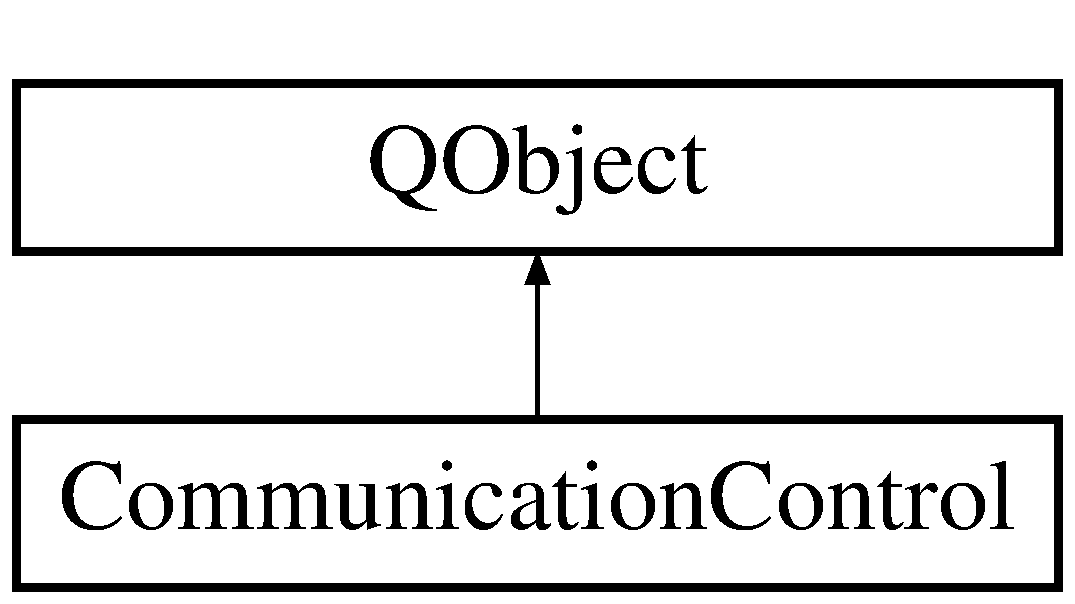
\includegraphics[height=2.000000cm]{d8/d84/a00001}
\end{center}
\end{figure}
\subsection*{Public Slots}
\subsection*{Signals}
\subsection*{Public Member Functions}
\subsection*{Static Public Member Functions}
\subsection*{Private Member Functions}
\subsection*{Private Attributes}
\subsection*{Static Private Attributes}


\subsection{Detailed Description}


\subsection{Constructor \& Destructor Documentation}
\hypertarget{a00001_a2652efe05f8aef69a18bc33ff242f6c4}{\index{Communication\-Control@{Communication\-Control}!Communication\-Control@{Communication\-Control}}
\index{Communication\-Control@{Communication\-Control}!CommunicationControl@{Communication\-Control}}
\subsubsection[{Communication\-Control}]{\setlength{\rightskip}{0pt plus 5cm}{\bf Communication\-Control} (
\begin{DoxyParamCaption}
{}
\end{DoxyParamCaption}
)\hspace{0.3cm}{\ttfamily [private]}}}\label{a00001_a2652efe05f8aef69a18bc33ff242f6c4}


Constructor. 


\begin{DoxyParams}{Parameters}
{\em none} & \\
\hline
\end{DoxyParams}

\begin{DoxyExceptions}{Exceptions}
{\em none} & \\
\hline
\end{DoxyExceptions}
\begin{DoxyReturn}{Returns}
\hyperlink{a00001}{Communication\-Control} instance 
\end{DoxyReturn}

\begin{DoxyCode}
6 \{
7     \hyperlink{a00001_acb05f93668631d777d1e9a4efa094d6e}{comThread} = \textcolor{keyword}{new} \hyperlink{a00002}{ComThread}();
8 
9     connect(\textcolor{keyword}{this}, SIGNAL(\hyperlink{a00001_a38513372e1af4752cee2e2d046c98821}{sendLaunch}()), \hyperlink{a00001_acb05f93668631d777d1e9a4efa094d6e}{comThread}, SLOT(
      \hyperlink{a00001_a38513372e1af4752cee2e2d046c98821}{sendLaunch}()));
10     connect(\textcolor{keyword}{this}, SIGNAL(\hyperlink{a00001_a2664ee66ff3ea7ed8cdca604bce4be33}{sendLand}()), \hyperlink{a00001_acb05f93668631d777d1e9a4efa094d6e}{comThread}, SLOT(\hyperlink{a00001_a2664ee66ff3ea7ed8cdca604bce4be33}{sendLand}()));
11     connect(\textcolor{keyword}{this}, SIGNAL(\hyperlink{a00001_ac898a9141e335cfee3e6c9ebb6815411}{sendHome}()), \hyperlink{a00001_acb05f93668631d777d1e9a4efa094d6e}{comThread}, SLOT(\hyperlink{a00001_ac898a9141e335cfee3e6c9ebb6815411}{sendHome}()));
12     connect(\textcolor{keyword}{this}, SIGNAL(\hyperlink{a00001_ad6b67904e4b30f5a26bef654f8a3c4a6}{sendMotOn}()), \hyperlink{a00001_acb05f93668631d777d1e9a4efa094d6e}{comThread}, SLOT(
      \hyperlink{a00001_ad6b67904e4b30f5a26bef654f8a3c4a6}{sendMotOn}()));
13     connect(\textcolor{keyword}{this}, SIGNAL(\hyperlink{a00001_a01a812308fc692593b9abcab86bf003d}{sendMotOff}()), \hyperlink{a00001_acb05f93668631d777d1e9a4efa094d6e}{comThread}, SLOT(
      \hyperlink{a00001_a01a812308fc692593b9abcab86bf003d}{sendMotOff}()));
14 
15     connect(\textcolor{keyword}{this}, SIGNAL(\hyperlink{a00001_ad6acfa8418d9902f110bee275fe13a57}{poll}(\textcolor{keywordtype}{unsigned} \textcolor{keywordtype}{short})), \hyperlink{a00001_acb05f93668631d777d1e9a4efa094d6e}{comThread}, SLOT(
      \hyperlink{a00001_ad6acfa8418d9902f110bee275fe13a57}{poll}(\textcolor{keywordtype}{unsigned} \textcolor{keywordtype}{short})));
16     connect(\hyperlink{a00001_acb05f93668631d777d1e9a4efa094d6e}{comThread}, SIGNAL(dataReceived(\textcolor{keywordtype}{char}*, \textcolor{keywordtype}{int})), \textcolor{keyword}{this}, SLOT(
      \hyperlink{a00001_ac21f894815c1cbdbf31d5bfe7d69a0af}{computePolledData}(\textcolor{keywordtype}{char}*, \textcolor{keywordtype}{int})));
17     connect(\hyperlink{a00001_acb05f93668631d777d1e9a4efa094d6e}{comThread}, SIGNAL(\hyperlink{a00001_a289c96805ddb1941fe330931d73321a0}{XBeeDisconnected}()), \textcolor{keyword}{this}, SIGNAL(
      \hyperlink{a00001_a289c96805ddb1941fe330931d73321a0}{XBeeDisconnected}()));
18     connect(\hyperlink{a00001_acb05f93668631d777d1e9a4efa094d6e}{comThread}, SIGNAL(\hyperlink{a00001_afb47495b5727dae0e7a5bac62098cb1e}{XBeeReconnected}()), \textcolor{keyword}{this}, SIGNAL(
      \hyperlink{a00001_afb47495b5727dae0e7a5bac62098cb1e}{XBeeReconnected}()));
19 
20     connect(&\hyperlink{a00001_a318ffe406e999f9b02b7e811cfc86479}{m\_pPollTimer}, SIGNAL(timeout()), \textcolor{keyword}{this}, SLOT(\hyperlink{a00001_ac02d771e0ef073ed89aeaca4ed961a05}{pollData}()));
21     connect(&\hyperlink{a00001_a0ed94524da54e5031e44ab80b249b042}{m\_pPollTimeout}, SIGNAL(timeout()), \textcolor{keyword}{this}, SLOT(
      \hyperlink{a00001_a417a5d7262b4ed5f466af6ff7878b09d}{pollDataTimedOut}()));
22     
23     connect(\hyperlink{a00001_acb05f93668631d777d1e9a4efa094d6e}{comThread}, SIGNAL(\hyperlink{a00001_a289c96805ddb1941fe330931d73321a0}{XBeeDisconnected}()), &
      \hyperlink{a00001_a3347d5764783c5008947f5addca55346}{m\_pRetryTimer}, SLOT(\hyperlink{a00001_ae262c467eec4b15d1f6e487ab6397d68}{start}()));
24     connect(&\hyperlink{a00001_a3347d5764783c5008947f5addca55346}{m\_pRetryTimer}, SIGNAL(timeout()), \textcolor{keyword}{this}, SLOT(
      \hyperlink{a00001_a7162886e6b7f34f937eefcdfdcf9a052}{retryConnection}()));
25     connect(\hyperlink{a00001_acb05f93668631d777d1e9a4efa094d6e}{comThread}, SIGNAL(\hyperlink{a00001_afb47495b5727dae0e7a5bac62098cb1e}{XBeeReconnected}()), &
      \hyperlink{a00001_a3347d5764783c5008947f5addca55346}{m\_pRetryTimer}, SLOT(\hyperlink{a00001_a8c528baf37154d347366083f0f816846}{stop}()));
26 
27     connect(\textcolor{keyword}{this}, SIGNAL(\hyperlink{a00001_afeec69b8ef45da950fab78df4a1584e3}{sendMove}(\textcolor{keywordtype}{double}, \textcolor{keywordtype}{double}, \textcolor{keywordtype}{double}, \textcolor{keywordtype}{double})), 
28         \hyperlink{a00001_acb05f93668631d777d1e9a4efa094d6e}{comThread}, SLOT(\hyperlink{a00001_afeec69b8ef45da950fab78df4a1584e3}{sendMove}(\textcolor{keywordtype}{double}, \textcolor{keywordtype}{double}, \textcolor{keywordtype}{double}, \textcolor{keywordtype}{double})));
29     connect(\textcolor{keyword}{this}, SIGNAL(\hyperlink{a00001_aabee8811f89359e4de50856e175f98e4}{sendWaypoint}(\textcolor{keywordtype}{double}, \textcolor{keywordtype}{double}, \textcolor{keywordtype}{double}, \textcolor{keywordtype}{double})),
30         \hyperlink{a00001_acb05f93668631d777d1e9a4efa094d6e}{comThread}, SLOT(\hyperlink{a00001_aabee8811f89359e4de50856e175f98e4}{sendWaypoint}(\textcolor{keywordtype}{double}, \textcolor{keywordtype}{double}, \textcolor{keywordtype}{double}, \textcolor{keywordtype}{double})));
31 
32 
33    \hyperlink{a00001_ac155e35fdeebafc89723a51520fb9fe6}{longitude} = 0;
34     \hyperlink{a00001_a76714bdbc5c536fa77dfb14533ff82a9}{latitude} = 0;
35     \hyperlink{a00001_a2b13d276aee0d9fd646c8fa3647e869b}{altitude} = 0;
36     \hyperlink{a00001_aa5a7389d7467aa0a6f4dbd964b1ce692}{m\_nLinkTries} = 0;
37 
38     \hyperlink{a00001_a7ac28e04cb63f852e31316b6fcd25228}{createLog}();
39     \hyperlink{a00001_acb05f93668631d777d1e9a4efa094d6e}{comThread}->start();
40     \hyperlink{a00001_a3347d5764783c5008947f5addca55346}{m\_pRetryTimer}.setInterval(1000);
41 \}
\end{DoxyCode}
\hypertarget{a00001_a6dd7d247ba3ce1d8ee4418f7a5a1ac68}{\index{Communication\-Control@{Communication\-Control}!$\sim$\-Communication\-Control@{$\sim$\-Communication\-Control}}
\index{$\sim$\-Communication\-Control@{$\sim$\-Communication\-Control}!CommunicationControl@{Communication\-Control}}
\subsubsection[{$\sim$\-Communication\-Control}]{\setlength{\rightskip}{0pt plus 5cm}$\sim${\bf Communication\-Control} (
\begin{DoxyParamCaption}
{}
\end{DoxyParamCaption}
)\hspace{0.3cm}{\ttfamily [private]}}}\label{a00001_a6dd7d247ba3ce1d8ee4418f7a5a1ac68}


Destructor. 


\begin{DoxyParams}{Parameters}
{\em none} & \\
\hline
\end{DoxyParams}

\begin{DoxyExceptions}{Exceptions}
{\em none} & \\
\hline
\end{DoxyExceptions}
\begin{DoxyReturn}{Returns}
none 
\end{DoxyReturn}

\begin{DoxyCode}
53 \{
54     \textcolor{keyword}{delete} \hyperlink{a00001_a7577a19e7793780c079fea7dcaefabf0}{log};
55 \}
\end{DoxyCode}


\subsection{Member Function Documentation}
\hypertarget{a00001_aaaf1f78d12176382ee56a92912b1cc53}{\index{Communication\-Control@{Communication\-Control}!autonomous\-Mode@{autonomous\-Mode}}
\index{autonomous\-Mode@{autonomous\-Mode}!CommunicationControl@{Communication\-Control}}
\subsubsection[{autonomous\-Mode}]{\setlength{\rightskip}{0pt plus 5cm}void autonomous\-Mode (
\begin{DoxyParamCaption}
{}
\end{DoxyParamCaption}
)\hspace{0.3cm}{\ttfamily [slot]}}}\label{a00001_aaaf1f78d12176382ee56a92912b1cc53}


Poll data (timed) 


\begin{DoxyParams}{Parameters}
{\em none} & \\
\hline
\end{DoxyParams}

\begin{DoxyExceptions}{Exceptions}
{\em none} & \\
\hline
\end{DoxyExceptions}
\begin{DoxyReturn}{Returns}
none 
\end{DoxyReturn}

\begin{DoxyCode}
321 \{
322     connect(\textcolor{keyword}{this}, SIGNAL(\hyperlink{a00001_aabee8811f89359e4de50856e175f98e4}{sendWaypoint}(\textcolor{keywordtype}{double}, \textcolor{keywordtype}{double}, \textcolor{keywordtype}{double}, \textcolor{keywordtype}{double})), 
323         \hyperlink{a00001_acb05f93668631d777d1e9a4efa094d6e}{comThread}, SLOT(\hyperlink{a00001_aabee8811f89359e4de50856e175f98e4}{sendWaypoint}(\textcolor{keywordtype}{double}, \textcolor{keywordtype}{double}, \textcolor{keywordtype}{double}, \textcolor{keywordtype}{double})));
324 
325     connect(\textcolor{keyword}{this}, SIGNAL(\hyperlink{a00001_a26c718e7e95e398ee9368434c23d0622}{sendGoTo}()), \hyperlink{a00001_acb05f93668631d777d1e9a4efa094d6e}{comThread}, SLOT(\hyperlink{a00001_a26c718e7e95e398ee9368434c23d0622}{sendGoTo}()));
326 \}
\end{DoxyCode}
\hypertarget{a00001_aa21c6f5ea480a2b19a771e4a232d1a4b}{\index{Communication\-Control@{Communication\-Control}!battery\-Level@{battery\-Level}}
\index{battery\-Level@{battery\-Level}!CommunicationControl@{Communication\-Control}}
\subsubsection[{battery\-Level}]{\setlength{\rightskip}{0pt plus 5cm}void battery\-Level (
\begin{DoxyParamCaption}
\item[{double}]{p\-\_\-d\-Value}
\end{DoxyParamCaption}
)\hspace{0.3cm}{\ttfamily [signal]}}}\label{a00001_aa21c6f5ea480a2b19a771e4a232d1a4b}


Battery level. 


\begin{DoxyParams}{Parameters}
{\em p\-\_\-d\-Value} & battery voltage double \\
\hline
\end{DoxyParams}

\begin{DoxyExceptions}{Exceptions}
{\em none} & \\
\hline
\end{DoxyExceptions}
\begin{DoxyReturn}{Returns}
none 
\end{DoxyReturn}
\hypertarget{a00001_ac21f894815c1cbdbf31d5bfe7d69a0af}{\index{Communication\-Control@{Communication\-Control}!compute\-Polled\-Data@{compute\-Polled\-Data}}
\index{compute\-Polled\-Data@{compute\-Polled\-Data}!CommunicationControl@{Communication\-Control}}
\subsubsection[{compute\-Polled\-Data}]{\setlength{\rightskip}{0pt plus 5cm}void compute\-Polled\-Data (
\begin{DoxyParamCaption}
\item[{char $\ast$}]{data, }
\item[{int}]{length}
\end{DoxyParamCaption}
)\hspace{0.3cm}{\ttfamily [slot]}}}\label{a00001_ac21f894815c1cbdbf31d5bfe7d69a0af}


Polled data to be sent to other modules. 


\begin{DoxyParams}{Parameters}
{\em data} & polled data char$\ast$ \\
\hline
{\em length} & length in char of the polled data int \\
\hline
\end{DoxyParams}

\begin{DoxyExceptions}{Exceptions}
{\em none} & \\
\hline
\end{DoxyExceptions}
\begin{DoxyReturn}{Returns}
none 
\end{DoxyReturn}

\begin{DoxyCode}
119 \{
120     \textcolor{keywordtype}{unsigned} \textcolor{keywordtype}{char} descriptor = 0;
121     \textcolor{keywordtype}{unsigned} \textcolor{keywordtype}{short} sendCrc = 0;
122     \textcolor{keywordtype}{unsigned} \textcolor{keywordtype}{short} checksum = 0;
123     \textcolor{keywordtype}{int} index = 0;
124     \textcolor{keywordtype}{char} ack[6];
125 
126     \hyperlink{a00001_a0ed94524da54e5031e44ab80b249b042}{m\_pPollTimeout}.stop();
127     \hyperlink{a00001_aa5a7389d7467aa0a6f4dbd964b1ce692}{m\_nLinkTries} = 0;
128     emit \hyperlink{a00001_a3a3794256db7e6b52daad0dc178c2db9}{XBeeStatus}(\textcolor{keyword}{true});
129 
130     *(\hyperlink{a00001_a7577a19e7793780c079fea7dcaefabf0}{log}->\hyperlink{a00014_abfd62a1f4f4f584858b758c0800e9b70}{getSystemLoggerStream}()) << endl << \textcolor{stringliteral}{"Compute polled data"} << endl;
131 
132     \textcolor{keywordflow}{while} (index < length)
133     \{
134         *(\hyperlink{a00001_a7577a19e7793780c079fea7dcaefabf0}{log}->\hyperlink{a00014_abfd62a1f4f4f584858b758c0800e9b70}{getSystemLoggerStream}()) << \textcolor{stringliteral}{"    End of buffer not reached : number
       of resting char = "} << length - index << endl;
135 
136         \textcolor{keywordflow}{while} (!(data[index] == \textcolor{charliteral}{'>'}))
137         \{
138             index++;
139         \}
140 
141         \textcolor{keywordflow}{if} ((data[index + 1] == \textcolor{charliteral}{'a'} && data[index + 3] == \textcolor{charliteral}{'a'} && data[index + 4] == \textcolor{charliteral}{'<'}) && index < length)
142         \{
143             \textcolor{keywordflow}{if} (index <= 395)
144             \{
145                 *(\hyperlink{a00001_a7577a19e7793780c079fea7dcaefabf0}{log}->\hyperlink{a00014_abfd62a1f4f4f584858b758c0800e9b70}{getSystemLoggerStream}()) << \textcolor{stringliteral}{"Command acknowledge received"} 
      << endl;
146                 memcpy((\textcolor{keywordtype}{void}*)ack, (\textcolor{keywordtype}{void}*)&data[index], 5 * \textcolor{keyword}{sizeof}(\textcolor{keywordtype}{char}));
147                 ack[5] = \textcolor{charliteral}{'\(\backslash\)0'};
148             \}
149 
150             emit \hyperlink{a00001_a49a7c28f7c937cffeef6878cec48b396}{displayAck}(ack);
151         \}
152         \textcolor{keywordflow}{else} \textcolor{keywordflow}{if} ((data[index + 1] == \textcolor{charliteral}{'*'} && data[index + 2] == \textcolor{charliteral}{'>'}) && index < length - \textcolor{keyword}{sizeof}(\textcolor{stringliteral}{">*>"}) - 1 -
       \textcolor{keyword}{sizeof}(\textcolor{keywordtype}{short}))
153         \{
154             *(\hyperlink{a00001_a7577a19e7793780c079fea7dcaefabf0}{log}->\hyperlink{a00014_abfd62a1f4f4f584858b758c0800e9b70}{getSystemLoggerStream}()) << \textcolor{stringliteral}{"    New polled data structure found
       at index "} << index << endl;
155 
156             descriptor = data[index + \textcolor{keyword}{sizeof}(\textcolor{stringliteral}{">*>"}) - 1 + \textcolor{keyword}{sizeof}(\textcolor{keywordtype}{short})];
157             index += \textcolor{keyword}{sizeof}(\textcolor{stringliteral}{">*>"}) - 1 + \textcolor{keyword}{sizeof}(\textcolor{keywordtype}{short}) + \textcolor{keyword}{sizeof}(char);
158 
159             \textcolor{keywordflow}{if} (descriptor == STATUS\_DESCRIPTOR)
160             \{
161                 *(\hyperlink{a00001_a7577a19e7793780c079fea7dcaefabf0}{log}->\hyperlink{a00014_abfd62a1f4f4f584858b758c0800e9b70}{getSystemLoggerStream}()) << \textcolor{stringliteral}{"        Status polled data
       found in buffer"} << endl;
162 
163                 \textcolor{keywordflow}{if} (index < (length - \textcolor{keyword}{sizeof}(\hyperlink{a00004_df/d98/a00107}{LL\_STATUS}) - \textcolor{keyword}{sizeof}(\textcolor{keywordtype}{short}) + \textcolor{keyword}{sizeof}(\textcolor{stringliteral}{"<#<"}) - 1))
164                 \{
165                     memcpy((\textcolor{keywordtype}{void}*)&\hyperlink{a00001_aab0e6d0ec390cd7a3094356a2bc5354e}{st}, &data[index], \textcolor{keyword}{sizeof}(\hyperlink{a00004_df/d98/a00107}{LL\_STATUS}));
166 
167                     index += \textcolor{keyword}{sizeof}(\hyperlink{a00004_df/d98/a00107}{LL\_STATUS});
168                     memcpy((\textcolor{keywordtype}{void}*)&sendCrc, &data[index], \textcolor{keyword}{sizeof}(\textcolor{keywordtype}{short}));
169 
170                     checksum = \hyperlink{a00001_a914607c9e5f387852e494b819d9da3dd}{crc16}(&\hyperlink{a00001_aab0e6d0ec390cd7a3094356a2bc5354e}{st}, \textcolor{keyword}{sizeof}(\hyperlink{a00004_df/d98/a00107}{LL\_STATUS}));
171 
172                     emit \hyperlink{a00001_aa21c6f5ea480a2b19a771e4a232d1a4b}{batteryLevel}(\hyperlink{a00001_aab0e6d0ec390cd7a3094356a2bc5354e}{st}.\hyperlink{a00004_a459f77aee98b6bebbd3c2d54f2ab6667}{battery\_voltage\_1} / 1000.);
173                     emit \hyperlink{a00001_ac07c6c4960d3789765cee7bc68a5fe44}{updateStatus}(\hyperlink{a00001_aab0e6d0ec390cd7a3094356a2bc5354e}{st}.\hyperlink{a00004_a3a9b579ed098eba7a5107adb32a9375a}{flightMode});
174                     
175                     emit \hyperlink{a00001_a5f730a9a91784cbf28d39ab22e4d7fec}{inFlight}(\hyperlink{a00001_aab0e6d0ec390cd7a3094356a2bc5354e}{st}.\hyperlink{a00004_af2fb6251c4d6d896f8b035e3b0f20f62}{flying});
176                 \}
177                 \textcolor{keywordflow}{else}
178                 \{
179                     *(\hyperlink{a00001_a7577a19e7793780c079fea7dcaefabf0}{log}->\hyperlink{a00014_abfd62a1f4f4f584858b758c0800e9b70}{getSystemLoggerStream}()) << \textcolor{stringliteral}{"        ERROR : Incomplete
       structure"} << endl;
180                 \}
181             \}
182             \textcolor{keywordflow}{else} \textcolor{keywordflow}{if} (descriptor == IMU\_CALCDATA\_DESCRIPTOR)
183             \{
184                 *(\hyperlink{a00001_a7577a19e7793780c079fea7dcaefabf0}{log}->\hyperlink{a00014_abfd62a1f4f4f584858b758c0800e9b70}{getSystemLoggerStream}()) << \textcolor{stringliteral}{"        IMU polled data found
       in buffer"} << endl;
185 
186                 \textcolor{keywordflow}{if} (index < (length - \textcolor{keyword}{sizeof}(\hyperlink{a00004_d7/d70/a00106}{IMU\_CALCDATA}) - \textcolor{keyword}{sizeof}(\textcolor{keywordtype}{short}) + \textcolor{keyword}{sizeof}(\textcolor{stringliteral}{"<#<"}) - 1)
      )
187                 \{
188                     memcpy((\textcolor{keywordtype}{void}*)&\hyperlink{a00001_a8e97a0fe2d5d03eb1a9344f36f8b6b85}{imu}, &data[index], \textcolor{keyword}{sizeof}(\hyperlink{a00004_d7/d70/a00106}{IMU\_CALCDATA}));
189 
190                     index += \textcolor{keyword}{sizeof}(\hyperlink{a00004_d7/d70/a00106}{IMU\_CALCDATA});
191                     memcpy((\textcolor{keywordtype}{void}*)&sendCrc, &data[index], \textcolor{keyword}{sizeof}(\textcolor{keywordtype}{short}));
192 
193                     checksum = \hyperlink{a00001_a914607c9e5f387852e494b819d9da3dd}{crc16}(&\hyperlink{a00001_a8e97a0fe2d5d03eb1a9344f36f8b6b85}{imu}, \textcolor{keyword}{sizeof}(\hyperlink{a00004_d7/d70/a00106}{IMU\_CALCDATA}));
194                     \hyperlink{a00001_ae024163074f229a06b7ea69b190e466d}{heading} = \hyperlink{a00001_a8e97a0fe2d5d03eb1a9344f36f8b6b85}{imu}.\hyperlink{a00004_ac66ed08857aecb91f07bdc414b445973}{mag\_heading} / 1000.;
195                     \hyperlink{a00001_a89f6abd564014faeff7cd20c340a9c7d}{height} = \hyperlink{a00001_a8e97a0fe2d5d03eb1a9344f36f8b6b85}{imu}.\hyperlink{a00004_ad12fc34ce789bce6c8a05d8a17138534}{height} / 1000.;
196 
197                     emit \hyperlink{a00001_aa3c54f0958638486df2b69a9b53c5d7f}{updateHeading}(\hyperlink{a00001_ae024163074f229a06b7ea69b190e466d}{heading});
198                     emit \hyperlink{a00001_a5114b66563f0437e0f1eac070557cb4c}{updateHeight}(\hyperlink{a00001_a89f6abd564014faeff7cd20c340a9c7d}{height});
199                 \}
200                 \textcolor{keywordflow}{else}
201                 \{
202                     *(\hyperlink{a00001_a7577a19e7793780c079fea7dcaefabf0}{log}->\hyperlink{a00014_abfd62a1f4f4f584858b758c0800e9b70}{getSystemLoggerStream}()) << \textcolor{stringliteral}{"        ERROR : Incomplete
       structure"} << endl;
203                 \}
204             \}
205             \textcolor{keywordflow}{else} \textcolor{keywordflow}{if} (descriptor == CURRENT\_WAY\_DESCRIPTOR)
206             \{
207                 *(\hyperlink{a00001_a7577a19e7793780c079fea7dcaefabf0}{log}->\hyperlink{a00014_abfd62a1f4f4f584858b758c0800e9b70}{getSystemLoggerStream}()) << \textcolor{stringliteral}{"        Current way polled data
       found in buffer"} << endl;
208 
209                 \textcolor{keywordflow}{if} (index < (length - \textcolor{keyword}{sizeof}(\hyperlink{a00004_d1/d84/a00052}{CURRENT\_WAY}) - \textcolor{keyword}{sizeof}(\textcolor{keywordtype}{short}) + \textcolor{keyword}{sizeof}(\textcolor{stringliteral}{"<#<"}) - 1))
210                 \{
211                     memcpy((\textcolor{keywordtype}{void}*)&\hyperlink{a00001_a4c9b6ed9e971686ce98aa7170cb1e7f2}{cw}, &data[index], \textcolor{keyword}{sizeof}(\hyperlink{a00004_d1/d84/a00052}{CURRENT\_WAY}));
212 
213                     index += \textcolor{keyword}{sizeof}(\hyperlink{a00004_d1/d84/a00052}{CURRENT\_WAY});
214                     memcpy((\textcolor{keywordtype}{void}*)&sendCrc, &data[index], \textcolor{keyword}{sizeof}(\textcolor{keywordtype}{short}));
215 
216                     checksum = \hyperlink{a00001_a914607c9e5f387852e494b819d9da3dd}{crc16}(&\hyperlink{a00001_a4c9b6ed9e971686ce98aa7170cb1e7f2}{cw}, \textcolor{keyword}{sizeof}(\hyperlink{a00004_d1/d84/a00052}{CURRENT\_WAY}));
217 
218                     emit \hyperlink{a00001_a6f8056c0ce5dd09565148cff2aa1d6aa}{waypointNAVInfo}(\hyperlink{a00001_a4c9b6ed9e971686ce98aa7170cb1e7f2}{cw}.\hyperlink{a00004_a62b91a02c0e7c93551d2875c725ad883}{current\_wp}, 
      \hyperlink{a00001_a4c9b6ed9e971686ce98aa7170cb1e7f2}{cw}.\hyperlink{a00004_adba24dc812335f36e8793c535dc6e8bf}{distance\_to\_wp} / 10., \hyperlink{a00001_a4c9b6ed9e971686ce98aa7170cb1e7f2}{cw}.\hyperlink{a00004_a820db34ea9303c6b8f6266107b434058}{navigation\_status});
219                 \}
220                 \textcolor{keywordflow}{else}
221                 \{
222                     *(\hyperlink{a00001_a7577a19e7793780c079fea7dcaefabf0}{log}->\hyperlink{a00014_abfd62a1f4f4f584858b758c0800e9b70}{getSystemLoggerStream}()) << \textcolor{stringliteral}{"        ERROR : Incomplete
       structure"} << endl;
223                 \}
224             \}
225             \textcolor{keywordflow}{else} \textcolor{keywordflow}{if} (descriptor == GPS\_DESCRIPTOR && index < (length - \textcolor{keyword}{sizeof}(
      \hyperlink{a00004_d3/d32/a00105}{GPS\_DATA\_ADVANCED}) - \textcolor{keyword}{sizeof}(\textcolor{keywordtype}{short}) + \textcolor{keyword}{sizeof}(\textcolor{stringliteral}{"<#<"}) - 1))
226             \{
227                 *(\hyperlink{a00001_a7577a19e7793780c079fea7dcaefabf0}{log}->\hyperlink{a00014_abfd62a1f4f4f584858b758c0800e9b70}{getSystemLoggerStream}()) << \textcolor{stringliteral}{"        Geolocation polled data
       found in buffer"} << endl;
228 
229                 \textcolor{keywordflow}{if} (index < (length - \textcolor{keyword}{sizeof}(\hyperlink{a00004_d3/d32/a00105}{GPS\_DATA\_ADVANCED}) - \textcolor{keyword}{sizeof}(\textcolor{keywordtype}{short}) + \textcolor{keyword}{sizeof}(\textcolor{stringliteral}{"
      <#<"}) - 1))
230                 \{
231                     memcpy((\textcolor{keywordtype}{void}*)&\hyperlink{a00001_ac042d2d437c63ce6fe1916aac1c77a9b}{gps}, &data[index], \textcolor{keyword}{sizeof}(
      \hyperlink{a00004_d3/d32/a00105}{GPS\_DATA\_ADVANCED}));
232 
233                     index += \textcolor{keyword}{sizeof}(\hyperlink{a00004_d3/d32/a00105}{GPS\_DATA\_ADVANCED});
234                     memcpy((\textcolor{keywordtype}{void}*)&sendCrc, &data[index], \textcolor{keyword}{sizeof}(\textcolor{keywordtype}{short}));
235 
236                     checksum = \hyperlink{a00001_a914607c9e5f387852e494b819d9da3dd}{crc16}(&\hyperlink{a00001_ac042d2d437c63ce6fe1916aac1c77a9b}{gps}, \textcolor{keyword}{sizeof}(\hyperlink{a00004_d3/d32/a00105}{GPS\_DATA\_ADVANCED}));
237 
238                     \hyperlink{a00001_ac155e35fdeebafc89723a51520fb9fe6}{longitude} = \hyperlink{a00001_ac042d2d437c63ce6fe1916aac1c77a9b}{gps}.\hyperlink{a00004_a17963aafb9acb082fcc06c90195cb4fa}{longitude} / 10000000.;
239                     \hyperlink{a00001_a76714bdbc5c536fa77dfb14533ff82a9}{latitude} = \hyperlink{a00001_ac042d2d437c63ce6fe1916aac1c77a9b}{gps}.\hyperlink{a00004_a5bf9aac20fe4e7a73cd1a9fc30d7ae00}{latitude} / 10000000.;
240                     \hyperlink{a00001_a2b13d276aee0d9fd646c8fa3647e869b}{altitude} = \hyperlink{a00001_ac042d2d437c63ce6fe1916aac1c77a9b}{gps}.\hyperlink{a00004_ad12fc34ce789bce6c8a05d8a17138534}{height} / 1000.;
241                     \textcolor{keywordtype}{double} speedX = qAbs(\hyperlink{a00001_ac042d2d437c63ce6fe1916aac1c77a9b}{gps}.\hyperlink{a00004_a20fcaf3d7d5effa75ca571510f53a6cc}{speed\_x} * 0.0036);
242                     \textcolor{keywordtype}{double} speedY = qAbs(\hyperlink{a00001_ac042d2d437c63ce6fe1916aac1c77a9b}{gps}.\hyperlink{a00004_a3abd5cb27c81871612651aee8a0476ba}{speed\_y} * 0.0036);
243                     \hyperlink{a00001_a9747f19755c0d74510f7a0860c11fbef}{m\_dSpeed} = qSqrt(speedX * speedX + speedY * speedY);
244 
245                     \textcolor{keywordflow}{if} (checksum == sendCrc)
246                     \{
247                         emit \hyperlink{a00001_ac64f2ec114d4ab8dd8ed8dd31f243454}{geolocation}(\hyperlink{a00001_a76714bdbc5c536fa77dfb14533ff82a9}{latitude}, \hyperlink{a00001_ac155e35fdeebafc89723a51520fb9fe6}{longitude}, 
      \hyperlink{a00001_a2b13d276aee0d9fd646c8fa3647e869b}{altitude}, \hyperlink{a00001_ae024163074f229a06b7ea69b190e466d}{heading});
248                         emit \hyperlink{a00001_aeffc2ecc4a5de587172d46c5ff0156db}{updateSpeed}(\hyperlink{a00001_a9747f19755c0d74510f7a0860c11fbef}{m\_dSpeed});
249                         emit \hyperlink{a00001_a8ca9715733ba2afa7525da56a6e98311}{updateGPSQuality}(\hyperlink{a00001_ac042d2d437c63ce6fe1916aac1c77a9b}{gps}.\hyperlink{a00004_a9390419b61f0e0bae53f5f094ce82b93}{numSV});
250                     \}
251                 \}
252                 \textcolor{keywordflow}{else}
253                 \{
254                     *(\hyperlink{a00001_a7577a19e7793780c079fea7dcaefabf0}{log}->\hyperlink{a00014_abfd62a1f4f4f584858b758c0800e9b70}{getSystemLoggerStream}()) << \textcolor{stringliteral}{"        ERROR : Incomplete
       structure"} << endl;
255                 \}
256 
257                 \hyperlink{a00001_a31082f0cdd2aeea81ceb79028bf639af}{writeLog}(checksum == sendCrc);
258             \}
259             \textcolor{keywordflow}{else} \textcolor{keywordflow}{if} (descriptor == RC\_DATA\_DESCRIPTOR && index < (length - \textcolor{keyword}{sizeof}(
      \hyperlink{a00004_d1/dd6/a00108}{RC\_DATA}) - \textcolor{keyword}{sizeof}(\textcolor{keywordtype}{short}) + \textcolor{keyword}{sizeof}(\textcolor{stringliteral}{"<#<"}) - 1))
260             \{
261                 *(\hyperlink{a00001_a7577a19e7793780c079fea7dcaefabf0}{log}->\hyperlink{a00014_abfd62a1f4f4f584858b758c0800e9b70}{getSystemLoggerStream}()) << \textcolor{stringliteral}{"        RC polled data found in
       buffer"} << endl;
262 
263                 \textcolor{keywordflow}{if} (index < (length - \textcolor{keyword}{sizeof}(\hyperlink{a00004_d1/dd6/a00108}{RC\_DATA}) - \textcolor{keyword}{sizeof}(\textcolor{keywordtype}{short}) + \textcolor{keyword}{sizeof}(\textcolor{stringliteral}{"<#<"}) - 1))
264                 \{
265                     memcpy((\textcolor{keywordtype}{void}*)&\hyperlink{a00001_a53109ee6a15f404839038d5405afaee1}{rc}, &data[index], \textcolor{keyword}{sizeof}(\hyperlink{a00004_d1/dd6/a00108}{RC\_DATA}));
266 
267                     index += \textcolor{keyword}{sizeof}(\hyperlink{a00004_d1/dd6/a00108}{RC\_DATA});
268                     memcpy((\textcolor{keywordtype}{void}*)&sendCrc, &data[index], \textcolor{keyword}{sizeof}(\textcolor{keywordtype}{short}));
269 
270                     checksum = \hyperlink{a00001_a914607c9e5f387852e494b819d9da3dd}{crc16}(&\hyperlink{a00001_a53109ee6a15f404839038d5405afaee1}{rc}, \textcolor{keyword}{sizeof}(\hyperlink{a00004_d1/dd6/a00108}{RC\_DATA}));
271 
272                     emit \hyperlink{a00001_ab51c3c4f71404589fc3a47c213449b1e}{rcData}(\hyperlink{a00001_a53109ee6a15f404839038d5405afaee1}{rc}.\hyperlink{a00004_a9ece938051bc16291613a2bdccd52bec}{channels\_out}[3], \hyperlink{a00001_a53109ee6a15f404839038d5405afaee1}{rc}.
      \hyperlink{a00004_a9ece938051bc16291613a2bdccd52bec}{channels\_out}[0], \hyperlink{a00001_a53109ee6a15f404839038d5405afaee1}{rc}.\hyperlink{a00004_a9ece938051bc16291613a2bdccd52bec}{channels\_out}[1], 
273                             \hyperlink{a00001_a53109ee6a15f404839038d5405afaee1}{rc}.\hyperlink{a00004_a9ece938051bc16291613a2bdccd52bec}{channels\_out}[2], \hyperlink{a00001_a53109ee6a15f404839038d5405afaee1}{rc}.\hyperlink{a00004_a9ece938051bc16291613a2bdccd52bec}{channels\_out}[4], 
      \hyperlink{a00001_a53109ee6a15f404839038d5405afaee1}{rc}.\hyperlink{a00004_a9ece938051bc16291613a2bdccd52bec}{channels\_out}[5], \hyperlink{a00001_a53109ee6a15f404839038d5405afaee1}{rc}.\hyperlink{a00004_a6ae861576031be7ecfd4d6c9e870fb99}{lock});
274                 \}
275                 \textcolor{keywordflow}{else}
276                 \{
277                     *(\hyperlink{a00001_a7577a19e7793780c079fea7dcaefabf0}{log}->\hyperlink{a00014_abfd62a1f4f4f584858b758c0800e9b70}{getSystemLoggerStream}()) << \textcolor{stringliteral}{"        ERROR : Incomplete
       structure"} << endl;
278                 \}
279             \}
280             \textcolor{keywordflow}{else}
281             \{
282                 *(\hyperlink{a00001_a7577a19e7793780c079fea7dcaefabf0}{log}->\hyperlink{a00014_abfd62a1f4f4f584858b758c0800e9b70}{getSystemLoggerStream}()) << \textcolor{stringliteral}{"        Unknown polled data
       type found in buffer"} << endl;
283             \}
284         \}
285         index += \textcolor{keyword}{sizeof}(short) + \textcolor{keyword}{sizeof}(\textcolor{stringliteral}{"<#<"}) - 1;
286     \}
287 
288     *(\hyperlink{a00001_a7577a19e7793780c079fea7dcaefabf0}{log}->\hyperlink{a00014_abfd62a1f4f4f584858b758c0800e9b70}{getSystemLoggerStream}()) << \textcolor{stringliteral}{"Polled data sent"} << endl;
289 \}
\end{DoxyCode}
\hypertarget{a00001_a57866bb7255c471cd9c4cfdf7c88681d}{\index{Communication\-Control@{Communication\-Control}!computer\-Aided\-Control\-Mode@{computer\-Aided\-Control\-Mode}}
\index{computer\-Aided\-Control\-Mode@{computer\-Aided\-Control\-Mode}!CommunicationControl@{Communication\-Control}}
\subsubsection[{computer\-Aided\-Control\-Mode}]{\setlength{\rightskip}{0pt plus 5cm}void computer\-Aided\-Control\-Mode (
\begin{DoxyParamCaption}
{}
\end{DoxyParamCaption}
)\hspace{0.3cm}{\ttfamily [slot]}}}\label{a00001_a57866bb7255c471cd9c4cfdf7c88681d}


Poll data (timed) 


\begin{DoxyParams}{Parameters}
{\em none} & \\
\hline
\end{DoxyParams}

\begin{DoxyExceptions}{Exceptions}
{\em none} & \\
\hline
\end{DoxyExceptions}
\begin{DoxyReturn}{Returns}
none 
\end{DoxyReturn}

\begin{DoxyCode}
329 \{
330     disconnect(\textcolor{keyword}{this}, SIGNAL(\hyperlink{a00001_aabee8811f89359e4de50856e175f98e4}{sendWaypoint}(\textcolor{keywordtype}{double}, \textcolor{keywordtype}{double}, \textcolor{keywordtype}{double}, \textcolor{keywordtype}{double})), 
331         \hyperlink{a00001_acb05f93668631d777d1e9a4efa094d6e}{comThread}, SLOT(\hyperlink{a00001_aabee8811f89359e4de50856e175f98e4}{sendWaypoint}(\textcolor{keywordtype}{double}, \textcolor{keywordtype}{double}, \textcolor{keywordtype}{double}, \textcolor{keywordtype}{double})));
332 
333     disconnect(\textcolor{keyword}{this}, SIGNAL(\hyperlink{a00001_a26c718e7e95e398ee9368434c23d0622}{sendGoTo}()), \hyperlink{a00001_acb05f93668631d777d1e9a4efa094d6e}{comThread}, SLOT(
      \hyperlink{a00001_a26c718e7e95e398ee9368434c23d0622}{sendGoTo}()));
334 \}
\end{DoxyCode}
\hypertarget{a00001_a4c881076a61ae41ab4b5e0a615b442b6}{\index{Communication\-Control@{Communication\-Control}!control\-Waypoint@{control\-Waypoint}}
\index{control\-Waypoint@{control\-Waypoint}!CommunicationControl@{Communication\-Control}}
\subsubsection[{control\-Waypoint}]{\setlength{\rightskip}{0pt plus 5cm}void control\-Waypoint (
\begin{DoxyParamCaption}
\item[{double}]{x\-Dest, }
\item[{double}]{y\-Dest, }
\item[{double}]{z\-Dest}
\end{DoxyParamCaption}
)\hspace{0.3cm}{\ttfamily [slot]}}}\label{a00001_a4c881076a61ae41ab4b5e0a615b442b6}


Control the given waypoint validity. 


\begin{DoxyParams}{Parameters}
{\em x\-Dest} & longitude double \\
\hline
{\em y\-Dest} & latitude double \\
\hline
{\em z\-Dest} & altitude double \\
\hline
\end{DoxyParams}

\begin{DoxyExceptions}{Exceptions}
{\em none} & \\
\hline
\end{DoxyExceptions}
\begin{DoxyReturn}{Returns}
none 
\end{DoxyReturn}

\begin{DoxyCode}
81 \{
82     \textcolor{keywordtype}{int} raver = 6378137;
83 
84     qreal xRad = xDest * M\_PI / 180.;
85     qreal yRad = yDest * M\_PI / 180.;
86     qreal latRad = \hyperlink{a00001_a76714bdbc5c536fa77dfb14533ff82a9}{latitude} * M\_PI / 180.;
87     qreal longRad = \hyperlink{a00001_ac155e35fdeebafc89723a51520fb9fe6}{longitude} * M\_PI / 180.;
88 
89     qreal dist = raver * qAcos((qCos(yRad) * qCos(latRad) * qCos(xRad - longRad)) + (qSin(yRad) * qSin(
      latRad)));
90 
91     \textcolor{keywordtype}{bool} validDistance = dist <= DISTMAX;
92     \textcolor{keywordtype}{bool} validAltitude = (zDest > \hyperlink{a00001_a2b13d276aee0d9fd646c8fa3647e869b}{altitude}) && (zDest <= \hyperlink{a00001_a2b13d276aee0d9fd646c8fa3647e869b}{altitude} + ALTMAX);
93 
94     emit \hyperlink{a00001_acc446efda119ee2dd0b845a4e96b3397}{validWaypoint}(dist, validDistance, validAltitude);
95 \}
\end{DoxyCode}
\hypertarget{a00001_a914607c9e5f387852e494b819d9da3dd}{\index{Communication\-Control@{Communication\-Control}!crc16@{crc16}}
\index{crc16@{crc16}!CommunicationControl@{Communication\-Control}}
\subsubsection[{crc16}]{\setlength{\rightskip}{0pt plus 5cm}unsigned short crc16 (
\begin{DoxyParamCaption}
\item[{void $\ast$}]{data, }
\item[{unsigned short}]{cnt}
\end{DoxyParamCaption}
)}}\label{a00001_a914607c9e5f387852e494b819d9da3dd}


Compute crc. 


\begin{DoxyParams}{Parameters}
{\em none} & \\
\hline
\end{DoxyParams}

\begin{DoxyExceptions}{Exceptions}
{\em none} & \\
\hline
\end{DoxyExceptions}
\begin{DoxyReturn}{Returns}
none 
\end{DoxyReturn}

\begin{DoxyCode}
105 \{
106     \textcolor{keywordtype}{unsigned} \textcolor{keywordtype}{short} crc = 0xff;
107     \textcolor{keywordtype}{unsigned} \textcolor{keywordtype}{char} *ptr = (\textcolor{keywordtype}{unsigned} \textcolor{keywordtype}{char} *)data;
108     \textcolor{keywordtype}{int} i;
109 
110     \textcolor{keywordflow}{for} (i = 0; i < cnt; i++)
111     \{
112         crc = \hyperlink{a00001_af69ddfcaef7d003a3ac128b9f33ca1ba}{crc\_update}(crc, *ptr);
113         ptr++;
114     \}
115     \textcolor{keywordflow}{return} crc;
116 \}
\end{DoxyCode}
\hypertarget{a00001_af69ddfcaef7d003a3ac128b9f33ca1ba}{\index{Communication\-Control@{Communication\-Control}!crc\-\_\-update@{crc\-\_\-update}}
\index{crc\-\_\-update@{crc\-\_\-update}!CommunicationControl@{Communication\-Control}}
\subsubsection[{crc\-\_\-update}]{\setlength{\rightskip}{0pt plus 5cm}unsigned short crc\-\_\-update (
\begin{DoxyParamCaption}
\item[{unsigned short}]{crc, }
\item[{unsigned char}]{data}
\end{DoxyParamCaption}
)}}\label{a00001_af69ddfcaef7d003a3ac128b9f33ca1ba}


Update crc. 


\begin{DoxyParams}{Parameters}
{\em none} & \\
\hline
\end{DoxyParams}

\begin{DoxyExceptions}{Exceptions}
{\em none} & \\
\hline
\end{DoxyExceptions}
\begin{DoxyReturn}{Returns}
none 
\end{DoxyReturn}

\begin{DoxyCode}
98 \{
99     data ^= (crc & 0xff);
100     data ^= data << 4;
101     \textcolor{keywordflow}{return} ((((\textcolor{keywordtype}{unsigned} \textcolor{keywordtype}{short}) data << 8) | ((crc >> 8) & 0xff)) ^ (\textcolor{keywordtype}{unsigned} char) (data >> 4) ^ ((\textcolor{keywordtype}{unsigned}
       short) data << 3));
102 \}
\end{DoxyCode}
\hypertarget{a00001_a7ac28e04cb63f852e31316b6fcd25228}{\index{Communication\-Control@{Communication\-Control}!create\-Log@{create\-Log}}
\index{create\-Log@{create\-Log}!CommunicationControl@{Communication\-Control}}
\subsubsection[{create\-Log}]{\setlength{\rightskip}{0pt plus 5cm}void create\-Log (
\begin{DoxyParamCaption}
{}
\end{DoxyParamCaption}
)}}\label{a00001_a7ac28e04cb63f852e31316b6fcd25228}


Create logger. 


\begin{DoxyParams}{Parameters}
{\em none} & \\
\hline
\end{DoxyParams}

\begin{DoxyExceptions}{Exceptions}
{\em none} & \\
\hline
\end{DoxyExceptions}
\begin{DoxyReturn}{Returns}
none 
\end{DoxyReturn}

\begin{DoxyCode}
292 \{
293     \hyperlink{a00001_a7577a19e7793780c079fea7dcaefabf0}{log} = \textcolor{keyword}{new} \hyperlink{a00014}{UAVLogger}();
294 
295     *(\hyperlink{a00001_a7577a19e7793780c079fea7dcaefabf0}{log}->\hyperlink{a00014_aeabc1d456526485e8c922a94b4bfa22d}{getDataLoggerStream}()) << \textcolor{stringliteral}{"Date"} << \textcolor{stringliteral}{"; "} << \textcolor{stringliteral}{"Latitude (�)"} << \textcolor{stringliteral}{"; "} << \textcolor{stringliteral}{"
      Longitude (�)"} 
296         << \textcolor{stringliteral}{"; "} << \textcolor{stringliteral}{"Altitude (from ground, in m)"} << \textcolor{stringliteral}{"; "} << \textcolor{stringliteral}{"Heading (�)"} << \textcolor{stringliteral}{"; "} 
297         << \textcolor{stringliteral}{"Speed (km/h)"} << \textcolor{stringliteral}{"; "} << \textcolor{stringliteral}{"Valid crc"} << endl;
298 \}
\end{DoxyCode}
\hypertarget{a00001_a49a7c28f7c937cffeef6878cec48b396}{\index{Communication\-Control@{Communication\-Control}!display\-Ack@{display\-Ack}}
\index{display\-Ack@{display\-Ack}!CommunicationControl@{Communication\-Control}}
\subsubsection[{display\-Ack}]{\setlength{\rightskip}{0pt plus 5cm}void display\-Ack (
\begin{DoxyParamCaption}
\item[{char $\ast$}]{data}
\end{DoxyParamCaption}
)\hspace{0.3cm}{\ttfamily [signal]}}}\label{a00001_a49a7c28f7c937cffeef6878cec48b396}


Update acknowledge value. 


\begin{DoxyParams}{Parameters}
{\em data} & received acknowledge char$\ast$ \\
\hline
\end{DoxyParams}

\begin{DoxyExceptions}{Exceptions}
{\em none} & \\
\hline
\end{DoxyExceptions}
\begin{DoxyReturn}{Returns}
none 
\end{DoxyReturn}
\hypertarget{a00001_ac64f2ec114d4ab8dd8ed8dd31f243454}{\index{Communication\-Control@{Communication\-Control}!geolocation@{geolocation}}
\index{geolocation@{geolocation}!CommunicationControl@{Communication\-Control}}
\subsubsection[{geolocation}]{\setlength{\rightskip}{0pt plus 5cm}void geolocation (
\begin{DoxyParamCaption}
\item[{double}]{latitude, }
\item[{double}]{longitude, }
\item[{double}]{altitude, }
\item[{double}]{heading}
\end{DoxyParamCaption}
)\hspace{0.3cm}{\ttfamily [signal]}}}\label{a00001_ac64f2ec114d4ab8dd8ed8dd31f243454}


Update M\-U\-A\-V geolocation. 


\begin{DoxyParams}{Parameters}
{\em x} & longitude double \\
\hline
{\em y} & latitude double \\
\hline
{\em z} & altitude double \\
\hline
{\em yaw} & heading double \\
\hline
\end{DoxyParams}

\begin{DoxyExceptions}{Exceptions}
{\em none} & \\
\hline
\end{DoxyExceptions}
\begin{DoxyReturn}{Returns}
none 
\end{DoxyReturn}
\hypertarget{a00001_afebd43c1f2afd7ec0eb35f99e50f0964}{\index{Communication\-Control@{Communication\-Control}!get\-Instance@{get\-Instance}}
\index{get\-Instance@{get\-Instance}!CommunicationControl@{Communication\-Control}}
\subsubsection[{get\-Instance}]{\setlength{\rightskip}{0pt plus 5cm}{\bf Communication\-Control} $\ast$ get\-Instance (
\begin{DoxyParamCaption}
{}
\end{DoxyParamCaption}
)\hspace{0.3cm}{\ttfamily [static]}}}\label{a00001_afebd43c1f2afd7ec0eb35f99e50f0964}


Lone instance getter. 


\begin{DoxyParams}{Parameters}
{\em none} & \\
\hline
\end{DoxyParams}

\begin{DoxyExceptions}{Exceptions}
{\em none} & \\
\hline
\end{DoxyExceptions}
\begin{DoxyReturn}{Returns}
lone instance Communication\-Control$\ast$ 
\end{DoxyReturn}

\begin{DoxyCode}
71 \{
72     \textcolor{keywordflow}{if} (\hyperlink{a00001_aee0300254b12ae17cc030042d51787c4}{singleton} == NULL)
73     \{
74         \hyperlink{a00001_aee0300254b12ae17cc030042d51787c4}{singleton} = \textcolor{keyword}{new} \hyperlink{a00001_a2652efe05f8aef69a18bc33ff242f6c4}{CommunicationControl}();
75     \}
76 
77     \textcolor{keywordflow}{return} \hyperlink{a00001_aee0300254b12ae17cc030042d51787c4}{singleton};
78 \}
\end{DoxyCode}
\hypertarget{a00001_ade64afbb6a24f22d48cff310655c8755}{\index{Communication\-Control@{Communication\-Control}!get\-Logger@{get\-Logger}}
\index{get\-Logger@{get\-Logger}!CommunicationControl@{Communication\-Control}}
\subsubsection[{get\-Logger}]{\setlength{\rightskip}{0pt plus 5cm}{\bf U\-A\-V\-Logger} $\ast$ get\-Logger (
\begin{DoxyParamCaption}
{}
\end{DoxyParamCaption}
)}}\label{a00001_ade64afbb6a24f22d48cff310655c8755}


Logger getter. 


\begin{DoxyParams}{Parameters}
{\em none} & \\
\hline
\end{DoxyParams}

\begin{DoxyExceptions}{Exceptions}
{\em none} & \\
\hline
\end{DoxyExceptions}
\begin{DoxyReturn}{Returns}
logger U\-A\-V\-Logger$\ast$ 
\end{DoxyReturn}

\begin{DoxyCode}
309 \{
310     \textcolor{keywordflow}{return} \hyperlink{a00001_a7577a19e7793780c079fea7dcaefabf0}{log};
311 \}
\end{DoxyCode}
\hypertarget{a00001_a5f730a9a91784cbf28d39ab22e4d7fec}{\index{Communication\-Control@{Communication\-Control}!in\-Flight@{in\-Flight}}
\index{in\-Flight@{in\-Flight}!CommunicationControl@{Communication\-Control}}
\subsubsection[{in\-Flight}]{\setlength{\rightskip}{0pt plus 5cm}void in\-Flight (
\begin{DoxyParamCaption}
\item[{char}]{p\-\_\-c\-Value}
\end{DoxyParamCaption}
)\hspace{0.3cm}{\ttfamily [signal]}}}\label{a00001_a5f730a9a91784cbf28d39ab22e4d7fec}


Update flight state. 


\begin{DoxyParams}{Parameters}
{\em p\-\_\-c\-Value} & flight in progress (engines started) char \\
\hline
\end{DoxyParams}

\begin{DoxyExceptions}{Exceptions}
{\em none} & \\
\hline
\end{DoxyExceptions}
\begin{DoxyReturn}{Returns}
none 
\end{DoxyReturn}
\hypertarget{a00001_aae9d52caad9fb2892deeb25596cfd2ab}{\index{Communication\-Control@{Communication\-Control}!kill@{kill}}
\index{kill@{kill}!CommunicationControl@{Communication\-Control}}
\subsubsection[{kill}]{\setlength{\rightskip}{0pt plus 5cm}void kill (
\begin{DoxyParamCaption}
{}
\end{DoxyParamCaption}
)\hspace{0.3cm}{\ttfamily [static]}}}\label{a00001_aae9d52caad9fb2892deeb25596cfd2ab}


Instance killer. 


\begin{DoxyParams}{Parameters}
{\em none} & \\
\hline
\end{DoxyParams}

\begin{DoxyExceptions}{Exceptions}
{\em none} & \\
\hline
\end{DoxyExceptions}
\begin{DoxyReturn}{Returns}
none 
\end{DoxyReturn}

\begin{DoxyCode}
44 \{
45     \textcolor{keywordflow}{if} (\hyperlink{a00001_aee0300254b12ae17cc030042d51787c4}{singleton} != NULL)
46     \{
47         \textcolor{keyword}{delete} \hyperlink{a00001_aee0300254b12ae17cc030042d51787c4}{singleton};
48         \hyperlink{a00001_aee0300254b12ae17cc030042d51787c4}{singleton} = NULL;
49     \}
50 \}
\end{DoxyCode}
\hypertarget{a00001_ad6acfa8418d9902f110bee275fe13a57}{\index{Communication\-Control@{Communication\-Control}!poll@{poll}}
\index{poll@{poll}!CommunicationControl@{Communication\-Control}}
\subsubsection[{poll}]{\setlength{\rightskip}{0pt plus 5cm}void poll (
\begin{DoxyParamCaption}
\item[{unsigned short}]{data\-To\-Poll}
\end{DoxyParamCaption}
)\hspace{0.3cm}{\ttfamily [signal]}}}\label{a00001_ad6acfa8418d9902f110bee275fe13a57}


Poll data. 


\begin{DoxyParams}{Parameters}
{\em data\-To\-Poll} & data to poll unsigned short \\
\hline
\end{DoxyParams}

\begin{DoxyExceptions}{Exceptions}
{\em none} & \\
\hline
\end{DoxyExceptions}
\begin{DoxyReturn}{Returns}
none 
\end{DoxyReturn}
\hypertarget{a00001_ac02d771e0ef073ed89aeaca4ed961a05}{\index{Communication\-Control@{Communication\-Control}!poll\-Data@{poll\-Data}}
\index{poll\-Data@{poll\-Data}!CommunicationControl@{Communication\-Control}}
\subsubsection[{poll\-Data}]{\setlength{\rightskip}{0pt plus 5cm}void poll\-Data (
\begin{DoxyParamCaption}
{}
\end{DoxyParamCaption}
)\hspace{0.3cm}{\ttfamily [slot]}}}\label{a00001_ac02d771e0ef073ed89aeaca4ed961a05}


Poll data (timed) 


\begin{DoxyParams}{Parameters}
{\em none} & \\
\hline
\end{DoxyParams}

\begin{DoxyExceptions}{Exceptions}
{\em none} & \\
\hline
\end{DoxyExceptions}
\begin{DoxyReturn}{Returns}
none 
\end{DoxyReturn}

\begin{DoxyCode}
315 \{
316     emit \hyperlink{a00001_ad6acfa8418d9902f110bee275fe13a57}{poll}(CURRENT\_WAY\_PACKET | GPS\_PACKET | STATUS\_PACKET | IMU\_CALCDATA\_PACKET | RC\_DATA\_PACKET);
317     \hyperlink{a00001_a0ed94524da54e5031e44ab80b249b042}{m\_pPollTimeout}.start(1000);
318 \}
\end{DoxyCode}
\hypertarget{a00001_a417a5d7262b4ed5f466af6ff7878b09d}{\index{Communication\-Control@{Communication\-Control}!poll\-Data\-Timed\-Out@{poll\-Data\-Timed\-Out}}
\index{poll\-Data\-Timed\-Out@{poll\-Data\-Timed\-Out}!CommunicationControl@{Communication\-Control}}
\subsubsection[{poll\-Data\-Timed\-Out}]{\setlength{\rightskip}{0pt plus 5cm}void poll\-Data\-Timed\-Out (
\begin{DoxyParamCaption}
{}
\end{DoxyParamCaption}
)\hspace{0.3cm}{\ttfamily [slot]}}}\label{a00001_a417a5d7262b4ed5f466af6ff7878b09d}


Data poll timedout. 


\begin{DoxyParams}{Parameters}
{\em none} & \\
\hline
\end{DoxyParams}

\begin{DoxyExceptions}{Exceptions}
{\em none} & \\
\hline
\end{DoxyExceptions}
\begin{DoxyReturn}{Returns}
none 
\end{DoxyReturn}

\begin{DoxyCode}
337 \{
338     \hyperlink{a00001_aa5a7389d7467aa0a6f4dbd964b1ce692}{m\_nLinkTries} ++;
339 
340     \textcolor{keywordflow}{if} (\hyperlink{a00001_aa5a7389d7467aa0a6f4dbd964b1ce692}{m\_nLinkTries} > NB\_TRIES)
341     \{
342         \hyperlink{a00001_a0ed94524da54e5031e44ab80b249b042}{m\_pPollTimeout}.stop();
343         \hyperlink{a00001_acb05f93668631d777d1e9a4efa094d6e}{comThread}->\hyperlink{a00002_a34bd4298c27ce53379ec5eb23db83601}{clearCounters}();
344         emit \hyperlink{a00001_a3a3794256db7e6b52daad0dc178c2db9}{XBeeStatus}(\textcolor{keyword}{false});
345     \}
346 \}
\end{DoxyCode}
\hypertarget{a00001_ab51c3c4f71404589fc3a47c213449b1e}{\index{Communication\-Control@{Communication\-Control}!rc\-Data@{rc\-Data}}
\index{rc\-Data@{rc\-Data}!CommunicationControl@{Communication\-Control}}
\subsubsection[{rc\-Data}]{\setlength{\rightskip}{0pt plus 5cm}void rc\-Data (
\begin{DoxyParamCaption}
\item[{short}]{yaw, }
\item[{short}]{pitch, }
\item[{short}]{roll, }
\item[{short}]{thrust, }
\item[{short}]{serial, }
\item[{short}]{G\-P\-S\-Height\-Control, }
\item[{char}]{valid}
\end{DoxyParamCaption}
)\hspace{0.3cm}{\ttfamily [signal]}}}\label{a00001_ab51c3c4f71404589fc3a47c213449b1e}


Update remote control data. 


\begin{DoxyParams}{Parameters}
{\em yaw} & short \\
\hline
{\em pitch} & short \\
\hline
{\em roll} & short \\
\hline
{\em thrust} & short \\
\hline
{\em serial} & short \\
\hline
{\em G\-P\-S\-Height\-Control} & short \\
\hline
{\em valid} & char \\
\hline
\end{DoxyParams}

\begin{DoxyExceptions}{Exceptions}
{\em none} & \\
\hline
\end{DoxyExceptions}
\begin{DoxyReturn}{Returns}
none 
\end{DoxyReturn}
\hypertarget{a00001_a7162886e6b7f34f937eefcdfdcf9a052}{\index{Communication\-Control@{Communication\-Control}!retry\-Connection@{retry\-Connection}}
\index{retry\-Connection@{retry\-Connection}!CommunicationControl@{Communication\-Control}}
\subsubsection[{retry\-Connection}]{\setlength{\rightskip}{0pt plus 5cm}void retry\-Connection (
\begin{DoxyParamCaption}
{}
\end{DoxyParamCaption}
)\hspace{0.3cm}{\ttfamily [slot]}}}\label{a00001_a7162886e6b7f34f937eefcdfdcf9a052}


Retry connection (timed) 


\begin{DoxyParams}{Parameters}
{\em none} & \\
\hline
\end{DoxyParams}

\begin{DoxyExceptions}{Exceptions}
{\em none} & \\
\hline
\end{DoxyExceptions}
\begin{DoxyReturn}{Returns}
none 
\end{DoxyReturn}

\begin{DoxyCode}
349 \{
350     \hyperlink{a00001_a8c528baf37154d347366083f0f816846}{stop}();
351     \hyperlink{a00001_ae262c467eec4b15d1f6e487ab6397d68}{start}(\hyperlink{a00001_a6ac4068e574f32c7f5aa0c54f3ce3897}{m\_sCom});
352 \}
\end{DoxyCode}
\hypertarget{a00001_a26c718e7e95e398ee9368434c23d0622}{\index{Communication\-Control@{Communication\-Control}!send\-Go\-To@{send\-Go\-To}}
\index{send\-Go\-To@{send\-Go\-To}!CommunicationControl@{Communication\-Control}}
\subsubsection[{send\-Go\-To}]{\setlength{\rightskip}{0pt plus 5cm}void send\-Go\-To (
\begin{DoxyParamCaption}
{}
\end{DoxyParamCaption}
)\hspace{0.3cm}{\ttfamily [signal]}}}\label{a00001_a26c718e7e95e398ee9368434c23d0622}


Send go to order. 


\begin{DoxyParams}{Parameters}
{\em none} & \\
\hline
\end{DoxyParams}

\begin{DoxyExceptions}{Exceptions}
{\em none} & \\
\hline
\end{DoxyExceptions}
\begin{DoxyReturn}{Returns}
none 
\end{DoxyReturn}
\hypertarget{a00001_ac898a9141e335cfee3e6c9ebb6815411}{\index{Communication\-Control@{Communication\-Control}!send\-Home@{send\-Home}}
\index{send\-Home@{send\-Home}!CommunicationControl@{Communication\-Control}}
\subsubsection[{send\-Home}]{\setlength{\rightskip}{0pt plus 5cm}void send\-Home (
\begin{DoxyParamCaption}
{}
\end{DoxyParamCaption}
)\hspace{0.3cm}{\ttfamily [signal]}}}\label{a00001_ac898a9141e335cfee3e6c9ebb6815411}


Send come home order. 


\begin{DoxyParams}{Parameters}
{\em none} & \\
\hline
\end{DoxyParams}

\begin{DoxyExceptions}{Exceptions}
{\em none} & \\
\hline
\end{DoxyExceptions}
\begin{DoxyReturn}{Returns}
none 
\end{DoxyReturn}
\hypertarget{a00001_a2664ee66ff3ea7ed8cdca604bce4be33}{\index{Communication\-Control@{Communication\-Control}!send\-Land@{send\-Land}}
\index{send\-Land@{send\-Land}!CommunicationControl@{Communication\-Control}}
\subsubsection[{send\-Land}]{\setlength{\rightskip}{0pt plus 5cm}void send\-Land (
\begin{DoxyParamCaption}
{}
\end{DoxyParamCaption}
)\hspace{0.3cm}{\ttfamily [signal]}}}\label{a00001_a2664ee66ff3ea7ed8cdca604bce4be33}


Send land order. 


\begin{DoxyParams}{Parameters}
{\em none} & \\
\hline
\end{DoxyParams}

\begin{DoxyExceptions}{Exceptions}
{\em none} & \\
\hline
\end{DoxyExceptions}
\begin{DoxyReturn}{Returns}
none 
\end{DoxyReturn}
\hypertarget{a00001_a38513372e1af4752cee2e2d046c98821}{\index{Communication\-Control@{Communication\-Control}!send\-Launch@{send\-Launch}}
\index{send\-Launch@{send\-Launch}!CommunicationControl@{Communication\-Control}}
\subsubsection[{send\-Launch}]{\setlength{\rightskip}{0pt plus 5cm}void send\-Launch (
\begin{DoxyParamCaption}
{}
\end{DoxyParamCaption}
)\hspace{0.3cm}{\ttfamily [signal]}}}\label{a00001_a38513372e1af4752cee2e2d046c98821}


Send launch (define home) order. 


\begin{DoxyParams}{Parameters}
{\em none} & \\
\hline
\end{DoxyParams}

\begin{DoxyExceptions}{Exceptions}
{\em none} & \\
\hline
\end{DoxyExceptions}
\begin{DoxyReturn}{Returns}
none 
\end{DoxyReturn}
\hypertarget{a00001_a01a812308fc692593b9abcab86bf003d}{\index{Communication\-Control@{Communication\-Control}!send\-Mot\-Off@{send\-Mot\-Off}}
\index{send\-Mot\-Off@{send\-Mot\-Off}!CommunicationControl@{Communication\-Control}}
\subsubsection[{send\-Mot\-Off}]{\setlength{\rightskip}{0pt plus 5cm}void send\-Mot\-Off (
\begin{DoxyParamCaption}
{}
\end{DoxyParamCaption}
)\hspace{0.3cm}{\ttfamily [signal]}}}\label{a00001_a01a812308fc692593b9abcab86bf003d}


Send stop engines order. 


\begin{DoxyParams}{Parameters}
{\em none} & \\
\hline
\end{DoxyParams}

\begin{DoxyExceptions}{Exceptions}
{\em none} & \\
\hline
\end{DoxyExceptions}
\begin{DoxyReturn}{Returns}
none 
\end{DoxyReturn}
\hypertarget{a00001_ad6b67904e4b30f5a26bef654f8a3c4a6}{\index{Communication\-Control@{Communication\-Control}!send\-Mot\-On@{send\-Mot\-On}}
\index{send\-Mot\-On@{send\-Mot\-On}!CommunicationControl@{Communication\-Control}}
\subsubsection[{send\-Mot\-On}]{\setlength{\rightskip}{0pt plus 5cm}void send\-Mot\-On (
\begin{DoxyParamCaption}
{}
\end{DoxyParamCaption}
)\hspace{0.3cm}{\ttfamily [signal]}}}\label{a00001_ad6b67904e4b30f5a26bef654f8a3c4a6}


Send start engines order. 


\begin{DoxyParams}{Parameters}
{\em none} & \\
\hline
\end{DoxyParams}

\begin{DoxyExceptions}{Exceptions}
{\em none} & \\
\hline
\end{DoxyExceptions}
\begin{DoxyReturn}{Returns}
none 
\end{DoxyReturn}
\hypertarget{a00001_afeec69b8ef45da950fab78df4a1584e3}{\index{Communication\-Control@{Communication\-Control}!send\-Move@{send\-Move}}
\index{send\-Move@{send\-Move}!CommunicationControl@{Communication\-Control}}
\subsubsection[{send\-Move}]{\setlength{\rightskip}{0pt plus 5cm}void send\-Move (
\begin{DoxyParamCaption}
\item[{double}]{x, }
\item[{double}]{y, }
\item[{double}]{z, }
\item[{double}]{yaw}
\end{DoxyParamCaption}
)\hspace{0.3cm}{\ttfamily [signal]}}}\label{a00001_afeec69b8ef45da950fab78df4a1584e3}


Relative move to send. 


\begin{DoxyParams}{Parameters}
{\em x} & x axe move in meters double \\
\hline
{\em y} & y axe move in meters double \\
\hline
{\em z} & z axe move in meters double \\
\hline
{\em yaw} & heading value in degrees double \\
\hline
\end{DoxyParams}

\begin{DoxyExceptions}{Exceptions}
{\em none} & \\
\hline
\end{DoxyExceptions}
\begin{DoxyReturn}{Returns}
none 
\end{DoxyReturn}
\hypertarget{a00001_aabee8811f89359e4de50856e175f98e4}{\index{Communication\-Control@{Communication\-Control}!send\-Waypoint@{send\-Waypoint}}
\index{send\-Waypoint@{send\-Waypoint}!CommunicationControl@{Communication\-Control}}
\subsubsection[{send\-Waypoint}]{\setlength{\rightskip}{0pt plus 5cm}void send\-Waypoint (
\begin{DoxyParamCaption}
\item[{double}]{x, }
\item[{double}]{y, }
\item[{double}]{z, }
\item[{double}]{yaw}
\end{DoxyParamCaption}
)\hspace{0.3cm}{\ttfamily [signal]}}}\label{a00001_aabee8811f89359e4de50856e175f98e4}


\hyperlink{a00017}{Waypoint} to send. 


\begin{DoxyParams}{Parameters}
{\em x} & longitude double \\
\hline
{\em y} & latitude double \\
\hline
{\em z} & altitude double \\
\hline
{\em yaw} & heading double \\
\hline
\end{DoxyParams}

\begin{DoxyExceptions}{Exceptions}
{\em none} & \\
\hline
\end{DoxyExceptions}
\begin{DoxyReturn}{Returns}
none 
\end{DoxyReturn}
\hypertarget{a00001_ae262c467eec4b15d1f6e487ab6397d68}{\index{Communication\-Control@{Communication\-Control}!start@{start}}
\index{start@{start}!CommunicationControl@{Communication\-Control}}
\subsubsection[{start}]{\setlength{\rightskip}{0pt plus 5cm}void start (
\begin{DoxyParamCaption}
\item[{Q\-String}]{p\-\_\-s\-Com}
\end{DoxyParamCaption}
)}}\label{a00001_ae262c467eec4b15d1f6e487ab6397d68}


Start communication. 


\begin{DoxyParams}{Parameters}
{\em none} & \\
\hline
\end{DoxyParams}

\begin{DoxyExceptions}{Exceptions}
{\em none} & \\
\hline
\end{DoxyExceptions}
\begin{DoxyReturn}{Returns}
none 
\end{DoxyReturn}

\begin{DoxyCode}
58 \{
59     \hyperlink{a00001_a6ac4068e574f32c7f5aa0c54f3ce3897}{m\_sCom} = p\_sCom;
60     \hyperlink{a00001_acb05f93668631d777d1e9a4efa094d6e}{comThread}->\hyperlink{a00002_a665582c4fbc3a48be815747e26dd6a02}{createCom}(p\_sCom);
61     \hyperlink{a00001_a318ffe406e999f9b02b7e811cfc86479}{m\_pPollTimer}.start(200);
62 \}
\end{DoxyCode}
\hypertarget{a00001_a8c528baf37154d347366083f0f816846}{\index{Communication\-Control@{Communication\-Control}!stop@{stop}}
\index{stop@{stop}!CommunicationControl@{Communication\-Control}}
\subsubsection[{stop}]{\setlength{\rightskip}{0pt plus 5cm}void stop (
\begin{DoxyParamCaption}
{}
\end{DoxyParamCaption}
)}}\label{a00001_a8c528baf37154d347366083f0f816846}


Stop communication. 


\begin{DoxyParams}{Parameters}
{\em none} & \\
\hline
\end{DoxyParams}

\begin{DoxyExceptions}{Exceptions}
{\em none} & \\
\hline
\end{DoxyExceptions}
\begin{DoxyReturn}{Returns}
none 
\end{DoxyReturn}

\begin{DoxyCode}
65 \{
66     \hyperlink{a00001_acb05f93668631d777d1e9a4efa094d6e}{comThread}->\hyperlink{a00002_a681ba4ec7299214b9bb86e660fe22701}{releaseCom}();
67     \hyperlink{a00001_a318ffe406e999f9b02b7e811cfc86479}{m\_pPollTimer}.stop();
68 \}
\end{DoxyCode}
\hypertarget{a00001_a8ca9715733ba2afa7525da56a6e98311}{\index{Communication\-Control@{Communication\-Control}!update\-G\-P\-S\-Quality@{update\-G\-P\-S\-Quality}}
\index{update\-G\-P\-S\-Quality@{update\-G\-P\-S\-Quality}!CommunicationControl@{Communication\-Control}}
\subsubsection[{update\-G\-P\-S\-Quality}]{\setlength{\rightskip}{0pt plus 5cm}void update\-G\-P\-S\-Quality (
\begin{DoxyParamCaption}
\item[{int}]{p\-\_\-i\-Satellite}
\end{DoxyParamCaption}
)\hspace{0.3cm}{\ttfamily [signal]}}}\label{a00001_a8ca9715733ba2afa7525da56a6e98311}


G\-P\-S qualtity. 


\begin{DoxyParams}{Parameters}
{\em p\-\_\-i\-Satellite} & number of get satellites int \\
\hline
\end{DoxyParams}

\begin{DoxyExceptions}{Exceptions}
{\em none} & \\
\hline
\end{DoxyExceptions}
\begin{DoxyReturn}{Returns}
none 
\end{DoxyReturn}
\hypertarget{a00001_aa3c54f0958638486df2b69a9b53c5d7f}{\index{Communication\-Control@{Communication\-Control}!update\-Heading@{update\-Heading}}
\index{update\-Heading@{update\-Heading}!CommunicationControl@{Communication\-Control}}
\subsubsection[{update\-Heading}]{\setlength{\rightskip}{0pt plus 5cm}void update\-Heading (
\begin{DoxyParamCaption}
\item[{double}]{p\-\_\-p\-Value}
\end{DoxyParamCaption}
)\hspace{0.3cm}{\ttfamily [signal]}}}\label{a00001_aa3c54f0958638486df2b69a9b53c5d7f}


Update heading value. 


\begin{DoxyParams}{Parameters}
{\em p\-\_\-p\-Value} & heading value double \\
\hline
\end{DoxyParams}

\begin{DoxyExceptions}{Exceptions}
{\em none} & \\
\hline
\end{DoxyExceptions}
\begin{DoxyReturn}{Returns}
none 
\end{DoxyReturn}
\hypertarget{a00001_a5114b66563f0437e0f1eac070557cb4c}{\index{Communication\-Control@{Communication\-Control}!update\-Height@{update\-Height}}
\index{update\-Height@{update\-Height}!CommunicationControl@{Communication\-Control}}
\subsubsection[{update\-Height}]{\setlength{\rightskip}{0pt plus 5cm}void update\-Height (
\begin{DoxyParamCaption}
\item[{double}]{p\-\_\-p\-Value}
\end{DoxyParamCaption}
)\hspace{0.3cm}{\ttfamily [signal]}}}\label{a00001_a5114b66563f0437e0f1eac070557cb4c}


Update height value. 


\begin{DoxyParams}{Parameters}
{\em p\-\_\-p\-Value} & heading value double \\
\hline
\end{DoxyParams}

\begin{DoxyExceptions}{Exceptions}
{\em none} & \\
\hline
\end{DoxyExceptions}
\begin{DoxyReturn}{Returns}
none 
\end{DoxyReturn}
\hypertarget{a00001_aeffc2ecc4a5de587172d46c5ff0156db}{\index{Communication\-Control@{Communication\-Control}!update\-Speed@{update\-Speed}}
\index{update\-Speed@{update\-Speed}!CommunicationControl@{Communication\-Control}}
\subsubsection[{update\-Speed}]{\setlength{\rightskip}{0pt plus 5cm}void update\-Speed (
\begin{DoxyParamCaption}
\item[{double}]{p\-\_\-d\-Speed}
\end{DoxyParamCaption}
)\hspace{0.3cm}{\ttfamily [signal]}}}\label{a00001_aeffc2ecc4a5de587172d46c5ff0156db}


Update speed value. 


\begin{DoxyParams}{Parameters}
{\em speed} & double \\
\hline
\end{DoxyParams}

\begin{DoxyExceptions}{Exceptions}
{\em none} & \\
\hline
\end{DoxyExceptions}
\begin{DoxyReturn}{Returns}
none 
\end{DoxyReturn}
\hypertarget{a00001_ac07c6c4960d3789765cee7bc68a5fe44}{\index{Communication\-Control@{Communication\-Control}!update\-Status@{update\-Status}}
\index{update\-Status@{update\-Status}!CommunicationControl@{Communication\-Control}}
\subsubsection[{update\-Status}]{\setlength{\rightskip}{0pt plus 5cm}void update\-Status (
\begin{DoxyParamCaption}
\item[{short}]{p\-\_\-d\-Value}
\end{DoxyParamCaption}
)\hspace{0.3cm}{\ttfamily [signal]}}}\label{a00001_ac07c6c4960d3789765cee7bc68a5fe44}


M\-U\-A\-V internal state. 


\begin{DoxyParams}{Parameters}
{\em p\-\_\-d\-Value} & M\-U\-A\-V status short \\
\hline
\end{DoxyParams}

\begin{DoxyExceptions}{Exceptions}
{\em none} & \\
\hline
\end{DoxyExceptions}
\begin{DoxyReturn}{Returns}
none 
\end{DoxyReturn}
\hypertarget{a00001_acc446efda119ee2dd0b845a4e96b3397}{\index{Communication\-Control@{Communication\-Control}!valid\-Waypoint@{valid\-Waypoint}}
\index{valid\-Waypoint@{valid\-Waypoint}!CommunicationControl@{Communication\-Control}}
\subsubsection[{valid\-Waypoint}]{\setlength{\rightskip}{0pt plus 5cm}void valid\-Waypoint (
\begin{DoxyParamCaption}
\item[{double}]{dist, }
\item[{bool}]{valid\-Lat\-Long, }
\item[{bool}]{valid\-Altitude}
\end{DoxyParamCaption}
)\hspace{0.3cm}{\ttfamily [signal]}}}\label{a00001_acc446efda119ee2dd0b845a4e96b3397}


Define if the waypoint is valid. 


\begin{DoxyParams}{Parameters}
{\em dist} & distance between the 2 waypoints double \\
\hline
{\em valid\-Lat\-Long} & valid coordinates bool \\
\hline
{\em valid\-Altitude} & valid altitude bool \\
\hline
\end{DoxyParams}

\begin{DoxyExceptions}{Exceptions}
{\em none} & \\
\hline
\end{DoxyExceptions}
\begin{DoxyReturn}{Returns}
none 
\end{DoxyReturn}
\hypertarget{a00001_a6f8056c0ce5dd09565148cff2aa1d6aa}{\index{Communication\-Control@{Communication\-Control}!waypoint\-N\-A\-V\-Info@{waypoint\-N\-A\-V\-Info}}
\index{waypoint\-N\-A\-V\-Info@{waypoint\-N\-A\-V\-Info}!CommunicationControl@{Communication\-Control}}
\subsubsection[{waypoint\-N\-A\-V\-Info}]{\setlength{\rightskip}{0pt plus 5cm}void waypoint\-N\-A\-V\-Info (
\begin{DoxyParamCaption}
\item[{char}]{p\-\_\-c\-Waypoint\-Number, }
\item[{short}]{p\-\_\-n\-Distance, }
\item[{short}]{p\-\_\-c\-Status}
\end{DoxyParamCaption}
)\hspace{0.3cm}{\ttfamily [signal]}}}\label{a00001_a6f8056c0ce5dd09565148cff2aa1d6aa}


\hyperlink{a00017}{Waypoint} navigation state. 


\begin{DoxyParams}{Parameters}
{\em p\-\_\-c\-Waypoint\-Number} & waypoint number char \\
\hline
{\em p\-\_\-n\-Distance} & between M\-U\-A\-V and waypoint short \\
\hline
{\em p\-\_\-c\-Status} & navigation status (reached or not) short \\
\hline
\end{DoxyParams}

\begin{DoxyExceptions}{Exceptions}
{\em none} & \\
\hline
\end{DoxyExceptions}
\begin{DoxyReturn}{Returns}
none 
\end{DoxyReturn}
\hypertarget{a00001_a31082f0cdd2aeea81ceb79028bf639af}{\index{Communication\-Control@{Communication\-Control}!write\-Log@{write\-Log}}
\index{write\-Log@{write\-Log}!CommunicationControl@{Communication\-Control}}
\subsubsection[{write\-Log}]{\setlength{\rightskip}{0pt plus 5cm}void write\-Log (
\begin{DoxyParamCaption}
\item[{bool}]{valid\-Crc}
\end{DoxyParamCaption}
)}}\label{a00001_a31082f0cdd2aeea81ceb79028bf639af}


Write logs. 


\begin{DoxyParams}{Parameters}
{\em valid\-Crc} & valid crc state bool \\
\hline
\end{DoxyParams}

\begin{DoxyExceptions}{Exceptions}
{\em none} & \\
\hline
\end{DoxyExceptions}
\begin{DoxyReturn}{Returns}
none 
\end{DoxyReturn}

\begin{DoxyCode}
301 \{
302     *(\hyperlink{a00001_a7577a19e7793780c079fea7dcaefabf0}{log}->\hyperlink{a00014_aeabc1d456526485e8c922a94b4bfa22d}{getDataLoggerStream}()) << QDateTime::currentDateTime().toString() << \textcolor{stringliteral}{"; "} 
      <<
303         \hyperlink{a00001_a76714bdbc5c536fa77dfb14533ff82a9}{latitude} << \textcolor{stringliteral}{"; "} << \hyperlink{a00001_ac155e35fdeebafc89723a51520fb9fe6}{longitude} << \textcolor{stringliteral}{"; "} << \hyperlink{a00001_a2b13d276aee0d9fd646c8fa3647e869b}{altitude} << \textcolor{stringliteral}{"; "} << 
      \hyperlink{a00001_ae024163074f229a06b7ea69b190e466d}{heading} << \textcolor{stringliteral}{"; "} << 
304         \hyperlink{a00001_a9747f19755c0d74510f7a0860c11fbef}{m\_dSpeed} << \textcolor{stringliteral}{"; "} << validCrc << endl;
305 \}
\end{DoxyCode}
\hypertarget{a00001_a289c96805ddb1941fe330931d73321a0}{\index{Communication\-Control@{Communication\-Control}!X\-Bee\-Disconnected@{X\-Bee\-Disconnected}}
\index{X\-Bee\-Disconnected@{X\-Bee\-Disconnected}!CommunicationControl@{Communication\-Control}}
\subsubsection[{X\-Bee\-Disconnected}]{\setlength{\rightskip}{0pt plus 5cm}void X\-Bee\-Disconnected (
\begin{DoxyParamCaption}
{}
\end{DoxyParamCaption}
)\hspace{0.3cm}{\ttfamily [signal]}}}\label{a00001_a289c96805ddb1941fe330931d73321a0}


X\-Bee physically disconnected. 


\begin{DoxyParams}{Parameters}
{\em none} & \\
\hline
\end{DoxyParams}

\begin{DoxyExceptions}{Exceptions}
{\em none} & \\
\hline
\end{DoxyExceptions}
\begin{DoxyReturn}{Returns}
none 
\end{DoxyReturn}
\hypertarget{a00001_afb47495b5727dae0e7a5bac62098cb1e}{\index{Communication\-Control@{Communication\-Control}!X\-Bee\-Reconnected@{X\-Bee\-Reconnected}}
\index{X\-Bee\-Reconnected@{X\-Bee\-Reconnected}!CommunicationControl@{Communication\-Control}}
\subsubsection[{X\-Bee\-Reconnected}]{\setlength{\rightskip}{0pt plus 5cm}void X\-Bee\-Reconnected (
\begin{DoxyParamCaption}
{}
\end{DoxyParamCaption}
)\hspace{0.3cm}{\ttfamily [signal]}}}\label{a00001_afb47495b5727dae0e7a5bac62098cb1e}


X\-Bee physically reconnected. 


\begin{DoxyParams}{Parameters}
{\em none} & \\
\hline
\end{DoxyParams}

\begin{DoxyExceptions}{Exceptions}
{\em none} & \\
\hline
\end{DoxyExceptions}
\begin{DoxyReturn}{Returns}
none 
\end{DoxyReturn}
\hypertarget{a00001_a3a3794256db7e6b52daad0dc178c2db9}{\index{Communication\-Control@{Communication\-Control}!X\-Bee\-Status@{X\-Bee\-Status}}
\index{X\-Bee\-Status@{X\-Bee\-Status}!CommunicationControl@{Communication\-Control}}
\subsubsection[{X\-Bee\-Status}]{\setlength{\rightskip}{0pt plus 5cm}void X\-Bee\-Status (
\begin{DoxyParamCaption}
\item[{bool}]{p\-\_\-b\-Value}
\end{DoxyParamCaption}
)\hspace{0.3cm}{\ttfamily [signal]}}}\label{a00001_a3a3794256db7e6b52daad0dc178c2db9}


Update X\-Bee connection status. 


\begin{DoxyParams}{Parameters}
{\em p\-\_\-b\-Value} & status bool \\
\hline
\end{DoxyParams}

\begin{DoxyExceptions}{Exceptions}
{\em none} & \\
\hline
\end{DoxyExceptions}
\begin{DoxyReturn}{Returns}
none 
\end{DoxyReturn}


\subsection{Field Documentation}
\hypertarget{a00001_a2b13d276aee0d9fd646c8fa3647e869b}{\index{Communication\-Control@{Communication\-Control}!altitude@{altitude}}
\index{altitude@{altitude}!CommunicationControl@{Communication\-Control}}
\subsubsection[{altitude}]{\setlength{\rightskip}{0pt plus 5cm}double altitude\hspace{0.3cm}{\ttfamily [private]}}}\label{a00001_a2b13d276aee0d9fd646c8fa3647e869b}
\hypertarget{a00001_acb05f93668631d777d1e9a4efa094d6e}{\index{Communication\-Control@{Communication\-Control}!com\-Thread@{com\-Thread}}
\index{com\-Thread@{com\-Thread}!CommunicationControl@{Communication\-Control}}
\subsubsection[{com\-Thread}]{\setlength{\rightskip}{0pt plus 5cm}{\bf Com\-Thread}$\ast$ com\-Thread\hspace{0.3cm}{\ttfamily [private]}}}\label{a00001_acb05f93668631d777d1e9a4efa094d6e}
\hypertarget{a00001_a4c9b6ed9e971686ce98aa7170cb1e7f2}{\index{Communication\-Control@{Communication\-Control}!cw@{cw}}
\index{cw@{cw}!CommunicationControl@{Communication\-Control}}
\subsubsection[{cw}]{\setlength{\rightskip}{0pt plus 5cm}{\bf C\-U\-R\-R\-E\-N\-T\-\_\-\-W\-A\-Y} cw\hspace{0.3cm}{\ttfamily [private]}}}\label{a00001_a4c9b6ed9e971686ce98aa7170cb1e7f2}
\hypertarget{a00001_ac042d2d437c63ce6fe1916aac1c77a9b}{\index{Communication\-Control@{Communication\-Control}!gps@{gps}}
\index{gps@{gps}!CommunicationControl@{Communication\-Control}}
\subsubsection[{gps}]{\setlength{\rightskip}{0pt plus 5cm}{\bf G\-P\-S\-\_\-\-D\-A\-T\-A\-\_\-\-A\-D\-V\-A\-N\-C\-E\-D} gps\hspace{0.3cm}{\ttfamily [private]}}}\label{a00001_ac042d2d437c63ce6fe1916aac1c77a9b}
\hypertarget{a00001_ae024163074f229a06b7ea69b190e466d}{\index{Communication\-Control@{Communication\-Control}!heading@{heading}}
\index{heading@{heading}!CommunicationControl@{Communication\-Control}}
\subsubsection[{heading}]{\setlength{\rightskip}{0pt plus 5cm}double heading\hspace{0.3cm}{\ttfamily [private]}}}\label{a00001_ae024163074f229a06b7ea69b190e466d}
\hypertarget{a00001_a89f6abd564014faeff7cd20c340a9c7d}{\index{Communication\-Control@{Communication\-Control}!height@{height}}
\index{height@{height}!CommunicationControl@{Communication\-Control}}
\subsubsection[{height}]{\setlength{\rightskip}{0pt plus 5cm}double height\hspace{0.3cm}{\ttfamily [private]}}}\label{a00001_a89f6abd564014faeff7cd20c340a9c7d}
\hypertarget{a00001_a8e97a0fe2d5d03eb1a9344f36f8b6b85}{\index{Communication\-Control@{Communication\-Control}!imu@{imu}}
\index{imu@{imu}!CommunicationControl@{Communication\-Control}}
\subsubsection[{imu}]{\setlength{\rightskip}{0pt plus 5cm}{\bf I\-M\-U\-\_\-\-C\-A\-L\-C\-D\-A\-T\-A} imu\hspace{0.3cm}{\ttfamily [private]}}}\label{a00001_a8e97a0fe2d5d03eb1a9344f36f8b6b85}
\hypertarget{a00001_a76714bdbc5c536fa77dfb14533ff82a9}{\index{Communication\-Control@{Communication\-Control}!latitude@{latitude}}
\index{latitude@{latitude}!CommunicationControl@{Communication\-Control}}
\subsubsection[{latitude}]{\setlength{\rightskip}{0pt plus 5cm}double latitude\hspace{0.3cm}{\ttfamily [private]}}}\label{a00001_a76714bdbc5c536fa77dfb14533ff82a9}
\hypertarget{a00001_a7577a19e7793780c079fea7dcaefabf0}{\index{Communication\-Control@{Communication\-Control}!log@{log}}
\index{log@{log}!CommunicationControl@{Communication\-Control}}
\subsubsection[{log}]{\setlength{\rightskip}{0pt plus 5cm}{\bf U\-A\-V\-Logger}$\ast$ log\hspace{0.3cm}{\ttfamily [private]}}}\label{a00001_a7577a19e7793780c079fea7dcaefabf0}
\hypertarget{a00001_ac155e35fdeebafc89723a51520fb9fe6}{\index{Communication\-Control@{Communication\-Control}!longitude@{longitude}}
\index{longitude@{longitude}!CommunicationControl@{Communication\-Control}}
\subsubsection[{longitude}]{\setlength{\rightskip}{0pt plus 5cm}double longitude\hspace{0.3cm}{\ttfamily [private]}}}\label{a00001_ac155e35fdeebafc89723a51520fb9fe6}
\hypertarget{a00001_a9747f19755c0d74510f7a0860c11fbef}{\index{Communication\-Control@{Communication\-Control}!m\-\_\-d\-Speed@{m\-\_\-d\-Speed}}
\index{m\-\_\-d\-Speed@{m\-\_\-d\-Speed}!CommunicationControl@{Communication\-Control}}
\subsubsection[{m\-\_\-d\-Speed}]{\setlength{\rightskip}{0pt plus 5cm}double m\-\_\-d\-Speed\hspace{0.3cm}{\ttfamily [private]}}}\label{a00001_a9747f19755c0d74510f7a0860c11fbef}
\hypertarget{a00001_aa5a7389d7467aa0a6f4dbd964b1ce692}{\index{Communication\-Control@{Communication\-Control}!m\-\_\-n\-Link\-Tries@{m\-\_\-n\-Link\-Tries}}
\index{m\-\_\-n\-Link\-Tries@{m\-\_\-n\-Link\-Tries}!CommunicationControl@{Communication\-Control}}
\subsubsection[{m\-\_\-n\-Link\-Tries}]{\setlength{\rightskip}{0pt plus 5cm}int m\-\_\-n\-Link\-Tries\hspace{0.3cm}{\ttfamily [private]}}}\label{a00001_aa5a7389d7467aa0a6f4dbd964b1ce692}
\hypertarget{a00001_a0ed94524da54e5031e44ab80b249b042}{\index{Communication\-Control@{Communication\-Control}!m\-\_\-p\-Poll\-Timeout@{m\-\_\-p\-Poll\-Timeout}}
\index{m\-\_\-p\-Poll\-Timeout@{m\-\_\-p\-Poll\-Timeout}!CommunicationControl@{Communication\-Control}}
\subsubsection[{m\-\_\-p\-Poll\-Timeout}]{\setlength{\rightskip}{0pt plus 5cm}Q\-Timer m\-\_\-p\-Poll\-Timeout\hspace{0.3cm}{\ttfamily [private]}}}\label{a00001_a0ed94524da54e5031e44ab80b249b042}
\hypertarget{a00001_a318ffe406e999f9b02b7e811cfc86479}{\index{Communication\-Control@{Communication\-Control}!m\-\_\-p\-Poll\-Timer@{m\-\_\-p\-Poll\-Timer}}
\index{m\-\_\-p\-Poll\-Timer@{m\-\_\-p\-Poll\-Timer}!CommunicationControl@{Communication\-Control}}
\subsubsection[{m\-\_\-p\-Poll\-Timer}]{\setlength{\rightskip}{0pt plus 5cm}Q\-Timer m\-\_\-p\-Poll\-Timer\hspace{0.3cm}{\ttfamily [private]}}}\label{a00001_a318ffe406e999f9b02b7e811cfc86479}
\hypertarget{a00001_a3347d5764783c5008947f5addca55346}{\index{Communication\-Control@{Communication\-Control}!m\-\_\-p\-Retry\-Timer@{m\-\_\-p\-Retry\-Timer}}
\index{m\-\_\-p\-Retry\-Timer@{m\-\_\-p\-Retry\-Timer}!CommunicationControl@{Communication\-Control}}
\subsubsection[{m\-\_\-p\-Retry\-Timer}]{\setlength{\rightskip}{0pt plus 5cm}Q\-Timer m\-\_\-p\-Retry\-Timer\hspace{0.3cm}{\ttfamily [private]}}}\label{a00001_a3347d5764783c5008947f5addca55346}
\hypertarget{a00001_a6ac4068e574f32c7f5aa0c54f3ce3897}{\index{Communication\-Control@{Communication\-Control}!m\-\_\-s\-Com@{m\-\_\-s\-Com}}
\index{m\-\_\-s\-Com@{m\-\_\-s\-Com}!CommunicationControl@{Communication\-Control}}
\subsubsection[{m\-\_\-s\-Com}]{\setlength{\rightskip}{0pt plus 5cm}Q\-String m\-\_\-s\-Com\hspace{0.3cm}{\ttfamily [private]}}}\label{a00001_a6ac4068e574f32c7f5aa0c54f3ce3897}
\hypertarget{a00001_a53109ee6a15f404839038d5405afaee1}{\index{Communication\-Control@{Communication\-Control}!rc@{rc}}
\index{rc@{rc}!CommunicationControl@{Communication\-Control}}
\subsubsection[{rc}]{\setlength{\rightskip}{0pt plus 5cm}{\bf R\-C\-\_\-\-D\-A\-T\-A} rc\hspace{0.3cm}{\ttfamily [private]}}}\label{a00001_a53109ee6a15f404839038d5405afaee1}
\hypertarget{a00001_aee0300254b12ae17cc030042d51787c4}{\index{Communication\-Control@{Communication\-Control}!singleton@{singleton}}
\index{singleton@{singleton}!CommunicationControl@{Communication\-Control}}
\subsubsection[{singleton}]{\setlength{\rightskip}{0pt plus 5cm}{\bf Communication\-Control} $\ast$ singleton = N\-U\-L\-L\hspace{0.3cm}{\ttfamily [static]}, {\ttfamily [private]}}}\label{a00001_aee0300254b12ae17cc030042d51787c4}
\hypertarget{a00001_aab0e6d0ec390cd7a3094356a2bc5354e}{\index{Communication\-Control@{Communication\-Control}!st@{st}}
\index{st@{st}!CommunicationControl@{Communication\-Control}}
\subsubsection[{st}]{\setlength{\rightskip}{0pt plus 5cm}{\bf L\-L\-\_\-\-S\-T\-A\-T\-U\-S} st\hspace{0.3cm}{\ttfamily [private]}}}\label{a00001_aab0e6d0ec390cd7a3094356a2bc5354e}


The documentation for this class was generated from the following files\-:\begin{DoxyCompactItemize}
\item 
\hyperlink{a00019}{Communication\-Control.\-h}\item 
\hyperlink{a00018}{Communication\-Control.\-cpp}\end{DoxyCompactItemize}

\hypertarget{a00002}{\section{Com\-Thread Class Reference}
\label{a00002}\index{Com\-Thread@{Com\-Thread}}
}


{\ttfamily \#include \char`\"{}Com\-Thread.\-h\char`\"{}}

Inheritance diagram for Com\-Thread\-:\begin{figure}[H]
\begin{center}
\leavevmode
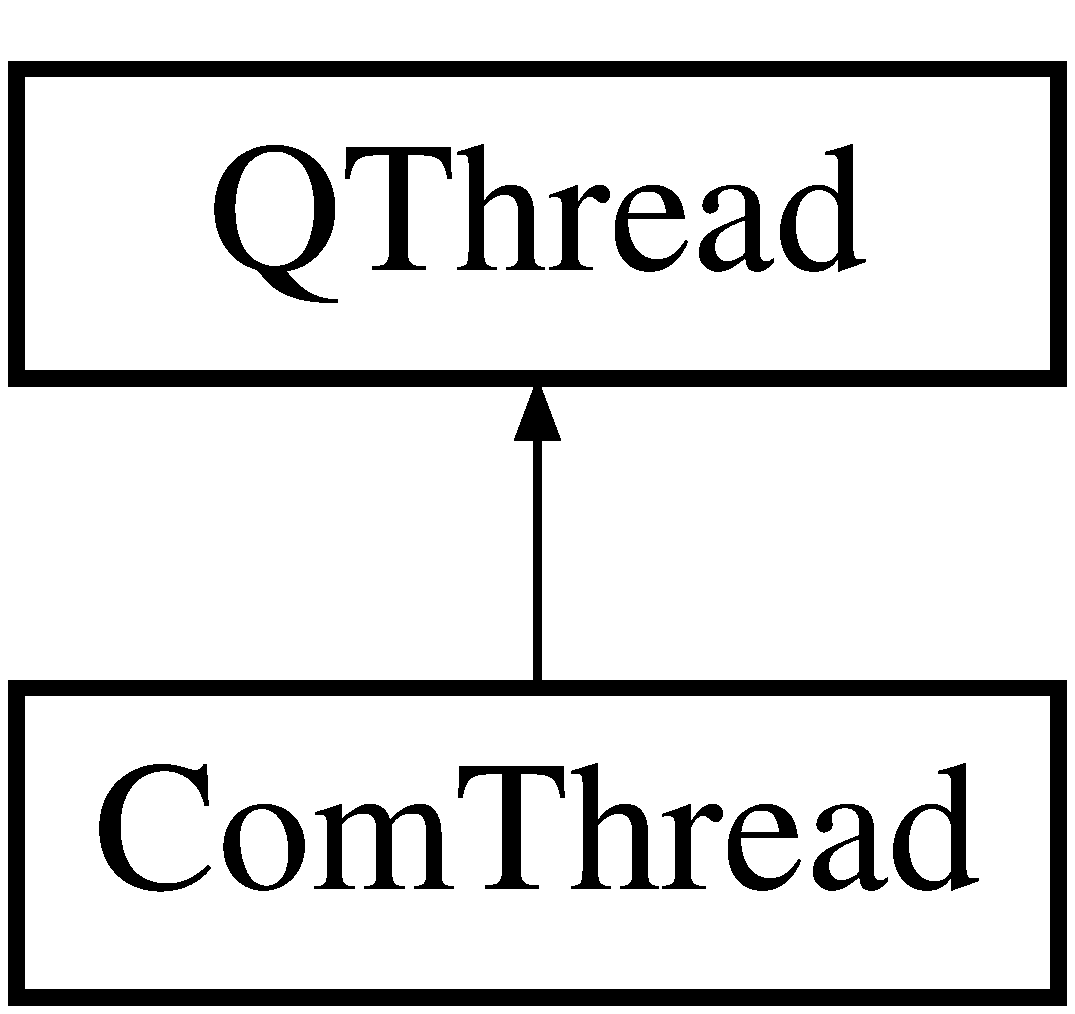
\includegraphics[height=2.000000cm]{d7/d46/a00002}
\end{center}
\end{figure}
\subsection*{Public Slots}
\subsection*{Signals}
\subsection*{Public Member Functions}
\subsection*{Private Attributes}


\subsection{Detailed Description}


\subsection{Constructor \& Destructor Documentation}
\hypertarget{a00002_ab24bebbd2ca81a9931aa0184366c9ba2}{\index{Com\-Thread@{Com\-Thread}!Com\-Thread@{Com\-Thread}}
\index{Com\-Thread@{Com\-Thread}!ComThread@{Com\-Thread}}
\subsubsection[{Com\-Thread}]{\setlength{\rightskip}{0pt plus 5cm}{\bf Com\-Thread} (
\begin{DoxyParamCaption}
{}
\end{DoxyParamCaption}
)}}\label{a00002_ab24bebbd2ca81a9931aa0184366c9ba2}


Constructor. 


\begin{DoxyParams}{Parameters}
{\em none} & \\
\hline
\end{DoxyParams}

\begin{DoxyExceptions}{Exceptions}
{\em none} & \\
\hline
\end{DoxyExceptions}
\begin{DoxyReturn}{Returns}
\hyperlink{a00002}{Com\-Thread} instance 
\end{DoxyReturn}

\begin{DoxyCode}
8 \{
9     \hyperlink{a00002_a07ff1fa563f3d58110ce80c3c1796f9b}{handle} = NULL;
10 
11     \hyperlink{a00002_a9954a8d34e6014302ae1d99cf5714cc9}{dcb}.DCBlength = \textcolor{keyword}{sizeof}(DCB);
12     \hyperlink{a00002_a9954a8d34e6014302ae1d99cf5714cc9}{dcb}.BaudRate = CBR\_57600;   \textcolor{comment}{/*  vitesse */}
13         \hyperlink{a00002_a9954a8d34e6014302ae1d99cf5714cc9}{dcb}.fBinary = \textcolor{keyword}{true};
14     \hyperlink{a00002_a9954a8d34e6014302ae1d99cf5714cc9}{dcb}.fParity = \textcolor{keyword}{false};
15     \hyperlink{a00002_a9954a8d34e6014302ae1d99cf5714cc9}{dcb}.fOutxCtsFlow = \textcolor{keyword}{false};
16     \hyperlink{a00002_a9954a8d34e6014302ae1d99cf5714cc9}{dcb}.fOutxDsrFlow = \textcolor{keyword}{false};
17     \hyperlink{a00002_a9954a8d34e6014302ae1d99cf5714cc9}{dcb}.fDtrControl = DTR\_CONTROL\_ENABLE;
18     \hyperlink{a00002_a9954a8d34e6014302ae1d99cf5714cc9}{dcb}.fDsrSensitivity = \textcolor{keyword}{false};
19     \hyperlink{a00002_a9954a8d34e6014302ae1d99cf5714cc9}{dcb}.fTXContinueOnXoff = \textcolor{keyword}{false};
20     \hyperlink{a00002_a9954a8d34e6014302ae1d99cf5714cc9}{dcb}.fOutX = \textcolor{keyword}{false};
21     \hyperlink{a00002_a9954a8d34e6014302ae1d99cf5714cc9}{dcb}.fInX = \textcolor{keyword}{false};
22     \hyperlink{a00002_a9954a8d34e6014302ae1d99cf5714cc9}{dcb}.fErrorChar = \textcolor{keyword}{false};
23     \hyperlink{a00002_a9954a8d34e6014302ae1d99cf5714cc9}{dcb}.fNull = \textcolor{keyword}{false};
24     \hyperlink{a00002_a9954a8d34e6014302ae1d99cf5714cc9}{dcb}.fRtsControl = RTS\_CONTROL\_ENABLE;
25     \hyperlink{a00002_a9954a8d34e6014302ae1d99cf5714cc9}{dcb}.fAbortOnError = \textcolor{keyword}{false};
26     \hyperlink{a00002_a9954a8d34e6014302ae1d99cf5714cc9}{dcb}.fDummy2 = 0;
27     \hyperlink{a00002_a9954a8d34e6014302ae1d99cf5714cc9}{dcb}.wReserved = 0;
28     \hyperlink{a00002_a9954a8d34e6014302ae1d99cf5714cc9}{dcb}.XonLim = 0x100;
29     \hyperlink{a00002_a9954a8d34e6014302ae1d99cf5714cc9}{dcb}.XoffLim = 0x100;
30     \hyperlink{a00002_a9954a8d34e6014302ae1d99cf5714cc9}{dcb}.ByteSize = 8 ; \textcolor{comment}{/* nombre de bits */}
31     \hyperlink{a00002_a9954a8d34e6014302ae1d99cf5714cc9}{dcb}.Parity = NOPARITY;
32     \hyperlink{a00002_a9954a8d34e6014302ae1d99cf5714cc9}{dcb}.StopBits = ONESTOPBIT;
33     \hyperlink{a00002_a9954a8d34e6014302ae1d99cf5714cc9}{dcb}.XonChar = 0x11;
34     \hyperlink{a00002_a9954a8d34e6014302ae1d99cf5714cc9}{dcb}.XoffChar = 0x13;
35     \hyperlink{a00002_a9954a8d34e6014302ae1d99cf5714cc9}{dcb}.ErrorChar = \textcolor{charliteral}{'?'};
36     \hyperlink{a00002_a9954a8d34e6014302ae1d99cf5714cc9}{dcb}.EofChar = 0x1a;
37     \hyperlink{a00002_a9954a8d34e6014302ae1d99cf5714cc9}{dcb}.EvtChar = 0x10;
38 
39     \hyperlink{a00002_a53794d9466be19cb9c0b65f87090e237}{failed} = \textcolor{keyword}{false};
40     \hyperlink{a00002_a8e19c465f25509158341edd459c119b1}{failNoticed} = \textcolor{keyword}{false};
41 \}
\end{DoxyCode}
\hypertarget{a00002_acbe0fd6d9516075ea60fb81b8a323461}{\index{Com\-Thread@{Com\-Thread}!$\sim$\-Com\-Thread@{$\sim$\-Com\-Thread}}
\index{$\sim$\-Com\-Thread@{$\sim$\-Com\-Thread}!ComThread@{Com\-Thread}}
\subsubsection[{$\sim$\-Com\-Thread}]{\setlength{\rightskip}{0pt plus 5cm}$\sim${\bf Com\-Thread} (
\begin{DoxyParamCaption}
{}
\end{DoxyParamCaption}
)}}\label{a00002_acbe0fd6d9516075ea60fb81b8a323461}


Destructor. 


\begin{DoxyParams}{Parameters}
{\em none} & \\
\hline
\end{DoxyParams}

\begin{DoxyExceptions}{Exceptions}
{\em none} & \\
\hline
\end{DoxyExceptions}
\begin{DoxyReturn}{Returns}
none 
\end{DoxyReturn}

\begin{DoxyCode}
44 \{
45 \}
\end{DoxyCode}


\subsection{Member Function Documentation}
\hypertarget{a00002_a34bd4298c27ce53379ec5eb23db83601}{\index{Com\-Thread@{Com\-Thread}!clear\-Counters@{clear\-Counters}}
\index{clear\-Counters@{clear\-Counters}!ComThread@{Com\-Thread}}
\subsubsection[{clear\-Counters}]{\setlength{\rightskip}{0pt plus 5cm}void clear\-Counters (
\begin{DoxyParamCaption}
{}
\end{DoxyParamCaption}
)}}\label{a00002_a34bd4298c27ce53379ec5eb23db83601}


Reset all counters. 


\begin{DoxyParams}{Parameters}
{\em none} & \\
\hline
\end{DoxyParams}

\begin{DoxyExceptions}{Exceptions}
{\em none} & \\
\hline
\end{DoxyExceptions}
\begin{DoxyReturn}{Returns}
none 
\end{DoxyReturn}

\begin{DoxyCode}
301 \{
302     \hyperlink{a00002_ad1e1c4a0c8bb235b5e26ec9c5d1c3f0d}{sizeWrite} = 0;
303     \hyperlink{a00002_ad9f5381795006f1f187538296368cd11}{sizeRead} = 0;
304     \hyperlink{a00002_a608be86b18e15c3309a1b50794a2115c}{sizePoll} = 0;
305 \}
\end{DoxyCode}
\hypertarget{a00002_a665582c4fbc3a48be815747e26dd6a02}{\index{Com\-Thread@{Com\-Thread}!create\-Com@{create\-Com}}
\index{create\-Com@{create\-Com}!ComThread@{Com\-Thread}}
\subsubsection[{create\-Com}]{\setlength{\rightskip}{0pt plus 5cm}void create\-Com (
\begin{DoxyParamCaption}
\item[{Q\-String}]{p\-\_\-s\-Com}
\end{DoxyParamCaption}
)}}\label{a00002_a665582c4fbc3a48be815747e26dd6a02}


Create the C\-O\-M port handler. 


\begin{DoxyParams}{Parameters}
{\em p\-\_\-s\-Com} & C\-O\-M port name Q\-String \\
\hline
\end{DoxyParams}

\begin{DoxyExceptions}{Exceptions}
{\em none} & \\
\hline
\end{DoxyExceptions}
\begin{DoxyReturn}{Returns}
none 
\end{DoxyReturn}

\begin{DoxyCode}
48 \{
49 
50 
51     \hyperlink{a00002_a07ff1fa563f3d58110ce80c3c1796f9b}{handle} = CreateFile((LPCWSTR)p\_sCom.constData(), GENERIC\_READ|GENERIC\_WRITE, 0, NULL, 
      OPEN\_EXISTING, FILE\_ATTRIBUTE\_SYSTEM, NULL);
52 
53     \textcolor{keywordflow}{if} (\hyperlink{a00002_a07ff1fa563f3d58110ce80c3c1796f9b}{handle} == INVALID\_HANDLE\_VALUE)
54     \{
55         \hyperlink{a00002_a07ff1fa563f3d58110ce80c3c1796f9b}{handle} = NULL;
56     \}
57     \textcolor{keywordflow}{else} \textcolor{keywordflow}{if} (\hyperlink{a00002_a53794d9466be19cb9c0b65f87090e237}{failed})
58     \{
59         emit \hyperlink{a00002_afb47495b5727dae0e7a5bac62098cb1e}{XBeeReconnected}();
60         \hyperlink{a00002_a8e19c465f25509158341edd459c119b1}{failNoticed} = \textcolor{keyword}{false};
61         \hyperlink{a00002_a53794d9466be19cb9c0b65f87090e237}{failed} = \textcolor{keyword}{false};
62     \}
63 
64     COMMTIMEOUTS g\_cto =
65     \{
66         READ\_INTERVAL,      \textcolor{comment}{/* ReadIntervalTimeOut          */}
67         READ\_MULTIPLIER,    \textcolor{comment}{/* ReadTotalTimeOutMultiplier   */}
68         MAX\_WAIT\_READ,      \textcolor{comment}{/* ReadTotalTimeOutConstant     */}
69         0,                  \textcolor{comment}{/* WriteTotalTimeOutMultiplier  */}
70         0                   \textcolor{comment}{/* WriteTotalTimeOutConstant    */}
71     \};
72 
73     SetupComm(\hyperlink{a00002_a07ff1fa563f3d58110ce80c3c1796f9b}{handle}, RX\_SIZE, TX\_SIZE);
74 
75     \textcolor{keywordflow}{if}(!SetCommTimeouts(\hyperlink{a00002_a07ff1fa563f3d58110ce80c3c1796f9b}{handle}, &g\_cto) || !SetCommState(\hyperlink{a00002_a07ff1fa563f3d58110ce80c3c1796f9b}{handle}, &
      \hyperlink{a00002_a9954a8d34e6014302ae1d99cf5714cc9}{dcb}))
76     \{
77         CloseHandle(\hyperlink{a00002_a07ff1fa563f3d58110ce80c3c1796f9b}{handle});
78         \hyperlink{a00002_a07ff1fa563f3d58110ce80c3c1796f9b}{handle} = NULL;
79     \}
80 
81     PurgeComm(\hyperlink{a00002_a07ff1fa563f3d58110ce80c3c1796f9b}{handle}, PURGE\_TXCLEAR|PURGE\_RXCLEAR|PURGE\_TXABORT|PURGE\_RXABORT);
82     EscapeCommFunction(\hyperlink{a00002_a07ff1fa563f3d58110ce80c3c1796f9b}{handle}, SETDTR);
83 
84 \}
\end{DoxyCode}
\hypertarget{a00002_a406892b365248cd6b35030378d1d4310}{\index{Com\-Thread@{Com\-Thread}!data\-Received@{data\-Received}}
\index{data\-Received@{data\-Received}!ComThread@{Com\-Thread}}
\subsubsection[{data\-Received}]{\setlength{\rightskip}{0pt plus 5cm}void data\-Received (
\begin{DoxyParamCaption}
\item[{char $\ast$}]{buffer, }
\item[{int}]{length}
\end{DoxyParamCaption}
)\hspace{0.3cm}{\ttfamily [signal]}}}\label{a00002_a406892b365248cd6b35030378d1d4310}


Data received event signal. 


\begin{DoxyParams}{Parameters}
{\em buffer} & reception buffer char$\ast$ \\
\hline
{\em length} & number of received char int \\
\hline
\end{DoxyParams}

\begin{DoxyExceptions}{Exceptions}
{\em none} & \\
\hline
\end{DoxyExceptions}
\begin{DoxyReturn}{Returns}
none 
\end{DoxyReturn}
\hypertarget{a00002_a8a8485f38f2aef24f1fd53c31949876b}{\index{Com\-Thread@{Com\-Thread}!poll@{poll}}
\index{poll@{poll}!ComThread@{Com\-Thread}}
\subsubsection[{poll}]{\setlength{\rightskip}{0pt plus 5cm}void poll (
\begin{DoxyParamCaption}
\item[{unsigned short}]{p\-Data\-To\-Poll}
\end{DoxyParamCaption}
)\hspace{0.3cm}{\ttfamily [slot]}}}\label{a00002_a8a8485f38f2aef24f1fd53c31949876b}


Poll data slot. 


\begin{DoxyParams}{Parameters}
{\em p\-Data\-To\-Poll} & data packet to poll descriptor unsigned short \\
\hline
\end{DoxyParams}

\begin{DoxyExceptions}{Exceptions}
{\em none} & \\
\hline
\end{DoxyExceptions}
\begin{DoxyReturn}{Returns}
none 
\end{DoxyReturn}

\begin{DoxyCode}
265 \{
266     memcpy((\textcolor{keywordtype}{void}*)\hyperlink{a00002_a581ac8ca710cda078fd8ddb8e50954eb}{dataToPoll}, \textcolor{stringliteral}{">*>p"}, 4);
267     memcpy((\textcolor{keywordtype}{void}*)&\hyperlink{a00002_a581ac8ca710cda078fd8ddb8e50954eb}{dataToPoll}[4], &pDataToPoll, \textcolor{keyword}{sizeof}(\textcolor{keywordtype}{short}));
268     \hyperlink{a00002_a608be86b18e15c3309a1b50794a2115c}{sizePoll} = 4 + \textcolor{keyword}{sizeof}(short);
269     \hyperlink{a00002_ad9f5381795006f1f187538296368cd11}{sizeRead} = 0;
270     \hyperlink{a00002_a21713484042dd9404528d9cec57ebe87}{mustPoll} = \textcolor{keyword}{true};
271 
272     \hyperlink{a00002_a129a62f35fc57084ceccbdc82794d9c1}{mustRead} = \textcolor{keyword}{true};
273 
274     \textcolor{keywordflow}{if} (pDataToPoll & STATUS\_PACKET)
275     \{
276         \hyperlink{a00002_ad9f5381795006f1f187538296368cd11}{sizeRead} += \textcolor{keyword}{sizeof}(\textcolor{stringliteral}{">*>"}) - 1 +  \textcolor{keyword}{sizeof}(\textcolor{keywordtype}{short}) + \textcolor{keyword}{sizeof}(char) + \textcolor{keyword}{sizeof}(
      \hyperlink{a00004_df/d98/a00107}{LL\_STATUS}) + \textcolor{keyword}{sizeof}(short) + \textcolor{keyword}{sizeof}(\textcolor{stringliteral}{"<#<"}) - 1;
277     \}
278 
279     \textcolor{keywordflow}{if} (pDataToPoll & GPS\_PACKET)
280     \{
281         \hyperlink{a00002_ad9f5381795006f1f187538296368cd11}{sizeRead} += \textcolor{keyword}{sizeof}(\textcolor{stringliteral}{">*>"}) - 1 +  \textcolor{keyword}{sizeof}(\textcolor{keywordtype}{short}) + \textcolor{keyword}{sizeof}(char) + \textcolor{keyword}{sizeof}(
      \hyperlink{a00004_d3/d32/a00105}{GPS\_DATA\_ADVANCED}) + \textcolor{keyword}{sizeof}(short) + \textcolor{keyword}{sizeof}(\textcolor{stringliteral}{"<#<"}) - 1;
282     \}
283 
284     \textcolor{keywordflow}{if} (pDataToPoll & CURRENT\_WAY\_PACKET)
285     \{
286         \hyperlink{a00002_ad9f5381795006f1f187538296368cd11}{sizeRead} += \textcolor{keyword}{sizeof}(\textcolor{stringliteral}{">*>"}) - 1 +  \textcolor{keyword}{sizeof}(\textcolor{keywordtype}{short}) + \textcolor{keyword}{sizeof}(char) + \textcolor{keyword}{sizeof}(
      \hyperlink{a00004_d1/d84/a00052}{CURRENT\_WAY}) + \textcolor{keyword}{sizeof}(short) + \textcolor{keyword}{sizeof}(\textcolor{stringliteral}{"<#<"}) - 1;
287     \}
288 
289     \textcolor{keywordflow}{if} (pDataToPoll & IMU\_CALCDATA\_PACKET)
290     \{
291         \hyperlink{a00002_ad9f5381795006f1f187538296368cd11}{sizeRead} += \textcolor{keyword}{sizeof}(\textcolor{stringliteral}{">*>"}) - 1 +  \textcolor{keyword}{sizeof}(\textcolor{keywordtype}{short}) + \textcolor{keyword}{sizeof}(char) + \textcolor{keyword}{sizeof}(
      \hyperlink{a00004_d7/d70/a00106}{IMU\_CALCDATA}) + \textcolor{keyword}{sizeof}(short) + \textcolor{keyword}{sizeof}(\textcolor{stringliteral}{"<#<"}) - 1;
292     \}
293 
294     \textcolor{keywordflow}{if} (pDataToPoll & RC\_DATA\_PACKET)
295     \{
296         \hyperlink{a00002_ad9f5381795006f1f187538296368cd11}{sizeRead} += \textcolor{keyword}{sizeof}(\textcolor{stringliteral}{">*>"}) - 1 +  \textcolor{keyword}{sizeof}(\textcolor{keywordtype}{short}) + \textcolor{keyword}{sizeof}(char) + \textcolor{keyword}{sizeof}(
      \hyperlink{a00004_d1/dd6/a00108}{RC\_DATA}) + \textcolor{keyword}{sizeof}(short) + \textcolor{keyword}{sizeof}(\textcolor{stringliteral}{"<#<"}) - 1;
297     \}
298 \}
\end{DoxyCode}
\hypertarget{a00002_a681ba4ec7299214b9bb86e660fe22701}{\index{Com\-Thread@{Com\-Thread}!release\-Com@{release\-Com}}
\index{release\-Com@{release\-Com}!ComThread@{Com\-Thread}}
\subsubsection[{release\-Com}]{\setlength{\rightskip}{0pt plus 5cm}void release\-Com (
\begin{DoxyParamCaption}
{}
\end{DoxyParamCaption}
)}}\label{a00002_a681ba4ec7299214b9bb86e660fe22701}


Destruct the C\-O\-M port handler. 


\begin{DoxyParams}{Parameters}
{\em none} & \\
\hline
\end{DoxyParams}

\begin{DoxyExceptions}{Exceptions}
{\em none} & \\
\hline
\end{DoxyExceptions}
\begin{DoxyReturn}{Returns}
none 
\end{DoxyReturn}

\begin{DoxyCode}
87 \{
88     CloseHandle(\hyperlink{a00002_a07ff1fa563f3d58110ce80c3c1796f9b}{handle});
89     \hyperlink{a00002_a07ff1fa563f3d58110ce80c3c1796f9b}{handle} = NULL;
90 \}
\end{DoxyCode}
\hypertarget{a00002_a13a43e6d814de94978c515cb084873b1}{\index{Com\-Thread@{Com\-Thread}!run@{run}}
\index{run@{run}!ComThread@{Com\-Thread}}
\subsubsection[{run}]{\setlength{\rightskip}{0pt plus 5cm}void run (
\begin{DoxyParamCaption}
{}
\end{DoxyParamCaption}
)}}\label{a00002_a13a43e6d814de94978c515cb084873b1}


Q\-Thread run override. 


\begin{DoxyParams}{Parameters}
{\em none} & \\
\hline
\end{DoxyParams}

\begin{DoxyExceptions}{Exceptions}
{\em none} & \\
\hline
\end{DoxyExceptions}
\begin{DoxyReturn}{Returns}
none 
\end{DoxyReturn}

\begin{DoxyCode}
93 \{
94     \hyperlink{a00003_a50e15ae51c87ae06ab29c8148cb5f36c}{DWORD} nbReceived = 0;
95     \hyperlink{a00003_a50e15ae51c87ae06ab29c8148cb5f36c}{DWORD} nbWritten = 0;
96     \hyperlink{a00002_ad1e1c4a0c8bb235b5e26ec9c5d1c3f0d}{sizeWrite} = 0;
97     \hyperlink{a00002_ad9f5381795006f1f187538296368cd11}{sizeRead} = 0;
98 
99     \textcolor{keywordflow}{while} (1)
100     \{
101         \textcolor{keywordflow}{if} (\hyperlink{a00002_a07ff1fa563f3d58110ce80c3c1796f9b}{handle} != NULL)
102         \{
103             \textcolor{keywordflow}{if} (\hyperlink{a00002_a951ec1a18196d806edaf6d3fb517a239}{mustWrite} == \textcolor{keyword}{true})
104             \{
105                 \textcolor{keywordflow}{if} (WriteFile(\hyperlink{a00002_a07ff1fa563f3d58110ce80c3c1796f9b}{handle}, \hyperlink{a00002_a8e3c3dbe1da8cc4b648ab2a6d7ddb7c5}{command}, \hyperlink{a00002_ad1e1c4a0c8bb235b5e26ec9c5d1c3f0d}{sizeWrite}, &nbWritten, NULL) == \textcolor{keyword}{true})
106                 \{
107                                         \hyperlink{a00002_a951ec1a18196d806edaf6d3fb517a239}{mustWrite} = \textcolor{keyword}{false};
108                 \}
109                 \textcolor{keywordflow}{else}
110                 \{
111                                         \hyperlink{a00002_a53794d9466be19cb9c0b65f87090e237}{failed} = \textcolor{keyword}{true};
112                 \}
113             \}
114 
115             \textcolor{keywordflow}{if} (\hyperlink{a00002_a21713484042dd9404528d9cec57ebe87}{mustPoll} == \textcolor{keyword}{true})
116             \{
117                 \textcolor{keywordflow}{if} (WriteFile(\hyperlink{a00002_a07ff1fa563f3d58110ce80c3c1796f9b}{handle}, \hyperlink{a00002_a581ac8ca710cda078fd8ddb8e50954eb}{dataToPoll}, \hyperlink{a00002_a608be86b18e15c3309a1b50794a2115c}{sizePoll}, &nbWritten, NULL) == \textcolor{keyword}{
      true})
118                 \{
119                                         \hyperlink{a00002_a21713484042dd9404528d9cec57ebe87}{mustPoll} = \textcolor{keyword}{false};
120                 \}
121                 \textcolor{keywordflow}{else}
122                 \{
123                                         \hyperlink{a00002_a53794d9466be19cb9c0b65f87090e237}{failed} = \textcolor{keyword}{true};
124                 \}
125             \}
126 
127             \textcolor{keywordflow}{if} (\hyperlink{a00002_a129a62f35fc57084ceccbdc82794d9c1}{mustRead} == \textcolor{keyword}{true})
128             \{
129                 \textcolor{keywordflow}{if} (ReadFile(\hyperlink{a00002_a07ff1fa563f3d58110ce80c3c1796f9b}{handle}, \hyperlink{a00002_a9bfec7969db289b67014513bcabba47f}{buffer}, \hyperlink{a00002_ad9f5381795006f1f187538296368cd11}{sizeRead}, &nbReceived, NULL) == \textcolor{keyword}{true})
130                 \{
131                     PurgeComm(\hyperlink{a00002_a07ff1fa563f3d58110ce80c3c1796f9b}{handle}, PURGE\_RXCLEAR);
132                     \hyperlink{a00002_ad9f5381795006f1f187538296368cd11}{sizeRead} = 0;
133                                         \hyperlink{a00002_a129a62f35fc57084ceccbdc82794d9c1}{mustRead} = \textcolor{keyword}{false};
134                 \}
135                 \textcolor{keywordflow}{else}
136                 \{
137                                         \hyperlink{a00002_a53794d9466be19cb9c0b65f87090e237}{failed} = \textcolor{keyword}{true};
138                 \}
139             \}
140 
141             \textcolor{keywordflow}{if} (nbReceived >= \hyperlink{a00002_ad9f5381795006f1f187538296368cd11}{sizeRead} && nbReceived != 0)
142             \{
143                 emit \hyperlink{a00002_a406892b365248cd6b35030378d1d4310}{dataReceived}(\hyperlink{a00002_a9bfec7969db289b67014513bcabba47f}{buffer}, nbReceived);
144                                 nbReceived = 0;
145             \}
146 
147             \textcolor{keywordflow}{if} (\hyperlink{a00002_a53794d9466be19cb9c0b65f87090e237}{failed} && !\hyperlink{a00002_a8e19c465f25509158341edd459c119b1}{failNoticed})
148             \{
149                 emit \hyperlink{a00002_a289c96805ddb1941fe330931d73321a0}{XBeeDisconnected}();
150                                 \hyperlink{a00002_a8e19c465f25509158341edd459c119b1}{failNoticed} = \textcolor{keyword}{true};
151             \}
152         \}
153         QThread::msleep(10);
154     \}
155 \}
\end{DoxyCode}
\hypertarget{a00002_a26c718e7e95e398ee9368434c23d0622}{\index{Com\-Thread@{Com\-Thread}!send\-Go\-To@{send\-Go\-To}}
\index{send\-Go\-To@{send\-Go\-To}!ComThread@{Com\-Thread}}
\subsubsection[{send\-Go\-To}]{\setlength{\rightskip}{0pt plus 5cm}void send\-Go\-To (
\begin{DoxyParamCaption}
{}
\end{DoxyParamCaption}
)\hspace{0.3cm}{\ttfamily [slot]}}}\label{a00002_a26c718e7e95e398ee9368434c23d0622}


Send go to order slot. 


\begin{DoxyParams}{Parameters}
{\em none} & \\
\hline
\end{DoxyParams}

\begin{DoxyExceptions}{Exceptions}
{\em none} & \\
\hline
\end{DoxyExceptions}
\begin{DoxyReturn}{Returns}
none 
\end{DoxyReturn}

\begin{DoxyCode}
188 \{
189     memcpy((\textcolor{keywordtype}{void}*)\hyperlink{a00002_a8e3c3dbe1da8cc4b648ab2a6d7ddb7c5}{command}, \textcolor{stringliteral}{">*>wg"}, \textcolor{keyword}{sizeof}(\textcolor{stringliteral}{">*>wg"}) - 1);
190     \hyperlink{a00002_ad1e1c4a0c8bb235b5e26ec9c5d1c3f0d}{sizeWrite} = \textcolor{keyword}{sizeof}(\textcolor{stringliteral}{">*>wg"}) - 1;
191     \hyperlink{a00002_a951ec1a18196d806edaf6d3fb517a239}{mustWrite} = \textcolor{keyword}{true};
192 
193     \hyperlink{a00002_a129a62f35fc57084ceccbdc82794d9c1}{mustRead} = \textcolor{keyword}{true};
194     \hyperlink{a00002_ad9f5381795006f1f187538296368cd11}{sizeRead} += 5;
195 \}
\end{DoxyCode}
\hypertarget{a00002_ac898a9141e335cfee3e6c9ebb6815411}{\index{Com\-Thread@{Com\-Thread}!send\-Home@{send\-Home}}
\index{send\-Home@{send\-Home}!ComThread@{Com\-Thread}}
\subsubsection[{send\-Home}]{\setlength{\rightskip}{0pt plus 5cm}void send\-Home (
\begin{DoxyParamCaption}
{}
\end{DoxyParamCaption}
)\hspace{0.3cm}{\ttfamily [slot]}}}\label{a00002_ac898a9141e335cfee3e6c9ebb6815411}


Send come home order slot. 


\begin{DoxyParams}{Parameters}
{\em none} & \\
\hline
\end{DoxyParams}

\begin{DoxyExceptions}{Exceptions}
{\em none} & \\
\hline
\end{DoxyExceptions}
\begin{DoxyReturn}{Returns}
none 
\end{DoxyReturn}

\begin{DoxyCode}
158 \{
159     memcpy((\textcolor{keywordtype}{void}*)\hyperlink{a00002_a8e3c3dbe1da8cc4b648ab2a6d7ddb7c5}{command}, \textcolor{stringliteral}{">*>wh"}, \textcolor{keyword}{sizeof}(\textcolor{stringliteral}{">*>wh"}) - 1);
160     \hyperlink{a00002_ad1e1c4a0c8bb235b5e26ec9c5d1c3f0d}{sizeWrite} = \textcolor{keyword}{sizeof}(\textcolor{stringliteral}{">*>wh"}) - 1;
161     \hyperlink{a00002_a951ec1a18196d806edaf6d3fb517a239}{mustWrite} = \textcolor{keyword}{true};
162 
163     \hyperlink{a00002_a129a62f35fc57084ceccbdc82794d9c1}{mustRead} = \textcolor{keyword}{true};
164     \hyperlink{a00002_ad9f5381795006f1f187538296368cd11}{sizeRead} += 5;
165 \}
\end{DoxyCode}
\hypertarget{a00002_a2664ee66ff3ea7ed8cdca604bce4be33}{\index{Com\-Thread@{Com\-Thread}!send\-Land@{send\-Land}}
\index{send\-Land@{send\-Land}!ComThread@{Com\-Thread}}
\subsubsection[{send\-Land}]{\setlength{\rightskip}{0pt plus 5cm}void send\-Land (
\begin{DoxyParamCaption}
{}
\end{DoxyParamCaption}
)\hspace{0.3cm}{\ttfamily [slot]}}}\label{a00002_a2664ee66ff3ea7ed8cdca604bce4be33}


Send land order slot. 


\begin{DoxyParams}{Parameters}
{\em none} & \\
\hline
\end{DoxyParams}

\begin{DoxyExceptions}{Exceptions}
{\em none} & \\
\hline
\end{DoxyExceptions}
\begin{DoxyReturn}{Returns}
none 
\end{DoxyReturn}

\begin{DoxyCode}
168 \{
169     memcpy((\textcolor{keywordtype}{void}*)\hyperlink{a00002_a8e3c3dbe1da8cc4b648ab2a6d7ddb7c5}{command}, \textcolor{stringliteral}{">*>we"}, \textcolor{keyword}{sizeof}(\textcolor{stringliteral}{">*>we"}) - 1);
170     \hyperlink{a00002_ad1e1c4a0c8bb235b5e26ec9c5d1c3f0d}{sizeWrite} = \textcolor{keyword}{sizeof}(\textcolor{stringliteral}{">*>we"}) - 1;
171     \hyperlink{a00002_a951ec1a18196d806edaf6d3fb517a239}{mustWrite} = \textcolor{keyword}{true};
172 
173     \hyperlink{a00002_a129a62f35fc57084ceccbdc82794d9c1}{mustRead} = \textcolor{keyword}{true};
174     \hyperlink{a00002_ad9f5381795006f1f187538296368cd11}{sizeRead} += 5;
175 \}
\end{DoxyCode}
\hypertarget{a00002_a38513372e1af4752cee2e2d046c98821}{\index{Com\-Thread@{Com\-Thread}!send\-Launch@{send\-Launch}}
\index{send\-Launch@{send\-Launch}!ComThread@{Com\-Thread}}
\subsubsection[{send\-Launch}]{\setlength{\rightskip}{0pt plus 5cm}void send\-Launch (
\begin{DoxyParamCaption}
{}
\end{DoxyParamCaption}
)\hspace{0.3cm}{\ttfamily [slot]}}}\label{a00002_a38513372e1af4752cee2e2d046c98821}


Send launch (define home) order slot. 


\begin{DoxyParams}{Parameters}
{\em none} & \\
\hline
\end{DoxyParams}

\begin{DoxyExceptions}{Exceptions}
{\em none} & \\
\hline
\end{DoxyExceptions}
\begin{DoxyReturn}{Returns}
none 
\end{DoxyReturn}

\begin{DoxyCode}
178 \{
179     memcpy((\textcolor{keywordtype}{void}*)\hyperlink{a00002_a8e3c3dbe1da8cc4b648ab2a6d7ddb7c5}{command}, \textcolor{stringliteral}{">*>wl"}, \textcolor{keyword}{sizeof}(\textcolor{stringliteral}{">*>wl"}) - 1);
180     \hyperlink{a00002_ad1e1c4a0c8bb235b5e26ec9c5d1c3f0d}{sizeWrite} = \textcolor{keyword}{sizeof}(\textcolor{stringliteral}{">*>wl"}) - 1;
181     \hyperlink{a00002_a951ec1a18196d806edaf6d3fb517a239}{mustWrite} = \textcolor{keyword}{true};
182 
183     \hyperlink{a00002_a129a62f35fc57084ceccbdc82794d9c1}{mustRead} = \textcolor{keyword}{true};
184     \hyperlink{a00002_ad9f5381795006f1f187538296368cd11}{sizeRead} += 5;
185 \}
\end{DoxyCode}
\hypertarget{a00002_a01a812308fc692593b9abcab86bf003d}{\index{Com\-Thread@{Com\-Thread}!send\-Mot\-Off@{send\-Mot\-Off}}
\index{send\-Mot\-Off@{send\-Mot\-Off}!ComThread@{Com\-Thread}}
\subsubsection[{send\-Mot\-Off}]{\setlength{\rightskip}{0pt plus 5cm}void send\-Mot\-Off (
\begin{DoxyParamCaption}
{}
\end{DoxyParamCaption}
)\hspace{0.3cm}{\ttfamily [slot]}}}\label{a00002_a01a812308fc692593b9abcab86bf003d}


Send stop engines order slot. 


\begin{DoxyParams}{Parameters}
{\em none} & \\
\hline
\end{DoxyParams}

\begin{DoxyExceptions}{Exceptions}
{\em none} & \\
\hline
\end{DoxyExceptions}
\begin{DoxyReturn}{Returns}
none 
\end{DoxyReturn}

\begin{DoxyCode}
254 \{
255     \textcolor{keywordtype}{unsigned} \textcolor{keywordtype}{char} value = 0;
256 
257     memcpy((\textcolor{keywordtype}{void}*)\hyperlink{a00002_a8e3c3dbe1da8cc4b648ab2a6d7ddb7c5}{command}, \textcolor{stringliteral}{">*>m"}, 4);
258     memcpy((\textcolor{keywordtype}{void}*)&\hyperlink{a00002_a8e3c3dbe1da8cc4b648ab2a6d7ddb7c5}{command}[4], &value, 1);
259     \hyperlink{a00002_ad1e1c4a0c8bb235b5e26ec9c5d1c3f0d}{sizeWrite} = 5;
260         \hyperlink{a00002_a951ec1a18196d806edaf6d3fb517a239}{mustWrite} = \textcolor{keyword}{true};
261 
262 \}
\end{DoxyCode}
\hypertarget{a00002_ad6b67904e4b30f5a26bef654f8a3c4a6}{\index{Com\-Thread@{Com\-Thread}!send\-Mot\-On@{send\-Mot\-On}}
\index{send\-Mot\-On@{send\-Mot\-On}!ComThread@{Com\-Thread}}
\subsubsection[{send\-Mot\-On}]{\setlength{\rightskip}{0pt plus 5cm}void send\-Mot\-On (
\begin{DoxyParamCaption}
{}
\end{DoxyParamCaption}
)\hspace{0.3cm}{\ttfamily [slot]}}}\label{a00002_ad6b67904e4b30f5a26bef654f8a3c4a6}


Send start engines order slot. 


\begin{DoxyParams}{Parameters}
{\em none} & \\
\hline
\end{DoxyParams}

\begin{DoxyExceptions}{Exceptions}
{\em none} & \\
\hline
\end{DoxyExceptions}
\begin{DoxyReturn}{Returns}
none 
\end{DoxyReturn}

\begin{DoxyCode}
245 \{
246     \textcolor{keywordtype}{unsigned} \textcolor{keywordtype}{char} value = 1;
247     memcpy((\textcolor{keywordtype}{void}*)\hyperlink{a00002_a8e3c3dbe1da8cc4b648ab2a6d7ddb7c5}{command}, \textcolor{stringliteral}{">*>m"}, 4);
248     memcpy((\textcolor{keywordtype}{void}*)&\hyperlink{a00002_a8e3c3dbe1da8cc4b648ab2a6d7ddb7c5}{command}[4], &value, 1);
249     \hyperlink{a00002_ad1e1c4a0c8bb235b5e26ec9c5d1c3f0d}{sizeWrite} = 5;
250         \hyperlink{a00002_a951ec1a18196d806edaf6d3fb517a239}{mustWrite} = \textcolor{keyword}{true};
251    \}
\end{DoxyCode}
\hypertarget{a00002_afeec69b8ef45da950fab78df4a1584e3}{\index{Com\-Thread@{Com\-Thread}!send\-Move@{send\-Move}}
\index{send\-Move@{send\-Move}!ComThread@{Com\-Thread}}
\subsubsection[{send\-Move}]{\setlength{\rightskip}{0pt plus 5cm}void send\-Move (
\begin{DoxyParamCaption}
\item[{double}]{x, }
\item[{double}]{y, }
\item[{double}]{z, }
\item[{double}]{yaw}
\end{DoxyParamCaption}
)\hspace{0.3cm}{\ttfamily [slot]}}}\label{a00002_afeec69b8ef45da950fab78df4a1584e3}


Send relative waypoint slot. 


\begin{DoxyParams}{Parameters}
{\em x} & x axe move reference double \\
\hline
{\em y} & y axe move reference double \\
\hline
{\em z} & z axe move reference double \\
\hline
{\em yaw} & heading reference double \\
\hline
\end{DoxyParams}

\begin{DoxyExceptions}{Exceptions}
{\em none} & \\
\hline
\end{DoxyExceptions}
\begin{DoxyReturn}{Returns}
none 
\end{DoxyReturn}

\begin{DoxyCode}
222 \{
223     \hyperlink{a00002_a0dff6629133ecc492d6b9ab44b60cb80}{wp}.\hyperlink{a00004_a66219f3f331762fb4a8d21c1f01d1105}{wp\_number} = 1;
224     \hyperlink{a00002_a0dff6629133ecc492d6b9ab44b60cb80}{wp}.\hyperlink{a00004_a702e933b2034a3d94950c39bfdcd3052}{pos\_acc} = 10000;
225     \hyperlink{a00002_a0dff6629133ecc492d6b9ab44b60cb80}{wp}.\hyperlink{a00004_a9e291d833ba33b59d6063a0cd586a86b}{time} = 0;
226     \hyperlink{a00002_a0dff6629133ecc492d6b9ab44b60cb80}{wp}.\hyperlink{a00004_a38184c087a13ec7e1b887656d9ccf848}{max\_speed} = 100;
227     \hyperlink{a00002_a0dff6629133ecc492d6b9ab44b60cb80}{wp}.\hyperlink{a00004_a78b61a2d452301b80cd56942bfc362e0}{properties} = WPPROP\_HEIGHTENABLED | WPPROP\_YAWENABLED | WPPROP\_AUTOMATICGOTO;
228     \hyperlink{a00002_a0dff6629133ecc492d6b9ab44b60cb80}{wp}.\hyperlink{a00004_a80c0944640e62d3ed6c5419c1bcc0c88}{X} = x * 1000;
229     \hyperlink{a00002_a0dff6629133ecc492d6b9ab44b60cb80}{wp}.\hyperlink{a00004_aa482c4cc86a24474e4fb19b5b5978778}{Y} = y * 1000;
230     \hyperlink{a00002_a0dff6629133ecc492d6b9ab44b60cb80}{wp}.\hyperlink{a00004_ad12fc34ce789bce6c8a05d8a17138534}{height} = z * 1000;
231     \hyperlink{a00002_a0dff6629133ecc492d6b9ab44b60cb80}{wp}.\hyperlink{a00004_a7d2cd970242d8b46e019dd7653588b30}{yaw} = yaw * 1000;
232     \hyperlink{a00002_a0dff6629133ecc492d6b9ab44b60cb80}{wp}.\hyperlink{a00004_a8191d25c9e9667de75b852aa1b3cd7b7}{chksum} = 0xAAAA + \hyperlink{a00002_a0dff6629133ecc492d6b9ab44b60cb80}{wp}.\hyperlink{a00004_a7d2cd970242d8b46e019dd7653588b30}{yaw} + \hyperlink{a00002_a0dff6629133ecc492d6b9ab44b60cb80}{wp}.\hyperlink{a00004_ad12fc34ce789bce6c8a05d8a17138534}{height} + \hyperlink{a00002_a0dff6629133ecc492d6b9ab44b60cb80}{wp}.\hyperlink{a00004_a9e291d833ba33b59d6063a0cd586a86b}{time} + 
      \hyperlink{a00002_a0dff6629133ecc492d6b9ab44b60cb80}{wp}.\hyperlink{a00004_a80c0944640e62d3ed6c5419c1bcc0c88}{X} + \hyperlink{a00002_a0dff6629133ecc492d6b9ab44b60cb80}{wp}.\hyperlink{a00004_aa482c4cc86a24474e4fb19b5b5978778}{Y} + \hyperlink{a00002_a0dff6629133ecc492d6b9ab44b60cb80}{wp}.\hyperlink{a00004_a38184c087a13ec7e1b887656d9ccf848}{max\_speed} + \hyperlink{a00002_a0dff6629133ecc492d6b9ab44b60cb80}{wp}.\hyperlink{a00004_a702e933b2034a3d94950c39bfdcd3052}{pos\_acc} + \hyperlink{a00002_a0dff6629133ecc492d6b9ab44b60cb80}{wp}.
      \hyperlink{a00004_a78b61a2d452301b80cd56942bfc362e0}{properties} + \hyperlink{a00002_a0dff6629133ecc492d6b9ab44b60cb80}{wp}.\hyperlink{a00004_a66219f3f331762fb4a8d21c1f01d1105}{wp\_number};
233 
234     memcpy((\textcolor{keywordtype}{void}*)\hyperlink{a00002_a8e3c3dbe1da8cc4b648ab2a6d7ddb7c5}{command}, \textcolor{stringliteral}{">*>ws"}, \textcolor{keyword}{sizeof}(\textcolor{stringliteral}{">*>ws"}) - 1);
235     memcpy((\textcolor{keywordtype}{void}*)&\hyperlink{a00002_a8e3c3dbe1da8cc4b648ab2a6d7ddb7c5}{command}[\hyperlink{a00002_ad1e1c4a0c8bb235b5e26ec9c5d1c3f0d}{sizeWrite}], &\hyperlink{a00002_a0dff6629133ecc492d6b9ab44b60cb80}{wp}, \textcolor{keyword}{sizeof}(\hyperlink{a00004_dd/d42/a00109}{WAYPOINT}));
236     sizeWrite = \textcolor{keyword}{sizeof}(\textcolor{stringliteral}{">*>ws"}) - 1;
237     sizeWrite += \textcolor{keyword}{sizeof}(\hyperlink{a00004_dd/d42/a00109}{WAYPOINT});
238     \hyperlink{a00002_a951ec1a18196d806edaf6d3fb517a239}{mustWrite} = \textcolor{keyword}{true};
239 
240     \hyperlink{a00002_a129a62f35fc57084ceccbdc82794d9c1}{mustRead} = \textcolor{keyword}{true};
241     \hyperlink{a00002_ad9f5381795006f1f187538296368cd11}{sizeRead} += 5;
242 \}
\end{DoxyCode}
\hypertarget{a00002_adbfad4ea4f6a7fbd059e2d8ec65f1539}{\index{Com\-Thread@{Com\-Thread}!send\-Waypoint@{send\-Waypoint}}
\index{send\-Waypoint@{send\-Waypoint}!ComThread@{Com\-Thread}}
\subsubsection[{send\-Waypoint}]{\setlength{\rightskip}{0pt plus 5cm}void send\-Waypoint (
\begin{DoxyParamCaption}
\item[{double}]{x, }
\item[{double}]{y, }
\item[{double}]{z, }
\item[{double}]{number}
\end{DoxyParamCaption}
)\hspace{0.3cm}{\ttfamily [slot]}}}\label{a00002_adbfad4ea4f6a7fbd059e2d8ec65f1539}


Send waypoint slot. 


\begin{DoxyParams}{Parameters}
{\em x} & longitude reference double \\
\hline
{\em y} & latitude reference double \\
\hline
{\em z} & altitude reference double \\
\hline
{\em number} & waypoint number double \\
\hline
\end{DoxyParams}

\begin{DoxyExceptions}{Exceptions}
{\em none} & \\
\hline
\end{DoxyExceptions}
\begin{DoxyReturn}{Returns}
none 
\end{DoxyReturn}

\begin{DoxyCode}
198 \{
199     \hyperlink{a00002_a0dff6629133ecc492d6b9ab44b60cb80}{wp}.\hyperlink{a00004_a66219f3f331762fb4a8d21c1f01d1105}{wp\_number} = number;
200     \hyperlink{a00002_a0dff6629133ecc492d6b9ab44b60cb80}{wp}.\hyperlink{a00004_a702e933b2034a3d94950c39bfdcd3052}{pos\_acc} = 10000;
201     \hyperlink{a00002_a0dff6629133ecc492d6b9ab44b60cb80}{wp}.\hyperlink{a00004_a9e291d833ba33b59d6063a0cd586a86b}{time} = 0;
202     \hyperlink{a00002_a0dff6629133ecc492d6b9ab44b60cb80}{wp}.\hyperlink{a00004_a38184c087a13ec7e1b887656d9ccf848}{max\_speed} = 100;
203     \hyperlink{a00002_a0dff6629133ecc492d6b9ab44b60cb80}{wp}.\hyperlink{a00004_a78b61a2d452301b80cd56942bfc362e0}{properties} = WPPROP\_ABSCOORDS | WPPROP\_HEIGHTENABLED | WPPROP\_YAWENABLED;
204     \hyperlink{a00002_a0dff6629133ecc492d6b9ab44b60cb80}{wp}.\hyperlink{a00004_a80c0944640e62d3ed6c5419c1bcc0c88}{X} = x * 10000000;
205     \hyperlink{a00002_a0dff6629133ecc492d6b9ab44b60cb80}{wp}.\hyperlink{a00004_aa482c4cc86a24474e4fb19b5b5978778}{Y} = y * 10000000;
206     \hyperlink{a00002_a0dff6629133ecc492d6b9ab44b60cb80}{wp}.\hyperlink{a00004_ad12fc34ce789bce6c8a05d8a17138534}{height} = z * 1000;
207     \hyperlink{a00002_a0dff6629133ecc492d6b9ab44b60cb80}{wp}.\hyperlink{a00004_a7d2cd970242d8b46e019dd7653588b30}{yaw} = 0;
208     \hyperlink{a00002_a0dff6629133ecc492d6b9ab44b60cb80}{wp}.\hyperlink{a00004_a8191d25c9e9667de75b852aa1b3cd7b7}{chksum} = 0xAAAA + \hyperlink{a00002_a0dff6629133ecc492d6b9ab44b60cb80}{wp}.\hyperlink{a00004_a7d2cd970242d8b46e019dd7653588b30}{yaw} + \hyperlink{a00002_a0dff6629133ecc492d6b9ab44b60cb80}{wp}.\hyperlink{a00004_ad12fc34ce789bce6c8a05d8a17138534}{height} + \hyperlink{a00002_a0dff6629133ecc492d6b9ab44b60cb80}{wp}.\hyperlink{a00004_a9e291d833ba33b59d6063a0cd586a86b}{time} + 
      \hyperlink{a00002_a0dff6629133ecc492d6b9ab44b60cb80}{wp}.\hyperlink{a00004_a80c0944640e62d3ed6c5419c1bcc0c88}{X} + \hyperlink{a00002_a0dff6629133ecc492d6b9ab44b60cb80}{wp}.\hyperlink{a00004_aa482c4cc86a24474e4fb19b5b5978778}{Y} + \hyperlink{a00002_a0dff6629133ecc492d6b9ab44b60cb80}{wp}.\hyperlink{a00004_a38184c087a13ec7e1b887656d9ccf848}{max\_speed} + \hyperlink{a00002_a0dff6629133ecc492d6b9ab44b60cb80}{wp}.\hyperlink{a00004_a702e933b2034a3d94950c39bfdcd3052}{pos\_acc} + \hyperlink{a00002_a0dff6629133ecc492d6b9ab44b60cb80}{wp}.
      \hyperlink{a00004_a78b61a2d452301b80cd56942bfc362e0}{properties} + \hyperlink{a00002_a0dff6629133ecc492d6b9ab44b60cb80}{wp}.\hyperlink{a00004_a66219f3f331762fb4a8d21c1f01d1105}{wp\_number};
209 
210     memcpy((\textcolor{keywordtype}{void}*)\hyperlink{a00002_a8e3c3dbe1da8cc4b648ab2a6d7ddb7c5}{command}, \textcolor{stringliteral}{">*>ws"}, \textcolor{keyword}{sizeof}(\textcolor{stringliteral}{">*>ws"}) - 1);
211     memcpy((\textcolor{keywordtype}{void}*)&\hyperlink{a00002_a8e3c3dbe1da8cc4b648ab2a6d7ddb7c5}{command}[\hyperlink{a00002_ad1e1c4a0c8bb235b5e26ec9c5d1c3f0d}{sizeWrite}], &\hyperlink{a00002_a0dff6629133ecc492d6b9ab44b60cb80}{wp}, \textcolor{keyword}{sizeof}(\hyperlink{a00004_dd/d42/a00109}{WAYPOINT}));
212     sizeWrite = \textcolor{keyword}{sizeof}(\textcolor{stringliteral}{">*>ws"}) - 1;
213     sizeWrite += \textcolor{keyword}{sizeof}(\hyperlink{a00004_dd/d42/a00109}{WAYPOINT});
214     \hyperlink{a00002_a951ec1a18196d806edaf6d3fb517a239}{mustWrite} = \textcolor{keyword}{true};
215 
216     \hyperlink{a00002_a129a62f35fc57084ceccbdc82794d9c1}{mustRead} = \textcolor{keyword}{true};
217     \hyperlink{a00002_ad9f5381795006f1f187538296368cd11}{sizeRead} += 5;
218     qDebug()<<\textcolor{stringliteral}{"send it "};
219 \}
\end{DoxyCode}
\hypertarget{a00002_a289c96805ddb1941fe330931d73321a0}{\index{Com\-Thread@{Com\-Thread}!X\-Bee\-Disconnected@{X\-Bee\-Disconnected}}
\index{X\-Bee\-Disconnected@{X\-Bee\-Disconnected}!ComThread@{Com\-Thread}}
\subsubsection[{X\-Bee\-Disconnected}]{\setlength{\rightskip}{0pt plus 5cm}void X\-Bee\-Disconnected (
\begin{DoxyParamCaption}
{}
\end{DoxyParamCaption}
)\hspace{0.3cm}{\ttfamily [signal]}}}\label{a00002_a289c96805ddb1941fe330931d73321a0}


X\-Bee physically disconnected. 


\begin{DoxyParams}{Parameters}
{\em none} & \\
\hline
\end{DoxyParams}

\begin{DoxyExceptions}{Exceptions}
{\em none} & \\
\hline
\end{DoxyExceptions}
\begin{DoxyReturn}{Returns}
none 
\end{DoxyReturn}
\hypertarget{a00002_afb47495b5727dae0e7a5bac62098cb1e}{\index{Com\-Thread@{Com\-Thread}!X\-Bee\-Reconnected@{X\-Bee\-Reconnected}}
\index{X\-Bee\-Reconnected@{X\-Bee\-Reconnected}!ComThread@{Com\-Thread}}
\subsubsection[{X\-Bee\-Reconnected}]{\setlength{\rightskip}{0pt plus 5cm}void X\-Bee\-Reconnected (
\begin{DoxyParamCaption}
{}
\end{DoxyParamCaption}
)\hspace{0.3cm}{\ttfamily [signal]}}}\label{a00002_afb47495b5727dae0e7a5bac62098cb1e}


X\-Bee physically reconnected. 


\begin{DoxyParams}{Parameters}
{\em none} & \\
\hline
\end{DoxyParams}

\begin{DoxyExceptions}{Exceptions}
{\em none} & \\
\hline
\end{DoxyExceptions}
\begin{DoxyReturn}{Returns}
none 
\end{DoxyReturn}


\subsection{Field Documentation}
\hypertarget{a00002_a9bfec7969db289b67014513bcabba47f}{\index{Com\-Thread@{Com\-Thread}!buffer@{buffer}}
\index{buffer@{buffer}!ComThread@{Com\-Thread}}
\subsubsection[{buffer}]{\setlength{\rightskip}{0pt plus 5cm}char buffer\mbox{[}R\-X\-\_\-\-S\-I\-Z\-E\mbox{]}\hspace{0.3cm}{\ttfamily [private]}}}\label{a00002_a9bfec7969db289b67014513bcabba47f}
\hypertarget{a00002_a8e3c3dbe1da8cc4b648ab2a6d7ddb7c5}{\index{Com\-Thread@{Com\-Thread}!command@{command}}
\index{command@{command}!ComThread@{Com\-Thread}}
\subsubsection[{command}]{\setlength{\rightskip}{0pt plus 5cm}char command\mbox{[}T\-X\-\_\-\-S\-I\-Z\-E\mbox{]}\hspace{0.3cm}{\ttfamily [private]}}}\label{a00002_a8e3c3dbe1da8cc4b648ab2a6d7ddb7c5}
\hypertarget{a00002_a581ac8ca710cda078fd8ddb8e50954eb}{\index{Com\-Thread@{Com\-Thread}!data\-To\-Poll@{data\-To\-Poll}}
\index{data\-To\-Poll@{data\-To\-Poll}!ComThread@{Com\-Thread}}
\subsubsection[{data\-To\-Poll}]{\setlength{\rightskip}{0pt plus 5cm}char data\-To\-Poll\mbox{[}10\mbox{]}\hspace{0.3cm}{\ttfamily [private]}}}\label{a00002_a581ac8ca710cda078fd8ddb8e50954eb}
\hypertarget{a00002_a9954a8d34e6014302ae1d99cf5714cc9}{\index{Com\-Thread@{Com\-Thread}!dcb@{dcb}}
\index{dcb@{dcb}!ComThread@{Com\-Thread}}
\subsubsection[{dcb}]{\setlength{\rightskip}{0pt plus 5cm}D\-C\-B dcb\hspace{0.3cm}{\ttfamily [private]}}}\label{a00002_a9954a8d34e6014302ae1d99cf5714cc9}
\hypertarget{a00002_a53794d9466be19cb9c0b65f87090e237}{\index{Com\-Thread@{Com\-Thread}!failed@{failed}}
\index{failed@{failed}!ComThread@{Com\-Thread}}
\subsubsection[{failed}]{\setlength{\rightskip}{0pt plus 5cm}bool failed\hspace{0.3cm}{\ttfamily [private]}}}\label{a00002_a53794d9466be19cb9c0b65f87090e237}
\hypertarget{a00002_a8e19c465f25509158341edd459c119b1}{\index{Com\-Thread@{Com\-Thread}!fail\-Noticed@{fail\-Noticed}}
\index{fail\-Noticed@{fail\-Noticed}!ComThread@{Com\-Thread}}
\subsubsection[{fail\-Noticed}]{\setlength{\rightskip}{0pt plus 5cm}bool fail\-Noticed\hspace{0.3cm}{\ttfamily [private]}}}\label{a00002_a8e19c465f25509158341edd459c119b1}
\hypertarget{a00002_a07ff1fa563f3d58110ce80c3c1796f9b}{\index{Com\-Thread@{Com\-Thread}!handle@{handle}}
\index{handle@{handle}!ComThread@{Com\-Thread}}
\subsubsection[{handle}]{\setlength{\rightskip}{0pt plus 5cm}H\-A\-N\-D\-L\-E handle\hspace{0.3cm}{\ttfamily [private]}}}\label{a00002_a07ff1fa563f3d58110ce80c3c1796f9b}
\hypertarget{a00002_a21713484042dd9404528d9cec57ebe87}{\index{Com\-Thread@{Com\-Thread}!must\-Poll@{must\-Poll}}
\index{must\-Poll@{must\-Poll}!ComThread@{Com\-Thread}}
\subsubsection[{must\-Poll}]{\setlength{\rightskip}{0pt plus 5cm}bool must\-Poll\hspace{0.3cm}{\ttfamily [private]}}}\label{a00002_a21713484042dd9404528d9cec57ebe87}
\hypertarget{a00002_a129a62f35fc57084ceccbdc82794d9c1}{\index{Com\-Thread@{Com\-Thread}!must\-Read@{must\-Read}}
\index{must\-Read@{must\-Read}!ComThread@{Com\-Thread}}
\subsubsection[{must\-Read}]{\setlength{\rightskip}{0pt plus 5cm}bool must\-Read\hspace{0.3cm}{\ttfamily [private]}}}\label{a00002_a129a62f35fc57084ceccbdc82794d9c1}
\hypertarget{a00002_a951ec1a18196d806edaf6d3fb517a239}{\index{Com\-Thread@{Com\-Thread}!must\-Write@{must\-Write}}
\index{must\-Write@{must\-Write}!ComThread@{Com\-Thread}}
\subsubsection[{must\-Write}]{\setlength{\rightskip}{0pt plus 5cm}bool must\-Write\hspace{0.3cm}{\ttfamily [private]}}}\label{a00002_a951ec1a18196d806edaf6d3fb517a239}
\hypertarget{a00002_a608be86b18e15c3309a1b50794a2115c}{\index{Com\-Thread@{Com\-Thread}!size\-Poll@{size\-Poll}}
\index{size\-Poll@{size\-Poll}!ComThread@{Com\-Thread}}
\subsubsection[{size\-Poll}]{\setlength{\rightskip}{0pt plus 5cm}int size\-Poll\hspace{0.3cm}{\ttfamily [private]}}}\label{a00002_a608be86b18e15c3309a1b50794a2115c}
\hypertarget{a00002_ad9f5381795006f1f187538296368cd11}{\index{Com\-Thread@{Com\-Thread}!size\-Read@{size\-Read}}
\index{size\-Read@{size\-Read}!ComThread@{Com\-Thread}}
\subsubsection[{size\-Read}]{\setlength{\rightskip}{0pt plus 5cm}unsigned long size\-Read\hspace{0.3cm}{\ttfamily [private]}}}\label{a00002_ad9f5381795006f1f187538296368cd11}
\hypertarget{a00002_ad1e1c4a0c8bb235b5e26ec9c5d1c3f0d}{\index{Com\-Thread@{Com\-Thread}!size\-Write@{size\-Write}}
\index{size\-Write@{size\-Write}!ComThread@{Com\-Thread}}
\subsubsection[{size\-Write}]{\setlength{\rightskip}{0pt plus 5cm}int size\-Write\hspace{0.3cm}{\ttfamily [private]}}}\label{a00002_ad1e1c4a0c8bb235b5e26ec9c5d1c3f0d}
\hypertarget{a00002_a578f5ec7742dce06b86799b36f1d138c}{\index{Com\-Thread@{Com\-Thread}!timer\-Fail@{timer\-Fail}}
\index{timer\-Fail@{timer\-Fail}!ComThread@{Com\-Thread}}
\subsubsection[{timer\-Fail}]{\setlength{\rightskip}{0pt plus 5cm}Q\-Timer timer\-Fail\hspace{0.3cm}{\ttfamily [private]}}}\label{a00002_a578f5ec7742dce06b86799b36f1d138c}
\hypertarget{a00002_a0dff6629133ecc492d6b9ab44b60cb80}{\index{Com\-Thread@{Com\-Thread}!wp@{wp}}
\index{wp@{wp}!ComThread@{Com\-Thread}}
\subsubsection[{wp}]{\setlength{\rightskip}{0pt plus 5cm}{\bf W\-A\-Y\-P\-O\-I\-N\-T} wp\hspace{0.3cm}{\ttfamily [private]}}}\label{a00002_a0dff6629133ecc492d6b9ab44b60cb80}


The documentation for this class was generated from the following files\-:\begin{DoxyCompactItemize}
\item 
\hyperlink{a00004}{Com\-Thread.\-h}\item 
\hyperlink{a00020}{Com\-Thread.\-cpp}\end{DoxyCompactItemize}

\hypertarget{a00005}{\section{Joystick\-Grabber Class Reference}
\label{a00005}\index{Joystick\-Grabber@{Joystick\-Grabber}}
}


{\ttfamily \#include \char`\"{}Joystick\-Grabber.\-h\char`\"{}}

Inheritance diagram for Joystick\-Grabber\-:\begin{figure}[H]
\begin{center}
\leavevmode
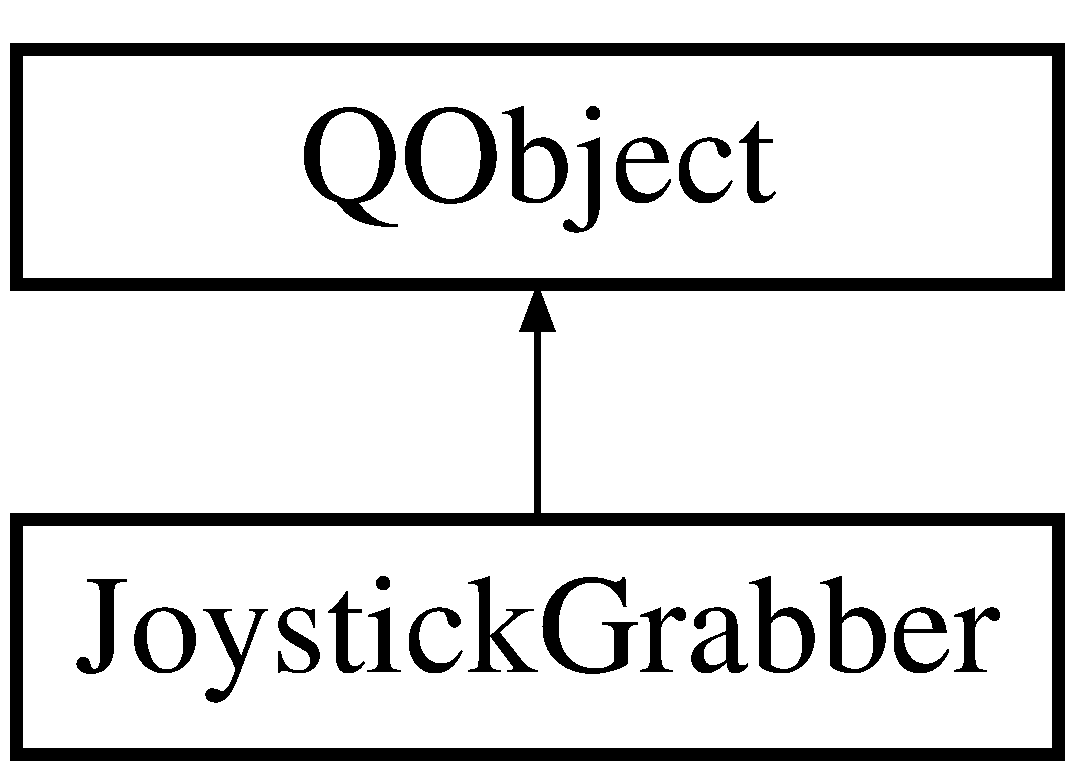
\includegraphics[height=2.000000cm]{dd/dad/a00005}
\end{center}
\end{figure}
\subsection*{Public Slots}
\subsection*{Signals}
\subsection*{Public Member Functions}
\subsection*{Data Fields}
\subsection*{Private Member Functions}
\subsection*{Private Attributes}


\subsection{Detailed Description}


\subsection{Constructor \& Destructor Documentation}
\hypertarget{a00005_a00527a60ea73ba28608e06e59dc9c638}{\index{Joystick\-Grabber@{Joystick\-Grabber}!Joystick\-Grabber@{Joystick\-Grabber}}
\index{Joystick\-Grabber@{Joystick\-Grabber}!JoystickGrabber@{Joystick\-Grabber}}
\subsubsection[{Joystick\-Grabber}]{\setlength{\rightskip}{0pt plus 5cm}{\bf Joystick\-Grabber} (
\begin{DoxyParamCaption}
{}
\end{DoxyParamCaption}
)}}\label{a00005_a00527a60ea73ba28608e06e59dc9c638}


Constructor. 


\begin{DoxyParams}{Parameters}
{\em none} & \\
\hline
\end{DoxyParams}

\begin{DoxyExceptions}{Exceptions}
{\em none} & \\
\hline
\end{DoxyExceptions}
\begin{DoxyReturn}{Returns}
\hyperlink{a00005}{Joystick\-Grabber} instance 
\end{DoxyReturn}

\begin{DoxyCode}
38 \{
39     \textcolor{comment}{/*}
40 \textcolor{comment}{    instance = GetModuleHandle(NULL);}
41 \textcolor{comment}{    m\_bDeviceNotCreated = true;}
42 \textcolor{comment}{    createDevice();}
43 \textcolor{comment}{}
44 \textcolor{comment}{    m\_bNoJoystick = false;}
45 \textcolor{comment}{    m\_bDirectInputProblem = false;}
46 \textcolor{comment}{    m\_bDataFormatProblem = false;}
47 \textcolor{comment}{    m\_bJoystickProblem = false;}
48 \textcolor{comment}{    m\_bDeviceEnumProblem = false;}
49 \textcolor{comment}{}
50 \textcolor{comment}{    connect(&m\_pTimer, SIGNAL(timeout()), SLOT(sendAcknowledge()));}
51 \textcolor{comment}{        */}
52 \}
\end{DoxyCode}


\subsection{Member Function Documentation}
\hypertarget{a00005_a7e8f5705bbae79af7d5c357280b9d17e}{\index{Joystick\-Grabber@{Joystick\-Grabber}!compute\-Data@{compute\-Data}}
\index{compute\-Data@{compute\-Data}!JoystickGrabber@{Joystick\-Grabber}}
\subsubsection[{compute\-Data}]{\setlength{\rightskip}{0pt plus 5cm}void compute\-Data (
\begin{DoxyParamCaption}
\item[{{\bf D\-I\-J\-O\-Y\-S\-T\-A\-T\-E}}]{state}
\end{DoxyParamCaption}
)\hspace{0.3cm}{\ttfamily [private]}}}\label{a00005_a7e8f5705bbae79af7d5c357280b9d17e}


Compute datat from game controller grab. 


\begin{DoxyParams}{Parameters}
{\em none} & \\
\hline
\end{DoxyParams}

\begin{DoxyExceptions}{Exceptions}
{\em none} & \\
\hline
\end{DoxyExceptions}
\begin{DoxyReturn}{Returns}
none 
\end{DoxyReturn}

\begin{DoxyCode}
112 \{
113     \textcolor{comment}{/*}
114 \textcolor{comment}{    leftStickX = (state.lX - 32767) / 32767.;}
115 \textcolor{comment}{    leftStickY = (state.lY - 32767) / 32767.;}
116 \textcolor{comment}{    topTrigger = (state.lZ - 32767) / 32767.;}
117 \textcolor{comment}{    rightStickX = (state.lRx - 32767) / 32767.;}
118 \textcolor{comment}{    rightStickY = (state.lRy - 32767) / 32767.;}
119 \textcolor{comment}{}
120 \textcolor{comment}{    for (int i = 0; i < 32; i++)}
121 \textcolor{comment}{    \{}
122 \textcolor{comment}{        buttons[i] = (state.rgbButtons[i] != 0);}
123 \textcolor{comment}{    \}}
124 \textcolor{comment}{}
125 \textcolor{comment}{    for (int i = 0; i < 4; i++)}
126 \textcolor{comment}{    \{}
127 \textcolor{comment}{        pov[i] = (state.rgdwPOV[i] != -1);}
128 \textcolor{comment}{    \}}
129 \textcolor{comment}{}
130 \textcolor{comment}{    emit dataComputed();}
131 \textcolor{comment}{        */}
132 \}
\end{DoxyCode}
\hypertarget{a00005_a2dfbfa6847025eb5bff311a5cdd23128}{\index{Joystick\-Grabber@{Joystick\-Grabber}!create\-Device@{create\-Device}}
\index{create\-Device@{create\-Device}!JoystickGrabber@{Joystick\-Grabber}}
\subsubsection[{create\-Device}]{\setlength{\rightskip}{0pt plus 5cm}void create\-Device (
\begin{DoxyParamCaption}
{}
\end{DoxyParamCaption}
)}}\label{a00005_a2dfbfa6847025eb5bff311a5cdd23128}


Create the Direct X device. 


\begin{DoxyParams}{Parameters}
{\em none} & \\
\hline
\end{DoxyParams}

\begin{DoxyExceptions}{Exceptions}
{\em none} & \\
\hline
\end{DoxyExceptions}
\begin{DoxyReturn}{Returns}
none 
\end{DoxyReturn}

\begin{DoxyCode}
55 \{
56     \textcolor{comment}{/*}
57 \textcolor{comment}{    //DirectInput object creation}
58 \textcolor{comment}{    result = DirectInput8Create(instance, DIRECTINPUT\_VERSION, IID\_IDirectInput8, (void**
      )&direct\_input\_object, NULL); }
59 \textcolor{comment}{}
60 \textcolor{comment}{    //Error management}
61 \textcolor{comment}{    if(FAILED(result))}
62 \textcolor{comment}{    \{}
63 \textcolor{comment}{        //Cannot create instance}
64 \textcolor{comment}{        //Possible errors : DIERR\_BETADIRECTINPUTVERSION, DIERR\_INVALIDPARAM, DIERR\_OLDDIRECTINPUTVERSION,
       DIERR\_OUTOFMEMORY}
65 \textcolor{comment}{        m\_bDirectInputProblem = true;}
66 \textcolor{comment}{        return;}
67 \textcolor{comment}{    \}}
68 \textcolor{comment}{}
69 \textcolor{comment}{    m\_bDirectInputProblem = false;}
70 \textcolor{comment}{}
71 \textcolor{comment}{    //Enumerate peripherals}
72 \textcolor{comment}{    result  = direct\_input\_object->EnumDevices(DI8DEVCLASS\_GAMECTRL, &CreateDeviceCallback, NULL,
       DIEDFL\_ATTACHEDONLY);}
73 \textcolor{comment}{}
74 \textcolor{comment}{    //Error management}
75 \textcolor{comment}{    if(FAILED(result))}
76 \textcolor{comment}{    \{}
77 \textcolor{comment}{        //Cannot create joypad}
78 \textcolor{comment}{        //possible errors : DIERR\_INVALIDPARAM, DIERR\_NOTINITIALIZED}
79 \textcolor{comment}{        m\_bDeviceEnumProblem = true;}
80 \textcolor{comment}{        return;}
81 \textcolor{comment}{    \}}
82 \textcolor{comment}{    m\_bDeviceEnumProblem = false;}
83 \textcolor{comment}{}
84 \textcolor{comment}{    if (joypad)}
85 \textcolor{comment}{    \{}
86 \textcolor{comment}{        //Data format used definition}
87 \textcolor{comment}{        result = joypad->SetDataFormat(&c\_dfDIJoystick); }
88 \textcolor{comment}{}
89 \textcolor{comment}{        //Error management}
90 \textcolor{comment}{        if(FAILED(result))}
91 \textcolor{comment}{        \{ }
92 \textcolor{comment}{            //Cannot initialize data format}
93 \textcolor{comment}{            //Possible errors : DIERR\_ACQUIRED, DIERR\_INVALIDPARAM, DIERR\_NOTINITIALIZED}
94 \textcolor{comment}{            m\_bDataFormatProblem = true;}
95 \textcolor{comment}{            return;}
96 \textcolor{comment}{        \}}
97 \textcolor{comment}{}
98 \textcolor{comment}{        m\_bDataFormatProblem = false;}
99 \textcolor{comment}{        m\_bNoJoystick = false;}
100 \textcolor{comment}{        m\_bDeviceNotCreated = false;}
101 \textcolor{comment}{}
102 \textcolor{comment}{        joypad->Acquire();}
103 \textcolor{comment}{    \}}
104 \textcolor{comment}{    else}
105 \textcolor{comment}{    \{}
106 \textcolor{comment}{        m\_bNoJoystick = true;}
107 \textcolor{comment}{    \}}
108 \textcolor{comment}{        */}
109 \}
\end{DoxyCode}
\hypertarget{a00005_a05f4229ff68c39c5983aa630a0ee359d}{\index{Joystick\-Grabber@{Joystick\-Grabber}!data\-Computed@{data\-Computed}}
\index{data\-Computed@{data\-Computed}!JoystickGrabber@{Joystick\-Grabber}}
\subsubsection[{data\-Computed}]{\setlength{\rightskip}{0pt plus 5cm}void data\-Computed (
\begin{DoxyParamCaption}
{}
\end{DoxyParamCaption}
)\hspace{0.3cm}{\ttfamily [signal]}}}\label{a00005_a05f4229ff68c39c5983aa630a0ee359d}


Data computed signal. 


\begin{DoxyParams}{Parameters}
{\em none} & \\
\hline
\end{DoxyParams}

\begin{DoxyExceptions}{Exceptions}
{\em none} & \\
\hline
\end{DoxyExceptions}
\begin{DoxyReturn}{Returns}
none 
\end{DoxyReturn}
\hypertarget{a00005_aa6bfaa413ce18461ac71e75248460700}{\index{Joystick\-Grabber@{Joystick\-Grabber}!data\-Format\-Problem@{data\-Format\-Problem}}
\index{data\-Format\-Problem@{data\-Format\-Problem}!JoystickGrabber@{Joystick\-Grabber}}
\subsubsection[{data\-Format\-Problem}]{\setlength{\rightskip}{0pt plus 5cm}void data\-Format\-Problem (
\begin{DoxyParamCaption}
{}
\end{DoxyParamCaption}
)\hspace{0.3cm}{\ttfamily [signal]}}}\label{a00005_aa6bfaa413ce18461ac71e75248460700}


Data format for controller problem signal. 


\begin{DoxyParams}{Parameters}
{\em none} & \\
\hline
\end{DoxyParams}

\begin{DoxyExceptions}{Exceptions}
{\em none} & \\
\hline
\end{DoxyExceptions}
\begin{DoxyReturn}{Returns}
none 
\end{DoxyReturn}
\hypertarget{a00005_a51a5a6418d902f49aa198a8d3ae923f6}{\index{Joystick\-Grabber@{Joystick\-Grabber}!device\-Enum\-Problem@{device\-Enum\-Problem}}
\index{device\-Enum\-Problem@{device\-Enum\-Problem}!JoystickGrabber@{Joystick\-Grabber}}
\subsubsection[{device\-Enum\-Problem}]{\setlength{\rightskip}{0pt plus 5cm}void device\-Enum\-Problem (
\begin{DoxyParamCaption}
{}
\end{DoxyParamCaption}
)\hspace{0.3cm}{\ttfamily [signal]}}}\label{a00005_a51a5a6418d902f49aa198a8d3ae923f6}


Enumeration of devices problem signal. 


\begin{DoxyParams}{Parameters}
{\em none} & \\
\hline
\end{DoxyParams}

\begin{DoxyExceptions}{Exceptions}
{\em none} & \\
\hline
\end{DoxyExceptions}
\begin{DoxyReturn}{Returns}
none 
\end{DoxyReturn}
\hypertarget{a00005_a10733eb4d9bf54f33699a23fe0e0c4f8}{\index{Joystick\-Grabber@{Joystick\-Grabber}!direct\-Input\-Problem@{direct\-Input\-Problem}}
\index{direct\-Input\-Problem@{direct\-Input\-Problem}!JoystickGrabber@{Joystick\-Grabber}}
\subsubsection[{direct\-Input\-Problem}]{\setlength{\rightskip}{0pt plus 5cm}void direct\-Input\-Problem (
\begin{DoxyParamCaption}
{}
\end{DoxyParamCaption}
)\hspace{0.3cm}{\ttfamily [signal]}}}\label{a00005_a10733eb4d9bf54f33699a23fe0e0c4f8}


Direct Input problem signal. 


\begin{DoxyParams}{Parameters}
{\em none} & \\
\hline
\end{DoxyParams}

\begin{DoxyExceptions}{Exceptions}
{\em none} & \\
\hline
\end{DoxyExceptions}
\begin{DoxyReturn}{Returns}
none 
\end{DoxyReturn}
\hypertarget{a00005_a8fee61d7a783cade1a3d07fe86284d27}{\index{Joystick\-Grabber@{Joystick\-Grabber}!Finalize@{Finalize}}
\index{Finalize@{Finalize}!JoystickGrabber@{Joystick\-Grabber}}
\subsubsection[{Finalize}]{\setlength{\rightskip}{0pt plus 5cm}void Finalize (
\begin{DoxyParamCaption}
\item[{void}]{}
\end{DoxyParamCaption}
)\hspace{0.3cm}{\ttfamily [private]}}}\label{a00005_a8fee61d7a783cade1a3d07fe86284d27}


Finalize the game controller handle. 


\begin{DoxyParams}{Parameters}
{\em none} & \\
\hline
\end{DoxyParams}

\begin{DoxyExceptions}{Exceptions}
{\em none} & \\
\hline
\end{DoxyExceptions}
\begin{DoxyReturn}{Returns}
none 
\end{DoxyReturn}

\begin{DoxyCode}
135 \{
136     \textcolor{comment}{/*}
137 \textcolor{comment}{    if (direct\_input\_object) }
138 \textcolor{comment}{    \{ }
139 \textcolor{comment}{        //Finalize peripheral}
140 \textcolor{comment}{        if (joypad) }
141 \textcolor{comment}{        \{ }
142 \textcolor{comment}{            joypad->Unacquire(); }
143 \textcolor{comment}{            joypad->Release();}
144 \textcolor{comment}{            joypad = NULL; }
145 \textcolor{comment}{        \} }
146 \textcolor{comment}{}
147 \textcolor{comment}{        //Finalize DirectInput}
148 \textcolor{comment}{        direct\_input\_object->Release();}
149 \textcolor{comment}{        direct\_input\_object = NULL; }
150 \textcolor{comment}{    \}}
151 \textcolor{comment}{        */}
152 \}
\end{DoxyCode}
\hypertarget{a00005_ae8d92c6f646a05d37cdee939fdc6110f}{\index{Joystick\-Grabber@{Joystick\-Grabber}!grab@{grab}}
\index{grab@{grab}!JoystickGrabber@{Joystick\-Grabber}}
\subsubsection[{grab}]{\setlength{\rightskip}{0pt plus 5cm}void grab (
\begin{DoxyParamCaption}
{}
\end{DoxyParamCaption}
)\hspace{0.3cm}{\ttfamily [slot]}}}\label{a00005_ae8d92c6f646a05d37cdee939fdc6110f}


Grab information one time. 


\begin{DoxyParams}{Parameters}
{\em none} & \\
\hline
\end{DoxyParams}

\begin{DoxyExceptions}{Exceptions}
{\em none} & \\
\hline
\end{DoxyExceptions}
\begin{DoxyReturn}{Returns}
none 
\end{DoxyReturn}

\begin{DoxyCode}
155 \{
156     \textcolor{comment}{/*}
157 \textcolor{comment}{    if (m\_pTimer.isActive() == false)}
158 \textcolor{comment}{    \{}
159 \textcolor{comment}{        m\_pTimer.start(300);}
160 \textcolor{comment}{    \}}
161 \textcolor{comment}{}
162 \textcolor{comment}{    if (m\_bDeviceNotCreated)}
163 \textcolor{comment}{    \{}
164 \textcolor{comment}{        createDevice();}
165 \textcolor{comment}{    \}}
166 \textcolor{comment}{}
167 \textcolor{comment}{    if (m\_bDeviceNotCreated == false)}
168 \textcolor{comment}{    \{}
169 \textcolor{comment}{        result = joypad->Poll(); }
170 \textcolor{comment}{}
171 \textcolor{comment}{        //Error management}
172 \textcolor{comment}{        if(FAILED(result))}
173 \textcolor{comment}{        \{ }
174 \textcolor{comment}{            m\_bDeviceNotCreated = true;}
175 \textcolor{comment}{            m\_bJoystickProblem = true;}
176 \textcolor{comment}{            return;}
177 \textcolor{comment}{        \}}
178 \textcolor{comment}{}
179 \textcolor{comment}{        result = joypad->GetDeviceState(sizeof(state), (LPVOID)&state); }
180 \textcolor{comment}{}
181 \textcolor{comment}{        //Error management}
182 \textcolor{comment}{        if(FAILED(result))}
183 \textcolor{comment}{        \{ }
184 \textcolor{comment}{            //Cannot get device state}
185 \textcolor{comment}{            //Possible errors : DIERR\_INPUTLOST, DIERR\_INVALIDPARAM, DIERR\_NOTACQUIRED,
       DIERR\_NOTINITIALIZED, E\_PENDING}
186 \textcolor{comment}{            m\_bJoystickProblem = true;}
187 \textcolor{comment}{            return;}
188 \textcolor{comment}{        \}}
189 \textcolor{comment}{        }
190 \textcolor{comment}{        m\_bJoystickProblem = false;}
191 \textcolor{comment}{        computeData(state);}
192 \textcolor{comment}{    \}}
193 \textcolor{comment}{        */}
194 \}
\end{DoxyCode}
\hypertarget{a00005_a2359b3e182aa100a1c8da8c5d05155fe}{\index{Joystick\-Grabber@{Joystick\-Grabber}!joystick\-Problem@{joystick\-Problem}}
\index{joystick\-Problem@{joystick\-Problem}!JoystickGrabber@{Joystick\-Grabber}}
\subsubsection[{joystick\-Problem}]{\setlength{\rightskip}{0pt plus 5cm}void joystick\-Problem (
\begin{DoxyParamCaption}
{}
\end{DoxyParamCaption}
)\hspace{0.3cm}{\ttfamily [signal]}}}\label{a00005_a2359b3e182aa100a1c8da8c5d05155fe}


Joystick access problem signal. 


\begin{DoxyParams}{Parameters}
{\em none} & \\
\hline
\end{DoxyParams}

\begin{DoxyExceptions}{Exceptions}
{\em none} & \\
\hline
\end{DoxyExceptions}
\begin{DoxyReturn}{Returns}
none 
\end{DoxyReturn}
\hypertarget{a00005_ad70a13ae9071262fc324babf6254d6ea}{\index{Joystick\-Grabber@{Joystick\-Grabber}!no\-Joystick@{no\-Joystick}}
\index{no\-Joystick@{no\-Joystick}!JoystickGrabber@{Joystick\-Grabber}}
\subsubsection[{no\-Joystick}]{\setlength{\rightskip}{0pt plus 5cm}void no\-Joystick (
\begin{DoxyParamCaption}
{}
\end{DoxyParamCaption}
)\hspace{0.3cm}{\ttfamily [signal]}}}\label{a00005_ad70a13ae9071262fc324babf6254d6ea}


No joystick or gamepad connected signal. 


\begin{DoxyParams}{Parameters}
{\em none} & \\
\hline
\end{DoxyParams}

\begin{DoxyExceptions}{Exceptions}
{\em none} & \\
\hline
\end{DoxyExceptions}
\begin{DoxyReturn}{Returns}
none 
\end{DoxyReturn}
\hypertarget{a00005_a6a2caa19e313a28cc345be6dd67f2121}{\index{Joystick\-Grabber@{Joystick\-Grabber}!send\-Acknowledge@{send\-Acknowledge}}
\index{send\-Acknowledge@{send\-Acknowledge}!JoystickGrabber@{Joystick\-Grabber}}
\subsubsection[{send\-Acknowledge}]{\setlength{\rightskip}{0pt plus 5cm}void send\-Acknowledge (
\begin{DoxyParamCaption}
{}
\end{DoxyParamCaption}
)\hspace{0.3cm}{\ttfamily [slot]}}}\label{a00005_a6a2caa19e313a28cc345be6dd67f2121}


Send errors each time interval of the timer. 


\begin{DoxyParams}{Parameters}
{\em none} & \\
\hline
\end{DoxyParams}

\begin{DoxyExceptions}{Exceptions}
{\em none} & \\
\hline
\end{DoxyExceptions}
\begin{DoxyReturn}{Returns}
none 
\end{DoxyReturn}

\begin{DoxyCode}
197 \{
198     \textcolor{comment}{/*}
199 \textcolor{comment}{    if (m\_bNoJoystick)}
200 \textcolor{comment}{    \{}
201 \textcolor{comment}{        emit noJoystick();}
202 \textcolor{comment}{    \}}
203 \textcolor{comment}{}
204 \textcolor{comment}{    if (m\_bDirectInputProblem)}
205 \textcolor{comment}{    \{}
206 \textcolor{comment}{        emit directInputProblem();}
207 \textcolor{comment}{    \}}
208 \textcolor{comment}{}
209 \textcolor{comment}{    if (m\_bDataFormatProblem)}
210 \textcolor{comment}{    \{}
211 \textcolor{comment}{        emit dataFormatProblem();}
212 \textcolor{comment}{    \}}
213 \textcolor{comment}{}
214 \textcolor{comment}{    if (m\_bJoystickProblem)}
215 \textcolor{comment}{    \{}
216 \textcolor{comment}{        emit joystickProblem();}
217 \textcolor{comment}{    \}}
218 \textcolor{comment}{}
219 \textcolor{comment}{    if (m\_bDeviceEnumProblem)}
220 \textcolor{comment}{    \{}
221 \textcolor{comment}{        emit deviceEnumProblem();}
222 \textcolor{comment}{    \}}
223 \textcolor{comment}{}
224 \textcolor{comment}{        */}
225 \}
\end{DoxyCode}


\subsection{Field Documentation}
\hypertarget{a00005_a79f4acbf0893aed36f0bf600410b9fde}{\index{Joystick\-Grabber@{Joystick\-Grabber}!buttons@{buttons}}
\index{buttons@{buttons}!JoystickGrabber@{Joystick\-Grabber}}
\subsubsection[{buttons}]{\setlength{\rightskip}{0pt plus 5cm}bool buttons\mbox{[}32\mbox{]}}}\label{a00005_a79f4acbf0893aed36f0bf600410b9fde}
\hypertarget{a00005_ab182c34f8588348767de30e37ac6c659}{\index{Joystick\-Grabber@{Joystick\-Grabber}!left\-Stick\-X@{left\-Stick\-X}}
\index{left\-Stick\-X@{left\-Stick\-X}!JoystickGrabber@{Joystick\-Grabber}}
\subsubsection[{left\-Stick\-X}]{\setlength{\rightskip}{0pt plus 5cm}double left\-Stick\-X}}\label{a00005_ab182c34f8588348767de30e37ac6c659}
\hypertarget{a00005_a3db012f463d24f44cefdfef69c495a0e}{\index{Joystick\-Grabber@{Joystick\-Grabber}!left\-Stick\-Y@{left\-Stick\-Y}}
\index{left\-Stick\-Y@{left\-Stick\-Y}!JoystickGrabber@{Joystick\-Grabber}}
\subsubsection[{left\-Stick\-Y}]{\setlength{\rightskip}{0pt plus 5cm}double left\-Stick\-Y}}\label{a00005_a3db012f463d24f44cefdfef69c495a0e}
\hypertarget{a00005_ace877f18c922f37da48234f6256cad3e}{\index{Joystick\-Grabber@{Joystick\-Grabber}!m\-\_\-b\-Data\-Format\-Problem@{m\-\_\-b\-Data\-Format\-Problem}}
\index{m\-\_\-b\-Data\-Format\-Problem@{m\-\_\-b\-Data\-Format\-Problem}!JoystickGrabber@{Joystick\-Grabber}}
\subsubsection[{m\-\_\-b\-Data\-Format\-Problem}]{\setlength{\rightskip}{0pt plus 5cm}bool m\-\_\-b\-Data\-Format\-Problem\hspace{0.3cm}{\ttfamily [private]}}}\label{a00005_ace877f18c922f37da48234f6256cad3e}
\hypertarget{a00005_aa8af7ff7c29595e20b1df31bf0d87bce}{\index{Joystick\-Grabber@{Joystick\-Grabber}!m\-\_\-b\-Device\-Enum\-Problem@{m\-\_\-b\-Device\-Enum\-Problem}}
\index{m\-\_\-b\-Device\-Enum\-Problem@{m\-\_\-b\-Device\-Enum\-Problem}!JoystickGrabber@{Joystick\-Grabber}}
\subsubsection[{m\-\_\-b\-Device\-Enum\-Problem}]{\setlength{\rightskip}{0pt plus 5cm}bool m\-\_\-b\-Device\-Enum\-Problem\hspace{0.3cm}{\ttfamily [private]}}}\label{a00005_aa8af7ff7c29595e20b1df31bf0d87bce}
\hypertarget{a00005_af12f531f42742bba28eb859035b7e73a}{\index{Joystick\-Grabber@{Joystick\-Grabber}!m\-\_\-b\-Device\-Not\-Created@{m\-\_\-b\-Device\-Not\-Created}}
\index{m\-\_\-b\-Device\-Not\-Created@{m\-\_\-b\-Device\-Not\-Created}!JoystickGrabber@{Joystick\-Grabber}}
\subsubsection[{m\-\_\-b\-Device\-Not\-Created}]{\setlength{\rightskip}{0pt plus 5cm}bool m\-\_\-b\-Device\-Not\-Created\hspace{0.3cm}{\ttfamily [private]}}}\label{a00005_af12f531f42742bba28eb859035b7e73a}
\hypertarget{a00005_aab9a18185f2227483c2a0aee90f0d27b}{\index{Joystick\-Grabber@{Joystick\-Grabber}!m\-\_\-b\-Direct\-Input\-Problem@{m\-\_\-b\-Direct\-Input\-Problem}}
\index{m\-\_\-b\-Direct\-Input\-Problem@{m\-\_\-b\-Direct\-Input\-Problem}!JoystickGrabber@{Joystick\-Grabber}}
\subsubsection[{m\-\_\-b\-Direct\-Input\-Problem}]{\setlength{\rightskip}{0pt plus 5cm}bool m\-\_\-b\-Direct\-Input\-Problem\hspace{0.3cm}{\ttfamily [private]}}}\label{a00005_aab9a18185f2227483c2a0aee90f0d27b}
\hypertarget{a00005_a74fbab1c63c7f04116e05b75666db7a4}{\index{Joystick\-Grabber@{Joystick\-Grabber}!m\-\_\-b\-Joystick\-Problem@{m\-\_\-b\-Joystick\-Problem}}
\index{m\-\_\-b\-Joystick\-Problem@{m\-\_\-b\-Joystick\-Problem}!JoystickGrabber@{Joystick\-Grabber}}
\subsubsection[{m\-\_\-b\-Joystick\-Problem}]{\setlength{\rightskip}{0pt plus 5cm}bool m\-\_\-b\-Joystick\-Problem\hspace{0.3cm}{\ttfamily [private]}}}\label{a00005_a74fbab1c63c7f04116e05b75666db7a4}
\hypertarget{a00005_aa1d8cba0c8d6adf7ac4233b286737ca3}{\index{Joystick\-Grabber@{Joystick\-Grabber}!m\-\_\-b\-No\-Joystick@{m\-\_\-b\-No\-Joystick}}
\index{m\-\_\-b\-No\-Joystick@{m\-\_\-b\-No\-Joystick}!JoystickGrabber@{Joystick\-Grabber}}
\subsubsection[{m\-\_\-b\-No\-Joystick}]{\setlength{\rightskip}{0pt plus 5cm}bool m\-\_\-b\-No\-Joystick\hspace{0.3cm}{\ttfamily [private]}}}\label{a00005_aa1d8cba0c8d6adf7ac4233b286737ca3}
\hypertarget{a00005_a8ba25017352f50469eddacb322dea1ea}{\index{Joystick\-Grabber@{Joystick\-Grabber}!m\-\_\-p\-Timer@{m\-\_\-p\-Timer}}
\index{m\-\_\-p\-Timer@{m\-\_\-p\-Timer}!JoystickGrabber@{Joystick\-Grabber}}
\subsubsection[{m\-\_\-p\-Timer}]{\setlength{\rightskip}{0pt plus 5cm}Q\-Timer m\-\_\-p\-Timer\hspace{0.3cm}{\ttfamily [private]}}}\label{a00005_a8ba25017352f50469eddacb322dea1ea}
\hypertarget{a00005_ae68cabc9fc7cc8568adebca29ba3868d}{\index{Joystick\-Grabber@{Joystick\-Grabber}!pov@{pov}}
\index{pov@{pov}!JoystickGrabber@{Joystick\-Grabber}}
\subsubsection[{pov}]{\setlength{\rightskip}{0pt plus 5cm}bool pov\mbox{[}4\mbox{]}}}\label{a00005_ae68cabc9fc7cc8568adebca29ba3868d}
\hypertarget{a00005_af0881450f92ff4ebb21414f6c6f124df}{\index{Joystick\-Grabber@{Joystick\-Grabber}!right\-Stick\-X@{right\-Stick\-X}}
\index{right\-Stick\-X@{right\-Stick\-X}!JoystickGrabber@{Joystick\-Grabber}}
\subsubsection[{right\-Stick\-X}]{\setlength{\rightskip}{0pt plus 5cm}double right\-Stick\-X}}\label{a00005_af0881450f92ff4ebb21414f6c6f124df}
\hypertarget{a00005_afc18149eb56e03b5cf59623dfb93bdb3}{\index{Joystick\-Grabber@{Joystick\-Grabber}!right\-Stick\-Y@{right\-Stick\-Y}}
\index{right\-Stick\-Y@{right\-Stick\-Y}!JoystickGrabber@{Joystick\-Grabber}}
\subsubsection[{right\-Stick\-Y}]{\setlength{\rightskip}{0pt plus 5cm}double right\-Stick\-Y}}\label{a00005_afc18149eb56e03b5cf59623dfb93bdb3}
\hypertarget{a00005_a3010a64bd66ee481f2f6c94f368993ef}{\index{Joystick\-Grabber@{Joystick\-Grabber}!top\-Trigger@{top\-Trigger}}
\index{top\-Trigger@{top\-Trigger}!JoystickGrabber@{Joystick\-Grabber}}
\subsubsection[{top\-Trigger}]{\setlength{\rightskip}{0pt plus 5cm}double top\-Trigger}}\label{a00005_a3010a64bd66ee481f2f6c94f368993ef}


The documentation for this class was generated from the following files\-:\begin{DoxyCompactItemize}
\item 
\hyperlink{a00022}{Joystick\-Grabber.\-h}\item 
\hyperlink{a00021}{Joystick\-Grabber.\-cpp}\end{DoxyCompactItemize}

\hypertarget{a00006}{\section{Lat\-Long\-Coord Class Reference}
\label{a00006}\index{Lat\-Long\-Coord@{Lat\-Long\-Coord}}
}


{\ttfamily \#include \char`\"{}Lat\-Long\-Coord.\-h\char`\"{}}

\subsection*{Public Member Functions}
\subsection*{Private Attributes}


\subsection{Detailed Description}


\subsection{Constructor \& Destructor Documentation}
\hypertarget{a00006_aa3c4ed98093ee0b6fe88d9c3e17015e7}{\index{Lat\-Long\-Coord@{Lat\-Long\-Coord}!Lat\-Long\-Coord@{Lat\-Long\-Coord}}
\index{Lat\-Long\-Coord@{Lat\-Long\-Coord}!LatLongCoord@{Lat\-Long\-Coord}}
\subsubsection[{Lat\-Long\-Coord}]{\setlength{\rightskip}{0pt plus 5cm}{\bf Lat\-Long\-Coord} (
\begin{DoxyParamCaption}
{}
\end{DoxyParamCaption}
)}}\label{a00006_aa3c4ed98093ee0b6fe88d9c3e17015e7}


Constructor. 


\begin{DoxyParams}{Parameters}
{\em none} & \\
\hline
\end{DoxyParams}

\begin{DoxyExceptions}{Exceptions}
{\em none} & \\
\hline
\end{DoxyExceptions}
\begin{DoxyReturn}{Returns}
\hyperlink{a00006}{Lat\-Long\-Coord} instance 
\end{DoxyReturn}

\begin{DoxyCode}
4 \{
5     \hyperlink{a00006_a1cdacb6dc826cc93ec04bba718cf834e}{m\_dLatitude} = std::numeric\_limits<double>::infinity();
6     \hyperlink{a00006_a0b4613cfb4daeaf293a64de8ed38638b}{m\_dLongitude} = std::numeric\_limits<double>::infinity();
7 \}
\end{DoxyCode}
\hypertarget{a00006_a68cd3f1afef9932f4492a9bc24b1cd3c}{\index{Lat\-Long\-Coord@{Lat\-Long\-Coord}!Lat\-Long\-Coord@{Lat\-Long\-Coord}}
\index{Lat\-Long\-Coord@{Lat\-Long\-Coord}!LatLongCoord@{Lat\-Long\-Coord}}
\subsubsection[{Lat\-Long\-Coord}]{\setlength{\rightskip}{0pt plus 5cm}{\bf Lat\-Long\-Coord} (
\begin{DoxyParamCaption}
\item[{{\bf Lat\-Long\-Coord} $\ast$}]{p\-\_\-p\-Coordinates}
\end{DoxyParamCaption}
)}}\label{a00006_a68cd3f1afef9932f4492a9bc24b1cd3c}


Constructor. 


\begin{DoxyParams}{Parameters}
{\em p\-\_\-p\-Coordinates} & latitude / longitude coordinates Lat\-Long\-Coord$\ast$ \\
\hline
\end{DoxyParams}

\begin{DoxyExceptions}{Exceptions}
{\em none} & \\
\hline
\end{DoxyExceptions}
\begin{DoxyReturn}{Returns}
\hyperlink{a00006}{Lat\-Long\-Coord} instance 
\end{DoxyReturn}

\begin{DoxyCode}
10 \{
11     \hyperlink{a00006_a1cdacb6dc826cc93ec04bba718cf834e}{m\_dLatitude} = p\_pCoordinates->\hyperlink{a00006_a1cdacb6dc826cc93ec04bba718cf834e}{m\_dLatitude};
12     \hyperlink{a00006_a0b4613cfb4daeaf293a64de8ed38638b}{m\_dLongitude} = p\_pCoordinates->\hyperlink{a00006_a0b4613cfb4daeaf293a64de8ed38638b}{m\_dLongitude};
13 \}
\end{DoxyCode}
\hypertarget{a00006_acbe0f5cc43c2fdbd81e13c5250f02c06}{\index{Lat\-Long\-Coord@{Lat\-Long\-Coord}!Lat\-Long\-Coord@{Lat\-Long\-Coord}}
\index{Lat\-Long\-Coord@{Lat\-Long\-Coord}!LatLongCoord@{Lat\-Long\-Coord}}
\subsubsection[{Lat\-Long\-Coord}]{\setlength{\rightskip}{0pt plus 5cm}{\bf Lat\-Long\-Coord} (
\begin{DoxyParamCaption}
\item[{double}]{p\-\_\-d\-Latitude, }
\item[{double}]{p\-\_\-d\-Longitude}
\end{DoxyParamCaption}
)}}\label{a00006_acbe0f5cc43c2fdbd81e13c5250f02c06}


Constructor. 


\begin{DoxyParams}{Parameters}
{\em p\-\_\-d\-Latitude} & latitude in decimal degrees double \\
\hline
{\em p\-\_\-d\-Longitude} & longitude in decimal degrees double \\
\hline
\end{DoxyParams}

\begin{DoxyExceptions}{Exceptions}
{\em none} & \\
\hline
\end{DoxyExceptions}
\begin{DoxyReturn}{Returns}
\hyperlink{a00006}{Lat\-Long\-Coord} instance 
\end{DoxyReturn}

\begin{DoxyCode}
16 \{
17     \hyperlink{a00006_a1cdacb6dc826cc93ec04bba718cf834e}{m\_dLatitude} = p\_dLatitude;
18     \hyperlink{a00006_a0b4613cfb4daeaf293a64de8ed38638b}{m\_dLongitude} = p\_dLongitude;
19 \}
\end{DoxyCode}


\subsection{Member Function Documentation}
\hypertarget{a00006_a972909f70c7e244c9440fee2500c12c7}{\index{Lat\-Long\-Coord@{Lat\-Long\-Coord}!get\-Distance@{get\-Distance}}
\index{get\-Distance@{get\-Distance}!LatLongCoord@{Lat\-Long\-Coord}}
\subsubsection[{get\-Distance}]{\setlength{\rightskip}{0pt plus 5cm}double get\-Distance (
\begin{DoxyParamCaption}
\item[{{\bf Lat\-Long\-Coord} $\ast$}]{p\-\_\-p\-Coordinate}
\end{DoxyParamCaption}
)}}\label{a00006_a972909f70c7e244c9440fee2500c12c7}


Compute distance between 2 latitude / longitude coordinates. 


\begin{DoxyParams}{Parameters}
{\em p\-\_\-p\-Coordinate} & second coordinates model Lat\-Long\-Coord$\ast$ \\
\hline
\end{DoxyParams}

\begin{DoxyExceptions}{Exceptions}
{\em none} & \\
\hline
\end{DoxyExceptions}
\begin{DoxyReturn}{Returns}
none 
\end{DoxyReturn}

\begin{DoxyCode}
38 \{
39     \textcolor{keywordtype}{int} raver = 6378137;
40 
41     \textcolor{keywordtype}{double} longRad = p\_pCoordinates->getLongitude() * M\_PI / 180.;
42     \textcolor{keywordtype}{double} latRad = p\_pCoordinates->getLatitude() * M\_PI / 180.;
43     \textcolor{keywordtype}{double} destLatRad = \hyperlink{a00006_a1cdacb6dc826cc93ec04bba718cf834e}{m\_dLatitude} * M\_PI / 180.;
44     \textcolor{keywordtype}{double} destLongRad = \hyperlink{a00006_a0b4613cfb4daeaf293a64de8ed38638b}{m\_dLongitude} * M\_PI / 180.;
45 
46     \textcolor{keywordflow}{return} raver * qAcos((qCos(latRad) * qCos(destLatRad) * qCos(longRad - destLongRad)) + (qSin(latRad) * 
      qSin(destLatRad)));
47 \}
\end{DoxyCode}
\hypertarget{a00006_a555fe9c52a678f22d66b31358566cfe9}{\index{Lat\-Long\-Coord@{Lat\-Long\-Coord}!get\-Latitude@{get\-Latitude}}
\index{get\-Latitude@{get\-Latitude}!LatLongCoord@{Lat\-Long\-Coord}}
\subsubsection[{get\-Latitude}]{\setlength{\rightskip}{0pt plus 5cm}double get\-Latitude (
\begin{DoxyParamCaption}
{}
\end{DoxyParamCaption}
)}}\label{a00006_a555fe9c52a678f22d66b31358566cfe9}


Latitude getter. 


\begin{DoxyParams}{Parameters}
{\em none} & \\
\hline
\end{DoxyParams}

\begin{DoxyExceptions}{Exceptions}
{\em none} & \\
\hline
\end{DoxyExceptions}
\begin{DoxyReturn}{Returns}
Latitude in decimal degrees double 
\end{DoxyReturn}

\begin{DoxyCode}
28 \{
29     \textcolor{keywordflow}{return} \hyperlink{a00006_a1cdacb6dc826cc93ec04bba718cf834e}{m\_dLatitude};
30 \}
\end{DoxyCode}
\hypertarget{a00006_aeca2669cb6715159606e844ab6a77bbf}{\index{Lat\-Long\-Coord@{Lat\-Long\-Coord}!get\-Longitude@{get\-Longitude}}
\index{get\-Longitude@{get\-Longitude}!LatLongCoord@{Lat\-Long\-Coord}}
\subsubsection[{get\-Longitude}]{\setlength{\rightskip}{0pt plus 5cm}double get\-Longitude (
\begin{DoxyParamCaption}
{}
\end{DoxyParamCaption}
)}}\label{a00006_aeca2669cb6715159606e844ab6a77bbf}


Longitude getter. 


\begin{DoxyParams}{Parameters}
{\em none} & \\
\hline
\end{DoxyParams}

\begin{DoxyExceptions}{Exceptions}
{\em none} & \\
\hline
\end{DoxyExceptions}
\begin{DoxyReturn}{Returns}
Latitude in decimal degrees double 
\end{DoxyReturn}

\begin{DoxyCode}
33 \{
34     \textcolor{keywordflow}{return} \hyperlink{a00006_a0b4613cfb4daeaf293a64de8ed38638b}{m\_dLongitude};
35 \}
\end{DoxyCode}
\hypertarget{a00006_a9a0e03b92332e6020d8b9f587cde06cd}{\index{Lat\-Long\-Coord@{Lat\-Long\-Coord}!operator==@{operator==}}
\index{operator==@{operator==}!LatLongCoord@{Lat\-Long\-Coord}}
\subsubsection[{operator==}]{\setlength{\rightskip}{0pt plus 5cm}bool operator== (
\begin{DoxyParamCaption}
\item[{const {\bf Lat\-Long\-Coord} \&}]{p\-\_\-p\-Lat\-Long}
\end{DoxyParamCaption}
)}}\label{a00006_a9a0e03b92332e6020d8b9f587cde06cd}


Comparaison operator. 


\begin{DoxyParams}{Parameters}
{\em p\-\_\-p\-Lat\-Long} & second coordinates model \hyperlink{a00006}{Lat\-Long\-Coord}\& \\
\hline
\end{DoxyParams}

\begin{DoxyExceptions}{Exceptions}
{\em none} & \\
\hline
\end{DoxyExceptions}
\begin{DoxyReturn}{Returns}
Equality between the 2 models bool 
\end{DoxyReturn}

\begin{DoxyCode}
50 \{
51     \textcolor{keywordtype}{bool} bLatitude = this->\hyperlink{a00006_a1cdacb6dc826cc93ec04bba718cf834e}{m\_dLatitude} == p\_pLatLong.\hyperlink{a00006_a1cdacb6dc826cc93ec04bba718cf834e}{m\_dLatitude};
52     \textcolor{keywordtype}{bool} bLongitude = this->\hyperlink{a00006_a0b4613cfb4daeaf293a64de8ed38638b}{m\_dLongitude} == p\_pLatLong.\hyperlink{a00006_a0b4613cfb4daeaf293a64de8ed38638b}{m\_dLongitude};
53 
54     \textcolor{keywordflow}{return} bLatitude && bLongitude;
55 \}\end{DoxyCode}
\hypertarget{a00006_aceb619fe57529d898748a11e4fc4985d}{\index{Lat\-Long\-Coord@{Lat\-Long\-Coord}!set\-Coordinates@{set\-Coordinates}}
\index{set\-Coordinates@{set\-Coordinates}!LatLongCoord@{Lat\-Long\-Coord}}
\subsubsection[{set\-Coordinates}]{\setlength{\rightskip}{0pt plus 5cm}void set\-Coordinates (
\begin{DoxyParamCaption}
\item[{double}]{p\-\_\-d\-Latitude, }
\item[{double}]{p\-\_\-d\-Longitude}
\end{DoxyParamCaption}
)}}\label{a00006_aceb619fe57529d898748a11e4fc4985d}


Coordinates setter. 


\begin{DoxyParams}{Parameters}
{\em p\-\_\-d\-Latitude} & latitude in decimal degrees double \\
\hline
{\em p\-\_\-d\-Longitude} & longitude in decimal degrees double \\
\hline
\end{DoxyParams}

\begin{DoxyExceptions}{Exceptions}
{\em none} & \\
\hline
\end{DoxyExceptions}
\begin{DoxyReturn}{Returns}
none 
\end{DoxyReturn}

\begin{DoxyCode}
22 \{
23     \hyperlink{a00006_a1cdacb6dc826cc93ec04bba718cf834e}{m\_dLatitude} = p\_dLatitude;
24     \hyperlink{a00006_a0b4613cfb4daeaf293a64de8ed38638b}{m\_dLongitude} = p\_dLongitude;
25 \}
\end{DoxyCode}


\subsection{Field Documentation}
\hypertarget{a00006_a1cdacb6dc826cc93ec04bba718cf834e}{\index{Lat\-Long\-Coord@{Lat\-Long\-Coord}!m\-\_\-d\-Latitude@{m\-\_\-d\-Latitude}}
\index{m\-\_\-d\-Latitude@{m\-\_\-d\-Latitude}!LatLongCoord@{Lat\-Long\-Coord}}
\subsubsection[{m\-\_\-d\-Latitude}]{\setlength{\rightskip}{0pt plus 5cm}double m\-\_\-d\-Latitude\hspace{0.3cm}{\ttfamily [private]}}}\label{a00006_a1cdacb6dc826cc93ec04bba718cf834e}
\hypertarget{a00006_a0b4613cfb4daeaf293a64de8ed38638b}{\index{Lat\-Long\-Coord@{Lat\-Long\-Coord}!m\-\_\-d\-Longitude@{m\-\_\-d\-Longitude}}
\index{m\-\_\-d\-Longitude@{m\-\_\-d\-Longitude}!LatLongCoord@{Lat\-Long\-Coord}}
\subsubsection[{m\-\_\-d\-Longitude}]{\setlength{\rightskip}{0pt plus 5cm}double m\-\_\-d\-Longitude\hspace{0.3cm}{\ttfamily [private]}}}\label{a00006_a0b4613cfb4daeaf293a64de8ed38638b}


The documentation for this class was generated from the following files\-:\begin{DoxyCompactItemize}
\item 
\hyperlink{a00024}{Lat\-Long\-Coord.\-h}\item 
\hyperlink{a00023}{Lat\-Long\-Coord.\-cpp}\end{DoxyCompactItemize}

\hypertarget{a00007}{\section{Log\-Replay\-Control Class Reference}
\label{a00007}\index{Log\-Replay\-Control@{Log\-Replay\-Control}}
}


{\ttfamily \#include \char`\"{}Log\-Replay\-Control.\-h\char`\"{}}

Inheritance diagram for Log\-Replay\-Control\-:\begin{figure}[H]
\begin{center}
\leavevmode
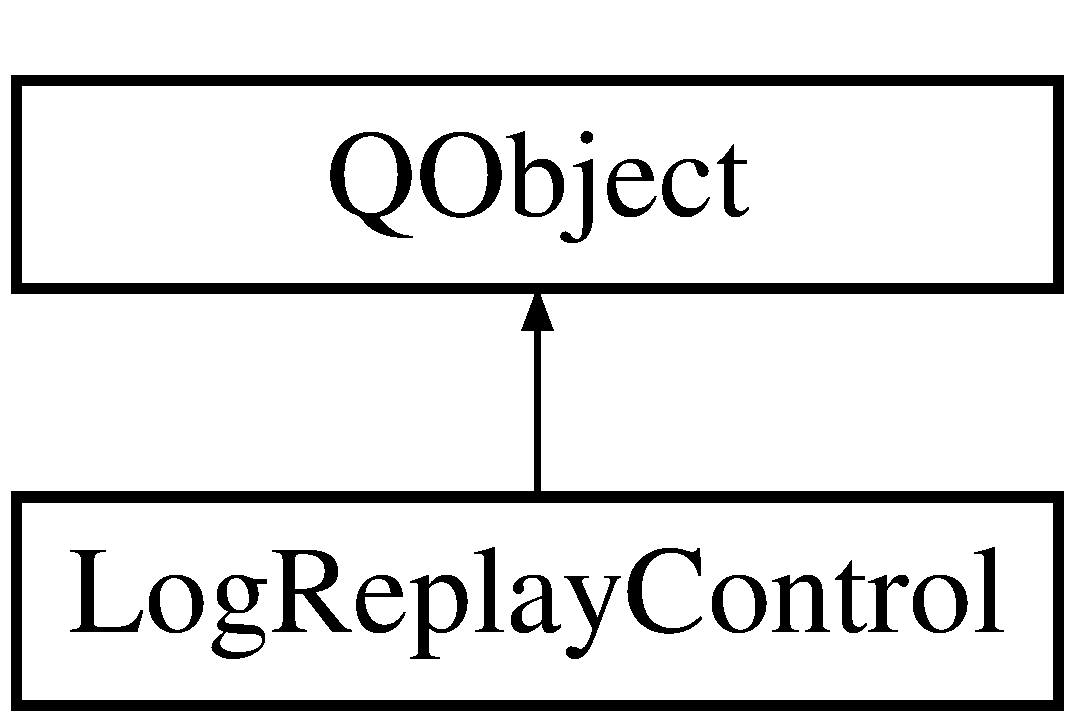
\includegraphics[height=2.000000cm]{de/d5e/a00007}
\end{center}
\end{figure}
\subsection*{Public Slots}
\subsection*{Signals}
\subsection*{Static Public Member Functions}
\subsection*{Private Member Functions}
\subsection*{Private Attributes}
\subsection*{Static Private Attributes}


\subsection{Detailed Description}


\subsection{Constructor \& Destructor Documentation}
\hypertarget{a00007_ab0b79423b2b67162e12b82b5458610c6}{\index{Log\-Replay\-Control@{Log\-Replay\-Control}!Log\-Replay\-Control@{Log\-Replay\-Control}}
\index{Log\-Replay\-Control@{Log\-Replay\-Control}!LogReplayControl@{Log\-Replay\-Control}}
\subsubsection[{Log\-Replay\-Control}]{\setlength{\rightskip}{0pt plus 5cm}{\bf Log\-Replay\-Control} (
\begin{DoxyParamCaption}
{}
\end{DoxyParamCaption}
)\hspace{0.3cm}{\ttfamily [private]}}}\label{a00007_ab0b79423b2b67162e12b82b5458610c6}


Constructor. 


\begin{DoxyParams}{Parameters}
{\em none} & \\
\hline
\end{DoxyParams}

\begin{DoxyExceptions}{Exceptions}
{\em none} & \\
\hline
\end{DoxyExceptions}
\begin{DoxyReturn}{Returns}
\hyperlink{a00007}{Log\-Replay\-Control} instance 
\end{DoxyReturn}

\begin{DoxyCode}
6 \{
7     \textcolor{comment}{/*m\_pStartPause = new ToggleButton();}
8 \textcolor{comment}{    m\_pIncSpeed = new QPushButton();}
9 \textcolor{comment}{    m\_pDecSpeed = new QPushButton();}
10 \textcolor{comment}{    m\_pStop = new QPushButton();*/}
11     \hyperlink{a00007_ae4449bc255d96573e420df2efe33e83e}{m\_iData} = 0;
12     \hyperlink{a00007_a9b60d9b0fc5bc08efbad926439d7933c}{m\_bReverse} = \textcolor{keyword}{false};
13     connect(&\hyperlink{a00007_a751177401fcce70c122d30de758b05a0}{m\_pReplayTimer}, SIGNAL(timeout()), \textcolor{keyword}{this}, SLOT(\hyperlink{a00007_aa4dbf9e6f1a5549a0444ad2995e8748b}{replay}()));
14 \}
\end{DoxyCode}
\hypertarget{a00007_a9a1182668244140773a52ee54723c8fd}{\index{Log\-Replay\-Control@{Log\-Replay\-Control}!$\sim$\-Log\-Replay\-Control@{$\sim$\-Log\-Replay\-Control}}
\index{$\sim$\-Log\-Replay\-Control@{$\sim$\-Log\-Replay\-Control}!LogReplayControl@{Log\-Replay\-Control}}
\subsubsection[{$\sim$\-Log\-Replay\-Control}]{\setlength{\rightskip}{0pt plus 5cm}$\sim${\bf Log\-Replay\-Control} (
\begin{DoxyParamCaption}
{}
\end{DoxyParamCaption}
)\hspace{0.3cm}{\ttfamily [private]}}}\label{a00007_a9a1182668244140773a52ee54723c8fd}


Destructor. 


\begin{DoxyParams}{Parameters}
{\em none} & \\
\hline
\end{DoxyParams}

\begin{DoxyExceptions}{Exceptions}
{\em none} & \\
\hline
\end{DoxyExceptions}
\begin{DoxyReturn}{Returns}
none 
\end{DoxyReturn}

\begin{DoxyCode}
26 \{
27 \}
\end{DoxyCode}


\subsection{Member Function Documentation}
\hypertarget{a00007_a9b83f0fc7f06bee951213dd4b22e0e93}{\index{Log\-Replay\-Control@{Log\-Replay\-Control}!backward@{backward}}
\index{backward@{backward}!LogReplayControl@{Log\-Replay\-Control}}
\subsubsection[{backward}]{\setlength{\rightskip}{0pt plus 5cm}void backward (
\begin{DoxyParamCaption}
{}
\end{DoxyParamCaption}
)\hspace{0.3cm}{\ttfamily [slot]}}}\label{a00007_a9b83f0fc7f06bee951213dd4b22e0e93}

\begin{DoxyCode}
77 \{
78     \textcolor{keywordflow}{if} (\hyperlink{a00007_a9b60d9b0fc5bc08efbad926439d7933c}{m\_bReverse} == \textcolor{keyword}{true})
79     \{
80         \hyperlink{a00007_a751177401fcce70c122d30de758b05a0}{m\_pReplayTimer}.setInterval(\hyperlink{a00007_a751177401fcce70c122d30de758b05a0}{m\_pReplayTimer}.interval() + 50);
81     \}
82     \textcolor{keywordflow}{else}
83     \{
84         \hyperlink{a00007_a751177401fcce70c122d30de758b05a0}{m\_pReplayTimer}.setInterval(\hyperlink{a00007_a751177401fcce70c122d30de758b05a0}{m\_pReplayTimer}.interval() - 50);
85 
86         \textcolor{keywordflow}{if} (\hyperlink{a00007_a751177401fcce70c122d30de758b05a0}{m\_pReplayTimer}.interval() <= 0)
87         \{
88             \hyperlink{a00007_a751177401fcce70c122d30de758b05a0}{m\_pReplayTimer}.setInterval(50);
89             \hyperlink{a00007_a9b60d9b0fc5bc08efbad926439d7933c}{m\_bReverse} = \textcolor{keyword}{true};
90         \}
91     \}
92 \}
\end{DoxyCode}
\hypertarget{a00007_a7de2a543986e45b9083c69f6138bf079}{\index{Log\-Replay\-Control@{Log\-Replay\-Control}!forward@{forward}}
\index{forward@{forward}!LogReplayControl@{Log\-Replay\-Control}}
\subsubsection[{forward}]{\setlength{\rightskip}{0pt plus 5cm}void forward (
\begin{DoxyParamCaption}
{}
\end{DoxyParamCaption}
)\hspace{0.3cm}{\ttfamily [slot]}}}\label{a00007_a7de2a543986e45b9083c69f6138bf079}

\begin{DoxyCode}
59 \{
60     \textcolor{keywordflow}{if} (\hyperlink{a00007_a9b60d9b0fc5bc08efbad926439d7933c}{m\_bReverse} == \textcolor{keyword}{false})
61     \{
62         \hyperlink{a00007_a751177401fcce70c122d30de758b05a0}{m\_pReplayTimer}.setInterval(\hyperlink{a00007_a751177401fcce70c122d30de758b05a0}{m\_pReplayTimer}.interval() + 50);
63     \}
64     \textcolor{keywordflow}{else}
65     \{
66         \hyperlink{a00007_a751177401fcce70c122d30de758b05a0}{m\_pReplayTimer}.setInterval(\hyperlink{a00007_a751177401fcce70c122d30de758b05a0}{m\_pReplayTimer}.interval() - 50);
67 
68         \textcolor{keywordflow}{if} (\hyperlink{a00007_a751177401fcce70c122d30de758b05a0}{m\_pReplayTimer}.interval() <= 0)
69         \{
70             \hyperlink{a00007_a751177401fcce70c122d30de758b05a0}{m\_pReplayTimer}.setInterval(50);
71             \hyperlink{a00007_a9b60d9b0fc5bc08efbad926439d7933c}{m\_bReverse} = \textcolor{keyword}{false};
72         \}
73     \}
74 \}
\end{DoxyCode}
\hypertarget{a00007_ac64f2ec114d4ab8dd8ed8dd31f243454}{\index{Log\-Replay\-Control@{Log\-Replay\-Control}!geolocation@{geolocation}}
\index{geolocation@{geolocation}!LogReplayControl@{Log\-Replay\-Control}}
\subsubsection[{geolocation}]{\setlength{\rightskip}{0pt plus 5cm}void geolocation (
\begin{DoxyParamCaption}
\item[{double}]{latitude, }
\item[{double}]{longitude, }
\item[{double}]{altitude, }
\item[{double}]{heading}
\end{DoxyParamCaption}
)\hspace{0.3cm}{\ttfamily [signal]}}}\label{a00007_ac64f2ec114d4ab8dd8ed8dd31f243454}


Update M\-U\-A\-V geolocation. 


\begin{DoxyParams}{Parameters}
{\em x} & longitude double \\
\hline
{\em y} & latitude double \\
\hline
{\em z} & altitude double \\
\hline
{\em yaw} & heading double \\
\hline
\end{DoxyParams}

\begin{DoxyExceptions}{Exceptions}
{\em none} & \\
\hline
\end{DoxyExceptions}
\begin{DoxyReturn}{Returns}
none 
\end{DoxyReturn}
\hypertarget{a00007_adb2b1b18fad4caaafde371f991525f38}{\index{Log\-Replay\-Control@{Log\-Replay\-Control}!get\-Instance@{get\-Instance}}
\index{get\-Instance@{get\-Instance}!LogReplayControl@{Log\-Replay\-Control}}
\subsubsection[{get\-Instance}]{\setlength{\rightskip}{0pt plus 5cm}{\bf Log\-Replay\-Control} $\ast$ get\-Instance (
\begin{DoxyParamCaption}
{}
\end{DoxyParamCaption}
)\hspace{0.3cm}{\ttfamily [static]}}}\label{a00007_adb2b1b18fad4caaafde371f991525f38}


\hyperlink{a00007}{Log\-Replay\-Control} lone instance getter. 


\begin{DoxyParams}{Parameters}
{\em none} & \\
\hline
\end{DoxyParams}

\begin{DoxyExceptions}{Exceptions}
{\em none} & \\
\hline
\end{DoxyExceptions}
\begin{DoxyReturn}{Returns}
lone instance Mission\-Control$\ast$ 
\end{DoxyReturn}

\begin{DoxyCode}
30 \{
31     \textcolor{keywordflow}{if} (\hyperlink{a00007_a72df5eacd5c7ea6c052e02000643fd7e}{singleton} == NULL)
32     \{
33         \hyperlink{a00007_a72df5eacd5c7ea6c052e02000643fd7e}{singleton} = \textcolor{keyword}{new} \hyperlink{a00007_ab0b79423b2b67162e12b82b5458610c6}{LogReplayControl}();
34     \}
35 
36     \textcolor{keywordflow}{return} \hyperlink{a00007_a72df5eacd5c7ea6c052e02000643fd7e}{singleton};
37 \}
\end{DoxyCode}
\hypertarget{a00007_aae9d52caad9fb2892deeb25596cfd2ab}{\index{Log\-Replay\-Control@{Log\-Replay\-Control}!kill@{kill}}
\index{kill@{kill}!LogReplayControl@{Log\-Replay\-Control}}
\subsubsection[{kill}]{\setlength{\rightskip}{0pt plus 5cm}void kill (
\begin{DoxyParamCaption}
{}
\end{DoxyParamCaption}
)\hspace{0.3cm}{\ttfamily [static]}}}\label{a00007_aae9d52caad9fb2892deeb25596cfd2ab}


Instance killer. 


\begin{DoxyParams}{Parameters}
{\em none} & \\
\hline
\end{DoxyParams}

\begin{DoxyExceptions}{Exceptions}
{\em none} & \\
\hline
\end{DoxyExceptions}
\begin{DoxyReturn}{Returns}
none 
\end{DoxyReturn}

\begin{DoxyCode}
17 \{
18     \textcolor{keywordflow}{if} (\hyperlink{a00007_a72df5eacd5c7ea6c052e02000643fd7e}{singleton} != NULL)
19     \{
20         \textcolor{keyword}{delete} \hyperlink{a00007_a72df5eacd5c7ea6c052e02000643fd7e}{singleton};
21         \hyperlink{a00007_a72df5eacd5c7ea6c052e02000643fd7e}{singleton} = NULL;
22     \}
23 \}
\end{DoxyCode}
\hypertarget{a00007_a2d8621c7c4f4531bee805e91595b6b76}{\index{Log\-Replay\-Control@{Log\-Replay\-Control}!open\-Log@{open\-Log}}
\index{open\-Log@{open\-Log}!LogReplayControl@{Log\-Replay\-Control}}
\subsubsection[{open\-Log}]{\setlength{\rightskip}{0pt plus 5cm}void open\-Log (
\begin{DoxyParamCaption}
{}
\end{DoxyParamCaption}
)\hspace{0.3cm}{\ttfamily [slot]}}}\label{a00007_a2d8621c7c4f4531bee805e91595b6b76}

\begin{DoxyCode}
135 \{
136         \textcolor{comment}{//QString name = QFileDialog::getOpenFileName(NULL, ResourceControl::getText("selectLogTitle"),}
137         \textcolor{comment}{//  "", "Data log files (*.csv)");}
138     QString name = \textcolor{stringliteral}{"Hola"};
139 
140     \textcolor{keywordflow}{if} (name != \textcolor{stringliteral}{""})
141     \{
142         QString line;
143         QStringList lineSplit;
144 
145         QFile file(name);
146 
147         \textcolor{keywordflow}{if} (file.open(QIODevice::ReadOnly))
148         \{
149             QTextStream textStream(&file);
150             line = textStream.readLine();
151 
152             \textcolor{keywordflow}{while} (!textStream.atEnd())
153             \{
154                 line = textStream.readLine();
155                 lineSplit = line.split(\textcolor{stringliteral}{";"});
156 
157                 \hyperlink{a00007_a684fa381f2a0f0098edcbc7c7b3ea93d}{m\_aLatitude}.push\_back(lineSplit.at(1).toDouble());
158                 \hyperlink{a00007_aa900c1e4f1eea660e8f52de1e2109bad}{m\_aLongitude}.push\_back(lineSplit.at(2).toDouble());
159                 \hyperlink{a00007_a9d1929fdd4a8b1a587c97688bc91037b}{m\_aAltitude}.push\_back(lineSplit.at(3).toDouble());
160                 \hyperlink{a00007_a9eed7e988005e7291b4e9d401c678693}{m\_aHeading}.push\_back(lineSplit.at(4).toDouble());
161             \}
162         \}
163     \}
164 \}
\end{DoxyCode}
\hypertarget{a00007_a7167f5c196fc5e167bfabde1a730e81d}{\index{Log\-Replay\-Control@{Log\-Replay\-Control}!pause@{pause}}
\index{pause@{pause}!LogReplayControl@{Log\-Replay\-Control}}
\subsubsection[{pause}]{\setlength{\rightskip}{0pt plus 5cm}void pause (
\begin{DoxyParamCaption}
{}
\end{DoxyParamCaption}
)\hspace{0.3cm}{\ttfamily [slot]}}}\label{a00007_a7167f5c196fc5e167bfabde1a730e81d}

\begin{DoxyCode}
46 \{
47     \hyperlink{a00007_a751177401fcce70c122d30de758b05a0}{m\_pReplayTimer}.stop();
48 \}
\end{DoxyCode}
\hypertarget{a00007_aa4dbf9e6f1a5549a0444ad2995e8748b}{\index{Log\-Replay\-Control@{Log\-Replay\-Control}!replay@{replay}}
\index{replay@{replay}!LogReplayControl@{Log\-Replay\-Control}}
\subsubsection[{replay}]{\setlength{\rightskip}{0pt plus 5cm}void replay (
\begin{DoxyParamCaption}
{}
\end{DoxyParamCaption}
)\hspace{0.3cm}{\ttfamily [slot]}}}\label{a00007_aa4dbf9e6f1a5549a0444ad2995e8748b}

\begin{DoxyCode}
95 \{
96     \textcolor{keywordflow}{if} (\hyperlink{a00007_a9b60d9b0fc5bc08efbad926439d7933c}{m\_bReverse} == \textcolor{keyword}{false})
97     \{
98         \textcolor{keywordflow}{if} (\hyperlink{a00007_ae4449bc255d96573e420df2efe33e83e}{m\_iData} > \hyperlink{a00007_a684fa381f2a0f0098edcbc7c7b3ea93d}{m\_aLatitude}.length())
99         \{
100             \hyperlink{a00007_a8c528baf37154d347366083f0f816846}{stop}();
101         \}
102         \textcolor{keywordflow}{else} \textcolor{keywordflow}{if} (\hyperlink{a00007_ae4449bc255d96573e420df2efe33e83e}{m\_iData} < \hyperlink{a00007_a684fa381f2a0f0098edcbc7c7b3ea93d}{m\_aLatitude}.length())
103         \{
104             emit \hyperlink{a00007_ac64f2ec114d4ab8dd8ed8dd31f243454}{geolocation}(\hyperlink{a00007_a684fa381f2a0f0098edcbc7c7b3ea93d}{m\_aLatitude}[\hyperlink{a00007_ae4449bc255d96573e420df2efe33e83e}{m\_iData}], 
      \hyperlink{a00007_aa900c1e4f1eea660e8f52de1e2109bad}{m\_aLongitude}[m\_iData], \hyperlink{a00007_a9d1929fdd4a8b1a587c97688bc91037b}{m\_aAltitude}[m\_iData], 0);
105             emit \hyperlink{a00007_aa3c54f0958638486df2b69a9b53c5d7f}{updateHeading}(\hyperlink{a00007_a9eed7e988005e7291b4e9d401c678693}{m\_aHeading}[\hyperlink{a00007_ae4449bc255d96573e420df2efe33e83e}{m\_iData}]);
106 
107             \hyperlink{a00007_ae4449bc255d96573e420df2efe33e83e}{m\_iData}++;
108         \}
109         \textcolor{keywordflow}{else}
110         \{
111             \hyperlink{a00007_a8c528baf37154d347366083f0f816846}{stop}();
112         \}
113     \}
114     \textcolor{keywordflow}{else}
115     \{
116         \textcolor{keywordflow}{if} (\hyperlink{a00007_ae4449bc255d96573e420df2efe33e83e}{m\_iData} < 0)
117         \{
118             \hyperlink{a00007_a8c528baf37154d347366083f0f816846}{stop}();
119         \}
120         \textcolor{keywordflow}{else} \textcolor{keywordflow}{if} (\hyperlink{a00007_ae4449bc255d96573e420df2efe33e83e}{m\_iData} < \hyperlink{a00007_a684fa381f2a0f0098edcbc7c7b3ea93d}{m\_aLatitude}.length())
121         \{
122             emit \hyperlink{a00007_ac64f2ec114d4ab8dd8ed8dd31f243454}{geolocation}(\hyperlink{a00007_a684fa381f2a0f0098edcbc7c7b3ea93d}{m\_aLatitude}[\hyperlink{a00007_ae4449bc255d96573e420df2efe33e83e}{m\_iData}], 
      \hyperlink{a00007_aa900c1e4f1eea660e8f52de1e2109bad}{m\_aLongitude}[m\_iData], \hyperlink{a00007_a9d1929fdd4a8b1a587c97688bc91037b}{m\_aAltitude}[m\_iData], 0);
123             emit \hyperlink{a00007_aa3c54f0958638486df2b69a9b53c5d7f}{updateHeading}(\hyperlink{a00007_a9eed7e988005e7291b4e9d401c678693}{m\_aHeading}[\hyperlink{a00007_ae4449bc255d96573e420df2efe33e83e}{m\_iData}]);
124 
125             \hyperlink{a00007_ae4449bc255d96573e420df2efe33e83e}{m\_iData}--;
126         \}
127         \textcolor{keywordflow}{else}
128         \{
129             \hyperlink{a00007_a8c528baf37154d347366083f0f816846}{stop}();
130         \}
131     \}
132 \}
\end{DoxyCode}
\hypertarget{a00007_a60de64d75454385b23995437f1d72669}{\index{Log\-Replay\-Control@{Log\-Replay\-Control}!start@{start}}
\index{start@{start}!LogReplayControl@{Log\-Replay\-Control}}
\subsubsection[{start}]{\setlength{\rightskip}{0pt plus 5cm}void start (
\begin{DoxyParamCaption}
{}
\end{DoxyParamCaption}
)\hspace{0.3cm}{\ttfamily [slot]}}}\label{a00007_a60de64d75454385b23995437f1d72669}

\begin{DoxyCode}
40 \{
41     \hyperlink{a00007_a751177401fcce70c122d30de758b05a0}{m\_pReplayTimer}.start(200);
42     \hyperlink{a00001_afebd43c1f2afd7ec0eb35f99e50f0964}{CommunicationControl::getInstance}()->\hyperlink{a00001_a8c528baf37154d347366083f0f816846}{stop}();
43 \}
\end{DoxyCode}
\hypertarget{a00007_a8c528baf37154d347366083f0f816846}{\index{Log\-Replay\-Control@{Log\-Replay\-Control}!stop@{stop}}
\index{stop@{stop}!LogReplayControl@{Log\-Replay\-Control}}
\subsubsection[{stop}]{\setlength{\rightskip}{0pt plus 5cm}void stop (
\begin{DoxyParamCaption}
{}
\end{DoxyParamCaption}
)\hspace{0.3cm}{\ttfamily [slot]}}}\label{a00007_a8c528baf37154d347366083f0f816846}

\begin{DoxyCode}
51 \{
52     \hyperlink{a00007_a751177401fcce70c122d30de758b05a0}{m\_pReplayTimer}.stop();
53 
54     \hyperlink{a00007_ae4449bc255d96573e420df2efe33e83e}{m\_iData} = 0;
55     \hyperlink{a00007_a9b60d9b0fc5bc08efbad926439d7933c}{m\_bReverse} = \textcolor{keyword}{false};
56 \}
\end{DoxyCode}
\hypertarget{a00007_aa3c54f0958638486df2b69a9b53c5d7f}{\index{Log\-Replay\-Control@{Log\-Replay\-Control}!update\-Heading@{update\-Heading}}
\index{update\-Heading@{update\-Heading}!LogReplayControl@{Log\-Replay\-Control}}
\subsubsection[{update\-Heading}]{\setlength{\rightskip}{0pt plus 5cm}void update\-Heading (
\begin{DoxyParamCaption}
\item[{double}]{p\-\_\-p\-Value}
\end{DoxyParamCaption}
)\hspace{0.3cm}{\ttfamily [signal]}}}\label{a00007_aa3c54f0958638486df2b69a9b53c5d7f}


Update heading value. 


\begin{DoxyParams}{Parameters}
{\em p\-\_\-p\-Value} & heading value double \\
\hline
\end{DoxyParams}

\begin{DoxyExceptions}{Exceptions}
{\em none} & \\
\hline
\end{DoxyExceptions}
\begin{DoxyReturn}{Returns}
none 
\end{DoxyReturn}


\subsection{Field Documentation}
\hypertarget{a00007_a9d1929fdd4a8b1a587c97688bc91037b}{\index{Log\-Replay\-Control@{Log\-Replay\-Control}!m\-\_\-a\-Altitude@{m\-\_\-a\-Altitude}}
\index{m\-\_\-a\-Altitude@{m\-\_\-a\-Altitude}!LogReplayControl@{Log\-Replay\-Control}}
\subsubsection[{m\-\_\-a\-Altitude}]{\setlength{\rightskip}{0pt plus 5cm}Q\-List$<$double$>$ m\-\_\-a\-Altitude\hspace{0.3cm}{\ttfamily [private]}}}\label{a00007_a9d1929fdd4a8b1a587c97688bc91037b}
\hypertarget{a00007_a9eed7e988005e7291b4e9d401c678693}{\index{Log\-Replay\-Control@{Log\-Replay\-Control}!m\-\_\-a\-Heading@{m\-\_\-a\-Heading}}
\index{m\-\_\-a\-Heading@{m\-\_\-a\-Heading}!LogReplayControl@{Log\-Replay\-Control}}
\subsubsection[{m\-\_\-a\-Heading}]{\setlength{\rightskip}{0pt plus 5cm}Q\-List$<$double$>$ m\-\_\-a\-Heading\hspace{0.3cm}{\ttfamily [private]}}}\label{a00007_a9eed7e988005e7291b4e9d401c678693}
\hypertarget{a00007_a684fa381f2a0f0098edcbc7c7b3ea93d}{\index{Log\-Replay\-Control@{Log\-Replay\-Control}!m\-\_\-a\-Latitude@{m\-\_\-a\-Latitude}}
\index{m\-\_\-a\-Latitude@{m\-\_\-a\-Latitude}!LogReplayControl@{Log\-Replay\-Control}}
\subsubsection[{m\-\_\-a\-Latitude}]{\setlength{\rightskip}{0pt plus 5cm}Q\-List$<$double$>$ m\-\_\-a\-Latitude\hspace{0.3cm}{\ttfamily [private]}}}\label{a00007_a684fa381f2a0f0098edcbc7c7b3ea93d}
\hypertarget{a00007_aa900c1e4f1eea660e8f52de1e2109bad}{\index{Log\-Replay\-Control@{Log\-Replay\-Control}!m\-\_\-a\-Longitude@{m\-\_\-a\-Longitude}}
\index{m\-\_\-a\-Longitude@{m\-\_\-a\-Longitude}!LogReplayControl@{Log\-Replay\-Control}}
\subsubsection[{m\-\_\-a\-Longitude}]{\setlength{\rightskip}{0pt plus 5cm}Q\-List$<$double$>$ m\-\_\-a\-Longitude\hspace{0.3cm}{\ttfamily [private]}}}\label{a00007_aa900c1e4f1eea660e8f52de1e2109bad}
\hypertarget{a00007_a9b60d9b0fc5bc08efbad926439d7933c}{\index{Log\-Replay\-Control@{Log\-Replay\-Control}!m\-\_\-b\-Reverse@{m\-\_\-b\-Reverse}}
\index{m\-\_\-b\-Reverse@{m\-\_\-b\-Reverse}!LogReplayControl@{Log\-Replay\-Control}}
\subsubsection[{m\-\_\-b\-Reverse}]{\setlength{\rightskip}{0pt plus 5cm}bool m\-\_\-b\-Reverse\hspace{0.3cm}{\ttfamily [private]}}}\label{a00007_a9b60d9b0fc5bc08efbad926439d7933c}
\hypertarget{a00007_ae4449bc255d96573e420df2efe33e83e}{\index{Log\-Replay\-Control@{Log\-Replay\-Control}!m\-\_\-i\-Data@{m\-\_\-i\-Data}}
\index{m\-\_\-i\-Data@{m\-\_\-i\-Data}!LogReplayControl@{Log\-Replay\-Control}}
\subsubsection[{m\-\_\-i\-Data}]{\setlength{\rightskip}{0pt plus 5cm}int m\-\_\-i\-Data\hspace{0.3cm}{\ttfamily [private]}}}\label{a00007_ae4449bc255d96573e420df2efe33e83e}
\hypertarget{a00007_a751177401fcce70c122d30de758b05a0}{\index{Log\-Replay\-Control@{Log\-Replay\-Control}!m\-\_\-p\-Replay\-Timer@{m\-\_\-p\-Replay\-Timer}}
\index{m\-\_\-p\-Replay\-Timer@{m\-\_\-p\-Replay\-Timer}!LogReplayControl@{Log\-Replay\-Control}}
\subsubsection[{m\-\_\-p\-Replay\-Timer}]{\setlength{\rightskip}{0pt plus 5cm}Q\-Timer m\-\_\-p\-Replay\-Timer\hspace{0.3cm}{\ttfamily [private]}}}\label{a00007_a751177401fcce70c122d30de758b05a0}
\hypertarget{a00007_a72df5eacd5c7ea6c052e02000643fd7e}{\index{Log\-Replay\-Control@{Log\-Replay\-Control}!singleton@{singleton}}
\index{singleton@{singleton}!LogReplayControl@{Log\-Replay\-Control}}
\subsubsection[{singleton}]{\setlength{\rightskip}{0pt plus 5cm}{\bf Log\-Replay\-Control} $\ast$ singleton = N\-U\-L\-L\hspace{0.3cm}{\ttfamily [static]}, {\ttfamily [private]}}}\label{a00007_a72df5eacd5c7ea6c052e02000643fd7e}


The documentation for this class was generated from the following files\-:\begin{DoxyCompactItemize}
\item 
\hyperlink{a00026}{Log\-Replay\-Control.\-h}\item 
\hyperlink{a00025}{Log\-Replay\-Control.\-cpp}\end{DoxyCompactItemize}

\hypertarget{a00008}{\section{M\-A\-R\-C\-S Class Reference}
\label{a00008}\index{M\-A\-R\-C\-S@{M\-A\-R\-C\-S}}
}


{\ttfamily \#include \char`\"{}marcs.\-h\char`\"{}}

Inheritance diagram for M\-A\-R\-C\-S\-:\begin{figure}[H]
\begin{center}
\leavevmode
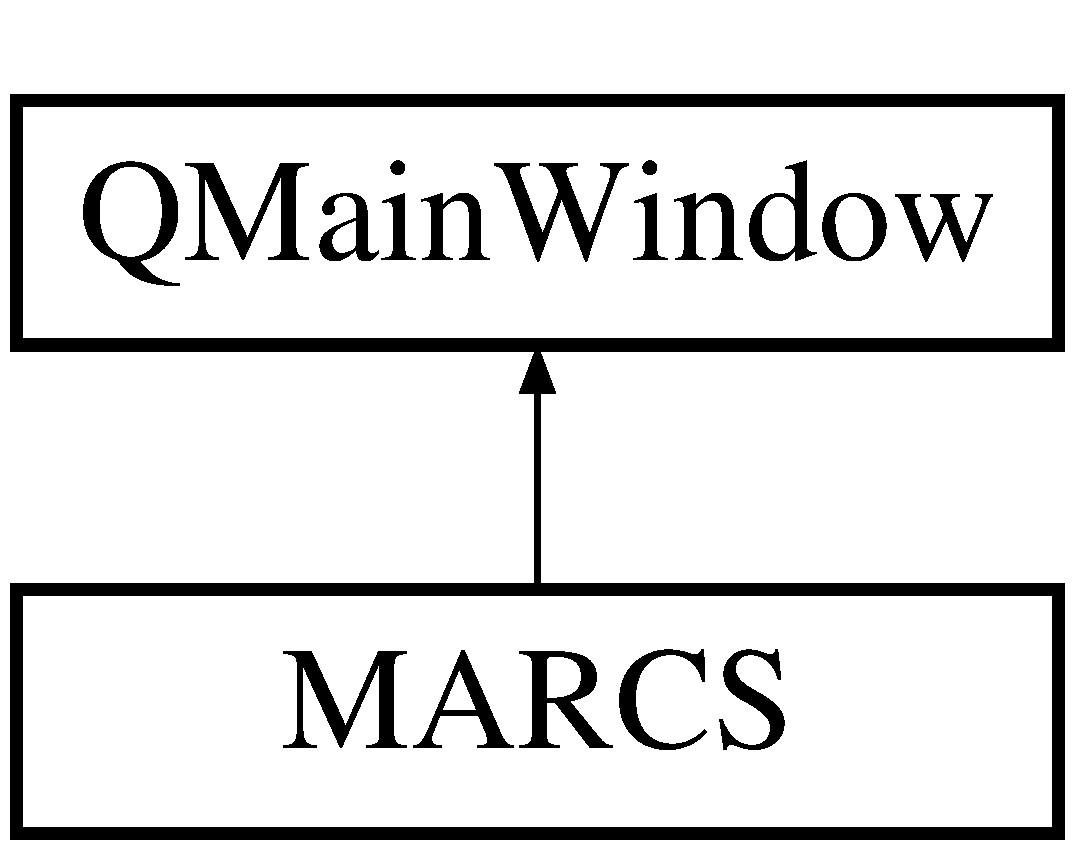
\includegraphics[height=2.000000cm]{d4/dee/a00008}
\end{center}
\end{figure}
\subsection*{Public Slots}
\subsection*{Signals}
\subsection*{Public Member Functions}
\subsection*{Private Slots}
\subsection*{Private Attributes}


\subsection{Detailed Description}


\subsection{Constructor \& Destructor Documentation}
\hypertarget{a00008_ae5f86b696629408c70e44a87d08ec5ac}{\index{M\-A\-R\-C\-S@{M\-A\-R\-C\-S}!M\-A\-R\-C\-S@{M\-A\-R\-C\-S}}
\index{M\-A\-R\-C\-S@{M\-A\-R\-C\-S}!MARCS@{M\-A\-R\-C\-S}}
\subsubsection[{M\-A\-R\-C\-S}]{\setlength{\rightskip}{0pt plus 5cm}{\bf M\-A\-R\-C\-S} (
\begin{DoxyParamCaption}
\item[{Q\-Widget $\ast$}]{parent = {\ttfamily 0}}
\end{DoxyParamCaption}
)\hspace{0.3cm}{\ttfamily [explicit]}}}\label{a00008_ae5f86b696629408c70e44a87d08ec5ac}

\begin{DoxyCode}
6                             :
7     QMainWindow(parent),
8     \hyperlink{a00008_a6dc041ef6a2ffb329928d2913e8344e6}{ui}(\textcolor{keyword}{new} Ui::MARCS)
9 \{
10 
11     \hyperlink{a00008_a6dc041ef6a2ffb329928d2913e8344e6}{ui}->setupUi(\textcolor{keyword}{this});
12 
13     \hyperlink{a00008_afa3cdab37d8290f081abb0c5fb137230}{iconOn}.addFile(QString::fromUtf8(\textcolor{stringliteral}{":/new/prefix1/icon/engineOn.png"}), QSize(), QIcon::Normal, 
      QIcon::Off);
14     \hyperlink{a00008_a8b9cd945dedf4c271116b676b3ca723f}{iconOff}.addFile(QString::fromUtf8(\textcolor{stringliteral}{":/new/prefix1/icon/engineOff.png"}), QSize(), QIcon::Normal, 
      QIcon::Off);
15     \hyperlink{a00008_a0bf2452bb61d9523e3c8e53a28969dca}{iconTakeOff}.addFile(QString::fromUtf8(\textcolor{stringliteral}{":/new/prefix1/icon/takeoff.png"}), QSize(), 
      QIcon::Normal, QIcon::Off);
16     \hyperlink{a00008_a2f2a3f2df70bdcdde196ec849469359c}{iconLand}.addFile(QString::fromUtf8(\textcolor{stringliteral}{":/new/prefix1/icon/land.png"}), QSize(), QIcon::Normal, 
      QIcon::Off);
17 
18     \hyperlink{a00008_ab78e87803316b7303d0f8697c7c0f253}{place} =  \textcolor{keyword}{new} GeoDataPlacemark( \textcolor{stringliteral}{""} );
19     \hyperlink{a00008_a8b0f68f97ddd8c30ad31efa6919778ee}{document} = \textcolor{keyword}{new} GeoDataDocument();
20     \hyperlink{a00008_a5023376f47e503f88c7ee3bb2c096bb1}{placemarkRPA} = \textcolor{keyword}{new} GeoDataPlacemark( \textcolor{stringliteral}{""} );
21     \hyperlink{a00008_a5204b956a1ced61beed9e7db0e8289df}{placemarkHome} = \textcolor{keyword}{new} GeoDataPlacemark( \textcolor{stringliteral}{""} );
22     \hyperlink{a00008_a0e901909eecb8e5845b160761528be11}{placemarkMark} = \textcolor{keyword}{new} GeoDataPlacemark( \textcolor{stringliteral}{""} );
23     \hyperlink{a00008_a3ccaefd3393a3447a3a10d94ab67b0f9}{styleArchRPA} = \textcolor{keyword}{new} GeoDataStyle();
24     \hyperlink{a00008_a06e86babaf03affa3f647a3650df417e}{styleArchHome} = \textcolor{keyword}{new} GeoDataStyle();
25     \hyperlink{a00008_ab3cb2d82e21852d6e82932d21a1b3f41}{styleArchMark} = \textcolor{keyword}{new} GeoDataStyle();
26 
27     \hyperlink{a00008_ab48a9573e6326f95a2bd888734fa7827}{documentRPA} = \textcolor{keyword}{new} GeoDataDocument();
28     \hyperlink{a00008_a5485f3186e5ee43d5cb40af7a555bb7e}{documentHome} = \textcolor{keyword}{new} GeoDataDocument();
29     \hyperlink{a00008_a9480c34bf64d45bdea5c4d162eb2bfd4}{documentMark} = \textcolor{keyword}{new} GeoDataDocument();
30     \hyperlink{a00008_a92b8cb43df3f03b62d33cd4e04550941}{myCom} = \textcolor{keyword}{new} \hyperlink{a00002}{ComThread}();
31     \hyperlink{a00008_aad93f0b04d6ea6ac097124ef453bef9d}{numWpText} = \textcolor{keyword}{new} \textcolor{keywordtype}{char}[32];
32 
33     \hyperlink{a00008_af75d5c0cb380ae793706dd041af8469a}{ItemLon} = \textcolor{keyword}{new} QTableWidgetItem;
34     \hyperlink{a00008_a4d1885cf51ba7e0ad51da1563a8e956e}{ItemLat} = \textcolor{keyword}{new} QTableWidgetItem;
35     \hyperlink{a00008_a115144783225aa4ada70742197268579}{ItemAlt} = \textcolor{keyword}{new} QTableWidgetItem;
36     \hyperlink{a00008_a19ad1cbb017398e3607b99248ad0098e}{ItemHdg} = \textcolor{keyword}{new} QTableWidgetItem;
37     \hyperlink{a00008_acf2c8407d4d41ac02f8a408056b0b4b9}{ItemName} = \textcolor{keyword}{new} QTableWidgetItem;
38 
39     \hyperlink{a00008_a0dfc989df25831d61f32925ac130d65d}{ItemMarkAlt} = \textcolor{keyword}{new} QTableWidgetItem;
40     \hyperlink{a00008_aba4af01dc350023f13a5b2733213bcbf}{ItemMarkHdg} = \textcolor{keyword}{new} QTableWidgetItem;
41     \hyperlink{a00008_a180185f28d7e25ea00f4ba8ceab18683}{ItemMarkLat} = \textcolor{keyword}{new} QTableWidgetItem;
42     \hyperlink{a00008_a5d50927e21149ddeb88d4a8673c66bcd}{ItemMarkLon} = \textcolor{keyword}{new} QTableWidgetItem;
43     \hyperlink{a00008_a64a4c8982cd17f0be916f6b5f5f6054f}{ItemMarkNum} = \textcolor{keyword}{new} QTableWidgetItem;
44 
45     \hyperlink{a00008_a8ea0fa63ef52288523cbe2d67e5ace69}{m\_pComWindow} = \textcolor{keyword}{new} QMainWindow();
46     \hyperlink{a00008_a3dcd7d9704d0284fd91442e4cc1ec721}{layout} = \textcolor{keyword}{new} QGridLayout();
47     \hyperlink{a00008_a549c5bee62879e34e9d21701730a2907}{widget} = \textcolor{keyword}{new} QWidget();
48     \hyperlink{a00008_a701fe8b63e4569ef364331319c38d6dd}{m\_pComList} = \textcolor{keyword}{new} QComboBox();
49     \hyperlink{a00008_a6cc0e75acee9ad59ae06de6371fa3c14}{m\_pValidCom} = \textcolor{keyword}{new} QPushButton(\textcolor{stringliteral}{"Valid"});
50     \hyperlink{a00008_ab216d58a00329023c2ded930bc085ff1}{m\_pLabel} = \textcolor{keyword}{new} QLabel(\textcolor{stringliteral}{"Serial port"}) ;
51 
52     \hyperlink{a00008_a3dcd7d9704d0284fd91442e4cc1ec721}{layout}->addWidget(\hyperlink{a00008_ab216d58a00329023c2ded930bc085ff1}{m\_pLabel} , 0, 0);
53     \hyperlink{a00008_a3dcd7d9704d0284fd91442e4cc1ec721}{layout}->addWidget(\hyperlink{a00008_a701fe8b63e4569ef364331319c38d6dd}{m\_pComList}, 0, 1);
54     \hyperlink{a00008_a3dcd7d9704d0284fd91442e4cc1ec721}{layout}->addWidget(\hyperlink{a00008_a6cc0e75acee9ad59ae06de6371fa3c14}{m\_pValidCom}, 1, 0, 1, 2);
55     \hyperlink{a00008_a549c5bee62879e34e9d21701730a2907}{widget}->setLayout(\hyperlink{a00008_a3dcd7d9704d0284fd91442e4cc1ec721}{layout});
56     \hyperlink{a00008_a549c5bee62879e34e9d21701730a2907}{widget}->move(500,500);
57     \hyperlink{a00008_a549c5bee62879e34e9d21701730a2907}{widget}->setMaximumSize(180,100);
58     \hyperlink{a00008_a549c5bee62879e34e9d21701730a2907}{widget}->setMinimumSize(180,100);
59 
60     \textcolor{comment}{//config marble}
61     \hyperlink{a00008_a6dc041ef6a2ffb329928d2913e8344e6}{ui}->MarbleWidget\_smallView->setShowOverviewMap(\textcolor{keyword}{false});
62     \hyperlink{a00008_a6dc041ef6a2ffb329928d2913e8344e6}{ui}->MarbleWidget\_plan->setShowOverviewMap(\textcolor{keyword}{false});
63     \hyperlink{a00008_a6dc041ef6a2ffb329928d2913e8344e6}{ui}->MarbleWidget\_smallView->setShowScaleBar(\textcolor{keyword}{false});
64     \hyperlink{a00008_a6dc041ef6a2ffb329928d2913e8344e6}{ui}->MarbleWidget\_smallView->setShowCompass(\textcolor{keyword}{false});
65     \hyperlink{a00008_a6dc041ef6a2ffb329928d2913e8344e6}{ui}->MarbleWidget\_smallView->hide();
66     \hyperlink{a00008_a6dc041ef6a2ffb329928d2913e8344e6}{ui}->centralwidget->move(300,300);
67     \hyperlink{a00008_a6dc041ef6a2ffb329928d2913e8344e6}{ui}->led\_button->setStyleSheet(\textcolor{stringliteral}{"* \{ background-color: rgb(0,100,0) \}"});
68 
69     \textcolor{comment}{//initialisation de l'intreface}
70     \hyperlink{a00008_a6dc041ef6a2ffb329928d2913e8344e6}{ui}->tableWidget->hide();
71     \hyperlink{a00008_a6dc041ef6a2ffb329928d2913e8344e6}{ui}->snapShoot\_button->hide();
72     \hyperlink{a00008_a6dc041ef6a2ffb329928d2913e8344e6}{ui}->actionFlight\_plan->setEnabled(\textcolor{keyword}{false});
73     \hyperlink{a00008_a6dc041ef6a2ffb329928d2913e8344e6}{ui}->actionFlight\_data->setEnabled(\textcolor{keyword}{true});
74     \hyperlink{a00008_a6dc041ef6a2ffb329928d2913e8344e6}{ui}->actionVideo->setEnabled(\textcolor{keyword}{true});
75     \hyperlink{a00008_a6dc041ef6a2ffb329928d2913e8344e6}{ui}->listLog->hide();
76     \hyperlink{a00008_a6dc041ef6a2ffb329928d2913e8344e6}{ui}->actionEdit\_waypoint->setEnabled(\textcolor{keyword}{false});
77     \hyperlink{a00008_a6dc041ef6a2ffb329928d2913e8344e6}{ui}->tableMarkPoint->hide();
78     \hyperlink{a00008_a6dc041ef6a2ffb329928d2913e8344e6}{ui}->tableRPA->hide();
79     \hyperlink{a00008_a6dc041ef6a2ffb329928d2913e8344e6}{ui}->labelMark->hide();
80     \hyperlink{a00008_a6dc041ef6a2ffb329928d2913e8344e6}{ui}->labelMission->hide();
81     \hyperlink{a00008_a6dc041ef6a2ffb329928d2913e8344e6}{ui}->labelRPA->hide();
82     \hyperlink{a00008_a6dc041ef6a2ffb329928d2913e8344e6}{ui}->AddToMission\_button->hide();
83     \hyperlink{a00008_a6dc041ef6a2ffb329928d2913e8344e6}{ui}->ListLogFinal->hide();
84     \hyperlink{a00008_a6dc041ef6a2ffb329928d2913e8344e6}{ui}->labelNext->setStyleSheet(\textcolor{stringliteral}{"* \{ color: rgb(0,100,0) \}"});
85     \hyperlink{a00008_a6dc041ef6a2ffb329928d2913e8344e6}{ui}->labelNow->setStyleSheet(\textcolor{stringliteral}{"* \{ color: rgb(255,0,255) \}"});
86     \hyperlink{a00008_a6dc041ef6a2ffb329928d2913e8344e6}{ui}->ListLogFinal->setStyleSheet(\textcolor{stringliteral}{"* \{ background-color: rgb(240,240,240) \}"});
87     \hyperlink{a00008_a6dc041ef6a2ffb329928d2913e8344e6}{ui}->NextWaypoint\_button->hide();
88     \hyperlink{a00008_a6dc041ef6a2ffb329928d2913e8344e6}{ui}->labelNext->hide();
89     \hyperlink{a00008_a6dc041ef6a2ffb329928d2913e8344e6}{ui}->labelNow->hide();
90     \hyperlink{a00008_a35f9f0904259437c4ae21b41c4f759c1}{showEditWaypoint}(\textcolor{keyword}{false});
91 
92     \textcolor{comment}{//signal&&slot de l'application}
93     connect(\hyperlink{a00008_a6dc041ef6a2ffb329928d2913e8344e6}{ui}->actionClose,SIGNAL(triggered()),\textcolor{keyword}{this},SLOT(\hyperlink{a00008_a5ae591df94fc66ccb85cbb6565368bca}{close}()));
94     connect(\hyperlink{a00008_a6dc041ef6a2ffb329928d2913e8344e6}{ui}->led\_button,SIGNAL(clicked()),\textcolor{keyword}{this},SLOT(\hyperlink{a00008_a3bb145fd73ded645d3d83fb8c925f0f8}{showList}()));
95     connect(\hyperlink{a00008_a6dc041ef6a2ffb329928d2913e8344e6}{ui}->status\_button,SIGNAL(clicked()),\textcolor{keyword}{this},SLOT(\hyperlink{a00008_a3bb145fd73ded645d3d83fb8c925f0f8}{showList}()));
96     connect(\hyperlink{a00008_a6dc041ef6a2ffb329928d2913e8344e6}{ui}->actionLoad\_map,SIGNAL(triggered()),\textcolor{keyword}{this},SLOT(\hyperlink{a00008_a7225d8cbcace3eaee988a9d7724c0dbd}{openNewMap}()));
97     connect(\hyperlink{a00008_a6dc041ef6a2ffb329928d2913e8344e6}{ui}->actionSave\_mission,SIGNAL(triggered()),\textcolor{keyword}{this},SLOT(\hyperlink{a00008_a816a9f0cf14cf70a29662387914071f5}{saveMission}()));
98     connect(\hyperlink{a00008_a6dc041ef6a2ffb329928d2913e8344e6}{ui}->actionVideo,SIGNAL(triggered()),\textcolor{keyword}{this},SLOT(\hyperlink{a00008_a03f5e63773125e14f1e32c94420ff7bf}{openNewWindowVideo}()));
99     connect(\hyperlink{a00008_a6dc041ef6a2ffb329928d2913e8344e6}{ui}->actionLoad\_mission,SIGNAL(triggered()),\textcolor{keyword}{this},SLOT(\hyperlink{a00008_a489b8f1d983d32ae8b2e5d9e29aff63a}{openMission}()));
100     connect(\hyperlink{a00008_a6dc041ef6a2ffb329928d2913e8344e6}{ui}->actionClear\_mission,SIGNAL(triggered()),\textcolor{keyword}{this},SLOT(\hyperlink{a00008_ac413685926a24cbbde53d1f3706a3093}{clearMission}()));
101     connect(\hyperlink{a00008_a6dc041ef6a2ffb329928d2913e8344e6}{ui}->actionEdit\_waypoint,SIGNAL(triggered()),\textcolor{keyword}{this},SLOT(\hyperlink{a00008_a9231d60467923911b4ba0d167004588d}{editWaypoint}()));
102     connect(\hyperlink{a00008_a6dc041ef6a2ffb329928d2913e8344e6}{ui}->actionFlight\_plan,SIGNAL(triggered()),\textcolor{keyword}{this},SLOT(
      \hyperlink{a00008_a688b7983c0da36424d5b4d10a0c007f7}{openNewWindowMain}()));
103     connect(\hyperlink{a00008_a6dc041ef6a2ffb329928d2913e8344e6}{ui}->actionFlight\_data,SIGNAL(triggered()),\textcolor{keyword}{this},SLOT(
      \hyperlink{a00008_a7d0835d5762ca85bc460aeeabca018c7}{openNewWindowData}()));
104     connect(\hyperlink{a00008_a6dc041ef6a2ffb329928d2913e8344e6}{ui}->actionConnect\_RPA,SIGNAL(triggered()),\textcolor{keyword}{this},SLOT(
      \hyperlink{a00008_a13c530c7730eed3b343371e9212d34dc}{showConnectDialog}()));
105     connect(\hyperlink{a00008_a6dc041ef6a2ffb329928d2913e8344e6}{ui}->MarbleWidget\_smallView,SIGNAL(rightClicked(qreal,qreal,GeoDataCoordinates::Unit)),\textcolor{keyword}{this},
      SLOT(\hyperlink{a00008_ab8446a0b12406c07562af271392ab19b}{switchToMap}()));
106     connect(\hyperlink{a00008_a6dc041ef6a2ffb329928d2913e8344e6}{ui}->MarbleWidget\_plan,SIGNAL(rightClicked(qreal,qreal,GeoDataCoordinates::Unit)),\textcolor{keyword}{this},SLOT(
      \hyperlink{a00008_a070a5570eaeac36ef13715ca18be3ec9}{addPoint}(qreal,qreal,GeoDataCoordinates::Unit)));
107     connect(\textcolor{keyword}{this},SIGNAL(\hyperlink{a00008_a42ef85a38e0a61330cd585794bf3cfaf}{clickOn}()),\hyperlink{a00001_afebd43c1f2afd7ec0eb35f99e50f0964}{CommunicationControl::getInstance}
      (),SIGNAL(sendMotOn()));
108     connect(\textcolor{keyword}{this},SIGNAL(\hyperlink{a00008_ac34fbec63046ddaebc974f824ecd2fdc}{clickOff}()),\hyperlink{a00001_afebd43c1f2afd7ec0eb35f99e50f0964}{CommunicationControl::getInstance}
      (),SIGNAL(sendMotOff()));
109     connect(\textcolor{keyword}{this},SIGNAL(\hyperlink{a00008_a42ef85a38e0a61330cd585794bf3cfaf}{clickOn}()),\textcolor{keyword}{this},SLOT(\hyperlink{a00008_abadb8f70e876fb2365f2efbfb7993d57}{startMotors}()));
110     connect(\textcolor{keyword}{this},SIGNAL(\hyperlink{a00008_ac34fbec63046ddaebc974f824ecd2fdc}{clickOff}()),\textcolor{keyword}{this},SLOT(\hyperlink{a00008_a5260da8b51f5d97f6cf2a9ba11d1aee1}{stopMotors}()));
111     connect(\textcolor{keyword}{this},SIGNAL(\hyperlink{a00008_a0f430392f18caaad506a00497cee44e1}{takeOff}()),\hyperlink{a00001_afebd43c1f2afd7ec0eb35f99e50f0964}{CommunicationControl::getInstance}
      (),SIGNAL(sendLaunch()));
112     connect(\textcolor{keyword}{this},SIGNAL(\hyperlink{a00008_ad24d2f849168e68c2a9534a017adbea2}{landRPA}()),\hyperlink{a00001_afebd43c1f2afd7ec0eb35f99e50f0964}{CommunicationControl::getInstance}
      (),SIGNAL(sendLand()));
113     connect(\textcolor{keyword}{this},SIGNAL(\hyperlink{a00008_a0f430392f18caaad506a00497cee44e1}{takeOff}()),\textcolor{keyword}{this},SLOT(\hyperlink{a00008_a714bf5396d7a420bc74b1ee7a00cc256}{fly}()));
114     connect(\textcolor{keyword}{this},SIGNAL(\hyperlink{a00008_ad24d2f849168e68c2a9534a017adbea2}{landRPA}()),\textcolor{keyword}{this},SLOT(\hyperlink{a00008_ab6d0aaa6d4db85f628c1eba5581d4c95}{stopFly}()));
115     connect(\hyperlink{a00008_a6dc041ef6a2ffb329928d2913e8344e6}{ui}->goHome\_button,SIGNAL(clicked()),
      \hyperlink{a00001_afebd43c1f2afd7ec0eb35f99e50f0964}{CommunicationControl::getInstance}(),SIGNAL(sendHome()));
116     connect(\hyperlink{a00001_afebd43c1f2afd7ec0eb35f99e50f0964}{CommunicationControl::getInstance}(), SIGNAL(updateHeight(\textcolor{keywordtype}{
      double})), \textcolor{keyword}{this}, SLOT(\hyperlink{a00008_af5b10f1aa2f28ed0c42d4f47efb693e9}{setHeight}(\textcolor{keywordtype}{double})));
117     connect(\hyperlink{a00010_a0ec34c9f235c87920390dd2425a8a162}{MissionControl::getInstance}(), SIGNAL(
      \hyperlink{a00008_afa417655857cee8564cd3f54b1491e98}{batteryLevel}(\textcolor{keywordtype}{double})), \textcolor{keyword}{this}, SLOT(\hyperlink{a00008_afa417655857cee8564cd3f54b1491e98}{batteryLevel}(\textcolor{keywordtype}{double})));
118     connect(\hyperlink{a00010_a0ec34c9f235c87920390dd2425a8a162}{MissionControl::getInstance}(), SIGNAL(
      \hyperlink{a00008_a5f35f3cac94851520f34bea03bd2642b}{GPSLevel}(\textcolor{keywordtype}{int})), \textcolor{keyword}{this}, SLOT(\hyperlink{a00008_a5f35f3cac94851520f34bea03bd2642b}{GPSLevel}(\textcolor{keywordtype}{int})));
119     connect(\hyperlink{a00010_a0ec34c9f235c87920390dd2425a8a162}{MissionControl::getInstance}(), SIGNAL(
      \hyperlink{a00008_a5f35f3cac94851520f34bea03bd2642b}{GPSLevel}(\textcolor{keywordtype}{int})), \textcolor{keyword}{this}, SLOT(\hyperlink{a00008_ab2e99d7a9834bf18fed0102994e933d3}{setTableRPA}()));
120     connect(\textcolor{keyword}{this},SIGNAL(\hyperlink{a00008_a6fffddb34a63d6cbf6e9362b65391d17}{next}(\textcolor{keywordtype}{double},\textcolor{keywordtype}{double},\textcolor{keywordtype}{double},\textcolor{keywordtype}{double})),
      \hyperlink{a00001_afebd43c1f2afd7ec0eb35f99e50f0964}{CommunicationControl::getInstance}(),SIGNAL(sendWaypoint(\textcolor{keywordtype}{double},\textcolor{keywordtype}{double},\textcolor{keywordtype}{
      double},\textcolor{keywordtype}{double})));
121     connect(\hyperlink{a00001_afebd43c1f2afd7ec0eb35f99e50f0964}{CommunicationControl::getInstance}(),SIGNAL(sendWaypoint(\textcolor{keywordtype}{double}
      ,\textcolor{keywordtype}{double},\textcolor{keywordtype}{double},\textcolor{keywordtype}{double})),\textcolor{keyword}{this},SLOT(\hyperlink{a00008_a168e15b41fb3bd5c3eff1395025dafa9}{goTo}()));
122     connect(\hyperlink{a00008_a6dc041ef6a2ffb329928d2913e8344e6}{ui}->actionLog,SIGNAL(triggered()),\textcolor{keyword}{this},SLOT(\hyperlink{a00008_a5ea54df7929dde11c949bdc5b14c8e54}{showLog}()));
123     connect(\hyperlink{a00001_afebd43c1f2afd7ec0eb35f99e50f0964}{CommunicationControl::getInstance}(),SIGNAL(XBeeDisconnected())
      ,\textcolor{keyword}{this},SLOT(\hyperlink{a00008_ac3fe13950de410cff977e0fdee01ea0c}{XbeeDisconnect}()));
124     connect(\hyperlink{a00001_afebd43c1f2afd7ec0eb35f99e50f0964}{CommunicationControl::getInstance}(),SIGNAL(XBeeReconnected()),\textcolor{keyword}{
      this},SLOT(\hyperlink{a00008_a63935eb4cae350a6d0c2eafc757d81a9}{XbeeConnect}()));
125     connect(\hyperlink{a00001_afebd43c1f2afd7ec0eb35f99e50f0964}{CommunicationControl::getInstance}(), SIGNAL(inFlight(\textcolor{keywordtype}{char})), \textcolor{keyword}{
      this}, SLOT(\hyperlink{a00008_af93d0e51ba16309b00d132f9d082e195}{updateMotors}(\textcolor{keywordtype}{char})));
126 
127     \hyperlink{a00008_aff3d8bd7b2da805cc51487a7b3f7b6dd}{home} = \textcolor{keyword}{new} \hyperlink{a00016}{waypoint}(0,0,0,0,0,0,0,0);
128 
129     \hyperlink{a00008_a7106e2abc437ad981830d14176d15f09}{number} = 0 ;
130     \hyperlink{a00008_a0a7415ab9ef5e631521f52e9488a57bb}{num\_add\_waypoint} = 0 ;
131     \hyperlink{a00008_ab5b110200d9f08e5d10a2549f54073c9}{num\_waypoint} = 0;
132     \hyperlink{a00008_a77a82109f09ca80aeb7c059ef6f8542d}{m\_map} = 0;
133     \hyperlink{a00008_a3e763e8c98add9ad72c168941a42c3da}{nbClickMotors}=0;
134     \hyperlink{a00008_a76f11d9a0a47b94f72c2d0e77fb32240}{n} = 0;
135     \hyperlink{a00008_acd21fbe1057e371b610edb45a792322b}{rowAdd} = 0;
136     \hyperlink{a00008_abd98d48200b778114566cf554b7bfc20}{m\_cMotorValue} = 0 ;
137 
138     \hyperlink{a00008_aef1d7c2fea653fb1d729b2f40b2c2c53}{affichageList} = false ;\textcolor{comment}{//etat d'affichage de la liste du log}
139     \hyperlink{a00008_a69c10d3146f1a21e3a2291d272872b3e}{logShow40} = false ;
140     \hyperlink{a00008_adc5f0ca2ddba7e52119b6f23ec7c7922}{logShow30} = false ;
141     \hyperlink{a00008_aaa75290829eb1659effdf2bb7d0b0122}{logShow20} = false ;
142     \hyperlink{a00008_a9a99ef269d152d9109dc5ec3365a0c4f}{logShow10} = false ;
143     \hyperlink{a00008_a57668e9aeca7df485eb788b228568d06}{homeShow} = false ;
144     \hyperlink{a00008_afb2ef99700e51ae71e5a92a102d32ddd}{land} = false ;
145     \hyperlink{a00008_a8c7e45250b1eb6821dd59fb2a9a016d7}{open} = false ;
146     \hyperlink{a00008_acfbe2d728c783e901976703da6ee72f8}{motorOn} = false ;
147     \hyperlink{a00008_a4ea0f7bc01af5b4359d7be6998600e13}{clear\_mission} = false ;
148     \hyperlink{a00008_ab5863d8a21b807194483df01b9c48314}{nextIsShowing} = false ;
149     \hyperlink{a00008_a0112159b23e0eb0802db34fd9e9b398d}{takeOffClicked} = false ;
150     \hyperlink{a00008_ae4bd1023a83b82ebd7a9d6687813ffce}{gps0} = false ;
151     \hyperlink{a00008_a937eca780523827d07c23d8199f5034c}{gps1} = \textcolor{keyword}{false};
152     \hyperlink{a00008_a5999aa93a3f88a1982f3a87c59f1fd98}{gps2} = \textcolor{keyword}{false};
153     \hyperlink{a00008_a8bc76fea83b1435f743bc2aeb7f6dc4f}{gps3} = \textcolor{keyword}{false};
154     \hyperlink{a00008_ac887c9acf42ed7f7c3688152440af6c7}{gps4} = \textcolor{keyword}{false};
155     \hyperlink{a00008_a130b1f6fe6bc3f128b648457df10b010}{gps5} = \textcolor{keyword}{false};
156     \hyperlink{a00008_aca4d1bee0b4e0f4f21192f73f4053ac7}{missionOpned} = false ;
157     \hyperlink{a00008_a67c2dd046c9c4c210cc892e5ac6e1d8b}{motorTurn} = false ;
158     \hyperlink{a00008_ab36823025f12a809217f7771125658c2}{connected} = false ;
159 \}
\end{DoxyCode}
\hypertarget{a00008_a7b0ebe0223d450444ace06a39fb60237}{\index{M\-A\-R\-C\-S@{M\-A\-R\-C\-S}!$\sim$\-M\-A\-R\-C\-S@{$\sim$\-M\-A\-R\-C\-S}}
\index{$\sim$\-M\-A\-R\-C\-S@{$\sim$\-M\-A\-R\-C\-S}!MARCS@{M\-A\-R\-C\-S}}
\subsubsection[{$\sim$\-M\-A\-R\-C\-S}]{\setlength{\rightskip}{0pt plus 5cm}$\sim${\bf M\-A\-R\-C\-S} (
\begin{DoxyParamCaption}
{}
\end{DoxyParamCaption}
)}}\label{a00008_a7b0ebe0223d450444ace06a39fb60237}

\begin{DoxyCode}
161 \{
162     \textcolor{keyword}{delete} \hyperlink{a00008_a6dc041ef6a2ffb329928d2913e8344e6}{ui};
163     \textcolor{keyword}{delete} \hyperlink{a00008_ab78e87803316b7303d0f8697c7c0f253}{place} ;
164     \textcolor{keyword}{delete} \hyperlink{a00008_a8b0f68f97ddd8c30ad31efa6919778ee}{document} ;
165     \textcolor{keyword}{delete} \hyperlink{a00008_ab48a9573e6326f95a2bd888734fa7827}{documentRPA};
166     \textcolor{keyword}{delete} \hyperlink{a00008_a5485f3186e5ee43d5cb40af7a555bb7e}{documentHome};
167     \textcolor{keyword}{delete} \hyperlink{a00008_a9480c34bf64d45bdea5c4d162eb2bfd4}{documentMark};
168     \textcolor{keyword}{delete} \hyperlink{a00008_a99347d1261cfb39396fdc4965d16f515}{tempo};
169     \textcolor{keyword}{delete} \hyperlink{a00008_a02d3f124c170b0126dab54f6e5a18dae}{manager} ;
170     \textcolor{keyword}{delete} \hyperlink{a00008_ade0ea03ae98566eaed4f7a1f331f237a}{request};
171     \textcolor{keyword}{delete} \hyperlink{a00008_aca10b4dc402bfe3d17f1fcba33544252}{manager\_smallMap} ;
172     \textcolor{keyword}{delete} \hyperlink{a00008_aeae2fdde26f8ed9003c0cf66a1f25662}{request\_smallMap};
173     \textcolor{keyword}{delete}[] \hyperlink{a00008_aad93f0b04d6ea6ac097124ef453bef9d}{numWpText};
174     \textcolor{keyword}{delete} \hyperlink{a00008_aaf37d61f155139509050cfaefd1a1c3d}{m\_listView};
175     \textcolor{keyword}{delete} \hyperlink{a00008_a115144783225aa4ada70742197268579}{ItemAlt};
176     \textcolor{keyword}{delete} \hyperlink{a00008_a19ad1cbb017398e3607b99248ad0098e}{ItemHdg};
177     \textcolor{keyword}{delete} \hyperlink{a00008_a4d1885cf51ba7e0ad51da1563a8e956e}{ItemLat};
178     \textcolor{keyword}{delete} \hyperlink{a00008_af75d5c0cb380ae793706dd041af8469a}{ItemLon};
179     \textcolor{keyword}{delete} \hyperlink{a00008_acf2c8407d4d41ac02f8a408056b0b4b9}{ItemName};
180     \textcolor{keyword}{delete} \hyperlink{a00008_a0dfc989df25831d61f32925ac130d65d}{ItemMarkAlt};
181     \textcolor{keyword}{delete} \hyperlink{a00008_aba4af01dc350023f13a5b2733213bcbf}{ItemMarkHdg};
182     \textcolor{keyword}{delete} \hyperlink{a00008_a180185f28d7e25ea00f4ba8ceab18683}{ItemMarkLat};
183     \textcolor{keyword}{delete} \hyperlink{a00008_a5d50927e21149ddeb88d4a8673c66bcd}{ItemMarkLon};
184     \textcolor{keyword}{delete} \hyperlink{a00008_a64a4c8982cd17f0be916f6b5f5f6054f}{ItemMarkNum};
185     \textcolor{keyword}{delete} \hyperlink{a00008_a5023376f47e503f88c7ee3bb2c096bb1}{placemarkRPA} ;
186     \textcolor{keyword}{delete} \hyperlink{a00008_a5204b956a1ced61beed9e7db0e8289df}{placemarkHome};
187     \textcolor{keyword}{delete} \hyperlink{a00008_a0e901909eecb8e5845b160761528be11}{placemarkMark} ;
188     \textcolor{keyword}{delete} \hyperlink{a00008_a3ccaefd3393a3447a3a10d94ab67b0f9}{styleArchRPA} ;
189     \textcolor{keyword}{delete} \hyperlink{a00008_a06e86babaf03affa3f647a3650df417e}{styleArchHome};
190     \textcolor{keyword}{delete} \hyperlink{a00008_ab3cb2d82e21852d6e82932d21a1b3f41}{styleArchMark} ;
191     \hyperlink{a00008_a8bd377d858dd541faf8108389a13e5ed}{myMission}.\hyperlink{a00009_a98ca623d084c7cb213a3cf85614aa5d7}{~mission}();
192     \hyperlink{a00008_a5d3a9439b166172c9c871c9a723eac19}{wpListOpen}.~QList();
193     \hyperlink{a00008_ad11e2550a13b49086c06cf1c1dbf0a45}{wpListSave}.~QList();
194     \hyperlink{a00008_a98ca93f10581619f71df8f495b465cde}{wpListAdd}.~QList();
195     \hyperlink{a00008_abe44ff3e7525f2a803ac3cbce2fe7ba6}{m\_mission}.~QList();
196     \hyperlink{a00008_a3745ca16b8b48ceefc6ea9a809ecb6f1}{listPlaceMark}.~QList();
197 \}
\end{DoxyCode}


\subsection{Member Function Documentation}
\hypertarget{a00008_a070a5570eaeac36ef13715ca18be3ec9}{\index{M\-A\-R\-C\-S@{M\-A\-R\-C\-S}!add\-Point@{add\-Point}}
\index{add\-Point@{add\-Point}!MARCS@{M\-A\-R\-C\-S}}
\subsubsection[{add\-Point}]{\setlength{\rightskip}{0pt plus 5cm}void add\-Point (
\begin{DoxyParamCaption}
\item[{qreal}]{lon, }
\item[{qreal}]{lat, }
\item[{Geo\-Data\-Coordinates\-::\-Unit}]{}
\end{DoxyParamCaption}
)\hspace{0.3cm}{\ttfamily [slot]}}}\label{a00008_a070a5570eaeac36ef13715ca18be3ec9}


add point to map 


\begin{DoxyParams}{Parameters}
{\em lon} & qreal , lat qreal, Geo\-Data\-Coordinates\-::\-Unit \\
\hline
\end{DoxyParams}

\begin{DoxyExceptions}{Exceptions}
{\em none} & \\
\hline
\end{DoxyExceptions}
\begin{DoxyReturn}{Returns}
none 
\end{DoxyReturn}

\begin{DoxyCode}
356                                                                 \{
357     \hyperlink{a00008_a4ea0f7bc01af5b4359d7be6998600e13}{clear\_mission} = false ;
358 
359   sprintf(\hyperlink{a00008_aad93f0b04d6ea6ac097124ef453bef9d}{numWpText},\textcolor{stringliteral}{"%d"},\hyperlink{a00008_ab5b110200d9f08e5d10a2549f54073c9}{num\_waypoint});
360   \hyperlink{a00008_a57c52213e1c32a667a5963a122e0a23b}{temp} = string(\hyperlink{a00008_aad93f0b04d6ea6ac097124ef453bef9d}{numWpText});
361   \hyperlink{a00008_aa6011e6576184fcd9e0841fdffbaa826}{textNumWaypoint} = \textcolor{stringliteral}{""} + \hyperlink{a00008_a57c52213e1c32a667a5963a122e0a23b}{temp} ;
362   \hyperlink{a00008_add3cc0473ea4a2ff453620e16ac24056}{qstr} = QString::fromStdString(\hyperlink{a00008_aa6011e6576184fcd9e0841fdffbaa826}{textNumWaypoint});
363 
364   \textcolor{comment}{// Access the shared route request (start, destination and parameters)}
365   \hyperlink{a00008_a02d3f124c170b0126dab54f6e5a18dae}{manager} = \hyperlink{a00008_a6dc041ef6a2ffb329928d2913e8344e6}{ui}->MarbleWidget\_plan->model()->routingManager();
366   \hyperlink{a00008_aca10b4dc402bfe3d17f1fcba33544252}{manager\_smallMap} = \hyperlink{a00008_a6dc041ef6a2ffb329928d2913e8344e6}{ui}->MarbleWidget\_smallView->model()->routingManager();
367   \hyperlink{a00008_ade0ea03ae98566eaed4f7a1f331f237a}{request} = \hyperlink{a00008_a02d3f124c170b0126dab54f6e5a18dae}{manager}->routeRequest();
368   \hyperlink{a00008_aeae2fdde26f8ed9003c0cf66a1f25662}{request\_smallMap} = \hyperlink{a00008_aca10b4dc402bfe3d17f1fcba33544252}{manager\_smallMap}->routeRequest();
369   \hyperlink{a00008_a99347d1261cfb39396fdc4965d16f515}{tempo} = \textcolor{keyword}{new} GeoDataCoordinates(lon,lat,0.0,GeoDataCoordinates::Radian);
370 
371  \textcolor{comment}{// add point to map}
372  \hyperlink{a00008_ade0ea03ae98566eaed4f7a1f331f237a}{request}->append( GeoDataCoordinates(lon,lat, 0.0, GeoDataCoordinates::Degree ) );
373  \hyperlink{a00008_ade0ea03ae98566eaed4f7a1f331f237a}{request}->setName(\hyperlink{a00008_ab5b110200d9f08e5d10a2549f54073c9}{num\_waypoint},\hyperlink{a00008_add3cc0473ea4a2ff453620e16ac24056}{qstr});
374  \hyperlink{a00008_aeae2fdde26f8ed9003c0cf66a1f25662}{request\_smallMap}->append(GeoDataCoordinates( lon,lat, 0.0, GeoDataCoordinates::Degree ));
375  \hyperlink{a00008_aeae2fdde26f8ed9003c0cf66a1f25662}{request\_smallMap}->setName(\hyperlink{a00008_ab5b110200d9f08e5d10a2549f54073c9}{num\_waypoint},\hyperlink{a00008_add3cc0473ea4a2ff453620e16ac24056}{qstr});
376  \hyperlink{a00008_ad11e2550a13b49086c06cf1c1dbf0a45}{wpListSave}.append(\textcolor{keyword}{new} \hyperlink{a00016}{waypoint}(\hyperlink{a00008_ab5b110200d9f08e5d10a2549f54073c9}{num\_waypoint},\hyperlink{a00008_a99347d1261cfb39396fdc4965d16f515}{tempo}->longitude(
      GeoDataCoordinates::Radian),\hyperlink{a00008_a99347d1261cfb39396fdc4965d16f515}{tempo}->latitude(GeoDataCoordinates::Radian),100.0,90.0,60,1,1));
377  \hyperlink{a00008_ab5b110200d9f08e5d10a2549f54073c9}{num\_waypoint}++ ;
378 
379  \hyperlink{a00008_a6dc041ef6a2ffb329928d2913e8344e6}{ui}->actionEdit\_waypoint->setEnabled(\textcolor{keyword}{true});
380  \hyperlink{a00008_a6dc041ef6a2ffb329928d2913e8344e6}{ui}->actionSave\_mission->setEnabled(\textcolor{keyword}{true});
381  \hyperlink{a00008_a6dc041ef6a2ffb329928d2913e8344e6}{ui}->MarbleWidget\_plan->repaint();
382  \hyperlink{a00008_a6dc041ef6a2ffb329928d2913e8344e6}{ui}->MarbleWidget\_smallView->repaint();
383  \hyperlink{a00008_a8c7e45250b1eb6821dd59fb2a9a016d7}{open} = false ;
384  \hyperlink{a00008_a8bd377d858dd541faf8108389a13e5ed}{myMission}.\hyperlink{a00009_a22c390047351019cdcf09e1f38b66784}{setWaypointList}(\hyperlink{a00008_ad11e2550a13b49086c06cf1c1dbf0a45}{wpListSave});
385 \}
\end{DoxyCode}
\hypertarget{a00008_afa417655857cee8564cd3f54b1491e98}{\index{M\-A\-R\-C\-S@{M\-A\-R\-C\-S}!battery\-Level@{battery\-Level}}
\index{battery\-Level@{battery\-Level}!MARCS@{M\-A\-R\-C\-S}}
\subsubsection[{battery\-Level}]{\setlength{\rightskip}{0pt plus 5cm}void battery\-Level (
\begin{DoxyParamCaption}
\item[{double}]{p\-\_\-p\-Value}
\end{DoxyParamCaption}
)\hspace{0.3cm}{\ttfamily [slot]}}}\label{a00008_afa417655857cee8564cd3f54b1491e98}


get the battery Level; 


\begin{DoxyParams}{Parameters}
{\em p\-\_\-p\-Value} & double \\
\hline
\end{DoxyParams}

\begin{DoxyExceptions}{Exceptions}
{\em none} & \\
\hline
\end{DoxyExceptions}
\begin{DoxyReturn}{Returns}
none 
\end{DoxyReturn}

\begin{DoxyCode}
968                                        \{
969     p\_pValue = (int)(p\_pValue * 10) / 10.;
970     \textcolor{keywordtype}{int} dureeDeVie = (((15*60)*(((p\_pValue - 9.5) / (12.5 - 9.5)) * 100))/100) ;
971     \textcolor{keywordtype}{int} pourcentage =(((p\_pValue - 9.5) / (12.5 - 9.5)) * 100);
972     \textcolor{keywordtype}{int} dureeDeVie\_Min = dureeDeVie/60 ;
973     \textcolor{keywordtype}{int} dureeDeVie\_Sec = (dureeDeVie%60)%60 ;
974     \textcolor{keywordtype}{double} latRPA= \hyperlink{a00012_a40277d38c94caf6125045994ba06f18f}{RPA::getInstance}()->\hyperlink{a00012_a8aaef3ba118d70f729ec23dee71755a7}{getCoordinates}()->
      \hyperlink{a00006_a555fe9c52a678f22d66b31358566cfe9}{getLatitude}();
975     \textcolor{keywordtype}{double} lonRPA = \hyperlink{a00012_a40277d38c94caf6125045994ba06f18f}{RPA::getInstance}()->\hyperlink{a00012_a8aaef3ba118d70f729ec23dee71755a7}{getCoordinates}()->
      \hyperlink{a00006_aeca2669cb6715159606e844ab6a77bbf}{getLongitude}();
976 
977     time\_t now1 = time (0);
978     \textcolor{keyword}{struct }tm * now2 = localtime( & now1);
979     \textcolor{keywordtype}{string} \hyperlink{a00008_a57c52213e1c32a667a5963a122e0a23b}{temp} ;
980     \textcolor{keywordtype}{char}* time\_mission = \textcolor{keyword}{new} \textcolor{keywordtype}{char}[32];
981     QString timeShow ;
982 
983     sprintf(time\_mission,\textcolor{stringliteral}{"%d-%d-%d %d:%d:%d"},(now2->tm\_year + 1900 ) ,(now2->tm\_mon+1), (now2->tm\_mday),(
      now2->tm\_hour), (now2->tm\_min),now2->tm\_sec);
984     temp = string(time\_mission);
985     \textcolor{keywordtype}{string} time\_mission\_temp = \textcolor{stringliteral}{""} + \hyperlink{a00008_a57c52213e1c32a667a5963a122e0a23b}{temp} ;
986     timeShow = QString::fromStdString(time\_mission\_temp);
987 
988           \textcolor{keywordflow}{if} (pourcentage == 100 )
989          \{ \hyperlink{a00008_a6dc041ef6a2ffb329928d2913e8344e6}{ui}->battery\_label->setPixmap(QPixmap(QString::fromUtf8(\textcolor{stringliteral}{":/new/prefix1/icon/100.png"})));
990               \hyperlink{a00008_a6dc041ef6a2ffb329928d2913e8344e6}{ui}->label\_Time\_Left->setText(\textcolor{stringliteral}{"<font color='green'>Time Left : </font>"});
991               \hyperlink{a00008_a6dc041ef6a2ffb329928d2913e8344e6}{ui}->Time\_left\_point->setText(\textcolor{stringliteral}{"<font color='green'>: </font>"});
992               \hyperlink{a00008_a6dc041ef6a2ffb329928d2913e8344e6}{ui}->Time\_left\_Min->setStyleSheet(\textcolor{stringliteral}{"QLabel \{ color : green; \}"});
993               \hyperlink{a00008_a6dc041ef6a2ffb329928d2913e8344e6}{ui}->Time\_left\_Seconde->setStyleSheet(\textcolor{stringliteral}{"QLabel \{ color : green; \}"});
994               \textcolor{keywordflow}{if} ((dureeDeVie\_Min) >=  10 ) \{
995                   \hyperlink{a00008_a6dc041ef6a2ffb329928d2913e8344e6}{ui}->Time\_left\_Min->setText(\textcolor{stringliteral}{"<font color='green'></font>"}+QString::number(dureeDeVie\_Min
      ));
996               \}
997 
998               \textcolor{keywordflow}{else} \{
999                   \hyperlink{a00008_a6dc041ef6a2ffb329928d2913e8344e6}{ui}->Time\_left\_Min->setText(\textcolor{stringliteral}{"<font color='green'>0</font>"}+QString::number(
      dureeDeVie\_Min));
1000               \}
1001 
1002               \textcolor{keywordflow}{if} ((dureeDeVie\_Sec)>=10) \{
1003                   \hyperlink{a00008_a6dc041ef6a2ffb329928d2913e8344e6}{ui}->Time\_left\_Seconde->setText(\textcolor{stringliteral}{"<font color='green'></font>"}+(QString::number(
      dureeDeVie\_Sec)));
1004               \}
1005               \textcolor{keywordflow}{else} \{
1006                   \hyperlink{a00008_a6dc041ef6a2ffb329928d2913e8344e6}{ui}->Time\_left\_Seconde->setText(\textcolor{stringliteral}{"<font color='green'>0</font>"}+(QString::number(
      dureeDeVie\_Sec)));
1007               \}
1008           \}
1009           \textcolor{keywordflow}{else} \textcolor{keywordflow}{if} (pourcentage >= 90 && pourcentage < 100 )
1010           \{   \hyperlink{a00008_a6dc041ef6a2ffb329928d2913e8344e6}{ui}->battery\_label->setPixmap(QPixmap(QString::fromUtf8(\textcolor{stringliteral}{":/new/prefix1/icon/90.png"})));
1011               \hyperlink{a00008_a6dc041ef6a2ffb329928d2913e8344e6}{ui}->led\_button->setStyleSheet(\textcolor{stringliteral}{"* \{ background-color: rgb(0,100,0) \}"});
1012               \hyperlink{a00008_a6dc041ef6a2ffb329928d2913e8344e6}{ui}->label\_Time\_Left->setText(\textcolor{stringliteral}{"<font color='green'>Time Left : </font>"});
1013               \hyperlink{a00008_a6dc041ef6a2ffb329928d2913e8344e6}{ui}->Time\_left\_point->setText(\textcolor{stringliteral}{"<font color='green'>: </font>"});
1014               \hyperlink{a00008_a6dc041ef6a2ffb329928d2913e8344e6}{ui}->Time\_left\_Min->setStyleSheet(\textcolor{stringliteral}{"QLabel \{ color : green; \}"});
1015               \hyperlink{a00008_a6dc041ef6a2ffb329928d2913e8344e6}{ui}->Time\_left\_Seconde->setStyleSheet(\textcolor{stringliteral}{"QLabel \{ color : green; \}"});
1016 
1017               \textcolor{keywordflow}{if} ((dureeDeVie\_Min) >=  10 ) \{
1018                   \hyperlink{a00008_a6dc041ef6a2ffb329928d2913e8344e6}{ui}->Time\_left\_Min->setText(\textcolor{stringliteral}{"<font color='green'></font>"}+QString::number(dureeDeVie\_Min
      ));
1019               \}
1020 
1021               \textcolor{keywordflow}{else} \{
1022                   \hyperlink{a00008_a6dc041ef6a2ffb329928d2913e8344e6}{ui}->Time\_left\_Min->setText(\textcolor{stringliteral}{"<font color='green'>0</font>"}+QString::number(
      dureeDeVie\_Min));
1023               \}
1024 
1025               \textcolor{keywordflow}{if} ((dureeDeVie\_Sec)>=10) \{
1026                   \hyperlink{a00008_a6dc041ef6a2ffb329928d2913e8344e6}{ui}->Time\_left\_Seconde->setText(\textcolor{stringliteral}{"<font color='green'></font>"}+(QString::number(
      dureeDeVie\_Sec)));
1027               \}
1028               \textcolor{keywordflow}{else} \{
1029                   \hyperlink{a00008_a6dc041ef6a2ffb329928d2913e8344e6}{ui}->Time\_left\_Seconde->setText(\textcolor{stringliteral}{"<font color='green'>0</font>"}+(QString::number(
      dureeDeVie\_Sec)));
1030               \}
1031          \}
1032           \textcolor{keywordflow}{else} \textcolor{keywordflow}{if} (pourcentage >= 80 && pourcentage < 90 )
1033           \{
1034               \hyperlink{a00008_a6dc041ef6a2ffb329928d2913e8344e6}{ui}->battery\_label->setPixmap(QPixmap(QString::fromUtf8(\textcolor{stringliteral}{":/new/prefix1/icon/80.png"})));
1035               \hyperlink{a00008_a6dc041ef6a2ffb329928d2913e8344e6}{ui}->label\_Time\_Left->setText(\textcolor{stringliteral}{"<font color='green'>Time Left : </font>"});
1036               \hyperlink{a00008_a6dc041ef6a2ffb329928d2913e8344e6}{ui}->Time\_left\_point->setText(\textcolor{stringliteral}{"<font color='green'>: </font>"});
1037               \hyperlink{a00008_a6dc041ef6a2ffb329928d2913e8344e6}{ui}->Time\_left\_Min->setStyleSheet(\textcolor{stringliteral}{"QLabel \{ color : green; \}"});
1038               \hyperlink{a00008_a6dc041ef6a2ffb329928d2913e8344e6}{ui}->Time\_left\_Seconde->setStyleSheet(\textcolor{stringliteral}{"QLabel \{ color : green; \}"});
1039               \textcolor{keywordflow}{if} ((dureeDeVie\_Min) >=  10 ) \{
1040                   \hyperlink{a00008_a6dc041ef6a2ffb329928d2913e8344e6}{ui}->Time\_left\_Min->setText(\textcolor{stringliteral}{"<font color='green'></font>"}+QString::number(dureeDeVie\_Min
      ));
1041               \}
1042 
1043               \textcolor{keywordflow}{else} \{
1044                   \hyperlink{a00008_a6dc041ef6a2ffb329928d2913e8344e6}{ui}->Time\_left\_Min->setText(\textcolor{stringliteral}{"<font color='green'>0</font>"}+QString::number(
      dureeDeVie\_Min));
1045               \}
1046 
1047               \textcolor{keywordflow}{if} ((dureeDeVie\_Sec)>=10) \{
1048                   \hyperlink{a00008_a6dc041ef6a2ffb329928d2913e8344e6}{ui}->Time\_left\_Seconde->setText(\textcolor{stringliteral}{"<font color='green'></font>"}+(QString::number(
      dureeDeVie\_Sec)));
1049               \}
1050               \textcolor{keywordflow}{else} \{
1051                   \hyperlink{a00008_a6dc041ef6a2ffb329928d2913e8344e6}{ui}->Time\_left\_Seconde->setText(\textcolor{stringliteral}{"<font color='green'>0</font>"}+(QString::number(
      dureeDeVie\_Sec)));
1052               \}
1053          \}
1054           \textcolor{keywordflow}{else} \textcolor{keywordflow}{if} (pourcentage >= 70 && pourcentage < 80 )
1055           \{   \hyperlink{a00008_a6dc041ef6a2ffb329928d2913e8344e6}{ui}->battery\_label->setPixmap(QPixmap(QString::fromUtf8(\textcolor{stringliteral}{":/new/prefix1/icon/70.png"})));
1056               \hyperlink{a00008_a6dc041ef6a2ffb329928d2913e8344e6}{ui}->label\_Time\_Left->setText(\textcolor{stringliteral}{"<font color='#4AA440'>Time Left : </font>"});
1057               \hyperlink{a00008_a6dc041ef6a2ffb329928d2913e8344e6}{ui}->Time\_left\_point->setText(\textcolor{stringliteral}{"<font color='#4AA440'>: </font>"});
1058               \hyperlink{a00008_a6dc041ef6a2ffb329928d2913e8344e6}{ui}->Time\_left\_Min->setStyleSheet(\textcolor{stringliteral}{"QLabel \{ color : green; \}"});
1059               \hyperlink{a00008_a6dc041ef6a2ffb329928d2913e8344e6}{ui}->Time\_left\_Seconde->setStyleSheet(\textcolor{stringliteral}{"QLabel \{ color : green; \}"});
1060               \textcolor{keywordflow}{if} ((dureeDeVie\_Min) >=  10 ) \{
1061                   \hyperlink{a00008_a6dc041ef6a2ffb329928d2913e8344e6}{ui}->Time\_left\_Min->setText(\textcolor{stringliteral}{"<font color='green'></font>"}+QString::number(dureeDeVie\_Min
      ));
1062               \}
1063 
1064               \textcolor{keywordflow}{else} \{
1065                   \hyperlink{a00008_a6dc041ef6a2ffb329928d2913e8344e6}{ui}->Time\_left\_Min->setText(\textcolor{stringliteral}{"<font color='green'>0</font>"}+QString::number(
      dureeDeVie\_Min));
1066               \}
1067 
1068               \textcolor{keywordflow}{if} ((dureeDeVie\_Sec)>=10) \{
1069                   \hyperlink{a00008_a6dc041ef6a2ffb329928d2913e8344e6}{ui}->Time\_left\_Seconde->setText(\textcolor{stringliteral}{"<font color='green'></font>"}+(QString::number(
      dureeDeVie\_Sec)));
1070               \}
1071               \textcolor{keywordflow}{else} \{
1072                   \hyperlink{a00008_a6dc041ef6a2ffb329928d2913e8344e6}{ui}->Time\_left\_Seconde->setText(\textcolor{stringliteral}{"<font color='green'>0</font>"}+(QString::number(
      dureeDeVie\_Sec)));
1073               \}
1074          \}
1075           \textcolor{keywordflow}{else} \textcolor{keywordflow}{if} (pourcentage >= 60 && pourcentage < 70 )
1076           \{   \hyperlink{a00008_a6dc041ef6a2ffb329928d2913e8344e6}{ui}->battery\_label->setPixmap(QPixmap(QString::fromUtf8(\textcolor{stringliteral}{":/new/prefix1/icon/60.png"})));
1077               \hyperlink{a00008_a6dc041ef6a2ffb329928d2913e8344e6}{ui}->label\_Time\_Left->setText(\textcolor{stringliteral}{"<font color='green'>Time Left : </font>"});
1078               \hyperlink{a00008_a6dc041ef6a2ffb329928d2913e8344e6}{ui}->Time\_left\_point->setText(\textcolor{stringliteral}{"<font color='green'>: </font>"});
1079               \hyperlink{a00008_a6dc041ef6a2ffb329928d2913e8344e6}{ui}->Time\_left\_Min->setStyleSheet(\textcolor{stringliteral}{"QLabel \{ color : green; \}"});
1080               \hyperlink{a00008_a6dc041ef6a2ffb329928d2913e8344e6}{ui}->Time\_left\_Seconde->setStyleSheet(\textcolor{stringliteral}{"QLabel \{ color : green; \}"});
1081               \textcolor{keywordflow}{if} ((dureeDeVie\_Min) >=  10 ) \{
1082                   \hyperlink{a00008_a6dc041ef6a2ffb329928d2913e8344e6}{ui}->Time\_left\_Min->setText(\textcolor{stringliteral}{"<font color='green'></font>"}+QString::number(dureeDeVie\_Min
      ));
1083               \}
1084 
1085               \textcolor{keywordflow}{else} \{
1086                   \hyperlink{a00008_a6dc041ef6a2ffb329928d2913e8344e6}{ui}->Time\_left\_Min->setText(\textcolor{stringliteral}{"<font color='green'>0</font>"}+QString::number(
      dureeDeVie\_Min));
1087               \}
1088 
1089               \textcolor{keywordflow}{if} ((dureeDeVie\_Sec)>=10) \{
1090                   \hyperlink{a00008_a6dc041ef6a2ffb329928d2913e8344e6}{ui}->Time\_left\_Seconde->setText(\textcolor{stringliteral}{"<font color='green'></font>"}+(QString::number(
      dureeDeVie\_Sec)));
1091               \}
1092               \textcolor{keywordflow}{else} \{
1093                   \hyperlink{a00008_a6dc041ef6a2ffb329928d2913e8344e6}{ui}->Time\_left\_Seconde->setText(\textcolor{stringliteral}{"<font color='green'>0</font>"}+(QString::number(
      dureeDeVie\_Sec)));
1094               \}
1095          \}
1096           \textcolor{keywordflow}{else} \textcolor{keywordflow}{if} (pourcentage >= 50 && pourcentage < 60 )
1097           \{ \hyperlink{a00008_a6dc041ef6a2ffb329928d2913e8344e6}{ui}->battery\_label->setPixmap(QPixmap(QString::fromUtf8(\textcolor{stringliteral}{":/new/prefix1/icon/50.png"})));
1098               \hyperlink{a00008_a6dc041ef6a2ffb329928d2913e8344e6}{ui}->label\_Time\_Left->setText(\textcolor{stringliteral}{"<font color='green'>Time Left : </font>"});
1099               \hyperlink{a00008_a6dc041ef6a2ffb329928d2913e8344e6}{ui}->Time\_left\_point->setText(\textcolor{stringliteral}{"<font color='green'>: </font>"});
1100               \hyperlink{a00008_a6dc041ef6a2ffb329928d2913e8344e6}{ui}->Time\_left\_Min->setStyleSheet(\textcolor{stringliteral}{"QLabel \{ color : green; \}"});
1101               \hyperlink{a00008_a6dc041ef6a2ffb329928d2913e8344e6}{ui}->Time\_left\_Seconde->setStyleSheet(\textcolor{stringliteral}{"QLabel \{ color : green; \}"});
1102 
1103               \textcolor{keywordflow}{if} ((dureeDeVie\_Min) >=  10 ) \{
1104                   \hyperlink{a00008_a6dc041ef6a2ffb329928d2913e8344e6}{ui}->Time\_left\_Min->setText(\textcolor{stringliteral}{"<font color='green'></font>"}+QString::number(dureeDeVie\_Min
      ));
1105               \}
1106 
1107               \textcolor{keywordflow}{else} \{
1108                   \hyperlink{a00008_a6dc041ef6a2ffb329928d2913e8344e6}{ui}->Time\_left\_Min->setText(\textcolor{stringliteral}{"<font color='green'>0</font>"}+QString::number(
      dureeDeVie\_Min));
1109               \}
1110 
1111               \textcolor{keywordflow}{if} ((dureeDeVie\_Sec)>=10) \{
1112                   \hyperlink{a00008_a6dc041ef6a2ffb329928d2913e8344e6}{ui}->Time\_left\_Seconde->setText(\textcolor{stringliteral}{"<font color='green'></font>"}+(QString::number(
      dureeDeVie\_Sec)));
1113               \}
1114               \textcolor{keywordflow}{else} \{
1115                   \hyperlink{a00008_a6dc041ef6a2ffb329928d2913e8344e6}{ui}->Time\_left\_Seconde->setText(\textcolor{stringliteral}{"<font color='green'>0</font>"}+(QString::number(
      dureeDeVie\_Sec)));
1116               \}
1117          \}
1118           \textcolor{keywordflow}{else} \textcolor{keywordflow}{if} (pourcentage >= 40 && pourcentage < 50 )
1119           \{   \hyperlink{a00008_a6dc041ef6a2ffb329928d2913e8344e6}{ui}->battery\_label->setPixmap(QPixmap(QString::fromUtf8(\textcolor{stringliteral}{":/new/prefix1/icon/40.png"})));
1120               \hyperlink{a00008_a6dc041ef6a2ffb329928d2913e8344e6}{ui}->label\_Time\_Left->setText(\textcolor{stringliteral}{"<font color='green'>Time Left : </font>"});
1121               \hyperlink{a00008_a6dc041ef6a2ffb329928d2913e8344e6}{ui}->Time\_left\_point->setText(\textcolor{stringliteral}{"<font color='green'>: </font>"});
1122               \hyperlink{a00008_a6dc041ef6a2ffb329928d2913e8344e6}{ui}->Time\_left\_Min->setStyleSheet(\textcolor{stringliteral}{"QLabel \{ color : green; \}"});
1123               \hyperlink{a00008_a6dc041ef6a2ffb329928d2913e8344e6}{ui}->Time\_left\_Seconde->setStyleSheet(\textcolor{stringliteral}{"QLabel \{ color : green; \}"});
1124               \textcolor{keywordflow}{if} ((dureeDeVie\_Min) >=  10 ) \{
1125                   \hyperlink{a00008_a6dc041ef6a2ffb329928d2913e8344e6}{ui}->Time\_left\_Min->setText(\textcolor{stringliteral}{"<font color='green'></font>"}+QString::number(dureeDeVie\_Min
      ));
1126               \}
1127 
1128               \textcolor{keywordflow}{else} \{
1129                   \hyperlink{a00008_a6dc041ef6a2ffb329928d2913e8344e6}{ui}->Time\_left\_Min->setText(\textcolor{stringliteral}{"<font color='green'>0</font>"}+QString::number(
      dureeDeVie\_Min));
1130               \}
1131 
1132               \textcolor{keywordflow}{if} ((dureeDeVie\_Sec)>=10) \{
1133                   \hyperlink{a00008_a6dc041ef6a2ffb329928d2913e8344e6}{ui}->Time\_left\_Seconde->setText(\textcolor{stringliteral}{"<font color='green'></font>"}+(QString::number(
      dureeDeVie\_Sec)));
1134               \}
1135               \textcolor{keywordflow}{else} \{
1136                   \hyperlink{a00008_a6dc041ef6a2ffb329928d2913e8344e6}{ui}->Time\_left\_Seconde->setText(\textcolor{stringliteral}{"<font color='green'>0</font>"}+(QString::number(
      dureeDeVie\_Sec)));
1137               \}
1138          \}
1139           \textcolor{keywordflow}{else} \textcolor{keywordflow}{if} (pourcentage >= 30 && pourcentage < 40 )
1140           \{   \hyperlink{a00008_a6dc041ef6a2ffb329928d2913e8344e6}{ui}->battery\_label->setPixmap(QPixmap(QString::fromUtf8(\textcolor{stringliteral}{":/new/prefix1/icon/30.png"})));
1141               \hyperlink{a00008_a6dc041ef6a2ffb329928d2913e8344e6}{ui}->led\_button->setStyleSheet(\textcolor{stringliteral}{"* \{ background-color: rgb(255,127,36) \}"});
1142               \hyperlink{a00008_a6dc041ef6a2ffb329928d2913e8344e6}{ui}->label\_Time\_Left->setText(\textcolor{stringliteral}{"<font color='orange'>Time Left : </font>"});
1143               \hyperlink{a00008_a6dc041ef6a2ffb329928d2913e8344e6}{ui}->Time\_left\_point->setText(\textcolor{stringliteral}{"<font color='orange'>: </font>"});
1144               \hyperlink{a00008_a6dc041ef6a2ffb329928d2913e8344e6}{ui}->Time\_left\_Min->setStyleSheet(\textcolor{stringliteral}{"QLabel \{ color : orange; \}"});
1145               \hyperlink{a00008_a6dc041ef6a2ffb329928d2913e8344e6}{ui}->Time\_left\_Seconde->setStyleSheet(\textcolor{stringliteral}{"QLabel \{ color : orange; \}"});
1146                 \textcolor{keywordflow}{if} (\hyperlink{a00008_a69c10d3146f1a21e3a2291d272872b3e}{logShow40} == \textcolor{keyword}{false})\{
1147                   QListWidgetItem* pItem =\textcolor{keyword}{new} QListWidgetItem(\textcolor{stringliteral}{"Low battery and time left is :"}+ 
      QString::number(dureeDeVie\_Min)+ \textcolor{stringliteral}{" min."});
1148                   pItem->setTextColor(QColor::fromRgb(255,127,36));
1149                   \hyperlink{a00008_a6dc041ef6a2ffb329928d2913e8344e6}{ui}->listLog->addItem(pItem);
1150 
1151                   QListWidgetItem* pItemLog =\textcolor{keyword}{new} QListWidgetItem(timeShow+\textcolor{stringliteral}{" : Low battery and time left is
       :"}+ QString::number(dureeDeVie\_Min)+ \textcolor{stringliteral}{" min."});
1152                   pItemLog->setTextColor(QColor::fromRgb(255,127,36));
1153                   \hyperlink{a00008_a6dc041ef6a2ffb329928d2913e8344e6}{ui}->ListLogFinal->addItem(pItemLog);
1154 
1155                   \hyperlink{a00008_a69c10d3146f1a21e3a2291d272872b3e}{logShow40}= true ;
1156 
1157               \}
1158                 \textcolor{keywordflow}{if} ((dureeDeVie\_Min) >=  10 ) \{
1159                     \hyperlink{a00008_a6dc041ef6a2ffb329928d2913e8344e6}{ui}->Time\_left\_Min->setText(\textcolor{stringliteral}{"<font color='orange'></font>"}+QString::number(
      dureeDeVie\_Min));
1160                 \}
1161 
1162                 \textcolor{keywordflow}{else} \{
1163                     \hyperlink{a00008_a6dc041ef6a2ffb329928d2913e8344e6}{ui}->Time\_left\_Min->setText(\textcolor{stringliteral}{"<font color='orange'>0</font>"}+QString::number(
      dureeDeVie\_Min));
1164                 \}
1165 
1166                 \textcolor{keywordflow}{if} ((dureeDeVie\_Sec)>=10) \{
1167                     \hyperlink{a00008_a6dc041ef6a2ffb329928d2913e8344e6}{ui}->Time\_left\_Seconde->setText(\textcolor{stringliteral}{"<font color='orange'></font>"}+(QString::number(
      dureeDeVie\_Sec)));
1168                 \}
1169                 \textcolor{keywordflow}{else} \{
1170                     \hyperlink{a00008_a6dc041ef6a2ffb329928d2913e8344e6}{ui}->Time\_left\_Seconde->setText(\textcolor{stringliteral}{"<font color='orange'>0</font>"}+(QString::number(
      dureeDeVie\_Sec)));
1171                 \}
1172          \}
1173           \textcolor{keywordflow}{else} \textcolor{keywordflow}{if} (pourcentage >= 20 && pourcentage < 30 )
1174           \{   \hyperlink{a00008_a6dc041ef6a2ffb329928d2913e8344e6}{ui}->battery\_label->setPixmap(QPixmap(QString::fromUtf8(\textcolor{stringliteral}{":/new/prefix1/icon/20.png"})));
1175               \hyperlink{a00008_a6dc041ef6a2ffb329928d2913e8344e6}{ui}->led\_button->setStyleSheet(\textcolor{stringliteral}{"* \{ background-color: rgb(255,127,36) \}"});
1176               \hyperlink{a00008_a6dc041ef6a2ffb329928d2913e8344e6}{ui}->label\_Time\_Left->setText(\textcolor{stringliteral}{"<font color='orange'>Time Left : </font>"});
1177               \hyperlink{a00008_a6dc041ef6a2ffb329928d2913e8344e6}{ui}->Time\_left\_point->setText(\textcolor{stringliteral}{"<font color='orange'>: </font>"});
1178               \hyperlink{a00008_a6dc041ef6a2ffb329928d2913e8344e6}{ui}->Time\_left\_Min->setStyleSheet(\textcolor{stringliteral}{"QLabel \{ color : orange; \}"});
1179               \hyperlink{a00008_a6dc041ef6a2ffb329928d2913e8344e6}{ui}->Time\_left\_Seconde->setStyleSheet(\textcolor{stringliteral}{"QLabel \{ color : orange; \}"});
1180               \textcolor{keywordflow}{if} (\hyperlink{a00008_adc5f0ca2ddba7e52119b6f23ec7c7922}{logShow30} == \textcolor{keyword}{false})\{
1181 
1182                   QListWidgetItem* pItem =\textcolor{keyword}{new} QListWidgetItem(\textcolor{stringliteral}{"Low battery and time left is :"}+ 
      QString::number(dureeDeVie\_Min)+ \textcolor{stringliteral}{" min."});
1183                   pItem->setTextColor(QColor::fromRgb(255,127,36));
1184                   \hyperlink{a00008_a6dc041ef6a2ffb329928d2913e8344e6}{ui}->listLog->addItem(pItem);
1185 
1186                   QListWidgetItem* pItemLog =\textcolor{keyword}{new} QListWidgetItem(timeShow+\textcolor{stringliteral}{" : Low battery and time left is
       :"}+ QString::number(dureeDeVie\_Min)+ \textcolor{stringliteral}{" min."});
1187                   pItemLog->setTextColor(QColor::fromRgb(255,127,36));
1188                   \hyperlink{a00008_a6dc041ef6a2ffb329928d2913e8344e6}{ui}->ListLogFinal->addItem(pItemLog);
1189 
1190                   \hyperlink{a00008_adc5f0ca2ddba7e52119b6f23ec7c7922}{logShow30}= true ;
1191               \}
1192 
1193               \textcolor{keywordflow}{if} ((dureeDeVie\_Min) >=  10 ) \{
1194                   \hyperlink{a00008_a6dc041ef6a2ffb329928d2913e8344e6}{ui}->Time\_left\_Min->setText(\textcolor{stringliteral}{"<font color='orange'></font>"}+QString::number(
      dureeDeVie\_Min));
1195               \}
1196 
1197               \textcolor{keywordflow}{else} \{
1198                   \hyperlink{a00008_a6dc041ef6a2ffb329928d2913e8344e6}{ui}->Time\_left\_Min->setText(\textcolor{stringliteral}{"<font color='orange'>0</font>"}+QString::number(
      dureeDeVie\_Min));
1199               \}
1200 
1201               \textcolor{keywordflow}{if} ((dureeDeVie\_Sec)>=10) \{
1202                   \hyperlink{a00008_a6dc041ef6a2ffb329928d2913e8344e6}{ui}->Time\_left\_Seconde->setText(\textcolor{stringliteral}{"<font color='orange'></font>"}+(QString::number(
      dureeDeVie\_Sec)));
1203               \}
1204               \textcolor{keywordflow}{else} \{
1205                   \hyperlink{a00008_a6dc041ef6a2ffb329928d2913e8344e6}{ui}->Time\_left\_Seconde->setText(\textcolor{stringliteral}{"<font color='orange'>0</font>"}+(QString::number(
      dureeDeVie\_Sec)));
1206               \}
1207          \}
1208           \textcolor{keywordflow}{else} \textcolor{keywordflow}{if} (pourcentage >= 10 && pourcentage < 20 )
1209           \{
1210               \hyperlink{a00008_a6dc041ef6a2ffb329928d2913e8344e6}{ui}->battery\_label->setPixmap(QPixmap(QString::fromUtf8(\textcolor{stringliteral}{":/new/prefix1/icon/10.png"})));
1211               \hyperlink{a00008_a6dc041ef6a2ffb329928d2913e8344e6}{ui}->label\_Time\_Left->setText(\textcolor{stringliteral}{"<font color='red'>Time Left : </font>"});
1212               \hyperlink{a00008_a6dc041ef6a2ffb329928d2913e8344e6}{ui}->Time\_left\_point->setText(\textcolor{stringliteral}{"<font color='red'>: </font>"});
1213               \hyperlink{a00008_a6dc041ef6a2ffb329928d2913e8344e6}{ui}->led\_button->setStyleSheet(\textcolor{stringliteral}{"* \{ background-color: rgb(255,0,0) \}"});
1214               \hyperlink{a00008_a6dc041ef6a2ffb329928d2913e8344e6}{ui}->Time\_left\_Min->setStyleSheet(\textcolor{stringliteral}{"QLabel \{ color : red; \}"});
1215               \hyperlink{a00008_a6dc041ef6a2ffb329928d2913e8344e6}{ui}->Time\_left\_Seconde->setStyleSheet(\textcolor{stringliteral}{"QLabel \{ color : red; \}"});
1216               \textcolor{keywordflow}{if} (\hyperlink{a00008_aaa75290829eb1659effdf2bb7d0b0122}{logShow20} == \textcolor{keyword}{false})\{
1217 
1218                   QListWidgetItem* pItem =\textcolor{keyword}{new} QListWidgetItem(\textcolor{stringliteral}{"Low battery and time left is :"}+ 
      QString::number(dureeDeVie\_Min)+ \textcolor{stringliteral}{" min."});
1219                   pItem->setTextColor(QColor::fromRgb(255,0,0));
1220                   \hyperlink{a00008_a6dc041ef6a2ffb329928d2913e8344e6}{ui}->listLog->addItem(pItem);
1221 
1222                   QListWidgetItem* pItemLog =\textcolor{keyword}{new} QListWidgetItem(timeShow+\textcolor{stringliteral}{" : Low battery and time left is
       :"}+ QString::number(dureeDeVie\_Min)+ \textcolor{stringliteral}{" min."});
1223                   pItemLog->setTextColor(QColor::fromRgb(255,0,0));
1224                   \hyperlink{a00008_a6dc041ef6a2ffb329928d2913e8344e6}{ui}->ListLogFinal->addItem(pItemLog);
1225 
1226                   \hyperlink{a00008_aaa75290829eb1659effdf2bb7d0b0122}{logShow20}= true ;
1227               \}
1228               \textcolor{keywordflow}{if} ((dureeDeVie\_Min) >=  10 ) \{
1229                   \hyperlink{a00008_a6dc041ef6a2ffb329928d2913e8344e6}{ui}->Time\_left\_Min->setText(\textcolor{stringliteral}{"<font color='red'></font>"}+QString::number(dureeDeVie\_Min))
      ;
1230               \}
1231 
1232               \textcolor{keywordflow}{else} \{
1233                   \hyperlink{a00008_a6dc041ef6a2ffb329928d2913e8344e6}{ui}->Time\_left\_Min->setText(\textcolor{stringliteral}{"<font color='red'>0</font>"}+QString::number(dureeDeVie\_Min)
      );
1234               \}
1235               \textcolor{keywordflow}{if} ((dureeDeVie\_Sec)>=10) \{
1236                   \hyperlink{a00008_a6dc041ef6a2ffb329928d2913e8344e6}{ui}->Time\_left\_Seconde->setText(\textcolor{stringliteral}{"<font color='red'></font>"}+(QString::number(
      dureeDeVie\_Sec)));
1237               \}
1238               \textcolor{keywordflow}{else} \{
1239                   \hyperlink{a00008_a6dc041ef6a2ffb329928d2913e8344e6}{ui}->Time\_left\_Seconde->setText(\textcolor{stringliteral}{"<font color='red'>0</font>"}+(QString::number(
      dureeDeVie\_Sec)));
1240               \}
1241          \}
1242           \textcolor{keywordflow}{else} \textcolor{keywordflow}{if} (pourcentage >= 0 && pourcentage < 10 )
1243           \{
1244               \hyperlink{a00008_a6dc041ef6a2ffb329928d2913e8344e6}{ui}->battery\_label->setPixmap(QPixmap(QString::fromUtf8(\textcolor{stringliteral}{":/new/prefix1/icon/0.png"})));
1245               \hyperlink{a00008_a6dc041ef6a2ffb329928d2913e8344e6}{ui}->label\_Time\_Left->setText(\textcolor{stringliteral}{"<font color='red'>Time Left : </font>"});
1246               \hyperlink{a00008_a6dc041ef6a2ffb329928d2913e8344e6}{ui}->Time\_left\_point->setText(\textcolor{stringliteral}{"<font color='red'>: </font>"});
1247               \hyperlink{a00008_a6dc041ef6a2ffb329928d2913e8344e6}{ui}->led\_button->setStyleSheet(\textcolor{stringliteral}{"* \{ background-color: rgb(255,0,0) \}"});
1248               \hyperlink{a00008_a6dc041ef6a2ffb329928d2913e8344e6}{ui}->Time\_left\_Min->setStyleSheet(\textcolor{stringliteral}{"QLabel \{ color : red; \}"});
1249               \hyperlink{a00008_a6dc041ef6a2ffb329928d2913e8344e6}{ui}->Time\_left\_Seconde->setStyleSheet(\textcolor{stringliteral}{"QLabel \{ color : red; \}"});
1250               \textcolor{keywordflow}{if} (\hyperlink{a00008_a9a99ef269d152d9109dc5ec3365a0c4f}{logShow10} == \textcolor{keyword}{false})\{
1251 
1252                   QListWidgetItem* pItem =\textcolor{keyword}{new} QListWidgetItem(\textcolor{stringliteral}{"Low battery and time left is :"}+ 
      QString::number(dureeDeVie\_Min)+ \textcolor{stringliteral}{" min."});
1253                   pItem->setTextColor(QColor::fromRgb(255,0,0));
1254                   \hyperlink{a00008_a6dc041ef6a2ffb329928d2913e8344e6}{ui}->listLog->addItem(pItem);
1255 
1256                   QListWidgetItem* pItemLog =\textcolor{keyword}{new} QListWidgetItem(timeShow+\textcolor{stringliteral}{" : Low battery and time left is
       :"}+ QString::number(dureeDeVie\_Min)+ \textcolor{stringliteral}{" min."});
1257                   pItemLog->setTextColor(QColor::fromRgb(255,0,0));
1258                   \hyperlink{a00008_a6dc041ef6a2ffb329928d2913e8344e6}{ui}->ListLogFinal->addItem(pItemLog);
1259 
1260                   \hyperlink{a00008_a9a99ef269d152d9109dc5ec3365a0c4f}{logShow10}= true ;
1261               \}
1262               \textcolor{keywordflow}{if} ((dureeDeVie\_Min) >=  10 ) \{
1263                   \hyperlink{a00008_a6dc041ef6a2ffb329928d2913e8344e6}{ui}->Time\_left\_Min->setText(\textcolor{stringliteral}{"<font color='red'></font>"}+QString::number(dureeDeVie\_Min))
      ;
1264               \}
1265 
1266               \textcolor{keywordflow}{else} \{
1267                   \hyperlink{a00008_a6dc041ef6a2ffb329928d2913e8344e6}{ui}->Time\_left\_Min->setText(\textcolor{stringliteral}{"<font color='red'>0</font>"}+QString::number(dureeDeVie\_Min)
      );
1268               \}
1269 
1270               \textcolor{keywordflow}{if} ((dureeDeVie\_Sec)>=10) \{
1271                   \hyperlink{a00008_a6dc041ef6a2ffb329928d2913e8344e6}{ui}->Time\_left\_Seconde->setText(\textcolor{stringliteral}{"<font color='red'></font>"}+(QString::number(
      dureeDeVie\_Sec)));
1272               \}
1273               \textcolor{keywordflow}{else} \{
1274                   \hyperlink{a00008_a6dc041ef6a2ffb329928d2913e8344e6}{ui}->Time\_left\_Seconde->setText(\textcolor{stringliteral}{"<font color='red'>0</font>"}+(QString::number(
      dureeDeVie\_Sec)));
1275               \}
1276          \}
1277           \textcolor{keywordflow}{if}(lonRPA < 200 && latRPA < 200)\{
1278 
1279               \hyperlink{a00008_a99152e2e9df9d3d1019a5646eb925628}{createRpaMark}(\hyperlink{a00012_a40277d38c94caf6125045994ba06f18f}{RPA::getInstance}()->getHeading(),lonRPA,latRPA,
      GeoDataCoordinates::Degree);
1280           \}
1281           \textcolor{keywordflow}{else} \{
1282               \textcolor{comment}{//rien}
1283           \}
1284 
1285 
1286           \textcolor{keyword}{delete}[] time\_mission ;
1287 
1288 \}
\end{DoxyCode}
\hypertarget{a00008_ac413685926a24cbbde53d1f3706a3093}{\index{M\-A\-R\-C\-S@{M\-A\-R\-C\-S}!clear\-Mission@{clear\-Mission}}
\index{clear\-Mission@{clear\-Mission}!MARCS@{M\-A\-R\-C\-S}}
\subsubsection[{clear\-Mission}]{\setlength{\rightskip}{0pt plus 5cm}void clear\-Mission (
\begin{DoxyParamCaption}
{}
\end{DoxyParamCaption}
)\hspace{0.3cm}{\ttfamily [slot]}}}\label{a00008_ac413685926a24cbbde53d1f3706a3093}


clear mission from the map view 


\begin{DoxyParams}{Parameters}
{\em none} & \\
\hline
\end{DoxyParams}

\begin{DoxyExceptions}{Exceptions}
{\em none} & \\
\hline
\end{DoxyExceptions}
\begin{DoxyReturn}{Returns}
none 
\end{DoxyReturn}

\begin{DoxyCode}
199                         \{
200 
201 
202     \textcolor{keywordtype}{int} reponse =  QMessageBox::question(\textcolor{keyword}{this}, \textcolor{stringliteral}{"Clear Mission"}, \textcolor{stringliteral}{"Do You Want To Clear This Mission?"}, 
      QMessageBox::Yes | QMessageBox::No);
203 
204         \textcolor{keywordflow}{if} (reponse == QMessageBox::Yes)
205         \{
206             \hyperlink{a00008_a6dc041ef6a2ffb329928d2913e8344e6}{ui}->MarbleWidget\_plan->model()->removeGeoData(\hyperlink{a00008_a3de39ae285a10e6655db42a1dd146c69}{lastMission});
207             \hyperlink{a00008_a6dc041ef6a2ffb329928d2913e8344e6}{ui}->MarbleWidget\_smallView->model()->removeGeoData(\hyperlink{a00008_a3de39ae285a10e6655db42a1dd146c69}{lastMission});
208             \hyperlink{a00008_a6dc041ef6a2ffb329928d2913e8344e6}{ui}->actionClear\_mission->setEnabled(\textcolor{keyword}{false});
209             \hyperlink{a00008_a6dc041ef6a2ffb329928d2913e8344e6}{ui}->actionSave\_mission->setEnabled(\textcolor{keyword}{false});
210             \hyperlink{a00008_a35f9f0904259437c4ae21b41c4f759c1}{showEditWaypoint}(\textcolor{keyword}{false});
211             \hyperlink{a00008_a6dc041ef6a2ffb329928d2913e8344e6}{ui}->actionEdit\_waypoint->setEnabled(\textcolor{keyword}{false});
212             \hyperlink{a00008_a6dc041ef6a2ffb329928d2913e8344e6}{ui}->tableWidget->clear();
213             \hyperlink{a00008_a4ea0f7bc01af5b4359d7be6998600e13}{clear\_mission} = true ;
214             \hyperlink{a00008_aca4d1bee0b4e0f4f21192f73f4053ac7}{missionOpned} = false ;
215             \hyperlink{a00008_a6dc041ef6a2ffb329928d2913e8344e6}{ui}->NextWaypoint\_button->hide();
216             \hyperlink{a00008_a6dc041ef6a2ffb329928d2913e8344e6}{ui}->labelNext->hide();
217             \hyperlink{a00008_a6dc041ef6a2ffb329928d2913e8344e6}{ui}->labelNow->hide();
218         \}
219         \textcolor{keywordflow}{else} \textcolor{keywordflow}{if} (reponse == QMessageBox::No)
220         \{
221 \textcolor{comment}{//rien}
222         \}
223 
224 \}
\end{DoxyCode}
\hypertarget{a00008_ac34fbec63046ddaebc974f824ecd2fdc}{\index{M\-A\-R\-C\-S@{M\-A\-R\-C\-S}!click\-Off@{click\-Off}}
\index{click\-Off@{click\-Off}!MARCS@{M\-A\-R\-C\-S}}
\subsubsection[{click\-Off}]{\setlength{\rightskip}{0pt plus 5cm}void click\-Off (
\begin{DoxyParamCaption}
{}
\end{DoxyParamCaption}
)\hspace{0.3cm}{\ttfamily [signal]}}}\label{a00008_ac34fbec63046ddaebc974f824ecd2fdc}
\hypertarget{a00008_a42ef85a38e0a61330cd585794bf3cfaf}{\index{M\-A\-R\-C\-S@{M\-A\-R\-C\-S}!click\-On@{click\-On}}
\index{click\-On@{click\-On}!MARCS@{M\-A\-R\-C\-S}}
\subsubsection[{click\-On}]{\setlength{\rightskip}{0pt plus 5cm}void click\-On (
\begin{DoxyParamCaption}
{}
\end{DoxyParamCaption}
)\hspace{0.3cm}{\ttfamily [signal]}}}\label{a00008_a42ef85a38e0a61330cd585794bf3cfaf}
\hypertarget{a00008_a5ae591df94fc66ccb85cbb6565368bca}{\index{M\-A\-R\-C\-S@{M\-A\-R\-C\-S}!close@{close}}
\index{close@{close}!MARCS@{M\-A\-R\-C\-S}}
\subsubsection[{close}]{\setlength{\rightskip}{0pt plus 5cm}void close (
\begin{DoxyParamCaption}
{}
\end{DoxyParamCaption}
)\hspace{0.3cm}{\ttfamily [slot]}}}\label{a00008_a5ae591df94fc66ccb85cbb6565368bca}


close the application 


\begin{DoxyParams}{Parameters}
{\em none} & \\
\hline
\end{DoxyParams}

\begin{DoxyExceptions}{Exceptions}
{\em none} & \\
\hline
\end{DoxyExceptions}
\begin{DoxyReturn}{Returns}
none 
\end{DoxyReturn}

\begin{DoxyCode}
509 \{
510     exit(0);
511 \}
\end{DoxyCode}
\hypertarget{a00008_a5de2bd09256045c0b96e5a0be780fa85}{\index{M\-A\-R\-C\-S@{M\-A\-R\-C\-S}!close\-Event@{close\-Event}}
\index{close\-Event@{close\-Event}!MARCS@{M\-A\-R\-C\-S}}
\subsubsection[{close\-Event}]{\setlength{\rightskip}{0pt plus 5cm}void close\-Event (
\begin{DoxyParamCaption}
\item[{Q\-Close\-Event $\ast$}]{event}
\end{DoxyParamCaption}
)\hspace{0.3cm}{\ttfamily [slot]}}}\label{a00008_a5de2bd09256045c0b96e5a0be780fa85}


Close the window. 


\begin{DoxyParams}{Parameters}
{\em event} & Q\-Close\-Event \\
\hline
\end{DoxyParams}

\begin{DoxyExceptions}{Exceptions}
{\em none} & \\
\hline
\end{DoxyExceptions}
\begin{DoxyReturn}{Returns}
none 
\end{DoxyReturn}

\begin{DoxyCode}
899 \{
900     \hyperlink{a00008_a5ae591df94fc66ccb85cbb6565368bca}{close}();
901 \}
\end{DoxyCode}
\hypertarget{a00008_a30cffb4d3df6db10fe0b7257fec5ad49}{\index{M\-A\-R\-C\-S@{M\-A\-R\-C\-S}!create\-Add\-Mark@{create\-Add\-Mark}}
\index{create\-Add\-Mark@{create\-Add\-Mark}!MARCS@{M\-A\-R\-C\-S}}
\subsubsection[{create\-Add\-Mark}]{\setlength{\rightskip}{0pt plus 5cm}void create\-Add\-Mark (
\begin{DoxyParamCaption}
\item[{double}]{lon, }
\item[{double}]{lat, }
\item[{Geo\-Data\-Coordinates\-::\-Unit}]{}
\end{DoxyParamCaption}
)\hspace{0.3cm}{\ttfamily [slot]}}}\label{a00008_a30cffb4d3df6db10fe0b7257fec5ad49}


Add the Add Mark presentation on the map with position. 


\begin{DoxyParams}{Parameters}
{\em lon} & double , lat double , Geo\-Data\-Coordinates\-::\-Unit \\
\hline
\end{DoxyParams}

\begin{DoxyExceptions}{Exceptions}
{\em none} & \\
\hline
\end{DoxyExceptions}
\begin{DoxyReturn}{Returns}
none 
\end{DoxyReturn}

\begin{DoxyCode}
1420                                                                        \{
1421     \textcolor{comment}{//Create the placemark representing the Arch of Triumph}
1422 
1423     \hyperlink{a00008_a0e901909eecb8e5845b160761528be11}{placemarkMark}->setCoordinate(lon,lat,0,GeoDataCoordinates::Degree);
1424     \hyperlink{a00008_aa3b30bf8fcdfea266c686e066cb897e1}{createStyleAddMark} (  \hyperlink{a00008_ab3cb2d82e21852d6e82932d21a1b3f41}{styleArchMark} );
1425     \hyperlink{a00008_a0e901909eecb8e5845b160761528be11}{placemarkMark}->setStyle( \hyperlink{a00008_ab3cb2d82e21852d6e82932d21a1b3f41}{styleArchMark} ) ;
1426 
1427   \textcolor{keywordflow}{if} ( \hyperlink{a00008_a0a7415ab9ef5e631521f52e9488a57bb}{num\_add\_waypoint} == 0)\{
1428          \textcolor{comment}{//Create the document and add the two placemarks (the point representing the Arch of Triumph and
       the polygon with Bucharest's boundaries)}
1429              \hyperlink{a00008_a9480c34bf64d45bdea5c4d162eb2bfd4}{documentMark}->append( \hyperlink{a00008_a0e901909eecb8e5845b160761528be11}{placemarkMark} );
1430              \hyperlink{a00008_a6dc041ef6a2ffb329928d2913e8344e6}{ui}->MarbleWidget\_plan->model()->treeModel()->addDocument(
      \hyperlink{a00008_a9480c34bf64d45bdea5c4d162eb2bfd4}{documentMark});
1431       \}
1432  \textcolor{keywordflow}{else} \{
1433       \textcolor{keywordflow}{for} (\textcolor{keywordtype}{int} i = 0 ; i < \hyperlink{a00008_a0a7415ab9ef5e631521f52e9488a57bb}{num\_add\_waypoint} ; i++)   \{
1434           \hyperlink{a00008_a9480c34bf64d45bdea5c4d162eb2bfd4}{documentMark}->append(\hyperlink{a00008_a0e901909eecb8e5845b160761528be11}{placemarkMark});
1435 
1436       \}
1437 
1438 
1439       \}
1440 
1441 
1442   \hyperlink{a00008_a6dc041ef6a2ffb329928d2913e8344e6}{ui}->MarbleWidget\_plan->model()->treeModel()->update();
1443   num\_add\_waypoint++;
1444     \}
\end{DoxyCode}
\hypertarget{a00008_a53f27da4e8969707ba7e8bc95c45a440}{\index{M\-A\-R\-C\-S@{M\-A\-R\-C\-S}!create\-Home\-Mark@{create\-Home\-Mark}}
\index{create\-Home\-Mark@{create\-Home\-Mark}!MARCS@{M\-A\-R\-C\-S}}
\subsubsection[{create\-Home\-Mark}]{\setlength{\rightskip}{0pt plus 5cm}void create\-Home\-Mark (
\begin{DoxyParamCaption}
\item[{double}]{lon, }
\item[{double}]{lat, }
\item[{Geo\-Data\-Coordinates\-::\-Unit}]{}
\end{DoxyParamCaption}
)\hspace{0.3cm}{\ttfamily [slot]}}}\label{a00008_a53f27da4e8969707ba7e8bc95c45a440}


Add the H\-O\-M\-E presentation on the map with position. 


\begin{DoxyParams}{Parameters}
{\em lon} & double , lat double , Geo\-Data\-Coordinates\-::\-Unit \\
\hline
\end{DoxyParams}

\begin{DoxyExceptions}{Exceptions}
{\em none} & \\
\hline
\end{DoxyExceptions}
\begin{DoxyReturn}{Returns}
none 
\end{DoxyReturn}

\begin{DoxyCode}
1398                                                                         \{
1399     \textcolor{comment}{//Create the placemark representing the Arch of Triumph}
1400     \hyperlink{a00008_a5204b956a1ced61beed9e7db0e8289df}{placemarkHome}->setCoordinate( lon, lat, 0, GeoDataCoordinates::Degree );
1401      \hyperlink{a00008_aadf95c750130ed9401f15eed3d2c1032}{createStyleHome} (  \hyperlink{a00008_a06e86babaf03affa3f647a3650df417e}{styleArchHome} );
1402      \hyperlink{a00008_a5204b956a1ced61beed9e7db0e8289df}{placemarkHome}->setStyle( \hyperlink{a00008_a06e86babaf03affa3f647a3650df417e}{styleArchHome} ) ;
1403      \textcolor{comment}{//Create the document and add the two placemarks (the point representing the Arch of Triumph and the
       polygon with Bucharest's boundaries)}
1404      \textcolor{keywordflow}{if}(\hyperlink{a00008_a57668e9aeca7df485eb788b228568d06}{homeShow} == \textcolor{keyword}{false})\{
1405          \hyperlink{a00008_a5485f3186e5ee43d5cb40af7a555bb7e}{documentHome}->append( \hyperlink{a00008_a5204b956a1ced61beed9e7db0e8289df}{placemarkHome} );
1406          \hyperlink{a00008_a6dc041ef6a2ffb329928d2913e8344e6}{ui}->MarbleWidget\_plan->model()->treeModel()->addDocument(\hyperlink{a00008_a5485f3186e5ee43d5cb40af7a555bb7e}{documentHome});
1407          \hyperlink{a00008_a57668e9aeca7df485eb788b228568d06}{homeShow} = true ;
1408               \}
1409      \textcolor{keywordflow}{else} \{
1410          \textcolor{comment}{//}
1411      \}
1412 \}
\end{DoxyCode}
\hypertarget{a00008_a99152e2e9df9d3d1019a5646eb925628}{\index{M\-A\-R\-C\-S@{M\-A\-R\-C\-S}!create\-Rpa\-Mark@{create\-Rpa\-Mark}}
\index{create\-Rpa\-Mark@{create\-Rpa\-Mark}!MARCS@{M\-A\-R\-C\-S}}
\subsubsection[{create\-Rpa\-Mark}]{\setlength{\rightskip}{0pt plus 5cm}void create\-Rpa\-Mark (
\begin{DoxyParamCaption}
\item[{double}]{hdg, }
\item[{double}]{lon, }
\item[{double}]{lat, }
\item[{Geo\-Data\-Coordinates\-::\-Unit}]{}
\end{DoxyParamCaption}
)\hspace{0.3cm}{\ttfamily [slot]}}}\label{a00008_a99152e2e9df9d3d1019a5646eb925628}


Add the \hyperlink{a00012}{R\-P\-A} presentation on the map with heading and position. 


\begin{DoxyParams}{Parameters}
{\em hdg} & double , lon double , lat double , Geo\-Data\-Coordinates\-::\-Unit \\
\hline
\end{DoxyParams}

\begin{DoxyExceptions}{Exceptions}
{\em none} & \\
\hline
\end{DoxyExceptions}
\begin{DoxyReturn}{Returns}
none 
\end{DoxyReturn}

\begin{DoxyCode}
1370                                                                                    \{
1371 
1372     \textcolor{comment}{//Create the placemark representing the Arch of Triumph}
1373     \hyperlink{a00008_a5023376f47e503f88c7ee3bb2c096bb1}{placemarkRPA}->setCoordinate( lon, lat, 0, GeoDataCoordinates::Degree );
1374     \hyperlink{a00008_aa4eac90b52f2016336a952d8b2e4f7a1}{createStyleRPA} (  \hyperlink{a00008_a3ccaefd3393a3447a3a10d94ab67b0f9}{styleArchRPA}, hdg );
1375     \hyperlink{a00008_a5023376f47e503f88c7ee3bb2c096bb1}{placemarkRPA}->setStyle( \hyperlink{a00008_a3ccaefd3393a3447a3a10d94ab67b0f9}{styleArchRPA} ) ;
1376 
1377      \textcolor{comment}{//Create the document and add the two placemarks (the point representing the Arch of Triumph and the
       polygon with Bucharest's boundaries)}
1378      \textcolor{keywordflow}{if}(\hyperlink{a00008_a7106e2abc437ad981830d14176d15f09}{number}==0)\{
1379          \hyperlink{a00008_ab48a9573e6326f95a2bd888734fa7827}{documentRPA}->append( \hyperlink{a00008_a5023376f47e503f88c7ee3bb2c096bb1}{placemarkRPA} );
1380        \hyperlink{a00008_a6dc041ef6a2ffb329928d2913e8344e6}{ui}->MarbleWidget\_plan->model()->treeModel()->addDocument(\hyperlink{a00008_ab48a9573e6326f95a2bd888734fa7827}{documentRPA});
1381               \}
1382      \textcolor{keywordflow}{else} \{
1383          \hyperlink{a00008_ab48a9573e6326f95a2bd888734fa7827}{documentRPA}->remove(0);
1384          \hyperlink{a00008_ab48a9573e6326f95a2bd888734fa7827}{documentRPA}->append( \hyperlink{a00008_a5023376f47e503f88c7ee3bb2c096bb1}{placemarkRPA} );
1385          \hyperlink{a00008_a6dc041ef6a2ffb329928d2913e8344e6}{ui}->MarbleWidget\_plan->model()->treeModel()->update();
1386 
1387      \}
1388    \hyperlink{a00008_a7106e2abc437ad981830d14176d15f09}{number} ++ ;
1389 \}\textcolor{comment}{//add mark of the RPA in the map}
\end{DoxyCode}
\hypertarget{a00008_aa3b30bf8fcdfea266c686e066cb897e1}{\index{M\-A\-R\-C\-S@{M\-A\-R\-C\-S}!create\-Style\-Add\-Mark@{create\-Style\-Add\-Mark}}
\index{create\-Style\-Add\-Mark@{create\-Style\-Add\-Mark}!MARCS@{M\-A\-R\-C\-S}}
\subsubsection[{create\-Style\-Add\-Mark}]{\setlength{\rightskip}{0pt plus 5cm}void create\-Style\-Add\-Mark (
\begin{DoxyParamCaption}
\item[{Geo\-Data\-Style $\ast$}]{style}
\end{DoxyParamCaption}
)\hspace{0.3cm}{\ttfamily [slot]}}}\label{a00008_aa3b30bf8fcdfea266c686e066cb897e1}


Create the Style of the Add Mark presentation on the map. 


\begin{DoxyParams}{Parameters}
{\em style} & Geo\-Data\-Style \\
\hline
\end{DoxyParams}

\begin{DoxyExceptions}{Exceptions}
{\em none} & \\
\hline
\end{DoxyExceptions}
\begin{DoxyReturn}{Returns}
none 
\end{DoxyReturn}

\begin{DoxyCode}
1414                                                      \{
1415     GeoDataIconStyle iconStyle;
1416     iconStyle.setIconPath(QString::fromUtf8(\textcolor{stringliteral}{":/new/prefix1/icon/addMark.png"}));
1417     style->setIconStyle( iconStyle );
1418 \}
\end{DoxyCode}
\hypertarget{a00008_aadf95c750130ed9401f15eed3d2c1032}{\index{M\-A\-R\-C\-S@{M\-A\-R\-C\-S}!create\-Style\-Home@{create\-Style\-Home}}
\index{create\-Style\-Home@{create\-Style\-Home}!MARCS@{M\-A\-R\-C\-S}}
\subsubsection[{create\-Style\-Home}]{\setlength{\rightskip}{0pt plus 5cm}void create\-Style\-Home (
\begin{DoxyParamCaption}
\item[{Geo\-Data\-Style $\ast$}]{style}
\end{DoxyParamCaption}
)\hspace{0.3cm}{\ttfamily [slot]}}}\label{a00008_aadf95c750130ed9401f15eed3d2c1032}


Create the Style of the H\-O\-M\-E presentation on the map. 


\begin{DoxyParams}{Parameters}
{\em style} & Geo\-Data\-Style \\
\hline
\end{DoxyParams}

\begin{DoxyExceptions}{Exceptions}
{\em none} & \\
\hline
\end{DoxyExceptions}
\begin{DoxyReturn}{Returns}
none 
\end{DoxyReturn}

\begin{DoxyCode}
1392                                                   \{
1393     GeoDataIconStyle iconStyle;
1394     iconStyle.setIconPath(QString::fromUtf8(\textcolor{stringliteral}{":/new/prefix1/icon/home.png"}));
1395     style->setIconStyle( iconStyle );
1396 \}
\end{DoxyCode}
\hypertarget{a00008_aa4eac90b52f2016336a952d8b2e4f7a1}{\index{M\-A\-R\-C\-S@{M\-A\-R\-C\-S}!create\-Style\-R\-P\-A@{create\-Style\-R\-P\-A}}
\index{create\-Style\-R\-P\-A@{create\-Style\-R\-P\-A}!MARCS@{M\-A\-R\-C\-S}}
\subsubsection[{create\-Style\-R\-P\-A}]{\setlength{\rightskip}{0pt plus 5cm}void create\-Style\-R\-P\-A (
\begin{DoxyParamCaption}
\item[{Geo\-Data\-Style $\ast$}]{style, }
\item[{double}]{hdg}
\end{DoxyParamCaption}
)\hspace{0.3cm}{\ttfamily [slot]}}}\label{a00008_aa4eac90b52f2016336a952d8b2e4f7a1}


Create the Style of the \hyperlink{a00012}{R\-P\-A} presentation on the map. 


\begin{DoxyParams}{Parameters}
{\em style} & Geo\-Data\-Style, hdg double \\
\hline
\end{DoxyParams}

\begin{DoxyExceptions}{Exceptions}
{\em none} & \\
\hline
\end{DoxyExceptions}
\begin{DoxyReturn}{Returns}
none 
\end{DoxyReturn}

\begin{DoxyCode}
1310                                                              \{
1311     GeoDataIconStyle iconStyle;
1312     \textcolor{keywordflow}{if} ( hdg >= 0 && hdg < 20)\{
1313         iconStyle.setIconPath(QString::fromUtf8(\textcolor{stringliteral}{":/new/prefix1/icon/Arrow/0.png"}));
1314     \}
1315     \textcolor{keywordflow}{else}  \textcolor{keywordflow}{if} ( hdg >= 20 && hdg < 40)\{
1316          iconStyle.setIconPath(QString::fromUtf8(\textcolor{stringliteral}{":/new/prefix1/icon/Arrow/20.png"}));
1317     \}
1318     \textcolor{keywordflow}{else}  \textcolor{keywordflow}{if} ( hdg >= 40 && hdg < 60)\{
1319          iconStyle.setIconPath(QString::fromUtf8(\textcolor{stringliteral}{":/new/prefix1/icon/Arrow/40.png"}));
1320     \}
1321     \textcolor{keywordflow}{else}  \textcolor{keywordflow}{if} ( hdg >= 60 && hdg < 80)\{
1322          iconStyle.setIconPath(QString::fromUtf8(\textcolor{stringliteral}{":/new/prefix1/icon/Arrow/60.png"}));
1323     \}
1324     \textcolor{keywordflow}{else}  \textcolor{keywordflow}{if} ( hdg >= 80 && hdg < 100)\{
1325          iconStyle.setIconPath(QString::fromUtf8(\textcolor{stringliteral}{":/new/prefix1/icon/Arrow/80.png"}));
1326     \}
1327     \textcolor{keywordflow}{else}  \textcolor{keywordflow}{if} ( hdg >= 100 && hdg < 120)\{
1328          iconStyle.setIconPath(QString::fromUtf8(\textcolor{stringliteral}{":/new/prefix1/icon/Arrow/100.png"}));
1329     \}
1330     \textcolor{keywordflow}{else}  \textcolor{keywordflow}{if} ( hdg >= 120 && hdg < 140)\{
1331          iconStyle.setIconPath(QString::fromUtf8(\textcolor{stringliteral}{":/new/prefix1/icon/Arrow/120.png"}));
1332     \}
1333     \textcolor{keywordflow}{else}  \textcolor{keywordflow}{if} ( hdg >= 140 && hdg < 160)\{
1334          iconStyle.setIconPath(QString::fromUtf8(\textcolor{stringliteral}{":/new/prefix1/icon/Arrow/140.png"}));
1335     \}
1336     \textcolor{keywordflow}{else}  \textcolor{keywordflow}{if} ( hdg >= 160 && hdg < 180)\{
1337          iconStyle.setIconPath(QString::fromUtf8(\textcolor{stringliteral}{":/new/prefix1/icon/Arrow/160.png"}));
1338     \}
1339     \textcolor{keywordflow}{else}  \textcolor{keywordflow}{if} ( hdg >= 180 && hdg < 200)\{
1340          iconStyle.setIconPath(QString::fromUtf8(\textcolor{stringliteral}{":/new/prefix1/icon/Arrow/180.png"}));
1341     \}
1342     \textcolor{keywordflow}{else}  \textcolor{keywordflow}{if} ( hdg >= 200 && hdg < 220)\{
1343          iconStyle.setIconPath(QString::fromUtf8(\textcolor{stringliteral}{":/new/prefix1/icon/Arrow/200.png"}));
1344     \}
1345     \textcolor{keywordflow}{else}  \textcolor{keywordflow}{if} ( hdg >= 220 && hdg < 240)\{
1346          iconStyle.setIconPath(QString::fromUtf8(\textcolor{stringliteral}{":/new/prefix1/icon/Arrow/220.png"}));
1347     \}
1348     \textcolor{keywordflow}{else}  \textcolor{keywordflow}{if} ( hdg >= 240 && hdg < 260)\{
1349          iconStyle.setIconPath(QString::fromUtf8(\textcolor{stringliteral}{":/new/prefix1/icon/Arrow/240.png"}));
1350     \}
1351     \textcolor{keywordflow}{else}  \textcolor{keywordflow}{if} ( hdg >= 260 && hdg < 280)\{
1352          iconStyle.setIconPath(QString::fromUtf8(\textcolor{stringliteral}{":/new/prefix1/icon/Arrow/260.png"}));
1353     \}
1354     \textcolor{keywordflow}{else}  \textcolor{keywordflow}{if} ( hdg >= 280 && hdg < 300)\{
1355          iconStyle.setIconPath(QString::fromUtf8(\textcolor{stringliteral}{":/new/prefix1/icon/Arrow/280.png"}));
1356     \}
1357     \textcolor{keywordflow}{else}  \textcolor{keywordflow}{if} ( hdg >= 300 && hdg < 320)\{
1358          iconStyle.setIconPath(QString::fromUtf8(\textcolor{stringliteral}{":/new/prefix1/icon/Arrow/300.png"}));
1359     \}
1360     \textcolor{keywordflow}{else}  \textcolor{keywordflow}{if} ( hdg >= 320 && hdg < 340)\{
1361          iconStyle.setIconPath(QString::fromUtf8(\textcolor{stringliteral}{":/new/prefix1/icon/Arrow/320.png"}));
1362     \}
1363     \textcolor{keywordflow}{else}  \textcolor{keywordflow}{if} ( hdg >= 340 && hdg < 360)\{
1364          iconStyle.setIconPath(QString::fromUtf8(\textcolor{stringliteral}{":/new/prefix1/icon/Arrow/340.png"}));
1365     \}
1366 
1367     style->setIconStyle( iconStyle );
1368 \}
\end{DoxyCode}
\hypertarget{a00008_a9231d60467923911b4ba0d167004588d}{\index{M\-A\-R\-C\-S@{M\-A\-R\-C\-S}!edit\-Waypoint@{edit\-Waypoint}}
\index{edit\-Waypoint@{edit\-Waypoint}!MARCS@{M\-A\-R\-C\-S}}
\subsubsection[{edit\-Waypoint}]{\setlength{\rightskip}{0pt plus 5cm}void edit\-Waypoint (
\begin{DoxyParamCaption}
{}
\end{DoxyParamCaption}
)\hspace{0.3cm}{\ttfamily [slot]}}}\label{a00008_a9231d60467923911b4ba0d167004588d}


open the list of the waypoints 


\begin{DoxyParams}{Parameters}
{\em none} & \\
\hline
\end{DoxyParams}

\begin{DoxyExceptions}{Exceptions}
{\em none} & \\
\hline
\end{DoxyExceptions}
\begin{DoxyReturn}{Returns}
none 
\end{DoxyReturn}

\begin{DoxyCode}
540                         \{
541 \textcolor{keywordtype}{int} i = 0;
542 \textcolor{keywordtype}{int} maxCB = \hyperlink{a00008_a6dc041ef6a2ffb329928d2913e8344e6}{ui}->comboBox\_ListWaypoint->count();
543 
544     \textcolor{keywordflow}{if}(\hyperlink{a00008_a6dc041ef6a2ffb329928d2913e8344e6}{ui}->comboBox\_ListWaypoint->count()>0 )\{
545         \textcolor{keywordflow}{while} (i < maxCB)
546             \{
547                 \hyperlink{a00008_a6dc041ef6a2ffb329928d2913e8344e6}{ui}->comboBox\_ListWaypoint->removeItem(0);
548                 i++;
549             \}
550     \}
551     \textcolor{keywordflow}{else} \{
552         \textcolor{comment}{//rien}
553     \}
554     \hyperlink{a00008_a6dc041ef6a2ffb329928d2913e8344e6}{ui}->comboBox\_ListWaypoint->show();
555     \hyperlink{a00008_a6dc041ef6a2ffb329928d2913e8344e6}{ui}->label\_Num\_Waypoint->show();
556     \hyperlink{a00008_a6dc041ef6a2ffb329928d2913e8344e6}{ui}->actionEdit\_waypoint->setEnabled(\textcolor{keyword}{false});
557     \textcolor{keywordflow}{if} ( \hyperlink{a00008_a8c7e45250b1eb6821dd59fb2a9a016d7}{open} == \textcolor{keyword}{false})\{
558 
559         \textcolor{keywordflow}{for} ( \textcolor{keywordtype}{int} i = 0 ; i < \hyperlink{a00008_ad11e2550a13b49086c06cf1c1dbf0a45}{wpListSave}.size(); i++)\{
560             \hyperlink{a00008_a6dc041ef6a2ffb329928d2913e8344e6}{ui}->comboBox\_ListWaypoint->addItem(QString::number(i));
561         \}
562     \}
563 
564     \textcolor{keywordflow}{else} \{
565         \textcolor{keywordflow}{for} ( \textcolor{keywordtype}{int} i = 0 ; i < \hyperlink{a00008_a5d3a9439b166172c9c871c9a723eac19}{wpListOpen}.size(); i++)\{
566             \hyperlink{a00008_a6dc041ef6a2ffb329928d2913e8344e6}{ui}->comboBox\_ListWaypoint->addItem(QString::number(i));
567         \}
568     \}
569     \hyperlink{a00008_a6dc041ef6a2ffb329928d2913e8344e6}{ui}->NextWaypoint\_button->hide();
570     \hyperlink{a00008_a6dc041ef6a2ffb329928d2913e8344e6}{ui}->labelNext->hide();
571     \hyperlink{a00008_a6dc041ef6a2ffb329928d2913e8344e6}{ui}->labelNow->hide();
572 
573 \}
\end{DoxyCode}
\hypertarget{a00008_a7e07a9d88a66fadd639dec3139cf9f4c}{\index{M\-A\-R\-C\-S@{M\-A\-R\-C\-S}!finish\-Edit\-Data@{finish\-Edit\-Data}}
\index{finish\-Edit\-Data@{finish\-Edit\-Data}!MARCS@{M\-A\-R\-C\-S}}
\subsubsection[{finish\-Edit\-Data}]{\setlength{\rightskip}{0pt plus 5cm}void finish\-Edit\-Data (
\begin{DoxyParamCaption}
{}
\end{DoxyParamCaption}
)\hspace{0.3cm}{\ttfamily [slot]}}}\label{a00008_a7e07a9d88a66fadd639dec3139cf9f4c}


close the edit waypoints view 


\begin{DoxyParams}{Parameters}
{\em none} & \\
\hline
\end{DoxyParams}

\begin{DoxyExceptions}{Exceptions}
{\em none} & \\
\hline
\end{DoxyExceptions}
\begin{DoxyReturn}{Returns}
none 
\end{DoxyReturn}

\begin{DoxyCode}
634                           \{
635 
636 \hyperlink{a00008_a35f9f0904259437c4ae21b41c4f759c1}{showEditWaypoint}(\textcolor{keyword}{false});
637 \hyperlink{a00008_a6dc041ef6a2ffb329928d2913e8344e6}{ui}->actionEdit\_waypoint->setEnabled(\textcolor{keyword}{true});
638 \hyperlink{a00008_a6dc041ef6a2ffb329928d2913e8344e6}{ui}->actionSave\_mission->setEnabled(\textcolor{keyword}{true});
639 \textcolor{keywordflow}{if} (\hyperlink{a00008_ab5863d8a21b807194483df01b9c48314}{nextIsShowing} == \textcolor{keyword}{true})\{
640     \hyperlink{a00008_a6dc041ef6a2ffb329928d2913e8344e6}{ui}->NextWaypoint\_button->show();
641     \hyperlink{a00008_a6dc041ef6a2ffb329928d2913e8344e6}{ui}->labelNext->show();
642     \hyperlink{a00008_a6dc041ef6a2ffb329928d2913e8344e6}{ui}->labelNow->show();
643 \}
644 \}
\end{DoxyCode}
\hypertarget{a00008_a714bf5396d7a420bc74b1ee7a00cc256}{\index{M\-A\-R\-C\-S@{M\-A\-R\-C\-S}!fly@{fly}}
\index{fly@{fly}!MARCS@{M\-A\-R\-C\-S}}
\subsubsection[{fly}]{\setlength{\rightskip}{0pt plus 5cm}void fly (
\begin{DoxyParamCaption}
{}
\end{DoxyParamCaption}
)\hspace{0.3cm}{\ttfamily [slot]}}}\label{a00008_a714bf5396d7a420bc74b1ee7a00cc256}


take off the \hyperlink{a00012}{R\-P\-A} 


\begin{DoxyParams}{Parameters}
{\em none} & \\
\hline
\end{DoxyParams}

\begin{DoxyExceptions}{Exceptions}
{\em none} & \\
\hline
\end{DoxyExceptions}
\begin{DoxyReturn}{Returns}
none 
\end{DoxyReturn}

\begin{DoxyCode}
1459                \{
1460     \hyperlink{a00008_a6dc041ef6a2ffb329928d2913e8344e6}{ui}->goHome\_button->setEnabled(\textcolor{keyword}{true});
1461     \hyperlink{a00008_a6dc041ef6a2ffb329928d2913e8344e6}{ui}->addMark\_button->setEnabled(\textcolor{keyword}{true});
1462     \hyperlink{a00008_a6dc041ef6a2ffb329928d2913e8344e6}{ui}->excute\_button->setIcon(\hyperlink{a00008_a2f2a3f2df70bdcdde196ec849469359c}{iconLand});
1463     \textcolor{keywordflow}{if} (\hyperlink{a00008_abe44ff3e7525f2a803ac3cbce2fe7ba6}{m\_mission}.length()> 0)\{
1464         \hyperlink{a00008_a6dc041ef6a2ffb329928d2913e8344e6}{ui}->NextWaypoint\_button->show();
1465         \hyperlink{a00008_a6dc041ef6a2ffb329928d2913e8344e6}{ui}->labelNext->show();
1466         \hyperlink{a00008_a6dc041ef6a2ffb329928d2913e8344e6}{ui}->labelNow->show();
1467         \hyperlink{a00008_ab5863d8a21b807194483df01b9c48314}{nextIsShowing} = true ;
1468     \}
1469     \textcolor{keywordflow}{else} \{
1470         \textcolor{comment}{//rien}
1471     \}
1472 
1473 \hyperlink{a00008_a0112159b23e0eb0802db34fd9e9b398d}{takeOffClicked} = true ;
1474    \}
\end{DoxyCode}
\hypertarget{a00008_a168e15b41fb3bd5c3eff1395025dafa9}{\index{M\-A\-R\-C\-S@{M\-A\-R\-C\-S}!go\-To@{go\-To}}
\index{go\-To@{go\-To}!MARCS@{M\-A\-R\-C\-S}}
\subsubsection[{go\-To}]{\setlength{\rightskip}{0pt plus 5cm}void go\-To (
\begin{DoxyParamCaption}
{}
\end{DoxyParamCaption}
)\hspace{0.3cm}{\ttfamily [slot]}}}\label{a00008_a168e15b41fb3bd5c3eff1395025dafa9}

\begin{DoxyCode}
1816                 \{
1817     \hyperlink{a00008_a92b8cb43df3f03b62d33cd4e04550941}{myCom}->\hyperlink{a00002_a26c718e7e95e398ee9368434c23d0622}{sendGoTo}();
1818 \}
\end{DoxyCode}
\hypertarget{a00008_a5f35f3cac94851520f34bea03bd2642b}{\index{M\-A\-R\-C\-S@{M\-A\-R\-C\-S}!G\-P\-S\-Level@{G\-P\-S\-Level}}
\index{G\-P\-S\-Level@{G\-P\-S\-Level}!MARCS@{M\-A\-R\-C\-S}}
\subsubsection[{G\-P\-S\-Level}]{\setlength{\rightskip}{0pt plus 5cm}void G\-P\-S\-Level (
\begin{DoxyParamCaption}
\item[{int}]{p\-\_\-value}
\end{DoxyParamCaption}
)\hspace{0.3cm}{\ttfamily [slot]}}}\label{a00008_a5f35f3cac94851520f34bea03bd2642b}


get The G\-P\-S Level 


\begin{DoxyParams}{Parameters}
{\em p\-\_\-value} & int \\
\hline
\end{DoxyParams}

\begin{DoxyExceptions}{Exceptions}
{\em none} & \\
\hline
\end{DoxyExceptions}
\begin{DoxyReturn}{Returns}
none 
\end{DoxyReturn}

\begin{DoxyCode}
1516                                \{
1517 
1518     time\_t now1 = time (0);
1519     \textcolor{keyword}{struct }tm * now2 = localtime( & now1);
1520     \textcolor{keywordtype}{string} \hyperlink{a00008_a57c52213e1c32a667a5963a122e0a23b}{temp} ;
1521     \textcolor{keywordtype}{char}* time\_mission = \textcolor{keyword}{new} \textcolor{keywordtype}{char}[32];
1522     QString timeShow ;
1523 
1524     sprintf(time\_mission,\textcolor{stringliteral}{"%d-%d-%d %d:%d:%d"},(now2->tm\_year + 1900 ) ,(now2->tm\_mon+1), (now2->tm\_mday),(
      now2->tm\_hour), (now2->tm\_min),now2->tm\_sec);
1525     temp = string(time\_mission);
1526     \textcolor{keywordtype}{string} time\_mission\_temp = \textcolor{stringliteral}{""} + \hyperlink{a00008_a57c52213e1c32a667a5963a122e0a23b}{temp} ;
1527     timeShow = QString::fromStdString(time\_mission\_temp);
1528 
1529 
1530     \textcolor{keywordflow}{if} (p\_value == 0 && \hyperlink{a00008_ae4bd1023a83b82ebd7a9d6687813ffce}{gps0} == \textcolor{keyword}{false})\{
1531         QListWidgetItem* pItem =\textcolor{keyword}{new} QListWidgetItem(\textcolor{stringliteral}{"Low GPS Signal :"}+ QString::number(p\_value)+ \textcolor{stringliteral}{"/7"});
1532         pItem->setTextColor(QColor::fromRgb(255,0,0));
1533         \hyperlink{a00008_a6dc041ef6a2ffb329928d2913e8344e6}{ui}->listLog->addItem(pItem);
1534 
1535         QListWidgetItem* pItemLog =\textcolor{keyword}{new} QListWidgetItem(timeShow+\textcolor{stringliteral}{" : Low GPS Signal :"}+ QString::number(
      p\_value)+ \textcolor{stringliteral}{"/7"});
1536         pItemLog->setTextColor(QColor::fromRgb(255,0,0));
1537         \hyperlink{a00008_a6dc041ef6a2ffb329928d2913e8344e6}{ui}->ListLogFinal->addItem(pItemLog);
1538 
1539         \hyperlink{a00008_a6dc041ef6a2ffb329928d2913e8344e6}{ui}->led\_button->setStyleSheet(\textcolor{stringliteral}{"* \{ background-color: rgb(255,0,0) \}"});
1540         \hyperlink{a00008_ae4bd1023a83b82ebd7a9d6687813ffce}{gps0} = true ;
1541         \hyperlink{a00008_ab36823025f12a809217f7771125658c2}{connected} = \textcolor{keyword}{false};
1542 
1543     \}
1544     \textcolor{keywordflow}{else} \textcolor{keywordflow}{if} (p\_value == 1 && \hyperlink{a00008_a937eca780523827d07c23d8199f5034c}{gps1} == \textcolor{keyword}{false})\{
1545         QListWidgetItem* pItem =\textcolor{keyword}{new} QListWidgetItem(\textcolor{stringliteral}{"Low GPS Signal :"}+ QString::number(p\_value)+ \textcolor{stringliteral}{"/7"});
1546         pItem->setTextColor(QColor::fromRgb(255,0,0));
1547         \hyperlink{a00008_a6dc041ef6a2ffb329928d2913e8344e6}{ui}->listLog->addItem(pItem);
1548 
1549         QListWidgetItem* pItemLog =\textcolor{keyword}{new} QListWidgetItem(timeShow+\textcolor{stringliteral}{" : Low GPS Signal :"}+ QString::number(
      p\_value)+ \textcolor{stringliteral}{"/7"});
1550         pItemLog->setTextColor(QColor::fromRgb(255,0,0));
1551         \hyperlink{a00008_a6dc041ef6a2ffb329928d2913e8344e6}{ui}->ListLogFinal->addItem(pItemLog);
1552 
1553 
1554         \hyperlink{a00008_a6dc041ef6a2ffb329928d2913e8344e6}{ui}->led\_button->setStyleSheet(\textcolor{stringliteral}{"* \{ background-color: rgb(255,0,0) \}"});
1555         \hyperlink{a00008_a937eca780523827d07c23d8199f5034c}{gps1} = true ;
1556         \hyperlink{a00008_a5999aa93a3f88a1982f3a87c59f1fd98}{gps2} = false ;
1557         \hyperlink{a00008_a8bc76fea83b1435f743bc2aeb7f6dc4f}{gps3} = false ;
1558         \hyperlink{a00008_ac887c9acf42ed7f7c3688152440af6c7}{gps4} = false ;
1559         \hyperlink{a00008_a130b1f6fe6bc3f128b648457df10b010}{gps5} = false ;
1560 
1561 
1562         \hyperlink{a00008_ab36823025f12a809217f7771125658c2}{connected} = \textcolor{keyword}{false};
1563 
1564     \}\textcolor{keywordflow}{else} \textcolor{keywordflow}{if} (p\_value == 2 && \hyperlink{a00008_a5999aa93a3f88a1982f3a87c59f1fd98}{gps2} == \textcolor{keyword}{false})\{
1565         QListWidgetItem* pItem =\textcolor{keyword}{new} QListWidgetItem(\textcolor{stringliteral}{"Low GPS Signal :"}+ QString::number(p\_value)+ \textcolor{stringliteral}{"/7"});
1566         pItem->setTextColor(QColor::fromRgb(255,0,0));
1567         \hyperlink{a00008_a6dc041ef6a2ffb329928d2913e8344e6}{ui}->listLog->addItem(pItem);
1568 
1569         QListWidgetItem* pItemLog =\textcolor{keyword}{new} QListWidgetItem(timeShow+\textcolor{stringliteral}{" : Low GPS Signal :"}+ QString::number(
      p\_value)+ \textcolor{stringliteral}{"/7"});
1570         pItemLog->setTextColor(QColor::fromRgb(255,0,0));
1571         \hyperlink{a00008_a6dc041ef6a2ffb329928d2913e8344e6}{ui}->ListLogFinal->addItem(pItemLog);
1572 
1573         \hyperlink{a00008_a6dc041ef6a2ffb329928d2913e8344e6}{ui}->led\_button->setStyleSheet(\textcolor{stringliteral}{"* \{ background-color: rgb(255,0,0) \}"});
1574         \hyperlink{a00008_a937eca780523827d07c23d8199f5034c}{gps1} = false ;
1575         \hyperlink{a00008_a5999aa93a3f88a1982f3a87c59f1fd98}{gps2} = true ;
1576         \hyperlink{a00008_a8bc76fea83b1435f743bc2aeb7f6dc4f}{gps3} = false ;
1577         \hyperlink{a00008_ac887c9acf42ed7f7c3688152440af6c7}{gps4} = false ;
1578         \hyperlink{a00008_a130b1f6fe6bc3f128b648457df10b010}{gps5} = false ;
1579 
1580         \hyperlink{a00008_ab36823025f12a809217f7771125658c2}{connected} = \textcolor{keyword}{false};
1581 
1582     \}\textcolor{keywordflow}{else} \textcolor{keywordflow}{if} (p\_value == 3 && \hyperlink{a00008_a8bc76fea83b1435f743bc2aeb7f6dc4f}{gps3} == \textcolor{keyword}{false})\{
1583         QListWidgetItem* pItem =\textcolor{keyword}{new} QListWidgetItem(\textcolor{stringliteral}{"Low GPS Signal :"}+ QString::number(p\_value)+ \textcolor{stringliteral}{"/7"});
1584         pItem->setTextColor(QColor::fromRgb(255,0,0));
1585         \hyperlink{a00008_a6dc041ef6a2ffb329928d2913e8344e6}{ui}->listLog->addItem(pItem);
1586 
1587         QListWidgetItem* pItemLog =\textcolor{keyword}{new} QListWidgetItem(timeShow+\textcolor{stringliteral}{" : Low GPS Signal :"}+ QString::number(
      p\_value)+ \textcolor{stringliteral}{"/7"});
1588         pItemLog->setTextColor(QColor::fromRgb(255,0,0));
1589         \hyperlink{a00008_a6dc041ef6a2ffb329928d2913e8344e6}{ui}->ListLogFinal->addItem(pItemLog);
1590 
1591         \hyperlink{a00008_a6dc041ef6a2ffb329928d2913e8344e6}{ui}->led\_button->setStyleSheet(\textcolor{stringliteral}{"* \{ background-color: rgb(255,0,0) \}"});
1592         \hyperlink{a00008_a937eca780523827d07c23d8199f5034c}{gps1} = false ;
1593         \hyperlink{a00008_a5999aa93a3f88a1982f3a87c59f1fd98}{gps2} = false ;
1594         \hyperlink{a00008_a8bc76fea83b1435f743bc2aeb7f6dc4f}{gps3} = true ;
1595         \hyperlink{a00008_ac887c9acf42ed7f7c3688152440af6c7}{gps4} = false ;
1596         \hyperlink{a00008_a130b1f6fe6bc3f128b648457df10b010}{gps5} = false ;
1597 
1598         \hyperlink{a00008_ab36823025f12a809217f7771125658c2}{connected} = \textcolor{keyword}{false};
1599 
1600     \}\textcolor{keywordflow}{else} \textcolor{keywordflow}{if} (p\_value == 4 && \hyperlink{a00008_ac887c9acf42ed7f7c3688152440af6c7}{gps4} == \textcolor{keyword}{false})\{
1601         QListWidgetItem* pItem =\textcolor{keyword}{new} QListWidgetItem(\textcolor{stringliteral}{"Low GPS Signal :"}+ QString::number(p\_value)+ \textcolor{stringliteral}{"/7"});
1602         pItem->setTextColor(QColor::fromRgb(255,0,0));
1603         \hyperlink{a00008_a6dc041ef6a2ffb329928d2913e8344e6}{ui}->listLog->addItem(pItem);
1604 
1605         QListWidgetItem* pItemLog =\textcolor{keyword}{new} QListWidgetItem(timeShow+\textcolor{stringliteral}{" : Low GPS Signal :"}+ QString::number(
      p\_value)+ \textcolor{stringliteral}{"/7"});
1606         pItemLog->setTextColor(QColor::fromRgb(255,0,0));
1607         \hyperlink{a00008_a6dc041ef6a2ffb329928d2913e8344e6}{ui}->ListLogFinal->addItem(pItemLog);
1608 
1609         \hyperlink{a00008_a6dc041ef6a2ffb329928d2913e8344e6}{ui}->led\_button->setStyleSheet(\textcolor{stringliteral}{"* \{ background-color: rgb(255,0,0) \}"});
1610         \hyperlink{a00008_a937eca780523827d07c23d8199f5034c}{gps1} = false ;
1611         \hyperlink{a00008_a5999aa93a3f88a1982f3a87c59f1fd98}{gps2} = false ;
1612         \hyperlink{a00008_a8bc76fea83b1435f743bc2aeb7f6dc4f}{gps3} = false ;
1613         \hyperlink{a00008_ac887c9acf42ed7f7c3688152440af6c7}{gps4} = true ;
1614         \hyperlink{a00008_a130b1f6fe6bc3f128b648457df10b010}{gps5} = false ;
1615 
1616 
1617         \hyperlink{a00008_ab36823025f12a809217f7771125658c2}{connected} = \textcolor{keyword}{false};
1618     \}
1619     \textcolor{keywordflow}{else} \textcolor{keywordflow}{if} (p\_value > 4 && \hyperlink{a00008_a130b1f6fe6bc3f128b648457df10b010}{gps5} == \textcolor{keyword}{false}) \{
1620         QListWidgetItem* pItem =\textcolor{keyword}{new} QListWidgetItem(\textcolor{stringliteral}{"GPS Signal :"}+ QString::number(p\_value)+ \textcolor{stringliteral}{"/7"});
1621         pItem->setTextColor(QColor::fromRgb(0,100,0));
1622         \hyperlink{a00008_a6dc041ef6a2ffb329928d2913e8344e6}{ui}->listLog->addItem(pItem);
1623 
1624         QListWidgetItem* pItemLog =\textcolor{keyword}{new} QListWidgetItem(timeShow+\textcolor{stringliteral}{" : GPS Signal :"}+ QString::number(p\_value)
      + \textcolor{stringliteral}{"/7"});
1625         pItemLog->setTextColor(QColor::fromRgb(0,100,0));
1626         \hyperlink{a00008_a6dc041ef6a2ffb329928d2913e8344e6}{ui}->ListLogFinal->addItem(pItemLog);
1627 
1628         \hyperlink{a00008_a6dc041ef6a2ffb329928d2913e8344e6}{ui}->led\_button->setStyleSheet(\textcolor{stringliteral}{"* \{ background-color: rgb(0,100,0) \}"});
1629         \hyperlink{a00008_a937eca780523827d07c23d8199f5034c}{gps1} = false ;
1630         \hyperlink{a00008_a5999aa93a3f88a1982f3a87c59f1fd98}{gps2} = false ;
1631         \hyperlink{a00008_a8bc76fea83b1435f743bc2aeb7f6dc4f}{gps3} = false ;
1632         \hyperlink{a00008_ac887c9acf42ed7f7c3688152440af6c7}{gps4} = false ;
1633         \hyperlink{a00008_a130b1f6fe6bc3f128b648457df10b010}{gps5} = true ;
1634 
1635 
1636         \hyperlink{a00008_ab36823025f12a809217f7771125658c2}{connected} = \textcolor{keyword}{true};
1637     \}
1638 
1639     \textcolor{keyword}{delete}[] time\_mission;
1640 
1641    \}
\end{DoxyCode}
\hypertarget{a00008_ad24d2f849168e68c2a9534a017adbea2}{\index{M\-A\-R\-C\-S@{M\-A\-R\-C\-S}!land\-R\-P\-A@{land\-R\-P\-A}}
\index{land\-R\-P\-A@{land\-R\-P\-A}!MARCS@{M\-A\-R\-C\-S}}
\subsubsection[{land\-R\-P\-A}]{\setlength{\rightskip}{0pt plus 5cm}void land\-R\-P\-A (
\begin{DoxyParamCaption}
{}
\end{DoxyParamCaption}
)\hspace{0.3cm}{\ttfamily [signal]}}}\label{a00008_ad24d2f849168e68c2a9534a017adbea2}
\hypertarget{a00008_a3ba779451a386238417fbab60f0d4db0}{\index{M\-A\-R\-C\-S@{M\-A\-R\-C\-S}!load\-Data@{load\-Data}}
\index{load\-Data@{load\-Data}!MARCS@{M\-A\-R\-C\-S}}
\subsubsection[{load\-Data}]{\setlength{\rightskip}{0pt plus 5cm}void load\-Data (
\begin{DoxyParamCaption}
{}
\end{DoxyParamCaption}
)\hspace{0.3cm}{\ttfamily [slot]}}}\label{a00008_a3ba779451a386238417fbab60f0d4db0}


load waypoint data from the index 


\begin{DoxyParams}{Parameters}
{\em none} & \\
\hline
\end{DoxyParams}

\begin{DoxyExceptions}{Exceptions}
{\em none} & \\
\hline
\end{DoxyExceptions}
\begin{DoxyReturn}{Returns}
none 
\end{DoxyReturn}

\begin{DoxyCode}
575                     \{
576     \textcolor{keywordtype}{int} h ;
577     \textcolor{keywordtype}{int} m ;
578     \textcolor{keywordtype}{int} s ;
579 
580    \hyperlink{a00008_a35f9f0904259437c4ae21b41c4f759c1}{showEditWaypoint}(\textcolor{keyword}{true});
581 
582      \textcolor{keywordflow}{if} ( \hyperlink{a00008_a8c7e45250b1eb6821dd59fb2a9a016d7}{open} == \textcolor{keyword}{false})\{
583         h = \hyperlink{a00008_ad11e2550a13b49086c06cf1c1dbf0a45}{wpListSave}[\hyperlink{a00008_a6dc041ef6a2ffb329928d2913e8344e6}{ui}->comboBox\_ListWaypoint->currentIndex()]->getTime() / 3600 ;
584         m = (\hyperlink{a00008_ad11e2550a13b49086c06cf1c1dbf0a45}{wpListSave}[\hyperlink{a00008_a6dc041ef6a2ffb329928d2913e8344e6}{ui}->comboBox\_ListWaypoint->currentIndex()]->getTime() % 3600)/60 ;
585         s = (\hyperlink{a00008_ad11e2550a13b49086c06cf1c1dbf0a45}{wpListSave}[\hyperlink{a00008_a6dc041ef6a2ffb329928d2913e8344e6}{ui}->comboBox\_ListWaypoint->currentIndex()]->getTime() % 3600)%60  ;
586        \hyperlink{a00008_a6dc041ef6a2ffb329928d2913e8344e6}{ui}->lineEdit\_Alt->setText(QString::number(\hyperlink{a00008_ad11e2550a13b49086c06cf1c1dbf0a45}{wpListSave}[\hyperlink{a00008_a6dc041ef6a2ffb329928d2913e8344e6}{ui}->comboBox\_ListWaypoint->
      currentIndex()]->getAlt()));
587        \hyperlink{a00008_a6dc041ef6a2ffb329928d2913e8344e6}{ui}->lineEdit\_HDG->setText(QString::number(\hyperlink{a00008_ad11e2550a13b49086c06cf1c1dbf0a45}{wpListSave}[\hyperlink{a00008_a6dc041ef6a2ffb329928d2913e8344e6}{ui}->comboBox\_ListWaypoint->
      currentIndex()]->getHdg()));
588        \hyperlink{a00008_a6dc041ef6a2ffb329928d2913e8344e6}{ui}->timeEdit\_Mission->setTime(QTime(h,m,s,00));
589 
590     \}
591 
592     \textcolor{keywordflow}{else} \{
593         h = \hyperlink{a00008_a5d3a9439b166172c9c871c9a723eac19}{wpListOpen}[\hyperlink{a00008_a6dc041ef6a2ffb329928d2913e8344e6}{ui}->comboBox\_ListWaypoint->currentIndex()]->getTime() / 3600 ;
594         m = (\hyperlink{a00008_a5d3a9439b166172c9c871c9a723eac19}{wpListOpen}[\hyperlink{a00008_a6dc041ef6a2ffb329928d2913e8344e6}{ui}->comboBox\_ListWaypoint->currentIndex()]->getTime() % 3600)/60 ;
595         s = (\hyperlink{a00008_a5d3a9439b166172c9c871c9a723eac19}{wpListOpen}[\hyperlink{a00008_a6dc041ef6a2ffb329928d2913e8344e6}{ui}->comboBox\_ListWaypoint->currentIndex()]->getTime() % 3600)%60  ;
596 
597        \hyperlink{a00008_a6dc041ef6a2ffb329928d2913e8344e6}{ui}->lineEdit\_Alt->setText(QString::number(\hyperlink{a00008_a5d3a9439b166172c9c871c9a723eac19}{wpListOpen}[\hyperlink{a00008_a6dc041ef6a2ffb329928d2913e8344e6}{ui}->comboBox\_ListWaypoint->
      currentIndex()]->getAlt()));
598        \hyperlink{a00008_a6dc041ef6a2ffb329928d2913e8344e6}{ui}->lineEdit\_HDG->setText(QString::number(\hyperlink{a00008_a5d3a9439b166172c9c871c9a723eac19}{wpListOpen}[\hyperlink{a00008_a6dc041ef6a2ffb329928d2913e8344e6}{ui}->comboBox\_ListWaypoint->
      currentIndex()]->getHdg()));
599        \hyperlink{a00008_a6dc041ef6a2ffb329928d2913e8344e6}{ui}->timeEdit\_Mission->setTime(QTime(h,m,s,00));
600 
601     \}
602 
603     connect(\hyperlink{a00008_a6dc041ef6a2ffb329928d2913e8344e6}{ui}->SaveEdit\_button,SIGNAL(clicked()),\textcolor{keyword}{this},SLOT(\hyperlink{a00008_a14a8662407eb95fe2c478c0cee351de5}{saveEditData}()));
604     connect(\hyperlink{a00008_a6dc041ef6a2ffb329928d2913e8344e6}{ui}->FinishEdit\_button\_2,SIGNAL(clicked()),\textcolor{keyword}{this},SLOT(\hyperlink{a00008_a7e07a9d88a66fadd639dec3139cf9f4c}{finishEditData}()));
605     \hyperlink{a00008_a6dc041ef6a2ffb329928d2913e8344e6}{ui}->SaveEdit\_button->setEnabled(\textcolor{keyword}{true});
606    \}
\end{DoxyCode}
\hypertarget{a00008_a6fffddb34a63d6cbf6e9362b65391d17}{\index{M\-A\-R\-C\-S@{M\-A\-R\-C\-S}!next@{next}}
\index{next@{next}!MARCS@{M\-A\-R\-C\-S}}
\subsubsection[{next}]{\setlength{\rightskip}{0pt plus 5cm}void next (
\begin{DoxyParamCaption}
\item[{double}]{lon, }
\item[{double}]{lat, }
\item[{double}]{alt, }
\item[{double}]{num}
\end{DoxyParamCaption}
)\hspace{0.3cm}{\ttfamily [signal]}}}\label{a00008_a6fffddb34a63d6cbf6e9362b65391d17}
\hypertarget{a00008_a7423cd21351ab60d8c1595cc3507ae1c}{\index{M\-A\-R\-C\-S@{M\-A\-R\-C\-S}!on\-\_\-add\-Mark\-\_\-button\-\_\-clicked@{on\-\_\-add\-Mark\-\_\-button\-\_\-clicked}}
\index{on\-\_\-add\-Mark\-\_\-button\-\_\-clicked@{on\-\_\-add\-Mark\-\_\-button\-\_\-clicked}!MARCS@{M\-A\-R\-C\-S}}
\subsubsection[{on\-\_\-add\-Mark\-\_\-button\-\_\-clicked}]{\setlength{\rightskip}{0pt plus 5cm}void on\-\_\-add\-Mark\-\_\-button\-\_\-clicked (
\begin{DoxyParamCaption}
{}
\end{DoxyParamCaption}
)\hspace{0.3cm}{\ttfamily [private]}, {\ttfamily [slot]}}}\label{a00008_a7423cd21351ab60d8c1595cc3507ae1c}

\begin{DoxyCode}
1493 \{
1494     \textcolor{keywordtype}{double} lon = \hyperlink{a00012_a40277d38c94caf6125045994ba06f18f}{RPA::getInstance}()->\hyperlink{a00012_a8aaef3ba118d70f729ec23dee71755a7}{getCoordinates}()->
      \hyperlink{a00006_aeca2669cb6715159606e844ab6a77bbf}{getLongitude}();
1495     \textcolor{keywordtype}{double} lat = \hyperlink{a00012_a40277d38c94caf6125045994ba06f18f}{RPA::getInstance}()->\hyperlink{a00012_a8aaef3ba118d70f729ec23dee71755a7}{getCoordinates}()->
      \hyperlink{a00006_a555fe9c52a678f22d66b31358566cfe9}{getLatitude}();
1496     \textcolor{keywordtype}{double} alt = \hyperlink{a00012_a40277d38c94caf6125045994ba06f18f}{RPA::getInstance}()->\hyperlink{a00012_ae1d662c26106ff9692252346d578e8fa}{getHeight}();
1497     \textcolor{keywordtype}{double} hdg = \hyperlink{a00012_a40277d38c94caf6125045994ba06f18f}{RPA::getInstance}()->\hyperlink{a00012_a8c56441519ab3fa6a971bc898106adc4}{getHeading}();
1498 
1499 
1500           \hyperlink{a00008_a6dc041ef6a2ffb329928d2913e8344e6}{ui}->tableMarkPoint->setItem(\hyperlink{a00008_a0a7415ab9ef5e631521f52e9488a57bb}{num\_add\_waypoint},0,\textcolor{keyword}{new} QTableWidgetItem(
      QString::number(\hyperlink{a00008_a0a7415ab9ef5e631521f52e9488a57bb}{num\_add\_waypoint})));
1501           \hyperlink{a00008_a6dc041ef6a2ffb329928d2913e8344e6}{ui}->tableMarkPoint->setItem(\hyperlink{a00008_a0a7415ab9ef5e631521f52e9488a57bb}{num\_add\_waypoint},1,\textcolor{keyword}{new} QTableWidgetItem(
      QString::number(lon)));
1502           \hyperlink{a00008_a6dc041ef6a2ffb329928d2913e8344e6}{ui}->tableMarkPoint->setItem(\hyperlink{a00008_a0a7415ab9ef5e631521f52e9488a57bb}{num\_add\_waypoint},2,\textcolor{keyword}{new} QTableWidgetItem(
      QString::number(lat)));
1503           \hyperlink{a00008_a6dc041ef6a2ffb329928d2913e8344e6}{ui}->tableMarkPoint->setItem(\hyperlink{a00008_a0a7415ab9ef5e631521f52e9488a57bb}{num\_add\_waypoint},3,\textcolor{keyword}{new} QTableWidgetItem(
      QString::number(alt)));
1504           \hyperlink{a00008_a6dc041ef6a2ffb329928d2913e8344e6}{ui}->tableMarkPoint->setItem(\hyperlink{a00008_a0a7415ab9ef5e631521f52e9488a57bb}{num\_add\_waypoint},4,\textcolor{keyword}{new} QTableWidgetItem(
      QString::number(hdg)));
1505 
1506           \hyperlink{a00008_a6dc041ef6a2ffb329928d2913e8344e6}{ui}->tableMarkPoint->item(\hyperlink{a00008_a0a7415ab9ef5e631521f52e9488a57bb}{num\_add\_waypoint},0)->setBackgroundColor(Qt::green);
1507           \hyperlink{a00008_a98ca93f10581619f71df8f495b465cde}{wpListAdd}.append(\textcolor{keyword}{new} \hyperlink{a00016}{waypoint}(\hyperlink{a00008_a0a7415ab9ef5e631521f52e9488a57bb}{num\_add\_waypoint},lon,lat,alt,hdg,0
      ,0,0));
1508 
1509           \hyperlink{a00008_a30cffb4d3df6db10fe0b7257fec5ad49}{createAddMark}(\hyperlink{a00012_a40277d38c94caf6125045994ba06f18f}{RPA::getInstance}()->getCoordinates()->getLongitude(),
      \hyperlink{a00012_a40277d38c94caf6125045994ba06f18f}{RPA::getInstance}()->getCoordinates()->getLatitude(),GeoDataCoordinates::Degree);
1510 
1511           \hyperlink{a00008_a6dc041ef6a2ffb329928d2913e8344e6}{ui}->AddToMission\_button->setEnabled(\textcolor{keyword}{true});
1512 
1513 
1514 \}
\end{DoxyCode}
\hypertarget{a00008_ae2262abf5379285f85c34229af42b812}{\index{M\-A\-R\-C\-S@{M\-A\-R\-C\-S}!on\-\_\-\-Add\-To\-Mission\-\_\-button\-\_\-clicked@{on\-\_\-\-Add\-To\-Mission\-\_\-button\-\_\-clicked}}
\index{on\-\_\-\-Add\-To\-Mission\-\_\-button\-\_\-clicked@{on\-\_\-\-Add\-To\-Mission\-\_\-button\-\_\-clicked}!MARCS@{M\-A\-R\-C\-S}}
\subsubsection[{on\-\_\-\-Add\-To\-Mission\-\_\-button\-\_\-clicked}]{\setlength{\rightskip}{0pt plus 5cm}void on\-\_\-\-Add\-To\-Mission\-\_\-button\-\_\-clicked (
\begin{DoxyParamCaption}
{}
\end{DoxyParamCaption}
)\hspace{0.3cm}{\ttfamily [private]}, {\ttfamily [slot]}}}\label{a00008_ae2262abf5379285f85c34229af42b812}

\begin{DoxyCode}
1692 \{
1693     \textcolor{keywordtype}{bool} ok= false ;
1694     \textcolor{keywordflow}{if} ( \hyperlink{a00008_acd21fbe1057e371b610edb45a792322b}{rowAdd} == 0)\{
1695         \hyperlink{a00008_acd21fbe1057e371b610edb45a792322b}{rowAdd} = \hyperlink{a00008_abe44ff3e7525f2a803ac3cbce2fe7ba6}{m\_mission}.length()+1;
1696     \}
1697     \textcolor{keywordflow}{else} \{
1698         \textcolor{comment}{//rien}
1699     \}
1700     \hyperlink{a00008_a6dc041ef6a2ffb329928d2913e8344e6}{ui}->tableWidget->setItem(\hyperlink{a00008_acd21fbe1057e371b610edb45a792322b}{rowAdd},0,\textcolor{keyword}{new} QTableWidgetItem(QString::number(
      \hyperlink{a00008_acd21fbe1057e371b610edb45a792322b}{rowAdd}-1)));
1701     \hyperlink{a00008_a6dc041ef6a2ffb329928d2913e8344e6}{ui}->tableWidget->setItem(\hyperlink{a00008_acd21fbe1057e371b610edb45a792322b}{rowAdd},1,\textcolor{keyword}{new} QTableWidgetItem(QString::number(
      \hyperlink{a00008_a98ca93f10581619f71df8f495b465cde}{wpListAdd}[\hyperlink{a00008_a6dc041ef6a2ffb329928d2913e8344e6}{ui}->tableMarkPoint->currentItem()->text().toInt(&ok,10)]->getLong())));
1702     \hyperlink{a00008_a6dc041ef6a2ffb329928d2913e8344e6}{ui}->tableWidget->setItem(\hyperlink{a00008_acd21fbe1057e371b610edb45a792322b}{rowAdd},2,\textcolor{keyword}{new} QTableWidgetItem(QString::number(
      \hyperlink{a00008_a98ca93f10581619f71df8f495b465cde}{wpListAdd}[\hyperlink{a00008_a6dc041ef6a2ffb329928d2913e8344e6}{ui}->tableMarkPoint->currentItem()->text().toInt(&ok,10)]->getLat())));
1703     \hyperlink{a00008_a6dc041ef6a2ffb329928d2913e8344e6}{ui}->tableWidget->setItem(\hyperlink{a00008_acd21fbe1057e371b610edb45a792322b}{rowAdd},3,\textcolor{keyword}{new} QTableWidgetItem(QString::number(
      \hyperlink{a00008_a98ca93f10581619f71df8f495b465cde}{wpListAdd}[\hyperlink{a00008_a6dc041ef6a2ffb329928d2913e8344e6}{ui}->tableMarkPoint->currentItem()->text().toInt(&ok,10)]->getAlt())));
1704     \hyperlink{a00008_a6dc041ef6a2ffb329928d2913e8344e6}{ui}->tableWidget->setItem(\hyperlink{a00008_acd21fbe1057e371b610edb45a792322b}{rowAdd},4,\textcolor{keyword}{new} QTableWidgetItem(QString::number(
      \hyperlink{a00008_a98ca93f10581619f71df8f495b465cde}{wpListAdd}[\hyperlink{a00008_a6dc041ef6a2ffb329928d2913e8344e6}{ui}->tableMarkPoint->currentItem()->text().toInt(&ok,10)]->getHdg())));
1705     \hyperlink{a00008_a6dc041ef6a2ffb329928d2913e8344e6}{ui}->tableWidget->item(\hyperlink{a00008_acd21fbe1057e371b610edb45a792322b}{rowAdd},0)->setBackgroundColor(Qt::green);
1706     \hyperlink{a00008_a6dc041ef6a2ffb329928d2913e8344e6}{ui}->tableWidget->item(\hyperlink{a00008_acd21fbe1057e371b610edb45a792322b}{rowAdd},1)->setBackgroundColor(Qt::green);
1707     \hyperlink{a00008_a6dc041ef6a2ffb329928d2913e8344e6}{ui}->tableWidget->item(\hyperlink{a00008_acd21fbe1057e371b610edb45a792322b}{rowAdd},2)->setBackgroundColor(Qt::green);
1708     \hyperlink{a00008_a6dc041ef6a2ffb329928d2913e8344e6}{ui}->tableWidget->item(\hyperlink{a00008_acd21fbe1057e371b610edb45a792322b}{rowAdd},3)->setBackgroundColor(Qt::green);
1709     \hyperlink{a00008_a6dc041ef6a2ffb329928d2913e8344e6}{ui}->tableWidget->item(\hyperlink{a00008_acd21fbe1057e371b610edb45a792322b}{rowAdd},4)->setBackgroundColor(Qt::green);
1710     \hyperlink{a00008_abe44ff3e7525f2a803ac3cbce2fe7ba6}{m\_mission}.append(\textcolor{keyword}{new} \hyperlink{a00016}{waypoint}(\hyperlink{a00008_acd21fbe1057e371b610edb45a792322b}{rowAdd}-1,
1711                      \hyperlink{a00008_a98ca93f10581619f71df8f495b465cde}{wpListAdd}[\hyperlink{a00008_a6dc041ef6a2ffb329928d2913e8344e6}{ui}->tableMarkPoint->currentItem()->text().toInt(&ok,10)]->getLong
      (),
1712                      \hyperlink{a00008_a98ca93f10581619f71df8f495b465cde}{wpListAdd}[\hyperlink{a00008_a6dc041ef6a2ffb329928d2913e8344e6}{ui}->tableMarkPoint->currentItem()->text().toInt(&ok,10)]->getLat(
      ),
1713                      \hyperlink{a00008_a98ca93f10581619f71df8f495b465cde}{wpListAdd}[\hyperlink{a00008_a6dc041ef6a2ffb329928d2913e8344e6}{ui}->tableMarkPoint->currentItem()->text().toInt(&ok,10)]->getAlt(
      ),
1714                      \hyperlink{a00008_a98ca93f10581619f71df8f495b465cde}{wpListAdd}[\hyperlink{a00008_a6dc041ef6a2ffb329928d2913e8344e6}{ui}->tableMarkPoint->currentItem()->text().toInt(&ok,10)]->getHdg(
      ),60,1,0));
1715  \hyperlink{a00008_acd21fbe1057e371b610edb45a792322b}{rowAdd}++;
1716  \hyperlink{a00008_a6dc041ef6a2ffb329928d2913e8344e6}{ui}->actionSave\_mission->setEnabled(\textcolor{keyword}{true});
1717  \hyperlink{a00008_a8bd377d858dd541faf8108389a13e5ed}{myMission}.\hyperlink{a00009_a22c390047351019cdcf09e1f38b66784}{setWaypointList}(\hyperlink{a00008_abe44ff3e7525f2a803ac3cbce2fe7ba6}{m\_mission});
1718 
1719 \}
\end{DoxyCode}
\hypertarget{a00008_a7dbd520ddb1bbca579c37dad041d9e44}{\index{M\-A\-R\-C\-S@{M\-A\-R\-C\-S}!on\-\_\-combo\-Box\-\_\-\-List\-Waypoint\-\_\-current\-Index\-Changed@{on\-\_\-combo\-Box\-\_\-\-List\-Waypoint\-\_\-current\-Index\-Changed}}
\index{on\-\_\-combo\-Box\-\_\-\-List\-Waypoint\-\_\-current\-Index\-Changed@{on\-\_\-combo\-Box\-\_\-\-List\-Waypoint\-\_\-current\-Index\-Changed}!MARCS@{M\-A\-R\-C\-S}}
\subsubsection[{on\-\_\-combo\-Box\-\_\-\-List\-Waypoint\-\_\-current\-Index\-Changed}]{\setlength{\rightskip}{0pt plus 5cm}void on\-\_\-combo\-Box\-\_\-\-List\-Waypoint\-\_\-current\-Index\-Changed (
\begin{DoxyParamCaption}
\item[{int}]{index}
\end{DoxyParamCaption}
)\hspace{0.3cm}{\ttfamily [private]}, {\ttfamily [slot]}}}\label{a00008_a7dbd520ddb1bbca579c37dad041d9e44}

\begin{DoxyCode}
686 \{
687     \textcolor{keywordtype}{int} h ;
688     \textcolor{keywordtype}{int} m ;
689     \textcolor{keywordtype}{int} s ;
690 
691    \hyperlink{a00008_a35f9f0904259437c4ae21b41c4f759c1}{showEditWaypoint}(\textcolor{keyword}{true});
692 
693     \textcolor{keywordflow}{if} ( \hyperlink{a00008_a8c7e45250b1eb6821dd59fb2a9a016d7}{open} == \textcolor{keyword}{false})\{
694         h = \hyperlink{a00008_ad11e2550a13b49086c06cf1c1dbf0a45}{wpListSave}[index]->getTime() / 3600 ;
695         m = (\hyperlink{a00008_ad11e2550a13b49086c06cf1c1dbf0a45}{wpListSave}[index]->getTime() % 3600)/60 ;
696         s = (\hyperlink{a00008_ad11e2550a13b49086c06cf1c1dbf0a45}{wpListSave}[index]->getTime() % 3600)%60  ;
697        \hyperlink{a00008_a6dc041ef6a2ffb329928d2913e8344e6}{ui}->lineEdit\_Alt->setText(QString::number(\hyperlink{a00008_ad11e2550a13b49086c06cf1c1dbf0a45}{wpListSave}[index]->getAlt()));
698        \hyperlink{a00008_a6dc041ef6a2ffb329928d2913e8344e6}{ui}->lineEdit\_HDG->setText(QString::number(\hyperlink{a00008_ad11e2550a13b49086c06cf1c1dbf0a45}{wpListSave}[index]->getHdg()));
699        \hyperlink{a00008_a6dc041ef6a2ffb329928d2913e8344e6}{ui}->timeEdit\_Mission->setTime(QTime(h,m,s,00));
700 
701     \}
702 
703     \textcolor{keywordflow}{else} \{
704         h = \hyperlink{a00008_a5d3a9439b166172c9c871c9a723eac19}{wpListOpen}[index]->getTime() / 3600 ;
705         m = (\hyperlink{a00008_a5d3a9439b166172c9c871c9a723eac19}{wpListOpen}[index]->getTime() % 3600)/60 ;
706         s = (\hyperlink{a00008_a5d3a9439b166172c9c871c9a723eac19}{wpListOpen}[index]->getTime() % 3600)%60  ;
707 
708        \hyperlink{a00008_a6dc041ef6a2ffb329928d2913e8344e6}{ui}->lineEdit\_Alt->setText(QString::number(\hyperlink{a00008_a5d3a9439b166172c9c871c9a723eac19}{wpListOpen}[index]->getAlt()));
709        \hyperlink{a00008_a6dc041ef6a2ffb329928d2913e8344e6}{ui}->lineEdit\_HDG->setText(QString::number(\hyperlink{a00008_a5d3a9439b166172c9c871c9a723eac19}{wpListOpen}[index]->getHdg()));
710        \hyperlink{a00008_a6dc041ef6a2ffb329928d2913e8344e6}{ui}->timeEdit\_Mission->setTime(QTime(h,m,s,00));
711 
712     \}
713 
714     connect(\hyperlink{a00008_a6dc041ef6a2ffb329928d2913e8344e6}{ui}->SaveEdit\_button,SIGNAL(clicked()),\textcolor{keyword}{this},SLOT(\hyperlink{a00008_a14a8662407eb95fe2c478c0cee351de5}{saveEditData}()));
715     connect(\hyperlink{a00008_a6dc041ef6a2ffb329928d2913e8344e6}{ui}->FinishEdit\_button\_2,SIGNAL(clicked()),\textcolor{keyword}{this},SLOT(\hyperlink{a00008_a7e07a9d88a66fadd639dec3139cf9f4c}{finishEditData}()));
716     \hyperlink{a00008_a6dc041ef6a2ffb329928d2913e8344e6}{ui}->SaveEdit\_button->setEnabled(\textcolor{keyword}{true});
717 
718 \}
\end{DoxyCode}
\hypertarget{a00008_a067416ef5578179bf47c3fe033a684c1}{\index{M\-A\-R\-C\-S@{M\-A\-R\-C\-S}!on\-\_\-\-Delete\-\_\-button\-\_\-clicked@{on\-\_\-\-Delete\-\_\-button\-\_\-clicked}}
\index{on\-\_\-\-Delete\-\_\-button\-\_\-clicked@{on\-\_\-\-Delete\-\_\-button\-\_\-clicked}!MARCS@{M\-A\-R\-C\-S}}
\subsubsection[{on\-\_\-\-Delete\-\_\-button\-\_\-clicked}]{\setlength{\rightskip}{0pt plus 5cm}void on\-\_\-\-Delete\-\_\-button\-\_\-clicked (
\begin{DoxyParamCaption}
{}
\end{DoxyParamCaption}
)\hspace{0.3cm}{\ttfamily [private]}, {\ttfamily [slot]}}}\label{a00008_a067416ef5578179bf47c3fe033a684c1}

\begin{DoxyCode}
721 \{
722 
723     \textcolor{keywordtype}{int} index = \hyperlink{a00008_a6dc041ef6a2ffb329928d2913e8344e6}{ui}->comboBox\_ListWaypoint->currentIndex() ;
724 
725     \textcolor{keywordtype}{int} reponse =  QMessageBox::question(\textcolor{keyword}{this}, \textcolor{stringliteral}{"Delete Waypoint"}, \textcolor{stringliteral}{"Do You Want To Delete The Waypoint
       Number "}+QString::number(index)+\textcolor{stringliteral}{" ?"}, QMessageBox::Yes | QMessageBox::No);
726 
727         \textcolor{keywordflow}{if} (reponse == QMessageBox::Yes)
728         \{
729             \textcolor{keywordflow}{if} ( \hyperlink{a00008_a8c7e45250b1eb6821dd59fb2a9a016d7}{open} == \textcolor{keyword}{false})\{
730 
731                  \textcolor{keywordflow}{if} (\hyperlink{a00008_ad11e2550a13b49086c06cf1c1dbf0a45}{wpListSave}.size() == 1 )
732                  \{
733                      \hyperlink{a00008_ade0ea03ae98566eaed4f7a1f331f237a}{request}->remove(index);
734                      \hyperlink{a00008_aeae2fdde26f8ed9003c0cf66a1f25662}{request\_smallMap}->remove(index);
735                      \hyperlink{a00008_a6dc041ef6a2ffb329928d2913e8344e6}{ui}->MarbleWidget\_plan->repaint();
736                      \hyperlink{a00008_a6dc041ef6a2ffb329928d2913e8344e6}{ui}->MarbleWidget\_smallView->repaint();
737                      \hyperlink{a00008_ad11e2550a13b49086c06cf1c1dbf0a45}{wpListSave}.removeAt(index);
738                      \hyperlink{a00008_a6dc041ef6a2ffb329928d2913e8344e6}{ui}->comboBox\_ListWaypoint->clear();
739 
740                      \textcolor{keywordflow}{for} ( \textcolor{keywordtype}{int} i = 0 ; i < \hyperlink{a00008_ad11e2550a13b49086c06cf1c1dbf0a45}{wpListSave}.size(); i++)\{
741                          sprintf(\hyperlink{a00008_aad93f0b04d6ea6ac097124ef453bef9d}{numWpText},\textcolor{stringliteral}{"%d"},i);
742                          \hyperlink{a00008_a57c52213e1c32a667a5963a122e0a23b}{temp} = string(\hyperlink{a00008_aad93f0b04d6ea6ac097124ef453bef9d}{numWpText});
743                          \hyperlink{a00008_aa6011e6576184fcd9e0841fdffbaa826}{textNumWaypoint} = \textcolor{stringliteral}{""} + \hyperlink{a00008_a57c52213e1c32a667a5963a122e0a23b}{temp} ;
744                          \hyperlink{a00008_add3cc0473ea4a2ff453620e16ac24056}{qstr} = QString::fromStdString(\hyperlink{a00008_aa6011e6576184fcd9e0841fdffbaa826}{textNumWaypoint});
745                          \hyperlink{a00008_a6dc041ef6a2ffb329928d2913e8344e6}{ui}->comboBox\_ListWaypoint->addItem(QString::number(i));
746                          \hyperlink{a00008_ade0ea03ae98566eaed4f7a1f331f237a}{request}->setName(i,\hyperlink{a00008_add3cc0473ea4a2ff453620e16ac24056}{qstr});
747 
748                  \}
749                      \hyperlink{a00008_a35f9f0904259437c4ae21b41c4f759c1}{showEditWaypoint}(\textcolor{keyword}{false});
750                  \}
751                  \textcolor{keywordflow}{else} \{
752 
753                      \hyperlink{a00008_ade0ea03ae98566eaed4f7a1f331f237a}{request}->remove(index);
754                      \hyperlink{a00008_aeae2fdde26f8ed9003c0cf66a1f25662}{request\_smallMap}->remove(index);
755                      \hyperlink{a00008_a6dc041ef6a2ffb329928d2913e8344e6}{ui}->MarbleWidget\_plan->repaint();
756                      \hyperlink{a00008_a6dc041ef6a2ffb329928d2913e8344e6}{ui}->MarbleWidget\_smallView->repaint();
757                      \hyperlink{a00008_ad11e2550a13b49086c06cf1c1dbf0a45}{wpListSave}.removeAt(index);
758                      \hyperlink{a00008_a6dc041ef6a2ffb329928d2913e8344e6}{ui}->comboBox\_ListWaypoint->clear();
759 
760                      \textcolor{keywordflow}{for} ( \textcolor{keywordtype}{int} i = 0 ; i < \hyperlink{a00008_ad11e2550a13b49086c06cf1c1dbf0a45}{wpListSave}.size(); i++)
761                      \{
762                          sprintf(\hyperlink{a00008_aad93f0b04d6ea6ac097124ef453bef9d}{numWpText},\textcolor{stringliteral}{"%d"},i);
763                          \hyperlink{a00008_a57c52213e1c32a667a5963a122e0a23b}{temp} = string(\hyperlink{a00008_aad93f0b04d6ea6ac097124ef453bef9d}{numWpText});
764                          \hyperlink{a00008_aa6011e6576184fcd9e0841fdffbaa826}{textNumWaypoint} = \textcolor{stringliteral}{""} + \hyperlink{a00008_a57c52213e1c32a667a5963a122e0a23b}{temp} ;
765                          \hyperlink{a00008_add3cc0473ea4a2ff453620e16ac24056}{qstr} = QString::fromStdString(\hyperlink{a00008_aa6011e6576184fcd9e0841fdffbaa826}{textNumWaypoint});
766                          \hyperlink{a00008_a6dc041ef6a2ffb329928d2913e8344e6}{ui}->comboBox\_ListWaypoint->addItem(QString::number(i));
767                          \hyperlink{a00008_ade0ea03ae98566eaed4f7a1f331f237a}{request}->setName(i,\hyperlink{a00008_add3cc0473ea4a2ff453620e16ac24056}{qstr});
768                          \hyperlink{a00008_ad11e2550a13b49086c06cf1c1dbf0a45}{wpListSave}[i]->setNum(i);
769                      \}
770 
771                  \}
772 
773 
774              \}
775 
776              \textcolor{keywordflow}{else} \{
777                      \textcolor{keywordflow}{if} (\hyperlink{a00008_a5d3a9439b166172c9c871c9a723eac19}{wpListOpen}.size() == 1 )\{
778 
779                          \hyperlink{a00008_a5d3a9439b166172c9c871c9a723eac19}{wpListOpen}.removeAt(index);
780                          \hyperlink{a00008_a6dc041ef6a2ffb329928d2913e8344e6}{ui}->comboBox\_ListWaypoint->clear();
781 
782                          \textcolor{keywordflow}{for} ( \textcolor{keywordtype}{int} i = 0 ; i < \hyperlink{a00008_a5d3a9439b166172c9c871c9a723eac19}{wpListOpen}.size(); i++)
783                          \{
784                              \hyperlink{a00008_a6dc041ef6a2ffb329928d2913e8344e6}{ui}->comboBox\_ListWaypoint->addItem(QString::number(i));
785                              \hyperlink{a00008_a5d3a9439b166172c9c871c9a723eac19}{wpListOpen}[i]->setNum(i);
786                          \}
787 
788                          \hyperlink{a00008_a35f9f0904259437c4ae21b41c4f759c1}{showEditWaypoint}(\textcolor{keyword}{false});
789 
790                          \hyperlink{a00008_a8bd377d858dd541faf8108389a13e5ed}{myMission}.\hyperlink{a00009_a4c40423028a4cfdf1bbbea8945cb696b}{saveMission}(\hyperlink{a00008_a5d3a9439b166172c9c871c9a723eac19}{wpListOpen},
      \hyperlink{a00008_ae55f476d1700ade204b3038b8c37f8ba}{fileOpened});
791                          \hyperlink{a00008_a5d3a9439b166172c9c871c9a723eac19}{wpListOpen} =  \hyperlink{a00008_a8bd377d858dd541faf8108389a13e5ed}{myMission}.\hyperlink{a00009_af307fc09e3c8e4303ff16324d681213a}{loadMission}(
      \hyperlink{a00008_ae55f476d1700ade204b3038b8c37f8ba}{fileOpened});
792                          \hyperlink{a00008_a6dc041ef6a2ffb329928d2913e8344e6}{ui}->MarbleWidget\_plan->model()->removeGeoData(
      \hyperlink{a00008_a3de39ae285a10e6655db42a1dd146c69}{lastMission});
793                          \hyperlink{a00008_a6dc041ef6a2ffb329928d2913e8344e6}{ui}->MarbleWidget\_smallView->model()->removeGeoData(
      \hyperlink{a00008_a3de39ae285a10e6655db42a1dd146c69}{lastMission});
794                          \hyperlink{a00008_a8bd377d858dd541faf8108389a13e5ed}{myMission}.\hyperlink{a00009_a378e572221c084c413a947adec25183b}{saveMissionKml}(
      \hyperlink{a00008_a5d3a9439b166172c9c871c9a723eac19}{wpListOpen},\hyperlink{a00008_a3de39ae285a10e6655db42a1dd146c69}{lastMission});
795                          \hyperlink{a00008_a6dc041ef6a2ffb329928d2913e8344e6}{ui}->MarbleWidget\_plan->model()->addGeoDataFile( 
      \hyperlink{a00008_a3de39ae285a10e6655db42a1dd146c69}{lastMission} );
796                          \hyperlink{a00008_a6dc041ef6a2ffb329928d2913e8344e6}{ui}->MarbleWidget\_smallView->model()->addGeoDataFile( 
      \hyperlink{a00008_a3de39ae285a10e6655db42a1dd146c69}{lastMission} );
797                          \hyperlink{a00008_a6dc041ef6a2ffb329928d2913e8344e6}{ui}->MarbleWidget\_plan->repaint();
798                          \hyperlink{a00008_a6dc041ef6a2ffb329928d2913e8344e6}{ui}->actionClear\_mission->setEnabled(\textcolor{keyword}{true});
799 
800                      \}
801                      \textcolor{keywordflow}{else} \{
802 
803                  \hyperlink{a00008_a35f9f0904259437c4ae21b41c4f759c1}{showEditWaypoint}(\textcolor{keyword}{true});
804                  \hyperlink{a00008_a5d3a9439b166172c9c871c9a723eac19}{wpListOpen}.removeAt(index);
805                  \hyperlink{a00008_a6dc041ef6a2ffb329928d2913e8344e6}{ui}->comboBox\_ListWaypoint->clear();
806 
807                  \textcolor{keywordflow}{for} ( \textcolor{keywordtype}{int} i = 0 ; i < \hyperlink{a00008_a5d3a9439b166172c9c871c9a723eac19}{wpListOpen}.size(); i++)\{
808                      \hyperlink{a00008_a6dc041ef6a2ffb329928d2913e8344e6}{ui}->comboBox\_ListWaypoint->addItem(QString::number(i));
809                      \hyperlink{a00008_a5d3a9439b166172c9c871c9a723eac19}{wpListOpen}[i]->setNum(i);
810                  \}
811 
812                  \hyperlink{a00008_a8bd377d858dd541faf8108389a13e5ed}{myMission}.\hyperlink{a00009_a4c40423028a4cfdf1bbbea8945cb696b}{saveMission}(\hyperlink{a00008_a5d3a9439b166172c9c871c9a723eac19}{wpListOpen},
      \hyperlink{a00008_ae55f476d1700ade204b3038b8c37f8ba}{fileOpened});
813                  \hyperlink{a00008_a5d3a9439b166172c9c871c9a723eac19}{wpListOpen} =  \hyperlink{a00008_a8bd377d858dd541faf8108389a13e5ed}{myMission}.\hyperlink{a00009_af307fc09e3c8e4303ff16324d681213a}{loadMission}(
      \hyperlink{a00008_ae55f476d1700ade204b3038b8c37f8ba}{fileOpened});
814                  \hyperlink{a00008_a6dc041ef6a2ffb329928d2913e8344e6}{ui}->MarbleWidget\_plan->model()->removeGeoData(\hyperlink{a00008_a3de39ae285a10e6655db42a1dd146c69}{lastMission});
815                  \hyperlink{a00008_a6dc041ef6a2ffb329928d2913e8344e6}{ui}->MarbleWidget\_smallView->model()->removeGeoData(
      \hyperlink{a00008_a3de39ae285a10e6655db42a1dd146c69}{lastMission});
816                  \hyperlink{a00008_a8bd377d858dd541faf8108389a13e5ed}{myMission}.\hyperlink{a00009_a378e572221c084c413a947adec25183b}{saveMissionKml}(\hyperlink{a00008_a5d3a9439b166172c9c871c9a723eac19}{wpListOpen},
      \hyperlink{a00008_a3de39ae285a10e6655db42a1dd146c69}{lastMission});
817                  \hyperlink{a00008_a6dc041ef6a2ffb329928d2913e8344e6}{ui}->MarbleWidget\_plan->model()->addGeoDataFile( \hyperlink{a00008_a3de39ae285a10e6655db42a1dd146c69}{lastMission} );
818                  \hyperlink{a00008_a6dc041ef6a2ffb329928d2913e8344e6}{ui}->MarbleWidget\_smallView->model()->addGeoDataFile( 
      \hyperlink{a00008_a3de39ae285a10e6655db42a1dd146c69}{lastMission} );
819                  \hyperlink{a00008_a6dc041ef6a2ffb329928d2913e8344e6}{ui}->MarbleWidget\_plan->repaint();
820                  \hyperlink{a00008_a6dc041ef6a2ffb329928d2913e8344e6}{ui}->MarbleWidget\_smallView->repaint();
821                  \hyperlink{a00008_a6dc041ef6a2ffb329928d2913e8344e6}{ui}->actionClear\_mission->setEnabled(\textcolor{keyword}{true});
822 
823 
824          \}
825 
826          \}
827 
828         \}
829         \textcolor{keywordflow}{else} \textcolor{keywordflow}{if} (reponse == QMessageBox::No)
830         \{
831 \textcolor{comment}{//rien}
832         \}
833 
834 
835 
836    \}
\end{DoxyCode}
\hypertarget{a00008_a169c58f3685597b7668959767cf60a6e}{\index{M\-A\-R\-C\-S@{M\-A\-R\-C\-S}!on\-\_\-excute\-\_\-button\-\_\-clicked@{on\-\_\-excute\-\_\-button\-\_\-clicked}}
\index{on\-\_\-excute\-\_\-button\-\_\-clicked@{on\-\_\-excute\-\_\-button\-\_\-clicked}!MARCS@{M\-A\-R\-C\-S}}
\subsubsection[{on\-\_\-excute\-\_\-button\-\_\-clicked}]{\setlength{\rightskip}{0pt plus 5cm}void on\-\_\-excute\-\_\-button\-\_\-clicked (
\begin{DoxyParamCaption}
{}
\end{DoxyParamCaption}
)\hspace{0.3cm}{\ttfamily [private]}, {\ttfamily [slot]}}}\label{a00008_a169c58f3685597b7668959767cf60a6e}

\begin{DoxyCode}
1447 \{
1448     \textcolor{keywordflow}{if} ( \hyperlink{a00008_afb2ef99700e51ae71e5a92a102d32ddd}{land} == \textcolor{keyword}{false} )\{
1449         emit \hyperlink{a00008_a0f430392f18caaad506a00497cee44e1}{takeOff}();
1450         \hyperlink{a00008_afb2ef99700e51ae71e5a92a102d32ddd}{land} = true ;
1451     \}
1452     \textcolor{keywordflow}{else} \{
1453         emit \hyperlink{a00008_ad24d2f849168e68c2a9534a017adbea2}{landRPA}();
1454         \hyperlink{a00008_afb2ef99700e51ae71e5a92a102d32ddd}{land} = false ;
1455     \}
1456 
1457 \}
\end{DoxyCode}
\hypertarget{a00008_adb602356e6ac53e3a5923867a4361f32}{\index{M\-A\-R\-C\-S@{M\-A\-R\-C\-S}!on\-\_\-line\-Edit\-\_\-\-Alt\-\_\-text\-Changed@{on\-\_\-line\-Edit\-\_\-\-Alt\-\_\-text\-Changed}}
\index{on\-\_\-line\-Edit\-\_\-\-Alt\-\_\-text\-Changed@{on\-\_\-line\-Edit\-\_\-\-Alt\-\_\-text\-Changed}!MARCS@{M\-A\-R\-C\-S}}
\subsubsection[{on\-\_\-line\-Edit\-\_\-\-Alt\-\_\-text\-Changed}]{\setlength{\rightskip}{0pt plus 5cm}void on\-\_\-line\-Edit\-\_\-\-Alt\-\_\-text\-Changed (
\begin{DoxyParamCaption}
\item[{Q\-String}]{}
\end{DoxyParamCaption}
)\hspace{0.3cm}{\ttfamily [private]}, {\ttfamily [slot]}}}\label{a00008_adb602356e6ac53e3a5923867a4361f32}

\begin{DoxyCode}
839 \{
840     \textcolor{keywordtype}{bool} ok = false ;
841     \textcolor{keywordflow}{if} (\hyperlink{a00008_a6dc041ef6a2ffb329928d2913e8344e6}{ui}->lineEdit\_Alt->text().toInt(&ok,10)>150)\{
842         \hyperlink{a00008_a6dc041ef6a2ffb329928d2913e8344e6}{ui}->label\_Alt->setText(\textcolor{stringliteral}{"<font color='red'>Alt  ( m ):</font>"});
843         \hyperlink{a00008_a6dc041ef6a2ffb329928d2913e8344e6}{ui}->SaveEdit\_button->setEnabled(\textcolor{keyword}{false});
844     \}
845     \textcolor{keywordflow}{else} \{
846 
847         \hyperlink{a00008_a6dc041ef6a2ffb329928d2913e8344e6}{ui}->label\_Alt->setText(\textcolor{stringliteral}{"<font color='black'>Alt  ( m ):</font>"});
848         \hyperlink{a00008_a6dc041ef6a2ffb329928d2913e8344e6}{ui}->SaveEdit\_button->setEnabled(\textcolor{keyword}{true});
849     \}
850 \}
\end{DoxyCode}
\hypertarget{a00008_ae95e08c710f85086e80e86f852af4daa}{\index{M\-A\-R\-C\-S@{M\-A\-R\-C\-S}!on\-\_\-line\-Edit\-\_\-\-H\-D\-G\-\_\-text\-Edited@{on\-\_\-line\-Edit\-\_\-\-H\-D\-G\-\_\-text\-Edited}}
\index{on\-\_\-line\-Edit\-\_\-\-H\-D\-G\-\_\-text\-Edited@{on\-\_\-line\-Edit\-\_\-\-H\-D\-G\-\_\-text\-Edited}!MARCS@{M\-A\-R\-C\-S}}
\subsubsection[{on\-\_\-line\-Edit\-\_\-\-H\-D\-G\-\_\-text\-Edited}]{\setlength{\rightskip}{0pt plus 5cm}void on\-\_\-line\-Edit\-\_\-\-H\-D\-G\-\_\-text\-Edited (
\begin{DoxyParamCaption}
\item[{Q\-String}]{}
\end{DoxyParamCaption}
)\hspace{0.3cm}{\ttfamily [private]}, {\ttfamily [slot]}}}\label{a00008_ae95e08c710f85086e80e86f852af4daa}

\begin{DoxyCode}
853 \{
854     \textcolor{keywordtype}{bool} ok = false ;
855     \textcolor{keywordflow}{if} (\hyperlink{a00008_a6dc041ef6a2ffb329928d2913e8344e6}{ui}->lineEdit\_HDG->text().toInt(&ok,10)>359)\{
856         \hyperlink{a00008_a6dc041ef6a2ffb329928d2913e8344e6}{ui}->label\_HDG->setText(\textcolor{stringliteral}{"<font color='red'>HDG (&deg;) :</font>"});
857         \hyperlink{a00008_a6dc041ef6a2ffb329928d2913e8344e6}{ui}->SaveEdit\_button->setEnabled(\textcolor{keyword}{false});
858     \}
859     \textcolor{keywordflow}{else} \{
860         \hyperlink{a00008_a6dc041ef6a2ffb329928d2913e8344e6}{ui}->label\_HDG->setText(\textcolor{stringliteral}{"<font color='black'>HDG (&deg;) :</font>"});
861         \hyperlink{a00008_a6dc041ef6a2ffb329928d2913e8344e6}{ui}->SaveEdit\_button->setEnabled(\textcolor{keyword}{true});
862 
863     \}
864 \}
\end{DoxyCode}
\hypertarget{a00008_aff2880fcc3504f9e236a903dd01cdaf7}{\index{M\-A\-R\-C\-S@{M\-A\-R\-C\-S}!on\-\_\-\-Next\-Waypoint\-\_\-button\-\_\-clicked@{on\-\_\-\-Next\-Waypoint\-\_\-button\-\_\-clicked}}
\index{on\-\_\-\-Next\-Waypoint\-\_\-button\-\_\-clicked@{on\-\_\-\-Next\-Waypoint\-\_\-button\-\_\-clicked}!MARCS@{M\-A\-R\-C\-S}}
\subsubsection[{on\-\_\-\-Next\-Waypoint\-\_\-button\-\_\-clicked}]{\setlength{\rightskip}{0pt plus 5cm}void on\-\_\-\-Next\-Waypoint\-\_\-button\-\_\-clicked (
\begin{DoxyParamCaption}
{}
\end{DoxyParamCaption}
)\hspace{0.3cm}{\ttfamily [private]}, {\ttfamily [slot]}}}\label{a00008_aff2880fcc3504f9e236a903dd01cdaf7}

\begin{DoxyCode}
1721 \{
1722     \textcolor{keywordflow}{if} ( \hyperlink{a00008_a76f11d9a0a47b94f72c2d0e77fb32240}{n} < \hyperlink{a00008_abe44ff3e7525f2a803ac3cbce2fe7ba6}{m\_mission}.length())\{
1723 
1724         emit \hyperlink{a00008_a6fffddb34a63d6cbf6e9362b65391d17}{next}(\hyperlink{a00008_abe44ff3e7525f2a803ac3cbce2fe7ba6}{m\_mission}[\hyperlink{a00008_a76f11d9a0a47b94f72c2d0e77fb32240}{n}]->getLong(),\hyperlink{a00008_abe44ff3e7525f2a803ac3cbce2fe7ba6}{m\_mission}[\hyperlink{a00008_a76f11d9a0a47b94f72c2d0e77fb32240}{n}]->getLat(),
      \hyperlink{a00008_abe44ff3e7525f2a803ac3cbce2fe7ba6}{m\_mission}[\hyperlink{a00008_a76f11d9a0a47b94f72c2d0e77fb32240}{n}]->getAlt(),\hyperlink{a00008_a76f11d9a0a47b94f72c2d0e77fb32240}{n});
1725         \textcolor{keywordflow}{if} (\hyperlink{a00008_a76f11d9a0a47b94f72c2d0e77fb32240}{n}<\hyperlink{a00008_abe44ff3e7525f2a803ac3cbce2fe7ba6}{m\_mission}.length()-1)\{
1726 
1727             \hyperlink{a00008_a6dc041ef6a2ffb329928d2913e8344e6}{ui}->labelNext->setText(QString::number(\hyperlink{a00008_a76f11d9a0a47b94f72c2d0e77fb32240}{n}+1));
1728             \hyperlink{a00008_a6dc041ef6a2ffb329928d2913e8344e6}{ui}->labelNow->setText(QString::number(\hyperlink{a00008_a76f11d9a0a47b94f72c2d0e77fb32240}{n}));
1729         \}
1730         \textcolor{keywordflow}{else} \{
1731             \textcolor{comment}{//rien}
1732         \}
1733         \hyperlink{a00008_a76f11d9a0a47b94f72c2d0e77fb32240}{n}++;
1734     \}
1735     \textcolor{keywordflow}{else} \{
1736         \textcolor{comment}{//}
1737     \}
1738 \}
\end{DoxyCode}
\hypertarget{a00008_ad270426ee64b4de1bbead0729c5e9e23}{\index{M\-A\-R\-C\-S@{M\-A\-R\-C\-S}!on\-\_\-start\-\_\-button\-\_\-clicked@{on\-\_\-start\-\_\-button\-\_\-clicked}}
\index{on\-\_\-start\-\_\-button\-\_\-clicked@{on\-\_\-start\-\_\-button\-\_\-clicked}!MARCS@{M\-A\-R\-C\-S}}
\subsubsection[{on\-\_\-start\-\_\-button\-\_\-clicked}]{\setlength{\rightskip}{0pt plus 5cm}void on\-\_\-start\-\_\-button\-\_\-clicked (
\begin{DoxyParamCaption}
{}
\end{DoxyParamCaption}
)\hspace{0.3cm}{\ttfamily [private]}, {\ttfamily [slot]}}}\label{a00008_ad270426ee64b4de1bbead0729c5e9e23}

\begin{DoxyCode}
904 \{
905     \textcolor{keywordflow}{if} ( \hyperlink{a00008_acfbe2d728c783e901976703da6ee72f8}{motorOn} == \textcolor{keyword}{false} )\{
906         emit \hyperlink{a00008_a42ef85a38e0a61330cd585794bf3cfaf}{clickOn}();
907         \hyperlink{a00008_acfbe2d728c783e901976703da6ee72f8}{motorOn} = true ;
908     \}
909     \textcolor{keywordflow}{else} \{
910         emit \hyperlink{a00008_ac34fbec63046ddaebc974f824ecd2fdc}{clickOff}();
911         \hyperlink{a00008_acfbe2d728c783e901976703da6ee72f8}{motorOn} = false ;
912     \}
913 \}
\end{DoxyCode}
\hypertarget{a00008_a6589d3da677fca0d65deb54eadf179b8}{\index{M\-A\-R\-C\-S@{M\-A\-R\-C\-S}!on\-\_\-time\-Edit\-\_\-\-Mission\-\_\-time\-Changed@{on\-\_\-time\-Edit\-\_\-\-Mission\-\_\-time\-Changed}}
\index{on\-\_\-time\-Edit\-\_\-\-Mission\-\_\-time\-Changed@{on\-\_\-time\-Edit\-\_\-\-Mission\-\_\-time\-Changed}!MARCS@{M\-A\-R\-C\-S}}
\subsubsection[{on\-\_\-time\-Edit\-\_\-\-Mission\-\_\-time\-Changed}]{\setlength{\rightskip}{0pt plus 5cm}void on\-\_\-time\-Edit\-\_\-\-Mission\-\_\-time\-Changed (
\begin{DoxyParamCaption}
\item[{const Q\-Time \&}]{date}
\end{DoxyParamCaption}
)\hspace{0.3cm}{\ttfamily [private]}, {\ttfamily [slot]}}}\label{a00008_a6589d3da677fca0d65deb54eadf179b8}

\begin{DoxyCode}
867 \{
868 
869     \textcolor{keywordflow}{if} (( date.hour()*3600+date.minute()*60+date.second() ) > 900 ) \{
870         \hyperlink{a00008_a6dc041ef6a2ffb329928d2913e8344e6}{ui}->label\_Time->setText(\textcolor{stringliteral}{"<font color='red'>Time :</font>"});
871          \hyperlink{a00008_a6dc041ef6a2ffb329928d2913e8344e6}{ui}->SaveEdit\_button->setEnabled(\textcolor{keyword}{false});
872     \}
873     \textcolor{keywordflow}{else} \{
874         \hyperlink{a00008_a6dc041ef6a2ffb329928d2913e8344e6}{ui}->label\_Time->setText(\textcolor{stringliteral}{"<font color='black'>Time :</font>"});
875          \hyperlink{a00008_a6dc041ef6a2ffb329928d2913e8344e6}{ui}->SaveEdit\_button->setEnabled(\textcolor{keyword}{true});
876     \}
877 
878 \}
\end{DoxyCode}
\hypertarget{a00008_a489b8f1d983d32ae8b2e5d9e29aff63a}{\index{M\-A\-R\-C\-S@{M\-A\-R\-C\-S}!open\-Mission@{open\-Mission}}
\index{open\-Mission@{open\-Mission}!MARCS@{M\-A\-R\-C\-S}}
\subsubsection[{open\-Mission}]{\setlength{\rightskip}{0pt plus 5cm}void open\-Mission (
\begin{DoxyParamCaption}
{}
\end{DoxyParamCaption}
)\hspace{0.3cm}{\ttfamily [slot]}}}\label{a00008_a489b8f1d983d32ae8b2e5d9e29aff63a}


Open new mission from Kml File. 


\begin{DoxyParams}{Parameters}
{\em none} & \\
\hline
\end{DoxyParams}

\begin{DoxyExceptions}{Exceptions}
{\em none} & \\
\hline
\end{DoxyExceptions}
\begin{DoxyReturn}{Returns}
none 
\end{DoxyReturn}

\begin{DoxyCode}
239                        \{
240 
241     \hyperlink{a00008_a34b772573db9a14b1acb61b24709ae73}{path} = QFileDialog::getOpenFileName(\textcolor{keyword}{this}, \textcolor{stringliteral}{"Load a mission"}, \textcolor{stringliteral}{"./mission/"}, \textcolor{stringliteral}{"KML (*.kml)"});
242 
243     \textcolor{keywordflow}{if} (\hyperlink{a00008_a34b772573db9a14b1acb61b24709ae73}{path}.length()>0)\{
244         QFileInfo inputFile(\hyperlink{a00008_a34b772573db9a14b1acb61b24709ae73}{path});
245         \textcolor{keywordtype}{string} m ;
246         \textcolor{keywordtype}{string} nameFileOpen;
247         \textcolor{comment}{//get the path of the file}
248         m = \hyperlink{a00008_a34b772573db9a14b1acb61b24709ae73}{path}.toUtf8().constData();
249         \textcolor{comment}{//get the file name selected by the user}
250         \textcolor{keywordtype}{size\_t} pos = m.find\_last\_of(\textcolor{stringliteral}{"/"});
251         \textcolor{keywordflow}{if}(pos != std::string::npos)\{
252 
253             nameFileOpen.assign(m.begin() + pos + 1, m.end()-4);
254         \}
255           \textcolor{keywordflow}{else}
256         \{
257           nameFileOpen = m;
258       \}
259         \textcolor{keywordtype}{string} fileNameTempOpen = \textcolor{stringliteral}{"./MissionXML/"} + nameFileOpen +\textcolor{stringliteral}{".xml"} ;
260         \hyperlink{a00008_ae55f476d1700ade204b3038b8c37f8ba}{fileOpened} =  QString::fromStdString(fileNameTempOpen);
261 
262         \textcolor{comment}{// Access the shared route request (start, destination and parameters)}
263         \hyperlink{a00008_a02d3f124c170b0126dab54f6e5a18dae}{manager} = \hyperlink{a00008_a6dc041ef6a2ffb329928d2913e8344e6}{ui}->MarbleWidget\_plan->model()->routingManager();
264         \hyperlink{a00008_aca10b4dc402bfe3d17f1fcba33544252}{manager\_smallMap} = \hyperlink{a00008_a6dc041ef6a2ffb329928d2913e8344e6}{ui}->MarbleWidget\_smallView->model()->routingManager();
265         \hyperlink{a00008_ade0ea03ae98566eaed4f7a1f331f237a}{request} = \hyperlink{a00008_a02d3f124c170b0126dab54f6e5a18dae}{manager}->routeRequest();
266         \hyperlink{a00008_aeae2fdde26f8ed9003c0cf66a1f25662}{request\_smallMap} = \hyperlink{a00008_aca10b4dc402bfe3d17f1fcba33544252}{manager\_smallMap}->routeRequest();
267         \hyperlink{a00008_ade0ea03ae98566eaed4f7a1f331f237a}{request}->append( GeoDataCoordinates( 0.0, 1.0, 0.0, GeoDataCoordinates::Radian ) );
268         \hyperlink{a00008_aeae2fdde26f8ed9003c0cf66a1f25662}{request\_smallMap}->append(GeoDataCoordinates( 0.0, 4.0, 0.0, 
      GeoDataCoordinates::Radian ));
269         \hyperlink{a00008_ade0ea03ae98566eaed4f7a1f331f237a}{request}->clear();
270         \hyperlink{a00008_aeae2fdde26f8ed9003c0cf66a1f25662}{request\_smallMap}->clear();
271         \hyperlink{a00008_a6dc041ef6a2ffb329928d2913e8344e6}{ui}->MarbleWidget\_plan->model()->addGeoDataFile( inputFile.absoluteFilePath() );
272         \hyperlink{a00008_a6dc041ef6a2ffb329928d2913e8344e6}{ui}->MarbleWidget\_smallView->model()->addGeoDataFile( inputFile.absoluteFilePath() );
273         \hyperlink{a00008_a6dc041ef6a2ffb329928d2913e8344e6}{ui}->MarbleWidget\_plan->model()->removeGeoData(\hyperlink{a00008_a3de39ae285a10e6655db42a1dd146c69}{lastMission});
274         \hyperlink{a00008_a6dc041ef6a2ffb329928d2913e8344e6}{ui}->MarbleWidget\_smallView->model()->removeGeoData(\hyperlink{a00008_a3de39ae285a10e6655db42a1dd146c69}{lastMission});
275         \hyperlink{a00008_a6dc041ef6a2ffb329928d2913e8344e6}{ui}->MarbleWidget\_plan->repaint();
276         \hyperlink{a00008_a6dc041ef6a2ffb329928d2913e8344e6}{ui}->MarbleWidget\_smallView->repaint();
277         \hyperlink{a00008_a6dc041ef6a2ffb329928d2913e8344e6}{ui}->actionClear\_mission->setEnabled(\textcolor{keyword}{true});
278         \textcolor{comment}{//Make a copy for the mission information on a QList}
279         \hyperlink{a00008_a3de39ae285a10e6655db42a1dd146c69}{lastMission} = inputFile.absoluteFilePath();
280         \hyperlink{a00008_a5d3a9439b166172c9c871c9a723eac19}{wpListOpen} = \hyperlink{a00008_a8bd377d858dd541faf8108389a13e5ed}{myMission}.\hyperlink{a00009_af307fc09e3c8e4303ff16324d681213a}{loadMission}(
      \hyperlink{a00008_ae55f476d1700ade204b3038b8c37f8ba}{fileOpened});
281         \hyperlink{a00008_a6dc041ef6a2ffb329928d2913e8344e6}{ui}->actionEdit\_waypoint->setEnabled(\textcolor{keyword}{true});
282         \hyperlink{a00008_a8c7e45250b1eb6821dd59fb2a9a016d7}{open} = true ;
283         \hyperlink{a00008_ab5b110200d9f08e5d10a2549f54073c9}{num\_waypoint}=0;
284         \hyperlink{a00008_a35f9f0904259437c4ae21b41c4f759c1}{showEditWaypoint}(\textcolor{keyword}{false});
285         \hyperlink{a00008_ad11e2550a13b49086c06cf1c1dbf0a45}{wpListSave}.clear();
286         \hyperlink{a00008_a8bd377d858dd541faf8108389a13e5ed}{myMission}.\hyperlink{a00009_a22c390047351019cdcf09e1f38b66784}{setWaypointList}(\hyperlink{a00008_a5d3a9439b166172c9c871c9a723eac19}{wpListOpen});
287         \hyperlink{a00008_abe44ff3e7525f2a803ac3cbce2fe7ba6}{m\_mission} = \hyperlink{a00008_a8bd377d858dd541faf8108389a13e5ed}{myMission}.\hyperlink{a00009_a4788e93bd0bed6d7fd53cff1840a7f5b}{getWaypointList}();
288         \hyperlink{a00008_a4ea0f7bc01af5b4359d7be6998600e13}{clear\_mission} = false ;
289         \textcolor{keywordflow}{if} (\hyperlink{a00008_a0112159b23e0eb0802db34fd9e9b398d}{takeOffClicked}== \textcolor{keyword}{true})\{
290             \hyperlink{a00008_a6dc041ef6a2ffb329928d2913e8344e6}{ui}->NextWaypoint\_button->show();
291             \hyperlink{a00008_a6dc041ef6a2ffb329928d2913e8344e6}{ui}->labelNext->show();
292             \hyperlink{a00008_a6dc041ef6a2ffb329928d2913e8344e6}{ui}->labelNow->show();
293         \}
294         \textcolor{keywordflow}{else} \{
295             \textcolor{comment}{//rien}
296         \}
297         \hyperlink{a00008_aca4d1bee0b4e0f4f21192f73f4053ac7}{missionOpned} = true ;
298 
299     \}
300     \textcolor{keywordflow}{else} \{
301         \textcolor{comment}{//rien}
302     \}
303 
304 \}
\end{DoxyCode}
\hypertarget{a00008_a7225d8cbcace3eaee988a9d7724c0dbd}{\index{M\-A\-R\-C\-S@{M\-A\-R\-C\-S}!open\-New\-Map@{open\-New\-Map}}
\index{open\-New\-Map@{open\-New\-Map}!MARCS@{M\-A\-R\-C\-S}}
\subsubsection[{open\-New\-Map}]{\setlength{\rightskip}{0pt plus 5cm}void open\-New\-Map (
\begin{DoxyParamCaption}
{}
\end{DoxyParamCaption}
)\hspace{0.3cm}{\ttfamily [slot]}}}\label{a00008_a7225d8cbcace3eaee988a9d7724c0dbd}


Load map. 


\begin{DoxyParams}{Parameters}
{\em none} & \\
\hline
\end{DoxyParams}

\begin{DoxyExceptions}{Exceptions}
{\em none} & \\
\hline
\end{DoxyExceptions}
\begin{DoxyReturn}{Returns}
none 
\end{DoxyReturn}

\begin{DoxyCode}
514 \{
515     \hyperlink{a00008_a34b772573db9a14b1acb61b24709ae73}{path} = QFileDialog::getOpenFileName(\textcolor{keyword}{this}, \textcolor{stringliteral}{"Load a map"},\textcolor{stringliteral}{"./map/"}, \textcolor{stringliteral}{"OSM (*.osm)"});
516     QFileInfo inputFile(\hyperlink{a00008_a34b772573db9a14b1acb61b24709ae73}{path});
517 
518     \textcolor{keywordflow}{if} ( \hyperlink{a00008_a77a82109f09ca80aeb7c059ef6f8542d}{m\_map} == 0  ) \{
519         \hyperlink{a00008_a6dc041ef6a2ffb329928d2913e8344e6}{ui}->MarbleWidget\_plan->model()->addGeoDataFile( inputFile.absoluteFilePath() );
520         \hyperlink{a00008_a6dc041ef6a2ffb329928d2913e8344e6}{ui}->MarbleWidget\_smallView->model()->addGeoDataFile(inputFile.absoluteFilePath());
521         \hyperlink{a00008_ade9b9dbbdedb4e80abbaa2201ba82d05}{lastMap} = inputFile.absoluteFilePath();
522         \hyperlink{a00008_a77a82109f09ca80aeb7c059ef6f8542d}{m\_map} = 1 ;
523    \}
524 
525     \textcolor{keywordflow}{else} \{
526         \hyperlink{a00008_a6dc041ef6a2ffb329928d2913e8344e6}{ui}->MarbleWidget\_plan->model()->removeGeoData(\hyperlink{a00008_ade9b9dbbdedb4e80abbaa2201ba82d05}{lastMap});
527         \hyperlink{a00008_a6dc041ef6a2ffb329928d2913e8344e6}{ui}->MarbleWidget\_smallView->model()->removeGeoData(\hyperlink{a00008_ade9b9dbbdedb4e80abbaa2201ba82d05}{lastMap});
528         \hyperlink{a00008_a6dc041ef6a2ffb329928d2913e8344e6}{ui}->MarbleWidget\_plan->model()->addGeoDataFile( inputFile.absoluteFilePath() );
529         \hyperlink{a00008_a6dc041ef6a2ffb329928d2913e8344e6}{ui}->MarbleWidget\_smallView->model()->addGeoDataFile(inputFile.absoluteFilePath());
530         \hyperlink{a00008_ade9b9dbbdedb4e80abbaa2201ba82d05}{lastMap} = inputFile.absoluteFilePath();
531     \}
532 
533 \}
\end{DoxyCode}
\hypertarget{a00008_a7d0835d5762ca85bc460aeeabca018c7}{\index{M\-A\-R\-C\-S@{M\-A\-R\-C\-S}!open\-New\-Window\-Data@{open\-New\-Window\-Data}}
\index{open\-New\-Window\-Data@{open\-New\-Window\-Data}!MARCS@{M\-A\-R\-C\-S}}
\subsubsection[{open\-New\-Window\-Data}]{\setlength{\rightskip}{0pt plus 5cm}void open\-New\-Window\-Data (
\begin{DoxyParamCaption}
{}
\end{DoxyParamCaption}
)\hspace{0.3cm}{\ttfamily [slot]}}}\label{a00008_a7d0835d5762ca85bc460aeeabca018c7}


Show the Data window. 


\begin{DoxyParams}{Parameters}
{\em none} & \\
\hline
\end{DoxyParams}

\begin{DoxyExceptions}{Exceptions}
{\em none} & \\
\hline
\end{DoxyExceptions}
\begin{DoxyReturn}{Returns}
none 
\end{DoxyReturn}

\begin{DoxyCode}
419 \{
420     \hyperlink{a00008_a6dc041ef6a2ffb329928d2913e8344e6}{ui}->MarbleWidget\_plan->hide();
421     \hyperlink{a00008_a6dc041ef6a2ffb329928d2913e8344e6}{ui}->MarbleWidget\_smallView->hide();
422     \hyperlink{a00008_a6dc041ef6a2ffb329928d2913e8344e6}{ui}->tableWidget->show();
423     \hyperlink{a00008_a6dc041ef6a2ffb329928d2913e8344e6}{ui}->tableMarkPoint->show();
424     \hyperlink{a00008_a6dc041ef6a2ffb329928d2913e8344e6}{ui}->tableRPA->show();
425     \hyperlink{a00008_a6dc041ef6a2ffb329928d2913e8344e6}{ui}->labelMark->show();
426     \hyperlink{a00008_a6dc041ef6a2ffb329928d2913e8344e6}{ui}->labelMission->show();
427     \hyperlink{a00008_a6dc041ef6a2ffb329928d2913e8344e6}{ui}->labelRPA->show();
428     \hyperlink{a00008_a6dc041ef6a2ffb329928d2913e8344e6}{ui}->snapShoot\_button->hide();
429     \hyperlink{a00008_a6dc041ef6a2ffb329928d2913e8344e6}{ui}->addMark\_button->hide();
430     \hyperlink{a00008_a6dc041ef6a2ffb329928d2913e8344e6}{ui}->actionFlight\_plan->setEnabled(\textcolor{keyword}{true});
431     \hyperlink{a00008_a6dc041ef6a2ffb329928d2913e8344e6}{ui}->actionFlight\_data->setEnabled(\textcolor{keyword}{false});
432     \hyperlink{a00008_a6dc041ef6a2ffb329928d2913e8344e6}{ui}->actionVideo->setEnabled(\textcolor{keyword}{true});
433     \hyperlink{a00008_a6dc041ef6a2ffb329928d2913e8344e6}{ui}->AddToMission\_button->show();
434     \hyperlink{a00008_a6dc041ef6a2ffb329928d2913e8344e6}{ui}->ListLogFinal->hide();
435     \hyperlink{a00008_a6dc041ef6a2ffb329928d2913e8344e6}{ui}->actionLog->setEnabled(\textcolor{keyword}{true});
436     \textcolor{keywordflow}{if} ( \hyperlink{a00008_aca4d1bee0b4e0f4f21192f73f4053ac7}{missionOpned} == \textcolor{keyword}{true} && \hyperlink{a00008_ab5863d8a21b807194483df01b9c48314}{nextIsShowing} == \textcolor{keyword}{true})\{
437         \hyperlink{a00008_a6dc041ef6a2ffb329928d2913e8344e6}{ui}->NextWaypoint\_button->show();
438         \hyperlink{a00008_a6dc041ef6a2ffb329928d2913e8344e6}{ui}->labelNext->show();
439         \hyperlink{a00008_a6dc041ef6a2ffb329928d2913e8344e6}{ui}->labelNow->show();
440     \}
441     \textcolor{keywordflow}{else} \{
442         \hyperlink{a00008_a6dc041ef6a2ffb329928d2913e8344e6}{ui}->NextWaypoint\_button->hide();
443         \hyperlink{a00008_a6dc041ef6a2ffb329928d2913e8344e6}{ui}->labelNext->hide();
444         \hyperlink{a00008_a6dc041ef6a2ffb329928d2913e8344e6}{ui}->labelNow->hide();
445     \}
446     \hyperlink{a00008_a35f9f0904259437c4ae21b41c4f759c1}{showEditWaypoint}(\textcolor{keyword}{false});
447 
448 \}
\end{DoxyCode}
\hypertarget{a00008_a688b7983c0da36424d5b4d10a0c007f7}{\index{M\-A\-R\-C\-S@{M\-A\-R\-C\-S}!open\-New\-Window\-Main@{open\-New\-Window\-Main}}
\index{open\-New\-Window\-Main@{open\-New\-Window\-Main}!MARCS@{M\-A\-R\-C\-S}}
\subsubsection[{open\-New\-Window\-Main}]{\setlength{\rightskip}{0pt plus 5cm}void open\-New\-Window\-Main (
\begin{DoxyParamCaption}
{}
\end{DoxyParamCaption}
)\hspace{0.3cm}{\ttfamily [slot]}}}\label{a00008_a688b7983c0da36424d5b4d10a0c007f7}


Show the main window Map. 


\begin{DoxyParams}{Parameters}
{\em none} & \\
\hline
\end{DoxyParams}

\begin{DoxyExceptions}{Exceptions}
{\em none} & \\
\hline
\end{DoxyExceptions}
\begin{DoxyReturn}{Returns}
none 
\end{DoxyReturn}

\begin{DoxyCode}
388 \{
389     \hyperlink{a00008_a6dc041ef6a2ffb329928d2913e8344e6}{ui}->MarbleWidget\_plan->show();
390     \hyperlink{a00008_a6dc041ef6a2ffb329928d2913e8344e6}{ui}->MarbleWidget\_smallView->hide();
391     \hyperlink{a00008_a6dc041ef6a2ffb329928d2913e8344e6}{ui}->tableWidget->hide();
392     \hyperlink{a00008_a6dc041ef6a2ffb329928d2913e8344e6}{ui}->snapShoot\_button->hide();
393     \hyperlink{a00008_a6dc041ef6a2ffb329928d2913e8344e6}{ui}->addMark\_button->show();
394     \hyperlink{a00008_a6dc041ef6a2ffb329928d2913e8344e6}{ui}->actionFlight\_plan->setEnabled(\textcolor{keyword}{false});
395     \hyperlink{a00008_a6dc041ef6a2ffb329928d2913e8344e6}{ui}->actionFlight\_data->setEnabled(\textcolor{keyword}{true});
396     \hyperlink{a00008_a6dc041ef6a2ffb329928d2913e8344e6}{ui}->actionVideo->setEnabled(\textcolor{keyword}{true});
397     \hyperlink{a00008_a6dc041ef6a2ffb329928d2913e8344e6}{ui}->tableMarkPoint->hide();
398     \hyperlink{a00008_a6dc041ef6a2ffb329928d2913e8344e6}{ui}->tableRPA->hide();
399     \hyperlink{a00008_a6dc041ef6a2ffb329928d2913e8344e6}{ui}->labelMark->hide();
400     \hyperlink{a00008_a6dc041ef6a2ffb329928d2913e8344e6}{ui}->labelMission->hide();
401     \hyperlink{a00008_a6dc041ef6a2ffb329928d2913e8344e6}{ui}->labelRPA->hide();
402     \hyperlink{a00008_a6dc041ef6a2ffb329928d2913e8344e6}{ui}->ListLogFinal->hide();
403     \hyperlink{a00008_a6dc041ef6a2ffb329928d2913e8344e6}{ui}->actionLog->setEnabled(\textcolor{keyword}{true});
404     \hyperlink{a00008_a6dc041ef6a2ffb329928d2913e8344e6}{ui}->AddToMission\_button->hide();
405     \textcolor{keywordflow}{if} ( \hyperlink{a00008_aca4d1bee0b4e0f4f21192f73f4053ac7}{missionOpned} == \textcolor{keyword}{true} && \hyperlink{a00008_ab5863d8a21b807194483df01b9c48314}{nextIsShowing} == \textcolor{keyword}{true})\{
406         \hyperlink{a00008_a6dc041ef6a2ffb329928d2913e8344e6}{ui}->NextWaypoint\_button->show();
407         \hyperlink{a00008_a6dc041ef6a2ffb329928d2913e8344e6}{ui}->labelNext->show();
408         \hyperlink{a00008_a6dc041ef6a2ffb329928d2913e8344e6}{ui}->labelNow->show();
409     \}
410     \textcolor{keywordflow}{else}\{
411         \hyperlink{a00008_a6dc041ef6a2ffb329928d2913e8344e6}{ui}->NextWaypoint\_button->hide();
412         \hyperlink{a00008_a6dc041ef6a2ffb329928d2913e8344e6}{ui}->labelNext->hide();
413         \hyperlink{a00008_a6dc041ef6a2ffb329928d2913e8344e6}{ui}->labelNow->hide();
414     \}
415 
416 \}
\end{DoxyCode}
\hypertarget{a00008_a03f5e63773125e14f1e32c94420ff7bf}{\index{M\-A\-R\-C\-S@{M\-A\-R\-C\-S}!open\-New\-Window\-Video@{open\-New\-Window\-Video}}
\index{open\-New\-Window\-Video@{open\-New\-Window\-Video}!MARCS@{M\-A\-R\-C\-S}}
\subsubsection[{open\-New\-Window\-Video}]{\setlength{\rightskip}{0pt plus 5cm}void open\-New\-Window\-Video (
\begin{DoxyParamCaption}
{}
\end{DoxyParamCaption}
)\hspace{0.3cm}{\ttfamily [slot]}}}\label{a00008_a03f5e63773125e14f1e32c94420ff7bf}


Show the video window. 


\begin{DoxyParams}{Parameters}
{\em none} & \\
\hline
\end{DoxyParams}

\begin{DoxyExceptions}{Exceptions}
{\em none} & \\
\hline
\end{DoxyExceptions}
\begin{DoxyReturn}{Returns}
none 
\end{DoxyReturn}

\begin{DoxyCode}
451 \{
452     \hyperlink{a00008_a6dc041ef6a2ffb329928d2913e8344e6}{ui}->MarbleWidget\_plan->hide();
453     \hyperlink{a00008_a6dc041ef6a2ffb329928d2913e8344e6}{ui}->MarbleWidget\_smallView->show();
454     \hyperlink{a00008_a6dc041ef6a2ffb329928d2913e8344e6}{ui}->tableWidget->hide();
455     \hyperlink{a00008_a6dc041ef6a2ffb329928d2913e8344e6}{ui}->snapShoot\_button->show();
456     \hyperlink{a00008_a6dc041ef6a2ffb329928d2913e8344e6}{ui}->addMark\_button->show();
457     \hyperlink{a00008_a6dc041ef6a2ffb329928d2913e8344e6}{ui}->actionFlight\_plan->setEnabled(\textcolor{keyword}{true});
458     \hyperlink{a00008_a6dc041ef6a2ffb329928d2913e8344e6}{ui}->actionFlight\_data->setEnabled(\textcolor{keyword}{true});
459     \hyperlink{a00008_a6dc041ef6a2ffb329928d2913e8344e6}{ui}->actionVideo->setEnabled(\textcolor{keyword}{false});
460     \hyperlink{a00008_a6dc041ef6a2ffb329928d2913e8344e6}{ui}->tableMarkPoint->hide();
461     \hyperlink{a00008_a6dc041ef6a2ffb329928d2913e8344e6}{ui}->tableRPA->hide();
462     \hyperlink{a00008_a6dc041ef6a2ffb329928d2913e8344e6}{ui}->labelMark->hide();
463     \hyperlink{a00008_a6dc041ef6a2ffb329928d2913e8344e6}{ui}->labelMission->hide();
464     \hyperlink{a00008_a6dc041ef6a2ffb329928d2913e8344e6}{ui}->labelRPA->hide();
465     \hyperlink{a00008_a6dc041ef6a2ffb329928d2913e8344e6}{ui}->ListLogFinal->hide();
466     \hyperlink{a00008_a6dc041ef6a2ffb329928d2913e8344e6}{ui}->actionLog->setEnabled(\textcolor{keyword}{true});
467     \hyperlink{a00008_a35f9f0904259437c4ae21b41c4f759c1}{showEditWaypoint}(\textcolor{keyword}{false});
468     \hyperlink{a00008_a6dc041ef6a2ffb329928d2913e8344e6}{ui}->AddToMission\_button->hide();
469     \hyperlink{a00008_a6dc041ef6a2ffb329928d2913e8344e6}{ui}->actionEdit\_waypoint->setEnabled(\textcolor{keyword}{false});
470     \textcolor{keywordflow}{if} ( \hyperlink{a00008_aca4d1bee0b4e0f4f21192f73f4053ac7}{missionOpned} == \textcolor{keyword}{true} && \hyperlink{a00008_ab5863d8a21b807194483df01b9c48314}{nextIsShowing} == \textcolor{keyword}{true} )\{
471         \hyperlink{a00008_a6dc041ef6a2ffb329928d2913e8344e6}{ui}->NextWaypoint\_button->show();
472         \hyperlink{a00008_a6dc041ef6a2ffb329928d2913e8344e6}{ui}->labelNext->show();
473         \hyperlink{a00008_a6dc041ef6a2ffb329928d2913e8344e6}{ui}->labelNow->show();
474     \}
475     \textcolor{keywordflow}{else} \{
476         \hyperlink{a00008_a6dc041ef6a2ffb329928d2913e8344e6}{ui}->NextWaypoint\_button->hide();
477         \hyperlink{a00008_a6dc041ef6a2ffb329928d2913e8344e6}{ui}->labelNext->hide();
478         \hyperlink{a00008_a6dc041ef6a2ffb329928d2913e8344e6}{ui}->labelNow->hide();
479     \}
480 
481 \}
\end{DoxyCode}
\hypertarget{a00008_a14a8662407eb95fe2c478c0cee351de5}{\index{M\-A\-R\-C\-S@{M\-A\-R\-C\-S}!save\-Edit\-Data@{save\-Edit\-Data}}
\index{save\-Edit\-Data@{save\-Edit\-Data}!MARCS@{M\-A\-R\-C\-S}}
\subsubsection[{save\-Edit\-Data}]{\setlength{\rightskip}{0pt plus 5cm}void save\-Edit\-Data (
\begin{DoxyParamCaption}
{}
\end{DoxyParamCaption}
)\hspace{0.3cm}{\ttfamily [slot]}}}\label{a00008_a14a8662407eb95fe2c478c0cee351de5}


save edition to the X\-M\-L file source of the mission 


\begin{DoxyParams}{Parameters}
{\em none} & \\
\hline
\end{DoxyParams}

\begin{DoxyExceptions}{Exceptions}
{\em none} & \\
\hline
\end{DoxyExceptions}
\begin{DoxyReturn}{Returns}
none 
\end{DoxyReturn}

\begin{DoxyCode}
608                         \{
609     \textcolor{keywordtype}{bool} ok = false ;
610     QTime \hyperlink{a00008_a99347d1261cfb39396fdc4965d16f515}{tempo} = \hyperlink{a00008_a6dc041ef6a2ffb329928d2913e8344e6}{ui}->timeEdit\_Mission->time();
611     \textcolor{keywordtype}{int} time = tempo.hour() * 3600 + tempo.minute() * 60 + tempo.second() ;
612 
613     \textcolor{keywordflow}{if} ( \hyperlink{a00008_a8c7e45250b1eb6821dd59fb2a9a016d7}{open} == \textcolor{keyword}{false})\{
614 
615         \hyperlink{a00008_ad11e2550a13b49086c06cf1c1dbf0a45}{wpListSave}[\hyperlink{a00008_a6dc041ef6a2ffb329928d2913e8344e6}{ui}->comboBox\_ListWaypoint->currentIndex()]->setAlt(
      \hyperlink{a00008_a6dc041ef6a2ffb329928d2913e8344e6}{ui}->lineEdit\_Alt->text().toDouble(&ok));
616         \hyperlink{a00008_ad11e2550a13b49086c06cf1c1dbf0a45}{wpListSave}[\hyperlink{a00008_a6dc041ef6a2ffb329928d2913e8344e6}{ui}->comboBox\_ListWaypoint->currentIndex()]->setHdg(
      \hyperlink{a00008_a6dc041ef6a2ffb329928d2913e8344e6}{ui}->lineEdit\_HDG->text().toDouble(&ok));
617         \hyperlink{a00008_ad11e2550a13b49086c06cf1c1dbf0a45}{wpListSave}[\hyperlink{a00008_a6dc041ef6a2ffb329928d2913e8344e6}{ui}->comboBox\_ListWaypoint->currentIndex()]->setTime(time);
618 
619     \}
620 
621     \textcolor{keywordflow}{else} \{
622         \hyperlink{a00008_a5d3a9439b166172c9c871c9a723eac19}{wpListOpen}[\hyperlink{a00008_a6dc041ef6a2ffb329928d2913e8344e6}{ui}->comboBox\_ListWaypoint->currentIndex()]->setAlt(
      \hyperlink{a00008_a6dc041ef6a2ffb329928d2913e8344e6}{ui}->lineEdit\_Alt->text().toDouble(&ok));
623         \hyperlink{a00008_a5d3a9439b166172c9c871c9a723eac19}{wpListOpen}[\hyperlink{a00008_a6dc041ef6a2ffb329928d2913e8344e6}{ui}->comboBox\_ListWaypoint->currentIndex()]->setHdg(
      \hyperlink{a00008_a6dc041ef6a2ffb329928d2913e8344e6}{ui}->lineEdit\_HDG->text().toDouble(&ok));
624         \hyperlink{a00008_a5d3a9439b166172c9c871c9a723eac19}{wpListOpen}[\hyperlink{a00008_a6dc041ef6a2ffb329928d2913e8344e6}{ui}->comboBox\_ListWaypoint->currentIndex()]->setTime(time);
625         \hyperlink{a00008_a8bd377d858dd541faf8108389a13e5ed}{myMission}.\hyperlink{a00009_a4c40423028a4cfdf1bbbea8945cb696b}{saveMission}(\hyperlink{a00008_a5d3a9439b166172c9c871c9a723eac19}{wpListOpen},
      \hyperlink{a00008_ae55f476d1700ade204b3038b8c37f8ba}{fileOpened});
626 
627 
628     \}
629 
630 \hyperlink{a00008_a6dc041ef6a2ffb329928d2913e8344e6}{ui}->SaveEdit\_button->setEnabled(\textcolor{keyword}{false});
631 
632 \}
\end{DoxyCode}
\hypertarget{a00008_a816a9f0cf14cf70a29662387914071f5}{\index{M\-A\-R\-C\-S@{M\-A\-R\-C\-S}!save\-Mission@{save\-Mission}}
\index{save\-Mission@{save\-Mission}!MARCS@{M\-A\-R\-C\-S}}
\subsubsection[{save\-Mission}]{\setlength{\rightskip}{0pt plus 5cm}void save\-Mission (
\begin{DoxyParamCaption}
{}
\end{DoxyParamCaption}
)\hspace{0.3cm}{\ttfamily [slot]}}}\label{a00008_a816a9f0cf14cf70a29662387914071f5}


Save mission to Kml File. 


\begin{DoxyParams}{Parameters}
{\em none} & \\
\hline
\end{DoxyParams}

\begin{DoxyExceptions}{Exceptions}
{\em none} & \\
\hline
\end{DoxyExceptions}
\begin{DoxyReturn}{Returns}
none 
\end{DoxyReturn}

\begin{DoxyCode}
306                        \{
307 
308     QString  fileName = QFileDialog::getSaveFileName( \textcolor{keyword}{this},  \textcolor{stringliteral}{"Save a mission"} , \textcolor{stringliteral}{"./mission/"},  \textcolor{stringliteral}{"KML files
       (*.kml)"}  );
309     \textcolor{keywordflow}{if}(fileName.length()>0)\{
310 
311         QString hideFile ;
312         \textcolor{keywordtype}{string} m ;
313         \textcolor{keywordtype}{string} nameFile;
314 
315         m = fileName.toUtf8().constData();
316         \textcolor{keywordtype}{size\_t} pos = m.find\_last\_of(\textcolor{stringliteral}{"/"});
317         \textcolor{keywordflow}{if}(pos != std::string::npos)\{
318 
319             nameFile.assign(m.begin() + pos + 1, m.end()-4);
320         \}
321           \textcolor{keywordflow}{else}
322         \{
323           nameFile = m;
324       \}
325         \textcolor{keywordtype}{string} fileNameTemp =  \textcolor{stringliteral}{"./MissionXML/"} + nameFile +\textcolor{stringliteral}{".xml"} ;
326         hideFile =  QString::fromStdString(fileNameTemp);
327 
328 
329         \textcolor{keywordflow}{if} (\hyperlink{a00008_abe44ff3e7525f2a803ac3cbce2fe7ba6}{m\_mission}.length()==0)\{
330 
331             \hyperlink{a00008_a8bd377d858dd541faf8108389a13e5ed}{myMission}.\hyperlink{a00009_a378e572221c084c413a947adec25183b}{saveMissionKml}(\hyperlink{a00008_ad11e2550a13b49086c06cf1c1dbf0a45}{wpListSave},fileName);
332             \hyperlink{a00008_a8bd377d858dd541faf8108389a13e5ed}{myMission}.\hyperlink{a00009_a4c40423028a4cfdf1bbbea8945cb696b}{saveMission}(\hyperlink{a00008_ad11e2550a13b49086c06cf1c1dbf0a45}{wpListSave},hideFile);
333 
334         \}
335         \textcolor{keywordflow}{else} \{
336 
337             \hyperlink{a00008_a8bd377d858dd541faf8108389a13e5ed}{myMission}.\hyperlink{a00009_a378e572221c084c413a947adec25183b}{saveMissionKml}(\hyperlink{a00008_a8bd377d858dd541faf8108389a13e5ed}{myMission}.
      \hyperlink{a00009_a4788e93bd0bed6d7fd53cff1840a7f5b}{getWaypointList}(),fileName);
338             \hyperlink{a00008_a8bd377d858dd541faf8108389a13e5ed}{myMission}.\hyperlink{a00009_a4c40423028a4cfdf1bbbea8945cb696b}{saveMission}(\hyperlink{a00008_a8bd377d858dd541faf8108389a13e5ed}{myMission}.
      \hyperlink{a00009_a4788e93bd0bed6d7fd53cff1840a7f5b}{getWaypointList}(),hideFile);
339 
340         \}
341 
342         \hyperlink{a00008_a6dc041ef6a2ffb329928d2913e8344e6}{ui}->actionSave\_mission->setEnabled(\textcolor{keyword}{false});
343         \hyperlink{a00008_ab5b110200d9f08e5d10a2549f54073c9}{num\_waypoint} = 0 ;
344 
345         QMessageBox::information(\textcolor{keyword}{this}, \textcolor{stringliteral}{"Save Mission"}, \textcolor{stringliteral}{"The Mission Was Saved"});
346 
347 
348 
349     \}
350     \textcolor{keywordflow}{else}\{
351         \textcolor{comment}{//rien}
352     \}
353 
354 \}
\end{DoxyCode}
\hypertarget{a00008_af5b10f1aa2f28ed0c42d4f47efb693e9}{\index{M\-A\-R\-C\-S@{M\-A\-R\-C\-S}!set\-Height@{set\-Height}}
\index{set\-Height@{set\-Height}!MARCS@{M\-A\-R\-C\-S}}
\subsubsection[{set\-Height}]{\setlength{\rightskip}{0pt plus 5cm}void set\-Height (
\begin{DoxyParamCaption}
\item[{double}]{p\-\_\-d\-Height}
\end{DoxyParamCaption}
)\hspace{0.3cm}{\ttfamily [slot]}}}\label{a00008_af5b10f1aa2f28ed0c42d4f47efb693e9}


set \hyperlink{a00012}{R\-P\-A} height field 


\begin{DoxyParams}{Parameters}
{\em p\-\_\-d\-Height} & double \\
\hline
\end{DoxyParams}

\begin{DoxyExceptions}{Exceptions}
{\em none} & \\
\hline
\end{DoxyExceptions}
\begin{DoxyReturn}{Returns}
none 
\end{DoxyReturn}

\begin{DoxyCode}
1290                                      \{
1291     \textcolor{keywordflow}{if} (p\_dHeight > 0 ) \{
1292 
1293         \hyperlink{a00008_a6dc041ef6a2ffb329928d2913e8344e6}{ui}->label\_Altitude\_2->setText(QString::number(p\_dHeight));
1294         \hyperlink{a00008_a5c01e4e2c721a7a21f38613839bec7b5}{item} = \textcolor{keyword}{new} QTableWidgetItem(QString::number(\hyperlink{a00012_a40277d38c94caf6125045994ba06f18f}{RPA::getInstance}()->getCoordinates(
      )->getLongitude()),1);
1295         \hyperlink{a00008_a6dc041ef6a2ffb329928d2913e8344e6}{ui}->tableRPA->setItem(1,3,\hyperlink{a00008_a5c01e4e2c721a7a21f38613839bec7b5}{item});
1296 
1297     \}
1298     \textcolor{keywordflow}{else} \{
1299 
1300         \hyperlink{a00008_a6dc041ef6a2ffb329928d2913e8344e6}{ui}->label\_Altitude\_2->setText(\textcolor{stringliteral}{"0.0"});
1301         \hyperlink{a00008_a5c01e4e2c721a7a21f38613839bec7b5}{item} = \textcolor{keyword}{new} QTableWidgetItem(QString::number(0),1);
1302         \hyperlink{a00008_a6dc041ef6a2ffb329928d2913e8344e6}{ui}->tableRPA->setItem(1,3,\hyperlink{a00008_a5c01e4e2c721a7a21f38613839bec7b5}{item});
1303 
1304     \}
1305     \hyperlink{a00008_a6dc041ef6a2ffb329928d2913e8344e6}{ui}->label\_Altitude\_2->setText(QString::number(p\_dHeight));
1306     \hyperlink{a00008_a5c01e4e2c721a7a21f38613839bec7b5}{item} = \textcolor{keyword}{new} QTableWidgetItem(QString::number(\hyperlink{a00012_a40277d38c94caf6125045994ba06f18f}{RPA::getInstance}()->getCoordinates()->
      getLongitude()),1);
1307     \hyperlink{a00008_a6dc041ef6a2ffb329928d2913e8344e6}{ui}->tableRPA->setItem(1,3,\hyperlink{a00008_a5c01e4e2c721a7a21f38613839bec7b5}{item});
1308 \}
\end{DoxyCode}
\hypertarget{a00008_ab2e99d7a9834bf18fed0102994e933d3}{\index{M\-A\-R\-C\-S@{M\-A\-R\-C\-S}!set\-Table\-R\-P\-A@{set\-Table\-R\-P\-A}}
\index{set\-Table\-R\-P\-A@{set\-Table\-R\-P\-A}!MARCS@{M\-A\-R\-C\-S}}
\subsubsection[{set\-Table\-R\-P\-A}]{\setlength{\rightskip}{0pt plus 5cm}void set\-Table\-R\-P\-A (
\begin{DoxyParamCaption}
{}
\end{DoxyParamCaption}
)\hspace{0.3cm}{\ttfamily [slot]}}}\label{a00008_ab2e99d7a9834bf18fed0102994e933d3}


add information to \hyperlink{a00012}{R\-P\-A} table 


\begin{DoxyParams}{Parameters}
{\em none} & \\
\hline
\end{DoxyParams}

\begin{DoxyExceptions}{Exceptions}
{\em none} & \\
\hline
\end{DoxyExceptions}
\begin{DoxyReturn}{Returns}
none 
\end{DoxyReturn}

\begin{DoxyCode}
1643                        \{
1644 
1645 
1646     \hyperlink{a00008_a6dc041ef6a2ffb329928d2913e8344e6}{ui}->tableRPA->setItem(0,0,  \textcolor{keyword}{new} QTableWidgetItem(\textcolor{stringliteral}{"RPA"}));
1647     \hyperlink{a00008_a6dc041ef6a2ffb329928d2913e8344e6}{ui}->tableRPA->setItem(0,1 , \textcolor{keyword}{new} QTableWidgetItem(QString::number(
      \hyperlink{a00012_a40277d38c94caf6125045994ba06f18f}{RPA::getInstance}()->getCoordinates()->getLongitude())));
1648     \hyperlink{a00008_a6dc041ef6a2ffb329928d2913e8344e6}{ui}->tableRPA->setItem(0,2 , \textcolor{keyword}{new} QTableWidgetItem(QString::number(
      \hyperlink{a00012_a40277d38c94caf6125045994ba06f18f}{RPA::getInstance}()->getCoordinates()->getLatitude())));
1649     \hyperlink{a00008_a6dc041ef6a2ffb329928d2913e8344e6}{ui}->tableRPA->setItem(0,3 , \textcolor{keyword}{new} QTableWidgetItem(QString::number(
      \hyperlink{a00012_a40277d38c94caf6125045994ba06f18f}{RPA::getInstance}()->getHeight())));
1650     \hyperlink{a00008_a6dc041ef6a2ffb329928d2913e8344e6}{ui}->tableRPA->setItem(0,4 , \textcolor{keyword}{new} QTableWidgetItem(QString::number(
      \hyperlink{a00012_a40277d38c94caf6125045994ba06f18f}{RPA::getInstance}()->getHeading())));
1651     \hyperlink{a00008_a6dc041ef6a2ffb329928d2913e8344e6}{ui}->tableRPA->item(0, 0)->setBackground(Qt::green);
1652     \hyperlink{a00008_a6dc041ef6a2ffb329928d2913e8344e6}{ui}->tableRPA->item(0, 1)->setBackground(Qt::green);
1653     \hyperlink{a00008_a6dc041ef6a2ffb329928d2913e8344e6}{ui}->tableRPA->item(0, 2)->setBackground(Qt::green);
1654     \hyperlink{a00008_a6dc041ef6a2ffb329928d2913e8344e6}{ui}->tableRPA->item(0, 3)->setBackground(Qt::green);
1655     \hyperlink{a00008_a6dc041ef6a2ffb329928d2913e8344e6}{ui}->tableRPA->item(0, 4)->setBackground(Qt::green);
1656 
1657     \textcolor{keywordflow}{if} ( \hyperlink{a00008_a4ea0f7bc01af5b4359d7be6998600e13}{clear\_mission} == \textcolor{keyword}{false})\{
1658         \hyperlink{a00008_abe44ff3e7525f2a803ac3cbce2fe7ba6}{m\_mission} = \hyperlink{a00008_a8bd377d858dd541faf8108389a13e5ed}{myMission}.\hyperlink{a00009_a4788e93bd0bed6d7fd53cff1840a7f5b}{getWaypointList}();
1659 
1660          \textcolor{keywordflow}{for} (\textcolor{keywordtype}{int} i = 0 ; i < \hyperlink{a00008_abe44ff3e7525f2a803ac3cbce2fe7ba6}{m\_mission}.length() ;  i++) \{
1661 
1662                \hyperlink{a00008_a6dc041ef6a2ffb329928d2913e8344e6}{ui}->tableWidget->setItem(i+1,0,\textcolor{keyword}{new} QTableWidgetItem(QString::number(
      \hyperlink{a00008_abe44ff3e7525f2a803ac3cbce2fe7ba6}{m\_mission}[i]->getNum())));
1663                \hyperlink{a00008_a6dc041ef6a2ffb329928d2913e8344e6}{ui}->tableWidget->setItem(i+1,1,\textcolor{keyword}{new} QTableWidgetItem(QString::number(
      \hyperlink{a00008_abe44ff3e7525f2a803ac3cbce2fe7ba6}{m\_mission}[i]->getLong())));
1664                \hyperlink{a00008_a6dc041ef6a2ffb329928d2913e8344e6}{ui}->tableWidget->setItem(i+1,2,\textcolor{keyword}{new} QTableWidgetItem(QString::number(
      \hyperlink{a00008_abe44ff3e7525f2a803ac3cbce2fe7ba6}{m\_mission}[i]->getLat())));
1665                \hyperlink{a00008_a6dc041ef6a2ffb329928d2913e8344e6}{ui}->tableWidget->setItem(i+1,3,\textcolor{keyword}{new} QTableWidgetItem(QString::number(
      \hyperlink{a00008_abe44ff3e7525f2a803ac3cbce2fe7ba6}{m\_mission}[i]->getAlt())));
1666                \hyperlink{a00008_a6dc041ef6a2ffb329928d2913e8344e6}{ui}->tableWidget->setItem(i+1,4,\textcolor{keyword}{new} QTableWidgetItem(QString::number(
      \hyperlink{a00008_abe44ff3e7525f2a803ac3cbce2fe7ba6}{m\_mission}[i]->getHdg())));
1667                \hyperlink{a00008_a6dc041ef6a2ffb329928d2913e8344e6}{ui}->tableWidget->item(i+1,0)->setBackgroundColor(Qt::yellow);
1668 
1669          \}
1670     \}
1671     \textcolor{keywordflow}{else} \{
1672 
1673         \textcolor{comment}{//rien}
1674     \}
1675 
1676     \hyperlink{a00008_a6dc041ef6a2ffb329928d2913e8344e6}{ui}->tableWidget->setItem(0,0,\textcolor{keyword}{new} QTableWidgetItem(\textcolor{stringliteral}{"HOME"}));
1677     \hyperlink{a00008_a6dc041ef6a2ffb329928d2913e8344e6}{ui}->tableWidget->setItem(0,1,\textcolor{keyword}{new} QTableWidgetItem(QString::number(\hyperlink{a00008_aff3d8bd7b2da805cc51487a7b3f7b6dd}{home}->
      \hyperlink{a00016_adbb7cce87647d82df57979083101d052}{getLong}())));
1678     \hyperlink{a00008_a6dc041ef6a2ffb329928d2913e8344e6}{ui}->tableWidget->setItem(0,2,\textcolor{keyword}{new} QTableWidgetItem(QString::number(\hyperlink{a00008_aff3d8bd7b2da805cc51487a7b3f7b6dd}{home}->
      \hyperlink{a00016_a5459e1c9c7c5acd86670578bd885d93b}{getLat}())));
1679     \hyperlink{a00008_a6dc041ef6a2ffb329928d2913e8344e6}{ui}->tableWidget->setItem(0,3,\textcolor{keyword}{new} QTableWidgetItem(QString::number(\hyperlink{a00008_aff3d8bd7b2da805cc51487a7b3f7b6dd}{home}->
      \hyperlink{a00016_afed4a0eed0e6adfc5415466c03b4f04d}{getAlt}())));
1680     \hyperlink{a00008_a6dc041ef6a2ffb329928d2913e8344e6}{ui}->tableWidget->setItem(0,4,\textcolor{keyword}{new} QTableWidgetItem(QString::number(\hyperlink{a00008_aff3d8bd7b2da805cc51487a7b3f7b6dd}{home}->
      \hyperlink{a00016_a1291ed46506a9b586c2302ce6035c4e8}{getHdg}())));
1681     \hyperlink{a00008_a6dc041ef6a2ffb329928d2913e8344e6}{ui}->tableWidget->item(0,0)->setBackgroundColor(Qt::green);
1682     \hyperlink{a00008_a6dc041ef6a2ffb329928d2913e8344e6}{ui}->tableWidget->item(0,1)->setBackgroundColor(Qt::green);
1683     \hyperlink{a00008_a6dc041ef6a2ffb329928d2913e8344e6}{ui}->tableWidget->item(0,2)->setBackgroundColor(Qt::green);
1684     \hyperlink{a00008_a6dc041ef6a2ffb329928d2913e8344e6}{ui}->tableWidget->item(0,3)->setBackgroundColor(Qt::green);
1685     \hyperlink{a00008_a6dc041ef6a2ffb329928d2913e8344e6}{ui}->tableWidget->item(0,4)->setBackgroundColor(Qt::green);
1686 
1687 
1688 
1689 
1690 \}
\end{DoxyCode}
\hypertarget{a00008_a13c530c7730eed3b343371e9212d34dc}{\index{M\-A\-R\-C\-S@{M\-A\-R\-C\-S}!show\-Connect\-Dialog@{show\-Connect\-Dialog}}
\index{show\-Connect\-Dialog@{show\-Connect\-Dialog}!MARCS@{M\-A\-R\-C\-S}}
\subsubsection[{show\-Connect\-Dialog}]{\setlength{\rightskip}{0pt plus 5cm}void show\-Connect\-Dialog (
\begin{DoxyParamCaption}
{}
\end{DoxyParamCaption}
)\hspace{0.3cm}{\ttfamily [slot]}}}\label{a00008_a13c530c7730eed3b343371e9212d34dc}


show the C\-O\-M connect dialog 


\begin{DoxyParams}{Parameters}
{\em none} & \\
\hline
\end{DoxyParams}

\begin{DoxyExceptions}{Exceptions}
{\em none} & \\
\hline
\end{DoxyExceptions}
\begin{DoxyReturn}{Returns}
none 
\end{DoxyReturn}

\begin{DoxyCode}
880                              \{
881 
882     QList<QextPortInfo> ports = QextSerialEnumerator::getPorts();
883 
884     \hyperlink{a00008_a701fe8b63e4569ef364331319c38d6dd}{m\_pComList}->clear();
885 
886     \textcolor{keywordflow}{foreach} (QextPortInfo port, ports) \{
887         \textcolor{keywordflow}{if} (port.portName.at(0).toAscii()==\textcolor{charliteral}{'C'})\{
888 
889            \hyperlink{a00008_a701fe8b63e4569ef364331319c38d6dd}{m\_pComList}->addItem(port.portName);
890 
891        \}
892     \}
893     \hyperlink{a00008_a549c5bee62879e34e9d21701730a2907}{widget}->show();
894     connect(\hyperlink{a00008_a6cc0e75acee9ad59ae06de6371fa3c14}{m\_pValidCom},SIGNAL(clicked()),\textcolor{keyword}{this},SLOT(\hyperlink{a00008_ad278d53fa6cd8d5aa3e4d426304f5599}{validCom}()));
895 
896     \}
\end{DoxyCode}
\hypertarget{a00008_a35f9f0904259437c4ae21b41c4f759c1}{\index{M\-A\-R\-C\-S@{M\-A\-R\-C\-S}!show\-Edit\-Waypoint@{show\-Edit\-Waypoint}}
\index{show\-Edit\-Waypoint@{show\-Edit\-Waypoint}!MARCS@{M\-A\-R\-C\-S}}
\subsubsection[{show\-Edit\-Waypoint}]{\setlength{\rightskip}{0pt plus 5cm}void show\-Edit\-Waypoint (
\begin{DoxyParamCaption}
\item[{bool}]{show}
\end{DoxyParamCaption}
)\hspace{0.3cm}{\ttfamily [slot]}}}\label{a00008_a35f9f0904259437c4ae21b41c4f759c1}


show the waypoint edition area 


\begin{DoxyParams}{Parameters}
{\em show} & bool \\
\hline
\end{DoxyParams}

\begin{DoxyExceptions}{Exceptions}
{\em none} & \\
\hline
\end{DoxyExceptions}
\begin{DoxyReturn}{Returns}
none 
\end{DoxyReturn}

\begin{DoxyCode}
646                                      \{
647 
648     \textcolor{keywordflow}{if} ( show == \textcolor{keyword}{true} )\{
649 
650 
651         \hyperlink{a00008_a6dc041ef6a2ffb329928d2913e8344e6}{ui}->label\_Alt->show();
652         \hyperlink{a00008_a6dc041ef6a2ffb329928d2913e8344e6}{ui}->label\_HDG->show();
653         \hyperlink{a00008_a6dc041ef6a2ffb329928d2913e8344e6}{ui}->label\_Num\_Waypoint->show();
654         \hyperlink{a00008_a6dc041ef6a2ffb329928d2913e8344e6}{ui}->label\_Time->show();
655         \hyperlink{a00008_a6dc041ef6a2ffb329928d2913e8344e6}{ui}->lineEdit\_HDG->show();
656         \hyperlink{a00008_a6dc041ef6a2ffb329928d2913e8344e6}{ui}->lineEdit\_Alt->show();
657         \hyperlink{a00008_a6dc041ef6a2ffb329928d2913e8344e6}{ui}->timeEdit\_Mission->show();
658         \hyperlink{a00008_a6dc041ef6a2ffb329928d2913e8344e6}{ui}->line\_2->show();
659         \hyperlink{a00008_a6dc041ef6a2ffb329928d2913e8344e6}{ui}->SaveEdit\_button->show();
660         \hyperlink{a00008_a6dc041ef6a2ffb329928d2913e8344e6}{ui}->Delete\_button->show();
661         \hyperlink{a00008_a6dc041ef6a2ffb329928d2913e8344e6}{ui}->comboBox\_ListWaypoint->show();
662         \hyperlink{a00008_a6dc041ef6a2ffb329928d2913e8344e6}{ui}->FinishEdit\_button\_2->show();
663 
664     \}
665 
666     \textcolor{keywordflow}{else} \{
667 
668         \hyperlink{a00008_a6dc041ef6a2ffb329928d2913e8344e6}{ui}->label\_Alt->hide();
669         \hyperlink{a00008_a6dc041ef6a2ffb329928d2913e8344e6}{ui}->label\_HDG->hide();
670         \hyperlink{a00008_a6dc041ef6a2ffb329928d2913e8344e6}{ui}->label\_Num\_Waypoint->hide();
671         \hyperlink{a00008_a6dc041ef6a2ffb329928d2913e8344e6}{ui}->label\_Time->hide();
672         \hyperlink{a00008_a6dc041ef6a2ffb329928d2913e8344e6}{ui}->lineEdit\_HDG->hide();
673         \hyperlink{a00008_a6dc041ef6a2ffb329928d2913e8344e6}{ui}->lineEdit\_Alt->hide();
674         \hyperlink{a00008_a6dc041ef6a2ffb329928d2913e8344e6}{ui}->timeEdit\_Mission->hide();
675         \hyperlink{a00008_a6dc041ef6a2ffb329928d2913e8344e6}{ui}->line\_2->hide();
676         \hyperlink{a00008_a6dc041ef6a2ffb329928d2913e8344e6}{ui}->SaveEdit\_button->hide();
677         \hyperlink{a00008_a6dc041ef6a2ffb329928d2913e8344e6}{ui}->Delete\_button->hide();
678         \hyperlink{a00008_a6dc041ef6a2ffb329928d2913e8344e6}{ui}->comboBox\_ListWaypoint->hide();
679         \hyperlink{a00008_a6dc041ef6a2ffb329928d2913e8344e6}{ui}->FinishEdit\_button\_2->hide();
680 
681     \}
682 
683 \}
\end{DoxyCode}
\hypertarget{a00008_a3bb145fd73ded645d3d83fb8c925f0f8}{\index{M\-A\-R\-C\-S@{M\-A\-R\-C\-S}!show\-List@{show\-List}}
\index{show\-List@{show\-List}!MARCS@{M\-A\-R\-C\-S}}
\subsubsection[{show\-List}]{\setlength{\rightskip}{0pt plus 5cm}void show\-List (
\begin{DoxyParamCaption}
{}
\end{DoxyParamCaption}
)\hspace{0.3cm}{\ttfamily [slot]}}}\label{a00008_a3bb145fd73ded645d3d83fb8c925f0f8}


show log list 


\begin{DoxyParams}{Parameters}
{\em none} & \\
\hline
\end{DoxyParams}

\begin{DoxyExceptions}{Exceptions}
{\em none} & \\
\hline
\end{DoxyExceptions}
\begin{DoxyReturn}{Returns}
none 
\end{DoxyReturn}

\begin{DoxyCode}
227 \{
228     \textcolor{keywordflow}{if} (\hyperlink{a00008_aef1d7c2fea653fb1d729b2f40b2c2c53}{affichageList}==\textcolor{keyword}{false})\{
229         \hyperlink{a00008_a6dc041ef6a2ffb329928d2913e8344e6}{ui}->listLog->show();
230         \hyperlink{a00008_aef1d7c2fea653fb1d729b2f40b2c2c53}{affichageList} = true ;
231     \}
232     \textcolor{keywordflow}{else} \{
233         \hyperlink{a00008_a6dc041ef6a2ffb329928d2913e8344e6}{ui}->listLog->hide();
234         \hyperlink{a00008_aef1d7c2fea653fb1d729b2f40b2c2c53}{affichageList} = false ;
235     \}
236 
237 \}
\end{DoxyCode}
\hypertarget{a00008_a5ea54df7929dde11c949bdc5b14c8e54}{\index{M\-A\-R\-C\-S@{M\-A\-R\-C\-S}!show\-Log@{show\-Log}}
\index{show\-Log@{show\-Log}!MARCS@{M\-A\-R\-C\-S}}
\subsubsection[{show\-Log}]{\setlength{\rightskip}{0pt plus 5cm}void show\-Log (
\begin{DoxyParamCaption}
{}
\end{DoxyParamCaption}
)\hspace{0.3cm}{\ttfamily [slot]}}}\label{a00008_a5ea54df7929dde11c949bdc5b14c8e54}


show Log page 


\begin{DoxyParams}{Parameters}
{\em none} & \\
\hline
\end{DoxyParams}

\begin{DoxyExceptions}{Exceptions}
{\em none} & \\
\hline
\end{DoxyExceptions}
\begin{DoxyReturn}{Returns}
none 
\end{DoxyReturn}

\begin{DoxyCode}
483                    \{
484     \hyperlink{a00008_a6dc041ef6a2ffb329928d2913e8344e6}{ui}->ListLogFinal->show();
485     \hyperlink{a00008_a6dc041ef6a2ffb329928d2913e8344e6}{ui}->MarbleWidget\_plan->hide();
486     \hyperlink{a00008_a6dc041ef6a2ffb329928d2913e8344e6}{ui}->MarbleWidget\_smallView->hide();
487     \hyperlink{a00008_a6dc041ef6a2ffb329928d2913e8344e6}{ui}->tableWidget->hide();
488     \hyperlink{a00008_a6dc041ef6a2ffb329928d2913e8344e6}{ui}->snapShoot\_button->hide();
489     \hyperlink{a00008_a6dc041ef6a2ffb329928d2913e8344e6}{ui}->addMark\_button->hide();
490     \hyperlink{a00008_a6dc041ef6a2ffb329928d2913e8344e6}{ui}->actionFlight\_plan->setEnabled(\textcolor{keyword}{true});
491     \hyperlink{a00008_a6dc041ef6a2ffb329928d2913e8344e6}{ui}->actionFlight\_data->setEnabled(\textcolor{keyword}{true});
492     \hyperlink{a00008_a6dc041ef6a2ffb329928d2913e8344e6}{ui}->actionVideo->setEnabled(\textcolor{keyword}{true});
493     \hyperlink{a00008_a6dc041ef6a2ffb329928d2913e8344e6}{ui}->actionLog->setEnabled(\textcolor{keyword}{false});
494     \hyperlink{a00008_a6dc041ef6a2ffb329928d2913e8344e6}{ui}->tableMarkPoint->hide();
495     \hyperlink{a00008_a6dc041ef6a2ffb329928d2913e8344e6}{ui}->tableRPA->hide();
496     \hyperlink{a00008_a6dc041ef6a2ffb329928d2913e8344e6}{ui}->labelMark->hide();
497     \hyperlink{a00008_a6dc041ef6a2ffb329928d2913e8344e6}{ui}->labelMission->hide();
498     \hyperlink{a00008_a6dc041ef6a2ffb329928d2913e8344e6}{ui}->labelRPA->hide();
499     \hyperlink{a00008_a35f9f0904259437c4ae21b41c4f759c1}{showEditWaypoint}(\textcolor{keyword}{false});
500 
501     \hyperlink{a00008_a6dc041ef6a2ffb329928d2913e8344e6}{ui}->AddToMission\_button->hide();
502     \hyperlink{a00008_a6dc041ef6a2ffb329928d2913e8344e6}{ui}->NextWaypoint\_button->hide();
503     \hyperlink{a00008_a6dc041ef6a2ffb329928d2913e8344e6}{ui}->labelNext->hide();
504     \hyperlink{a00008_a6dc041ef6a2ffb329928d2913e8344e6}{ui}->labelNow->hide();
505 \}
\end{DoxyCode}
\hypertarget{a00008_abadb8f70e876fb2365f2efbfb7993d57}{\index{M\-A\-R\-C\-S@{M\-A\-R\-C\-S}!start\-Motors@{start\-Motors}}
\index{start\-Motors@{start\-Motors}!MARCS@{M\-A\-R\-C\-S}}
\subsubsection[{start\-Motors}]{\setlength{\rightskip}{0pt plus 5cm}void start\-Motors (
\begin{DoxyParamCaption}
{}
\end{DoxyParamCaption}
)\hspace{0.3cm}{\ttfamily [slot]}}}\label{a00008_abadb8f70e876fb2365f2efbfb7993d57}


start the \hyperlink{a00012}{R\-P\-A} engine 


\begin{DoxyParams}{Parameters}
{\em none} & \\
\hline
\end{DoxyParams}

\begin{DoxyExceptions}{Exceptions}
{\em none} & \\
\hline
\end{DoxyExceptions}
\begin{DoxyReturn}{Returns}
none 
\end{DoxyReturn}

\begin{DoxyCode}
921                        \{
922     \textcolor{keywordflow}{if} (\hyperlink{a00008_a3e763e8c98add9ad72c168941a42c3da}{nbClickMotors} == 0)\{
923             \hyperlink{a00008_a92b8cb43df3f03b62d33cd4e04550941}{myCom}->\hyperlink{a00002_ad6b67904e4b30f5a26bef654f8a3c4a6}{sendMotOn}();
924             \hyperlink{a00008_a6dc041ef6a2ffb329928d2913e8344e6}{ui}->start\_button->setIcon(\hyperlink{a00008_afa3cdab37d8290f081abb0c5fb137230}{iconOn});
925             \hyperlink{a00008_a6dc041ef6a2ffb329928d2913e8344e6}{ui}->start\_button->setIconSize(QSize(61, 151));
926             \hyperlink{a00008_a3e763e8c98add9ad72c168941a42c3da}{nbClickMotors}++;
927       \}
928     \textcolor{keywordflow}{else} \{
929             \hyperlink{a00008_a92b8cb43df3f03b62d33cd4e04550941}{myCom}->\hyperlink{a00002_ad6b67904e4b30f5a26bef654f8a3c4a6}{sendMotOn}();
930             \hyperlink{a00008_a6dc041ef6a2ffb329928d2913e8344e6}{ui}->start\_button->setIcon(\hyperlink{a00008_afa3cdab37d8290f081abb0c5fb137230}{iconOn});
931             \hyperlink{a00008_a6dc041ef6a2ffb329928d2913e8344e6}{ui}->start\_button->setIconSize(QSize(61, 151));
932             \hyperlink{a00008_a3e763e8c98add9ad72c168941a42c3da}{nbClickMotors}++;
933         \}
934 
935     \textcolor{keywordflow}{if} (\hyperlink{a00008_ab36823025f12a809217f7771125658c2}{connected} == \textcolor{keyword}{true})\{
936         \hyperlink{a00008_a6dc041ef6a2ffb329928d2913e8344e6}{ui}->excute\_button->setEnabled(\textcolor{keyword}{true});
937     \}
938     \textcolor{keywordflow}{else}\{
939         \hyperlink{a00008_a6dc041ef6a2ffb329928d2913e8344e6}{ui}->excute\_button->setEnabled(\textcolor{keyword}{false});
940     \}
941     \hyperlink{a00008_aff3d8bd7b2da805cc51487a7b3f7b6dd}{home}->\hyperlink{a00016_a14c494edc171ceb9b2934855efa3d994}{setNum}(0);
942     \hyperlink{a00008_aff3d8bd7b2da805cc51487a7b3f7b6dd}{home}->\hyperlink{a00016_aaa12873d55502d21104ba3e24f6588c2}{setLong}(\hyperlink{a00012_a40277d38c94caf6125045994ba06f18f}{RPA::getInstance}()->getCoordinates()->getLongitude());
943     \hyperlink{a00008_aff3d8bd7b2da805cc51487a7b3f7b6dd}{home}->\hyperlink{a00016_a8cc659fa52b3b0849781fb9056345773}{setLat}(\hyperlink{a00012_a40277d38c94caf6125045994ba06f18f}{RPA::getInstance}()->getCoordinates()->getLatitude());
944     \hyperlink{a00008_aff3d8bd7b2da805cc51487a7b3f7b6dd}{home}->\hyperlink{a00016_ae85a2033b8fb23b94e8fa1f5dd2cec32}{setAlt}(\hyperlink{a00012_a40277d38c94caf6125045994ba06f18f}{RPA::getInstance}()->getHeight());
945     \hyperlink{a00008_aff3d8bd7b2da805cc51487a7b3f7b6dd}{home}->\hyperlink{a00016_a34ff0642ba4c90e91effc59033cd1e02}{setHdg}(\hyperlink{a00012_a40277d38c94caf6125045994ba06f18f}{RPA::getInstance}()->getHeading());
946     \hyperlink{a00008_a53f27da4e8969707ba7e8bc95c45a440}{createHomeMark}(\hyperlink{a00012_a40277d38c94caf6125045994ba06f18f}{RPA::getInstance}()->getCoordinates()->getLongitude(),
      \hyperlink{a00012_a40277d38c94caf6125045994ba06f18f}{RPA::getInstance}()->getCoordinates()->getLatitude(),GeoDataCoordinates::Degree);
947     connect(\textcolor{keyword}{this},SIGNAL(\hyperlink{a00008_ac34fbec63046ddaebc974f824ecd2fdc}{clickOff}()),\hyperlink{a00001_afebd43c1f2afd7ec0eb35f99e50f0964}{CommunicationControl::getInstance}
      (),SIGNAL(sendMotOff()));
948 \}
\end{DoxyCode}
\hypertarget{a00008_ab6d0aaa6d4db85f628c1eba5581d4c95}{\index{M\-A\-R\-C\-S@{M\-A\-R\-C\-S}!stop\-Fly@{stop\-Fly}}
\index{stop\-Fly@{stop\-Fly}!MARCS@{M\-A\-R\-C\-S}}
\subsubsection[{stop\-Fly}]{\setlength{\rightskip}{0pt plus 5cm}void stop\-Fly (
\begin{DoxyParamCaption}
{}
\end{DoxyParamCaption}
)\hspace{0.3cm}{\ttfamily [slot]}}}\label{a00008_ab6d0aaa6d4db85f628c1eba5581d4c95}


land the \hyperlink{a00012}{R\-P\-A} 


\begin{DoxyParams}{Parameters}
{\em none} & \\
\hline
\end{DoxyParams}

\begin{DoxyExceptions}{Exceptions}
{\em none} & \\
\hline
\end{DoxyExceptions}
\begin{DoxyReturn}{Returns}
none 
\end{DoxyReturn}

\begin{DoxyCode}
1476                    \{
1477     \hyperlink{a00008_a6dc041ef6a2ffb329928d2913e8344e6}{ui}->goHome\_button->setEnabled(\textcolor{keyword}{false});
1478     \hyperlink{a00008_a6dc041ef6a2ffb329928d2913e8344e6}{ui}->addMark\_button->setEnabled(\textcolor{keyword}{false});
1479     \hyperlink{a00008_a6dc041ef6a2ffb329928d2913e8344e6}{ui}->excute\_button->setIcon(\hyperlink{a00008_a0bf2452bb61d9523e3c8e53a28969dca}{iconTakeOff});
1480     \hyperlink{a00008_a92b8cb43df3f03b62d33cd4e04550941}{myCom}->\hyperlink{a00002_a2664ee66ff3ea7ed8cdca604bce4be33}{sendLand}();
1481 
1482     \hyperlink{a00008_aff3d8bd7b2da805cc51487a7b3f7b6dd}{home}->\hyperlink{a00016_aaa12873d55502d21104ba3e24f6588c2}{setLong}(0);
1483     \hyperlink{a00008_aff3d8bd7b2da805cc51487a7b3f7b6dd}{home}->\hyperlink{a00016_a8cc659fa52b3b0849781fb9056345773}{setLat}(0);
1484     \hyperlink{a00008_aff3d8bd7b2da805cc51487a7b3f7b6dd}{home}->\hyperlink{a00016_ae85a2033b8fb23b94e8fa1f5dd2cec32}{setAlt}(0);
1485     \hyperlink{a00008_aff3d8bd7b2da805cc51487a7b3f7b6dd}{home}->\hyperlink{a00016_a34ff0642ba4c90e91effc59033cd1e02}{setHdg}(0);
1486     \hyperlink{a00008_a6dc041ef6a2ffb329928d2913e8344e6}{ui}->NextWaypoint\_button->hide();
1487     \hyperlink{a00008_a6dc041ef6a2ffb329928d2913e8344e6}{ui}->labelNext->hide();
1488     \hyperlink{a00008_a6dc041ef6a2ffb329928d2913e8344e6}{ui}->labelNow->hide();
1489     \hyperlink{a00008_ab5863d8a21b807194483df01b9c48314}{nextIsShowing} = false ;
1490     \hyperlink{a00008_a0112159b23e0eb0802db34fd9e9b398d}{takeOffClicked}= false ;
1491 \}
\end{DoxyCode}
\hypertarget{a00008_a5260da8b51f5d97f6cf2a9ba11d1aee1}{\index{M\-A\-R\-C\-S@{M\-A\-R\-C\-S}!stop\-Motors@{stop\-Motors}}
\index{stop\-Motors@{stop\-Motors}!MARCS@{M\-A\-R\-C\-S}}
\subsubsection[{stop\-Motors}]{\setlength{\rightskip}{0pt plus 5cm}void stop\-Motors (
\begin{DoxyParamCaption}
{}
\end{DoxyParamCaption}
)\hspace{0.3cm}{\ttfamily [slot]}}}\label{a00008_a5260da8b51f5d97f6cf2a9ba11d1aee1}


stop the \hyperlink{a00012}{R\-P\-A} engine 


\begin{DoxyParams}{Parameters}
{\em none} & \\
\hline
\end{DoxyParams}

\begin{DoxyExceptions}{Exceptions}
{\em none} & \\
\hline
\end{DoxyExceptions}
\begin{DoxyReturn}{Returns}
none 
\end{DoxyReturn}

\begin{DoxyCode}
950                       \{
951     connect(\textcolor{keyword}{this},SIGNAL(\hyperlink{a00008_a42ef85a38e0a61330cd585794bf3cfaf}{clickOn}()),\hyperlink{a00001_afebd43c1f2afd7ec0eb35f99e50f0964}{CommunicationControl::getInstance}
      (),SIGNAL(sendMotOn()));
952         \hyperlink{a00008_a92b8cb43df3f03b62d33cd4e04550941}{myCom}->\hyperlink{a00002_a01a812308fc692593b9abcab86bf003d}{sendMotOff}();
953         \hyperlink{a00008_a6dc041ef6a2ffb329928d2913e8344e6}{ui}->start\_button->setIcon(\hyperlink{a00008_a8b9cd945dedf4c271116b676b3ca723f}{iconOff});
954         \hyperlink{a00008_a6dc041ef6a2ffb329928d2913e8344e6}{ui}->start\_button->setIconSize(QSize(61, 151));
955         \hyperlink{a00008_a6dc041ef6a2ffb329928d2913e8344e6}{ui}->excute\_button->setEnabled(\textcolor{keyword}{false});
956         \hyperlink{a00008_a6dc041ef6a2ffb329928d2913e8344e6}{ui}->goHome\_button->setEnabled(\textcolor{keyword}{false});
957         \hyperlink{a00008_a6dc041ef6a2ffb329928d2913e8344e6}{ui}->addMark\_button->setEnabled(\textcolor{keyword}{false});
958         \hyperlink{a00008_a6dc041ef6a2ffb329928d2913e8344e6}{ui}->snapShoot\_button->setEnabled(\textcolor{keyword}{false});
959         \hyperlink{a00008_a6dc041ef6a2ffb329928d2913e8344e6}{ui}->battery\_label->setPixmap(QPixmap(QString::fromUtf8(\textcolor{stringliteral}{":/new/prefix1/icon/0.png"})));
960         \hyperlink{a00008_a6dc041ef6a2ffb329928d2913e8344e6}{ui}->label\_Altitude\_2->setText(\textcolor{stringliteral}{"0.0"});
961         \hyperlink{a00008_a6dc041ef6a2ffb329928d2913e8344e6}{ui}->excute\_button->setIcon(\hyperlink{a00008_a0bf2452bb61d9523e3c8e53a28969dca}{iconTakeOff});
962         \hyperlink{a00008_afb2ef99700e51ae71e5a92a102d32ddd}{land}= false ;
963         \hyperlink{a00008_a6dc041ef6a2ffb329928d2913e8344e6}{ui}->NextWaypoint\_button->hide();
964         \hyperlink{a00008_a6dc041ef6a2ffb329928d2913e8344e6}{ui}->labelNext->hide();
965         \hyperlink{a00008_a6dc041ef6a2ffb329928d2913e8344e6}{ui}->labelNow->hide();
966 \}
\end{DoxyCode}
\hypertarget{a00008_ab8446a0b12406c07562af271392ab19b}{\index{M\-A\-R\-C\-S@{M\-A\-R\-C\-S}!switch\-To\-Map@{switch\-To\-Map}}
\index{switch\-To\-Map@{switch\-To\-Map}!MARCS@{M\-A\-R\-C\-S}}
\subsubsection[{switch\-To\-Map}]{\setlength{\rightskip}{0pt plus 5cm}void switch\-To\-Map (
\begin{DoxyParamCaption}
{}
\end{DoxyParamCaption}
)\hspace{0.3cm}{\ttfamily [slot]}}}\label{a00008_ab8446a0b12406c07562af271392ab19b}


switch view between the map and the video by clicking on map 


\begin{DoxyParams}{Parameters}
{\em none} & \\
\hline
\end{DoxyParams}

\begin{DoxyExceptions}{Exceptions}
{\em none} & \\
\hline
\end{DoxyExceptions}
\begin{DoxyReturn}{Returns}
none 
\end{DoxyReturn}

\begin{DoxyCode}
536 \{
537 \hyperlink{a00008_a688b7983c0da36424d5b4d10a0c007f7}{openNewWindowMain}();
538 \}
\end{DoxyCode}
\hypertarget{a00008_a0f430392f18caaad506a00497cee44e1}{\index{M\-A\-R\-C\-S@{M\-A\-R\-C\-S}!take\-Off@{take\-Off}}
\index{take\-Off@{take\-Off}!MARCS@{M\-A\-R\-C\-S}}
\subsubsection[{take\-Off}]{\setlength{\rightskip}{0pt plus 5cm}void take\-Off (
\begin{DoxyParamCaption}
{}
\end{DoxyParamCaption}
)\hspace{0.3cm}{\ttfamily [signal]}}}\label{a00008_a0f430392f18caaad506a00497cee44e1}
\hypertarget{a00008_af93d0e51ba16309b00d132f9d082e195}{\index{M\-A\-R\-C\-S@{M\-A\-R\-C\-S}!update\-Motors@{update\-Motors}}
\index{update\-Motors@{update\-Motors}!MARCS@{M\-A\-R\-C\-S}}
\subsubsection[{update\-Motors}]{\setlength{\rightskip}{0pt plus 5cm}void update\-Motors (
\begin{DoxyParamCaption}
\item[{char}]{p\-\_\-c\-Value}
\end{DoxyParamCaption}
)\hspace{0.3cm}{\ttfamily [slot]}}}\label{a00008_af93d0e51ba16309b00d132f9d082e195}

\begin{DoxyCode}
1787                                      \{
1788 
1789     \textcolor{keywordflow}{if} (\hyperlink{a00008_abd98d48200b778114566cf554b7bfc20}{m\_cMotorValue} != p\_cValue)
1790     \{
1791         \hyperlink{a00008_abd98d48200b778114566cf554b7bfc20}{m\_cMotorValue} = p\_cValue;
1792 
1793         \textcolor{keywordflow}{if} ( p\_cValue == 1)\{
1794 
1795             \hyperlink{a00008_a6dc041ef6a2ffb329928d2913e8344e6}{ui}->start\_button->setIcon(\hyperlink{a00008_afa3cdab37d8290f081abb0c5fb137230}{iconOn});
1796             \hyperlink{a00008_a6dc041ef6a2ffb329928d2913e8344e6}{ui}->start\_button->setIconSize(QSize(61, 151));
1797            \textcolor{comment}{// ui->excute\_button->setEnabled(true);}
1798             \hyperlink{a00008_aff3d8bd7b2da805cc51487a7b3f7b6dd}{home}->\hyperlink{a00016_a14c494edc171ceb9b2934855efa3d994}{setNum}(0);
1799             \hyperlink{a00008_aff3d8bd7b2da805cc51487a7b3f7b6dd}{home}->\hyperlink{a00016_aaa12873d55502d21104ba3e24f6588c2}{setLong}(\hyperlink{a00012_a40277d38c94caf6125045994ba06f18f}{RPA::getInstance}()->getCoordinates()->getLongitude());
1800             \hyperlink{a00008_aff3d8bd7b2da805cc51487a7b3f7b6dd}{home}->\hyperlink{a00016_a8cc659fa52b3b0849781fb9056345773}{setLat}(\hyperlink{a00012_a40277d38c94caf6125045994ba06f18f}{RPA::getInstance}()->getCoordinates()->getLatitude());
1801             \hyperlink{a00008_aff3d8bd7b2da805cc51487a7b3f7b6dd}{home}->\hyperlink{a00016_ae85a2033b8fb23b94e8fa1f5dd2cec32}{setAlt}(\hyperlink{a00012_a40277d38c94caf6125045994ba06f18f}{RPA::getInstance}()->getHeight());
1802             \hyperlink{a00008_aff3d8bd7b2da805cc51487a7b3f7b6dd}{home}->\hyperlink{a00016_a34ff0642ba4c90e91effc59033cd1e02}{setHdg}(\hyperlink{a00012_a40277d38c94caf6125045994ba06f18f}{RPA::getInstance}()->getHeading());
1803             \hyperlink{a00008_a53f27da4e8969707ba7e8bc95c45a440}{createHomeMark}(\hyperlink{a00012_a40277d38c94caf6125045994ba06f18f}{RPA::getInstance}()->getCoordinates()->getLongitude
      (),\hyperlink{a00012_a40277d38c94caf6125045994ba06f18f}{RPA::getInstance}()->getCoordinates()->getLatitude(),GeoDataCoordinates::Degree);
1804             \hyperlink{a00008_a3e763e8c98add9ad72c168941a42c3da}{nbClickMotors} = 1 ;
1805             \hyperlink{a00008_acfbe2d728c783e901976703da6ee72f8}{motorOn} = true ;
1806 
1807 
1808         \}
1809         \textcolor{keywordflow}{else} \{
1810             \hyperlink{a00008_a67c2dd046c9c4c210cc892e5ac6e1d8b}{motorTurn} = false ;
1811             \hyperlink{a00008_a5260da8b51f5d97f6cf2a9ba11d1aee1}{stopMotors}();
1812         \}
1813     \}
1814 \}
\end{DoxyCode}
\hypertarget{a00008_ad278d53fa6cd8d5aa3e4d426304f5599}{\index{M\-A\-R\-C\-S@{M\-A\-R\-C\-S}!valid\-Com@{valid\-Com}}
\index{valid\-Com@{valid\-Com}!MARCS@{M\-A\-R\-C\-S}}
\subsubsection[{valid\-Com}]{\setlength{\rightskip}{0pt plus 5cm}void valid\-Com (
\begin{DoxyParamCaption}
{}
\end{DoxyParamCaption}
)\hspace{0.3cm}{\ttfamily [slot]}}}\label{a00008_ad278d53fa6cd8d5aa3e4d426304f5599}


send the Serial C\-O\-M 


\begin{DoxyParams}{Parameters}
{\em none} & \\
\hline
\end{DoxyParams}

\begin{DoxyExceptions}{Exceptions}
{\em none} & \\
\hline
\end{DoxyExceptions}
\begin{DoxyReturn}{Returns}
none 
\end{DoxyReturn}

\begin{DoxyCode}
915                     \{
916     \hyperlink{a00001_afebd43c1f2afd7ec0eb35f99e50f0964}{CommunicationControl::getInstance}()->\hyperlink{a00001_ae262c467eec4b15d1f6e487ab6397d68}{start}(
      \hyperlink{a00008_a701fe8b63e4569ef364331319c38d6dd}{m\_pComList}->currentText());
917     \hyperlink{a00008_a549c5bee62879e34e9d21701730a2907}{widget}->hide();
918     \hyperlink{a00008_a6dc041ef6a2ffb329928d2913e8344e6}{ui}->start\_button->setEnabled(\textcolor{keyword}{true});
919 \}
\end{DoxyCode}
\hypertarget{a00008_a63935eb4cae350a6d0c2eafc757d81a9}{\index{M\-A\-R\-C\-S@{M\-A\-R\-C\-S}!Xbee\-Connect@{Xbee\-Connect}}
\index{Xbee\-Connect@{Xbee\-Connect}!MARCS@{M\-A\-R\-C\-S}}
\subsubsection[{Xbee\-Connect}]{\setlength{\rightskip}{0pt plus 5cm}void Xbee\-Connect (
\begin{DoxyParamCaption}
{}
\end{DoxyParamCaption}
)\hspace{0.3cm}{\ttfamily [slot]}}}\label{a00008_a63935eb4cae350a6d0c2eafc757d81a9}


Xbee reconnected. 


\begin{DoxyParams}{Parameters}
{\em none} & \\
\hline
\end{DoxyParams}

\begin{DoxyExceptions}{Exceptions}
{\em none} & \\
\hline
\end{DoxyExceptions}
\begin{DoxyReturn}{Returns}
none 
\end{DoxyReturn}

\begin{DoxyCode}
1739                        \{
1740     time\_t now1 = time (0);
1741     \textcolor{keyword}{struct }tm * now2 = localtime( & now1);
1742     \textcolor{keywordtype}{string} \hyperlink{a00008_a57c52213e1c32a667a5963a122e0a23b}{temp} ;
1743     \textcolor{keywordtype}{char}* time\_mission = \textcolor{keyword}{new} \textcolor{keywordtype}{char}[32];
1744     QString timeShow ;
1745 
1746     sprintf(time\_mission,\textcolor{stringliteral}{"%d-%d-%d %d:%d:%d"},(now2->tm\_year + 1900 ) ,(now2->tm\_mon+1), (now2->tm\_mday),(
      now2->tm\_hour), (now2->tm\_min),now2->tm\_sec);
1747     temp = string(time\_mission);
1748     \textcolor{keywordtype}{string} time\_mission\_temp = \textcolor{stringliteral}{""} + \hyperlink{a00008_a57c52213e1c32a667a5963a122e0a23b}{temp} ;
1749     timeShow = QString::fromStdString(time\_mission\_temp);
1750 
1751     QListWidgetItem* pItem =\textcolor{keyword}{new} QListWidgetItem(\textcolor{stringliteral}{"Xbee Reconnected."});
1752     pItem->setTextColor(QColor::fromRgb(0,100,0));
1753     \hyperlink{a00008_a6dc041ef6a2ffb329928d2913e8344e6}{ui}->listLog->addItem(pItem);
1754 
1755     QListWidgetItem* pItemLog =\textcolor{keyword}{new} QListWidgetItem(timeShow+\textcolor{stringliteral}{" : Xbee Reconnected."});
1756     pItemLog->setTextColor(QColor::fromRgb(0,100,0));
1757     \hyperlink{a00008_a6dc041ef6a2ffb329928d2913e8344e6}{ui}->ListLogFinal->addItem(pItemLog);
1758 
1759     \hyperlink{a00008_a6dc041ef6a2ffb329928d2913e8344e6}{ui}->led\_button->setStyleSheet(\textcolor{stringliteral}{"* \{ background-color: rgb(0,100,0) \}"});
1760     \textcolor{keyword}{delete}[] time\_mission ;
1761 \}
\end{DoxyCode}
\hypertarget{a00008_ac3fe13950de410cff977e0fdee01ea0c}{\index{M\-A\-R\-C\-S@{M\-A\-R\-C\-S}!Xbee\-Disconnect@{Xbee\-Disconnect}}
\index{Xbee\-Disconnect@{Xbee\-Disconnect}!MARCS@{M\-A\-R\-C\-S}}
\subsubsection[{Xbee\-Disconnect}]{\setlength{\rightskip}{0pt plus 5cm}void Xbee\-Disconnect (
\begin{DoxyParamCaption}
{}
\end{DoxyParamCaption}
)\hspace{0.3cm}{\ttfamily [slot]}}}\label{a00008_ac3fe13950de410cff977e0fdee01ea0c}


Xbee disconnected. 


\begin{DoxyParams}{Parameters}
{\em none} & \\
\hline
\end{DoxyParams}

\begin{DoxyExceptions}{Exceptions}
{\em none} & \\
\hline
\end{DoxyExceptions}
\begin{DoxyReturn}{Returns}
none 
\end{DoxyReturn}

\begin{DoxyCode}
1762                           \{
1763     time\_t now1 = time (0);
1764     \textcolor{keyword}{struct }tm * now2 = localtime( & now1);
1765     \textcolor{keywordtype}{string} \hyperlink{a00008_a57c52213e1c32a667a5963a122e0a23b}{temp} ;
1766     \textcolor{keywordtype}{char}* time\_mission = \textcolor{keyword}{new} \textcolor{keywordtype}{char}[32];
1767     QString timeShow ;
1768 
1769     sprintf(time\_mission,\textcolor{stringliteral}{"%d-%d-%d %d:%d:%d"},(now2->tm\_year + 1900 ) ,(now2->tm\_mon+1), (now2->tm\_mday),(
      now2->tm\_hour), (now2->tm\_min),now2->tm\_sec);
1770     temp = string(time\_mission);
1771     \textcolor{keywordtype}{string} time\_mission\_temp = \textcolor{stringliteral}{""} + \hyperlink{a00008_a57c52213e1c32a667a5963a122e0a23b}{temp} ;
1772     timeShow = QString::fromStdString(time\_mission\_temp);
1773 
1774     QListWidgetItem* pItem =\textcolor{keyword}{new} QListWidgetItem(\textcolor{stringliteral}{"Xbee Disconnected."});
1775     pItem->setTextColor(QColor::fromRgb(255,0,0));
1776     \hyperlink{a00008_a6dc041ef6a2ffb329928d2913e8344e6}{ui}->listLog->addItem(pItem);
1777 
1778     QListWidgetItem* pItemLog =\textcolor{keyword}{new} QListWidgetItem(timeShow+\textcolor{stringliteral}{" : Xbee Disconnected."});
1779     pItemLog->setTextColor(QColor::fromRgb(255,0,0));
1780     \hyperlink{a00008_a6dc041ef6a2ffb329928d2913e8344e6}{ui}->ListLogFinal->addItem(pItemLog);
1781 
1782     \hyperlink{a00008_a6dc041ef6a2ffb329928d2913e8344e6}{ui}->led\_button->setStyleSheet(\textcolor{stringliteral}{"* \{ background-color: rgb(255,0,0) \}"});
1783     \textcolor{keyword}{delete}[] time\_mission ;
1784 
1785 \}
\end{DoxyCode}


\subsection{Field Documentation}
\hypertarget{a00008_aef1d7c2fea653fb1d729b2f40b2c2c53}{\index{M\-A\-R\-C\-S@{M\-A\-R\-C\-S}!affichage\-List@{affichage\-List}}
\index{affichage\-List@{affichage\-List}!MARCS@{M\-A\-R\-C\-S}}
\subsubsection[{affichage\-List}]{\setlength{\rightskip}{0pt plus 5cm}bool affichage\-List\hspace{0.3cm}{\ttfamily [private]}}}\label{a00008_aef1d7c2fea653fb1d729b2f40b2c2c53}
\hypertarget{a00008_a4ea0f7bc01af5b4359d7be6998600e13}{\index{M\-A\-R\-C\-S@{M\-A\-R\-C\-S}!clear\-\_\-mission@{clear\-\_\-mission}}
\index{clear\-\_\-mission@{clear\-\_\-mission}!MARCS@{M\-A\-R\-C\-S}}
\subsubsection[{clear\-\_\-mission}]{\setlength{\rightskip}{0pt plus 5cm}bool clear\-\_\-mission\hspace{0.3cm}{\ttfamily [private]}}}\label{a00008_a4ea0f7bc01af5b4359d7be6998600e13}
\hypertarget{a00008_ab36823025f12a809217f7771125658c2}{\index{M\-A\-R\-C\-S@{M\-A\-R\-C\-S}!connected@{connected}}
\index{connected@{connected}!MARCS@{M\-A\-R\-C\-S}}
\subsubsection[{connected}]{\setlength{\rightskip}{0pt plus 5cm}bool connected\hspace{0.3cm}{\ttfamily [private]}}}\label{a00008_ab36823025f12a809217f7771125658c2}
\hypertarget{a00008_a8b0f68f97ddd8c30ad31efa6919778ee}{\index{M\-A\-R\-C\-S@{M\-A\-R\-C\-S}!document@{document}}
\index{document@{document}!MARCS@{M\-A\-R\-C\-S}}
\subsubsection[{document}]{\setlength{\rightskip}{0pt plus 5cm}Geo\-Data\-Document$\ast$ document\hspace{0.3cm}{\ttfamily [private]}}}\label{a00008_a8b0f68f97ddd8c30ad31efa6919778ee}
\hypertarget{a00008_a5485f3186e5ee43d5cb40af7a555bb7e}{\index{M\-A\-R\-C\-S@{M\-A\-R\-C\-S}!document\-Home@{document\-Home}}
\index{document\-Home@{document\-Home}!MARCS@{M\-A\-R\-C\-S}}
\subsubsection[{document\-Home}]{\setlength{\rightskip}{0pt plus 5cm}Geo\-Data\-Document$\ast$ document\-Home\hspace{0.3cm}{\ttfamily [private]}}}\label{a00008_a5485f3186e5ee43d5cb40af7a555bb7e}
\hypertarget{a00008_a9480c34bf64d45bdea5c4d162eb2bfd4}{\index{M\-A\-R\-C\-S@{M\-A\-R\-C\-S}!document\-Mark@{document\-Mark}}
\index{document\-Mark@{document\-Mark}!MARCS@{M\-A\-R\-C\-S}}
\subsubsection[{document\-Mark}]{\setlength{\rightskip}{0pt plus 5cm}Geo\-Data\-Document$\ast$ document\-Mark\hspace{0.3cm}{\ttfamily [private]}}}\label{a00008_a9480c34bf64d45bdea5c4d162eb2bfd4}
\hypertarget{a00008_ab48a9573e6326f95a2bd888734fa7827}{\index{M\-A\-R\-C\-S@{M\-A\-R\-C\-S}!document\-R\-P\-A@{document\-R\-P\-A}}
\index{document\-R\-P\-A@{document\-R\-P\-A}!MARCS@{M\-A\-R\-C\-S}}
\subsubsection[{document\-R\-P\-A}]{\setlength{\rightskip}{0pt plus 5cm}Geo\-Data\-Document$\ast$ document\-R\-P\-A\hspace{0.3cm}{\ttfamily [private]}}}\label{a00008_ab48a9573e6326f95a2bd888734fa7827}
\hypertarget{a00008_ad4e491eb87f63d7a4b84571827bd6aed}{\index{M\-A\-R\-C\-S@{M\-A\-R\-C\-S}!fichier@{fichier}}
\index{fichier@{fichier}!MARCS@{M\-A\-R\-C\-S}}
\subsubsection[{fichier}]{\setlength{\rightskip}{0pt plus 5cm}ofstream fichier\hspace{0.3cm}{\ttfamily [private]}}}\label{a00008_ad4e491eb87f63d7a4b84571827bd6aed}
\hypertarget{a00008_ae55f476d1700ade204b3038b8c37f8ba}{\index{M\-A\-R\-C\-S@{M\-A\-R\-C\-S}!file\-Opened@{file\-Opened}}
\index{file\-Opened@{file\-Opened}!MARCS@{M\-A\-R\-C\-S}}
\subsubsection[{file\-Opened}]{\setlength{\rightskip}{0pt plus 5cm}Q\-String file\-Opened\hspace{0.3cm}{\ttfamily [private]}}}\label{a00008_ae55f476d1700ade204b3038b8c37f8ba}
\hypertarget{a00008_ae4bd1023a83b82ebd7a9d6687813ffce}{\index{M\-A\-R\-C\-S@{M\-A\-R\-C\-S}!gps0@{gps0}}
\index{gps0@{gps0}!MARCS@{M\-A\-R\-C\-S}}
\subsubsection[{gps0}]{\setlength{\rightskip}{0pt plus 5cm}bool gps0\hspace{0.3cm}{\ttfamily [private]}}}\label{a00008_ae4bd1023a83b82ebd7a9d6687813ffce}
\hypertarget{a00008_a937eca780523827d07c23d8199f5034c}{\index{M\-A\-R\-C\-S@{M\-A\-R\-C\-S}!gps1@{gps1}}
\index{gps1@{gps1}!MARCS@{M\-A\-R\-C\-S}}
\subsubsection[{gps1}]{\setlength{\rightskip}{0pt plus 5cm}bool gps1\hspace{0.3cm}{\ttfamily [private]}}}\label{a00008_a937eca780523827d07c23d8199f5034c}
\hypertarget{a00008_a5999aa93a3f88a1982f3a87c59f1fd98}{\index{M\-A\-R\-C\-S@{M\-A\-R\-C\-S}!gps2@{gps2}}
\index{gps2@{gps2}!MARCS@{M\-A\-R\-C\-S}}
\subsubsection[{gps2}]{\setlength{\rightskip}{0pt plus 5cm}bool gps2\hspace{0.3cm}{\ttfamily [private]}}}\label{a00008_a5999aa93a3f88a1982f3a87c59f1fd98}
\hypertarget{a00008_a8bc76fea83b1435f743bc2aeb7f6dc4f}{\index{M\-A\-R\-C\-S@{M\-A\-R\-C\-S}!gps3@{gps3}}
\index{gps3@{gps3}!MARCS@{M\-A\-R\-C\-S}}
\subsubsection[{gps3}]{\setlength{\rightskip}{0pt plus 5cm}bool gps3\hspace{0.3cm}{\ttfamily [private]}}}\label{a00008_a8bc76fea83b1435f743bc2aeb7f6dc4f}
\hypertarget{a00008_ac887c9acf42ed7f7c3688152440af6c7}{\index{M\-A\-R\-C\-S@{M\-A\-R\-C\-S}!gps4@{gps4}}
\index{gps4@{gps4}!MARCS@{M\-A\-R\-C\-S}}
\subsubsection[{gps4}]{\setlength{\rightskip}{0pt plus 5cm}bool gps4\hspace{0.3cm}{\ttfamily [private]}}}\label{a00008_ac887c9acf42ed7f7c3688152440af6c7}
\hypertarget{a00008_a130b1f6fe6bc3f128b648457df10b010}{\index{M\-A\-R\-C\-S@{M\-A\-R\-C\-S}!gps5@{gps5}}
\index{gps5@{gps5}!MARCS@{M\-A\-R\-C\-S}}
\subsubsection[{gps5}]{\setlength{\rightskip}{0pt plus 5cm}bool gps5\hspace{0.3cm}{\ttfamily [private]}}}\label{a00008_a130b1f6fe6bc3f128b648457df10b010}
\hypertarget{a00008_aff3d8bd7b2da805cc51487a7b3f7b6dd}{\index{M\-A\-R\-C\-S@{M\-A\-R\-C\-S}!home@{home}}
\index{home@{home}!MARCS@{M\-A\-R\-C\-S}}
\subsubsection[{home}]{\setlength{\rightskip}{0pt plus 5cm}{\bf waypoint}$\ast$ home\hspace{0.3cm}{\ttfamily [private]}}}\label{a00008_aff3d8bd7b2da805cc51487a7b3f7b6dd}
\hypertarget{a00008_a57668e9aeca7df485eb788b228568d06}{\index{M\-A\-R\-C\-S@{M\-A\-R\-C\-S}!home\-Show@{home\-Show}}
\index{home\-Show@{home\-Show}!MARCS@{M\-A\-R\-C\-S}}
\subsubsection[{home\-Show}]{\setlength{\rightskip}{0pt plus 5cm}bool home\-Show\hspace{0.3cm}{\ttfamily [private]}}}\label{a00008_a57668e9aeca7df485eb788b228568d06}
\hypertarget{a00008_a2f2a3f2df70bdcdde196ec849469359c}{\index{M\-A\-R\-C\-S@{M\-A\-R\-C\-S}!icon\-Land@{icon\-Land}}
\index{icon\-Land@{icon\-Land}!MARCS@{M\-A\-R\-C\-S}}
\subsubsection[{icon\-Land}]{\setlength{\rightskip}{0pt plus 5cm}Q\-Icon icon\-Land\hspace{0.3cm}{\ttfamily [private]}}}\label{a00008_a2f2a3f2df70bdcdde196ec849469359c}
\hypertarget{a00008_a8b9cd945dedf4c271116b676b3ca723f}{\index{M\-A\-R\-C\-S@{M\-A\-R\-C\-S}!icon\-Off@{icon\-Off}}
\index{icon\-Off@{icon\-Off}!MARCS@{M\-A\-R\-C\-S}}
\subsubsection[{icon\-Off}]{\setlength{\rightskip}{0pt plus 5cm}Q\-Icon icon\-Off\hspace{0.3cm}{\ttfamily [private]}}}\label{a00008_a8b9cd945dedf4c271116b676b3ca723f}
\hypertarget{a00008_afa3cdab37d8290f081abb0c5fb137230}{\index{M\-A\-R\-C\-S@{M\-A\-R\-C\-S}!icon\-On@{icon\-On}}
\index{icon\-On@{icon\-On}!MARCS@{M\-A\-R\-C\-S}}
\subsubsection[{icon\-On}]{\setlength{\rightskip}{0pt plus 5cm}Q\-Icon icon\-On\hspace{0.3cm}{\ttfamily [private]}}}\label{a00008_afa3cdab37d8290f081abb0c5fb137230}
\hypertarget{a00008_a0bf2452bb61d9523e3c8e53a28969dca}{\index{M\-A\-R\-C\-S@{M\-A\-R\-C\-S}!icon\-Take\-Off@{icon\-Take\-Off}}
\index{icon\-Take\-Off@{icon\-Take\-Off}!MARCS@{M\-A\-R\-C\-S}}
\subsubsection[{icon\-Take\-Off}]{\setlength{\rightskip}{0pt plus 5cm}Q\-Icon icon\-Take\-Off\hspace{0.3cm}{\ttfamily [private]}}}\label{a00008_a0bf2452bb61d9523e3c8e53a28969dca}
\hypertarget{a00008_a5c01e4e2c721a7a21f38613839bec7b5}{\index{M\-A\-R\-C\-S@{M\-A\-R\-C\-S}!item@{item}}
\index{item@{item}!MARCS@{M\-A\-R\-C\-S}}
\subsubsection[{item}]{\setlength{\rightskip}{0pt plus 5cm}Q\-Table\-Widget\-Item$\ast$ item\hspace{0.3cm}{\ttfamily [private]}}}\label{a00008_a5c01e4e2c721a7a21f38613839bec7b5}
\hypertarget{a00008_a115144783225aa4ada70742197268579}{\index{M\-A\-R\-C\-S@{M\-A\-R\-C\-S}!Item\-Alt@{Item\-Alt}}
\index{Item\-Alt@{Item\-Alt}!MARCS@{M\-A\-R\-C\-S}}
\subsubsection[{Item\-Alt}]{\setlength{\rightskip}{0pt plus 5cm}Q\-Table\-Widget\-Item$\ast$ Item\-Alt\hspace{0.3cm}{\ttfamily [private]}}}\label{a00008_a115144783225aa4ada70742197268579}
\hypertarget{a00008_a19ad1cbb017398e3607b99248ad0098e}{\index{M\-A\-R\-C\-S@{M\-A\-R\-C\-S}!Item\-Hdg@{Item\-Hdg}}
\index{Item\-Hdg@{Item\-Hdg}!MARCS@{M\-A\-R\-C\-S}}
\subsubsection[{Item\-Hdg}]{\setlength{\rightskip}{0pt plus 5cm}Q\-Table\-Widget\-Item$\ast$ Item\-Hdg\hspace{0.3cm}{\ttfamily [private]}}}\label{a00008_a19ad1cbb017398e3607b99248ad0098e}
\hypertarget{a00008_a4d1885cf51ba7e0ad51da1563a8e956e}{\index{M\-A\-R\-C\-S@{M\-A\-R\-C\-S}!Item\-Lat@{Item\-Lat}}
\index{Item\-Lat@{Item\-Lat}!MARCS@{M\-A\-R\-C\-S}}
\subsubsection[{Item\-Lat}]{\setlength{\rightskip}{0pt plus 5cm}Q\-Table\-Widget\-Item$\ast$ Item\-Lat\hspace{0.3cm}{\ttfamily [private]}}}\label{a00008_a4d1885cf51ba7e0ad51da1563a8e956e}
\hypertarget{a00008_af75d5c0cb380ae793706dd041af8469a}{\index{M\-A\-R\-C\-S@{M\-A\-R\-C\-S}!Item\-Lon@{Item\-Lon}}
\index{Item\-Lon@{Item\-Lon}!MARCS@{M\-A\-R\-C\-S}}
\subsubsection[{Item\-Lon}]{\setlength{\rightskip}{0pt plus 5cm}Q\-Table\-Widget\-Item$\ast$ Item\-Lon\hspace{0.3cm}{\ttfamily [private]}}}\label{a00008_af75d5c0cb380ae793706dd041af8469a}
\hypertarget{a00008_a0dfc989df25831d61f32925ac130d65d}{\index{M\-A\-R\-C\-S@{M\-A\-R\-C\-S}!Item\-Mark\-Alt@{Item\-Mark\-Alt}}
\index{Item\-Mark\-Alt@{Item\-Mark\-Alt}!MARCS@{M\-A\-R\-C\-S}}
\subsubsection[{Item\-Mark\-Alt}]{\setlength{\rightskip}{0pt plus 5cm}Q\-Table\-Widget\-Item$\ast$ Item\-Mark\-Alt\hspace{0.3cm}{\ttfamily [private]}}}\label{a00008_a0dfc989df25831d61f32925ac130d65d}
\hypertarget{a00008_aba4af01dc350023f13a5b2733213bcbf}{\index{M\-A\-R\-C\-S@{M\-A\-R\-C\-S}!Item\-Mark\-Hdg@{Item\-Mark\-Hdg}}
\index{Item\-Mark\-Hdg@{Item\-Mark\-Hdg}!MARCS@{M\-A\-R\-C\-S}}
\subsubsection[{Item\-Mark\-Hdg}]{\setlength{\rightskip}{0pt plus 5cm}Q\-Table\-Widget\-Item$\ast$ Item\-Mark\-Hdg\hspace{0.3cm}{\ttfamily [private]}}}\label{a00008_aba4af01dc350023f13a5b2733213bcbf}
\hypertarget{a00008_a180185f28d7e25ea00f4ba8ceab18683}{\index{M\-A\-R\-C\-S@{M\-A\-R\-C\-S}!Item\-Mark\-Lat@{Item\-Mark\-Lat}}
\index{Item\-Mark\-Lat@{Item\-Mark\-Lat}!MARCS@{M\-A\-R\-C\-S}}
\subsubsection[{Item\-Mark\-Lat}]{\setlength{\rightskip}{0pt plus 5cm}Q\-Table\-Widget\-Item$\ast$ Item\-Mark\-Lat\hspace{0.3cm}{\ttfamily [private]}}}\label{a00008_a180185f28d7e25ea00f4ba8ceab18683}
\hypertarget{a00008_a5d50927e21149ddeb88d4a8673c66bcd}{\index{M\-A\-R\-C\-S@{M\-A\-R\-C\-S}!Item\-Mark\-Lon@{Item\-Mark\-Lon}}
\index{Item\-Mark\-Lon@{Item\-Mark\-Lon}!MARCS@{M\-A\-R\-C\-S}}
\subsubsection[{Item\-Mark\-Lon}]{\setlength{\rightskip}{0pt plus 5cm}Q\-Table\-Widget\-Item$\ast$ Item\-Mark\-Lon\hspace{0.3cm}{\ttfamily [private]}}}\label{a00008_a5d50927e21149ddeb88d4a8673c66bcd}
\hypertarget{a00008_a64a4c8982cd17f0be916f6b5f5f6054f}{\index{M\-A\-R\-C\-S@{M\-A\-R\-C\-S}!Item\-Mark\-Num@{Item\-Mark\-Num}}
\index{Item\-Mark\-Num@{Item\-Mark\-Num}!MARCS@{M\-A\-R\-C\-S}}
\subsubsection[{Item\-Mark\-Num}]{\setlength{\rightskip}{0pt plus 5cm}Q\-Table\-Widget\-Item$\ast$ Item\-Mark\-Num\hspace{0.3cm}{\ttfamily [private]}}}\label{a00008_a64a4c8982cd17f0be916f6b5f5f6054f}
\hypertarget{a00008_acf2c8407d4d41ac02f8a408056b0b4b9}{\index{M\-A\-R\-C\-S@{M\-A\-R\-C\-S}!Item\-Name@{Item\-Name}}
\index{Item\-Name@{Item\-Name}!MARCS@{M\-A\-R\-C\-S}}
\subsubsection[{Item\-Name}]{\setlength{\rightskip}{0pt plus 5cm}Q\-Table\-Widget\-Item$\ast$ Item\-Name\hspace{0.3cm}{\ttfamily [private]}}}\label{a00008_acf2c8407d4d41ac02f8a408056b0b4b9}
\hypertarget{a00008_afb2ef99700e51ae71e5a92a102d32ddd}{\index{M\-A\-R\-C\-S@{M\-A\-R\-C\-S}!land@{land}}
\index{land@{land}!MARCS@{M\-A\-R\-C\-S}}
\subsubsection[{land}]{\setlength{\rightskip}{0pt plus 5cm}bool land\hspace{0.3cm}{\ttfamily [private]}}}\label{a00008_afb2ef99700e51ae71e5a92a102d32ddd}
\hypertarget{a00008_ade9b9dbbdedb4e80abbaa2201ba82d05}{\index{M\-A\-R\-C\-S@{M\-A\-R\-C\-S}!last\-Map@{last\-Map}}
\index{last\-Map@{last\-Map}!MARCS@{M\-A\-R\-C\-S}}
\subsubsection[{last\-Map}]{\setlength{\rightskip}{0pt plus 5cm}Q\-String last\-Map\hspace{0.3cm}{\ttfamily [private]}}}\label{a00008_ade9b9dbbdedb4e80abbaa2201ba82d05}
\hypertarget{a00008_a3de39ae285a10e6655db42a1dd146c69}{\index{M\-A\-R\-C\-S@{M\-A\-R\-C\-S}!last\-Mission@{last\-Mission}}
\index{last\-Mission@{last\-Mission}!MARCS@{M\-A\-R\-C\-S}}
\subsubsection[{last\-Mission}]{\setlength{\rightskip}{0pt plus 5cm}Q\-String last\-Mission\hspace{0.3cm}{\ttfamily [private]}}}\label{a00008_a3de39ae285a10e6655db42a1dd146c69}
\hypertarget{a00008_a3dcd7d9704d0284fd91442e4cc1ec721}{\index{M\-A\-R\-C\-S@{M\-A\-R\-C\-S}!layout@{layout}}
\index{layout@{layout}!MARCS@{M\-A\-R\-C\-S}}
\subsubsection[{layout}]{\setlength{\rightskip}{0pt plus 5cm}Q\-Grid\-Layout$\ast$ layout\hspace{0.3cm}{\ttfamily [private]}}}\label{a00008_a3dcd7d9704d0284fd91442e4cc1ec721}
\hypertarget{a00008_a3745ca16b8b48ceefc6ea9a809ecb6f1}{\index{M\-A\-R\-C\-S@{M\-A\-R\-C\-S}!list\-Place\-Mark@{list\-Place\-Mark}}
\index{list\-Place\-Mark@{list\-Place\-Mark}!MARCS@{M\-A\-R\-C\-S}}
\subsubsection[{list\-Place\-Mark}]{\setlength{\rightskip}{0pt plus 5cm}Q\-List$<$Geo\-Data\-Placemark$\ast$$>$ list\-Place\-Mark\hspace{0.3cm}{\ttfamily [private]}}}\label{a00008_a3745ca16b8b48ceefc6ea9a809ecb6f1}
\hypertarget{a00008_a9a99ef269d152d9109dc5ec3365a0c4f}{\index{M\-A\-R\-C\-S@{M\-A\-R\-C\-S}!log\-Show10@{log\-Show10}}
\index{log\-Show10@{log\-Show10}!MARCS@{M\-A\-R\-C\-S}}
\subsubsection[{log\-Show10}]{\setlength{\rightskip}{0pt plus 5cm}bool log\-Show10\hspace{0.3cm}{\ttfamily [private]}}}\label{a00008_a9a99ef269d152d9109dc5ec3365a0c4f}
\hypertarget{a00008_aaa75290829eb1659effdf2bb7d0b0122}{\index{M\-A\-R\-C\-S@{M\-A\-R\-C\-S}!log\-Show20@{log\-Show20}}
\index{log\-Show20@{log\-Show20}!MARCS@{M\-A\-R\-C\-S}}
\subsubsection[{log\-Show20}]{\setlength{\rightskip}{0pt plus 5cm}bool log\-Show20\hspace{0.3cm}{\ttfamily [private]}}}\label{a00008_aaa75290829eb1659effdf2bb7d0b0122}
\hypertarget{a00008_adc5f0ca2ddba7e52119b6f23ec7c7922}{\index{M\-A\-R\-C\-S@{M\-A\-R\-C\-S}!log\-Show30@{log\-Show30}}
\index{log\-Show30@{log\-Show30}!MARCS@{M\-A\-R\-C\-S}}
\subsubsection[{log\-Show30}]{\setlength{\rightskip}{0pt plus 5cm}bool log\-Show30\hspace{0.3cm}{\ttfamily [private]}}}\label{a00008_adc5f0ca2ddba7e52119b6f23ec7c7922}
\hypertarget{a00008_a69c10d3146f1a21e3a2291d272872b3e}{\index{M\-A\-R\-C\-S@{M\-A\-R\-C\-S}!log\-Show40@{log\-Show40}}
\index{log\-Show40@{log\-Show40}!MARCS@{M\-A\-R\-C\-S}}
\subsubsection[{log\-Show40}]{\setlength{\rightskip}{0pt plus 5cm}bool log\-Show40\hspace{0.3cm}{\ttfamily [private]}}}\label{a00008_a69c10d3146f1a21e3a2291d272872b3e}
\hypertarget{a00008_abd98d48200b778114566cf554b7bfc20}{\index{M\-A\-R\-C\-S@{M\-A\-R\-C\-S}!m\-\_\-c\-Motor\-Value@{m\-\_\-c\-Motor\-Value}}
\index{m\-\_\-c\-Motor\-Value@{m\-\_\-c\-Motor\-Value}!MARCS@{M\-A\-R\-C\-S}}
\subsubsection[{m\-\_\-c\-Motor\-Value}]{\setlength{\rightskip}{0pt plus 5cm}int m\-\_\-c\-Motor\-Value\hspace{0.3cm}{\ttfamily [private]}}}\label{a00008_abd98d48200b778114566cf554b7bfc20}
\hypertarget{a00008_aaf37d61f155139509050cfaefd1a1c3d}{\index{M\-A\-R\-C\-S@{M\-A\-R\-C\-S}!m\-\_\-list\-View@{m\-\_\-list\-View}}
\index{m\-\_\-list\-View@{m\-\_\-list\-View}!MARCS@{M\-A\-R\-C\-S}}
\subsubsection[{m\-\_\-list\-View}]{\setlength{\rightskip}{0pt plus 5cm}Q\-List\-View$\ast$ m\-\_\-list\-View\hspace{0.3cm}{\ttfamily [private]}}}\label{a00008_aaf37d61f155139509050cfaefd1a1c3d}
\hypertarget{a00008_a77a82109f09ca80aeb7c059ef6f8542d}{\index{M\-A\-R\-C\-S@{M\-A\-R\-C\-S}!m\-\_\-map@{m\-\_\-map}}
\index{m\-\_\-map@{m\-\_\-map}!MARCS@{M\-A\-R\-C\-S}}
\subsubsection[{m\-\_\-map}]{\setlength{\rightskip}{0pt plus 5cm}int m\-\_\-map\hspace{0.3cm}{\ttfamily [private]}}}\label{a00008_a77a82109f09ca80aeb7c059ef6f8542d}
\hypertarget{a00008_abe44ff3e7525f2a803ac3cbce2fe7ba6}{\index{M\-A\-R\-C\-S@{M\-A\-R\-C\-S}!m\-\_\-mission@{m\-\_\-mission}}
\index{m\-\_\-mission@{m\-\_\-mission}!MARCS@{M\-A\-R\-C\-S}}
\subsubsection[{m\-\_\-mission}]{\setlength{\rightskip}{0pt plus 5cm}Q\-List$<${\bf waypoint}$\ast$ $>$ m\-\_\-mission\hspace{0.3cm}{\ttfamily [private]}}}\label{a00008_abe44ff3e7525f2a803ac3cbce2fe7ba6}
\hypertarget{a00008_a701fe8b63e4569ef364331319c38d6dd}{\index{M\-A\-R\-C\-S@{M\-A\-R\-C\-S}!m\-\_\-p\-Com\-List@{m\-\_\-p\-Com\-List}}
\index{m\-\_\-p\-Com\-List@{m\-\_\-p\-Com\-List}!MARCS@{M\-A\-R\-C\-S}}
\subsubsection[{m\-\_\-p\-Com\-List}]{\setlength{\rightskip}{0pt plus 5cm}Q\-Combo\-Box$\ast$ m\-\_\-p\-Com\-List\hspace{0.3cm}{\ttfamily [private]}}}\label{a00008_a701fe8b63e4569ef364331319c38d6dd}
\hypertarget{a00008_a8ea0fa63ef52288523cbe2d67e5ace69}{\index{M\-A\-R\-C\-S@{M\-A\-R\-C\-S}!m\-\_\-p\-Com\-Window@{m\-\_\-p\-Com\-Window}}
\index{m\-\_\-p\-Com\-Window@{m\-\_\-p\-Com\-Window}!MARCS@{M\-A\-R\-C\-S}}
\subsubsection[{m\-\_\-p\-Com\-Window}]{\setlength{\rightskip}{0pt plus 5cm}Q\-Main\-Window$\ast$ m\-\_\-p\-Com\-Window\hspace{0.3cm}{\ttfamily [private]}}}\label{a00008_a8ea0fa63ef52288523cbe2d67e5ace69}
\hypertarget{a00008_ab216d58a00329023c2ded930bc085ff1}{\index{M\-A\-R\-C\-S@{M\-A\-R\-C\-S}!m\-\_\-p\-Label@{m\-\_\-p\-Label}}
\index{m\-\_\-p\-Label@{m\-\_\-p\-Label}!MARCS@{M\-A\-R\-C\-S}}
\subsubsection[{m\-\_\-p\-Label}]{\setlength{\rightskip}{0pt plus 5cm}Q\-Label$\ast$ m\-\_\-p\-Label\hspace{0.3cm}{\ttfamily [private]}}}\label{a00008_ab216d58a00329023c2ded930bc085ff1}
\hypertarget{a00008_a6cc0e75acee9ad59ae06de6371fa3c14}{\index{M\-A\-R\-C\-S@{M\-A\-R\-C\-S}!m\-\_\-p\-Valid\-Com@{m\-\_\-p\-Valid\-Com}}
\index{m\-\_\-p\-Valid\-Com@{m\-\_\-p\-Valid\-Com}!MARCS@{M\-A\-R\-C\-S}}
\subsubsection[{m\-\_\-p\-Valid\-Com}]{\setlength{\rightskip}{0pt plus 5cm}Q\-Push\-Button$\ast$ m\-\_\-p\-Valid\-Com\hspace{0.3cm}{\ttfamily [private]}}}\label{a00008_a6cc0e75acee9ad59ae06de6371fa3c14}
\hypertarget{a00008_a02d3f124c170b0126dab54f6e5a18dae}{\index{M\-A\-R\-C\-S@{M\-A\-R\-C\-S}!manager@{manager}}
\index{manager@{manager}!MARCS@{M\-A\-R\-C\-S}}
\subsubsection[{manager}]{\setlength{\rightskip}{0pt plus 5cm}Routing\-Manager$\ast$ manager\hspace{0.3cm}{\ttfamily [private]}}}\label{a00008_a02d3f124c170b0126dab54f6e5a18dae}
\hypertarget{a00008_aca10b4dc402bfe3d17f1fcba33544252}{\index{M\-A\-R\-C\-S@{M\-A\-R\-C\-S}!manager\-\_\-small\-Map@{manager\-\_\-small\-Map}}
\index{manager\-\_\-small\-Map@{manager\-\_\-small\-Map}!MARCS@{M\-A\-R\-C\-S}}
\subsubsection[{manager\-\_\-small\-Map}]{\setlength{\rightskip}{0pt plus 5cm}Routing\-Manager$\ast$ manager\-\_\-small\-Map\hspace{0.3cm}{\ttfamily [private]}}}\label{a00008_aca10b4dc402bfe3d17f1fcba33544252}
\hypertarget{a00008_aca4d1bee0b4e0f4f21192f73f4053ac7}{\index{M\-A\-R\-C\-S@{M\-A\-R\-C\-S}!mission\-Opned@{mission\-Opned}}
\index{mission\-Opned@{mission\-Opned}!MARCS@{M\-A\-R\-C\-S}}
\subsubsection[{mission\-Opned}]{\setlength{\rightskip}{0pt plus 5cm}bool mission\-Opned\hspace{0.3cm}{\ttfamily [private]}}}\label{a00008_aca4d1bee0b4e0f4f21192f73f4053ac7}
\hypertarget{a00008_acfbe2d728c783e901976703da6ee72f8}{\index{M\-A\-R\-C\-S@{M\-A\-R\-C\-S}!motor\-On@{motor\-On}}
\index{motor\-On@{motor\-On}!MARCS@{M\-A\-R\-C\-S}}
\subsubsection[{motor\-On}]{\setlength{\rightskip}{0pt plus 5cm}bool motor\-On\hspace{0.3cm}{\ttfamily [private]}}}\label{a00008_acfbe2d728c783e901976703da6ee72f8}
\hypertarget{a00008_a67c2dd046c9c4c210cc892e5ac6e1d8b}{\index{M\-A\-R\-C\-S@{M\-A\-R\-C\-S}!motor\-Turn@{motor\-Turn}}
\index{motor\-Turn@{motor\-Turn}!MARCS@{M\-A\-R\-C\-S}}
\subsubsection[{motor\-Turn}]{\setlength{\rightskip}{0pt plus 5cm}bool motor\-Turn\hspace{0.3cm}{\ttfamily [private]}}}\label{a00008_a67c2dd046c9c4c210cc892e5ac6e1d8b}
\hypertarget{a00008_a92b8cb43df3f03b62d33cd4e04550941}{\index{M\-A\-R\-C\-S@{M\-A\-R\-C\-S}!my\-Com@{my\-Com}}
\index{my\-Com@{my\-Com}!MARCS@{M\-A\-R\-C\-S}}
\subsubsection[{my\-Com}]{\setlength{\rightskip}{0pt plus 5cm}{\bf Com\-Thread}$\ast$ my\-Com\hspace{0.3cm}{\ttfamily [private]}}}\label{a00008_a92b8cb43df3f03b62d33cd4e04550941}
\hypertarget{a00008_a8bd377d858dd541faf8108389a13e5ed}{\index{M\-A\-R\-C\-S@{M\-A\-R\-C\-S}!my\-Mission@{my\-Mission}}
\index{my\-Mission@{my\-Mission}!MARCS@{M\-A\-R\-C\-S}}
\subsubsection[{my\-Mission}]{\setlength{\rightskip}{0pt plus 5cm}{\bf mission} my\-Mission\hspace{0.3cm}{\ttfamily [private]}}}\label{a00008_a8bd377d858dd541faf8108389a13e5ed}
\hypertarget{a00008_a76f11d9a0a47b94f72c2d0e77fb32240}{\index{M\-A\-R\-C\-S@{M\-A\-R\-C\-S}!n@{n}}
\index{n@{n}!MARCS@{M\-A\-R\-C\-S}}
\subsubsection[{n}]{\setlength{\rightskip}{0pt plus 5cm}int n\hspace{0.3cm}{\ttfamily [private]}}}\label{a00008_a76f11d9a0a47b94f72c2d0e77fb32240}
\hypertarget{a00008_a3e763e8c98add9ad72c168941a42c3da}{\index{M\-A\-R\-C\-S@{M\-A\-R\-C\-S}!nb\-Click\-Motors@{nb\-Click\-Motors}}
\index{nb\-Click\-Motors@{nb\-Click\-Motors}!MARCS@{M\-A\-R\-C\-S}}
\subsubsection[{nb\-Click\-Motors}]{\setlength{\rightskip}{0pt plus 5cm}int nb\-Click\-Motors\hspace{0.3cm}{\ttfamily [private]}}}\label{a00008_a3e763e8c98add9ad72c168941a42c3da}
\hypertarget{a00008_ab5863d8a21b807194483df01b9c48314}{\index{M\-A\-R\-C\-S@{M\-A\-R\-C\-S}!next\-Is\-Showing@{next\-Is\-Showing}}
\index{next\-Is\-Showing@{next\-Is\-Showing}!MARCS@{M\-A\-R\-C\-S}}
\subsubsection[{next\-Is\-Showing}]{\setlength{\rightskip}{0pt plus 5cm}bool next\-Is\-Showing\hspace{0.3cm}{\ttfamily [private]}}}\label{a00008_ab5863d8a21b807194483df01b9c48314}
\hypertarget{a00008_a0a7415ab9ef5e631521f52e9488a57bb}{\index{M\-A\-R\-C\-S@{M\-A\-R\-C\-S}!num\-\_\-add\-\_\-waypoint@{num\-\_\-add\-\_\-waypoint}}
\index{num\-\_\-add\-\_\-waypoint@{num\-\_\-add\-\_\-waypoint}!MARCS@{M\-A\-R\-C\-S}}
\subsubsection[{num\-\_\-add\-\_\-waypoint}]{\setlength{\rightskip}{0pt plus 5cm}int num\-\_\-add\-\_\-waypoint\hspace{0.3cm}{\ttfamily [private]}}}\label{a00008_a0a7415ab9ef5e631521f52e9488a57bb}
\hypertarget{a00008_ab5b110200d9f08e5d10a2549f54073c9}{\index{M\-A\-R\-C\-S@{M\-A\-R\-C\-S}!num\-\_\-waypoint@{num\-\_\-waypoint}}
\index{num\-\_\-waypoint@{num\-\_\-waypoint}!MARCS@{M\-A\-R\-C\-S}}
\subsubsection[{num\-\_\-waypoint}]{\setlength{\rightskip}{0pt plus 5cm}int num\-\_\-waypoint\hspace{0.3cm}{\ttfamily [private]}}}\label{a00008_ab5b110200d9f08e5d10a2549f54073c9}
\hypertarget{a00008_a7106e2abc437ad981830d14176d15f09}{\index{M\-A\-R\-C\-S@{M\-A\-R\-C\-S}!number@{number}}
\index{number@{number}!MARCS@{M\-A\-R\-C\-S}}
\subsubsection[{number}]{\setlength{\rightskip}{0pt plus 5cm}int number\hspace{0.3cm}{\ttfamily [private]}}}\label{a00008_a7106e2abc437ad981830d14176d15f09}
\hypertarget{a00008_aad93f0b04d6ea6ac097124ef453bef9d}{\index{M\-A\-R\-C\-S@{M\-A\-R\-C\-S}!num\-Wp\-Text@{num\-Wp\-Text}}
\index{num\-Wp\-Text@{num\-Wp\-Text}!MARCS@{M\-A\-R\-C\-S}}
\subsubsection[{num\-Wp\-Text}]{\setlength{\rightskip}{0pt plus 5cm}char$\ast$ num\-Wp\-Text\hspace{0.3cm}{\ttfamily [private]}}}\label{a00008_aad93f0b04d6ea6ac097124ef453bef9d}
\hypertarget{a00008_a8c7e45250b1eb6821dd59fb2a9a016d7}{\index{M\-A\-R\-C\-S@{M\-A\-R\-C\-S}!open@{open}}
\index{open@{open}!MARCS@{M\-A\-R\-C\-S}}
\subsubsection[{open}]{\setlength{\rightskip}{0pt plus 5cm}bool open\hspace{0.3cm}{\ttfamily [private]}}}\label{a00008_a8c7e45250b1eb6821dd59fb2a9a016d7}
\hypertarget{a00008_a34b772573db9a14b1acb61b24709ae73}{\index{M\-A\-R\-C\-S@{M\-A\-R\-C\-S}!path@{path}}
\index{path@{path}!MARCS@{M\-A\-R\-C\-S}}
\subsubsection[{path}]{\setlength{\rightskip}{0pt plus 5cm}Q\-String path\hspace{0.3cm}{\ttfamily [private]}}}\label{a00008_a34b772573db9a14b1acb61b24709ae73}
\hypertarget{a00008_ab78e87803316b7303d0f8697c7c0f253}{\index{M\-A\-R\-C\-S@{M\-A\-R\-C\-S}!place@{place}}
\index{place@{place}!MARCS@{M\-A\-R\-C\-S}}
\subsubsection[{place}]{\setlength{\rightskip}{0pt plus 5cm}Geo\-Data\-Placemark$\ast$ place\hspace{0.3cm}{\ttfamily [private]}}}\label{a00008_ab78e87803316b7303d0f8697c7c0f253}
\hypertarget{a00008_a5204b956a1ced61beed9e7db0e8289df}{\index{M\-A\-R\-C\-S@{M\-A\-R\-C\-S}!placemark\-Home@{placemark\-Home}}
\index{placemark\-Home@{placemark\-Home}!MARCS@{M\-A\-R\-C\-S}}
\subsubsection[{placemark\-Home}]{\setlength{\rightskip}{0pt plus 5cm}Geo\-Data\-Placemark$\ast$ placemark\-Home\hspace{0.3cm}{\ttfamily [private]}}}\label{a00008_a5204b956a1ced61beed9e7db0e8289df}
\hypertarget{a00008_a0e901909eecb8e5845b160761528be11}{\index{M\-A\-R\-C\-S@{M\-A\-R\-C\-S}!placemark\-Mark@{placemark\-Mark}}
\index{placemark\-Mark@{placemark\-Mark}!MARCS@{M\-A\-R\-C\-S}}
\subsubsection[{placemark\-Mark}]{\setlength{\rightskip}{0pt plus 5cm}Geo\-Data\-Placemark$\ast$ placemark\-Mark\hspace{0.3cm}{\ttfamily [private]}}}\label{a00008_a0e901909eecb8e5845b160761528be11}
\hypertarget{a00008_a5023376f47e503f88c7ee3bb2c096bb1}{\index{M\-A\-R\-C\-S@{M\-A\-R\-C\-S}!placemark\-R\-P\-A@{placemark\-R\-P\-A}}
\index{placemark\-R\-P\-A@{placemark\-R\-P\-A}!MARCS@{M\-A\-R\-C\-S}}
\subsubsection[{placemark\-R\-P\-A}]{\setlength{\rightskip}{0pt plus 5cm}Geo\-Data\-Placemark$\ast$ placemark\-R\-P\-A\hspace{0.3cm}{\ttfamily [private]}}}\label{a00008_a5023376f47e503f88c7ee3bb2c096bb1}
\hypertarget{a00008_add3cc0473ea4a2ff453620e16ac24056}{\index{M\-A\-R\-C\-S@{M\-A\-R\-C\-S}!qstr@{qstr}}
\index{qstr@{qstr}!MARCS@{M\-A\-R\-C\-S}}
\subsubsection[{qstr}]{\setlength{\rightskip}{0pt plus 5cm}Q\-String qstr\hspace{0.3cm}{\ttfamily [private]}}}\label{a00008_add3cc0473ea4a2ff453620e16ac24056}
\hypertarget{a00008_ade0ea03ae98566eaed4f7a1f331f237a}{\index{M\-A\-R\-C\-S@{M\-A\-R\-C\-S}!request@{request}}
\index{request@{request}!MARCS@{M\-A\-R\-C\-S}}
\subsubsection[{request}]{\setlength{\rightskip}{0pt plus 5cm}Route\-Request$\ast$ request\hspace{0.3cm}{\ttfamily [private]}}}\label{a00008_ade0ea03ae98566eaed4f7a1f331f237a}
\hypertarget{a00008_aeae2fdde26f8ed9003c0cf66a1f25662}{\index{M\-A\-R\-C\-S@{M\-A\-R\-C\-S}!request\-\_\-small\-Map@{request\-\_\-small\-Map}}
\index{request\-\_\-small\-Map@{request\-\_\-small\-Map}!MARCS@{M\-A\-R\-C\-S}}
\subsubsection[{request\-\_\-small\-Map}]{\setlength{\rightskip}{0pt plus 5cm}Route\-Request$\ast$ request\-\_\-small\-Map\hspace{0.3cm}{\ttfamily [private]}}}\label{a00008_aeae2fdde26f8ed9003c0cf66a1f25662}
\hypertarget{a00008_acd21fbe1057e371b610edb45a792322b}{\index{M\-A\-R\-C\-S@{M\-A\-R\-C\-S}!row\-Add@{row\-Add}}
\index{row\-Add@{row\-Add}!MARCS@{M\-A\-R\-C\-S}}
\subsubsection[{row\-Add}]{\setlength{\rightskip}{0pt plus 5cm}int row\-Add\hspace{0.3cm}{\ttfamily [private]}}}\label{a00008_acd21fbe1057e371b610edb45a792322b}
\hypertarget{a00008_a06e86babaf03affa3f647a3650df417e}{\index{M\-A\-R\-C\-S@{M\-A\-R\-C\-S}!style\-Arch\-Home@{style\-Arch\-Home}}
\index{style\-Arch\-Home@{style\-Arch\-Home}!MARCS@{M\-A\-R\-C\-S}}
\subsubsection[{style\-Arch\-Home}]{\setlength{\rightskip}{0pt plus 5cm}Geo\-Data\-Style$\ast$ style\-Arch\-Home\hspace{0.3cm}{\ttfamily [private]}}}\label{a00008_a06e86babaf03affa3f647a3650df417e}
\hypertarget{a00008_ab3cb2d82e21852d6e82932d21a1b3f41}{\index{M\-A\-R\-C\-S@{M\-A\-R\-C\-S}!style\-Arch\-Mark@{style\-Arch\-Mark}}
\index{style\-Arch\-Mark@{style\-Arch\-Mark}!MARCS@{M\-A\-R\-C\-S}}
\subsubsection[{style\-Arch\-Mark}]{\setlength{\rightskip}{0pt plus 5cm}Geo\-Data\-Style$\ast$ style\-Arch\-Mark\hspace{0.3cm}{\ttfamily [private]}}}\label{a00008_ab3cb2d82e21852d6e82932d21a1b3f41}
\hypertarget{a00008_a3ccaefd3393a3447a3a10d94ab67b0f9}{\index{M\-A\-R\-C\-S@{M\-A\-R\-C\-S}!style\-Arch\-R\-P\-A@{style\-Arch\-R\-P\-A}}
\index{style\-Arch\-R\-P\-A@{style\-Arch\-R\-P\-A}!MARCS@{M\-A\-R\-C\-S}}
\subsubsection[{style\-Arch\-R\-P\-A}]{\setlength{\rightskip}{0pt plus 5cm}Geo\-Data\-Style$\ast$ style\-Arch\-R\-P\-A\hspace{0.3cm}{\ttfamily [private]}}}\label{a00008_a3ccaefd3393a3447a3a10d94ab67b0f9}
\hypertarget{a00008_a0112159b23e0eb0802db34fd9e9b398d}{\index{M\-A\-R\-C\-S@{M\-A\-R\-C\-S}!take\-Off\-Clicked@{take\-Off\-Clicked}}
\index{take\-Off\-Clicked@{take\-Off\-Clicked}!MARCS@{M\-A\-R\-C\-S}}
\subsubsection[{take\-Off\-Clicked}]{\setlength{\rightskip}{0pt plus 5cm}bool take\-Off\-Clicked\hspace{0.3cm}{\ttfamily [private]}}}\label{a00008_a0112159b23e0eb0802db34fd9e9b398d}
\hypertarget{a00008_a57c52213e1c32a667a5963a122e0a23b}{\index{M\-A\-R\-C\-S@{M\-A\-R\-C\-S}!temp@{temp}}
\index{temp@{temp}!MARCS@{M\-A\-R\-C\-S}}
\subsubsection[{temp}]{\setlength{\rightskip}{0pt plus 5cm}string temp\hspace{0.3cm}{\ttfamily [private]}}}\label{a00008_a57c52213e1c32a667a5963a122e0a23b}
\hypertarget{a00008_a99347d1261cfb39396fdc4965d16f515}{\index{M\-A\-R\-C\-S@{M\-A\-R\-C\-S}!tempo@{tempo}}
\index{tempo@{tempo}!MARCS@{M\-A\-R\-C\-S}}
\subsubsection[{tempo}]{\setlength{\rightskip}{0pt plus 5cm}Geo\-Data\-Coordinates$\ast$ tempo\hspace{0.3cm}{\ttfamily [private]}}}\label{a00008_a99347d1261cfb39396fdc4965d16f515}
\hypertarget{a00008_aa6011e6576184fcd9e0841fdffbaa826}{\index{M\-A\-R\-C\-S@{M\-A\-R\-C\-S}!text\-Num\-Waypoint@{text\-Num\-Waypoint}}
\index{text\-Num\-Waypoint@{text\-Num\-Waypoint}!MARCS@{M\-A\-R\-C\-S}}
\subsubsection[{text\-Num\-Waypoint}]{\setlength{\rightskip}{0pt plus 5cm}string text\-Num\-Waypoint\hspace{0.3cm}{\ttfamily [private]}}}\label{a00008_aa6011e6576184fcd9e0841fdffbaa826}
\hypertarget{a00008_a6dc041ef6a2ffb329928d2913e8344e6}{\index{M\-A\-R\-C\-S@{M\-A\-R\-C\-S}!ui@{ui}}
\index{ui@{ui}!MARCS@{M\-A\-R\-C\-S}}
\subsubsection[{ui}]{\setlength{\rightskip}{0pt plus 5cm}Ui\-::\-M\-A\-R\-C\-S$\ast$ ui\hspace{0.3cm}{\ttfamily [private]}}}\label{a00008_a6dc041ef6a2ffb329928d2913e8344e6}
\hypertarget{a00008_a549c5bee62879e34e9d21701730a2907}{\index{M\-A\-R\-C\-S@{M\-A\-R\-C\-S}!widget@{widget}}
\index{widget@{widget}!MARCS@{M\-A\-R\-C\-S}}
\subsubsection[{widget}]{\setlength{\rightskip}{0pt plus 5cm}Q\-Widget$\ast$ widget\hspace{0.3cm}{\ttfamily [private]}}}\label{a00008_a549c5bee62879e34e9d21701730a2907}
\hypertarget{a00008_a98ca93f10581619f71df8f495b465cde}{\index{M\-A\-R\-C\-S@{M\-A\-R\-C\-S}!wp\-List\-Add@{wp\-List\-Add}}
\index{wp\-List\-Add@{wp\-List\-Add}!MARCS@{M\-A\-R\-C\-S}}
\subsubsection[{wp\-List\-Add}]{\setlength{\rightskip}{0pt plus 5cm}Q\-List$<${\bf waypoint}$\ast$ $>$ wp\-List\-Add\hspace{0.3cm}{\ttfamily [private]}}}\label{a00008_a98ca93f10581619f71df8f495b465cde}
\hypertarget{a00008_a5d3a9439b166172c9c871c9a723eac19}{\index{M\-A\-R\-C\-S@{M\-A\-R\-C\-S}!wp\-List\-Open@{wp\-List\-Open}}
\index{wp\-List\-Open@{wp\-List\-Open}!MARCS@{M\-A\-R\-C\-S}}
\subsubsection[{wp\-List\-Open}]{\setlength{\rightskip}{0pt plus 5cm}Q\-List$<${\bf waypoint}$\ast$ $>$ wp\-List\-Open\hspace{0.3cm}{\ttfamily [private]}}}\label{a00008_a5d3a9439b166172c9c871c9a723eac19}
\hypertarget{a00008_ad11e2550a13b49086c06cf1c1dbf0a45}{\index{M\-A\-R\-C\-S@{M\-A\-R\-C\-S}!wp\-List\-Save@{wp\-List\-Save}}
\index{wp\-List\-Save@{wp\-List\-Save}!MARCS@{M\-A\-R\-C\-S}}
\subsubsection[{wp\-List\-Save}]{\setlength{\rightskip}{0pt plus 5cm}Q\-List$<${\bf waypoint}$\ast$ $>$ wp\-List\-Save\hspace{0.3cm}{\ttfamily [private]}}}\label{a00008_ad11e2550a13b49086c06cf1c1dbf0a45}


The documentation for this class was generated from the following files\-:\begin{DoxyCompactItemize}
\item 
\hyperlink{a00029}{marcs.\-h}\item 
\hyperlink{a00028}{marcs.\-cpp}\end{DoxyCompactItemize}

\hypertarget{a00009}{\section{mission Class Reference}
\label{a00009}\index{mission@{mission}}
}


{\ttfamily \#include \char`\"{}mission.\-h\char`\"{}}

\subsection*{Public Member Functions}
\subsection*{Data Fields}


\subsection{Detailed Description}


\subsection{Constructor \& Destructor Documentation}
\hypertarget{a00009_a2bc38f229852fad59a5d3c1add1e3ea3}{\index{mission@{mission}!mission@{mission}}
\index{mission@{mission}!mission@{mission}}
\subsubsection[{mission}]{\setlength{\rightskip}{0pt plus 5cm}{\bf mission} (
\begin{DoxyParamCaption}
{}
\end{DoxyParamCaption}
)}}\label{a00009_a2bc38f229852fad59a5d3c1add1e3ea3}

\begin{DoxyCode}
21 \{
22 
23 \}
\end{DoxyCode}
\hypertarget{a00009_af9e7cd1856847fe227e5fbce8a7e4c73}{\index{mission@{mission}!mission@{mission}}
\index{mission@{mission}!mission@{mission}}
\subsubsection[{mission}]{\setlength{\rightskip}{0pt plus 5cm}{\bf mission} (
\begin{DoxyParamCaption}
\item[{int}]{num}
\end{DoxyParamCaption}
)}}\label{a00009_af9e7cd1856847fe227e5fbce8a7e4c73}

\begin{DoxyCode}
24                        : \hyperlink{a00009_a3676e27abf87db4ad6d4aec72b049efd}{n\_mission}(num)
25 \{
26 
27 
28 \}
\end{DoxyCode}
\hypertarget{a00009_a98ca623d084c7cb213a3cf85614aa5d7}{\index{mission@{mission}!$\sim$mission@{$\sim$mission}}
\index{$\sim$mission@{$\sim$mission}!mission@{mission}}
\subsubsection[{$\sim$mission}]{\setlength{\rightskip}{0pt plus 5cm}$\sim${\bf mission} (
\begin{DoxyParamCaption}
{}
\end{DoxyParamCaption}
)}}\label{a00009_a98ca623d084c7cb213a3cf85614aa5d7}

\begin{DoxyCode}
30 \{
31     \hyperlink{a00009_a9d16159daf0b07b53c085e967131380a}{myMission}.~QList();
32 
33 \}
\end{DoxyCode}


\subsection{Member Function Documentation}
\hypertarget{a00009_a5d06a1578648c9b23746188891b01aae}{\index{mission@{mission}!get\-Num@{get\-Num}}
\index{get\-Num@{get\-Num}!mission@{mission}}
\subsubsection[{get\-Num}]{\setlength{\rightskip}{0pt plus 5cm}int get\-Num (
\begin{DoxyParamCaption}
{}
\end{DoxyParamCaption}
)}}\label{a00009_a5d06a1578648c9b23746188891b01aae}

\begin{DoxyCode}
35                    \{
36     \textcolor{keywordflow}{return} \hyperlink{a00009_a3676e27abf87db4ad6d4aec72b049efd}{n\_mission} ;
37 \}
\end{DoxyCode}
\hypertarget{a00009_a4788e93bd0bed6d7fd53cff1840a7f5b}{\index{mission@{mission}!get\-Waypoint\-List@{get\-Waypoint\-List}}
\index{get\-Waypoint\-List@{get\-Waypoint\-List}!mission@{mission}}
\subsubsection[{get\-Waypoint\-List}]{\setlength{\rightskip}{0pt plus 5cm}Q\-List$<$ {\bf waypoint} $\ast$ $>$ get\-Waypoint\-List (
\begin{DoxyParamCaption}
{}
\end{DoxyParamCaption}
)}}\label{a00009_a4788e93bd0bed6d7fd53cff1840a7f5b}

\begin{DoxyCode}
228                                           \{
229     \textcolor{keywordflow}{return} \hyperlink{a00009_a9d16159daf0b07b53c085e967131380a}{myMission};
230 \}
\end{DoxyCode}
\hypertarget{a00009_af307fc09e3c8e4303ff16324d681213a}{\index{mission@{mission}!load\-Mission@{load\-Mission}}
\index{load\-Mission@{load\-Mission}!mission@{mission}}
\subsubsection[{load\-Mission}]{\setlength{\rightskip}{0pt plus 5cm}Q\-List$<$ {\bf waypoint} $\ast$ $>$ load\-Mission (
\begin{DoxyParamCaption}
\item[{Q\-String}]{filename}
\end{DoxyParamCaption}
)}}\label{a00009_af307fc09e3c8e4303ff16324d681213a}

\begin{DoxyCode}
90                                                         \{
91 
92 
93         QList < waypoint* > wpList ;
94     \textcolor{comment}{/* We'll parse the filename */}
95         QFile* file = \textcolor{keyword}{new} QFile(filename);
96         \textcolor{keywordtype}{int} num  ;
97         \textcolor{keywordtype}{double} lon , lat ,alt , hdg ;
98         \textcolor{keywordtype}{int} time, type ;
99         \textcolor{keywordtype}{bool} ok = false ;
100 
101 
102         \textcolor{comment}{/* If we can't open it, let's show an error message. */}
103         \textcolor{keywordflow}{if} (!file->open(QIODevice::ReadOnly | QIODevice::Text)) \{
104 
105         \}
106         \textcolor{comment}{/* QXmlStreamReader takes any QIODevice. */}
107         QXmlStreamReader xml(file);
108         \textcolor{comment}{/* We'll parse the XML until we reach end of it.*/}
109         \textcolor{keywordflow}{while}(!xml.atEnd() && !xml.hasError()) \{
110             \textcolor{comment}{/* Read next element.*/}
111             QXmlStreamReader::TokenType token = xml.readNext();
112             \textcolor{comment}{/* If token is just StartDocument, we'll go to next.*/}
113             \textcolor{keywordflow}{if}(token == QXmlStreamReader::StartDocument) \{
114                 \textcolor{keywordflow}{continue};
115             \}
116             \textcolor{comment}{/* If token is StartElement, we'll see if we can read it.*/}
117             \textcolor{keywordflow}{if}(token == QXmlStreamReader::StartElement) \{
118                 \textcolor{comment}{/* If it's named Mission, we'll go to the next.*/}
119                 \textcolor{keywordflow}{if}(xml.name() == \textcolor{stringliteral}{"Mission"}) \{
120                     \textcolor{keywordflow}{continue};
121                 \}
122                 \textcolor{keywordflow}{if}(xml.name() == \textcolor{stringliteral}{"Mission\_Number"}) \{
123                     \textcolor{keywordflow}{continue};
124                 \}
125                 \textcolor{comment}{/* If it's named Waypoint, we'll dig the information from there.*/}
126                 \textcolor{keywordflow}{if}(xml.name() == \textcolor{stringliteral}{"Waypoint"}) \{
127 
128                     \textcolor{comment}{/* Next element... */}
129                     xml.readNext();
130                     \textcolor{comment}{/*}
131 \textcolor{comment}{                     * We're going to loop over the things because the order might change.}
132 \textcolor{comment}{                     * We'll continue the loop until we hit an EndElement named Waypoint.}
133 \textcolor{comment}{                     */}
134 
135                     \textcolor{keywordflow}{while}(!(xml.tokenType() == QXmlStreamReader::EndElement && xml.name() == \textcolor{stringliteral}{"Waypoint"})) \{
136 
137 
138 
139                         \textcolor{keywordflow}{if}(xml.tokenType() == QXmlStreamReader::StartElement) \{
140                             \textcolor{comment}{/* We've found Number. */}
141                             \textcolor{keywordflow}{if}(xml.name() == \textcolor{stringliteral}{"Number"}) \{
142                                 num = xml.readElementText().toInt(&ok,10);
143                             \}
144                             \textcolor{comment}{/* We've found Longitude. */}
145                             \textcolor{keywordflow}{if}(xml.name() == \textcolor{stringliteral}{"Longitude"}) \{
146                                 lon = xml.readElementText().toDouble(&ok);
147 
148                             \}
149                             \textcolor{comment}{/* We've found Latitude. */}
150                             \textcolor{keywordflow}{if}(xml.name() == \textcolor{stringliteral}{"Latitude"}) \{
151                                 lat = xml.readElementText().toDouble(&ok);
152 
153                             \}
154                             \textcolor{comment}{/* We've found Altitude. */}
155                             \textcolor{keywordflow}{if}(xml.name() == \textcolor{stringliteral}{"Altitude"}) \{
156                                 alt=xml.readElementText().toDouble(&ok);
157                             \}
158 
159                             \textcolor{comment}{/* We've found Heading. */}
160                             \textcolor{keywordflow}{if}(xml.name() == \textcolor{stringliteral}{"Heading"}) \{
161                                 hdg = xml.readElementText().toDouble(&ok);
162 
163                             \}
164                             \textcolor{comment}{/* We've found Time. */}
165                             \textcolor{keywordflow}{if}(xml.name() == \textcolor{stringliteral}{"Time"}) \{
166                                 time = xml.readElementText().toInt(&ok,10);
167 
168                            \}
169                             \textcolor{comment}{/* We've found Type. */}
170                             \textcolor{keywordflow}{if}(xml.name() == \textcolor{stringliteral}{"Type"}) \{
171                                 type=xml.readElementText().toInt(&ok,10);
172                             \}
173                         \}
174                         \textcolor{comment}{/* ...and next... */}
175                         xml.readNext();
176                     \}
177                     wpList.append(\textcolor{keyword}{new} \hyperlink{a00016}{waypoint}(num,lon,lat,alt,hdg,time,type,0));
178 
179                 \}
180             \}
181         \}
182         \textcolor{comment}{/* Error handling. */}
183         \textcolor{keywordflow}{if}(xml.hasError()) \{
184 
185         \}
186         \textcolor{comment}{/* Removes any device() or data from the reader}
187 \textcolor{comment}{         * and resets its internal state to the initial state. */}
188         file->close();
189         xml.clear();
190 
191        \textcolor{keywordflow}{return} wpList;
192        \textcolor{keyword}{delete} file ;
193    \}
\end{DoxyCode}
\hypertarget{a00009_a4c40423028a4cfdf1bbbea8945cb696b}{\index{mission@{mission}!save\-Mission@{save\-Mission}}
\index{save\-Mission@{save\-Mission}!mission@{mission}}
\subsubsection[{save\-Mission}]{\setlength{\rightskip}{0pt plus 5cm}void save\-Mission (
\begin{DoxyParamCaption}
\item[{Q\-List$<$ {\bf waypoint} $\ast$ $>$}]{wp\-List, }
\item[{Q\-String}]{file\-Name}
\end{DoxyParamCaption}
)}}\label{a00009_a4c40423028a4cfdf1bbbea8945cb696b}

\begin{DoxyCode}
43                                                                       \{
44 
45       time\_t now1 = time (0);
46       \textcolor{keyword}{struct }tm * now2 = localtime( & now1);
47       \textcolor{keywordtype}{string} \hyperlink{a00042_a57c52213e1c32a667a5963a122e0a23b}{temp} ;
48       \textcolor{keywordtype}{char}* time\_mission = \textcolor{keyword}{new} \textcolor{keywordtype}{char}[32];
49       QString qs ;
50 
51       sprintf(time\_mission,\textcolor{stringliteral}{"%d\_%d\_%d\_%d\_%d"},(now2->tm\_year + 1900 ) ,(now2->tm\_mon+1), (now2->tm\_mday),(
      now2->tm\_hour), (now2->tm\_min));
52       temp = string(time\_mission);
53        \textcolor{keywordtype}{string} time\_mission\_temp = \textcolor{stringliteral}{""} + \hyperlink{a00042_a57c52213e1c32a667a5963a122e0a23b}{temp} ;
54       qs = QString::fromStdString(time\_mission\_temp);
55 
56          QFile file(filename);
57          file.open(QIODevice::WriteOnly);
58 
59          QXmlStreamWriter xmlWriter(&file);
60          xmlWriter.setAutoFormatting(\textcolor{keyword}{true});
61          xmlWriter.writeStartDocument();
62 
63          xmlWriter.writeStartElement(\textcolor{stringliteral}{"Mission"});
64          xmlWriter.writeTextElement(\textcolor{stringliteral}{"Mission\_Number"},qs);
65 
66          \textcolor{keywordflow}{for} ( \textcolor{keywordtype}{int} i = 0 ; i < wpList.size(); i++ ) \{
67 
68         xmlWriter.writeStartElement(\textcolor{stringliteral}{"Waypoint"});
69         xmlWriter.writeTextElement(\textcolor{stringliteral}{"Number"},QString::number(wpList[i]->\hyperlink{a00009_a5d06a1578648c9b23746188891b01aae}{getNum}()));
70         xmlWriter.writeTextElement(\textcolor{stringliteral}{"Longitude"},QString::number(wpList[i]->getLong(),\textcolor{charliteral}{'g'},6));
71         xmlWriter.writeTextElement(\textcolor{stringliteral}{"Latitude"},QString::number(wpList[i]->getLat(),\textcolor{charliteral}{'g'},6));
72         xmlWriter.writeTextElement(\textcolor{stringliteral}{"Altitude"},QString::number(wpList[i]->getAlt()));
73         xmlWriter.writeTextElement(\textcolor{stringliteral}{"Heading"},QString::number(wpList[i]->getHdg()));
74         xmlWriter.writeTextElement(\textcolor{stringliteral}{"Time"},QString::number(wpList[i]->getTime()));
75         xmlWriter.writeTextElement(\textcolor{stringliteral}{"Type"},QString::number(wpList[i]->getType()));
76         xmlWriter.writeEndElement();
77 
78          \}
79 
80          xmlWriter.writeEndElement();
81          xmlWriter.writeEndDocument();
82 
83          file.close();
84 
85          \textcolor{keyword}{delete}[] time\_mission;
86 
87 \}
\end{DoxyCode}
\hypertarget{a00009_a378e572221c084c413a947adec25183b}{\index{mission@{mission}!save\-Mission\-Kml@{save\-Mission\-Kml}}
\index{save\-Mission\-Kml@{save\-Mission\-Kml}!mission@{mission}}
\subsubsection[{save\-Mission\-Kml}]{\setlength{\rightskip}{0pt plus 5cm}void save\-Mission\-Kml (
\begin{DoxyParamCaption}
\item[{Q\-List$<$ {\bf waypoint} $\ast$ $>$}]{wp\-List, }
\item[{Q\-String}]{file\-Name}
\end{DoxyParamCaption}
)}}\label{a00009_a378e572221c084c413a947adec25183b}

\begin{DoxyCode}
195                                                                       \{
196 
197     QFile file(fileName);
198     file.open(QIODevice::WriteOnly);
199 
200     QXmlStreamWriter xmlWriter(&file);
201     xmlWriter.setAutoFormatting(\textcolor{keyword}{true});
202     xmlWriter.writeStartDocument();
203 
204     xmlWriter.writeStartElement(\textcolor{stringliteral}{"kml"});
205     xmlWriter.writeAttribute(\textcolor{stringliteral}{"xmlns"},\textcolor{stringliteral}{"http://earth.google.com/kml/2.2"});
206     xmlWriter.writeStartElement(\textcolor{stringliteral}{"Folder"});
207     xmlWriter.writeTextElement(\textcolor{stringliteral}{"name"},\textcolor{stringliteral}{"Mission MARCS"});
208 
209     \textcolor{keywordflow}{for} ( \textcolor{keywordtype}{int} i = 0 ; i < wpList.size(); i++ ) \{
210 
211    xmlWriter.writeStartElement(\textcolor{stringliteral}{"Placemark"});
212    xmlWriter.writeTextElement(\textcolor{stringliteral}{"name"},QString::number(wpList[i]->\hyperlink{a00009_a5d06a1578648c9b23746188891b01aae}{getNum}()));
213    xmlWriter.writeStartElement(\textcolor{stringliteral}{"Point"});
214    xmlWriter.writeTextElement(\textcolor{stringliteral}{"coordinates"},QString::number(wpList[i]->getLong(),\textcolor{charliteral}{'g'},6)+\textcolor{stringliteral}{","}+QString::number
      (wpList[i]->getLat(),\textcolor{charliteral}{'g'},6));
215     xmlWriter.writeEndElement();
216     xmlWriter.writeEndElement();
217     \}
218 
219     xmlWriter.writeEndElement();
220     xmlWriter.writeEndElement();
221     xmlWriter.writeEndDocument();
222 
223     file.close();
224 
225 
226 \}
\end{DoxyCode}
\hypertarget{a00009_a14c494edc171ceb9b2934855efa3d994}{\index{mission@{mission}!set\-Num@{set\-Num}}
\index{set\-Num@{set\-Num}!mission@{mission}}
\subsubsection[{set\-Num}]{\setlength{\rightskip}{0pt plus 5cm}void set\-Num (
\begin{DoxyParamCaption}
\item[{int}]{n}
\end{DoxyParamCaption}
)}}\label{a00009_a14c494edc171ceb9b2934855efa3d994}

\begin{DoxyCode}
39                          \{
40     \hyperlink{a00009_a3676e27abf87db4ad6d4aec72b049efd}{n\_mission} = n ;
41 \}
\end{DoxyCode}
\hypertarget{a00009_a22c390047351019cdcf09e1f38b66784}{\index{mission@{mission}!set\-Waypoint\-List@{set\-Waypoint\-List}}
\index{set\-Waypoint\-List@{set\-Waypoint\-List}!mission@{mission}}
\subsubsection[{set\-Waypoint\-List}]{\setlength{\rightskip}{0pt plus 5cm}void set\-Waypoint\-List (
\begin{DoxyParamCaption}
\item[{Q\-List$<$ {\bf waypoint} $\ast$ $>$}]{mission}
\end{DoxyParamCaption}
)}}\label{a00009_a22c390047351019cdcf09e1f38b66784}

\begin{DoxyCode}
232                                                       \{
233     \hyperlink{a00009_a9d16159daf0b07b53c085e967131380a}{myMission} = \hyperlink{a00009_a2bc38f229852fad59a5d3c1add1e3ea3}{mission};
234 \}
\end{DoxyCode}


\subsection{Field Documentation}
\hypertarget{a00009_a9d16159daf0b07b53c085e967131380a}{\index{mission@{mission}!my\-Mission@{my\-Mission}}
\index{my\-Mission@{my\-Mission}!mission@{mission}}
\subsubsection[{my\-Mission}]{\setlength{\rightskip}{0pt plus 5cm}Q\-List$<${\bf waypoint}$\ast$ $>$ my\-Mission}}\label{a00009_a9d16159daf0b07b53c085e967131380a}
\hypertarget{a00009_a3676e27abf87db4ad6d4aec72b049efd}{\index{mission@{mission}!n\-\_\-mission@{n\-\_\-mission}}
\index{n\-\_\-mission@{n\-\_\-mission}!mission@{mission}}
\subsubsection[{n\-\_\-mission}]{\setlength{\rightskip}{0pt plus 5cm}int n\-\_\-mission}}\label{a00009_a3676e27abf87db4ad6d4aec72b049efd}


The documentation for this class was generated from the following files\-:\begin{DoxyCompactItemize}
\item 
\hyperlink{a00031}{mission.\-h}\item 
\hyperlink{a00030}{mission.\-cpp}\end{DoxyCompactItemize}

\hypertarget{a00010}{\section{Mission\-Control Class Reference}
\label{a00010}\index{Mission\-Control@{Mission\-Control}}
}


{\ttfamily \#include \char`\"{}Mission\-Control.\-h\char`\"{}}

Inheritance diagram for Mission\-Control\-:\begin{figure}[H]
\begin{center}
\leavevmode
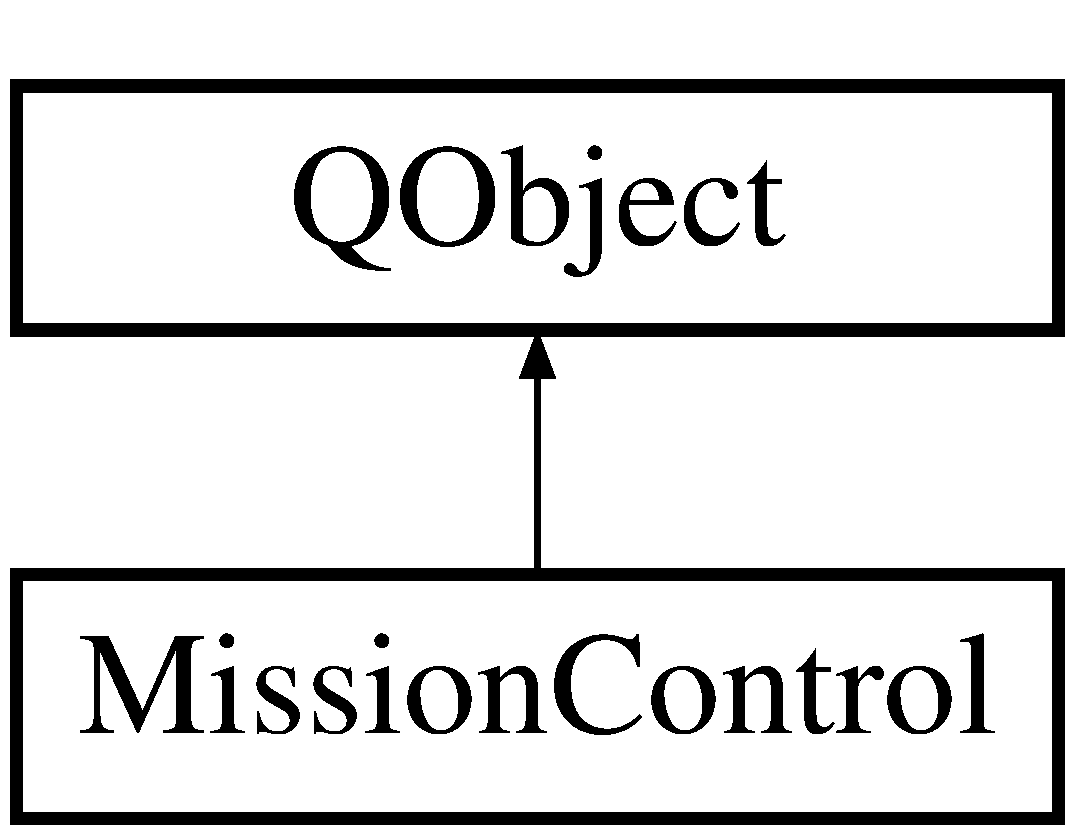
\includegraphics[height=2.000000cm]{d7/dec/a00010}
\end{center}
\end{figure}
\subsection*{Public Slots}
\subsection*{Signals}
\subsection*{Static Public Member Functions}
\subsection*{Private Member Functions}
\subsection*{Private Attributes}
\subsection*{Static Private Attributes}


\subsection{Detailed Description}


\subsection{Constructor \& Destructor Documentation}
\hypertarget{a00010_a4d1fa31327a8451df46c12f7f4a152a4}{\index{Mission\-Control@{Mission\-Control}!Mission\-Control@{Mission\-Control}}
\index{Mission\-Control@{Mission\-Control}!MissionControl@{Mission\-Control}}
\subsubsection[{Mission\-Control}]{\setlength{\rightskip}{0pt plus 5cm}{\bf Mission\-Control} (
\begin{DoxyParamCaption}
{}
\end{DoxyParamCaption}
)\hspace{0.3cm}{\ttfamily [private]}}}\label{a00010_a4d1fa31327a8451df46c12f7f4a152a4}


Constructor. 


\begin{DoxyParams}{Parameters}
{\em none} & \\
\hline
\end{DoxyParams}

\begin{DoxyExceptions}{Exceptions}
{\em none} & \\
\hline
\end{DoxyExceptions}
\begin{DoxyReturn}{Returns}
\hyperlink{a00010}{Mission\-Control} instance 
\end{DoxyReturn}

\begin{DoxyCode}
6 \{
7         \textcolor{comment}{//m\_pPlan = new FlightPlan();}
8         \textcolor{comment}{//m\_pMap = new Map();}
9         \textcolor{comment}{//m\_pMap->setFlightPlan(m\_pPlan);}
10 
11     \hyperlink{a00010_ab3860e046790d0106c5c59d2947c4a24}{m\_pLaunchTimer}.setInterval(1000);
12 
13     connect(\hyperlink{a00001_afebd43c1f2afd7ec0eb35f99e50f0964}{CommunicationControl::getInstance}(), SIGNAL(XBeeStatus(\textcolor{keywordtype}{bool})),
       \textcolor{keyword}{this}, SLOT(\hyperlink{a00010_af5f2c7705408cb9400ff6f2d64eabf26}{updateXBee}(\textcolor{keywordtype}{bool})));
14     connect(\hyperlink{a00011_a81bd14f0b39bba2433355ec26f833270}{PeripheralController::getInstance}(), SIGNAL(directInputProblem
      ()), \textcolor{keyword}{this}, SIGNAL(\hyperlink{a00010_a1ce8df6c21f65fcfbeb3f6852600349e}{directXProblem}()));
15     connect(\hyperlink{a00011_a81bd14f0b39bba2433355ec26f833270}{PeripheralController::getInstance}(), SIGNAL(dataFormatProblem(
      )), \textcolor{keyword}{this}, SIGNAL(\hyperlink{a00010_a1ce8df6c21f65fcfbeb3f6852600349e}{directXProblem}()));
16     connect(\hyperlink{a00011_a81bd14f0b39bba2433355ec26f833270}{PeripheralController::getInstance}(), SIGNAL(deviceEnumProblem(
      )), \textcolor{keyword}{this}, SIGNAL(\hyperlink{a00010_a1ce8df6c21f65fcfbeb3f6852600349e}{directXProblem}()));
17     connect(\hyperlink{a00011_a81bd14f0b39bba2433355ec26f833270}{PeripheralController::getInstance}(), SIGNAL(joystickProblem())
      , \textcolor{keyword}{this}, SIGNAL(\hyperlink{a00010_acda62f445580e9296041e59a2d81fc77}{controllerProblem}()));
18     connect(\hyperlink{a00011_a81bd14f0b39bba2433355ec26f833270}{PeripheralController::getInstance}(), SIGNAL(noJoystick()), \textcolor{keyword}{
      this}, SIGNAL(\hyperlink{a00010_acda62f445580e9296041e59a2d81fc77}{controllerProblem}()));
19     connect(\hyperlink{a00011_a81bd14f0b39bba2433355ec26f833270}{PeripheralController::getInstance}(), SIGNAL(
      \hyperlink{a00010_a35163b56af81dc0f09dc69e92161f4b9}{controllerConnected}()), \textcolor{keyword}{this}, SIGNAL(\hyperlink{a00010_a35163b56af81dc0f09dc69e92161f4b9}{controllerConnected}()));
20 
21     connect(\hyperlink{a00001_afebd43c1f2afd7ec0eb35f99e50f0964}{CommunicationControl::getInstance}(), SIGNAL(geolocation(\textcolor{keywordtype}{double}
      , \textcolor{keywordtype}{double}, \textcolor{keywordtype}{double}, \textcolor{keywordtype}{double})), 
22         \hyperlink{a00012_a40277d38c94caf6125045994ba06f18f}{RPA::getInstance}(), SLOT(geolocation(\textcolor{keywordtype}{double}, \textcolor{keywordtype}{double}, \textcolor{keywordtype}{double}, \textcolor{keywordtype}{double})));
23     connect(\hyperlink{a00001_afebd43c1f2afd7ec0eb35f99e50f0964}{CommunicationControl::getInstance}(), SIGNAL(updateHeading(\textcolor{keywordtype}{
      double})), \hyperlink{a00012_a40277d38c94caf6125045994ba06f18f}{RPA::getInstance}(), SLOT(updateHeading(\textcolor{keywordtype}{double})));
24     connect(\hyperlink{a00001_afebd43c1f2afd7ec0eb35f99e50f0964}{CommunicationControl::getInstance}(), SIGNAL(updateHeight(\textcolor{keywordtype}{
      double})), \hyperlink{a00012_a40277d38c94caf6125045994ba06f18f}{RPA::getInstance}(), SLOT(updateHeight(\textcolor{keywordtype}{double})));
25     connect(\hyperlink{a00001_afebd43c1f2afd7ec0eb35f99e50f0964}{CommunicationControl::getInstance}(), SIGNAL(updateGPSQuality(\textcolor{keywordtype}{
      int})), \textcolor{keyword}{this}, SLOT(\hyperlink{a00010_ae5330168c77c9c4d13fba5b918845ef7}{updateGPS}(\textcolor{keywordtype}{int})));
26     connect(\hyperlink{a00001_afebd43c1f2afd7ec0eb35f99e50f0964}{CommunicationControl::getInstance}(), SIGNAL(
      \hyperlink{a00010_afa417655857cee8564cd3f54b1491e98}{batteryLevel}(\textcolor{keywordtype}{double})), \textcolor{keyword}{this}, SLOT(\hyperlink{a00010_a80fb0b930e406eedf15162edccc726c3}{updateBattery}(\textcolor{keywordtype}{double})));
27     connect(\hyperlink{a00001_afebd43c1f2afd7ec0eb35f99e50f0964}{CommunicationControl::getInstance}(), SIGNAL(updateStatus(\textcolor{keywordtype}{short}
      )), \textcolor{keyword}{this}, SLOT(\hyperlink{a00010_aaf70dd1f6eda48599f92fe2c4426006b}{updateRadiocommand}(\textcolor{keywordtype}{short})));
28     connect(\hyperlink{a00001_afebd43c1f2afd7ec0eb35f99e50f0964}{CommunicationControl::getInstance}(), SIGNAL(
      \hyperlink{a00010_a5f730a9a91784cbf28d39ab22e4d7fec}{inFlight}(\textcolor{keywordtype}{char})), \textcolor{keyword}{this}, SLOT(\hyperlink{a00010_a5f730a9a91784cbf28d39ab22e4d7fec}{inFlight}(\textcolor{keywordtype}{char})));
29     connect(\hyperlink{a00001_afebd43c1f2afd7ec0eb35f99e50f0964}{CommunicationControl::getInstance}(), SIGNAL(waypointNAVInfo(\textcolor{keywordtype}{
      char}, \textcolor{keywordtype}{short}, \textcolor{keywordtype}{short})), 
30         \textcolor{keyword}{this}, SLOT(\hyperlink{a00010_ab3cda15293ced458cbd11c5740c1c099}{updateNAV}(\textcolor{keywordtype}{char}, \textcolor{keywordtype}{short}, \textcolor{keywordtype}{short})));
31     connect(\hyperlink{a00001_afebd43c1f2afd7ec0eb35f99e50f0964}{CommunicationControl::getInstance}(), SIGNAL(
      \hyperlink{a00010_a30bbdc9e8db693b8e568e732fe8bca2e}{rcData}(\textcolor{keywordtype}{short}, \textcolor{keywordtype}{short}, \textcolor{keywordtype}{short}, \textcolor{keywordtype}{short}, \textcolor{keywordtype}{short}, \textcolor{keywordtype}{short}, \textcolor{keywordtype}{char})), 
32         \textcolor{keyword}{this}, SLOT(\hyperlink{a00010_a30bbdc9e8db693b8e568e732fe8bca2e}{rcData}(\textcolor{keywordtype}{short}, \textcolor{keywordtype}{short}, \textcolor{keywordtype}{short}, \textcolor{keywordtype}{short}, \textcolor{keywordtype}{short}, \textcolor{keywordtype}{short}, \textcolor{keywordtype}{char})));
33 
34     connect(\hyperlink{a00012_a40277d38c94caf6125045994ba06f18f}{RPA::getInstance}(), SIGNAL(positionChanged()), \textcolor{keyword}{this}, SLOT(
      \hyperlink{a00010_a161bfdf95298fba69f2227c64a1cbc4c}{updateDigression}()));
35     connect(&\hyperlink{a00010_aa2212ccd53682c3c29395c0012e88979}{m\_pWaypointTimer}, SIGNAL(timeout()), \textcolor{keyword}{this}, SLOT(
      \hyperlink{a00010_a2d1e5a21fd2b1b542b454f72c6fe5bf3}{sendWaypoint}()));
36     connect(&\hyperlink{a00010_ab3860e046790d0106c5c59d2947c4a24}{m\_pLaunchTimer}, SIGNAL(timeout()), \textcolor{keyword}{this}, SIGNAL(
      \hyperlink{a00010_a38513372e1af4752cee2e2d046c98821}{sendLaunch}()));
37 
38     connect(\hyperlink{a00001_afebd43c1f2afd7ec0eb35f99e50f0964}{CommunicationControl::getInstance}(), SIGNAL(displayAck(\textcolor{keywordtype}{char}*))
      , \textcolor{keyword}{this}, SLOT(\hyperlink{a00010_ad15969fb4bfd40eedb8ceaa6c7a8d1f4}{acknowledge}(\textcolor{keywordtype}{char}*)));
39     connect(\textcolor{keyword}{this}, SIGNAL(\hyperlink{a00010_a38513372e1af4752cee2e2d046c98821}{sendLaunch}()), 
      \hyperlink{a00001_afebd43c1f2afd7ec0eb35f99e50f0964}{CommunicationControl::getInstance}(), SIGNAL(
      \hyperlink{a00010_a38513372e1af4752cee2e2d046c98821}{sendLaunch}()));
40     connect(\textcolor{keyword}{this}, SIGNAL(\hyperlink{a00010_a44769de90c2ec83d360149f4b36ea8da}{move}(\textcolor{keywordtype}{double}, \textcolor{keywordtype}{double}, \textcolor{keywordtype}{double}, \textcolor{keywordtype}{double})), 
      \hyperlink{a00001_afebd43c1f2afd7ec0eb35f99e50f0964}{CommunicationControl::getInstance}(), 
41         SIGNAL(sendMove(\textcolor{keywordtype}{double}, \textcolor{keywordtype}{double}, \textcolor{keywordtype}{double}, \textcolor{keywordtype}{double})));
42 
43     \hyperlink{a00010_a093bf32870b9511dce24b7c98b420e9d}{m\_bFirstWaypoint} = \textcolor{keyword}{true};
44     \hyperlink{a00010_ae57780eab0475346a816a8e16e291cd7}{m\_bNextSent} = \textcolor{keyword}{false};
45     \hyperlink{a00010_a23791e7a57e50ca179b551e458922309}{m\_bFPLaunched} = \textcolor{keyword}{false};
46     \hyperlink{a00010_ae0092dd7bee4055937aafc0f9c9eeb17}{m\_bFirstRC} = \textcolor{keyword}{true};
47 \}
\end{DoxyCode}
\hypertarget{a00010_a6841d96310bc959e9bed4f06e0c258dd}{\index{Mission\-Control@{Mission\-Control}!$\sim$\-Mission\-Control@{$\sim$\-Mission\-Control}}
\index{$\sim$\-Mission\-Control@{$\sim$\-Mission\-Control}!MissionControl@{Mission\-Control}}
\subsubsection[{$\sim$\-Mission\-Control}]{\setlength{\rightskip}{0pt plus 5cm}$\sim${\bf Mission\-Control} (
\begin{DoxyParamCaption}
{}
\end{DoxyParamCaption}
)\hspace{0.3cm}{\ttfamily [private]}}}\label{a00010_a6841d96310bc959e9bed4f06e0c258dd}


Destructor. 


\begin{DoxyParams}{Parameters}
{\em none} & \\
\hline
\end{DoxyParams}

\begin{DoxyExceptions}{Exceptions}
{\em none} & \\
\hline
\end{DoxyExceptions}
\begin{DoxyReturn}{Returns}
none 
\end{DoxyReturn}

\begin{DoxyCode}
59 \{
60 \}
\end{DoxyCode}


\subsection{Member Function Documentation}
\hypertarget{a00010_ad15969fb4bfd40eedb8ceaa6c7a8d1f4}{\index{Mission\-Control@{Mission\-Control}!acknowledge@{acknowledge}}
\index{acknowledge@{acknowledge}!MissionControl@{Mission\-Control}}
\subsubsection[{acknowledge}]{\setlength{\rightskip}{0pt plus 5cm}void acknowledge (
\begin{DoxyParamCaption}
\item[{char $\ast$}]{m\-\_\-p\-Ack}
\end{DoxyParamCaption}
)\hspace{0.3cm}{\ttfamily [slot]}}}\label{a00010_ad15969fb4bfd40eedb8ceaa6c7a8d1f4}


Receive M\-U\-A\-V acknowledge. 


\begin{DoxyParams}{Parameters}
{\em m\-\_\-p\-Ack} & acknowledge string char$\ast$ \\
\hline
\end{DoxyParams}

\begin{DoxyExceptions}{Exceptions}
{\em none} & \\
\hline
\end{DoxyExceptions}
\begin{DoxyReturn}{Returns}
none 
\end{DoxyReturn}

\begin{DoxyCode}
185 \{
186     QString ack(m\_pAck);
187 
188     \textcolor{keywordflow}{if} (ack == WAYPOINT\_ACK)
189     \{
190         \hyperlink{a00010_aa2212ccd53682c3c29395c0012e88979}{m\_pWaypointTimer}.stop();
191     \}
192     \textcolor{keywordflow}{else} \textcolor{keywordflow}{if} (ack == DEFINE\_HOME\_ACK)
193     \{
194         \hyperlink{a00010_ab3860e046790d0106c5c59d2947c4a24}{m\_pLaunchTimer}.stop();
195     \}
196 \}
\end{DoxyCode}
\hypertarget{a00010_a48a7112262ba65d18ca31b7419a81ac1}{\index{Mission\-Control@{Mission\-Control}!add\-Mark@{add\-Mark}}
\index{add\-Mark@{add\-Mark}!MissionControl@{Mission\-Control}}
\subsubsection[{add\-Mark}]{\setlength{\rightskip}{0pt plus 5cm}void add\-Mark (
\begin{DoxyParamCaption}
{}
\end{DoxyParamCaption}
)\hspace{0.3cm}{\ttfamily [slot]}}}\label{a00010_a48a7112262ba65d18ca31b7419a81ac1}

\begin{DoxyCode}
313 \{
314         \textcolor{comment}{//Waypoint* pWaypoint = new Waypoint(RPA::getInstance()->getCoordinates(),
       RPA::getInstance()->getHeight());}
315         \textcolor{comment}{//pWaypoint->setNumber(MissionControl::getInstance()->getPlan()->getWaypointList().size() +}
316         \textcolor{comment}{//  MissionControl::getInstance()->getPlan()->getMarkList().size() + 1);}
317         \textcolor{comment}{//pWaypoint->setAction(new Action(GOTO));}
318 
319         \textcolor{comment}{//MissionControl::getInstance()->getPlan()->addMark(pWaypoint);}
320 \}
\end{DoxyCode}
\hypertarget{a00010_afa417655857cee8564cd3f54b1491e98}{\index{Mission\-Control@{Mission\-Control}!battery\-Level@{battery\-Level}}
\index{battery\-Level@{battery\-Level}!MissionControl@{Mission\-Control}}
\subsubsection[{battery\-Level}]{\setlength{\rightskip}{0pt plus 5cm}void battery\-Level (
\begin{DoxyParamCaption}
\item[{double}]{p\-\_\-p\-Value}
\end{DoxyParamCaption}
)\hspace{0.3cm}{\ttfamily [signal]}}}\label{a00010_afa417655857cee8564cd3f54b1491e98}


Battery level. 


\begin{DoxyParams}{Parameters}
{\em none} & \\
\hline
\end{DoxyParams}

\begin{DoxyExceptions}{Exceptions}
{\em none} & \\
\hline
\end{DoxyExceptions}
\begin{DoxyReturn}{Returns}
none 
\end{DoxyReturn}
\hypertarget{a00010_ab84abdda4808cd9ca3f154e9d8f0b133}{\index{Mission\-Control@{Mission\-Control}!cannot\-Launch\-F\-P@{cannot\-Launch\-F\-P}}
\index{cannot\-Launch\-F\-P@{cannot\-Launch\-F\-P}!MissionControl@{Mission\-Control}}
\subsubsection[{cannot\-Launch\-F\-P}]{\setlength{\rightskip}{0pt plus 5cm}void cannot\-Launch\-F\-P (
\begin{DoxyParamCaption}
\item[{bool}]{p\-\_\-b\-Battery, }
\item[{bool}]{p\-\_\-b\-G\-P\-S, }
\item[{bool}]{p\-\_\-b\-X\-Bee, }
\item[{bool}]{p\-\_\-b\-Status, }
\item[{bool}]{p\-\_\-b\-Flight\-Plan, }
\item[{bool}]{p\-\_\-b\-Engine}
\end{DoxyParamCaption}
)\hspace{0.3cm}{\ttfamily [signal]}}}\label{a00010_ab84abdda4808cd9ca3f154e9d8f0b133}


Cannot launch flight plan event. 


\begin{DoxyParams}{Parameters}
{\em p\-\_\-b\-Battery} & battery level above low bool \\
\hline
{\em p\-\_\-b\-G\-P\-S} & enough satellites bool \\
\hline
{\em p\-\_\-b\-X\-Bee} & link through X\-Bee bool \\
\hline
{\em p\-\_\-b\-Status} & M\-U\-A\-V in G\-P\-S mode bool \\
\hline
{\em p\-\_\-b\-Flight\-Plan} & flight plan loaded bool \\
\hline
{\em p\-\_\-b\-Engine} & engines started bool \\
\hline
\end{DoxyParams}

\begin{DoxyExceptions}{Exceptions}
{\em none} & \\
\hline
\end{DoxyExceptions}
\begin{DoxyReturn}{Returns}
none 
\end{DoxyReturn}
\hypertarget{a00010_a35163b56af81dc0f09dc69e92161f4b9}{\index{Mission\-Control@{Mission\-Control}!controller\-Connected@{controller\-Connected}}
\index{controller\-Connected@{controller\-Connected}!MissionControl@{Mission\-Control}}
\subsubsection[{controller\-Connected}]{\setlength{\rightskip}{0pt plus 5cm}void controller\-Connected (
\begin{DoxyParamCaption}
{}
\end{DoxyParamCaption}
)\hspace{0.3cm}{\ttfamily [signal]}}}\label{a00010_a35163b56af81dc0f09dc69e92161f4b9}


Controller connected. 


\begin{DoxyParams}{Parameters}
{\em none} & \\
\hline
\end{DoxyParams}

\begin{DoxyExceptions}{Exceptions}
{\em none} & \\
\hline
\end{DoxyExceptions}
\begin{DoxyReturn}{Returns}
none 
\end{DoxyReturn}
\hypertarget{a00010_acda62f445580e9296041e59a2d81fc77}{\index{Mission\-Control@{Mission\-Control}!controller\-Problem@{controller\-Problem}}
\index{controller\-Problem@{controller\-Problem}!MissionControl@{Mission\-Control}}
\subsubsection[{controller\-Problem}]{\setlength{\rightskip}{0pt plus 5cm}void controller\-Problem (
\begin{DoxyParamCaption}
{}
\end{DoxyParamCaption}
)\hspace{0.3cm}{\ttfamily [signal]}}}\label{a00010_acda62f445580e9296041e59a2d81fc77}


Problem with the game controller. 


\begin{DoxyParams}{Parameters}
{\em none} & \\
\hline
\end{DoxyParams}

\begin{DoxyExceptions}{Exceptions}
{\em none} & \\
\hline
\end{DoxyExceptions}
\begin{DoxyReturn}{Returns}
none 
\end{DoxyReturn}
\hypertarget{a00010_ab767c53cb52cd34736797a11063e05b7}{\index{Mission\-Control@{Mission\-Control}!digression@{digression}}
\index{digression@{digression}!MissionControl@{Mission\-Control}}
\subsubsection[{digression}]{\setlength{\rightskip}{0pt plus 5cm}void digression (
\begin{DoxyParamCaption}
\item[{double}]{p\-\_\-p\-Value}
\end{DoxyParamCaption}
)\hspace{0.3cm}{\ttfamily [signal]}}}\label{a00010_ab767c53cb52cd34736797a11063e05b7}


Digression value. 


\begin{DoxyParams}{Parameters}
{\em none} & \\
\hline
\end{DoxyParams}

\begin{DoxyExceptions}{Exceptions}
{\em none} & \\
\hline
\end{DoxyExceptions}
\begin{DoxyReturn}{Returns}
none 
\end{DoxyReturn}
\hypertarget{a00010_a1ce8df6c21f65fcfbeb3f6852600349e}{\index{Mission\-Control@{Mission\-Control}!direct\-X\-Problem@{direct\-X\-Problem}}
\index{direct\-X\-Problem@{direct\-X\-Problem}!MissionControl@{Mission\-Control}}
\subsubsection[{direct\-X\-Problem}]{\setlength{\rightskip}{0pt plus 5cm}void direct\-X\-Problem (
\begin{DoxyParamCaption}
{}
\end{DoxyParamCaption}
)\hspace{0.3cm}{\ttfamily [signal]}}}\label{a00010_a1ce8df6c21f65fcfbeb3f6852600349e}


Direct X problem. 


\begin{DoxyParams}{Parameters}
{\em none} & \\
\hline
\end{DoxyParams}

\begin{DoxyExceptions}{Exceptions}
{\em none} & \\
\hline
\end{DoxyExceptions}
\begin{DoxyReturn}{Returns}
none 
\end{DoxyReturn}
\hypertarget{a00010_a6663cf1e20c2f8162d29d31c8f6324e6}{\index{Mission\-Control@{Mission\-Control}!down@{down}}
\index{down@{down}!MissionControl@{Mission\-Control}}
\subsubsection[{down}]{\setlength{\rightskip}{0pt plus 5cm}void down (
\begin{DoxyParamCaption}
{}
\end{DoxyParamCaption}
)\hspace{0.3cm}{\ttfamily [slot]}}}\label{a00010_a6663cf1e20c2f8162d29d31c8f6324e6}


Decrease altitude command. 


\begin{DoxyParams}{Parameters}
{\em none} & \\
\hline
\end{DoxyParams}

\begin{DoxyExceptions}{Exceptions}
{\em none} & \\
\hline
\end{DoxyExceptions}
\begin{DoxyReturn}{Returns}
none 
\end{DoxyReturn}

\begin{DoxyCode}
308 \{
309     emit \hyperlink{a00010_a44769de90c2ec83d360149f4b36ea8da}{move}(0, 0, \hyperlink{a00012_a40277d38c94caf6125045994ba06f18f}{RPA::getInstance}()->getAltitude() - 10, 
      \hyperlink{a00012_a40277d38c94caf6125045994ba06f18f}{RPA::getInstance}()->getHeading());
310 \}
\end{DoxyCode}
\hypertarget{a00010_a65673b3acf5f5593d90cc2cb8f1b78f9}{\index{Mission\-Control@{Mission\-Control}!end\-Flight\-Plan@{end\-Flight\-Plan}}
\index{end\-Flight\-Plan@{end\-Flight\-Plan}!MissionControl@{Mission\-Control}}
\subsubsection[{end\-Flight\-Plan}]{\setlength{\rightskip}{0pt plus 5cm}void end\-Flight\-Plan (
\begin{DoxyParamCaption}
{}
\end{DoxyParamCaption}
)\hspace{0.3cm}{\ttfamily [signal]}}}\label{a00010_a65673b3acf5f5593d90cc2cb8f1b78f9}


End of flight plan event. 


\begin{DoxyParams}{Parameters}
{\em none} & \\
\hline
\end{DoxyParams}

\begin{DoxyExceptions}{Exceptions}
{\em none} & \\
\hline
\end{DoxyExceptions}
\begin{DoxyReturn}{Returns}
none 
\end{DoxyReturn}
\hypertarget{a00010_a03472851679eb075b2fad51e1ef61f2e}{\index{Mission\-Control@{Mission\-Control}!flight\-Plan\-Launched@{flight\-Plan\-Launched}}
\index{flight\-Plan\-Launched@{flight\-Plan\-Launched}!MissionControl@{Mission\-Control}}
\subsubsection[{flight\-Plan\-Launched}]{\setlength{\rightskip}{0pt plus 5cm}void flight\-Plan\-Launched (
\begin{DoxyParamCaption}
{}
\end{DoxyParamCaption}
)\hspace{0.3cm}{\ttfamily [signal]}}}\label{a00010_a03472851679eb075b2fad51e1ef61f2e}


Flight plan launched acknowledge. 


\begin{DoxyParams}{Parameters}
{\em none} & \\
\hline
\end{DoxyParams}

\begin{DoxyExceptions}{Exceptions}
{\em none} & \\
\hline
\end{DoxyExceptions}
\begin{DoxyReturn}{Returns}
none 
\end{DoxyReturn}
\hypertarget{a00010_a0ec34c9f235c87920390dd2425a8a162}{\index{Mission\-Control@{Mission\-Control}!get\-Instance@{get\-Instance}}
\index{get\-Instance@{get\-Instance}!MissionControl@{Mission\-Control}}
\subsubsection[{get\-Instance}]{\setlength{\rightskip}{0pt plus 5cm}{\bf Mission\-Control} $\ast$ get\-Instance (
\begin{DoxyParamCaption}
{}
\end{DoxyParamCaption}
)\hspace{0.3cm}{\ttfamily [static]}}}\label{a00010_a0ec34c9f235c87920390dd2425a8a162}


\hyperlink{a00010}{Mission\-Control} lone instance getter. 


\begin{DoxyParams}{Parameters}
{\em none} & \\
\hline
\end{DoxyParams}

\begin{DoxyExceptions}{Exceptions}
{\em none} & \\
\hline
\end{DoxyExceptions}
\begin{DoxyReturn}{Returns}
lone instance Mission\-Control$\ast$ 
\end{DoxyReturn}

\begin{DoxyCode}
63 \{
64     \textcolor{keywordflow}{if} (\hyperlink{a00010_a05b55b7963750cd3d108e76c1250d477}{singleton} == NULL)
65     \{
66         \hyperlink{a00010_a05b55b7963750cd3d108e76c1250d477}{singleton} = \textcolor{keyword}{new} \hyperlink{a00010_a4d1fa31327a8451df46c12f7f4a152a4}{MissionControl}();
67     \}
68 
69     \textcolor{keywordflow}{return} \hyperlink{a00010_a05b55b7963750cd3d108e76c1250d477}{singleton};
70 \}
\end{DoxyCode}
\hypertarget{a00010_ab333658b290f86625babfe23d9148bc5}{\index{Mission\-Control@{Mission\-Control}!G\-P\-S\-Level@{G\-P\-S\-Level}}
\index{G\-P\-S\-Level@{G\-P\-S\-Level}!MissionControl@{Mission\-Control}}
\subsubsection[{G\-P\-S\-Level}]{\setlength{\rightskip}{0pt plus 5cm}void G\-P\-S\-Level (
\begin{DoxyParamCaption}
\item[{int}]{p\-\_\-p\-Value}
\end{DoxyParamCaption}
)\hspace{0.3cm}{\ttfamily [signal]}}}\label{a00010_ab333658b290f86625babfe23d9148bc5}


G\-P\-S reception level. 


\begin{DoxyParams}{Parameters}
{\em none} & \\
\hline
\end{DoxyParams}

\begin{DoxyExceptions}{Exceptions}
{\em none} & \\
\hline
\end{DoxyExceptions}
\begin{DoxyReturn}{Returns}
none 
\end{DoxyReturn}
\hypertarget{a00010_a5f730a9a91784cbf28d39ab22e4d7fec}{\index{Mission\-Control@{Mission\-Control}!in\-Flight@{in\-Flight}}
\index{in\-Flight@{in\-Flight}!MissionControl@{Mission\-Control}}
\subsubsection[{in\-Flight}]{\setlength{\rightskip}{0pt plus 5cm}void in\-Flight (
\begin{DoxyParamCaption}
\item[{char}]{p\-\_\-c\-Value}
\end{DoxyParamCaption}
)\hspace{0.3cm}{\ttfamily [slot]}}}\label{a00010_a5f730a9a91784cbf28d39ab22e4d7fec}


Define if the M\-U\-A\-V has its engines started. 


\begin{DoxyParams}{Parameters}
{\em none} & \\
\hline
\end{DoxyParams}

\begin{DoxyExceptions}{Exceptions}
{\em none} & \\
\hline
\end{DoxyExceptions}
\begin{DoxyReturn}{Returns}
none 
\end{DoxyReturn}

\begin{DoxyCode}
268 \{
269     \hyperlink{a00010_a4becef68fb68fff5f845aff02c8a4b7a}{m\_cEngine} = p\_cValue;
270 \}
\end{DoxyCode}
\hypertarget{a00010_aae9d52caad9fb2892deeb25596cfd2ab}{\index{Mission\-Control@{Mission\-Control}!kill@{kill}}
\index{kill@{kill}!MissionControl@{Mission\-Control}}
\subsubsection[{kill}]{\setlength{\rightskip}{0pt plus 5cm}void kill (
\begin{DoxyParamCaption}
{}
\end{DoxyParamCaption}
)\hspace{0.3cm}{\ttfamily [static]}}}\label{a00010_aae9d52caad9fb2892deeb25596cfd2ab}


Instance killer. 


\begin{DoxyParams}{Parameters}
{\em none} & \\
\hline
\end{DoxyParams}

\begin{DoxyExceptions}{Exceptions}
{\em none} & \\
\hline
\end{DoxyExceptions}
\begin{DoxyReturn}{Returns}
none 
\end{DoxyReturn}

\begin{DoxyCode}
50 \{
51     \textcolor{keywordflow}{if} (\hyperlink{a00010_a05b55b7963750cd3d108e76c1250d477}{singleton} != NULL)
52     \{
53         \textcolor{keyword}{delete} \hyperlink{a00010_a05b55b7963750cd3d108e76c1250d477}{singleton};
54         \hyperlink{a00010_a05b55b7963750cd3d108e76c1250d477}{singleton} = NULL;
55     \}
56 \}
\end{DoxyCode}
\hypertarget{a00010_aa638de738a43a5d84d5cc765a9ca87c5}{\index{Mission\-Control@{Mission\-Control}!launch\-Flight\-Plan@{launch\-Flight\-Plan}}
\index{launch\-Flight\-Plan@{launch\-Flight\-Plan}!MissionControl@{Mission\-Control}}
\subsubsection[{launch\-Flight\-Plan}]{\setlength{\rightskip}{0pt plus 5cm}void launch\-Flight\-Plan (
\begin{DoxyParamCaption}
{}
\end{DoxyParamCaption}
)\hspace{0.3cm}{\ttfamily [slot]}}}\label{a00010_aa638de738a43a5d84d5cc765a9ca87c5}


Launch the flight plan. 


\begin{DoxyParams}{Parameters}
{\em none} & \\
\hline
\end{DoxyParams}

\begin{DoxyExceptions}{Exceptions}
{\em indicate} & if cannot launch (bad parameters) \\
\hline
\end{DoxyExceptions}
\begin{DoxyReturn}{Returns}
none 
\end{DoxyReturn}

\begin{DoxyCode}
199 \{
200         \textcolor{comment}{//bool bFlightPlanDefined = m\_pPlan->getWaypointList().size() != 0;}
201 
202         \textcolor{comment}{//if (m\_dBattery > batteryVeryLow && /*m\_nGPS > GPSVeryLow &&*/ m\_bXBee}
203         \textcolor{comment}{//  && (m\_nStatus & GPS) && bFlightPlanDefined && m\_cEngine == 1)}
204     \textcolor{keywordflow}{if} (\textcolor{keyword}{true})
205     \{
206         \hyperlink{a00010_a23791e7a57e50ca179b551e458922309}{m\_bFPLaunched} = \textcolor{keyword}{true};
207         emit \hyperlink{a00010_a03472851679eb075b2fad51e1ef61f2e}{flightPlanLaunched}();
208     \}
209     \textcolor{keywordflow}{else}
210     \{
211                 \textcolor{comment}{//emit cannotLaunchFP(m\_dBattery > batteryVeryLow, m\_nGPS > GPSVeryLow, m\_bXBee,}
212                 \textcolor{comment}{//  m\_nStatus & GPS, bFlightPlanDefined, m\_cEngine == 1);}
213     \}
214 \}
\end{DoxyCode}
\hypertarget{a00010_a44769de90c2ec83d360149f4b36ea8da}{\index{Mission\-Control@{Mission\-Control}!move@{move}}
\index{move@{move}!MissionControl@{Mission\-Control}}
\subsubsection[{move}]{\setlength{\rightskip}{0pt plus 5cm}void move (
\begin{DoxyParamCaption}
\item[{double}]{x, }
\item[{double}]{y, }
\item[{double}]{z, }
\item[{double}]{yaw}
\end{DoxyParamCaption}
)\hspace{0.3cm}{\ttfamily [signal]}}}\label{a00010_a44769de90c2ec83d360149f4b36ea8da}


\hyperlink{a00017}{Waypoint} to send. 


\begin{DoxyParams}{Parameters}
{\em x} & in meters double \\
\hline
{\em y} & in meters double \\
\hline
{\em z} & altitude double \\
\hline
{\em yaw} & heading double \\
\hline
\end{DoxyParams}

\begin{DoxyExceptions}{Exceptions}
{\em none} & \\
\hline
\end{DoxyExceptions}
\begin{DoxyReturn}{Returns}
none 
\end{DoxyReturn}
\hypertarget{a00010_a39321c04c34c4c2e46ed14803bdddd39}{\index{Mission\-Control@{Mission\-Control}!move\-Backward@{move\-Backward}}
\index{move\-Backward@{move\-Backward}!MissionControl@{Mission\-Control}}
\subsubsection[{move\-Backward}]{\setlength{\rightskip}{0pt plus 5cm}void move\-Backward (
\begin{DoxyParamCaption}
{}
\end{DoxyParamCaption}
)\hspace{0.3cm}{\ttfamily [slot]}}}\label{a00010_a39321c04c34c4c2e46ed14803bdddd39}


Move backward command. 


\begin{DoxyParams}{Parameters}
{\em none} & \\
\hline
\end{DoxyParams}

\begin{DoxyExceptions}{Exceptions}
{\em none} & \\
\hline
\end{DoxyExceptions}
\begin{DoxyReturn}{Returns}
none 
\end{DoxyReturn}

\begin{DoxyCode}
278 \{
279     emit \hyperlink{a00010_a44769de90c2ec83d360149f4b36ea8da}{move}(-10, 0, \hyperlink{a00012_a40277d38c94caf6125045994ba06f18f}{RPA::getInstance}()->getAltitude(), 
      \hyperlink{a00012_a40277d38c94caf6125045994ba06f18f}{RPA::getInstance}()->getHeading());
280 \}
\end{DoxyCode}
\hypertarget{a00010_a618d986e214be5b102686274ac420be0}{\index{Mission\-Control@{Mission\-Control}!move\-Forward@{move\-Forward}}
\index{move\-Forward@{move\-Forward}!MissionControl@{Mission\-Control}}
\subsubsection[{move\-Forward}]{\setlength{\rightskip}{0pt plus 5cm}void move\-Forward (
\begin{DoxyParamCaption}
{}
\end{DoxyParamCaption}
)\hspace{0.3cm}{\ttfamily [slot]}}}\label{a00010_a618d986e214be5b102686274ac420be0}


Move forward command. 


\begin{DoxyParams}{Parameters}
{\em none} & \\
\hline
\end{DoxyParams}

\begin{DoxyExceptions}{Exceptions}
{\em none} & \\
\hline
\end{DoxyExceptions}
\begin{DoxyReturn}{Returns}
none 
\end{DoxyReturn}

\begin{DoxyCode}
273 \{
274     emit \hyperlink{a00010_a44769de90c2ec83d360149f4b36ea8da}{move}(10, 0, \hyperlink{a00012_a40277d38c94caf6125045994ba06f18f}{RPA::getInstance}()->getAltitude(), 
      \hyperlink{a00012_a40277d38c94caf6125045994ba06f18f}{RPA::getInstance}()->getHeading());
275 \}
\end{DoxyCode}
\hypertarget{a00010_a7a5379770a3d9a90ee4d827046d26eb0}{\index{Mission\-Control@{Mission\-Control}!move\-Left@{move\-Left}}
\index{move\-Left@{move\-Left}!MissionControl@{Mission\-Control}}
\subsubsection[{move\-Left}]{\setlength{\rightskip}{0pt plus 5cm}void move\-Left (
\begin{DoxyParamCaption}
{}
\end{DoxyParamCaption}
)\hspace{0.3cm}{\ttfamily [slot]}}}\label{a00010_a7a5379770a3d9a90ee4d827046d26eb0}


Move left command. 


\begin{DoxyParams}{Parameters}
{\em none} & \\
\hline
\end{DoxyParams}

\begin{DoxyExceptions}{Exceptions}
{\em none} & \\
\hline
\end{DoxyExceptions}
\begin{DoxyReturn}{Returns}
none 
\end{DoxyReturn}

\begin{DoxyCode}
283 \{
284     emit \hyperlink{a00010_a44769de90c2ec83d360149f4b36ea8da}{move}(0, 10, \hyperlink{a00012_a40277d38c94caf6125045994ba06f18f}{RPA::getInstance}()->getAltitude(), 
      \hyperlink{a00012_a40277d38c94caf6125045994ba06f18f}{RPA::getInstance}()->getHeading());
285 \}
\end{DoxyCode}
\hypertarget{a00010_a8f1aff0fabeb87f42932d5ce436f4d5c}{\index{Mission\-Control@{Mission\-Control}!move\-Right@{move\-Right}}
\index{move\-Right@{move\-Right}!MissionControl@{Mission\-Control}}
\subsubsection[{move\-Right}]{\setlength{\rightskip}{0pt plus 5cm}void move\-Right (
\begin{DoxyParamCaption}
{}
\end{DoxyParamCaption}
)\hspace{0.3cm}{\ttfamily [slot]}}}\label{a00010_a8f1aff0fabeb87f42932d5ce436f4d5c}


Move right command. 


\begin{DoxyParams}{Parameters}
{\em none} & \\
\hline
\end{DoxyParams}

\begin{DoxyExceptions}{Exceptions}
{\em none} & \\
\hline
\end{DoxyExceptions}
\begin{DoxyReturn}{Returns}
none 
\end{DoxyReturn}

\begin{DoxyCode}
288 \{
289     emit \hyperlink{a00010_a44769de90c2ec83d360149f4b36ea8da}{move}(0, -10, \hyperlink{a00012_a40277d38c94caf6125045994ba06f18f}{RPA::getInstance}()->getAltitude(), 
      \hyperlink{a00012_a40277d38c94caf6125045994ba06f18f}{RPA::getInstance}()->getHeading());
290 \}
\end{DoxyCode}
\hypertarget{a00010_a8fb230ae2937902d2f3f70505b5c08d0}{\index{Mission\-Control@{Mission\-Control}!next\-Waypoint@{next\-Waypoint}}
\index{next\-Waypoint@{next\-Waypoint}!MissionControl@{Mission\-Control}}
\subsubsection[{next\-Waypoint}]{\setlength{\rightskip}{0pt plus 5cm}bool next\-Waypoint (
\begin{DoxyParamCaption}
{}
\end{DoxyParamCaption}
)\hspace{0.3cm}{\ttfamily [slot]}}}\label{a00010_a8fb230ae2937902d2f3f70505b5c08d0}


Next waypoint index increment. 


\begin{DoxyParams}{Parameters}
{\em none} & \\
\hline
\end{DoxyParams}

\begin{DoxyExceptions}{Exceptions}
{\em none} & \\
\hline
\end{DoxyExceptions}
\begin{DoxyReturn}{Returns}
end of flight plan reached 
\end{DoxyReturn}

\begin{DoxyCode}
133 \{
134     \textcolor{keywordtype}{bool} ret = \textcolor{keyword}{false};
135         \textcolor{comment}{//int index = m\_pPlan->getNextWaypointIndex();}
136 
137         \textcolor{comment}{//if (index < m\_pPlan->getWaypointList().size())}
138         \textcolor{keywordflow}{if}(\textcolor{keyword}{true})
139     \{
140         \textcolor{comment}{//  m\_pPlan->setNextWaypointIndex(index + 1);}
141         ret = \textcolor{keyword}{true};
142     \}
143     \textcolor{keywordflow}{else}
144     \{
145         ret = \textcolor{keyword}{false};
146     \}
147 
148         \textcolor{comment}{//m\_pMap->displayWaypoints();}
149     emit \hyperlink{a00010_a5da6fbcca696f2541c3d121ca0fe9e85}{resetWaypointNotification}();
150 
151     \textcolor{keywordflow}{return} ret;
152 \}
\end{DoxyCode}
\hypertarget{a00010_a1d4b9f41f5f619c4ef938ab08265fce4}{\index{Mission\-Control@{Mission\-Control}!pause\-Flight\-Plan@{pause\-Flight\-Plan}}
\index{pause\-Flight\-Plan@{pause\-Flight\-Plan}!MissionControl@{Mission\-Control}}
\subsubsection[{pause\-Flight\-Plan}]{\setlength{\rightskip}{0pt plus 5cm}void pause\-Flight\-Plan (
\begin{DoxyParamCaption}
{}
\end{DoxyParamCaption}
)\hspace{0.3cm}{\ttfamily [slot]}}}\label{a00010_a1d4b9f41f5f619c4ef938ab08265fce4}


Pause flight plan (no reset of next waypoint index) 


\begin{DoxyParams}{Parameters}
{\em none} & \\
\hline
\end{DoxyParams}

\begin{DoxyExceptions}{Exceptions}
{\em none} & \\
\hline
\end{DoxyExceptions}
\begin{DoxyReturn}{Returns}
none 
\end{DoxyReturn}

\begin{DoxyCode}
224 \{
225     \hyperlink{a00010_a23791e7a57e50ca179b551e458922309}{m\_bFPLaunched} = \textcolor{keyword}{false};
226 \}
\end{DoxyCode}
\hypertarget{a00010_a45f0ce9c30deececbfdab8cc03d50eab}{\index{Mission\-Control@{Mission\-Control}!radiocommand\-Connection@{radiocommand\-Connection}}
\index{radiocommand\-Connection@{radiocommand\-Connection}!MissionControl@{Mission\-Control}}
\subsubsection[{radiocommand\-Connection}]{\setlength{\rightskip}{0pt plus 5cm}void radiocommand\-Connection (
\begin{DoxyParamCaption}
\item[{bool}]{p\-\_\-p\-Value}
\end{DoxyParamCaption}
)\hspace{0.3cm}{\ttfamily [signal]}}}\label{a00010_a45f0ce9c30deececbfdab8cc03d50eab}


Radiocommand connection state. 


\begin{DoxyParams}{Parameters}
{\em none} & \\
\hline
\end{DoxyParams}

\begin{DoxyExceptions}{Exceptions}
{\em none} & \\
\hline
\end{DoxyExceptions}
\begin{DoxyReturn}{Returns}
none 
\end{DoxyReturn}
\hypertarget{a00010_a30bbdc9e8db693b8e568e732fe8bca2e}{\index{Mission\-Control@{Mission\-Control}!rc\-Data@{rc\-Data}}
\index{rc\-Data@{rc\-Data}!MissionControl@{Mission\-Control}}
\subsubsection[{rc\-Data}]{\setlength{\rightskip}{0pt plus 5cm}void rc\-Data (
\begin{DoxyParamCaption}
\item[{short}]{p\-\_\-n\-Yaw, }
\item[{short}]{p\-\_\-n\-Pitch, }
\item[{short}]{p\-\_\-n\-Roll, }
\item[{short}]{p\-\_\-n\-Thrust, }
\item[{short}]{p\-\_\-n\-Serial, }
\item[{short}]{p\-\_\-n\-G\-P\-S\-Height\-Control, }
\item[{char}]{p\-\_\-c\-Valid}
\end{DoxyParamCaption}
)\hspace{0.3cm}{\ttfamily [slot]}}}\label{a00010_a30bbdc9e8db693b8e568e732fe8bca2e}


Define if remote control values changed and update them. 


\begin{DoxyParams}{Parameters}
{\em yaw} & short \\
\hline
{\em pitch} & short \\
\hline
{\em roll} & short \\
\hline
{\em thrust} & short \\
\hline
{\em serial} & short \\
\hline
{\em G\-P\-S\-Height\-Control} & short \\
\hline
{\em valid} & char \\
\hline
\end{DoxyParams}

\begin{DoxyExceptions}{Exceptions}
{\em none} & \\
\hline
\end{DoxyExceptions}
\begin{DoxyReturn}{Returns}
none 
\end{DoxyReturn}

\begin{DoxyCode}
241 \{
242     \textcolor{keywordflow}{if} (p\_cValid)
243     \{
244         \textcolor{keywordflow}{if} (!\hyperlink{a00010_ae0092dd7bee4055937aafc0f9c9eeb17}{m\_bFirstRC} && \hyperlink{a00011_a81bd14f0b39bba2433355ec26f833270}{PeripheralController::getInstance}()->
      isMouseMode())
245         \{
246             \textcolor{keywordflow}{if} (\hyperlink{a00010_a3156a3f666d6691390fe845a9c28c40d}{m\_pPreviousYawRC} != p\_nYaw || \hyperlink{a00010_a1c95c212ff083bed4a5ff651e39837de}{m\_pPreviousPitchRC} != 
      p\_nPitch
247                 || \hyperlink{a00010_a1a6d2ee64c0380d556c8d16f21241493}{m\_pPreviousRollRC} != p\_nRoll || 
      \hyperlink{a00010_a5ce9c2712c259fa2004b16421b891b2b}{m\_pPreviousThrustRC} != p\_nThrust
248                 || \hyperlink{a00010_ae4629b3de032de49ef686d0a7fc3904e}{m\_pPreviousSerialRC} != p\_nSerial || 
      \hyperlink{a00010_a9cd9caa80b9e3f0c4c7c89f721fb12ab}{m\_pPreviousGPSHeightControlRC} != p\_nGPSHeightControl)
249             \{
250                 emit \hyperlink{a00010_a2780ef8954a3ec68cdc55d312e2e06ce}{RCDataChanged}();
251 
252                 \hyperlink{a00010_a3156a3f666d6691390fe845a9c28c40d}{m\_pPreviousYawRC} = p\_nYaw;
253                 \hyperlink{a00010_a1c95c212ff083bed4a5ff651e39837de}{m\_pPreviousPitchRC} = p\_nPitch;
254                 \hyperlink{a00010_a1a6d2ee64c0380d556c8d16f21241493}{m\_pPreviousRollRC} = p\_nRoll;
255                 \hyperlink{a00010_a5ce9c2712c259fa2004b16421b891b2b}{m\_pPreviousThrustRC} = p\_nThrust;
256                 \hyperlink{a00010_ae4629b3de032de49ef686d0a7fc3904e}{m\_pPreviousSerialRC} = p\_nSerial;
257                 \hyperlink{a00010_a9cd9caa80b9e3f0c4c7c89f721fb12ab}{m\_pPreviousGPSHeightControlRC} = p\_nGPSHeightControl;
258             \}
259         \}
260         \textcolor{keywordflow}{else}
261         \{
262             \hyperlink{a00010_ae0092dd7bee4055937aafc0f9c9eeb17}{m\_bFirstRC} = \textcolor{keyword}{false};
263         \}
264     \}
265 \}
\end{DoxyCode}
\hypertarget{a00010_a2780ef8954a3ec68cdc55d312e2e06ce}{\index{Mission\-Control@{Mission\-Control}!R\-C\-Data\-Changed@{R\-C\-Data\-Changed}}
\index{R\-C\-Data\-Changed@{R\-C\-Data\-Changed}!MissionControl@{Mission\-Control}}
\subsubsection[{R\-C\-Data\-Changed}]{\setlength{\rightskip}{0pt plus 5cm}void R\-C\-Data\-Changed (
\begin{DoxyParamCaption}
{}
\end{DoxyParamCaption}
)\hspace{0.3cm}{\ttfamily [signal]}}}\label{a00010_a2780ef8954a3ec68cdc55d312e2e06ce}


Remote control values changed. 


\begin{DoxyParams}{Parameters}
{\em none} & \\
\hline
\end{DoxyParams}

\begin{DoxyExceptions}{Exceptions}
{\em none} & \\
\hline
\end{DoxyExceptions}
\begin{DoxyReturn}{Returns}
none 
\end{DoxyReturn}
\hypertarget{a00010_a5da6fbcca696f2541c3d121ca0fe9e85}{\index{Mission\-Control@{Mission\-Control}!reset\-Waypoint\-Notification@{reset\-Waypoint\-Notification}}
\index{reset\-Waypoint\-Notification@{reset\-Waypoint\-Notification}!MissionControl@{Mission\-Control}}
\subsubsection[{reset\-Waypoint\-Notification}]{\setlength{\rightskip}{0pt plus 5cm}void reset\-Waypoint\-Notification (
\begin{DoxyParamCaption}
{}
\end{DoxyParamCaption}
)\hspace{0.3cm}{\ttfamily [signal]}}}\label{a00010_a5da6fbcca696f2541c3d121ca0fe9e85}


Change next waypoint. 


\begin{DoxyParams}{Parameters}
{\em none} & \\
\hline
\end{DoxyParams}

\begin{DoxyExceptions}{Exceptions}
{\em none} & \\
\hline
\end{DoxyExceptions}
\begin{DoxyReturn}{Returns}
none 
\end{DoxyReturn}
\hypertarget{a00010_a38513372e1af4752cee2e2d046c98821}{\index{Mission\-Control@{Mission\-Control}!send\-Launch@{send\-Launch}}
\index{send\-Launch@{send\-Launch}!MissionControl@{Mission\-Control}}
\subsubsection[{send\-Launch}]{\setlength{\rightskip}{0pt plus 5cm}void send\-Launch (
\begin{DoxyParamCaption}
{}
\end{DoxyParamCaption}
)\hspace{0.3cm}{\ttfamily [signal]}}}\label{a00010_a38513372e1af4752cee2e2d046c98821}


Send launch order. 


\begin{DoxyParams}{Parameters}
{\em none} & \\
\hline
\end{DoxyParams}

\begin{DoxyExceptions}{Exceptions}
{\em none} & \\
\hline
\end{DoxyExceptions}
\begin{DoxyReturn}{Returns}
none 
\end{DoxyReturn}
\hypertarget{a00010_a2d1e5a21fd2b1b542b454f72c6fe5bf3}{\index{Mission\-Control@{Mission\-Control}!send\-Waypoint@{send\-Waypoint}}
\index{send\-Waypoint@{send\-Waypoint}!MissionControl@{Mission\-Control}}
\subsubsection[{send\-Waypoint}]{\setlength{\rightskip}{0pt plus 5cm}void send\-Waypoint (
\begin{DoxyParamCaption}
{}
\end{DoxyParamCaption}
)\hspace{0.3cm}{\ttfamily [slot]}}}\label{a00010_a2d1e5a21fd2b1b542b454f72c6fe5bf3}


Send waypoint order. 


\begin{DoxyParams}{Parameters}
{\em none} & \\
\hline
\end{DoxyParams}

\begin{DoxyExceptions}{Exceptions}
{\em none} & \\
\hline
\end{DoxyExceptions}
\begin{DoxyReturn}{Returns}
none 
\end{DoxyReturn}

\begin{DoxyCode}
120 \{
121         \textcolor{comment}{//if (m\_pPlan->getWaypointList().size() > 0)}
122     \{
123                 \textcolor{comment}{//Waypoint* pWaypoint = m\_pPlan->getWaypointList()[m\_pPlan->getNextWaypointIndex()];}
124                 \textcolor{comment}{//LatLongCoord pCoordinates = pWaypoint->getCoordinates();}
125 
126                 \textcolor{comment}{//emit waypoint(pCoordinates.getLongitude(), pCoordinates.getLatitude(),
       pWaypoint->getAltitude(), pWaypoint->getNumber());}
127 
128     \}
129 \hyperlink{a00010_aa2212ccd53682c3c29395c0012e88979}{m\_pWaypointTimer}.start(1000);
130 \}
\end{DoxyCode}
\hypertarget{a00010_a42d570c71f526b655bbd64932ad6fd5a}{\index{Mission\-Control@{Mission\-Control}!stop\-Flight\-Plan@{stop\-Flight\-Plan}}
\index{stop\-Flight\-Plan@{stop\-Flight\-Plan}!MissionControl@{Mission\-Control}}
\subsubsection[{stop\-Flight\-Plan}]{\setlength{\rightskip}{0pt plus 5cm}void stop\-Flight\-Plan (
\begin{DoxyParamCaption}
{}
\end{DoxyParamCaption}
)\hspace{0.3cm}{\ttfamily [slot]}}}\label{a00010_a42d570c71f526b655bbd64932ad6fd5a}


Stop flight plan (reset of next waypoint index) 


\begin{DoxyParams}{Parameters}
{\em none} & \\
\hline
\end{DoxyParams}

\begin{DoxyExceptions}{Exceptions}
{\em none} & \\
\hline
\end{DoxyExceptions}
\begin{DoxyReturn}{Returns}
none 
\end{DoxyReturn}

\begin{DoxyCode}
217 \{
218     \hyperlink{a00010_a23791e7a57e50ca179b551e458922309}{m\_bFPLaunched} = \textcolor{keyword}{false};
219         \textcolor{comment}{//m\_pPlan->setNextWaypointIndex(0);}
220     \hyperlink{a00010_a093bf32870b9511dce24b7c98b420e9d}{m\_bFirstWaypoint} = \textcolor{keyword}{true};
221 \}
\end{DoxyCode}
\hypertarget{a00010_adaf487f84c38e060c84f3cb829e70f2b}{\index{Mission\-Control@{Mission\-Control}!turn\-Left@{turn\-Left}}
\index{turn\-Left@{turn\-Left}!MissionControl@{Mission\-Control}}
\subsubsection[{turn\-Left}]{\setlength{\rightskip}{0pt plus 5cm}void turn\-Left (
\begin{DoxyParamCaption}
{}
\end{DoxyParamCaption}
)\hspace{0.3cm}{\ttfamily [slot]}}}\label{a00010_adaf487f84c38e060c84f3cb829e70f2b}


Turn left command. 


\begin{DoxyParams}{Parameters}
{\em none} & \\
\hline
\end{DoxyParams}

\begin{DoxyExceptions}{Exceptions}
{\em none} & \\
\hline
\end{DoxyExceptions}
\begin{DoxyReturn}{Returns}
none 
\end{DoxyReturn}

\begin{DoxyCode}
293 \{
294     emit \hyperlink{a00010_a44769de90c2ec83d360149f4b36ea8da}{move}(0, 0, \hyperlink{a00012_a40277d38c94caf6125045994ba06f18f}{RPA::getInstance}()->getAltitude(), 
      \hyperlink{a00012_a40277d38c94caf6125045994ba06f18f}{RPA::getInstance}()->getHeading() - 10);
295 \}
\end{DoxyCode}
\hypertarget{a00010_acf4fa5da14085c3a9a170f9de29d2755}{\index{Mission\-Control@{Mission\-Control}!turn\-Right@{turn\-Right}}
\index{turn\-Right@{turn\-Right}!MissionControl@{Mission\-Control}}
\subsubsection[{turn\-Right}]{\setlength{\rightskip}{0pt plus 5cm}void turn\-Right (
\begin{DoxyParamCaption}
{}
\end{DoxyParamCaption}
)\hspace{0.3cm}{\ttfamily [slot]}}}\label{a00010_acf4fa5da14085c3a9a170f9de29d2755}


Turn right command. 


\begin{DoxyParams}{Parameters}
{\em none} & \\
\hline
\end{DoxyParams}

\begin{DoxyExceptions}{Exceptions}
{\em none} & \\
\hline
\end{DoxyExceptions}
\begin{DoxyReturn}{Returns}
none 
\end{DoxyReturn}

\begin{DoxyCode}
298 \{
299     emit \hyperlink{a00010_a44769de90c2ec83d360149f4b36ea8da}{move}(0, 0, \hyperlink{a00012_a40277d38c94caf6125045994ba06f18f}{RPA::getInstance}()->getAltitude(), 
      \hyperlink{a00012_a40277d38c94caf6125045994ba06f18f}{RPA::getInstance}()->getHeading() + 10);
300 \}
\end{DoxyCode}
\hypertarget{a00010_a0a1d932d49dd1079cfd0964b11adc7a0}{\index{Mission\-Control@{Mission\-Control}!up@{up}}
\index{up@{up}!MissionControl@{Mission\-Control}}
\subsubsection[{up}]{\setlength{\rightskip}{0pt plus 5cm}void up (
\begin{DoxyParamCaption}
{}
\end{DoxyParamCaption}
)\hspace{0.3cm}{\ttfamily [slot]}}}\label{a00010_a0a1d932d49dd1079cfd0964b11adc7a0}


Increase altitude command. 


\begin{DoxyParams}{Parameters}
{\em none} & \\
\hline
\end{DoxyParams}

\begin{DoxyExceptions}{Exceptions}
{\em none} & \\
\hline
\end{DoxyExceptions}
\begin{DoxyReturn}{Returns}
none 
\end{DoxyReturn}

\begin{DoxyCode}
303 \{
304     emit \hyperlink{a00010_a44769de90c2ec83d360149f4b36ea8da}{move}(0, 0, \hyperlink{a00012_a40277d38c94caf6125045994ba06f18f}{RPA::getInstance}()->getAltitude() + 10, 
      \hyperlink{a00012_a40277d38c94caf6125045994ba06f18f}{RPA::getInstance}()->getHeading());
305 \}
\end{DoxyCode}
\hypertarget{a00010_a80fb0b930e406eedf15162edccc726c3}{\index{Mission\-Control@{Mission\-Control}!update\-Battery@{update\-Battery}}
\index{update\-Battery@{update\-Battery}!MissionControl@{Mission\-Control}}
\subsubsection[{update\-Battery}]{\setlength{\rightskip}{0pt plus 5cm}void update\-Battery (
\begin{DoxyParamCaption}
\item[{double}]{p\-\_\-p\-Value}
\end{DoxyParamCaption}
)\hspace{0.3cm}{\ttfamily [slot]}}}\label{a00010_a80fb0b930e406eedf15162edccc726c3}


Battery level update. 


\begin{DoxyParams}{Parameters}
{\em p\-\_\-p\-Value} & battery level double \\
\hline
\end{DoxyParams}

\begin{DoxyExceptions}{Exceptions}
{\em none} & \\
\hline
\end{DoxyExceptions}
\begin{DoxyReturn}{Returns}
none 
\end{DoxyReturn}

\begin{DoxyCode}
77 \{
78     emit \hyperlink{a00010_afa417655857cee8564cd3f54b1491e98}{batteryLevel}(p\_pValue);
79     \hyperlink{a00010_a1ce5c64dc3d39ae09fde1ee64187088a}{m\_dBattery} = p\_pValue;
80 \}
\end{DoxyCode}
\hypertarget{a00010_a161bfdf95298fba69f2227c64a1cbc4c}{\index{Mission\-Control@{Mission\-Control}!update\-Digression@{update\-Digression}}
\index{update\-Digression@{update\-Digression}!MissionControl@{Mission\-Control}}
\subsubsection[{update\-Digression}]{\setlength{\rightskip}{0pt plus 5cm}void update\-Digression (
\begin{DoxyParamCaption}
{}
\end{DoxyParamCaption}
)\hspace{0.3cm}{\ttfamily [slot]}}}\label{a00010_a161bfdf95298fba69f2227c64a1cbc4c}


Compute the digression value. 


\begin{DoxyParams}{Parameters}
{\em none} & \\
\hline
\end{DoxyParams}

\begin{DoxyExceptions}{Exceptions}
{\em none} & \\
\hline
\end{DoxyExceptions}
\begin{DoxyReturn}{Returns}
none 
\end{DoxyReturn}

\begin{DoxyCode}
89 \{
90     \hyperlink{a00006}{LatLongCoord}* p\_pPosition = \hyperlink{a00012_a40277d38c94caf6125045994ba06f18f}{RPA::getInstance}()->
      \hyperlink{a00012_a8aaef3ba118d70f729ec23dee71755a7}{getCoordinates}();
91 
92         \textcolor{comment}{//if (m\_pPlan->getNextWaypointIndex() < m\_pPlan->getWaypointList().size() &&
       m\_pPlan->getNextWaypointIndex() > 0)}
93     \{
94                 \textcolor{comment}{//Waypoint* pFirstWaypoint = m\_pPlan->getWaypointList()[m\_pPlan->getNextWaypointIndex() -
       1];}
95                 \textcolor{comment}{//Waypoint* pSecondWaypoint = m\_pPlan->getWaypointList()[m\_pPlan->getNextWaypointIndex()];}
96 
97                 \textcolor{comment}{//if (pFirstWaypoint != NULL && pSecondWaypoint != NULL)}
98                     \textcolor{keywordflow}{if} (\textcolor{keyword}{true})
99         \{
100                         \textcolor{comment}{//LatLongCoord* p\_pFirstWaypointPosition = pFirstWaypoint->getCoordinates();}
101                         \textcolor{comment}{//LatLongCoord* p\_pSecondWaypointPosition = pSecondWaypoint->getCoordinates();}
102                         \textcolor{comment}{//emit digression(m\_pMap->distanceFromLeg(p\_pPosition, p\_pFirstWaypointPosition,
       p\_pSecondWaypointPosition));}
103         \}
104     \}
105 \}
\end{DoxyCode}
\hypertarget{a00010_ae5330168c77c9c4d13fba5b918845ef7}{\index{Mission\-Control@{Mission\-Control}!update\-G\-P\-S@{update\-G\-P\-S}}
\index{update\-G\-P\-S@{update\-G\-P\-S}!MissionControl@{Mission\-Control}}
\subsubsection[{update\-G\-P\-S}]{\setlength{\rightskip}{0pt plus 5cm}void update\-G\-P\-S (
\begin{DoxyParamCaption}
\item[{int}]{p\-\_\-p\-Value}
\end{DoxyParamCaption}
)\hspace{0.3cm}{\ttfamily [slot]}}}\label{a00010_ae5330168c77c9c4d13fba5b918845ef7}


G\-P\-S satellite number update. 


\begin{DoxyParams}{Parameters}
{\em p\-\_\-p\-Value} & number of satellite double \\
\hline
\end{DoxyParams}

\begin{DoxyExceptions}{Exceptions}
{\em none} & \\
\hline
\end{DoxyExceptions}
\begin{DoxyReturn}{Returns}
none 
\end{DoxyReturn}

\begin{DoxyCode}
83 \{
84     emit \hyperlink{a00010_ab333658b290f86625babfe23d9148bc5}{GPSLevel}(p\_pValue);
85     \hyperlink{a00010_a95434291b0e4b2ac8903a5ce3f27b4ab}{m\_nGPS} = p\_pValue;
86 \}
\end{DoxyCode}
\hypertarget{a00010_ab3cda15293ced458cbd11c5740c1c099}{\index{Mission\-Control@{Mission\-Control}!update\-N\-A\-V@{update\-N\-A\-V}}
\index{update\-N\-A\-V@{update\-N\-A\-V}!MissionControl@{Mission\-Control}}
\subsubsection[{update\-N\-A\-V}]{\setlength{\rightskip}{0pt plus 5cm}void update\-N\-A\-V (
\begin{DoxyParamCaption}
\item[{char}]{p\-\_\-c\-Waypoint\-Number, }
\item[{short}]{p\-\_\-n\-Distance, }
\item[{short}]{p\-\_\-c\-Status}
\end{DoxyParamCaption}
)\hspace{0.3cm}{\ttfamily [slot]}}}\label{a00010_ab3cda15293ced458cbd11c5740c1c099}


Update the mission state. 


\begin{DoxyParams}{Parameters}
{\em p\-\_\-c\-Waypoint\-Number} & waypoint number char \\
\hline
{\em p\-\_\-n\-Distance} & waypoint / M\-U\-A\-V distance short \\
\hline
{\em p\-\_\-c\-Status} & navigation status short \\
\hline
\end{DoxyParams}

\begin{DoxyExceptions}{Exceptions}
{\em none} & \\
\hline
\end{DoxyExceptions}
\begin{DoxyReturn}{Returns}
none 
\end{DoxyReturn}

\begin{DoxyCode}
155 \{
156     \textcolor{keywordflow}{if} (\hyperlink{a00010_a23791e7a57e50ca179b551e458922309}{m\_bFPLaunched})
157     \{
158         \textcolor{keywordflow}{if} (\hyperlink{a00010_a093bf32870b9511dce24b7c98b420e9d}{m\_bFirstWaypoint} == \textcolor{keyword}{true})
159         \{
160             \hyperlink{a00010_a38513372e1af4752cee2e2d046c98821}{sendLaunch}();
161             \hyperlink{a00010_a2d1e5a21fd2b1b542b454f72c6fe5bf3}{sendWaypoint}();
162             \hyperlink{a00010_a093bf32870b9511dce24b7c98b420e9d}{m\_bFirstWaypoint} = \textcolor{keyword}{false};
163             \hyperlink{a00010_ab3860e046790d0106c5c59d2947c4a24}{m\_pLaunchTimer}.start();
164         \}
165         \textcolor{keywordflow}{else} \textcolor{keywordflow}{if} (p\_cStatus == WP\_NAVSTAT\_REACHED\_POS && \hyperlink{a00010_ae57780eab0475346a816a8e16e291cd7}{m\_bNextSent} == \textcolor{keyword}{false})
166         \{
167             \textcolor{keywordflow}{if} (\hyperlink{a00010_a8fb230ae2937902d2f3f70505b5c08d0}{nextWaypoint}())
168             \{
169                 \hyperlink{a00010_a2d1e5a21fd2b1b542b454f72c6fe5bf3}{sendWaypoint}();
170                 \hyperlink{a00010_ae57780eab0475346a816a8e16e291cd7}{m\_bNextSent} = \textcolor{keyword}{true};
171             \}
172             \textcolor{keywordflow}{else}
173             \{
174                 emit \hyperlink{a00010_a65673b3acf5f5593d90cc2cb8f1b78f9}{endFlightPlan}();
175             \}
176         \}
177         \textcolor{keywordflow}{else}
178         \{
179             \hyperlink{a00010_ae57780eab0475346a816a8e16e291cd7}{m\_bNextSent} = \textcolor{keyword}{false};
180         \}
181     \}
182 \}
\end{DoxyCode}
\hypertarget{a00010_aaf70dd1f6eda48599f92fe2c4426006b}{\index{Mission\-Control@{Mission\-Control}!update\-Radiocommand@{update\-Radiocommand}}
\index{update\-Radiocommand@{update\-Radiocommand}!MissionControl@{Mission\-Control}}
\subsubsection[{update\-Radiocommand}]{\setlength{\rightskip}{0pt plus 5cm}void update\-Radiocommand (
\begin{DoxyParamCaption}
\item[{short}]{p\-\_\-p\-Value}
\end{DoxyParamCaption}
)\hspace{0.3cm}{\ttfamily [slot]}}}\label{a00010_aaf70dd1f6eda48599f92fe2c4426006b}


Remote control connection update. 


\begin{DoxyParams}{Parameters}
{\em p\-\_\-p\-Value} & remote control link state short \\
\hline
\end{DoxyParams}

\begin{DoxyExceptions}{Exceptions}
{\em none} & \\
\hline
\end{DoxyExceptions}
\begin{DoxyReturn}{Returns}
none 
\end{DoxyReturn}

\begin{DoxyCode}
114 \{
115     emit \hyperlink{a00010_a45f0ce9c30deececbfdab8cc03d50eab}{radiocommandConnection}(!(p\_pValue & EMERGENCY));
116     \hyperlink{a00010_af33bf47349db881ffb444984ec6af73e}{m\_nStatus} = p\_pValue;
117 \}
\end{DoxyCode}
\hypertarget{a00010_a04c6f8771c6f34f993a95d2e02a53449}{\index{Mission\-Control@{Mission\-Control}!update\-Way\-Status@{update\-Way\-Status}}
\index{update\-Way\-Status@{update\-Way\-Status}!MissionControl@{Mission\-Control}}
\subsubsection[{update\-Way\-Status}]{\setlength{\rightskip}{0pt plus 5cm}void update\-Way\-Status (
\begin{DoxyParamCaption}
\item[{char}]{p\-\_\-c\-Waypoint\-Number, }
\item[{short}]{p\-\_\-n\-Distance, }
\item[{short}]{p\-\_\-n\-Nav\-Status}
\end{DoxyParamCaption}
)\hspace{0.3cm}{\ttfamily [slot]}}}\label{a00010_a04c6f8771c6f34f993a95d2e02a53449}


Define if waypoint reached. 


\begin{DoxyParams}{Parameters}
{\em p\-\_\-c\-Waypoint\-Number} & don't care char \\
\hline
{\em p\-\_\-n\-Distance} & don't care short \\
\hline
{\em p\-\_\-n\-Nav\-Status} & don't care short \\
\hline
\end{DoxyParams}

\begin{DoxyExceptions}{Exceptions}
{\em none} & \\
\hline
\end{DoxyExceptions}
\begin{DoxyReturn}{Returns}
none 
\end{DoxyReturn}

\begin{DoxyCode}
229 \{
230     \textcolor{keywordflow}{if} (p\_nNavStatus == (WP\_NAVSTAT\_REACHED\_POS\_TIME | WP\_NAVSTAT\_REACHED\_POS | WP\_NAVSTAT\_20M))
231     \{
232         \textcolor{comment}{//  if (m\_pPlan->getNextWaypointIndex() < m\_pPlan->getWaypointList().size() - 1)}
233         \{
234             emit \hyperlink{a00010_a2d77e39235b464d52cdfd6d046dd6e3b}{waypointReached}();
235         \}
236     \}
237 \}
\end{DoxyCode}
\hypertarget{a00010_af5f2c7705408cb9400ff6f2d64eabf26}{\index{Mission\-Control@{Mission\-Control}!update\-X\-Bee@{update\-X\-Bee}}
\index{update\-X\-Bee@{update\-X\-Bee}!MissionControl@{Mission\-Control}}
\subsubsection[{update\-X\-Bee}]{\setlength{\rightskip}{0pt plus 5cm}void update\-X\-Bee (
\begin{DoxyParamCaption}
\item[{bool}]{p\-\_\-p\-Value}
\end{DoxyParamCaption}
)\hspace{0.3cm}{\ttfamily [slot]}}}\label{a00010_af5f2c7705408cb9400ff6f2d64eabf26}


X\-Bee connection state update. 


\begin{DoxyParams}{Parameters}
{\em p\-\_\-p\-Value} & connection state bool \\
\hline
\end{DoxyParams}

\begin{DoxyExceptions}{Exceptions}
{\em none} & \\
\hline
\end{DoxyExceptions}
\begin{DoxyReturn}{Returns}
none 
\end{DoxyReturn}

\begin{DoxyCode}
108 \{
109     emit \hyperlink{a00010_aab6ba445d4266f026f1864ce097998c6}{XBeeConnection}(p\_pValue);
110     \hyperlink{a00010_ad806696ae09d85979347c7dd2f4bf9c6}{m\_bXBee} = p\_pValue;
111 \}
\end{DoxyCode}
\hypertarget{a00010_a8eedc5a648c9f864a820f836fd6bfe96}{\index{Mission\-Control@{Mission\-Control}!waypoint@{waypoint}}
\index{waypoint@{waypoint}!MissionControl@{Mission\-Control}}
\subsubsection[{waypoint}]{\setlength{\rightskip}{0pt plus 5cm}void {\bf waypoint} (
\begin{DoxyParamCaption}
\item[{double}]{x, }
\item[{double}]{y, }
\item[{double}]{z, }
\item[{double}]{number}
\end{DoxyParamCaption}
)\hspace{0.3cm}{\ttfamily [signal]}}}\label{a00010_a8eedc5a648c9f864a820f836fd6bfe96}


\hyperlink{a00017}{Waypoint} to send. 


\begin{DoxyParams}{Parameters}
{\em x} & longitude double \\
\hline
{\em y} & latitude double \\
\hline
{\em z} & altitude double \\
\hline
{\em number} & waypoint number double \\
\hline
\end{DoxyParams}

\begin{DoxyExceptions}{Exceptions}
{\em none} & \\
\hline
\end{DoxyExceptions}
\begin{DoxyReturn}{Returns}
none 
\end{DoxyReturn}
\hypertarget{a00010_a2d77e39235b464d52cdfd6d046dd6e3b}{\index{Mission\-Control@{Mission\-Control}!waypoint\-Reached@{waypoint\-Reached}}
\index{waypoint\-Reached@{waypoint\-Reached}!MissionControl@{Mission\-Control}}
\subsubsection[{waypoint\-Reached}]{\setlength{\rightskip}{0pt plus 5cm}void waypoint\-Reached (
\begin{DoxyParamCaption}
{}
\end{DoxyParamCaption}
)\hspace{0.3cm}{\ttfamily [signal]}}}\label{a00010_a2d77e39235b464d52cdfd6d046dd6e3b}


\hyperlink{a00017}{Waypoint} reached event. 


\begin{DoxyParams}{Parameters}
{\em none} & \\
\hline
\end{DoxyParams}

\begin{DoxyExceptions}{Exceptions}
{\em none} & \\
\hline
\end{DoxyExceptions}
\begin{DoxyReturn}{Returns}
none 
\end{DoxyReturn}
\hypertarget{a00010_aab6ba445d4266f026f1864ce097998c6}{\index{Mission\-Control@{Mission\-Control}!X\-Bee\-Connection@{X\-Bee\-Connection}}
\index{X\-Bee\-Connection@{X\-Bee\-Connection}!MissionControl@{Mission\-Control}}
\subsubsection[{X\-Bee\-Connection}]{\setlength{\rightskip}{0pt plus 5cm}void X\-Bee\-Connection (
\begin{DoxyParamCaption}
\item[{bool}]{p\-\_\-p\-Value}
\end{DoxyParamCaption}
)\hspace{0.3cm}{\ttfamily [signal]}}}\label{a00010_aab6ba445d4266f026f1864ce097998c6}


X\-Bee connection state. 


\begin{DoxyParams}{Parameters}
{\em none} & \\
\hline
\end{DoxyParams}

\begin{DoxyExceptions}{Exceptions}
{\em none} & \\
\hline
\end{DoxyExceptions}
\begin{DoxyReturn}{Returns}
none 
\end{DoxyReturn}


\subsection{Field Documentation}
\hypertarget{a00010_ae0092dd7bee4055937aafc0f9c9eeb17}{\index{Mission\-Control@{Mission\-Control}!m\-\_\-b\-First\-R\-C@{m\-\_\-b\-First\-R\-C}}
\index{m\-\_\-b\-First\-R\-C@{m\-\_\-b\-First\-R\-C}!MissionControl@{Mission\-Control}}
\subsubsection[{m\-\_\-b\-First\-R\-C}]{\setlength{\rightskip}{0pt plus 5cm}bool m\-\_\-b\-First\-R\-C\hspace{0.3cm}{\ttfamily [private]}}}\label{a00010_ae0092dd7bee4055937aafc0f9c9eeb17}
\hypertarget{a00010_a093bf32870b9511dce24b7c98b420e9d}{\index{Mission\-Control@{Mission\-Control}!m\-\_\-b\-First\-Waypoint@{m\-\_\-b\-First\-Waypoint}}
\index{m\-\_\-b\-First\-Waypoint@{m\-\_\-b\-First\-Waypoint}!MissionControl@{Mission\-Control}}
\subsubsection[{m\-\_\-b\-First\-Waypoint}]{\setlength{\rightskip}{0pt plus 5cm}bool m\-\_\-b\-First\-Waypoint\hspace{0.3cm}{\ttfamily [private]}}}\label{a00010_a093bf32870b9511dce24b7c98b420e9d}
\hypertarget{a00010_a23791e7a57e50ca179b551e458922309}{\index{Mission\-Control@{Mission\-Control}!m\-\_\-b\-F\-P\-Launched@{m\-\_\-b\-F\-P\-Launched}}
\index{m\-\_\-b\-F\-P\-Launched@{m\-\_\-b\-F\-P\-Launched}!MissionControl@{Mission\-Control}}
\subsubsection[{m\-\_\-b\-F\-P\-Launched}]{\setlength{\rightskip}{0pt plus 5cm}bool m\-\_\-b\-F\-P\-Launched\hspace{0.3cm}{\ttfamily [private]}}}\label{a00010_a23791e7a57e50ca179b551e458922309}
\hypertarget{a00010_ae57780eab0475346a816a8e16e291cd7}{\index{Mission\-Control@{Mission\-Control}!m\-\_\-b\-Next\-Sent@{m\-\_\-b\-Next\-Sent}}
\index{m\-\_\-b\-Next\-Sent@{m\-\_\-b\-Next\-Sent}!MissionControl@{Mission\-Control}}
\subsubsection[{m\-\_\-b\-Next\-Sent}]{\setlength{\rightskip}{0pt plus 5cm}bool m\-\_\-b\-Next\-Sent\hspace{0.3cm}{\ttfamily [private]}}}\label{a00010_ae57780eab0475346a816a8e16e291cd7}
\hypertarget{a00010_ad806696ae09d85979347c7dd2f4bf9c6}{\index{Mission\-Control@{Mission\-Control}!m\-\_\-b\-X\-Bee@{m\-\_\-b\-X\-Bee}}
\index{m\-\_\-b\-X\-Bee@{m\-\_\-b\-X\-Bee}!MissionControl@{Mission\-Control}}
\subsubsection[{m\-\_\-b\-X\-Bee}]{\setlength{\rightskip}{0pt plus 5cm}bool m\-\_\-b\-X\-Bee\hspace{0.3cm}{\ttfamily [private]}}}\label{a00010_ad806696ae09d85979347c7dd2f4bf9c6}
\hypertarget{a00010_a4becef68fb68fff5f845aff02c8a4b7a}{\index{Mission\-Control@{Mission\-Control}!m\-\_\-c\-Engine@{m\-\_\-c\-Engine}}
\index{m\-\_\-c\-Engine@{m\-\_\-c\-Engine}!MissionControl@{Mission\-Control}}
\subsubsection[{m\-\_\-c\-Engine}]{\setlength{\rightskip}{0pt plus 5cm}char m\-\_\-c\-Engine\hspace{0.3cm}{\ttfamily [private]}}}\label{a00010_a4becef68fb68fff5f845aff02c8a4b7a}
\hypertarget{a00010_a1ce5c64dc3d39ae09fde1ee64187088a}{\index{Mission\-Control@{Mission\-Control}!m\-\_\-d\-Battery@{m\-\_\-d\-Battery}}
\index{m\-\_\-d\-Battery@{m\-\_\-d\-Battery}!MissionControl@{Mission\-Control}}
\subsubsection[{m\-\_\-d\-Battery}]{\setlength{\rightskip}{0pt plus 5cm}double m\-\_\-d\-Battery\hspace{0.3cm}{\ttfamily [private]}}}\label{a00010_a1ce5c64dc3d39ae09fde1ee64187088a}
\hypertarget{a00010_a95434291b0e4b2ac8903a5ce3f27b4ab}{\index{Mission\-Control@{Mission\-Control}!m\-\_\-n\-G\-P\-S@{m\-\_\-n\-G\-P\-S}}
\index{m\-\_\-n\-G\-P\-S@{m\-\_\-n\-G\-P\-S}!MissionControl@{Mission\-Control}}
\subsubsection[{m\-\_\-n\-G\-P\-S}]{\setlength{\rightskip}{0pt plus 5cm}int m\-\_\-n\-G\-P\-S\hspace{0.3cm}{\ttfamily [private]}}}\label{a00010_a95434291b0e4b2ac8903a5ce3f27b4ab}
\hypertarget{a00010_af33bf47349db881ffb444984ec6af73e}{\index{Mission\-Control@{Mission\-Control}!m\-\_\-n\-Status@{m\-\_\-n\-Status}}
\index{m\-\_\-n\-Status@{m\-\_\-n\-Status}!MissionControl@{Mission\-Control}}
\subsubsection[{m\-\_\-n\-Status}]{\setlength{\rightskip}{0pt plus 5cm}short m\-\_\-n\-Status\hspace{0.3cm}{\ttfamily [private]}}}\label{a00010_af33bf47349db881ffb444984ec6af73e}
\hypertarget{a00010_ab3860e046790d0106c5c59d2947c4a24}{\index{Mission\-Control@{Mission\-Control}!m\-\_\-p\-Launch\-Timer@{m\-\_\-p\-Launch\-Timer}}
\index{m\-\_\-p\-Launch\-Timer@{m\-\_\-p\-Launch\-Timer}!MissionControl@{Mission\-Control}}
\subsubsection[{m\-\_\-p\-Launch\-Timer}]{\setlength{\rightskip}{0pt plus 5cm}Q\-Timer m\-\_\-p\-Launch\-Timer\hspace{0.3cm}{\ttfamily [private]}}}\label{a00010_ab3860e046790d0106c5c59d2947c4a24}
\hypertarget{a00010_a9cd9caa80b9e3f0c4c7c89f721fb12ab}{\index{Mission\-Control@{Mission\-Control}!m\-\_\-p\-Previous\-G\-P\-S\-Height\-Control\-R\-C@{m\-\_\-p\-Previous\-G\-P\-S\-Height\-Control\-R\-C}}
\index{m\-\_\-p\-Previous\-G\-P\-S\-Height\-Control\-R\-C@{m\-\_\-p\-Previous\-G\-P\-S\-Height\-Control\-R\-C}!MissionControl@{Mission\-Control}}
\subsubsection[{m\-\_\-p\-Previous\-G\-P\-S\-Height\-Control\-R\-C}]{\setlength{\rightskip}{0pt plus 5cm}short m\-\_\-p\-Previous\-G\-P\-S\-Height\-Control\-R\-C\hspace{0.3cm}{\ttfamily [private]}}}\label{a00010_a9cd9caa80b9e3f0c4c7c89f721fb12ab}
\hypertarget{a00010_a1c95c212ff083bed4a5ff651e39837de}{\index{Mission\-Control@{Mission\-Control}!m\-\_\-p\-Previous\-Pitch\-R\-C@{m\-\_\-p\-Previous\-Pitch\-R\-C}}
\index{m\-\_\-p\-Previous\-Pitch\-R\-C@{m\-\_\-p\-Previous\-Pitch\-R\-C}!MissionControl@{Mission\-Control}}
\subsubsection[{m\-\_\-p\-Previous\-Pitch\-R\-C}]{\setlength{\rightskip}{0pt plus 5cm}short m\-\_\-p\-Previous\-Pitch\-R\-C\hspace{0.3cm}{\ttfamily [private]}}}\label{a00010_a1c95c212ff083bed4a5ff651e39837de}
\hypertarget{a00010_a1a6d2ee64c0380d556c8d16f21241493}{\index{Mission\-Control@{Mission\-Control}!m\-\_\-p\-Previous\-Roll\-R\-C@{m\-\_\-p\-Previous\-Roll\-R\-C}}
\index{m\-\_\-p\-Previous\-Roll\-R\-C@{m\-\_\-p\-Previous\-Roll\-R\-C}!MissionControl@{Mission\-Control}}
\subsubsection[{m\-\_\-p\-Previous\-Roll\-R\-C}]{\setlength{\rightskip}{0pt plus 5cm}short m\-\_\-p\-Previous\-Roll\-R\-C\hspace{0.3cm}{\ttfamily [private]}}}\label{a00010_a1a6d2ee64c0380d556c8d16f21241493}
\hypertarget{a00010_ae4629b3de032de49ef686d0a7fc3904e}{\index{Mission\-Control@{Mission\-Control}!m\-\_\-p\-Previous\-Serial\-R\-C@{m\-\_\-p\-Previous\-Serial\-R\-C}}
\index{m\-\_\-p\-Previous\-Serial\-R\-C@{m\-\_\-p\-Previous\-Serial\-R\-C}!MissionControl@{Mission\-Control}}
\subsubsection[{m\-\_\-p\-Previous\-Serial\-R\-C}]{\setlength{\rightskip}{0pt plus 5cm}short m\-\_\-p\-Previous\-Serial\-R\-C\hspace{0.3cm}{\ttfamily [private]}}}\label{a00010_ae4629b3de032de49ef686d0a7fc3904e}
\hypertarget{a00010_a5ce9c2712c259fa2004b16421b891b2b}{\index{Mission\-Control@{Mission\-Control}!m\-\_\-p\-Previous\-Thrust\-R\-C@{m\-\_\-p\-Previous\-Thrust\-R\-C}}
\index{m\-\_\-p\-Previous\-Thrust\-R\-C@{m\-\_\-p\-Previous\-Thrust\-R\-C}!MissionControl@{Mission\-Control}}
\subsubsection[{m\-\_\-p\-Previous\-Thrust\-R\-C}]{\setlength{\rightskip}{0pt plus 5cm}short m\-\_\-p\-Previous\-Thrust\-R\-C\hspace{0.3cm}{\ttfamily [private]}}}\label{a00010_a5ce9c2712c259fa2004b16421b891b2b}
\hypertarget{a00010_a3156a3f666d6691390fe845a9c28c40d}{\index{Mission\-Control@{Mission\-Control}!m\-\_\-p\-Previous\-Yaw\-R\-C@{m\-\_\-p\-Previous\-Yaw\-R\-C}}
\index{m\-\_\-p\-Previous\-Yaw\-R\-C@{m\-\_\-p\-Previous\-Yaw\-R\-C}!MissionControl@{Mission\-Control}}
\subsubsection[{m\-\_\-p\-Previous\-Yaw\-R\-C}]{\setlength{\rightskip}{0pt plus 5cm}short m\-\_\-p\-Previous\-Yaw\-R\-C\hspace{0.3cm}{\ttfamily [private]}}}\label{a00010_a3156a3f666d6691390fe845a9c28c40d}
\hypertarget{a00010_aa2212ccd53682c3c29395c0012e88979}{\index{Mission\-Control@{Mission\-Control}!m\-\_\-p\-Waypoint\-Timer@{m\-\_\-p\-Waypoint\-Timer}}
\index{m\-\_\-p\-Waypoint\-Timer@{m\-\_\-p\-Waypoint\-Timer}!MissionControl@{Mission\-Control}}
\subsubsection[{m\-\_\-p\-Waypoint\-Timer}]{\setlength{\rightskip}{0pt plus 5cm}Q\-Timer m\-\_\-p\-Waypoint\-Timer\hspace{0.3cm}{\ttfamily [private]}}}\label{a00010_aa2212ccd53682c3c29395c0012e88979}
\hypertarget{a00010_a05b55b7963750cd3d108e76c1250d477}{\index{Mission\-Control@{Mission\-Control}!singleton@{singleton}}
\index{singleton@{singleton}!MissionControl@{Mission\-Control}}
\subsubsection[{singleton}]{\setlength{\rightskip}{0pt plus 5cm}{\bf Mission\-Control} $\ast$ singleton = N\-U\-L\-L\hspace{0.3cm}{\ttfamily [static]}, {\ttfamily [private]}}}\label{a00010_a05b55b7963750cd3d108e76c1250d477}


The documentation for this class was generated from the following files\-:\begin{DoxyCompactItemize}
\item 
\hyperlink{a00033}{Mission\-Control.\-h}\item 
\hyperlink{a00032}{Mission\-Control.\-cpp}\end{DoxyCompactItemize}

\hypertarget{a00011}{\section{Peripheral\-Controller Class Reference}
\label{a00011}\index{Peripheral\-Controller@{Peripheral\-Controller}}
}


{\ttfamily \#include \char`\"{}Peripheral\-Controller.\-h\char`\"{}}

Inheritance diagram for Peripheral\-Controller\-:\begin{figure}[H]
\begin{center}
\leavevmode
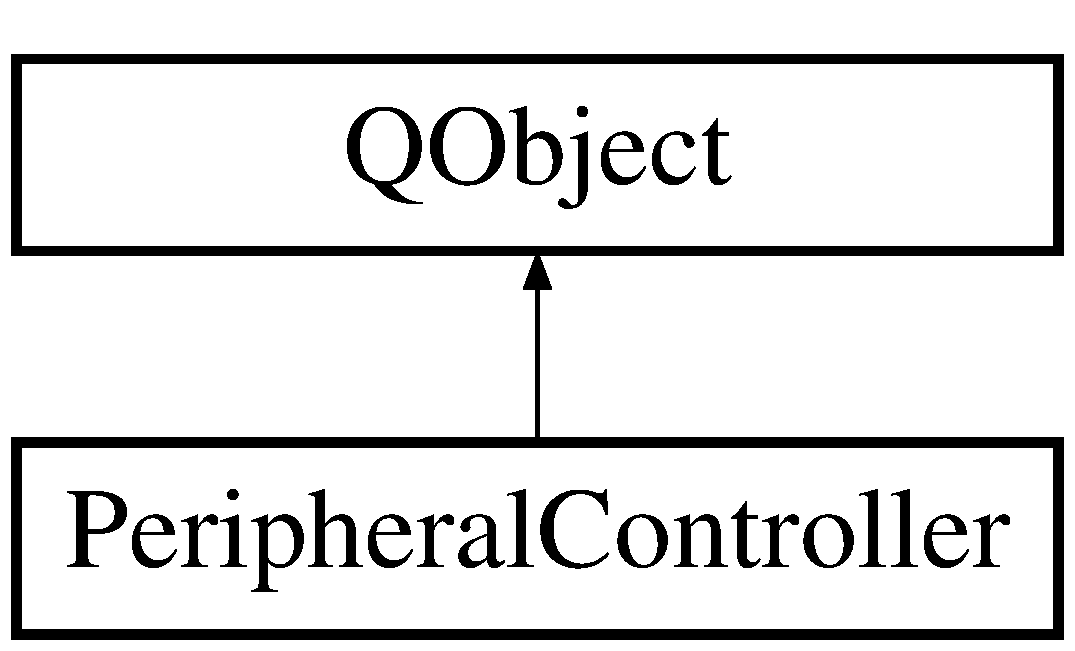
\includegraphics[height=2.000000cm]{da/d45/a00011}
\end{center}
\end{figure}
\subsection*{Public Slots}
\subsection*{Signals}
\subsection*{Public Member Functions}
\subsection*{Static Public Member Functions}
\subsection*{Private Member Functions}
\subsection*{Private Attributes}
\subsection*{Static Private Attributes}


\subsection{Detailed Description}


\subsection{Constructor \& Destructor Documentation}
\hypertarget{a00011_a458a87530aff37dfe6f31899599aea2f}{\index{Peripheral\-Controller@{Peripheral\-Controller}!Peripheral\-Controller@{Peripheral\-Controller}}
\index{Peripheral\-Controller@{Peripheral\-Controller}!PeripheralController@{Peripheral\-Controller}}
\subsubsection[{Peripheral\-Controller}]{\setlength{\rightskip}{0pt plus 5cm}{\bf Peripheral\-Controller} (
\begin{DoxyParamCaption}
{}
\end{DoxyParamCaption}
)\hspace{0.3cm}{\ttfamily [private]}}}\label{a00011_a458a87530aff37dfe6f31899599aea2f}


Constructor. 


\begin{DoxyParams}{Parameters}
{\em none} & \\
\hline
\end{DoxyParams}

\begin{DoxyExceptions}{Exceptions}
{\em none} & \\
\hline
\end{DoxyExceptions}
\begin{DoxyReturn}{Returns}
\hyperlink{a00011}{Peripheral\-Controller} instance 
\end{DoxyReturn}

\begin{DoxyCode}
6 \{
7     \hyperlink{a00011_a2e34a37152be9b74f82195ddd044b40e}{m\_pJoystick} = \textcolor{keyword}{new} \hyperlink{a00005}{JoystickGrabber}();
8 
9     \hyperlink{a00011_a5f850b41f8d146c95fa4fcb5c118ba83}{m\_bMouseMode} = \textcolor{keyword}{true};
10     \hyperlink{a00011_a25f6095115a8ff95c4db48ae47b82211}{m\_bWaitRelease} = \textcolor{keyword}{false};
11     \hyperlink{a00011_aa2bc3dbc15db0a044829d4a20ba08f56}{m\_bWaitReleaseRight} = \textcolor{keyword}{false};
12     \hyperlink{a00011_ad746a6b65e92b161871379fccca76759}{m\_bWaitReleaseMode} = \textcolor{keyword}{false};
13 
14     connect(&\hyperlink{a00011_a8ba25017352f50469eddacb322dea1ea}{m\_pTimer}, SIGNAL(timeout()), \hyperlink{a00011_a2e34a37152be9b74f82195ddd044b40e}{m\_pJoystick}, SLOT(grab()));
15     connect(\hyperlink{a00011_a2e34a37152be9b74f82195ddd044b40e}{m\_pJoystick}, SIGNAL(dataComputed()), \textcolor{keyword}{this}, SLOT(
      \hyperlink{a00011_a4c891561d67bf6739511e3896eba6fb4}{useController}()));
16     connect(\hyperlink{a00011_a2e34a37152be9b74f82195ddd044b40e}{m\_pJoystick}, SIGNAL(dataComputed()), \textcolor{keyword}{this}, SIGNAL(
      \hyperlink{a00011_a35163b56af81dc0f09dc69e92161f4b9}{controllerConnected}()));
17     connect(\hyperlink{a00011_a2e34a37152be9b74f82195ddd044b40e}{m\_pJoystick}, SIGNAL(\hyperlink{a00011_ad70a13ae9071262fc324babf6254d6ea}{noJoystick}()), \textcolor{keyword}{this}, SIGNAL(
      \hyperlink{a00011_ad70a13ae9071262fc324babf6254d6ea}{noJoystick}()));
18     connect(\hyperlink{a00011_a2e34a37152be9b74f82195ddd044b40e}{m\_pJoystick}, SIGNAL(\hyperlink{a00011_a10733eb4d9bf54f33699a23fe0e0c4f8}{directInputProblem}()), \textcolor{keyword}{this}, SIGNAL(
      \hyperlink{a00011_a10733eb4d9bf54f33699a23fe0e0c4f8}{directInputProblem}()));
19     connect(\hyperlink{a00011_a2e34a37152be9b74f82195ddd044b40e}{m\_pJoystick}, SIGNAL(\hyperlink{a00011_aa6bfaa413ce18461ac71e75248460700}{dataFormatProblem}()), \textcolor{keyword}{this}, SIGNAL(
      \hyperlink{a00011_aa6bfaa413ce18461ac71e75248460700}{dataFormatProblem}()));
20     connect(\hyperlink{a00011_a2e34a37152be9b74f82195ddd044b40e}{m\_pJoystick}, SIGNAL(\hyperlink{a00011_a2359b3e182aa100a1c8da8c5d05155fe}{joystickProblem}()), \textcolor{keyword}{this}, SIGNAL(
      \hyperlink{a00011_a2359b3e182aa100a1c8da8c5d05155fe}{joystickProblem}()));
21     connect(\hyperlink{a00011_a2e34a37152be9b74f82195ddd044b40e}{m\_pJoystick}, SIGNAL(\hyperlink{a00011_a51a5a6418d902f49aa198a8d3ae923f6}{deviceEnumProblem}()), \textcolor{keyword}{this}, SIGNAL(
      \hyperlink{a00011_a51a5a6418d902f49aa198a8d3ae923f6}{deviceEnumProblem}()));
22 \}
\end{DoxyCode}
\hypertarget{a00011_a74f9f7dba0d6aee9d6ca60746ff37441}{\index{Peripheral\-Controller@{Peripheral\-Controller}!$\sim$\-Peripheral\-Controller@{$\sim$\-Peripheral\-Controller}}
\index{$\sim$\-Peripheral\-Controller@{$\sim$\-Peripheral\-Controller}!PeripheralController@{Peripheral\-Controller}}
\subsubsection[{$\sim$\-Peripheral\-Controller}]{\setlength{\rightskip}{0pt plus 5cm}$\sim${\bf Peripheral\-Controller} (
\begin{DoxyParamCaption}
{}
\end{DoxyParamCaption}
)\hspace{0.3cm}{\ttfamily [private]}}}\label{a00011_a74f9f7dba0d6aee9d6ca60746ff37441}


Destructor. 


\begin{DoxyParams}{Parameters}
{\em none} & \\
\hline
\end{DoxyParams}

\begin{DoxyExceptions}{Exceptions}
{\em none} & \\
\hline
\end{DoxyExceptions}
\begin{DoxyReturn}{Returns}
none 
\end{DoxyReturn}

\begin{DoxyCode}
44 \{
45 \}
\end{DoxyCode}


\subsection{Member Function Documentation}
\hypertarget{a00011_a35163b56af81dc0f09dc69e92161f4b9}{\index{Peripheral\-Controller@{Peripheral\-Controller}!controller\-Connected@{controller\-Connected}}
\index{controller\-Connected@{controller\-Connected}!PeripheralController@{Peripheral\-Controller}}
\subsubsection[{controller\-Connected}]{\setlength{\rightskip}{0pt plus 5cm}void controller\-Connected (
\begin{DoxyParamCaption}
{}
\end{DoxyParamCaption}
)\hspace{0.3cm}{\ttfamily [signal]}}}\label{a00011_a35163b56af81dc0f09dc69e92161f4b9}


Controller connected event. 


\begin{DoxyParams}{Parameters}
{\em none} & \\
\hline
\end{DoxyParams}

\begin{DoxyExceptions}{Exceptions}
{\em none} & \\
\hline
\end{DoxyExceptions}
\begin{DoxyReturn}{Returns}
none 
\end{DoxyReturn}
\hypertarget{a00011_aff3131ad09d602487d9a2eddf9c10152}{\index{Peripheral\-Controller@{Peripheral\-Controller}!controller\-Control\-Mode@{controller\-Control\-Mode}}
\index{controller\-Control\-Mode@{controller\-Control\-Mode}!PeripheralController@{Peripheral\-Controller}}
\subsubsection[{controller\-Control\-Mode}]{\setlength{\rightskip}{0pt plus 5cm}void controller\-Control\-Mode (
\begin{DoxyParamCaption}
{}
\end{DoxyParamCaption}
)\hspace{0.3cm}{\ttfamily [signal]}}}\label{a00011_aff3131ad09d602487d9a2eddf9c10152}


Controller control mode event. 


\begin{DoxyParams}{Parameters}
{\em none} & \\
\hline
\end{DoxyParams}

\begin{DoxyExceptions}{Exceptions}
{\em none} & \\
\hline
\end{DoxyExceptions}
\begin{DoxyReturn}{Returns}
none 
\end{DoxyReturn}
\hypertarget{a00011_ae805875db5d4bed3c7ae8b42ea448c1f}{\index{Peripheral\-Controller@{Peripheral\-Controller}!controller\-Mouse\-Mode@{controller\-Mouse\-Mode}}
\index{controller\-Mouse\-Mode@{controller\-Mouse\-Mode}!PeripheralController@{Peripheral\-Controller}}
\subsubsection[{controller\-Mouse\-Mode}]{\setlength{\rightskip}{0pt plus 5cm}void controller\-Mouse\-Mode (
\begin{DoxyParamCaption}
{}
\end{DoxyParamCaption}
)\hspace{0.3cm}{\ttfamily [signal]}}}\label{a00011_ae805875db5d4bed3c7ae8b42ea448c1f}


Controller mouse mode event. 


\begin{DoxyParams}{Parameters}
{\em none} & \\
\hline
\end{DoxyParams}

\begin{DoxyExceptions}{Exceptions}
{\em none} & \\
\hline
\end{DoxyExceptions}
\begin{DoxyReturn}{Returns}
none 
\end{DoxyReturn}
\hypertarget{a00011_a2869d5a0199756d4d4f2bcf2889320cf}{\index{Peripheral\-Controller@{Peripheral\-Controller}!control\-Mode@{control\-Mode}}
\index{control\-Mode@{control\-Mode}!PeripheralController@{Peripheral\-Controller}}
\subsubsection[{control\-Mode}]{\setlength{\rightskip}{0pt plus 5cm}void control\-Mode (
\begin{DoxyParamCaption}
{}
\end{DoxyParamCaption}
)\hspace{0.3cm}{\ttfamily [private]}}}\label{a00011_a2869d5a0199756d4d4f2bcf2889320cf}


M\-U\-A\-V control management. 


\begin{DoxyParams}{Parameters}
{\em none} & \\
\hline
\end{DoxyParams}

\begin{DoxyExceptions}{Exceptions}
{\em none} & \\
\hline
\end{DoxyExceptions}
\begin{DoxyReturn}{Returns}
none 
\end{DoxyReturn}

\begin{DoxyCode}
153 \{
154     \textcolor{keywordtype}{double} x = 0, y = 0, z = 0, yaw = 0, height = 0;
155     \textcolor{keywordtype}{bool} bSend = \textcolor{keyword}{false};
156 
157     \textcolor{keywordflow}{if} (\hyperlink{a00011_a2e34a37152be9b74f82195ddd044b40e}{m\_pJoystick}->\hyperlink{a00005_a3db012f463d24f44cefdfef69c495a0e}{leftStickY} < -0.5)
158     \{
159         x = 10;
160         bSend = \textcolor{keyword}{true};
161     \}
162     \textcolor{keywordflow}{else} \textcolor{keywordflow}{if} (\hyperlink{a00011_a2e34a37152be9b74f82195ddd044b40e}{m\_pJoystick}->\hyperlink{a00005_a3db012f463d24f44cefdfef69c495a0e}{leftStickY} > 0.5)
163     \{
164         x = -10;
165         bSend = \textcolor{keyword}{true};
166     \}
167 
168     \textcolor{keywordflow}{if} (\hyperlink{a00011_a2e34a37152be9b74f82195ddd044b40e}{m\_pJoystick}->\hyperlink{a00005_ab182c34f8588348767de30e37ac6c659}{leftStickX} < -0.5)
169     \{
170         y = 10;
171         bSend = \textcolor{keyword}{true};
172     \}
173     \textcolor{keywordflow}{else} \textcolor{keywordflow}{if} (\hyperlink{a00011_a2e34a37152be9b74f82195ddd044b40e}{m\_pJoystick}->\hyperlink{a00005_ab182c34f8588348767de30e37ac6c659}{leftStickX} > 0.5)
174     \{
175         y = -10;
176         bSend = \textcolor{keyword}{true};
177     \}
178 
179     \textcolor{keywordflow}{if} (\hyperlink{a00011_a2e34a37152be9b74f82195ddd044b40e}{m\_pJoystick}->\hyperlink{a00005_af0881450f92ff4ebb21414f6c6f124df}{rightStickX} < -0.5)
180     \{
181         yaw = \hyperlink{a00012_a40277d38c94caf6125045994ba06f18f}{RPA::getInstance}()->\hyperlink{a00012_a8c56441519ab3fa6a971bc898106adc4}{getHeading}() - 10;
182         bSend = \textcolor{keyword}{true};
183 
184         \textcolor{keywordflow}{if} (yaw < 0)
185         \{
186             yaw = \hyperlink{a00012_a40277d38c94caf6125045994ba06f18f}{RPA::getInstance}()->\hyperlink{a00012_a8c56441519ab3fa6a971bc898106adc4}{getHeading}() - 10 + 360;
187         \}
188     \}
189     \textcolor{keywordflow}{else} \textcolor{keywordflow}{if} (\hyperlink{a00011_a2e34a37152be9b74f82195ddd044b40e}{m\_pJoystick}->\hyperlink{a00005_af0881450f92ff4ebb21414f6c6f124df}{rightStickX} > 0.5)
190     \{   
191         yaw = \hyperlink{a00012_a40277d38c94caf6125045994ba06f18f}{RPA::getInstance}()->\hyperlink{a00012_a8c56441519ab3fa6a971bc898106adc4}{getHeading}() + 10;
192         bSend = \textcolor{keyword}{true};
193 
194         \textcolor{keywordflow}{if} (yaw > 360)
195         \{
196             yaw = \hyperlink{a00012_a40277d38c94caf6125045994ba06f18f}{RPA::getInstance}()->\hyperlink{a00012_a8c56441519ab3fa6a971bc898106adc4}{getHeading}() + 10 - 360;
197         \}
198     \}
199 
200     \textcolor{keywordflow}{if} (\hyperlink{a00011_a2e34a37152be9b74f82195ddd044b40e}{m\_pJoystick}->\hyperlink{a00005_a3010a64bd66ee481f2f6c94f368993ef}{topTrigger} < -0.5)
201     \{
202         height = \hyperlink{a00012_a40277d38c94caf6125045994ba06f18f}{RPA::getInstance}()->\hyperlink{a00012_ae1d662c26106ff9692252346d578e8fa}{getHeight}() + 10;
203         bSend = \textcolor{keyword}{true};
204     \}
205     \textcolor{keywordflow}{else} \textcolor{keywordflow}{if} (\hyperlink{a00011_a2e34a37152be9b74f82195ddd044b40e}{m\_pJoystick}->\hyperlink{a00005_a3010a64bd66ee481f2f6c94f368993ef}{topTrigger} > 0.5)
206     \{
207         height = \hyperlink{a00012_a40277d38c94caf6125045994ba06f18f}{RPA::getInstance}()->\hyperlink{a00012_ae1d662c26106ff9692252346d578e8fa}{getHeight}() - 10;
208         bSend = \textcolor{keyword}{true};
209     \}
210 
211     \textcolor{keywordflow}{if} (bSend)
212     \{
213         emit \hyperlink{a00011_a44769de90c2ec83d360149f4b36ea8da}{move}(x, y, height, yaw);
214     \}
215 \}
\end{DoxyCode}
\hypertarget{a00011_aa6bfaa413ce18461ac71e75248460700}{\index{Peripheral\-Controller@{Peripheral\-Controller}!data\-Format\-Problem@{data\-Format\-Problem}}
\index{data\-Format\-Problem@{data\-Format\-Problem}!PeripheralController@{Peripheral\-Controller}}
\subsubsection[{data\-Format\-Problem}]{\setlength{\rightskip}{0pt plus 5cm}void data\-Format\-Problem (
\begin{DoxyParamCaption}
{}
\end{DoxyParamCaption}
)\hspace{0.3cm}{\ttfamily [signal]}}}\label{a00011_aa6bfaa413ce18461ac71e75248460700}


Direct X data format problem. 


\begin{DoxyParams}{Parameters}
{\em none} & \\
\hline
\end{DoxyParams}

\begin{DoxyExceptions}{Exceptions}
{\em none} & \\
\hline
\end{DoxyExceptions}
\begin{DoxyReturn}{Returns}
none 
\end{DoxyReturn}
\hypertarget{a00011_a51a5a6418d902f49aa198a8d3ae923f6}{\index{Peripheral\-Controller@{Peripheral\-Controller}!device\-Enum\-Problem@{device\-Enum\-Problem}}
\index{device\-Enum\-Problem@{device\-Enum\-Problem}!PeripheralController@{Peripheral\-Controller}}
\subsubsection[{device\-Enum\-Problem}]{\setlength{\rightskip}{0pt plus 5cm}void device\-Enum\-Problem (
\begin{DoxyParamCaption}
{}
\end{DoxyParamCaption}
)\hspace{0.3cm}{\ttfamily [signal]}}}\label{a00011_a51a5a6418d902f49aa198a8d3ae923f6}


Device emumeration problem. 


\begin{DoxyParams}{Parameters}
{\em none} & \\
\hline
\end{DoxyParams}

\begin{DoxyExceptions}{Exceptions}
{\em none} & \\
\hline
\end{DoxyExceptions}
\begin{DoxyReturn}{Returns}
none 
\end{DoxyReturn}
\hypertarget{a00011_a10733eb4d9bf54f33699a23fe0e0c4f8}{\index{Peripheral\-Controller@{Peripheral\-Controller}!direct\-Input\-Problem@{direct\-Input\-Problem}}
\index{direct\-Input\-Problem@{direct\-Input\-Problem}!PeripheralController@{Peripheral\-Controller}}
\subsubsection[{direct\-Input\-Problem}]{\setlength{\rightskip}{0pt plus 5cm}void direct\-Input\-Problem (
\begin{DoxyParamCaption}
{}
\end{DoxyParamCaption}
)\hspace{0.3cm}{\ttfamily [signal]}}}\label{a00011_a10733eb4d9bf54f33699a23fe0e0c4f8}


Direct Input problem. 


\begin{DoxyParams}{Parameters}
{\em none} & \\
\hline
\end{DoxyParams}

\begin{DoxyExceptions}{Exceptions}
{\em none} & \\
\hline
\end{DoxyExceptions}
\begin{DoxyReturn}{Returns}
none 
\end{DoxyReturn}
\hypertarget{a00011_a81bd14f0b39bba2433355ec26f833270}{\index{Peripheral\-Controller@{Peripheral\-Controller}!get\-Instance@{get\-Instance}}
\index{get\-Instance@{get\-Instance}!PeripheralController@{Peripheral\-Controller}}
\subsubsection[{get\-Instance}]{\setlength{\rightskip}{0pt plus 5cm}{\bf Peripheral\-Controller} $\ast$ get\-Instance (
\begin{DoxyParamCaption}
{}
\end{DoxyParamCaption}
)\hspace{0.3cm}{\ttfamily [static]}}}\label{a00011_a81bd14f0b39bba2433355ec26f833270}


Get the lone instance. 


\begin{DoxyParams}{Parameters}
{\em none} & \\
\hline
\end{DoxyParams}

\begin{DoxyExceptions}{Exceptions}
{\em none} & \\
\hline
\end{DoxyExceptions}
\begin{DoxyReturn}{Returns}
\hyperlink{a00011}{Peripheral\-Controller} instance Peripheral\-Controller$\ast$ 
\end{DoxyReturn}

\begin{DoxyCode}
25 \{
26     \textcolor{keywordflow}{if} (\hyperlink{a00011_a4c732b19b7b708ba880e1a7dd193d4b2}{singleton} == NULL)
27     \{
28         \hyperlink{a00011_a4c732b19b7b708ba880e1a7dd193d4b2}{singleton} = \textcolor{keyword}{new} \hyperlink{a00011_a458a87530aff37dfe6f31899599aea2f}{PeripheralController}();
29     \}
30 
31     \textcolor{keywordflow}{return} \hyperlink{a00011_a4c732b19b7b708ba880e1a7dd193d4b2}{singleton};
32 \}
\end{DoxyCode}
\hypertarget{a00011_adf02fcb4d0f62c09a87788789f30a0f4}{\index{Peripheral\-Controller@{Peripheral\-Controller}!is\-Mouse\-Mode@{is\-Mouse\-Mode}}
\index{is\-Mouse\-Mode@{is\-Mouse\-Mode}!PeripheralController@{Peripheral\-Controller}}
\subsubsection[{is\-Mouse\-Mode}]{\setlength{\rightskip}{0pt plus 5cm}bool is\-Mouse\-Mode (
\begin{DoxyParamCaption}
{}
\end{DoxyParamCaption}
)}}\label{a00011_adf02fcb4d0f62c09a87788789f30a0f4}


Mouse mode activated indicator. 


\begin{DoxyParams}{Parameters}
{\em none} & \\
\hline
\end{DoxyParams}

\begin{DoxyExceptions}{Exceptions}
{\em none} & \\
\hline
\end{DoxyExceptions}
\begin{DoxyReturn}{Returns}
In mouse mode bool 
\end{DoxyReturn}

\begin{DoxyCode}
218 \{
219     \textcolor{keywordflow}{return} \hyperlink{a00011_a5f850b41f8d146c95fa4fcb5c118ba83}{m\_bMouseMode};
220 \}
\end{DoxyCode}
\hypertarget{a00011_a2359b3e182aa100a1c8da8c5d05155fe}{\index{Peripheral\-Controller@{Peripheral\-Controller}!joystick\-Problem@{joystick\-Problem}}
\index{joystick\-Problem@{joystick\-Problem}!PeripheralController@{Peripheral\-Controller}}
\subsubsection[{joystick\-Problem}]{\setlength{\rightskip}{0pt plus 5cm}void joystick\-Problem (
\begin{DoxyParamCaption}
{}
\end{DoxyParamCaption}
)\hspace{0.3cm}{\ttfamily [signal]}}}\label{a00011_a2359b3e182aa100a1c8da8c5d05155fe}


Game controller device state get problem. 


\begin{DoxyParams}{Parameters}
{\em none} & \\
\hline
\end{DoxyParams}

\begin{DoxyExceptions}{Exceptions}
{\em none} & \\
\hline
\end{DoxyExceptions}
\begin{DoxyReturn}{Returns}
none 
\end{DoxyReturn}
\hypertarget{a00011_aae9d52caad9fb2892deeb25596cfd2ab}{\index{Peripheral\-Controller@{Peripheral\-Controller}!kill@{kill}}
\index{kill@{kill}!PeripheralController@{Peripheral\-Controller}}
\subsubsection[{kill}]{\setlength{\rightskip}{0pt plus 5cm}void kill (
\begin{DoxyParamCaption}
{}
\end{DoxyParamCaption}
)\hspace{0.3cm}{\ttfamily [static]}}}\label{a00011_aae9d52caad9fb2892deeb25596cfd2ab}


Lone instance killer. 


\begin{DoxyParams}{Parameters}
{\em none} & \\
\hline
\end{DoxyParams}

\begin{DoxyExceptions}{Exceptions}
{\em none} & \\
\hline
\end{DoxyExceptions}
\begin{DoxyReturn}{Returns}
none 
\end{DoxyReturn}

\begin{DoxyCode}
35 \{
36     \textcolor{keywordflow}{if} (\hyperlink{a00011_a4c732b19b7b708ba880e1a7dd193d4b2}{singleton} != NULL)
37     \{
38         \textcolor{keyword}{delete} \hyperlink{a00011_a4c732b19b7b708ba880e1a7dd193d4b2}{singleton};
39         \hyperlink{a00011_a4c732b19b7b708ba880e1a7dd193d4b2}{singleton} = NULL;
40     \}
41 \}
\end{DoxyCode}
\hypertarget{a00011_aa90a20f7c02554ca9335896cbc476ffc}{\index{Peripheral\-Controller@{Peripheral\-Controller}!mouse\-Event@{mouse\-Event}}
\index{mouse\-Event@{mouse\-Event}!PeripheralController@{Peripheral\-Controller}}
\subsubsection[{mouse\-Event}]{\setlength{\rightskip}{0pt plus 5cm}void mouse\-Event (
\begin{DoxyParamCaption}
\item[{Qt\-::\-Mouse\-Button}]{button, }
\item[{bool}]{wait\-Release}
\end{DoxyParamCaption}
)\hspace{0.3cm}{\ttfamily [signal]}}}\label{a00011_aa90a20f7c02554ca9335896cbc476ffc}


Mouse event reagrding actions on gamepad. 


\begin{DoxyParams}{Parameters}
{\em button} & emulated pressed button Qt\-::\-Mouse\-Button \\
\hline
{\em wait\-Release} & button already pressed bool \\
\hline
\end{DoxyParams}

\begin{DoxyExceptions}{Exceptions}
{\em none} & \\
\hline
\end{DoxyExceptions}
\begin{DoxyReturn}{Returns}
none 
\end{DoxyReturn}
\hypertarget{a00011_a80b77ca519ad5f2104e456dc862f431a}{\index{Peripheral\-Controller@{Peripheral\-Controller}!mouse\-Mode@{mouse\-Mode}}
\index{mouse\-Mode@{mouse\-Mode}!PeripheralController@{Peripheral\-Controller}}
\subsubsection[{mouse\-Mode}]{\setlength{\rightskip}{0pt plus 5cm}void mouse\-Mode (
\begin{DoxyParamCaption}
{}
\end{DoxyParamCaption}
)\hspace{0.3cm}{\ttfamily [private]}}}\label{a00011_a80b77ca519ad5f2104e456dc862f431a}


Mouse mode management. 


\begin{DoxyParams}{Parameters}
{\em none} & \\
\hline
\end{DoxyParams}

\begin{DoxyExceptions}{Exceptions}
{\em none} & \\
\hline
\end{DoxyExceptions}
\begin{DoxyReturn}{Returns}
none 
\end{DoxyReturn}

\begin{DoxyCode}
84 \{
85     \textcolor{keywordtype}{bool} modified = \textcolor{keyword}{false};
86     \textcolor{keywordtype}{int} x, y;
87     QPoint position = QCursor::pos();
88 
89     x = position.x();
90     y = position.y();
91 
92     \textcolor{keywordflow}{if} (\hyperlink{a00011_a2e34a37152be9b74f82195ddd044b40e}{m\_pJoystick}->\hyperlink{a00005_ab182c34f8588348767de30e37ac6c659}{leftStickX} < -0.7 || \hyperlink{a00011_a2e34a37152be9b74f82195ddd044b40e}{m\_pJoystick}->
      \hyperlink{a00005_ab182c34f8588348767de30e37ac6c659}{leftStickX} > 0.7)
93     \{
94         modified = \textcolor{keyword}{true};
95         x = position.x() + (int)(\hyperlink{a00011_a2e34a37152be9b74f82195ddd044b40e}{m\_pJoystick}->\hyperlink{a00005_ab182c34f8588348767de30e37ac6c659}{leftStickX} * 50);
96     \}
97     \textcolor{keywordflow}{else} \textcolor{keywordflow}{if} (\hyperlink{a00011_a2e34a37152be9b74f82195ddd044b40e}{m\_pJoystick}->\hyperlink{a00005_ab182c34f8588348767de30e37ac6c659}{leftStickX} < -0.4 || \hyperlink{a00011_a2e34a37152be9b74f82195ddd044b40e}{m\_pJoystick}->
      \hyperlink{a00005_ab182c34f8588348767de30e37ac6c659}{leftStickX} > 0.4)
98     \{
99         modified = \textcolor{keyword}{true};
100         x = position.x() + (int)(\hyperlink{a00011_a2e34a37152be9b74f82195ddd044b40e}{m\_pJoystick}->\hyperlink{a00005_ab182c34f8588348767de30e37ac6c659}{leftStickX} * 20);
101     \}
102     \textcolor{keywordflow}{else} \textcolor{keywordflow}{if} (\hyperlink{a00011_a2e34a37152be9b74f82195ddd044b40e}{m\_pJoystick}->\hyperlink{a00005_ab182c34f8588348767de30e37ac6c659}{leftStickX} < -0.2 || \hyperlink{a00011_a2e34a37152be9b74f82195ddd044b40e}{m\_pJoystick}->
      \hyperlink{a00005_ab182c34f8588348767de30e37ac6c659}{leftStickX} > 0.2)
103     \{
104         modified = \textcolor{keyword}{true};
105         x = position.x() + (int)(\hyperlink{a00011_a2e34a37152be9b74f82195ddd044b40e}{m\_pJoystick}->\hyperlink{a00005_ab182c34f8588348767de30e37ac6c659}{leftStickX} * 10);
106     \}
107 
108     \textcolor{keywordflow}{if} (\hyperlink{a00011_a2e34a37152be9b74f82195ddd044b40e}{m\_pJoystick}->\hyperlink{a00005_a3db012f463d24f44cefdfef69c495a0e}{leftStickY} < -0.7 || \hyperlink{a00011_a2e34a37152be9b74f82195ddd044b40e}{m\_pJoystick}->
      \hyperlink{a00005_a3db012f463d24f44cefdfef69c495a0e}{leftStickY} > 0.7)
109     \{
110         modified = \textcolor{keyword}{true};
111         y = position.y() + (int)(\hyperlink{a00011_a2e34a37152be9b74f82195ddd044b40e}{m\_pJoystick}->\hyperlink{a00005_a3db012f463d24f44cefdfef69c495a0e}{leftStickY} * 50);
112     \}
113     \textcolor{keywordflow}{else} \textcolor{keywordflow}{if} (\hyperlink{a00011_a2e34a37152be9b74f82195ddd044b40e}{m\_pJoystick}->\hyperlink{a00005_a3db012f463d24f44cefdfef69c495a0e}{leftStickY} < -0.4 || \hyperlink{a00011_a2e34a37152be9b74f82195ddd044b40e}{m\_pJoystick}->
      \hyperlink{a00005_a3db012f463d24f44cefdfef69c495a0e}{leftStickY} > 0.4)
114     \{
115         modified = \textcolor{keyword}{true};
116         y = position.y() + (int)(\hyperlink{a00011_a2e34a37152be9b74f82195ddd044b40e}{m\_pJoystick}->\hyperlink{a00005_a3db012f463d24f44cefdfef69c495a0e}{leftStickY} * 20);
117     \}
118     \textcolor{keywordflow}{else} \textcolor{keywordflow}{if} (\hyperlink{a00011_a2e34a37152be9b74f82195ddd044b40e}{m\_pJoystick}->\hyperlink{a00005_a3db012f463d24f44cefdfef69c495a0e}{leftStickY} < -0.2 || \hyperlink{a00011_a2e34a37152be9b74f82195ddd044b40e}{m\_pJoystick}->
      \hyperlink{a00005_a3db012f463d24f44cefdfef69c495a0e}{leftStickY} > 0.2)
119     \{
120         modified = \textcolor{keyword}{true};
121         y = position.y() + (int)(\hyperlink{a00011_a2e34a37152be9b74f82195ddd044b40e}{m\_pJoystick}->\hyperlink{a00005_a3db012f463d24f44cefdfef69c495a0e}{leftStickY} * 10);
122     \}
123 
124     \textcolor{keywordflow}{if} (\hyperlink{a00011_a2e34a37152be9b74f82195ddd044b40e}{m\_pJoystick}->\hyperlink{a00005_a79f4acbf0893aed36f0bf600410b9fde}{buttons}[0] == \textcolor{keyword}{true} && !\hyperlink{a00011_a25f6095115a8ff95c4db48ae47b82211}{m\_bWaitRelease})
125     \{ 
126         emit \hyperlink{a00011_aa90a20f7c02554ca9335896cbc476ffc}{mouseEvent}(Qt::LeftButton, \hyperlink{a00011_a25f6095115a8ff95c4db48ae47b82211}{m\_bWaitRelease});
127         \hyperlink{a00011_a25f6095115a8ff95c4db48ae47b82211}{m\_bWaitRelease} = \textcolor{keyword}{true};
128     \}
129     \textcolor{keywordflow}{else} \textcolor{keywordflow}{if} (\hyperlink{a00011_a2e34a37152be9b74f82195ddd044b40e}{m\_pJoystick}->\hyperlink{a00005_a79f4acbf0893aed36f0bf600410b9fde}{buttons}[0] == \textcolor{keyword}{false} && 
      \hyperlink{a00011_a25f6095115a8ff95c4db48ae47b82211}{m\_bWaitRelease} == \textcolor{keyword}{true})
130     \{
131         emit \hyperlink{a00011_aa90a20f7c02554ca9335896cbc476ffc}{mouseEvent}(Qt::LeftButton, \hyperlink{a00011_a25f6095115a8ff95c4db48ae47b82211}{m\_bWaitRelease});
132         \hyperlink{a00011_a25f6095115a8ff95c4db48ae47b82211}{m\_bWaitRelease} = \textcolor{keyword}{false};
133     \}
134 
135     \textcolor{keywordflow}{if} (\hyperlink{a00011_a2e34a37152be9b74f82195ddd044b40e}{m\_pJoystick}->\hyperlink{a00005_a79f4acbf0893aed36f0bf600410b9fde}{buttons}[1] == \textcolor{keyword}{true} && !
      \hyperlink{a00011_aa2bc3dbc15db0a044829d4a20ba08f56}{m\_bWaitReleaseRight})
136     \{ 
137         emit \hyperlink{a00011_aa90a20f7c02554ca9335896cbc476ffc}{mouseEvent}(Qt::RightButton, \hyperlink{a00011_aa2bc3dbc15db0a044829d4a20ba08f56}{m\_bWaitReleaseRight});
138         \hyperlink{a00011_aa2bc3dbc15db0a044829d4a20ba08f56}{m\_bWaitReleaseRight} = \textcolor{keyword}{true};
139     \}
140     \textcolor{keywordflow}{else} \textcolor{keywordflow}{if} (\hyperlink{a00011_a2e34a37152be9b74f82195ddd044b40e}{m\_pJoystick}->\hyperlink{a00005_a79f4acbf0893aed36f0bf600410b9fde}{buttons}[1] == \textcolor{keyword}{false} && 
      \hyperlink{a00011_aa2bc3dbc15db0a044829d4a20ba08f56}{m\_bWaitReleaseRight} == \textcolor{keyword}{true})
141     \{
142         emit \hyperlink{a00011_aa90a20f7c02554ca9335896cbc476ffc}{mouseEvent}(Qt::RightButton, \hyperlink{a00011_aa2bc3dbc15db0a044829d4a20ba08f56}{m\_bWaitReleaseRight});
143         \hyperlink{a00011_aa2bc3dbc15db0a044829d4a20ba08f56}{m\_bWaitReleaseRight} = \textcolor{keyword}{false};
144     \}
145 
146     \textcolor{keywordflow}{if} (modified)
147     \{
148         QCursor::setPos(x, y);
149     \}
150 \}
\end{DoxyCode}
\hypertarget{a00011_a44769de90c2ec83d360149f4b36ea8da}{\index{Peripheral\-Controller@{Peripheral\-Controller}!move@{move}}
\index{move@{move}!PeripheralController@{Peripheral\-Controller}}
\subsubsection[{move}]{\setlength{\rightskip}{0pt plus 5cm}void move (
\begin{DoxyParamCaption}
\item[{double}]{x, }
\item[{double}]{y, }
\item[{double}]{z, }
\item[{double}]{yaw}
\end{DoxyParamCaption}
)\hspace{0.3cm}{\ttfamily [signal]}}}\label{a00011_a44769de90c2ec83d360149f4b36ea8da}


\hyperlink{a00017}{Waypoint} to send. 


\begin{DoxyParams}{Parameters}
{\em x} & in meters double \\
\hline
{\em y} & in meters double \\
\hline
{\em z} & altitude double \\
\hline
{\em yaw} & heading double \\
\hline
\end{DoxyParams}

\begin{DoxyExceptions}{Exceptions}
{\em none} & \\
\hline
\end{DoxyExceptions}
\begin{DoxyReturn}{Returns}
none 
\end{DoxyReturn}
\hypertarget{a00011_ad70a13ae9071262fc324babf6254d6ea}{\index{Peripheral\-Controller@{Peripheral\-Controller}!no\-Joystick@{no\-Joystick}}
\index{no\-Joystick@{no\-Joystick}!PeripheralController@{Peripheral\-Controller}}
\subsubsection[{no\-Joystick}]{\setlength{\rightskip}{0pt plus 5cm}void no\-Joystick (
\begin{DoxyParamCaption}
{}
\end{DoxyParamCaption}
)\hspace{0.3cm}{\ttfamily [signal]}}}\label{a00011_ad70a13ae9071262fc324babf6254d6ea}


No joystick event. 


\begin{DoxyParams}{Parameters}
{\em none} & \\
\hline
\end{DoxyParams}

\begin{DoxyExceptions}{Exceptions}
{\em none} & \\
\hline
\end{DoxyExceptions}
\begin{DoxyReturn}{Returns}
none 
\end{DoxyReturn}
\hypertarget{a00011_a8928745e5087fc002cf95365e70eec25}{\index{Peripheral\-Controller@{Peripheral\-Controller}!start\-Controller\-Grab@{start\-Controller\-Grab}}
\index{start\-Controller\-Grab@{start\-Controller\-Grab}!PeripheralController@{Peripheral\-Controller}}
\subsubsection[{start\-Controller\-Grab}]{\setlength{\rightskip}{0pt plus 5cm}void start\-Controller\-Grab (
\begin{DoxyParamCaption}
\item[{int}]{p\-\_\-n\-Time}
\end{DoxyParamCaption}
)}}\label{a00011_a8928745e5087fc002cf95365e70eec25}


Start grab timer. 


\begin{DoxyParams}{Parameters}
{\em p\-\_\-n\-Time} & interval time in ms for grab int \\
\hline
\end{DoxyParams}

\begin{DoxyExceptions}{Exceptions}
{\em none} & \\
\hline
\end{DoxyExceptions}
\begin{DoxyReturn}{Returns}
none 
\end{DoxyReturn}

\begin{DoxyCode}
48 \{
49     \hyperlink{a00011_a8ba25017352f50469eddacb322dea1ea}{m\_pTimer}.start(p\_nTime);
50 \}
\end{DoxyCode}
\hypertarget{a00011_a4c891561d67bf6739511e3896eba6fb4}{\index{Peripheral\-Controller@{Peripheral\-Controller}!use\-Controller@{use\-Controller}}
\index{use\-Controller@{use\-Controller}!PeripheralController@{Peripheral\-Controller}}
\subsubsection[{use\-Controller}]{\setlength{\rightskip}{0pt plus 5cm}void use\-Controller (
\begin{DoxyParamCaption}
{}
\end{DoxyParamCaption}
)\hspace{0.3cm}{\ttfamily [slot]}}}\label{a00011_a4c891561d67bf6739511e3896eba6fb4}


Controller handle slot (timed by another software controller) 


\begin{DoxyParams}{Parameters}
{\em none} & \\
\hline
\end{DoxyParams}

\begin{DoxyExceptions}{Exceptions}
{\em none} & \\
\hline
\end{DoxyExceptions}
\begin{DoxyReturn}{Returns}
none 
\end{DoxyReturn}

\begin{DoxyCode}
53 \{
54     \textcolor{keywordflow}{if} (\hyperlink{a00011_a2e34a37152be9b74f82195ddd044b40e}{m\_pJoystick}->\hyperlink{a00005_a79f4acbf0893aed36f0bf600410b9fde}{buttons}[5] == \textcolor{keyword}{true} && !\hyperlink{a00011_ad746a6b65e92b161871379fccca76759}{m\_bWaitReleaseMode})
55     \{
56         \hyperlink{a00011_ad746a6b65e92b161871379fccca76759}{m\_bWaitReleaseMode} = \textcolor{keyword}{true};
57         \hyperlink{a00011_a5f850b41f8d146c95fa4fcb5c118ba83}{m\_bMouseMode} = !\hyperlink{a00011_a5f850b41f8d146c95fa4fcb5c118ba83}{m\_bMouseMode};
58 
59         \textcolor{keywordflow}{if} (\hyperlink{a00011_a5f850b41f8d146c95fa4fcb5c118ba83}{m\_bMouseMode})
60         \{
61             emit \hyperlink{a00011_ae805875db5d4bed3c7ae8b42ea448c1f}{controllerMouseMode}();
62         \}
63         \textcolor{keywordflow}{else}
64         \{
65             emit \hyperlink{a00011_aff3131ad09d602487d9a2eddf9c10152}{controllerControlMode}();
66         \}
67     \}
68     \textcolor{keywordflow}{else} \textcolor{keywordflow}{if} (\hyperlink{a00011_a2e34a37152be9b74f82195ddd044b40e}{m\_pJoystick}->\hyperlink{a00005_a79f4acbf0893aed36f0bf600410b9fde}{buttons}[5] == \textcolor{keyword}{false} && 
      \hyperlink{a00011_ad746a6b65e92b161871379fccca76759}{m\_bWaitReleaseMode})
69     \{
70         \hyperlink{a00011_ad746a6b65e92b161871379fccca76759}{m\_bWaitReleaseMode} = \textcolor{keyword}{false};
71     \}
72 
73     \textcolor{keywordflow}{if} (\hyperlink{a00011_a5f850b41f8d146c95fa4fcb5c118ba83}{m\_bMouseMode})
74     \{
75         \hyperlink{a00011_a80b77ca519ad5f2104e456dc862f431a}{mouseMode}();
76     \}
77     \textcolor{keywordflow}{else}
78     \{
79         \hyperlink{a00011_a2869d5a0199756d4d4f2bcf2889320cf}{controlMode}();
80     \}
81 \}
\end{DoxyCode}


\subsection{Field Documentation}
\hypertarget{a00011_a5f850b41f8d146c95fa4fcb5c118ba83}{\index{Peripheral\-Controller@{Peripheral\-Controller}!m\-\_\-b\-Mouse\-Mode@{m\-\_\-b\-Mouse\-Mode}}
\index{m\-\_\-b\-Mouse\-Mode@{m\-\_\-b\-Mouse\-Mode}!PeripheralController@{Peripheral\-Controller}}
\subsubsection[{m\-\_\-b\-Mouse\-Mode}]{\setlength{\rightskip}{0pt plus 5cm}bool m\-\_\-b\-Mouse\-Mode\hspace{0.3cm}{\ttfamily [private]}}}\label{a00011_a5f850b41f8d146c95fa4fcb5c118ba83}
\hypertarget{a00011_a25f6095115a8ff95c4db48ae47b82211}{\index{Peripheral\-Controller@{Peripheral\-Controller}!m\-\_\-b\-Wait\-Release@{m\-\_\-b\-Wait\-Release}}
\index{m\-\_\-b\-Wait\-Release@{m\-\_\-b\-Wait\-Release}!PeripheralController@{Peripheral\-Controller}}
\subsubsection[{m\-\_\-b\-Wait\-Release}]{\setlength{\rightskip}{0pt plus 5cm}bool m\-\_\-b\-Wait\-Release\hspace{0.3cm}{\ttfamily [private]}}}\label{a00011_a25f6095115a8ff95c4db48ae47b82211}
\hypertarget{a00011_ad746a6b65e92b161871379fccca76759}{\index{Peripheral\-Controller@{Peripheral\-Controller}!m\-\_\-b\-Wait\-Release\-Mode@{m\-\_\-b\-Wait\-Release\-Mode}}
\index{m\-\_\-b\-Wait\-Release\-Mode@{m\-\_\-b\-Wait\-Release\-Mode}!PeripheralController@{Peripheral\-Controller}}
\subsubsection[{m\-\_\-b\-Wait\-Release\-Mode}]{\setlength{\rightskip}{0pt plus 5cm}bool m\-\_\-b\-Wait\-Release\-Mode\hspace{0.3cm}{\ttfamily [private]}}}\label{a00011_ad746a6b65e92b161871379fccca76759}
\hypertarget{a00011_aa2bc3dbc15db0a044829d4a20ba08f56}{\index{Peripheral\-Controller@{Peripheral\-Controller}!m\-\_\-b\-Wait\-Release\-Right@{m\-\_\-b\-Wait\-Release\-Right}}
\index{m\-\_\-b\-Wait\-Release\-Right@{m\-\_\-b\-Wait\-Release\-Right}!PeripheralController@{Peripheral\-Controller}}
\subsubsection[{m\-\_\-b\-Wait\-Release\-Right}]{\setlength{\rightskip}{0pt plus 5cm}bool m\-\_\-b\-Wait\-Release\-Right\hspace{0.3cm}{\ttfamily [private]}}}\label{a00011_aa2bc3dbc15db0a044829d4a20ba08f56}
\hypertarget{a00011_a2e34a37152be9b74f82195ddd044b40e}{\index{Peripheral\-Controller@{Peripheral\-Controller}!m\-\_\-p\-Joystick@{m\-\_\-p\-Joystick}}
\index{m\-\_\-p\-Joystick@{m\-\_\-p\-Joystick}!PeripheralController@{Peripheral\-Controller}}
\subsubsection[{m\-\_\-p\-Joystick}]{\setlength{\rightskip}{0pt plus 5cm}{\bf Joystick\-Grabber}$\ast$ m\-\_\-p\-Joystick\hspace{0.3cm}{\ttfamily [private]}}}\label{a00011_a2e34a37152be9b74f82195ddd044b40e}
\hypertarget{a00011_a8ba25017352f50469eddacb322dea1ea}{\index{Peripheral\-Controller@{Peripheral\-Controller}!m\-\_\-p\-Timer@{m\-\_\-p\-Timer}}
\index{m\-\_\-p\-Timer@{m\-\_\-p\-Timer}!PeripheralController@{Peripheral\-Controller}}
\subsubsection[{m\-\_\-p\-Timer}]{\setlength{\rightskip}{0pt plus 5cm}Q\-Timer m\-\_\-p\-Timer\hspace{0.3cm}{\ttfamily [private]}}}\label{a00011_a8ba25017352f50469eddacb322dea1ea}
\hypertarget{a00011_aeda9d6618a0c455de69329344070cfe4}{\index{Peripheral\-Controller@{Peripheral\-Controller}!problem\-Detected@{problem\-Detected}}
\index{problem\-Detected@{problem\-Detected}!PeripheralController@{Peripheral\-Controller}}
\subsubsection[{problem\-Detected}]{\setlength{\rightskip}{0pt plus 5cm}bool problem\-Detected\hspace{0.3cm}{\ttfamily [private]}}}\label{a00011_aeda9d6618a0c455de69329344070cfe4}
\hypertarget{a00011_a4c732b19b7b708ba880e1a7dd193d4b2}{\index{Peripheral\-Controller@{Peripheral\-Controller}!singleton@{singleton}}
\index{singleton@{singleton}!PeripheralController@{Peripheral\-Controller}}
\subsubsection[{singleton}]{\setlength{\rightskip}{0pt plus 5cm}{\bf Peripheral\-Controller} $\ast$ singleton = N\-U\-L\-L\hspace{0.3cm}{\ttfamily [static]}, {\ttfamily [private]}}}\label{a00011_a4c732b19b7b708ba880e1a7dd193d4b2}


The documentation for this class was generated from the following files\-:\begin{DoxyCompactItemize}
\item 
\hyperlink{a00035}{Peripheral\-Controller.\-h}\item 
\hyperlink{a00034}{Peripheral\-Controller.\-cpp}\end{DoxyCompactItemize}

\hypertarget{a00012}{\section{R\-P\-A Class Reference}
\label{a00012}\index{R\-P\-A@{R\-P\-A}}
}


{\ttfamily \#include \char`\"{}R\-P\-A.\-h\char`\"{}}

Inheritance diagram for R\-P\-A\-:\begin{figure}[H]
\begin{center}
\leavevmode
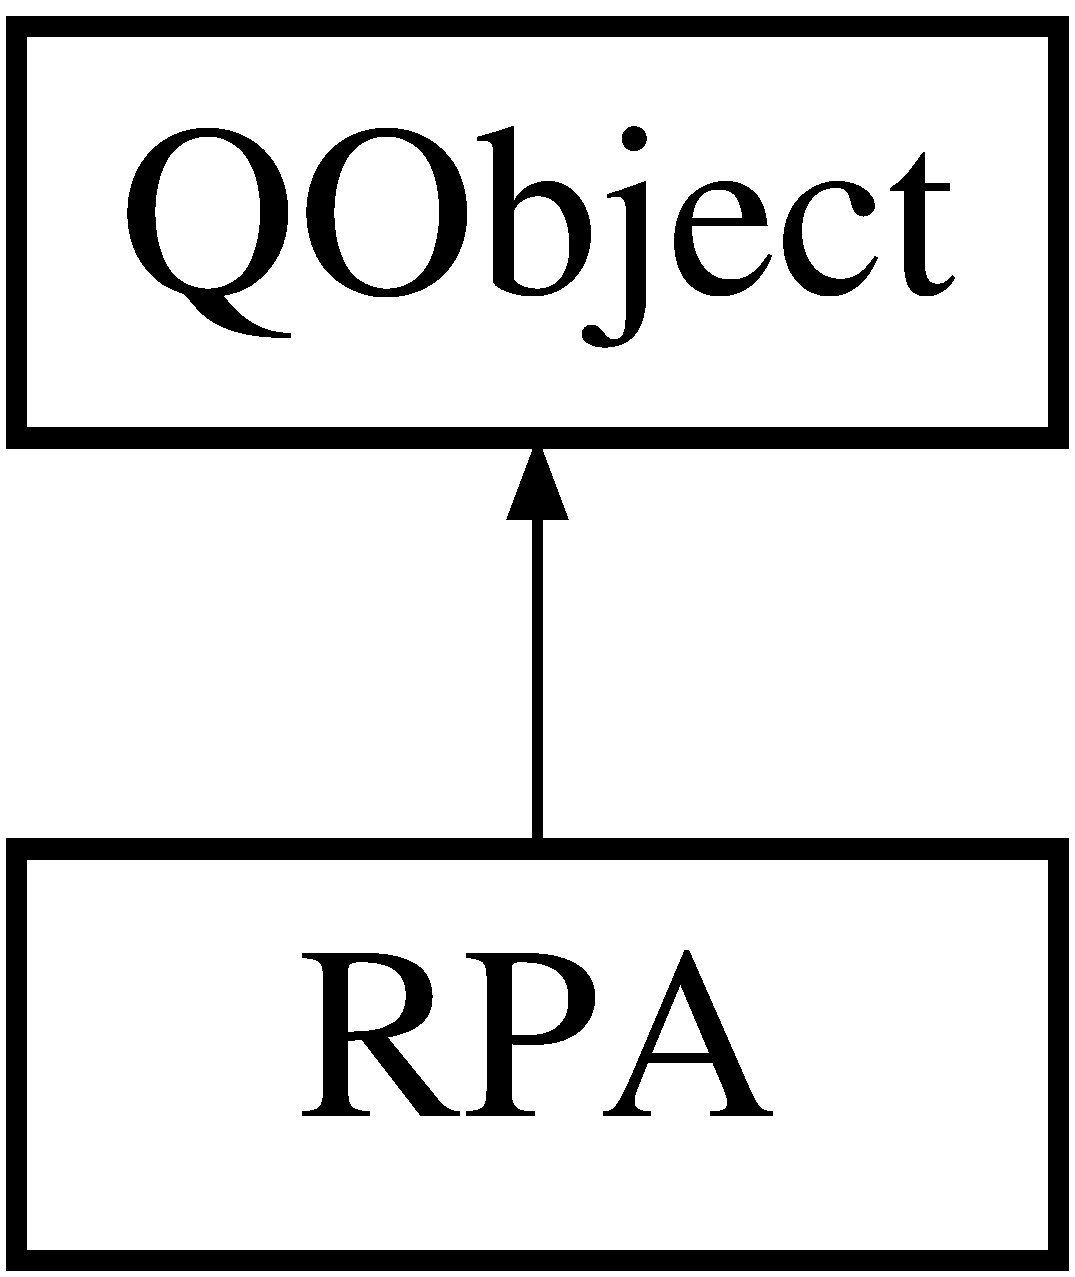
\includegraphics[height=2.000000cm]{df/d86/a00012}
\end{center}
\end{figure}
\subsection*{Public Slots}
\subsection*{Signals}
\subsection*{Public Member Functions}
\subsection*{Static Public Member Functions}
\subsection*{Private Member Functions}
\subsection*{Private Attributes}
\subsection*{Static Private Attributes}


\subsection{Detailed Description}


\subsection{Constructor \& Destructor Documentation}
\hypertarget{a00012_abe9ae8f14b57b3de791786e7c0852b1a}{\index{R\-P\-A@{R\-P\-A}!R\-P\-A@{R\-P\-A}}
\index{R\-P\-A@{R\-P\-A}!RPA@{R\-P\-A}}
\subsubsection[{R\-P\-A}]{\setlength{\rightskip}{0pt plus 5cm}{\bf R\-P\-A} (
\begin{DoxyParamCaption}
{}
\end{DoxyParamCaption}
)\hspace{0.3cm}{\ttfamily [private]}}}\label{a00012_abe9ae8f14b57b3de791786e7c0852b1a}


Constructor. 


\begin{DoxyParams}{Parameters}
{\em none} & \\
\hline
\end{DoxyParams}

\begin{DoxyExceptions}{Exceptions}
{\em none} & \\
\hline
\end{DoxyExceptions}
\begin{DoxyReturn}{Returns}
\hyperlink{a00012}{R\-P\-A} instance 
\end{DoxyReturn}

\begin{DoxyCode}
6 \{
7     \hyperlink{a00012_a0af541d1b4b8c59e4385c003e377b746}{m\_pPosition} = \textcolor{keyword}{new} \hyperlink{a00006}{LatLongCoord}();
8     \hyperlink{a00012_a79a2bd07a373f3b0042e6c2dc0e51fc0}{m\_dAltitude} = 0;
9     \hyperlink{a00012_a610bb35047703e6c2c0176285cd09312}{m\_dHeading} = 0;
10 
11     connect(\hyperlink{a00007_adb2b1b18fad4caaafde371f991525f38}{LogReplayControl::getInstance}(), SIGNAL(
      \hyperlink{a00012_a04e801b333f118c8877267b1797cfe24}{geolocation}(\textcolor{keywordtype}{double}, \textcolor{keywordtype}{double}, \textcolor{keywordtype}{double}, \textcolor{keywordtype}{double})), 
12         \textcolor{keyword}{this}, SLOT(\hyperlink{a00012_a04e801b333f118c8877267b1797cfe24}{geolocation}(\textcolor{keywordtype}{double}, \textcolor{keywordtype}{double}, \textcolor{keywordtype}{double}, \textcolor{keywordtype}{double})));
13     connect(\hyperlink{a00007_adb2b1b18fad4caaafde371f991525f38}{LogReplayControl::getInstance}(), SIGNAL(
      \hyperlink{a00012_aa3c54f0958638486df2b69a9b53c5d7f}{updateHeading}(\textcolor{keywordtype}{double})), \textcolor{keyword}{this}, SLOT(\hyperlink{a00012_aa3c54f0958638486df2b69a9b53c5d7f}{updateHeading}(\textcolor{keywordtype}{double})));
14 \}
\end{DoxyCode}
\hypertarget{a00012_a4043fd156cb502931774dc35bc00fdde}{\index{R\-P\-A@{R\-P\-A}!$\sim$\-R\-P\-A@{$\sim$\-R\-P\-A}}
\index{$\sim$\-R\-P\-A@{$\sim$\-R\-P\-A}!RPA@{R\-P\-A}}
\subsubsection[{$\sim$\-R\-P\-A}]{\setlength{\rightskip}{0pt plus 5cm}$\sim${\bf R\-P\-A} (
\begin{DoxyParamCaption}
{}
\end{DoxyParamCaption}
)\hspace{0.3cm}{\ttfamily [private]}}}\label{a00012_a4043fd156cb502931774dc35bc00fdde}


Destructor. 


\begin{DoxyParams}{Parameters}
{\em none} & \\
\hline
\end{DoxyParams}

\begin{DoxyExceptions}{Exceptions}
{\em none} & \\
\hline
\end{DoxyExceptions}
\begin{DoxyReturn}{Returns}
none 
\end{DoxyReturn}

\begin{DoxyCode}
26 \{
27     \textcolor{keyword}{delete} \hyperlink{a00012_a0af541d1b4b8c59e4385c003e377b746}{m\_pPosition};
28 \}
\end{DoxyCode}


\subsection{Member Function Documentation}
\hypertarget{a00012_a04e801b333f118c8877267b1797cfe24}{\index{R\-P\-A@{R\-P\-A}!geolocation@{geolocation}}
\index{geolocation@{geolocation}!RPA@{R\-P\-A}}
\subsubsection[{geolocation}]{\setlength{\rightskip}{0pt plus 5cm}void geolocation (
\begin{DoxyParamCaption}
\item[{double}]{p\-\_\-f\-Latitude, }
\item[{double}]{p\-\_\-f\-Longitude, }
\item[{double}]{p\-\_\-f\-Altitude, }
\item[{double}]{p\-\_\-f\-Heading}
\end{DoxyParamCaption}
)\hspace{0.3cm}{\ttfamily [slot]}}}\label{a00012_a04e801b333f118c8877267b1797cfe24}


geolocation update slot 


\begin{DoxyParams}{Parameters}
{\em p\-\_\-f\-Latitude} & latitude double \\
\hline
{\em p\-\_\-f\-Longitude} & longitude double \\
\hline
{\em p\-\_\-f\-Altitude} & altitude double \\
\hline
{\em p\-\_\-f\-Heading} & \char`\"{}false\char`\"{} heading double \\
\hline
\end{DoxyParams}

\begin{DoxyExceptions}{Exceptions}
{\em none} & \\
\hline
\end{DoxyExceptions}
\begin{DoxyReturn}{Returns}
none 
\end{DoxyReturn}

\begin{DoxyCode}
93 \{
94     \hyperlink{a00012_ac967c692f2002391c7210139dae74c9b}{setAltitude}(p\_fAltitude);
95     \hyperlink{a00012_ad4a7c4bae5c3e6d868a9441afbc1269a}{setCoordinates}(\textcolor{keyword}{new} \hyperlink{a00006}{LatLongCoord}(p\_fLatitude, p\_fLongitude));
96 
97     emit \hyperlink{a00012_aefff1faa5888fec11aae0f1039cf2cad}{positionChanged}();
98 \}
\end{DoxyCode}
\hypertarget{a00012_a6f20aa9c433a4f132a1720becc864a2b}{\index{R\-P\-A@{R\-P\-A}!get\-Altitude@{get\-Altitude}}
\index{get\-Altitude@{get\-Altitude}!RPA@{R\-P\-A}}
\subsubsection[{get\-Altitude}]{\setlength{\rightskip}{0pt plus 5cm}double get\-Altitude (
\begin{DoxyParamCaption}
{}
\end{DoxyParamCaption}
)}}\label{a00012_a6f20aa9c433a4f132a1720becc864a2b}


\hyperlink{a00012}{R\-P\-A} altitude getter. 


\begin{DoxyParams}{Parameters}
{\em none} & \\
\hline
\end{DoxyParams}

\begin{DoxyExceptions}{Exceptions}
{\em none} & \\
\hline
\end{DoxyExceptions}
\begin{DoxyReturn}{Returns}
altitude in meters double 
\end{DoxyReturn}

\begin{DoxyCode}
78 \{
79     \textcolor{keywordflow}{return} \hyperlink{a00012_a79a2bd07a373f3b0042e6c2dc0e51fc0}{m\_dAltitude};
80 \}
\end{DoxyCode}
\hypertarget{a00012_a8aaef3ba118d70f729ec23dee71755a7}{\index{R\-P\-A@{R\-P\-A}!get\-Coordinates@{get\-Coordinates}}
\index{get\-Coordinates@{get\-Coordinates}!RPA@{R\-P\-A}}
\subsubsection[{get\-Coordinates}]{\setlength{\rightskip}{0pt plus 5cm}{\bf Lat\-Long\-Coord} $\ast$ get\-Coordinates (
\begin{DoxyParamCaption}
{}
\end{DoxyParamCaption}
)}}\label{a00012_a8aaef3ba118d70f729ec23dee71755a7}


\hyperlink{a00012}{R\-P\-A} coordinates getter. 


\begin{DoxyParams}{Parameters}
{\em none} & \\
\hline
\end{DoxyParams}

\begin{DoxyExceptions}{Exceptions}
{\em none} & \\
\hline
\end{DoxyExceptions}
\begin{DoxyReturn}{Returns}
latitude / longitude coordinates in decimal degrees Lat\-Long\-Coord$\ast$ 
\end{DoxyReturn}

\begin{DoxyCode}
73 \{
74     \textcolor{keywordflow}{return} \hyperlink{a00012_a0af541d1b4b8c59e4385c003e377b746}{m\_pPosition};
75 \}
\end{DoxyCode}
\hypertarget{a00012_a8c56441519ab3fa6a971bc898106adc4}{\index{R\-P\-A@{R\-P\-A}!get\-Heading@{get\-Heading}}
\index{get\-Heading@{get\-Heading}!RPA@{R\-P\-A}}
\subsubsection[{get\-Heading}]{\setlength{\rightskip}{0pt plus 5cm}double get\-Heading (
\begin{DoxyParamCaption}
{}
\end{DoxyParamCaption}
)}}\label{a00012_a8c56441519ab3fa6a971bc898106adc4}


\hyperlink{a00012}{R\-P\-A} heading getter. 


\begin{DoxyParams}{Parameters}
{\em none} & \\
\hline
\end{DoxyParams}

\begin{DoxyExceptions}{Exceptions}
{\em none} & \\
\hline
\end{DoxyExceptions}
\begin{DoxyReturn}{Returns}
heading in degrees double 
\end{DoxyReturn}

\begin{DoxyCode}
83 \{
84     \textcolor{keywordflow}{return} \hyperlink{a00012_a610bb35047703e6c2c0176285cd09312}{m\_dHeading};
85 \}
\end{DoxyCode}
\hypertarget{a00012_ae1d662c26106ff9692252346d578e8fa}{\index{R\-P\-A@{R\-P\-A}!get\-Height@{get\-Height}}
\index{get\-Height@{get\-Height}!RPA@{R\-P\-A}}
\subsubsection[{get\-Height}]{\setlength{\rightskip}{0pt plus 5cm}double get\-Height (
\begin{DoxyParamCaption}
{}
\end{DoxyParamCaption}
)}}\label{a00012_ae1d662c26106ff9692252346d578e8fa}


\hyperlink{a00012}{R\-P\-A} height getter. 


\begin{DoxyParams}{Parameters}
{\em none} & \\
\hline
\end{DoxyParams}

\begin{DoxyExceptions}{Exceptions}
{\em none} & \\
\hline
\end{DoxyExceptions}
\begin{DoxyReturn}{Returns}
heading in degrees double 
\end{DoxyReturn}

\begin{DoxyCode}
88 \{
89     \textcolor{keywordflow}{return} \hyperlink{a00012_a56427301298e19fe48b131d43376abce}{m\_dHeight};
90 \}
\end{DoxyCode}
\hypertarget{a00012_a40277d38c94caf6125045994ba06f18f}{\index{R\-P\-A@{R\-P\-A}!get\-Instance@{get\-Instance}}
\index{get\-Instance@{get\-Instance}!RPA@{R\-P\-A}}
\subsubsection[{get\-Instance}]{\setlength{\rightskip}{0pt plus 5cm}{\bf R\-P\-A} $\ast$ get\-Instance (
\begin{DoxyParamCaption}
{}
\end{DoxyParamCaption}
)\hspace{0.3cm}{\ttfamily [static]}}}\label{a00012_a40277d38c94caf6125045994ba06f18f}


\hyperlink{a00012}{R\-P\-A} instance getter. 


\begin{DoxyParams}{Parameters}
{\em none} & \\
\hline
\end{DoxyParams}

\begin{DoxyExceptions}{Exceptions}
{\em none} & \\
\hline
\end{DoxyExceptions}
\begin{DoxyReturn}{Returns}
\hyperlink{a00012}{R\-P\-A} pointer R\-P\-A$\ast$ 
\end{DoxyReturn}

\begin{DoxyCode}
31 \{
32     \textcolor{keywordflow}{if} (\hyperlink{a00012_a90cad5e82f2f5e5e963848285d59a3f9}{singleton} == NULL)
33     \{
34         \hyperlink{a00012_a90cad5e82f2f5e5e963848285d59a3f9}{singleton} = \textcolor{keyword}{new} \hyperlink{a00012_abe9ae8f14b57b3de791786e7c0852b1a}{RPA}();
35     \}
36 
37     \textcolor{keywordflow}{return} \hyperlink{a00012_a90cad5e82f2f5e5e963848285d59a3f9}{singleton};
38 \}
\end{DoxyCode}
\hypertarget{a00012_aae9d52caad9fb2892deeb25596cfd2ab}{\index{R\-P\-A@{R\-P\-A}!kill@{kill}}
\index{kill@{kill}!RPA@{R\-P\-A}}
\subsubsection[{kill}]{\setlength{\rightskip}{0pt plus 5cm}void kill (
\begin{DoxyParamCaption}
{}
\end{DoxyParamCaption}
)\hspace{0.3cm}{\ttfamily [static]}}}\label{a00012_aae9d52caad9fb2892deeb25596cfd2ab}


\hyperlink{a00012}{R\-P\-A} instance killer. 


\begin{DoxyParams}{Parameters}
{\em none} & \\
\hline
\end{DoxyParams}

\begin{DoxyExceptions}{Exceptions}
{\em none} & \\
\hline
\end{DoxyExceptions}
\begin{DoxyReturn}{Returns}
none 
\end{DoxyReturn}

\begin{DoxyCode}
17 \{
18     \textcolor{keywordflow}{if} (\hyperlink{a00012_a90cad5e82f2f5e5e963848285d59a3f9}{singleton} != NULL)
19     \{
20         \textcolor{keyword}{delete} \hyperlink{a00012_a90cad5e82f2f5e5e963848285d59a3f9}{singleton};
21         \hyperlink{a00012_a90cad5e82f2f5e5e963848285d59a3f9}{singleton} = NULL;
22     \}
23 \}
\end{DoxyCode}
\hypertarget{a00012_aefff1faa5888fec11aae0f1039cf2cad}{\index{R\-P\-A@{R\-P\-A}!position\-Changed@{position\-Changed}}
\index{position\-Changed@{position\-Changed}!RPA@{R\-P\-A}}
\subsubsection[{position\-Changed}]{\setlength{\rightskip}{0pt plus 5cm}void position\-Changed (
\begin{DoxyParamCaption}
{}
\end{DoxyParamCaption}
)\hspace{0.3cm}{\ttfamily [signal]}}}\label{a00012_aefff1faa5888fec11aae0f1039cf2cad}


Position changed event signal. 


\begin{DoxyParams}{Parameters}
{\em none} & \\
\hline
\end{DoxyParams}

\begin{DoxyExceptions}{Exceptions}
{\em none} & \\
\hline
\end{DoxyExceptions}
\begin{DoxyReturn}{Returns}
none 
\end{DoxyReturn}
\hypertarget{a00012_ac967c692f2002391c7210139dae74c9b}{\index{R\-P\-A@{R\-P\-A}!set\-Altitude@{set\-Altitude}}
\index{set\-Altitude@{set\-Altitude}!RPA@{R\-P\-A}}
\subsubsection[{set\-Altitude}]{\setlength{\rightskip}{0pt plus 5cm}void set\-Altitude (
\begin{DoxyParamCaption}
\item[{double}]{p\-\_\-d\-Altitude}
\end{DoxyParamCaption}
)}}\label{a00012_ac967c692f2002391c7210139dae74c9b}


\hyperlink{a00012}{R\-P\-A} altitude setter. 


\begin{DoxyParams}{Parameters}
{\em p\-\_\-d\-Altitude} & new altitude double \\
\hline
\end{DoxyParams}

\begin{DoxyExceptions}{Exceptions}
{\em none} & \\
\hline
\end{DoxyExceptions}
\begin{DoxyReturn}{Returns}
none 
\end{DoxyReturn}

\begin{DoxyCode}
47 \{
48     \hyperlink{a00012_a79a2bd07a373f3b0042e6c2dc0e51fc0}{m\_dAltitude} = p\_dAltitude;
49 \}
\end{DoxyCode}
\hypertarget{a00012_ad4a7c4bae5c3e6d868a9441afbc1269a}{\index{R\-P\-A@{R\-P\-A}!set\-Coordinates@{set\-Coordinates}}
\index{set\-Coordinates@{set\-Coordinates}!RPA@{R\-P\-A}}
\subsubsection[{set\-Coordinates}]{\setlength{\rightskip}{0pt plus 5cm}void set\-Coordinates (
\begin{DoxyParamCaption}
\item[{{\bf Lat\-Long\-Coord} $\ast$}]{p\-\_\-p\-Position}
\end{DoxyParamCaption}
)}}\label{a00012_ad4a7c4bae5c3e6d868a9441afbc1269a}


\hyperlink{a00012}{R\-P\-A} coordinates setter. 


\begin{DoxyParams}{Parameters}
{\em p\-\_\-p\-Position} & new G\-P\-S coordinates Lat\-Long\-Coord$\ast$ \\
\hline
\end{DoxyParams}

\begin{DoxyExceptions}{Exceptions}
{\em none} & \\
\hline
\end{DoxyExceptions}
\begin{DoxyReturn}{Returns}
none 
\end{DoxyReturn}

\begin{DoxyCode}
41 \{
42     \hyperlink{a00012_a0af541d1b4b8c59e4385c003e377b746}{m\_pPosition}->\hyperlink{a00006_aceb619fe57529d898748a11e4fc4985d}{setCoordinates}(p\_pPosition->
      \hyperlink{a00006_a555fe9c52a678f22d66b31358566cfe9}{getLatitude}(), p\_pPosition->\hyperlink{a00006_aeca2669cb6715159606e844ab6a77bbf}{getLongitude}());
43     emit \hyperlink{a00012_aefff1faa5888fec11aae0f1039cf2cad}{positionChanged}();
44 \}
\end{DoxyCode}
\hypertarget{a00012_a7d62e844db7219c9230c5a65377ae8a4}{\index{R\-P\-A@{R\-P\-A}!set\-Heading@{set\-Heading}}
\index{set\-Heading@{set\-Heading}!RPA@{R\-P\-A}}
\subsubsection[{set\-Heading}]{\setlength{\rightskip}{0pt plus 5cm}void set\-Heading (
\begin{DoxyParamCaption}
\item[{double}]{p\-\_\-d\-Heading}
\end{DoxyParamCaption}
)}}\label{a00012_a7d62e844db7219c9230c5a65377ae8a4}


\hyperlink{a00012}{R\-P\-A} heading setter. 


\begin{DoxyParams}{Parameters}
{\em p\-\_\-d\-Heading} & new heading double \\
\hline
\end{DoxyParams}

\begin{DoxyExceptions}{Exceptions}
{\em none} & \\
\hline
\end{DoxyExceptions}
\begin{DoxyReturn}{Returns}
none 
\end{DoxyReturn}

\begin{DoxyCode}
52 \{
53     \textcolor{keywordflow}{if}(p\_dHeading > 360)
54     \{
55         \hyperlink{a00012_a610bb35047703e6c2c0176285cd09312}{m\_dHeading} = p\_dHeading - 360;
56     \}
57     \textcolor{keywordflow}{else} \textcolor{keywordflow}{if} (p\_dHeading < 0)
58     \{
59         \hyperlink{a00012_a610bb35047703e6c2c0176285cd09312}{m\_dHeading} = 360 + p\_dHeading;
60     \}
61     \textcolor{keywordflow}{else}
62     \{
63         \hyperlink{a00012_a610bb35047703e6c2c0176285cd09312}{m\_dHeading} = p\_dHeading;
64     \}
65 \}
\end{DoxyCode}
\hypertarget{a00012_af5b10f1aa2f28ed0c42d4f47efb693e9}{\index{R\-P\-A@{R\-P\-A}!set\-Height@{set\-Height}}
\index{set\-Height@{set\-Height}!RPA@{R\-P\-A}}
\subsubsection[{set\-Height}]{\setlength{\rightskip}{0pt plus 5cm}void set\-Height (
\begin{DoxyParamCaption}
\item[{double}]{p\-\_\-d\-Height}
\end{DoxyParamCaption}
)}}\label{a00012_af5b10f1aa2f28ed0c42d4f47efb693e9}


\hyperlink{a00012}{R\-P\-A} height setter. 


\begin{DoxyParams}{Parameters}
{\em p\-\_\-d\-Heading} & new heading double \\
\hline
\end{DoxyParams}

\begin{DoxyExceptions}{Exceptions}
{\em none} & \\
\hline
\end{DoxyExceptions}
\begin{DoxyReturn}{Returns}
none 
\end{DoxyReturn}

\begin{DoxyCode}
68 \{
69     \hyperlink{a00012_a56427301298e19fe48b131d43376abce}{m\_dHeight} = p\_dHeight;
70 \}
\end{DoxyCode}
\hypertarget{a00012_aa3c54f0958638486df2b69a9b53c5d7f}{\index{R\-P\-A@{R\-P\-A}!update\-Heading@{update\-Heading}}
\index{update\-Heading@{update\-Heading}!RPA@{R\-P\-A}}
\subsubsection[{update\-Heading}]{\setlength{\rightskip}{0pt plus 5cm}void update\-Heading (
\begin{DoxyParamCaption}
\item[{double}]{p\-\_\-p\-Value}
\end{DoxyParamCaption}
)\hspace{0.3cm}{\ttfamily [slot]}}}\label{a00012_aa3c54f0958638486df2b69a9b53c5d7f}


\char`\"{}real\char`\"{} heading update slot 


\begin{DoxyParams}{Parameters}
{\em p\-\_\-p\-Value} & \char`\"{}real\char`\"{} heading value double \\
\hline
\end{DoxyParams}

\begin{DoxyExceptions}{Exceptions}
{\em none} & \\
\hline
\end{DoxyExceptions}
\begin{DoxyReturn}{Returns}
none 
\end{DoxyReturn}

\begin{DoxyCode}
101 \{
102     \hyperlink{a00012_a7d62e844db7219c9230c5a65377ae8a4}{setHeading}(p\_pValue);
103 \}
\end{DoxyCode}
\hypertarget{a00012_a5114b66563f0437e0f1eac070557cb4c}{\index{R\-P\-A@{R\-P\-A}!update\-Height@{update\-Height}}
\index{update\-Height@{update\-Height}!RPA@{R\-P\-A}}
\subsubsection[{update\-Height}]{\setlength{\rightskip}{0pt plus 5cm}void update\-Height (
\begin{DoxyParamCaption}
\item[{double}]{p\-\_\-p\-Value}
\end{DoxyParamCaption}
)\hspace{0.3cm}{\ttfamily [slot]}}}\label{a00012_a5114b66563f0437e0f1eac070557cb4c}


Height (from ground) update slot. 


\begin{DoxyParams}{Parameters}
{\em p\-\_\-p\-Value} & \char`\"{}real\char`\"{} heading value double \\
\hline
\end{DoxyParams}

\begin{DoxyExceptions}{Exceptions}
{\em none} & \\
\hline
\end{DoxyExceptions}
\begin{DoxyReturn}{Returns}
none 
\end{DoxyReturn}

\begin{DoxyCode}
106 \{
107     \hyperlink{a00012_af5b10f1aa2f28ed0c42d4f47efb693e9}{setHeight}(p\_pValue);
108 \}
\end{DoxyCode}


\subsection{Field Documentation}
\hypertarget{a00012_a79a2bd07a373f3b0042e6c2dc0e51fc0}{\index{R\-P\-A@{R\-P\-A}!m\-\_\-d\-Altitude@{m\-\_\-d\-Altitude}}
\index{m\-\_\-d\-Altitude@{m\-\_\-d\-Altitude}!RPA@{R\-P\-A}}
\subsubsection[{m\-\_\-d\-Altitude}]{\setlength{\rightskip}{0pt plus 5cm}double m\-\_\-d\-Altitude\hspace{0.3cm}{\ttfamily [private]}}}\label{a00012_a79a2bd07a373f3b0042e6c2dc0e51fc0}
\hypertarget{a00012_a610bb35047703e6c2c0176285cd09312}{\index{R\-P\-A@{R\-P\-A}!m\-\_\-d\-Heading@{m\-\_\-d\-Heading}}
\index{m\-\_\-d\-Heading@{m\-\_\-d\-Heading}!RPA@{R\-P\-A}}
\subsubsection[{m\-\_\-d\-Heading}]{\setlength{\rightskip}{0pt plus 5cm}double m\-\_\-d\-Heading\hspace{0.3cm}{\ttfamily [private]}}}\label{a00012_a610bb35047703e6c2c0176285cd09312}
\hypertarget{a00012_a56427301298e19fe48b131d43376abce}{\index{R\-P\-A@{R\-P\-A}!m\-\_\-d\-Height@{m\-\_\-d\-Height}}
\index{m\-\_\-d\-Height@{m\-\_\-d\-Height}!RPA@{R\-P\-A}}
\subsubsection[{m\-\_\-d\-Height}]{\setlength{\rightskip}{0pt plus 5cm}double m\-\_\-d\-Height\hspace{0.3cm}{\ttfamily [private]}}}\label{a00012_a56427301298e19fe48b131d43376abce}
\hypertarget{a00012_a0af541d1b4b8c59e4385c003e377b746}{\index{R\-P\-A@{R\-P\-A}!m\-\_\-p\-Position@{m\-\_\-p\-Position}}
\index{m\-\_\-p\-Position@{m\-\_\-p\-Position}!RPA@{R\-P\-A}}
\subsubsection[{m\-\_\-p\-Position}]{\setlength{\rightskip}{0pt plus 5cm}{\bf Lat\-Long\-Coord}$\ast$ m\-\_\-p\-Position\hspace{0.3cm}{\ttfamily [private]}}}\label{a00012_a0af541d1b4b8c59e4385c003e377b746}
\hypertarget{a00012_a90cad5e82f2f5e5e963848285d59a3f9}{\index{R\-P\-A@{R\-P\-A}!singleton@{singleton}}
\index{singleton@{singleton}!RPA@{R\-P\-A}}
\subsubsection[{singleton}]{\setlength{\rightskip}{0pt plus 5cm}{\bf R\-P\-A} $\ast$ singleton = N\-U\-L\-L\hspace{0.3cm}{\ttfamily [static]}, {\ttfamily [private]}}}\label{a00012_a90cad5e82f2f5e5e963848285d59a3f9}


The documentation for this class was generated from the following files\-:\begin{DoxyCompactItemize}
\item 
\hyperlink{a00037}{R\-P\-A.\-h}\item 
\hyperlink{a00036}{R\-P\-A.\-cpp}\end{DoxyCompactItemize}

\hypertarget{a00013}{\section{U\-A\-V Class Reference}
\label{a00013}\index{U\-A\-V@{U\-A\-V}}
}


{\ttfamily \#include \char`\"{}U\-A\-V.\-h\char`\"{}}

Inheritance diagram for U\-A\-V\-:\begin{figure}[H]
\begin{center}
\leavevmode
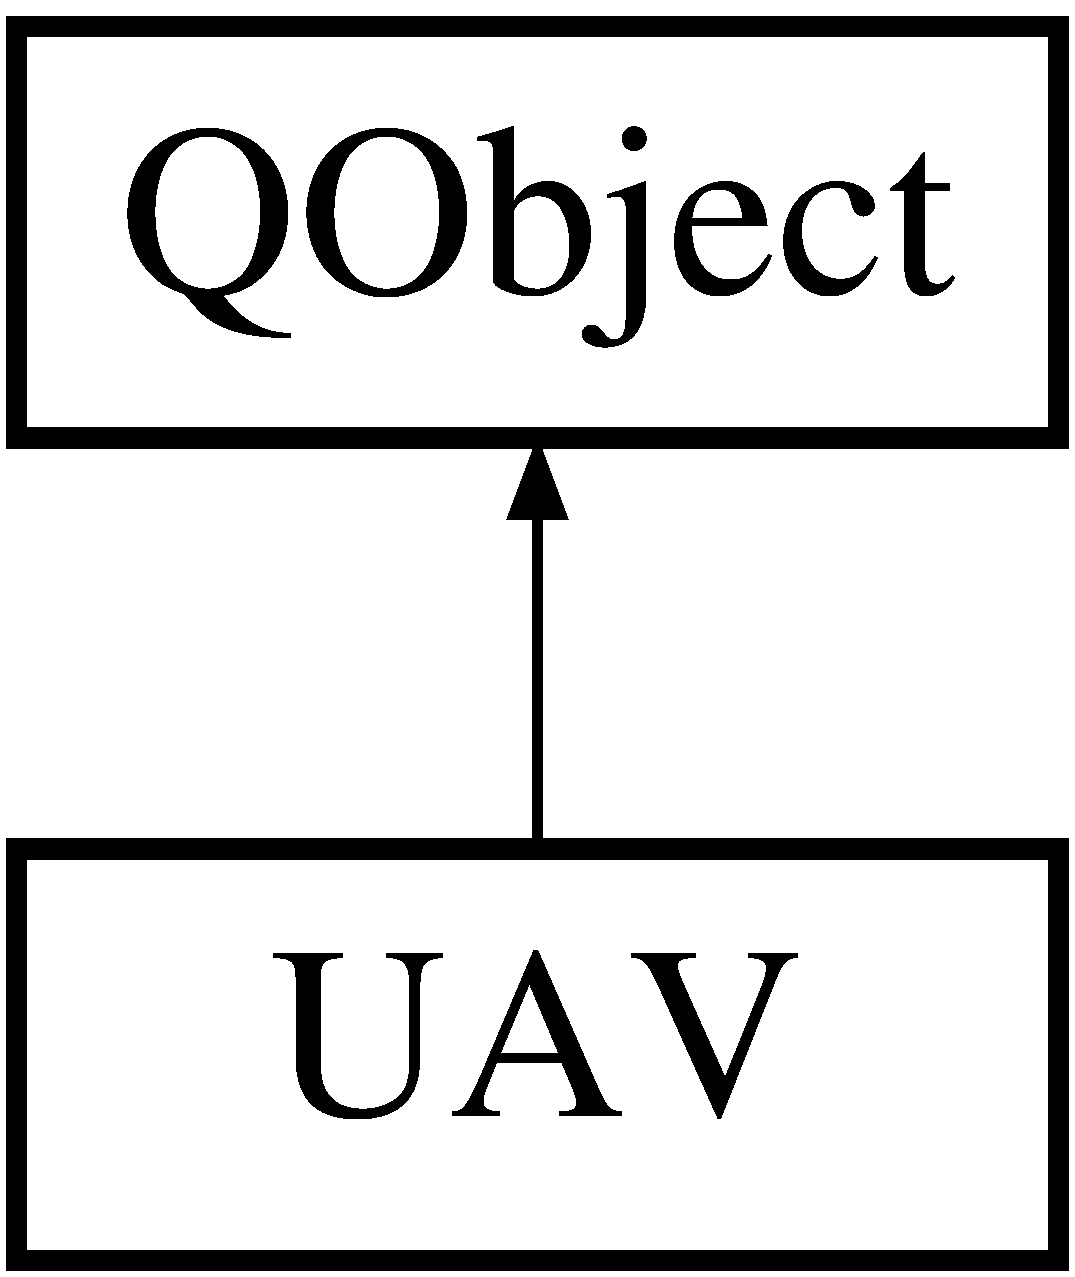
\includegraphics[height=2.000000cm]{d7/dd4/a00013}
\end{center}
\end{figure}
\subsection*{Public Slots}
\subsection*{Signals}
\subsection*{Public Member Functions}
\subsection*{Static Public Member Functions}
\subsection*{Private Member Functions}
\subsection*{Private Attributes}
\subsection*{Static Private Attributes}


\subsection{Detailed Description}


\subsection{Constructor \& Destructor Documentation}
\hypertarget{a00013_a8427a6accf01645a01805f302374356e}{\index{U\-A\-V@{U\-A\-V}!U\-A\-V@{U\-A\-V}}
\index{U\-A\-V@{U\-A\-V}!UAV@{U\-A\-V}}
\subsubsection[{U\-A\-V}]{\setlength{\rightskip}{0pt plus 5cm}{\bf U\-A\-V} (
\begin{DoxyParamCaption}
{}
\end{DoxyParamCaption}
)\hspace{0.3cm}{\ttfamily [private]}}}\label{a00013_a8427a6accf01645a01805f302374356e}


Constructor. 


\begin{DoxyParams}{Parameters}
{\em none} & \\
\hline
\end{DoxyParams}

\begin{DoxyExceptions}{Exceptions}
{\em none} & \\
\hline
\end{DoxyExceptions}
\begin{DoxyReturn}{Returns}
\hyperlink{a00013}{U\-A\-V} instance 
\end{DoxyReturn}

\begin{DoxyCode}
6 \{
7     \hyperlink{a00013_a0af541d1b4b8c59e4385c003e377b746}{m\_pPosition} = \textcolor{keyword}{new} \hyperlink{a00006}{LatLongCoord}();
8     \hyperlink{a00013_a79a2bd07a373f3b0042e6c2dc0e51fc0}{m\_dAltitude} = 0;
9     \hyperlink{a00013_a610bb35047703e6c2c0176285cd09312}{m\_dHeading} = 0;
10 
11     connect(\hyperlink{a00007_adb2b1b18fad4caaafde371f991525f38}{LogReplayControl::getInstance}(), SIGNAL(
      \hyperlink{a00013_a04e801b333f118c8877267b1797cfe24}{geolocation}(\textcolor{keywordtype}{double}, \textcolor{keywordtype}{double}, \textcolor{keywordtype}{double}, \textcolor{keywordtype}{double})), 
12         \textcolor{keyword}{this}, SLOT(\hyperlink{a00013_a04e801b333f118c8877267b1797cfe24}{geolocation}(\textcolor{keywordtype}{double}, \textcolor{keywordtype}{double}, \textcolor{keywordtype}{double}, \textcolor{keywordtype}{double})));
13     connect(\hyperlink{a00007_adb2b1b18fad4caaafde371f991525f38}{LogReplayControl::getInstance}(), SIGNAL(
      \hyperlink{a00013_aa3c54f0958638486df2b69a9b53c5d7f}{updateHeading}(\textcolor{keywordtype}{double})), \textcolor{keyword}{this}, SLOT(\hyperlink{a00013_aa3c54f0958638486df2b69a9b53c5d7f}{updateHeading}(\textcolor{keywordtype}{double})));
14 \}
\end{DoxyCode}
\hypertarget{a00013_a3e47a4e15cb6bb643cc80f6ec0880280}{\index{U\-A\-V@{U\-A\-V}!$\sim$\-U\-A\-V@{$\sim$\-U\-A\-V}}
\index{$\sim$\-U\-A\-V@{$\sim$\-U\-A\-V}!UAV@{U\-A\-V}}
\subsubsection[{$\sim$\-U\-A\-V}]{\setlength{\rightskip}{0pt plus 5cm}$\sim${\bf U\-A\-V} (
\begin{DoxyParamCaption}
{}
\end{DoxyParamCaption}
)\hspace{0.3cm}{\ttfamily [private]}}}\label{a00013_a3e47a4e15cb6bb643cc80f6ec0880280}


Destructor. 


\begin{DoxyParams}{Parameters}
{\em none} & \\
\hline
\end{DoxyParams}

\begin{DoxyExceptions}{Exceptions}
{\em none} & \\
\hline
\end{DoxyExceptions}
\begin{DoxyReturn}{Returns}
none 
\end{DoxyReturn}

\begin{DoxyCode}
26 \{
27     \textcolor{keyword}{delete} \hyperlink{a00013_a0af541d1b4b8c59e4385c003e377b746}{m\_pPosition};
28 \}
\end{DoxyCode}


\subsection{Member Function Documentation}
\hypertarget{a00013_a04e801b333f118c8877267b1797cfe24}{\index{U\-A\-V@{U\-A\-V}!geolocation@{geolocation}}
\index{geolocation@{geolocation}!UAV@{U\-A\-V}}
\subsubsection[{geolocation}]{\setlength{\rightskip}{0pt plus 5cm}void geolocation (
\begin{DoxyParamCaption}
\item[{double}]{p\-\_\-f\-Latitude, }
\item[{double}]{p\-\_\-f\-Longitude, }
\item[{double}]{p\-\_\-f\-Altitude, }
\item[{double}]{p\-\_\-f\-Heading}
\end{DoxyParamCaption}
)\hspace{0.3cm}{\ttfamily [slot]}}}\label{a00013_a04e801b333f118c8877267b1797cfe24}


geolocation update slot 


\begin{DoxyParams}{Parameters}
{\em p\-\_\-f\-Latitude} & latitude double \\
\hline
{\em p\-\_\-f\-Longitude} & longitude double \\
\hline
{\em p\-\_\-f\-Altitude} & altitude double \\
\hline
{\em p\-\_\-f\-Heading} & \char`\"{}false\char`\"{} heading double \\
\hline
\end{DoxyParams}

\begin{DoxyExceptions}{Exceptions}
{\em none} & \\
\hline
\end{DoxyExceptions}
\begin{DoxyReturn}{Returns}
none 
\end{DoxyReturn}

\begin{DoxyCode}
93 \{
94     \hyperlink{a00013_ac967c692f2002391c7210139dae74c9b}{setAltitude}(p\_fAltitude);
95     \hyperlink{a00013_ad4a7c4bae5c3e6d868a9441afbc1269a}{setCoordinates}(\textcolor{keyword}{new} \hyperlink{a00006}{LatLongCoord}(p\_fLatitude, p\_fLongitude));
96 
97     emit \hyperlink{a00013_aefff1faa5888fec11aae0f1039cf2cad}{positionChanged}();
98 \}
\end{DoxyCode}
\hypertarget{a00013_a6f20aa9c433a4f132a1720becc864a2b}{\index{U\-A\-V@{U\-A\-V}!get\-Altitude@{get\-Altitude}}
\index{get\-Altitude@{get\-Altitude}!UAV@{U\-A\-V}}
\subsubsection[{get\-Altitude}]{\setlength{\rightskip}{0pt plus 5cm}double get\-Altitude (
\begin{DoxyParamCaption}
{}
\end{DoxyParamCaption}
)}}\label{a00013_a6f20aa9c433a4f132a1720becc864a2b}


\hyperlink{a00013}{U\-A\-V} altitude getter. 


\begin{DoxyParams}{Parameters}
{\em none} & \\
\hline
\end{DoxyParams}

\begin{DoxyExceptions}{Exceptions}
{\em none} & \\
\hline
\end{DoxyExceptions}
\begin{DoxyReturn}{Returns}
altitude in meters double 
\end{DoxyReturn}

\begin{DoxyCode}
78 \{
79     \textcolor{keywordflow}{return} \hyperlink{a00013_a79a2bd07a373f3b0042e6c2dc0e51fc0}{m\_dAltitude};
80 \}
\end{DoxyCode}
\hypertarget{a00013_a8aaef3ba118d70f729ec23dee71755a7}{\index{U\-A\-V@{U\-A\-V}!get\-Coordinates@{get\-Coordinates}}
\index{get\-Coordinates@{get\-Coordinates}!UAV@{U\-A\-V}}
\subsubsection[{get\-Coordinates}]{\setlength{\rightskip}{0pt plus 5cm}{\bf Lat\-Long\-Coord} $\ast$ get\-Coordinates (
\begin{DoxyParamCaption}
{}
\end{DoxyParamCaption}
)}}\label{a00013_a8aaef3ba118d70f729ec23dee71755a7}


\hyperlink{a00013}{U\-A\-V} coordinates getter. 


\begin{DoxyParams}{Parameters}
{\em none} & \\
\hline
\end{DoxyParams}

\begin{DoxyExceptions}{Exceptions}
{\em none} & \\
\hline
\end{DoxyExceptions}
\begin{DoxyReturn}{Returns}
latitude / longitude coordinates in decimal degrees Lat\-Long\-Coord$\ast$ 
\end{DoxyReturn}

\begin{DoxyCode}
73 \{
74     \textcolor{keywordflow}{return} \hyperlink{a00013_a0af541d1b4b8c59e4385c003e377b746}{m\_pPosition};
75 \}
\end{DoxyCode}
\hypertarget{a00013_a8c56441519ab3fa6a971bc898106adc4}{\index{U\-A\-V@{U\-A\-V}!get\-Heading@{get\-Heading}}
\index{get\-Heading@{get\-Heading}!UAV@{U\-A\-V}}
\subsubsection[{get\-Heading}]{\setlength{\rightskip}{0pt plus 5cm}double get\-Heading (
\begin{DoxyParamCaption}
{}
\end{DoxyParamCaption}
)}}\label{a00013_a8c56441519ab3fa6a971bc898106adc4}


\hyperlink{a00013}{U\-A\-V} heading getter. 


\begin{DoxyParams}{Parameters}
{\em none} & \\
\hline
\end{DoxyParams}

\begin{DoxyExceptions}{Exceptions}
{\em none} & \\
\hline
\end{DoxyExceptions}
\begin{DoxyReturn}{Returns}
heading in degrees double 
\end{DoxyReturn}

\begin{DoxyCode}
83 \{
84     \textcolor{keywordflow}{return} \hyperlink{a00013_a610bb35047703e6c2c0176285cd09312}{m\_dHeading};
85 \}
\end{DoxyCode}
\hypertarget{a00013_ae1d662c26106ff9692252346d578e8fa}{\index{U\-A\-V@{U\-A\-V}!get\-Height@{get\-Height}}
\index{get\-Height@{get\-Height}!UAV@{U\-A\-V}}
\subsubsection[{get\-Height}]{\setlength{\rightskip}{0pt plus 5cm}double get\-Height (
\begin{DoxyParamCaption}
{}
\end{DoxyParamCaption}
)}}\label{a00013_ae1d662c26106ff9692252346d578e8fa}


\hyperlink{a00013}{U\-A\-V} height getter. 


\begin{DoxyParams}{Parameters}
{\em none} & \\
\hline
\end{DoxyParams}

\begin{DoxyExceptions}{Exceptions}
{\em none} & \\
\hline
\end{DoxyExceptions}
\begin{DoxyReturn}{Returns}
heading in degrees double 
\end{DoxyReturn}

\begin{DoxyCode}
88 \{
89     \textcolor{keywordflow}{return} \hyperlink{a00013_a56427301298e19fe48b131d43376abce}{m\_dHeight};
90 \}
\end{DoxyCode}
\hypertarget{a00013_a9ea1092dbfedf1611ef659a491b7bed0}{\index{U\-A\-V@{U\-A\-V}!get\-Instance@{get\-Instance}}
\index{get\-Instance@{get\-Instance}!UAV@{U\-A\-V}}
\subsubsection[{get\-Instance}]{\setlength{\rightskip}{0pt plus 5cm}{\bf U\-A\-V} $\ast$ get\-Instance (
\begin{DoxyParamCaption}
{}
\end{DoxyParamCaption}
)\hspace{0.3cm}{\ttfamily [static]}}}\label{a00013_a9ea1092dbfedf1611ef659a491b7bed0}


\hyperlink{a00013}{U\-A\-V} instance getter. 


\begin{DoxyParams}{Parameters}
{\em none} & \\
\hline
\end{DoxyParams}

\begin{DoxyExceptions}{Exceptions}
{\em none} & \\
\hline
\end{DoxyExceptions}
\begin{DoxyReturn}{Returns}
\hyperlink{a00013}{U\-A\-V} pointer U\-A\-V$\ast$ 
\end{DoxyReturn}

\begin{DoxyCode}
31 \{
32     \textcolor{keywordflow}{if} (\hyperlink{a00013_a07b6432074b71e811b0b6eb21b94e835}{singleton} == NULL)
33     \{
34         \hyperlink{a00013_a07b6432074b71e811b0b6eb21b94e835}{singleton} = \textcolor{keyword}{new} \hyperlink{a00013_a8427a6accf01645a01805f302374356e}{UAV}();
35     \}
36 
37     \textcolor{keywordflow}{return} \hyperlink{a00013_a07b6432074b71e811b0b6eb21b94e835}{singleton};
38 \}
\end{DoxyCode}
\hypertarget{a00013_aae9d52caad9fb2892deeb25596cfd2ab}{\index{U\-A\-V@{U\-A\-V}!kill@{kill}}
\index{kill@{kill}!UAV@{U\-A\-V}}
\subsubsection[{kill}]{\setlength{\rightskip}{0pt plus 5cm}void kill (
\begin{DoxyParamCaption}
{}
\end{DoxyParamCaption}
)\hspace{0.3cm}{\ttfamily [static]}}}\label{a00013_aae9d52caad9fb2892deeb25596cfd2ab}


\hyperlink{a00013}{U\-A\-V} instance killer. 


\begin{DoxyParams}{Parameters}
{\em none} & \\
\hline
\end{DoxyParams}

\begin{DoxyExceptions}{Exceptions}
{\em none} & \\
\hline
\end{DoxyExceptions}
\begin{DoxyReturn}{Returns}
none 
\end{DoxyReturn}

\begin{DoxyCode}
17 \{
18     \textcolor{keywordflow}{if} (\hyperlink{a00013_a07b6432074b71e811b0b6eb21b94e835}{singleton} != NULL)
19     \{
20         \textcolor{keyword}{delete} \hyperlink{a00013_a07b6432074b71e811b0b6eb21b94e835}{singleton};
21         \hyperlink{a00013_a07b6432074b71e811b0b6eb21b94e835}{singleton} = NULL;
22     \}
23 \}
\end{DoxyCode}
\hypertarget{a00013_aefff1faa5888fec11aae0f1039cf2cad}{\index{U\-A\-V@{U\-A\-V}!position\-Changed@{position\-Changed}}
\index{position\-Changed@{position\-Changed}!UAV@{U\-A\-V}}
\subsubsection[{position\-Changed}]{\setlength{\rightskip}{0pt plus 5cm}void position\-Changed (
\begin{DoxyParamCaption}
{}
\end{DoxyParamCaption}
)\hspace{0.3cm}{\ttfamily [signal]}}}\label{a00013_aefff1faa5888fec11aae0f1039cf2cad}


Position changed event signal. 


\begin{DoxyParams}{Parameters}
{\em none} & \\
\hline
\end{DoxyParams}

\begin{DoxyExceptions}{Exceptions}
{\em none} & \\
\hline
\end{DoxyExceptions}
\begin{DoxyReturn}{Returns}
none 
\end{DoxyReturn}
\hypertarget{a00013_ac967c692f2002391c7210139dae74c9b}{\index{U\-A\-V@{U\-A\-V}!set\-Altitude@{set\-Altitude}}
\index{set\-Altitude@{set\-Altitude}!UAV@{U\-A\-V}}
\subsubsection[{set\-Altitude}]{\setlength{\rightskip}{0pt plus 5cm}void set\-Altitude (
\begin{DoxyParamCaption}
\item[{double}]{p\-\_\-d\-Altitude}
\end{DoxyParamCaption}
)}}\label{a00013_ac967c692f2002391c7210139dae74c9b}


\hyperlink{a00013}{U\-A\-V} altitude setter. 


\begin{DoxyParams}{Parameters}
{\em p\-\_\-d\-Altitude} & new altitude double \\
\hline
\end{DoxyParams}

\begin{DoxyExceptions}{Exceptions}
{\em none} & \\
\hline
\end{DoxyExceptions}
\begin{DoxyReturn}{Returns}
none 
\end{DoxyReturn}

\begin{DoxyCode}
47 \{
48     \hyperlink{a00013_a79a2bd07a373f3b0042e6c2dc0e51fc0}{m\_dAltitude} = p\_dAltitude;
49 \}
\end{DoxyCode}
\hypertarget{a00013_ad4a7c4bae5c3e6d868a9441afbc1269a}{\index{U\-A\-V@{U\-A\-V}!set\-Coordinates@{set\-Coordinates}}
\index{set\-Coordinates@{set\-Coordinates}!UAV@{U\-A\-V}}
\subsubsection[{set\-Coordinates}]{\setlength{\rightskip}{0pt plus 5cm}void set\-Coordinates (
\begin{DoxyParamCaption}
\item[{{\bf Lat\-Long\-Coord} $\ast$}]{p\-\_\-p\-Position}
\end{DoxyParamCaption}
)}}\label{a00013_ad4a7c4bae5c3e6d868a9441afbc1269a}


\hyperlink{a00013}{U\-A\-V} coordinates setter. 


\begin{DoxyParams}{Parameters}
{\em p\-\_\-p\-Position} & new G\-P\-S coordinates Lat\-Long\-Coord$\ast$ \\
\hline
\end{DoxyParams}

\begin{DoxyExceptions}{Exceptions}
{\em none} & \\
\hline
\end{DoxyExceptions}
\begin{DoxyReturn}{Returns}
none 
\end{DoxyReturn}

\begin{DoxyCode}
41 \{
42     \hyperlink{a00013_a0af541d1b4b8c59e4385c003e377b746}{m\_pPosition}->\hyperlink{a00006_aceb619fe57529d898748a11e4fc4985d}{setCoordinates}(p\_pPosition->
      \hyperlink{a00006_a555fe9c52a678f22d66b31358566cfe9}{getLatitude}(), p\_pPosition->\hyperlink{a00006_aeca2669cb6715159606e844ab6a77bbf}{getLongitude}());
43     emit \hyperlink{a00013_aefff1faa5888fec11aae0f1039cf2cad}{positionChanged}();
44 \}
\end{DoxyCode}
\hypertarget{a00013_a7d62e844db7219c9230c5a65377ae8a4}{\index{U\-A\-V@{U\-A\-V}!set\-Heading@{set\-Heading}}
\index{set\-Heading@{set\-Heading}!UAV@{U\-A\-V}}
\subsubsection[{set\-Heading}]{\setlength{\rightskip}{0pt plus 5cm}void set\-Heading (
\begin{DoxyParamCaption}
\item[{double}]{p\-\_\-d\-Heading}
\end{DoxyParamCaption}
)}}\label{a00013_a7d62e844db7219c9230c5a65377ae8a4}


\hyperlink{a00013}{U\-A\-V} heading setter. 


\begin{DoxyParams}{Parameters}
{\em p\-\_\-d\-Heading} & new heading double \\
\hline
\end{DoxyParams}

\begin{DoxyExceptions}{Exceptions}
{\em none} & \\
\hline
\end{DoxyExceptions}
\begin{DoxyReturn}{Returns}
none 
\end{DoxyReturn}

\begin{DoxyCode}
52 \{
53     \textcolor{keywordflow}{if}(p\_dHeading > 360)
54     \{
55         \hyperlink{a00013_a610bb35047703e6c2c0176285cd09312}{m\_dHeading} = p\_dHeading - 360;
56     \}
57     \textcolor{keywordflow}{else} \textcolor{keywordflow}{if} (p\_dHeading < 0)
58     \{
59         \hyperlink{a00013_a610bb35047703e6c2c0176285cd09312}{m\_dHeading} = 360 + p\_dHeading;
60     \}
61     \textcolor{keywordflow}{else}
62     \{
63         \hyperlink{a00013_a610bb35047703e6c2c0176285cd09312}{m\_dHeading} = p\_dHeading;
64     \}
65 \}
\end{DoxyCode}
\hypertarget{a00013_af5b10f1aa2f28ed0c42d4f47efb693e9}{\index{U\-A\-V@{U\-A\-V}!set\-Height@{set\-Height}}
\index{set\-Height@{set\-Height}!UAV@{U\-A\-V}}
\subsubsection[{set\-Height}]{\setlength{\rightskip}{0pt plus 5cm}void set\-Height (
\begin{DoxyParamCaption}
\item[{double}]{p\-\_\-d\-Height}
\end{DoxyParamCaption}
)}}\label{a00013_af5b10f1aa2f28ed0c42d4f47efb693e9}


\hyperlink{a00013}{U\-A\-V} height setter. 


\begin{DoxyParams}{Parameters}
{\em p\-\_\-d\-Heading} & new heading double \\
\hline
\end{DoxyParams}

\begin{DoxyExceptions}{Exceptions}
{\em none} & \\
\hline
\end{DoxyExceptions}
\begin{DoxyReturn}{Returns}
none 
\end{DoxyReturn}

\begin{DoxyCode}
68 \{
69     \hyperlink{a00013_a56427301298e19fe48b131d43376abce}{m\_dHeight} = p\_dHeight;
70 \}
\end{DoxyCode}
\hypertarget{a00013_aa3c54f0958638486df2b69a9b53c5d7f}{\index{U\-A\-V@{U\-A\-V}!update\-Heading@{update\-Heading}}
\index{update\-Heading@{update\-Heading}!UAV@{U\-A\-V}}
\subsubsection[{update\-Heading}]{\setlength{\rightskip}{0pt plus 5cm}void update\-Heading (
\begin{DoxyParamCaption}
\item[{double}]{p\-\_\-p\-Value}
\end{DoxyParamCaption}
)\hspace{0.3cm}{\ttfamily [slot]}}}\label{a00013_aa3c54f0958638486df2b69a9b53c5d7f}


\char`\"{}real\char`\"{} heading update slot 


\begin{DoxyParams}{Parameters}
{\em p\-\_\-p\-Value} & \char`\"{}real\char`\"{} heading value double \\
\hline
\end{DoxyParams}

\begin{DoxyExceptions}{Exceptions}
{\em none} & \\
\hline
\end{DoxyExceptions}
\begin{DoxyReturn}{Returns}
none 
\end{DoxyReturn}

\begin{DoxyCode}
101 \{
102     \hyperlink{a00013_a7d62e844db7219c9230c5a65377ae8a4}{setHeading}(p\_pValue);
103 \}
\end{DoxyCode}
\hypertarget{a00013_a5114b66563f0437e0f1eac070557cb4c}{\index{U\-A\-V@{U\-A\-V}!update\-Height@{update\-Height}}
\index{update\-Height@{update\-Height}!UAV@{U\-A\-V}}
\subsubsection[{update\-Height}]{\setlength{\rightskip}{0pt plus 5cm}void update\-Height (
\begin{DoxyParamCaption}
\item[{double}]{p\-\_\-p\-Value}
\end{DoxyParamCaption}
)\hspace{0.3cm}{\ttfamily [slot]}}}\label{a00013_a5114b66563f0437e0f1eac070557cb4c}


Height (from ground) update slot. 


\begin{DoxyParams}{Parameters}
{\em p\-\_\-p\-Value} & \char`\"{}real\char`\"{} heading value double \\
\hline
\end{DoxyParams}

\begin{DoxyExceptions}{Exceptions}
{\em none} & \\
\hline
\end{DoxyExceptions}
\begin{DoxyReturn}{Returns}
none 
\end{DoxyReturn}

\begin{DoxyCode}
106 \{
107     \hyperlink{a00013_af5b10f1aa2f28ed0c42d4f47efb693e9}{setHeight}(p\_pValue);
108 \}
\end{DoxyCode}


\subsection{Field Documentation}
\hypertarget{a00013_a79a2bd07a373f3b0042e6c2dc0e51fc0}{\index{U\-A\-V@{U\-A\-V}!m\-\_\-d\-Altitude@{m\-\_\-d\-Altitude}}
\index{m\-\_\-d\-Altitude@{m\-\_\-d\-Altitude}!UAV@{U\-A\-V}}
\subsubsection[{m\-\_\-d\-Altitude}]{\setlength{\rightskip}{0pt plus 5cm}double m\-\_\-d\-Altitude\hspace{0.3cm}{\ttfamily [private]}}}\label{a00013_a79a2bd07a373f3b0042e6c2dc0e51fc0}
\hypertarget{a00013_a610bb35047703e6c2c0176285cd09312}{\index{U\-A\-V@{U\-A\-V}!m\-\_\-d\-Heading@{m\-\_\-d\-Heading}}
\index{m\-\_\-d\-Heading@{m\-\_\-d\-Heading}!UAV@{U\-A\-V}}
\subsubsection[{m\-\_\-d\-Heading}]{\setlength{\rightskip}{0pt plus 5cm}double m\-\_\-d\-Heading\hspace{0.3cm}{\ttfamily [private]}}}\label{a00013_a610bb35047703e6c2c0176285cd09312}
\hypertarget{a00013_a56427301298e19fe48b131d43376abce}{\index{U\-A\-V@{U\-A\-V}!m\-\_\-d\-Height@{m\-\_\-d\-Height}}
\index{m\-\_\-d\-Height@{m\-\_\-d\-Height}!UAV@{U\-A\-V}}
\subsubsection[{m\-\_\-d\-Height}]{\setlength{\rightskip}{0pt plus 5cm}double m\-\_\-d\-Height\hspace{0.3cm}{\ttfamily [private]}}}\label{a00013_a56427301298e19fe48b131d43376abce}
\hypertarget{a00013_a0af541d1b4b8c59e4385c003e377b746}{\index{U\-A\-V@{U\-A\-V}!m\-\_\-p\-Position@{m\-\_\-p\-Position}}
\index{m\-\_\-p\-Position@{m\-\_\-p\-Position}!UAV@{U\-A\-V}}
\subsubsection[{m\-\_\-p\-Position}]{\setlength{\rightskip}{0pt plus 5cm}{\bf Lat\-Long\-Coord}$\ast$ m\-\_\-p\-Position\hspace{0.3cm}{\ttfamily [private]}}}\label{a00013_a0af541d1b4b8c59e4385c003e377b746}
\hypertarget{a00013_a07b6432074b71e811b0b6eb21b94e835}{\index{U\-A\-V@{U\-A\-V}!singleton@{singleton}}
\index{singleton@{singleton}!UAV@{U\-A\-V}}
\subsubsection[{singleton}]{\setlength{\rightskip}{0pt plus 5cm}{\bf U\-A\-V} $\ast$ singleton = N\-U\-L\-L\hspace{0.3cm}{\ttfamily [static]}, {\ttfamily [private]}}}\label{a00013_a07b6432074b71e811b0b6eb21b94e835}


The documentation for this class was generated from the following files\-:\begin{DoxyCompactItemize}
\item 
\hyperlink{a00039}{U\-A\-V.\-h}\item 
\hyperlink{a00038}{U\-A\-V.\-cpp}\end{DoxyCompactItemize}

\hypertarget{a00014}{\section{U\-A\-V\-Logger Class Reference}
\label{a00014}\index{U\-A\-V\-Logger@{U\-A\-V\-Logger}}
}


{\ttfamily \#include \char`\"{}U\-A\-V\-Logger.\-h\char`\"{}}

Inheritance diagram for U\-A\-V\-Logger\-:\begin{figure}[H]
\begin{center}
\leavevmode
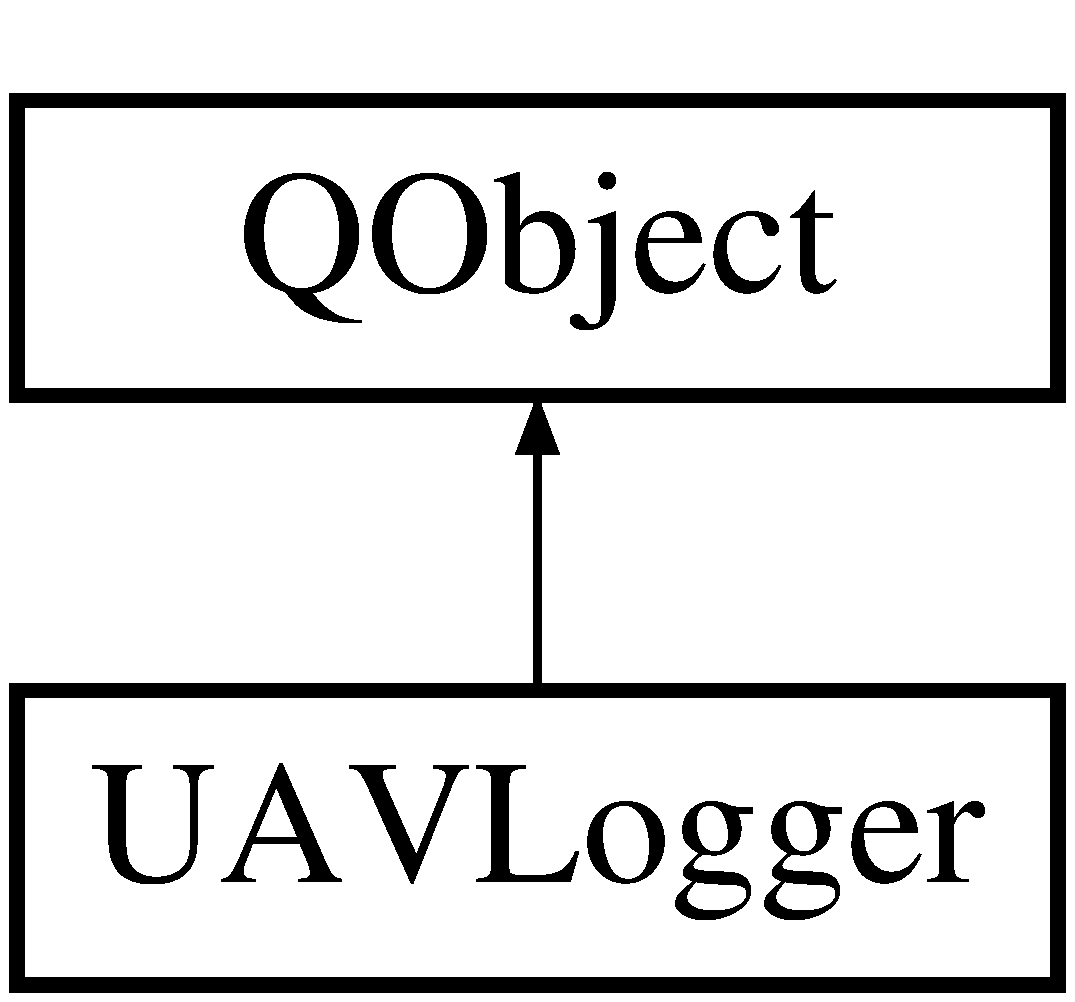
\includegraphics[height=2.000000cm]{d2/de7/a00014}
\end{center}
\end{figure}
\subsection*{Public Member Functions}
\subsection*{Private Attributes}


\subsection{Detailed Description}


\subsection{Constructor \& Destructor Documentation}
\hypertarget{a00014_a4fcbf4323f603bd19d67a2b78495d915}{\index{U\-A\-V\-Logger@{U\-A\-V\-Logger}!U\-A\-V\-Logger@{U\-A\-V\-Logger}}
\index{U\-A\-V\-Logger@{U\-A\-V\-Logger}!UAVLogger@{U\-A\-V\-Logger}}
\subsubsection[{U\-A\-V\-Logger}]{\setlength{\rightskip}{0pt plus 5cm}{\bf U\-A\-V\-Logger} (
\begin{DoxyParamCaption}
{}
\end{DoxyParamCaption}
)}}\label{a00014_a4fcbf4323f603bd19d67a2b78495d915}


Constructor. 


\begin{DoxyParams}{Parameters}
{\em none} & \\
\hline
\end{DoxyParams}

\begin{DoxyExceptions}{Exceptions}
{\em none} & \\
\hline
\end{DoxyExceptions}
\begin{DoxyReturn}{Returns}
\hyperlink{a00014}{U\-A\-V\-Logger} instance 
\end{DoxyReturn}

\begin{DoxyCode}
5 \{
6     \hyperlink{a00014_ade1d12dae61eb3386722e7ad2c79518e}{sysFile} = \textcolor{keyword}{new} QFile(QDir::currentPath()+\textcolor{stringliteral}{"/Logs/system.log"});
7     \hyperlink{a00014_a0813d5e71c0c333ade9260e2a236b7ed}{dataFile} = \textcolor{keyword}{new} QFile(QDir::currentPath()+\textcolor{stringliteral}{"/Logs/data\_RPA.csv"});
8 
9     \hyperlink{a00014_ade1d12dae61eb3386722e7ad2c79518e}{sysFile}->open(QIODevice::WriteOnly | QIODevice::Text);
10     \hyperlink{a00014_a0813d5e71c0c333ade9260e2a236b7ed}{dataFile}->open(QIODevice::WriteOnly | QIODevice::Text);
11 
12     \hyperlink{a00014_af915a8ab61a55c6cc5564aa9f79cea25}{sysLog} = \textcolor{keyword}{new} QTextStream(\hyperlink{a00014_ade1d12dae61eb3386722e7ad2c79518e}{sysFile});
13     \hyperlink{a00014_a9d49b9bb8b1be68fb2b96cb96c9a39e6}{pollLog} = \textcolor{keyword}{new} QTextStream(\hyperlink{a00014_a0813d5e71c0c333ade9260e2a236b7ed}{dataFile});
14 
15 
16 \}
\end{DoxyCode}
\hypertarget{a00014_adf64e3a6a7ca71e188fb891a4daf730a}{\index{U\-A\-V\-Logger@{U\-A\-V\-Logger}!$\sim$\-U\-A\-V\-Logger@{$\sim$\-U\-A\-V\-Logger}}
\index{$\sim$\-U\-A\-V\-Logger@{$\sim$\-U\-A\-V\-Logger}!UAVLogger@{U\-A\-V\-Logger}}
\subsubsection[{$\sim$\-U\-A\-V\-Logger}]{\setlength{\rightskip}{0pt plus 5cm}$\sim${\bf U\-A\-V\-Logger} (
\begin{DoxyParamCaption}
{}
\end{DoxyParamCaption}
)}}\label{a00014_adf64e3a6a7ca71e188fb891a4daf730a}


Destructor. 


\begin{DoxyParams}{Parameters}
{\em none} & \\
\hline
\end{DoxyParams}

\begin{DoxyExceptions}{Exceptions}
{\em none} & \\
\hline
\end{DoxyExceptions}
\begin{DoxyReturn}{Returns}
none 
\end{DoxyReturn}

\begin{DoxyCode}
19 \{
20     \hyperlink{a00014_ade1d12dae61eb3386722e7ad2c79518e}{sysFile}->close();
21     \hyperlink{a00014_a0813d5e71c0c333ade9260e2a236b7ed}{dataFile}->close();
22 
23     \textcolor{keyword}{delete} \hyperlink{a00014_af915a8ab61a55c6cc5564aa9f79cea25}{sysLog};
24     \textcolor{keyword}{delete} \hyperlink{a00014_a9d49b9bb8b1be68fb2b96cb96c9a39e6}{pollLog};
25     \textcolor{keyword}{delete} \hyperlink{a00014_a0813d5e71c0c333ade9260e2a236b7ed}{dataFile};
26     \textcolor{keyword}{delete} \hyperlink{a00014_ade1d12dae61eb3386722e7ad2c79518e}{sysFile};
27 \}
\end{DoxyCode}


\subsection{Member Function Documentation}
\hypertarget{a00014_aeabc1d456526485e8c922a94b4bfa22d}{\index{U\-A\-V\-Logger@{U\-A\-V\-Logger}!get\-Data\-Logger\-Stream@{get\-Data\-Logger\-Stream}}
\index{get\-Data\-Logger\-Stream@{get\-Data\-Logger\-Stream}!UAVLogger@{U\-A\-V\-Logger}}
\subsubsection[{get\-Data\-Logger\-Stream}]{\setlength{\rightskip}{0pt plus 5cm}Q\-Text\-Stream $\ast$ get\-Data\-Logger\-Stream (
\begin{DoxyParamCaption}
{}
\end{DoxyParamCaption}
)}}\label{a00014_aeabc1d456526485e8c922a94b4bfa22d}


Data logger getter. 


\begin{DoxyParams}{Parameters}
{\em none} & \\
\hline
\end{DoxyParams}

\begin{DoxyExceptions}{Exceptions}
{\em none} & \\
\hline
\end{DoxyExceptions}
\begin{DoxyReturn}{Returns}
C\-Card\-Detection Q\-Text\-Stream$\ast$ 
\end{DoxyReturn}

\begin{DoxyCode}
35 \{
36     \textcolor{keywordflow}{return} \hyperlink{a00014_a9d49b9bb8b1be68fb2b96cb96c9a39e6}{pollLog};
37 \}
\end{DoxyCode}
\hypertarget{a00014_abfd62a1f4f4f584858b758c0800e9b70}{\index{U\-A\-V\-Logger@{U\-A\-V\-Logger}!get\-System\-Logger\-Stream@{get\-System\-Logger\-Stream}}
\index{get\-System\-Logger\-Stream@{get\-System\-Logger\-Stream}!UAVLogger@{U\-A\-V\-Logger}}
\subsubsection[{get\-System\-Logger\-Stream}]{\setlength{\rightskip}{0pt plus 5cm}Q\-Text\-Stream $\ast$ get\-System\-Logger\-Stream (
\begin{DoxyParamCaption}
{}
\end{DoxyParamCaption}
)}}\label{a00014_abfd62a1f4f4f584858b758c0800e9b70}


System logger getter. 


\begin{DoxyParams}{Parameters}
{\em none} & \\
\hline
\end{DoxyParams}

\begin{DoxyExceptions}{Exceptions}
{\em none} & \\
\hline
\end{DoxyExceptions}
\begin{DoxyReturn}{Returns}
System logger pointer Q\-Text\-Stream$\ast$ 
\end{DoxyReturn}

\begin{DoxyCode}
30 \{
31     \textcolor{keywordflow}{return} \hyperlink{a00014_af915a8ab61a55c6cc5564aa9f79cea25}{sysLog};
32 \}
\end{DoxyCode}


\subsection{Field Documentation}
\hypertarget{a00014_a0813d5e71c0c333ade9260e2a236b7ed}{\index{U\-A\-V\-Logger@{U\-A\-V\-Logger}!data\-File@{data\-File}}
\index{data\-File@{data\-File}!UAVLogger@{U\-A\-V\-Logger}}
\subsubsection[{data\-File}]{\setlength{\rightskip}{0pt plus 5cm}Q\-File$\ast$ data\-File\hspace{0.3cm}{\ttfamily [private]}}}\label{a00014_a0813d5e71c0c333ade9260e2a236b7ed}
\hypertarget{a00014_a9d49b9bb8b1be68fb2b96cb96c9a39e6}{\index{U\-A\-V\-Logger@{U\-A\-V\-Logger}!poll\-Log@{poll\-Log}}
\index{poll\-Log@{poll\-Log}!UAVLogger@{U\-A\-V\-Logger}}
\subsubsection[{poll\-Log}]{\setlength{\rightskip}{0pt plus 5cm}Q\-Text\-Stream$\ast$ poll\-Log\hspace{0.3cm}{\ttfamily [private]}}}\label{a00014_a9d49b9bb8b1be68fb2b96cb96c9a39e6}
\hypertarget{a00014_ade1d12dae61eb3386722e7ad2c79518e}{\index{U\-A\-V\-Logger@{U\-A\-V\-Logger}!sys\-File@{sys\-File}}
\index{sys\-File@{sys\-File}!UAVLogger@{U\-A\-V\-Logger}}
\subsubsection[{sys\-File}]{\setlength{\rightskip}{0pt plus 5cm}Q\-File$\ast$ sys\-File\hspace{0.3cm}{\ttfamily [private]}}}\label{a00014_ade1d12dae61eb3386722e7ad2c79518e}
\hypertarget{a00014_af915a8ab61a55c6cc5564aa9f79cea25}{\index{U\-A\-V\-Logger@{U\-A\-V\-Logger}!sys\-Log@{sys\-Log}}
\index{sys\-Log@{sys\-Log}!UAVLogger@{U\-A\-V\-Logger}}
\subsubsection[{sys\-Log}]{\setlength{\rightskip}{0pt plus 5cm}Q\-Text\-Stream$\ast$ sys\-Log\hspace{0.3cm}{\ttfamily [private]}}}\label{a00014_af915a8ab61a55c6cc5564aa9f79cea25}


The documentation for this class was generated from the following files\-:\begin{DoxyCompactItemize}
\item 
\hyperlink{a00041}{U\-A\-V\-Logger.\-h}\item 
\hyperlink{a00040}{U\-A\-V\-Logger.\-cpp}\end{DoxyCompactItemize}

\hypertarget{a00015}{\section{video Class Reference}
\label{a00015}\index{video@{video}}
}


{\ttfamily \#include \char`\"{}video.\-h\char`\"{}}

Inheritance diagram for video\-:\begin{figure}[H]
\begin{center}
\leavevmode
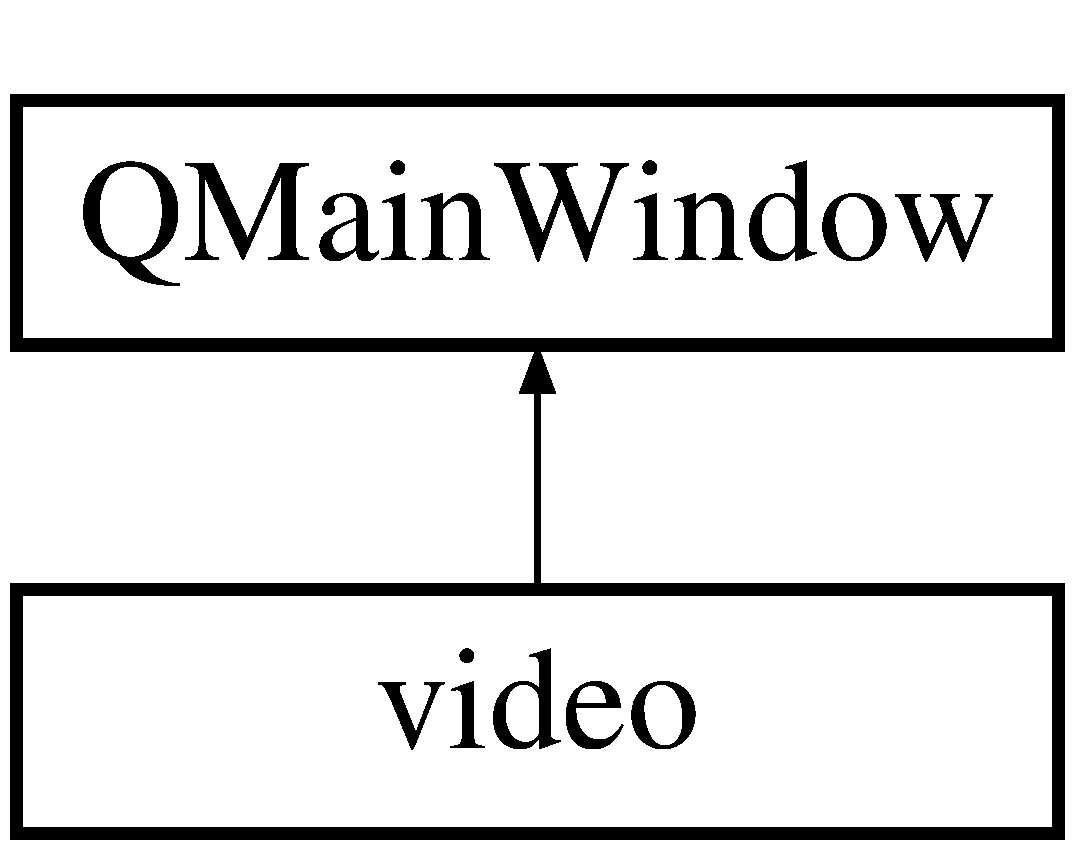
\includegraphics[height=2.000000cm]{dd/d1b/a00015}
\end{center}
\end{figure}
\subsection*{Public Slots}
\subsection*{Public Member Functions}
\subsection*{Private Attributes}


\subsection{Detailed Description}


\subsection{Constructor \& Destructor Documentation}
\hypertarget{a00015_af7ccf696656e3145c9396f15bcd91695}{\index{video@{video}!video@{video}}
\index{video@{video}!video@{video}}
\subsubsection[{video}]{\setlength{\rightskip}{0pt plus 5cm}{\bf video} (
\begin{DoxyParamCaption}
\item[{Q\-Widget $\ast$}]{parent = {\ttfamily 0}}
\end{DoxyParamCaption}
)\hspace{0.3cm}{\ttfamily [explicit]}}}\label{a00015_af7ccf696656e3145c9396f15bcd91695}

\begin{DoxyCode}
65                             :
66     QMainWindow(parent),
67     \hyperlink{a00015_a4f4e978b71511ee6fcb91ef1a4e3c17c}{ui}(\textcolor{keyword}{new} Ui::video)
68 \{
69     \hyperlink{a00042_aef1d7c2fea653fb1d729b2f40b2c2c53}{affichageList} = false ;\textcolor{comment}{//etat d'affichage de la liste du log}
70     \hyperlink{a00015_a4f4e978b71511ee6fcb91ef1a4e3c17c}{ui}->setupUi(\textcolor{keyword}{this});
71     \hyperlink{a00042_ab78e87803316b7303d0f8697c7c0f253}{place} =  \textcolor{keyword}{new} GeoDataPlacemark( \textcolor{stringliteral}{""} );
72     \hyperlink{a00042_a8b0f68f97ddd8c30ad31efa6919778ee}{document} = \textcolor{keyword}{new} GeoDataDocument();
73 
74 
75     \textcolor{comment}{//config marble}
76     \hyperlink{a00015_a4f4e978b71511ee6fcb91ef1a4e3c17c}{ui}->MarbleWidget\_smallView->setShowOverviewMap(\textcolor{keyword}{false});
77     \hyperlink{a00015_a4f4e978b71511ee6fcb91ef1a4e3c17c}{ui}->MarbleWidget\_plan->setShowOverviewMap(\textcolor{keyword}{false});
78     \hyperlink{a00015_a4f4e978b71511ee6fcb91ef1a4e3c17c}{ui}->MarbleWidget\_smallView->setShowScaleBar(\textcolor{keyword}{false});
79     \hyperlink{a00015_a4f4e978b71511ee6fcb91ef1a4e3c17c}{ui}->MarbleWidget\_smallView->setShowCompass(\textcolor{keyword}{false});
80     \hyperlink{a00015_a4f4e978b71511ee6fcb91ef1a4e3c17c}{ui}->MarbleWidget\_smallView->hide();
81 
82 
83     \textcolor{comment}{//initialisation de l'intreface}
84     \hyperlink{a00015_a4f4e978b71511ee6fcb91ef1a4e3c17c}{ui}->tableWidget->hide();
85     \hyperlink{a00015_a4f4e978b71511ee6fcb91ef1a4e3c17c}{ui}->snapShoot\_button->hide();
86     \hyperlink{a00015_a4f4e978b71511ee6fcb91ef1a4e3c17c}{ui}->actionFlight\_plan->setEnabled(\textcolor{keyword}{false});
87     \hyperlink{a00015_a4f4e978b71511ee6fcb91ef1a4e3c17c}{ui}->actionFlight\_data->setEnabled(\textcolor{keyword}{true});
88     \hyperlink{a00015_a4f4e978b71511ee6fcb91ef1a4e3c17c}{ui}->actionVideo->setEnabled(\textcolor{keyword}{true});
89     \hyperlink{a00015_a4f4e978b71511ee6fcb91ef1a4e3c17c}{ui}->listLog->hide();
90     \hyperlink{a00015_a4f4e978b71511ee6fcb91ef1a4e3c17c}{ui}->actionClear\_mission->setEnabled(\textcolor{keyword}{false});
91     \hyperlink{a00015_a4f4e978b71511ee6fcb91ef1a4e3c17c}{ui}->label\_Alt->hide();
92     \hyperlink{a00015_a4f4e978b71511ee6fcb91ef1a4e3c17c}{ui}->label\_HDG->hide();
93     \hyperlink{a00015_a4f4e978b71511ee6fcb91ef1a4e3c17c}{ui}->label\_Num\_Waypoint->hide();
94     \hyperlink{a00015_a4f4e978b71511ee6fcb91ef1a4e3c17c}{ui}->label\_Time->hide();
95     \hyperlink{a00015_a4f4e978b71511ee6fcb91ef1a4e3c17c}{ui}->lineEdit\_HDG->hide();
96     \hyperlink{a00015_a4f4e978b71511ee6fcb91ef1a4e3c17c}{ui}->lineEdit\_Alt->hide();
97     \hyperlink{a00015_a4f4e978b71511ee6fcb91ef1a4e3c17c}{ui}->timeEdit\_Mission->hide();
98     \hyperlink{a00015_a4f4e978b71511ee6fcb91ef1a4e3c17c}{ui}->line\_2->hide();
99     \hyperlink{a00015_a4f4e978b71511ee6fcb91ef1a4e3c17c}{ui}->SaveEdit\_button->hide();
100     \hyperlink{a00015_a4f4e978b71511ee6fcb91ef1a4e3c17c}{ui}->LoadData\_button->hide();
101     \hyperlink{a00015_a4f4e978b71511ee6fcb91ef1a4e3c17c}{ui}->comboBox\_ListWaypoint->hide();
102     \hyperlink{a00015_a4f4e978b71511ee6fcb91ef1a4e3c17c}{ui}->FinishEdit\_button\_2->hide();
103 
104 
105 
106     \textcolor{comment}{//signal&&slot de l'application}
107     connect(\hyperlink{a00015_a4f4e978b71511ee6fcb91ef1a4e3c17c}{ui}->actionFlight\_plan,SIGNAL(triggered()),\textcolor{keyword}{this},SLOT(
      \hyperlink{a00015_a688b7983c0da36424d5b4d10a0c007f7}{openNewWindowMain}()));
108     connect(\hyperlink{a00015_a4f4e978b71511ee6fcb91ef1a4e3c17c}{ui}->actionFlight\_data,SIGNAL(triggered()),\textcolor{keyword}{this},SLOT(
      \hyperlink{a00015_a7d0835d5762ca85bc460aeeabca018c7}{openNewWindowData}()));
109     connect(\hyperlink{a00015_a4f4e978b71511ee6fcb91ef1a4e3c17c}{ui}->actionVideo,SIGNAL(triggered()),\textcolor{keyword}{this},SLOT(\hyperlink{a00015_a03f5e63773125e14f1e32c94420ff7bf}{openNewWindowVideo}()));
110     connect(\hyperlink{a00015_a4f4e978b71511ee6fcb91ef1a4e3c17c}{ui}->actionLoad\_map,SIGNAL(triggered()),\textcolor{keyword}{this},SLOT(\hyperlink{a00015_a7225d8cbcace3eaee988a9d7724c0dbd}{openNewMap}()));
111     connect(\hyperlink{a00015_a4f4e978b71511ee6fcb91ef1a4e3c17c}{ui}->actionLoad\_mission,SIGNAL(triggered()),\textcolor{keyword}{this},SLOT(\hyperlink{a00015_a489b8f1d983d32ae8b2e5d9e29aff63a}{openMission}()));
112     connect(\hyperlink{a00015_a4f4e978b71511ee6fcb91ef1a4e3c17c}{ui}->actionClose,SIGNAL(triggered()),\textcolor{keyword}{this},SLOT(\hyperlink{a00015_a5ae591df94fc66ccb85cbb6565368bca}{close}()));
113     connect(\hyperlink{a00015_a4f4e978b71511ee6fcb91ef1a4e3c17c}{ui}->MarbleWidget\_smallView,SIGNAL(mouseClickGeoPosition(qreal,qreal,GeoDataCoordinates::Unit)
      ),\textcolor{keyword}{this},SLOT(\hyperlink{a00015_ab8446a0b12406c07562af271392ab19b}{switchToMap}()));
114     connect(\hyperlink{a00015_a4f4e978b71511ee6fcb91ef1a4e3c17c}{ui}->status\_button,SIGNAL(clicked()),\textcolor{keyword}{this},SLOT(\hyperlink{a00015_ad0f7d75c8390ef3bfcc62ad26098dacc}{afficheList}()));
115     connect(\hyperlink{a00015_a4f4e978b71511ee6fcb91ef1a4e3c17c}{ui}->led\_button,SIGNAL(clicked()),\textcolor{keyword}{this},SLOT(\hyperlink{a00015_ad0f7d75c8390ef3bfcc62ad26098dacc}{afficheList}()));
116     connect(\hyperlink{a00015_a4f4e978b71511ee6fcb91ef1a4e3c17c}{ui}->actionSave\_mission,SIGNAL(triggered()),\textcolor{keyword}{this},SLOT(\hyperlink{a00015_a816a9f0cf14cf70a29662387914071f5}{saveMission}()));
117     connect(\hyperlink{a00015_a4f4e978b71511ee6fcb91ef1a4e3c17c}{ui}->actionClear\_mission,SIGNAL(triggered()),\textcolor{keyword}{this},SLOT(\hyperlink{a00015_ac413685926a24cbbde53d1f3706a3093}{clearMission}()));
118     connect(\hyperlink{a00015_a4f4e978b71511ee6fcb91ef1a4e3c17c}{ui}->actionStart\_planning,SIGNAL(triggered()),\textcolor{keyword}{this},SLOT(
      \hyperlink{a00015_a1d75cd9cd7e205209d38efc1b47ecb13}{activateAddingPoint}()));
119     connect(\hyperlink{a00015_a4f4e978b71511ee6fcb91ef1a4e3c17c}{ui}->actionEdit\_waypoint,SIGNAL(triggered()),\textcolor{keyword}{this},SLOT(\hyperlink{a00015_a9231d60467923911b4ba0d167004588d}{editWaypoint}()));
120 
121     QPaintDevice *paintDevice = \textcolor{keyword}{this};
122    \textcolor{comment}{// QPaintEvent *evt ;}
123     QImage image;
124     \textcolor{keywordflow}{if} (!isEnabled())
125     \{
126         \textcolor{comment}{// If the globe covers fully the screen then we can use the faster}
127         \textcolor{comment}{// RGB32 as there are no translucent areas involved.}
128         QImage::Format imageFormat = ( \hyperlink{a00015_a4f4e978b71511ee6fcb91ef1a4e3c17c}{ui}->MarbleWidget\_plan->viewport()->mapCoversViewport() )
129                                      ? QImage::Format\_RGB32
130                                      : QImage::Format\_ARGB32\_Premultiplied;
131         \textcolor{comment}{// Paint to an intermediate image}
132         image = QImage( rect().size(), imageFormat );
133 
134         image.fill( Qt::transparent );
135         paintDevice = &image;
136 
137     \}
138 
139 
140 \hyperlink{a00042_a6db9a27632d51962600fe2f1debbb678}{gp} = \textcolor{keyword}{new} GeoPainter ( paintDevice, \hyperlink{a00015_a4f4e978b71511ee6fcb91ef1a4e3c17c}{ui}->MarbleWidget\_plan->viewport(), \hyperlink{a00015_a4f4e978b71511ee6fcb91ef1a4e3c17c}{ui}->MarbleWidget\_plan->
      mapQuality() );
141 \textcolor{comment}{//ui->MarbleWidget\_plan->paint( gp, evt->rect() );}
142 \hyperlink{a00015_a67857e604fad85ea53503c492a77a5a9}{drawMission}();
143 
144 \}
\end{DoxyCode}
\hypertarget{a00015_ad13b02e319297aac06bde53ec8a4b167}{\index{video@{video}!$\sim$video@{$\sim$video}}
\index{$\sim$video@{$\sim$video}!video@{video}}
\subsubsection[{$\sim$video}]{\setlength{\rightskip}{0pt plus 5cm}$\sim${\bf video} (
\begin{DoxyParamCaption}
{}
\end{DoxyParamCaption}
)}}\label{a00015_ad13b02e319297aac06bde53ec8a4b167}

\begin{DoxyCode}
147 \{
148     \textcolor{keyword}{delete} \hyperlink{a00015_a4f4e978b71511ee6fcb91ef1a4e3c17c}{ui};
149 \}
\end{DoxyCode}


\subsection{Member Function Documentation}
\hypertarget{a00015_a1d75cd9cd7e205209d38efc1b47ecb13}{\index{video@{video}!activate\-Adding\-Point@{activate\-Adding\-Point}}
\index{activate\-Adding\-Point@{activate\-Adding\-Point}!video@{video}}
\subsubsection[{activate\-Adding\-Point}]{\setlength{\rightskip}{0pt plus 5cm}void activate\-Adding\-Point (
\begin{DoxyParamCaption}
{}
\end{DoxyParamCaption}
)\hspace{0.3cm}{\ttfamily [slot]}}}\label{a00015_a1d75cd9cd7e205209d38efc1b47ecb13}

\begin{DoxyCode}
162                                \{
163     \hyperlink{a00015_a4f4e978b71511ee6fcb91ef1a4e3c17c}{ui}->actionSave\_mission->setEnabled(\textcolor{keyword}{true});
164     connect(\hyperlink{a00015_a4f4e978b71511ee6fcb91ef1a4e3c17c}{ui}->MarbleWidget\_plan,SIGNAL(mouseClickGeoPosition(qreal,qreal,GeoDataCoordinates::Unit)),\textcolor{keyword}{
      this},SLOT(\hyperlink{a00015_a070a5570eaeac36ef13715ca18be3ec9}{addPoint}(qreal,qreal,GeoDataCoordinates::Unit)));
165     \hyperlink{a00015_a4f4e978b71511ee6fcb91ef1a4e3c17c}{ui}->actionStart\_planning->setEnabled(\textcolor{keyword}{false});
166 \}
\end{DoxyCode}
\hypertarget{a00015_a070a5570eaeac36ef13715ca18be3ec9}{\index{video@{video}!add\-Point@{add\-Point}}
\index{add\-Point@{add\-Point}!video@{video}}
\subsubsection[{add\-Point}]{\setlength{\rightskip}{0pt plus 5cm}void add\-Point (
\begin{DoxyParamCaption}
\item[{qreal}]{lon, }
\item[{qreal}]{lat, }
\item[{Geo\-Data\-Coordinates\-::\-Unit}]{}
\end{DoxyParamCaption}
)\hspace{0.3cm}{\ttfamily [slot]}}}\label{a00015_a070a5570eaeac36ef13715ca18be3ec9}

\begin{DoxyCode}
268                                                                 \{
269 
270 
271   sprintf(\hyperlink{a00042_aad93f0b04d6ea6ac097124ef453bef9d}{numWpText},\textcolor{stringliteral}{"%d"},\hyperlink{a00042_ab5b110200d9f08e5d10a2549f54073c9}{num\_waypoint});
272   \hyperlink{a00042_a57c52213e1c32a667a5963a122e0a23b}{temp} = string(\hyperlink{a00042_aad93f0b04d6ea6ac097124ef453bef9d}{numWpText});
273   \hyperlink{a00042_aa6011e6576184fcd9e0841fdffbaa826}{textNumWaypoint} = \textcolor{stringliteral}{"# "} + \hyperlink{a00042_a57c52213e1c32a667a5963a122e0a23b}{temp} ;
274   \hyperlink{a00042_add3cc0473ea4a2ff453620e16ac24056}{qstr} = QString::fromStdString(\hyperlink{a00042_aa6011e6576184fcd9e0841fdffbaa826}{textNumWaypoint});
275 
276   \textcolor{comment}{// Access the shared route request (start, destination and parameters)}
277   \hyperlink{a00042_a02d3f124c170b0126dab54f6e5a18dae}{manager} = \hyperlink{a00015_a4f4e978b71511ee6fcb91ef1a4e3c17c}{ui}->MarbleWidget\_plan->model()->routingManager();
278   \hyperlink{a00042_aca10b4dc402bfe3d17f1fcba33544252}{manager\_smallMap} = \hyperlink{a00015_a4f4e978b71511ee6fcb91ef1a4e3c17c}{ui}->MarbleWidget\_smallView->model()->routingManager();
279   \hyperlink{a00042_ade0ea03ae98566eaed4f7a1f331f237a}{request} = \hyperlink{a00042_a02d3f124c170b0126dab54f6e5a18dae}{manager}->routeRequest();
280   \hyperlink{a00042_aeae2fdde26f8ed9003c0cf66a1f25662}{request\_smallMap} = \hyperlink{a00042_aca10b4dc402bfe3d17f1fcba33544252}{manager\_smallMap}->routeRequest();
281 
282   \hyperlink{a00042_a99347d1261cfb39396fdc4965d16f515}{tempo} = \textcolor{keyword}{new} GeoDataCoordinates(lon,lat,0.0,GeoDataCoordinates::Radian);
283 
284  \textcolor{comment}{// add point to map}
285  \hyperlink{a00042_ade0ea03ae98566eaed4f7a1f331f237a}{request}->append( GeoDataCoordinates( lon, lat, 0.0, GeoDataCoordinates::Radian ) );
286  \hyperlink{a00042_ade0ea03ae98566eaed4f7a1f331f237a}{request}->setName(\hyperlink{a00042_ab5b110200d9f08e5d10a2549f54073c9}{num\_waypoint},\hyperlink{a00042_add3cc0473ea4a2ff453620e16ac24056}{qstr});
287  \hyperlink{a00042_aeae2fdde26f8ed9003c0cf66a1f25662}{request\_smallMap}->append(GeoDataCoordinates( lon, lat, 0.0, GeoDataCoordinates::Radian ));
288  \hyperlink{a00042_aeae2fdde26f8ed9003c0cf66a1f25662}{request\_smallMap}->setName(\hyperlink{a00042_ab5b110200d9f08e5d10a2549f54073c9}{num\_waypoint},\hyperlink{a00042_add3cc0473ea4a2ff453620e16ac24056}{qstr});
289  \hyperlink{a00042_afe5800195fe7a91ea1bad152ba9113b5}{wpListSave}.append(\textcolor{keyword}{new} \hyperlink{a00016}{waypoint}(\hyperlink{a00042_ab5b110200d9f08e5d10a2549f54073c9}{num\_waypoint},\hyperlink{a00042_a99347d1261cfb39396fdc4965d16f515}{tempo}->longitude(
      GeoDataCoordinates::Degree),\hyperlink{a00042_a99347d1261cfb39396fdc4965d16f515}{tempo}->latitude(GeoDataCoordinates::Degree),100.0,90.0,60,1,1));
290  \hyperlink{a00042_ab5b110200d9f08e5d10a2549f54073c9}{num\_waypoint}++ ;
291 
292  \hyperlink{a00015_a4f4e978b71511ee6fcb91ef1a4e3c17c}{ui}->actionEdit\_waypoint->setEnabled(\textcolor{keyword}{true});
293  \hyperlink{a00042_a8c7e45250b1eb6821dd59fb2a9a016d7}{open} = false ;
294 \}
\end{DoxyCode}
\hypertarget{a00015_ad0f7d75c8390ef3bfcc62ad26098dacc}{\index{video@{video}!affiche\-List@{affiche\-List}}
\index{affiche\-List@{affiche\-List}!video@{video}}
\subsubsection[{affiche\-List}]{\setlength{\rightskip}{0pt plus 5cm}void affiche\-List (
\begin{DoxyParamCaption}
{}
\end{DoxyParamCaption}
)\hspace{0.3cm}{\ttfamily [slot]}}}\label{a00015_ad0f7d75c8390ef3bfcc62ad26098dacc}

\begin{DoxyCode}
170 \{
171     \textcolor{keywordflow}{if} (\hyperlink{a00042_aef1d7c2fea653fb1d729b2f40b2c2c53}{affichageList}==\textcolor{keyword}{false})\{
172         \hyperlink{a00015_a4f4e978b71511ee6fcb91ef1a4e3c17c}{ui}->listLog->show();
173         \hyperlink{a00042_aef1d7c2fea653fb1d729b2f40b2c2c53}{affichageList} = true ;
174     \}
175     \textcolor{keywordflow}{else} \{
176         \hyperlink{a00015_a4f4e978b71511ee6fcb91ef1a4e3c17c}{ui}->listLog->hide();
177         \hyperlink{a00042_aef1d7c2fea653fb1d729b2f40b2c2c53}{affichageList} = false ;
178     \}
179 
180 \}
\end{DoxyCode}
\hypertarget{a00015_ac413685926a24cbbde53d1f3706a3093}{\index{video@{video}!clear\-Mission@{clear\-Mission}}
\index{clear\-Mission@{clear\-Mission}!video@{video}}
\subsubsection[{clear\-Mission}]{\setlength{\rightskip}{0pt plus 5cm}void clear\-Mission (
\begin{DoxyParamCaption}
{}
\end{DoxyParamCaption}
)\hspace{0.3cm}{\ttfamily [slot]}}}\label{a00015_ac413685926a24cbbde53d1f3706a3093}

\begin{DoxyCode}
153                         \{
154 
155     \hyperlink{a00015_a4f4e978b71511ee6fcb91ef1a4e3c17c}{ui}->MarbleWidget\_plan->model()->removeGeoData(\hyperlink{a00042_a3de39ae285a10e6655db42a1dd146c69}{lastMission});
156     \hyperlink{a00015_a4f4e978b71511ee6fcb91ef1a4e3c17c}{ui}->actionClear\_mission->setEnabled(\textcolor{keyword}{false});
157     \hyperlink{a00015_a4f4e978b71511ee6fcb91ef1a4e3c17c}{ui}->actionSave\_mission->setEnabled(\textcolor{keyword}{false});
158 
159 \}
\end{DoxyCode}
\hypertarget{a00015_a5ae591df94fc66ccb85cbb6565368bca}{\index{video@{video}!close@{close}}
\index{close@{close}!video@{video}}
\subsubsection[{close}]{\setlength{\rightskip}{0pt plus 5cm}void close (
\begin{DoxyParamCaption}
{}
\end{DoxyParamCaption}
)\hspace{0.3cm}{\ttfamily [slot]}}}\label{a00015_a5ae591df94fc66ccb85cbb6565368bca}

\begin{DoxyCode}
340 \{
341     exit(0);
342 \}
\end{DoxyCode}
\hypertarget{a00015_a67857e604fad85ea53503c492a77a5a9}{\index{video@{video}!draw\-Mission@{draw\-Mission}}
\index{draw\-Mission@{draw\-Mission}!video@{video}}
\subsubsection[{draw\-Mission}]{\setlength{\rightskip}{0pt plus 5cm}void draw\-Mission (
\begin{DoxyParamCaption}
{}
\end{DoxyParamCaption}
)\hspace{0.3cm}{\ttfamily [slot]}}}\label{a00015_a67857e604fad85ea53503c492a77a5a9}

\begin{DoxyCode}
372                        \{
373 
374     GeoDataCoordinates France( 2.2, 48.52, 0.0, GeoDataCoordinates::Degree );
375     \hyperlink{a00042_a6db9a27632d51962600fe2f1debbb678}{gp}->setPen( QColor( 0, 0, 0 ) );
376     \hyperlink{a00042_a6db9a27632d51962600fe2f1debbb678}{gp}->drawText( France, \textcolor{stringliteral}{"France"} );
377 
378     GeoDataCoordinates Canada( -77.02, 48.52, 0.0, GeoDataCoordinates::Degree );
379     \hyperlink{a00042_a6db9a27632d51962600fe2f1debbb678}{gp}->setPen( QColor( 0, 0, 0 ) );
380     \hyperlink{a00042_a6db9a27632d51962600fe2f1debbb678}{gp}->drawText( Canada, \textcolor{stringliteral}{"Canada"} );
381 
382     \textcolor{comment}{//A line from France to Canada without tessellation}
383 
384     GeoDataLineString shapeNoTessellation( NoTessellation );
385     shapeNoTessellation << France << Canada;
386 
387     \hyperlink{a00042_a6db9a27632d51962600fe2f1debbb678}{gp}->setPen( oxygenSkyBlue4 );
388     \hyperlink{a00042_a6db9a27632d51962600fe2f1debbb678}{gp}->drawPolyline( shapeNoTessellation );
389 
390     \textcolor{comment}{//The same line, but with tessellation}
391 
392     GeoDataLineString shapeTessellate( Tessellate );
393     shapeTessellate << France << Canada;
394 
395     \hyperlink{a00042_a6db9a27632d51962600fe2f1debbb678}{gp}->setPen( oxygenBrickRed4 );
396     \hyperlink{a00042_a6db9a27632d51962600fe2f1debbb678}{gp}->drawPolyline( shapeTessellate );
397 
398     \textcolor{comment}{//Now following the latitude circles}
399 
400     GeoDataLineString shapeLatitudeCircle( RespectLatitudeCircle | Tessellate );
401     shapeLatitudeCircle << France << Canada;
402 
403     \hyperlink{a00042_a6db9a27632d51962600fe2f1debbb678}{gp}->setPen( oxygenForestGreen4 );
404     \hyperlink{a00042_a6db9a27632d51962600fe2f1debbb678}{gp}->drawPolyline( shapeLatitudeCircle );
405 \}
\end{DoxyCode}
\hypertarget{a00015_a9231d60467923911b4ba0d167004588d}{\index{video@{video}!edit\-Waypoint@{edit\-Waypoint}}
\index{edit\-Waypoint@{edit\-Waypoint}!video@{video}}
\subsubsection[{edit\-Waypoint}]{\setlength{\rightskip}{0pt plus 5cm}void edit\-Waypoint (
\begin{DoxyParamCaption}
{}
\end{DoxyParamCaption}
)\hspace{0.3cm}{\ttfamily [slot]}}}\label{a00015_a9231d60467923911b4ba0d167004588d}

\begin{DoxyCode}
407                         \{
408     \hyperlink{a00015_a4f4e978b71511ee6fcb91ef1a4e3c17c}{ui}->comboBox\_ListWaypoint->show();
409     \hyperlink{a00015_a4f4e978b71511ee6fcb91ef1a4e3c17c}{ui}->LoadData\_button->show();
410     \hyperlink{a00015_a4f4e978b71511ee6fcb91ef1a4e3c17c}{ui}->label\_Num\_Waypoint->show();
411 
412     \hyperlink{a00015_a4f4e978b71511ee6fcb91ef1a4e3c17c}{ui}->actionEdit\_waypoint->setEnabled(\textcolor{keyword}{false});
413     \hyperlink{a00015_a4f4e978b71511ee6fcb91ef1a4e3c17c}{ui}->comboBox\_ListWaypoint->clear();
414 
415     \textcolor{keywordflow}{if} ( \hyperlink{a00042_a8c7e45250b1eb6821dd59fb2a9a016d7}{open} == \textcolor{keyword}{false})\{
416 
417         \textcolor{keywordflow}{for} ( \textcolor{keywordtype}{int} i = 0 ; i < \hyperlink{a00042_afe5800195fe7a91ea1bad152ba9113b5}{wpListSave}.size(); i++)\{
418             \hyperlink{a00015_a4f4e978b71511ee6fcb91ef1a4e3c17c}{ui}->comboBox\_ListWaypoint->addItem(QString::number(i+1));
419         \}
420     \}
421     \textcolor{keywordflow}{else} \{
422         \textcolor{keywordflow}{for} ( \textcolor{keywordtype}{int} i = 0 ; i < \hyperlink{a00042_a5d3a9439b166172c9c871c9a723eac19}{wpListOpen}.size(); i++)\{
423             \hyperlink{a00015_a4f4e978b71511ee6fcb91ef1a4e3c17c}{ui}->comboBox\_ListWaypoint->addItem(QString::number(i+1));
424         \}
425 
426     \}
427 
428     connect(\hyperlink{a00015_a4f4e978b71511ee6fcb91ef1a4e3c17c}{ui}->LoadData\_button,SIGNAL(clicked()),\textcolor{keyword}{this},SLOT(\hyperlink{a00015_a3ba779451a386238417fbab60f0d4db0}{loadData}()));
429 
430 
431 \}
\end{DoxyCode}
\hypertarget{a00015_a7e07a9d88a66fadd639dec3139cf9f4c}{\index{video@{video}!finish\-Edit\-Data@{finish\-Edit\-Data}}
\index{finish\-Edit\-Data@{finish\-Edit\-Data}!video@{video}}
\subsubsection[{finish\-Edit\-Data}]{\setlength{\rightskip}{0pt plus 5cm}void finish\-Edit\-Data (
\begin{DoxyParamCaption}
{}
\end{DoxyParamCaption}
)\hspace{0.3cm}{\ttfamily [slot]}}}\label{a00015_a7e07a9d88a66fadd639dec3139cf9f4c}

\begin{DoxyCode}
504                           \{
505 
506 
507     \hyperlink{a00015_a4f4e978b71511ee6fcb91ef1a4e3c17c}{ui}->label\_Alt->hide();
508     \hyperlink{a00015_a4f4e978b71511ee6fcb91ef1a4e3c17c}{ui}->label\_HDG->hide();
509     \hyperlink{a00015_a4f4e978b71511ee6fcb91ef1a4e3c17c}{ui}->label\_Num\_Waypoint->hide();
510     \hyperlink{a00015_a4f4e978b71511ee6fcb91ef1a4e3c17c}{ui}->label\_Time->hide();
511     \hyperlink{a00015_a4f4e978b71511ee6fcb91ef1a4e3c17c}{ui}->lineEdit\_HDG->hide();
512     \hyperlink{a00015_a4f4e978b71511ee6fcb91ef1a4e3c17c}{ui}->lineEdit\_Alt->hide();
513     \hyperlink{a00015_a4f4e978b71511ee6fcb91ef1a4e3c17c}{ui}->timeEdit\_Mission->hide();
514     \hyperlink{a00015_a4f4e978b71511ee6fcb91ef1a4e3c17c}{ui}->line\_2->hide();
515     \hyperlink{a00015_a4f4e978b71511ee6fcb91ef1a4e3c17c}{ui}->SaveEdit\_button->hide();
516     \hyperlink{a00015_a4f4e978b71511ee6fcb91ef1a4e3c17c}{ui}->LoadData\_button->hide();
517     \hyperlink{a00015_a4f4e978b71511ee6fcb91ef1a4e3c17c}{ui}->comboBox\_ListWaypoint->hide();
518     \hyperlink{a00015_a4f4e978b71511ee6fcb91ef1a4e3c17c}{ui}->FinishEdit\_button\_2->hide();
519     \hyperlink{a00015_a4f4e978b71511ee6fcb91ef1a4e3c17c}{ui}->actionEdit\_waypoint->setEnabled(\textcolor{keyword}{true});
520 
521 
522 \}
\end{DoxyCode}
\hypertarget{a00015_a3ba779451a386238417fbab60f0d4db0}{\index{video@{video}!load\-Data@{load\-Data}}
\index{load\-Data@{load\-Data}!video@{video}}
\subsubsection[{load\-Data}]{\setlength{\rightskip}{0pt plus 5cm}void load\-Data (
\begin{DoxyParamCaption}
{}
\end{DoxyParamCaption}
)\hspace{0.3cm}{\ttfamily [slot]}}}\label{a00015_a3ba779451a386238417fbab60f0d4db0}

\begin{DoxyCode}
433                     \{
434     \textcolor{keywordtype}{int} h ;
435     \textcolor{keywordtype}{int} m ;
436     \textcolor{keywordtype}{int} s ;
437 
438     \hyperlink{a00015_a4f4e978b71511ee6fcb91ef1a4e3c17c}{ui}->label\_Alt->show();
439     \hyperlink{a00015_a4f4e978b71511ee6fcb91ef1a4e3c17c}{ui}->label\_HDG->show();
440     \hyperlink{a00015_a4f4e978b71511ee6fcb91ef1a4e3c17c}{ui}->label\_Time->show();
441     \hyperlink{a00015_a4f4e978b71511ee6fcb91ef1a4e3c17c}{ui}->lineEdit\_Alt->show();
442     \hyperlink{a00015_a4f4e978b71511ee6fcb91ef1a4e3c17c}{ui}->lineEdit\_HDG->show();
443     \hyperlink{a00015_a4f4e978b71511ee6fcb91ef1a4e3c17c}{ui}->timeEdit\_Mission->show();
444     \hyperlink{a00015_a4f4e978b71511ee6fcb91ef1a4e3c17c}{ui}->line\_2->show();
445     \hyperlink{a00015_a4f4e978b71511ee6fcb91ef1a4e3c17c}{ui}->SaveEdit\_button->show();
446     \hyperlink{a00015_a4f4e978b71511ee6fcb91ef1a4e3c17c}{ui}->FinishEdit\_button\_2->show();
447     \hyperlink{a00015_a4f4e978b71511ee6fcb91ef1a4e3c17c}{ui}->SaveEdit\_button->setEnabled(\textcolor{keyword}{true});
448 
449     \textcolor{keywordflow}{if} ( \hyperlink{a00042_a8c7e45250b1eb6821dd59fb2a9a016d7}{open} == \textcolor{keyword}{false})\{
450         h = \hyperlink{a00042_afe5800195fe7a91ea1bad152ba9113b5}{wpListSave}[\hyperlink{a00015_a4f4e978b71511ee6fcb91ef1a4e3c17c}{ui}->comboBox\_ListWaypoint->currentIndex()]->getTime() / 3600 ;
451         m = (\hyperlink{a00042_afe5800195fe7a91ea1bad152ba9113b5}{wpListSave}[\hyperlink{a00015_a4f4e978b71511ee6fcb91ef1a4e3c17c}{ui}->comboBox\_ListWaypoint->currentIndex()]->getTime() % 3600)/60 ;
452         s = (\hyperlink{a00042_afe5800195fe7a91ea1bad152ba9113b5}{wpListSave}[\hyperlink{a00015_a4f4e978b71511ee6fcb91ef1a4e3c17c}{ui}->comboBox\_ListWaypoint->currentIndex()]->getTime() % 3600)%60  ;
453 
454        \hyperlink{a00015_a4f4e978b71511ee6fcb91ef1a4e3c17c}{ui}->lineEdit\_Alt->setText(QString::number(\hyperlink{a00042_afe5800195fe7a91ea1bad152ba9113b5}{wpListSave}[\hyperlink{a00015_a4f4e978b71511ee6fcb91ef1a4e3c17c}{ui}->comboBox\_ListWaypoint->
      currentIndex()]->getAlt()));
455        \hyperlink{a00015_a4f4e978b71511ee6fcb91ef1a4e3c17c}{ui}->lineEdit\_HDG->setText(QString::number(\hyperlink{a00042_afe5800195fe7a91ea1bad152ba9113b5}{wpListSave}[\hyperlink{a00015_a4f4e978b71511ee6fcb91ef1a4e3c17c}{ui}->comboBox\_ListWaypoint->
      currentIndex()]->getHdg()));
456        \hyperlink{a00015_a4f4e978b71511ee6fcb91ef1a4e3c17c}{ui}->timeEdit\_Mission->setTime(QTime(h,m,s,00));
457 
458     \}
459 
460     \textcolor{keywordflow}{else} \{
461         h = \hyperlink{a00042_a5d3a9439b166172c9c871c9a723eac19}{wpListOpen}[\hyperlink{a00015_a4f4e978b71511ee6fcb91ef1a4e3c17c}{ui}->comboBox\_ListWaypoint->currentIndex()]->getTime() / 3600 ;
462         m = (\hyperlink{a00042_a5d3a9439b166172c9c871c9a723eac19}{wpListOpen}[\hyperlink{a00015_a4f4e978b71511ee6fcb91ef1a4e3c17c}{ui}->comboBox\_ListWaypoint->currentIndex()]->getTime() % 3600)/60 ;
463         s = (\hyperlink{a00042_a5d3a9439b166172c9c871c9a723eac19}{wpListOpen}[\hyperlink{a00015_a4f4e978b71511ee6fcb91ef1a4e3c17c}{ui}->comboBox\_ListWaypoint->currentIndex()]->getTime() % 3600)%60  ;
464 
465        \hyperlink{a00015_a4f4e978b71511ee6fcb91ef1a4e3c17c}{ui}->lineEdit\_Alt->setText(QString::number(\hyperlink{a00042_a5d3a9439b166172c9c871c9a723eac19}{wpListOpen}[\hyperlink{a00015_a4f4e978b71511ee6fcb91ef1a4e3c17c}{ui}->comboBox\_ListWaypoint->
      currentIndex()]->getAlt()));
466        \hyperlink{a00015_a4f4e978b71511ee6fcb91ef1a4e3c17c}{ui}->lineEdit\_HDG->setText(QString::number(\hyperlink{a00042_a5d3a9439b166172c9c871c9a723eac19}{wpListOpen}[\hyperlink{a00015_a4f4e978b71511ee6fcb91ef1a4e3c17c}{ui}->comboBox\_ListWaypoint->
      currentIndex()]->getHdg()));
467        \hyperlink{a00015_a4f4e978b71511ee6fcb91ef1a4e3c17c}{ui}->timeEdit\_Mission->setTime(QTime(h,m,s,00));
468 
469     \}
470 
471     connect(\hyperlink{a00015_a4f4e978b71511ee6fcb91ef1a4e3c17c}{ui}->SaveEdit\_button,SIGNAL(clicked()),\textcolor{keyword}{this},SLOT(\hyperlink{a00015_a14a8662407eb95fe2c478c0cee351de5}{saveEditData}()));
472     connect(\hyperlink{a00015_a4f4e978b71511ee6fcb91ef1a4e3c17c}{ui}->FinishEdit\_button\_2,SIGNAL(clicked()),\textcolor{keyword}{this},SLOT(\hyperlink{a00015_a7e07a9d88a66fadd639dec3139cf9f4c}{finishEditData}()));
473 
474    \}
\end{DoxyCode}
\hypertarget{a00015_a489b8f1d983d32ae8b2e5d9e29aff63a}{\index{video@{video}!open\-Mission@{open\-Mission}}
\index{open\-Mission@{open\-Mission}!video@{video}}
\subsubsection[{open\-Mission}]{\setlength{\rightskip}{0pt plus 5cm}void open\-Mission (
\begin{DoxyParamCaption}
{}
\end{DoxyParamCaption}
)\hspace{0.3cm}{\ttfamily [slot]}}}\label{a00015_a489b8f1d983d32ae8b2e5d9e29aff63a}

\begin{DoxyCode}
183                        \{
184 
185    disconnect(\hyperlink{a00015_a4f4e978b71511ee6fcb91ef1a4e3c17c}{ui}->MarbleWidget\_plan,SIGNAL(mouseClickGeoPosition(qreal,qreal,GeoDataCoordinates::Unit)),\textcolor{keyword}{
      this},SLOT(\hyperlink{a00015_a070a5570eaeac36ef13715ca18be3ec9}{addPoint}(qreal,qreal,GeoDataCoordinates::Unit)));
186 
187     \hyperlink{a00015_a34b772573db9a14b1acb61b24709ae73}{path} = QFileDialog::getOpenFileName(\textcolor{keyword}{this}, \textcolor{stringliteral}{"Load a mission"}, \textcolor{stringliteral}{"C:/Users/mboussai/Desktop/Mohamed/Qt
       Projects/FILES/mission"}, \textcolor{stringliteral}{"KML (*.kml)"});
188     QFileInfo inputFile(\hyperlink{a00015_a34b772573db9a14b1acb61b24709ae73}{path});
189     QString file ;
190     file = \textcolor{stringliteral}{"C:/Users/mboussai/Desktop/Mohamed/Qt Projects/MARCS/MissionXML/testParse.xml"};
191 
192     \textcolor{keywordtype}{string} m ;
193     \textcolor{keywordtype}{string} nameFileOpen;
194 
195 
196     m = \hyperlink{a00015_a34b772573db9a14b1acb61b24709ae73}{path}.toUtf8().constData();
197     \textcolor{keywordtype}{size\_t} pos = m.find\_last\_of(\textcolor{stringliteral}{"/"});
198     \textcolor{keywordflow}{if}(pos != std::string::npos)\{
199 
200         nameFileOpen.assign(m.begin() + pos + 1, m.end()-4);
201     \}
202       \textcolor{keywordflow}{else}
203     \{
204       nameFileOpen = m;
205   \}
206     \textcolor{keywordtype}{string} fileNameTempOpen = \textcolor{stringliteral}{"C:/Users/mboussai/Desktop/Mohamed/Qt Projects/MARCS/MissionXML/"} + 
      nameFileOpen +\textcolor{stringliteral}{".xml"} ;
207     \hyperlink{a00042_ae55f476d1700ade204b3038b8c37f8ba}{fileOpened} =  QString::fromStdString(fileNameTempOpen);
208 
209     \textcolor{comment}{// Access the shared route request (start, destination and parameters)}
210     \hyperlink{a00042_a02d3f124c170b0126dab54f6e5a18dae}{manager} = \hyperlink{a00015_a4f4e978b71511ee6fcb91ef1a4e3c17c}{ui}->MarbleWidget\_plan->model()->routingManager();
211     \hyperlink{a00042_aca10b4dc402bfe3d17f1fcba33544252}{manager\_smallMap} = \hyperlink{a00015_a4f4e978b71511ee6fcb91ef1a4e3c17c}{ui}->MarbleWidget\_smallView->model()->routingManager();
212     \hyperlink{a00042_ade0ea03ae98566eaed4f7a1f331f237a}{request} = \hyperlink{a00042_a02d3f124c170b0126dab54f6e5a18dae}{manager}->routeRequest();
213     \hyperlink{a00042_aeae2fdde26f8ed9003c0cf66a1f25662}{request\_smallMap} = \hyperlink{a00042_aca10b4dc402bfe3d17f1fcba33544252}{manager\_smallMap}->routeRequest();
214     \hyperlink{a00042_ade0ea03ae98566eaed4f7a1f331f237a}{request}->append( GeoDataCoordinates( 0.0, 1.0, 0.0, GeoDataCoordinates::Radian ) );
215     \hyperlink{a00042_aeae2fdde26f8ed9003c0cf66a1f25662}{request\_smallMap}->append(GeoDataCoordinates( 0.0, 4.0, 0.0, GeoDataCoordinates::Radian 
      ));
216 
217     \hyperlink{a00042_ade0ea03ae98566eaed4f7a1f331f237a}{request}->clear();
218     \hyperlink{a00042_aeae2fdde26f8ed9003c0cf66a1f25662}{request\_smallMap}->clear();
219     \hyperlink{a00015_a4f4e978b71511ee6fcb91ef1a4e3c17c}{ui}->MarbleWidget\_plan->model()->addGeoDataFile( inputFile.absoluteFilePath() );
220     \hyperlink{a00015_a4f4e978b71511ee6fcb91ef1a4e3c17c}{ui}->MarbleWidget\_plan->repaint();
221     \hyperlink{a00015_a4f4e978b71511ee6fcb91ef1a4e3c17c}{ui}->MarbleWidget\_smallView->model()->addGeoDataFile( inputFile.absoluteFilePath() );
222     \hyperlink{a00042_a3de39ae285a10e6655db42a1dd146c69}{lastMission} = inputFile.absoluteFilePath();
223     \hyperlink{a00015_a4f4e978b71511ee6fcb91ef1a4e3c17c}{ui}->actionClear\_mission->setEnabled(\textcolor{keyword}{true});
224     \hyperlink{a00042_a3de39ae285a10e6655db42a1dd146c69}{lastMission} = inputFile.absoluteFilePath();
225     \hyperlink{a00015_a4f4e978b71511ee6fcb91ef1a4e3c17c}{ui}->actionStart\_planning->setEnabled(\textcolor{keyword}{true});
226 
227      \hyperlink{a00042_a5d3a9439b166172c9c871c9a723eac19}{wpListOpen} = \hyperlink{a00015_a8bd377d858dd541faf8108389a13e5ed}{myMission}.\hyperlink{a00009_af307fc09e3c8e4303ff16324d681213a}{loadMission}(\hyperlink{a00042_a5d3a9439b166172c9c871c9a723eac19}{wpListOpen},
      \hyperlink{a00042_ae55f476d1700ade204b3038b8c37f8ba}{fileOpened});
228     \hyperlink{a00015_a4f4e978b71511ee6fcb91ef1a4e3c17c}{ui}->actionEdit\_waypoint->setEnabled(\textcolor{keyword}{true});
229     \hyperlink{a00042_a8c7e45250b1eb6821dd59fb2a9a016d7}{open} = true ;
230 
231 
232 \}
\end{DoxyCode}
\hypertarget{a00015_a7225d8cbcace3eaee988a9d7724c0dbd}{\index{video@{video}!open\-New\-Map@{open\-New\-Map}}
\index{open\-New\-Map@{open\-New\-Map}!video@{video}}
\subsubsection[{open\-New\-Map}]{\setlength{\rightskip}{0pt plus 5cm}void open\-New\-Map (
\begin{DoxyParamCaption}
{}
\end{DoxyParamCaption}
)\hspace{0.3cm}{\ttfamily [slot]}}}\label{a00015_a7225d8cbcace3eaee988a9d7724c0dbd}

\begin{DoxyCode}
347 \{
348     \hyperlink{a00015_a34b772573db9a14b1acb61b24709ae73}{path} = QFileDialog::getOpenFileName(\textcolor{keyword}{this}, \textcolor{stringliteral}{"Load a map"},\textcolor{stringliteral}{"C:/Users/mboussai/Desktop/Mohamed/Qt
       Projects/FILES/map"}, \textcolor{stringliteral}{"OSM (*.osm)"});
349     QFileInfo inputFile(\hyperlink{a00015_a34b772573db9a14b1acb61b24709ae73}{path});
350 
351         \hyperlink{a00015_a4f4e978b71511ee6fcb91ef1a4e3c17c}{ui}->MarbleWidget\_plan->model()->removeGeoData(\hyperlink{a00042_ade9b9dbbdedb4e80abbaa2201ba82d05}{lastMap});
352         \hyperlink{a00015_a4f4e978b71511ee6fcb91ef1a4e3c17c}{ui}->MarbleWidget\_plan->model()->addGeoDataFile( inputFile.absoluteFilePath() );
353         \hyperlink{a00015_a4f4e978b71511ee6fcb91ef1a4e3c17c}{ui}->MarbleWidget\_smallView->model()->addGeoDataFile( inputFile.absoluteFilePath() );
354         \hyperlink{a00042_ade9b9dbbdedb4e80abbaa2201ba82d05}{lastMap} = inputFile.absoluteFilePath();
355 
356 \}
\end{DoxyCode}
\hypertarget{a00015_a7d0835d5762ca85bc460aeeabca018c7}{\index{video@{video}!open\-New\-Window\-Data@{open\-New\-Window\-Data}}
\index{open\-New\-Window\-Data@{open\-New\-Window\-Data}!video@{video}}
\subsubsection[{open\-New\-Window\-Data}]{\setlength{\rightskip}{0pt plus 5cm}void open\-New\-Window\-Data (
\begin{DoxyParamCaption}
{}
\end{DoxyParamCaption}
)\hspace{0.3cm}{\ttfamily [slot]}}}\label{a00015_a7d0835d5762ca85bc460aeeabca018c7}

\begin{DoxyCode}
312 \{
313     \hyperlink{a00015_a4f4e978b71511ee6fcb91ef1a4e3c17c}{ui}->MarbleWidget\_plan->hide();
314     \hyperlink{a00015_a4f4e978b71511ee6fcb91ef1a4e3c17c}{ui}->MarbleWidget\_smallView->hide();
315     \hyperlink{a00015_a4f4e978b71511ee6fcb91ef1a4e3c17c}{ui}->tableWidget->show();
316     \hyperlink{a00015_a4f4e978b71511ee6fcb91ef1a4e3c17c}{ui}->snapShoot\_button->hide();
317     \hyperlink{a00015_a4f4e978b71511ee6fcb91ef1a4e3c17c}{ui}->addMark\_button->hide();
318     \hyperlink{a00015_a4f4e978b71511ee6fcb91ef1a4e3c17c}{ui}->actionFlight\_plan->setEnabled(\textcolor{keyword}{true});
319     \hyperlink{a00015_a4f4e978b71511ee6fcb91ef1a4e3c17c}{ui}->actionFlight\_data->setEnabled(\textcolor{keyword}{false});
320     \hyperlink{a00015_a4f4e978b71511ee6fcb91ef1a4e3c17c}{ui}->actionVideo->setEnabled(\textcolor{keyword}{true});
321 
322 \}
\end{DoxyCode}
\hypertarget{a00015_a688b7983c0da36424d5b4d10a0c007f7}{\index{video@{video}!open\-New\-Window\-Main@{open\-New\-Window\-Main}}
\index{open\-New\-Window\-Main@{open\-New\-Window\-Main}!video@{video}}
\subsubsection[{open\-New\-Window\-Main}]{\setlength{\rightskip}{0pt plus 5cm}void open\-New\-Window\-Main (
\begin{DoxyParamCaption}
{}
\end{DoxyParamCaption}
)\hspace{0.3cm}{\ttfamily [slot]}}}\label{a00015_a688b7983c0da36424d5b4d10a0c007f7}

\begin{DoxyCode}
298 \{
299     \hyperlink{a00015_a4f4e978b71511ee6fcb91ef1a4e3c17c}{ui}->MarbleWidget\_plan->show();
300     \hyperlink{a00015_a4f4e978b71511ee6fcb91ef1a4e3c17c}{ui}->MarbleWidget\_smallView->hide();
301     \hyperlink{a00015_a4f4e978b71511ee6fcb91ef1a4e3c17c}{ui}->tableWidget->hide();
302     \hyperlink{a00015_a4f4e978b71511ee6fcb91ef1a4e3c17c}{ui}->snapShoot\_button->hide();
303     \hyperlink{a00015_a4f4e978b71511ee6fcb91ef1a4e3c17c}{ui}->addMark\_button->show();
304     \hyperlink{a00015_a4f4e978b71511ee6fcb91ef1a4e3c17c}{ui}->actionFlight\_plan->setEnabled(\textcolor{keyword}{false});
305     \hyperlink{a00015_a4f4e978b71511ee6fcb91ef1a4e3c17c}{ui}->actionFlight\_data->setEnabled(\textcolor{keyword}{true});
306     \hyperlink{a00015_a4f4e978b71511ee6fcb91ef1a4e3c17c}{ui}->actionVideo->setEnabled(\textcolor{keyword}{true});
307 
308 \}
\end{DoxyCode}
\hypertarget{a00015_a03f5e63773125e14f1e32c94420ff7bf}{\index{video@{video}!open\-New\-Window\-Video@{open\-New\-Window\-Video}}
\index{open\-New\-Window\-Video@{open\-New\-Window\-Video}!video@{video}}
\subsubsection[{open\-New\-Window\-Video}]{\setlength{\rightskip}{0pt plus 5cm}void open\-New\-Window\-Video (
\begin{DoxyParamCaption}
{}
\end{DoxyParamCaption}
)\hspace{0.3cm}{\ttfamily [slot]}}}\label{a00015_a03f5e63773125e14f1e32c94420ff7bf}

\begin{DoxyCode}
326 \{
327     \hyperlink{a00015_a4f4e978b71511ee6fcb91ef1a4e3c17c}{ui}->MarbleWidget\_plan->hide();
328     \hyperlink{a00015_a4f4e978b71511ee6fcb91ef1a4e3c17c}{ui}->MarbleWidget\_smallView->show();
329     \hyperlink{a00015_a4f4e978b71511ee6fcb91ef1a4e3c17c}{ui}->tableWidget->hide();
330     \hyperlink{a00015_a4f4e978b71511ee6fcb91ef1a4e3c17c}{ui}->snapShoot\_button->show();
331     \hyperlink{a00015_a4f4e978b71511ee6fcb91ef1a4e3c17c}{ui}->addMark\_button->show();
332     \hyperlink{a00015_a4f4e978b71511ee6fcb91ef1a4e3c17c}{ui}->actionFlight\_plan->setEnabled(\textcolor{keyword}{true});
333     \hyperlink{a00015_a4f4e978b71511ee6fcb91ef1a4e3c17c}{ui}->actionFlight\_data->setEnabled(\textcolor{keyword}{true});
334     \hyperlink{a00015_a4f4e978b71511ee6fcb91ef1a4e3c17c}{ui}->actionVideo->setEnabled(\textcolor{keyword}{false});
335 
336 \}
\end{DoxyCode}
\hypertarget{a00015_a14a8662407eb95fe2c478c0cee351de5}{\index{video@{video}!save\-Edit\-Data@{save\-Edit\-Data}}
\index{save\-Edit\-Data@{save\-Edit\-Data}!video@{video}}
\subsubsection[{save\-Edit\-Data}]{\setlength{\rightskip}{0pt plus 5cm}void save\-Edit\-Data (
\begin{DoxyParamCaption}
{}
\end{DoxyParamCaption}
)\hspace{0.3cm}{\ttfamily [slot]}}}\label{a00015_a14a8662407eb95fe2c478c0cee351de5}

\begin{DoxyCode}
476                         \{
477     \textcolor{keywordtype}{bool} ok = false ;
478     QTime \hyperlink{a00042_a99347d1261cfb39396fdc4965d16f515}{tempo} = \hyperlink{a00015_a4f4e978b71511ee6fcb91ef1a4e3c17c}{ui}->timeEdit\_Mission->time();
479     \textcolor{keywordtype}{int} time = tempo.hour() * 3600 + tempo.minute() * 60 + tempo.second() ;
480 
481     \textcolor{keywordflow}{if} ( \hyperlink{a00042_a8c7e45250b1eb6821dd59fb2a9a016d7}{open} == \textcolor{keyword}{false})\{
482 
483         \hyperlink{a00042_afe5800195fe7a91ea1bad152ba9113b5}{wpListSave}[\hyperlink{a00015_a4f4e978b71511ee6fcb91ef1a4e3c17c}{ui}->comboBox\_ListWaypoint->currentIndex()]->setAlt(
      \hyperlink{a00015_a4f4e978b71511ee6fcb91ef1a4e3c17c}{ui}->lineEdit\_Alt->text().toDouble(&ok));
484         \hyperlink{a00042_afe5800195fe7a91ea1bad152ba9113b5}{wpListSave}[\hyperlink{a00015_a4f4e978b71511ee6fcb91ef1a4e3c17c}{ui}->comboBox\_ListWaypoint->currentIndex()]->setHdg(
      \hyperlink{a00015_a4f4e978b71511ee6fcb91ef1a4e3c17c}{ui}->lineEdit\_HDG->text().toDouble(&ok));
485         \hyperlink{a00042_afe5800195fe7a91ea1bad152ba9113b5}{wpListSave}[\hyperlink{a00015_a4f4e978b71511ee6fcb91ef1a4e3c17c}{ui}->comboBox\_ListWaypoint->currentIndex()]->setTime(time);
486 
487     \}
488 
489     \textcolor{keywordflow}{else} \{
490 
491 
492         \hyperlink{a00042_a5d3a9439b166172c9c871c9a723eac19}{wpListOpen}[\hyperlink{a00015_a4f4e978b71511ee6fcb91ef1a4e3c17c}{ui}->comboBox\_ListWaypoint->currentIndex()]->setAlt(
      \hyperlink{a00015_a4f4e978b71511ee6fcb91ef1a4e3c17c}{ui}->lineEdit\_Alt->text().toDouble(&ok));
493         \hyperlink{a00042_a5d3a9439b166172c9c871c9a723eac19}{wpListOpen}[\hyperlink{a00015_a4f4e978b71511ee6fcb91ef1a4e3c17c}{ui}->comboBox\_ListWaypoint->currentIndex()]->setHdg(
      \hyperlink{a00015_a4f4e978b71511ee6fcb91ef1a4e3c17c}{ui}->lineEdit\_HDG->text().toDouble(&ok));
494         \hyperlink{a00042_a5d3a9439b166172c9c871c9a723eac19}{wpListOpen}[\hyperlink{a00015_a4f4e978b71511ee6fcb91ef1a4e3c17c}{ui}->comboBox\_ListWaypoint->currentIndex()]->setTime(time);
495         \hyperlink{a00015_a8bd377d858dd541faf8108389a13e5ed}{myMission}.\hyperlink{a00009_a4c40423028a4cfdf1bbbea8945cb696b}{saveMission}(\hyperlink{a00042_a5d3a9439b166172c9c871c9a723eac19}{wpListOpen},
      \hyperlink{a00042_ae55f476d1700ade204b3038b8c37f8ba}{fileOpened});
496 
497     \}
498 
499 
500     \hyperlink{a00015_a4f4e978b71511ee6fcb91ef1a4e3c17c}{ui}->SaveEdit\_button->setEnabled(\textcolor{keyword}{false});
501 
502 \}
\end{DoxyCode}
\hypertarget{a00015_a816a9f0cf14cf70a29662387914071f5}{\index{video@{video}!save\-Mission@{save\-Mission}}
\index{save\-Mission@{save\-Mission}!video@{video}}
\subsubsection[{save\-Mission}]{\setlength{\rightskip}{0pt plus 5cm}void save\-Mission (
\begin{DoxyParamCaption}
{}
\end{DoxyParamCaption}
)\hspace{0.3cm}{\ttfamily [slot]}}}\label{a00015_a816a9f0cf14cf70a29662387914071f5}

\begin{DoxyCode}
235                        \{
236     QString  fileName = QFileDialog::getSaveFileName( \textcolor{keyword}{this},  \textcolor{stringliteral}{"Save a mission"} , \textcolor{stringliteral}{"
      C:/Users/mboussai/Desktop/Mohamed/Qt Projects/FILES/mission"},  \textcolor{stringliteral}{"KML files (*.kml)"}  );
237     \textcolor{keywordtype}{string} m ;
238     \textcolor{keywordtype}{string} nameFile;
239     QString hideFile ;
240 
241 
242     m = fileName.toUtf8().constData();
243     \textcolor{keywordtype}{size\_t} pos = m.find\_last\_of(\textcolor{stringliteral}{"/"});
244     \textcolor{keywordflow}{if}(pos != std::string::npos)\{
245 
246         nameFile.assign(m.begin() + pos + 1, m.end()-4);
247     \}
248       \textcolor{keywordflow}{else}
249     \{
250       nameFile = m;
251   \}
252     \textcolor{keywordtype}{string} fileNameTemp = \textcolor{stringliteral}{"C:/Users/mboussai/Desktop/Mohamed/Qt Projects/MARCS/MissionXML/"} + nameFile +\textcolor{stringliteral}{"
      .xml"} ;
253     hideFile =  QString::fromStdString(fileNameTemp);
254 
255       \textcolor{keywordflow}{if} ( !fileName.isEmpty() ) \{
256           \hyperlink{a00042_a02d3f124c170b0126dab54f6e5a18dae}{manager}->saveRoute(fileName);
257 
258        \}
259 
260     \hyperlink{a00015_a8bd377d858dd541faf8108389a13e5ed}{myMission}.\hyperlink{a00009_a4c40423028a4cfdf1bbbea8945cb696b}{saveMission}(\hyperlink{a00042_afe5800195fe7a91ea1bad152ba9113b5}{wpListSave},hideFile);
261 
262     \hyperlink{a00015_a4f4e978b71511ee6fcb91ef1a4e3c17c}{ui}->actionSave\_mission->setEnabled(\textcolor{keyword}{false});
263 
264 \}
\end{DoxyCode}
\hypertarget{a00015_ab8446a0b12406c07562af271392ab19b}{\index{video@{video}!switch\-To\-Map@{switch\-To\-Map}}
\index{switch\-To\-Map@{switch\-To\-Map}!video@{video}}
\subsubsection[{switch\-To\-Map}]{\setlength{\rightskip}{0pt plus 5cm}void switch\-To\-Map (
\begin{DoxyParamCaption}
{}
\end{DoxyParamCaption}
)\hspace{0.3cm}{\ttfamily [slot]}}}\label{a00015_ab8446a0b12406c07562af271392ab19b}

\begin{DoxyCode}
360 \{
361 
362     \hyperlink{a00015_a4f4e978b71511ee6fcb91ef1a4e3c17c}{ui}->MarbleWidget\_plan->show();
363     \hyperlink{a00015_a4f4e978b71511ee6fcb91ef1a4e3c17c}{ui}->MarbleWidget\_smallView->hide();
364     \hyperlink{a00015_a4f4e978b71511ee6fcb91ef1a4e3c17c}{ui}->tableWidget->hide();
365     \hyperlink{a00015_a4f4e978b71511ee6fcb91ef1a4e3c17c}{ui}->snapShoot\_button->hide();
366     \hyperlink{a00015_a4f4e978b71511ee6fcb91ef1a4e3c17c}{ui}->addMark\_button->show();
367     \hyperlink{a00015_a4f4e978b71511ee6fcb91ef1a4e3c17c}{ui}->actionFlight\_plan->setEnabled(\textcolor{keyword}{false});
368     \hyperlink{a00015_a4f4e978b71511ee6fcb91ef1a4e3c17c}{ui}->actionFlight\_data->setEnabled(\textcolor{keyword}{true});
369     \hyperlink{a00015_a4f4e978b71511ee6fcb91ef1a4e3c17c}{ui}->actionVideo->setEnabled(\textcolor{keyword}{true});
370 \}
\end{DoxyCode}


\subsection{Field Documentation}
\hypertarget{a00015_a8bd377d858dd541faf8108389a13e5ed}{\index{video@{video}!my\-Mission@{my\-Mission}}
\index{my\-Mission@{my\-Mission}!video@{video}}
\subsubsection[{my\-Mission}]{\setlength{\rightskip}{0pt plus 5cm}{\bf mission} my\-Mission\hspace{0.3cm}{\ttfamily [private]}}}\label{a00015_a8bd377d858dd541faf8108389a13e5ed}
\hypertarget{a00015_a34b772573db9a14b1acb61b24709ae73}{\index{video@{video}!path@{path}}
\index{path@{path}!video@{video}}
\subsubsection[{path}]{\setlength{\rightskip}{0pt plus 5cm}Q\-String path\hspace{0.3cm}{\ttfamily [private]}}}\label{a00015_a34b772573db9a14b1acb61b24709ae73}
\hypertarget{a00015_a4f4e978b71511ee6fcb91ef1a4e3c17c}{\index{video@{video}!ui@{ui}}
\index{ui@{ui}!video@{video}}
\subsubsection[{ui}]{\setlength{\rightskip}{0pt plus 5cm}Ui\-::video$\ast$ ui\hspace{0.3cm}{\ttfamily [private]}}}\label{a00015_a4f4e978b71511ee6fcb91ef1a4e3c17c}


The documentation for this class was generated from the following files\-:\begin{DoxyCompactItemize}
\item 
\hyperlink{a00043}{video.\-h}\item 
\hyperlink{a00042}{video.\-cpp}\end{DoxyCompactItemize}

\hypertarget{a00016}{\section{waypoint Class Reference}
\label{a00016}\index{waypoint@{waypoint}}
}


{\ttfamily \#include \char`\"{}waypoint.\-h\char`\"{}}

\subsection*{Public Member Functions}
\subsection*{Data Fields}


\subsection{Detailed Description}


\subsection{Constructor \& Destructor Documentation}
\hypertarget{a00016_a80548dc6f2f17ac10a35a745a5193ee1}{\index{waypoint@{waypoint}!waypoint@{waypoint}}
\index{waypoint@{waypoint}!waypoint@{waypoint}}
\subsubsection[{waypoint}]{\setlength{\rightskip}{0pt plus 5cm}{\bf waypoint} (
\begin{DoxyParamCaption}
{}
\end{DoxyParamCaption}
)}}\label{a00016_a80548dc6f2f17ac10a35a745a5193ee1}

\begin{DoxyCode}
4 \{
5 
6 \}
\end{DoxyCode}
\hypertarget{a00016_a9d74c4b4910b2a7ad9c8a10090f4c507}{\index{waypoint@{waypoint}!waypoint@{waypoint}}
\index{waypoint@{waypoint}!waypoint@{waypoint}}
\subsubsection[{waypoint}]{\setlength{\rightskip}{0pt plus 5cm}{\bf waypoint} (
\begin{DoxyParamCaption}
\item[{int}]{num, }
\item[{qreal}]{longitude, }
\item[{qreal}]{latitude, }
\item[{double}]{altitude, }
\item[{double}]{hdg, }
\item[{int}]{time, }
\item[{int}]{type, }
\item[{int}]{num\-Mission}
\end{DoxyParamCaption}
)}}\label{a00016_a9d74c4b4910b2a7ad9c8a10090f4c507}

\begin{DoxyCode}
7                                                                                                            
                       : \hyperlink{a00016_afb18581adf1a5fb2143293d611e47a36}{numW}(num) , \hyperlink{a00016_a6a9eb024341a6e94cc5229efccfa074d}{longitudeW}(longitude), \hyperlink{a00016_a58bed7fe1b447e0ed1b0a3610b779000}{latitudeW}(latitude), 
      \hyperlink{a00016_a9483998f15b9a29e462c98259a8d46ba}{altitudeW}(altitude),\hyperlink{a00016_a82bc3e4657acf92c82314c400f82cc56}{hdgW}(hdg),\hyperlink{a00016_a9b8846f46bee60510747bd5c64dc4c8c}{timeW}(time),\hyperlink{a00016_a68b799c80d746b250ae6aa7ff5df52db}{typeW}(type), 
      \hyperlink{a00016_ae4ae92f7b356cdff8b7d8f460da2a3bf}{numMissionW}(numMission)
8 \{
9 
10 \}
\end{DoxyCode}
\hypertarget{a00016_af0e2cbb0d9e04c2ddbb6f22859fcde9e}{\index{waypoint@{waypoint}!$\sim$waypoint@{$\sim$waypoint}}
\index{$\sim$waypoint@{$\sim$waypoint}!waypoint@{waypoint}}
\subsubsection[{$\sim$waypoint}]{\setlength{\rightskip}{0pt plus 5cm}$\sim${\bf waypoint} (
\begin{DoxyParamCaption}
{}
\end{DoxyParamCaption}
)}}\label{a00016_af0e2cbb0d9e04c2ddbb6f22859fcde9e}

\begin{DoxyCode}
13 \{
14 
15 \}
\end{DoxyCode}


\subsection{Member Function Documentation}
\hypertarget{a00016_afed4a0eed0e6adfc5415466c03b4f04d}{\index{waypoint@{waypoint}!get\-Alt@{get\-Alt}}
\index{get\-Alt@{get\-Alt}!waypoint@{waypoint}}
\subsubsection[{get\-Alt}]{\setlength{\rightskip}{0pt plus 5cm}double get\-Alt (
\begin{DoxyParamCaption}
{}
\end{DoxyParamCaption}
)}}\label{a00016_afed4a0eed0e6adfc5415466c03b4f04d}

\begin{DoxyCode}
17                        \{
18     \textcolor{keywordflow}{return} \hyperlink{a00016_a9483998f15b9a29e462c98259a8d46ba}{altitudeW} ;
19 \}
\end{DoxyCode}
\hypertarget{a00016_a1291ed46506a9b586c2302ce6035c4e8}{\index{waypoint@{waypoint}!get\-Hdg@{get\-Hdg}}
\index{get\-Hdg@{get\-Hdg}!waypoint@{waypoint}}
\subsubsection[{get\-Hdg}]{\setlength{\rightskip}{0pt plus 5cm}double get\-Hdg (
\begin{DoxyParamCaption}
{}
\end{DoxyParamCaption}
)}}\label{a00016_a1291ed46506a9b586c2302ce6035c4e8}

\begin{DoxyCode}
20                        \{
21     \textcolor{keywordflow}{return} \hyperlink{a00016_a82bc3e4657acf92c82314c400f82cc56}{hdgW} ;
22 \}
\end{DoxyCode}
\hypertarget{a00016_a5459e1c9c7c5acd86670578bd885d93b}{\index{waypoint@{waypoint}!get\-Lat@{get\-Lat}}
\index{get\-Lat@{get\-Lat}!waypoint@{waypoint}}
\subsubsection[{get\-Lat}]{\setlength{\rightskip}{0pt plus 5cm}qreal get\-Lat (
\begin{DoxyParamCaption}
{}
\end{DoxyParamCaption}
)}}\label{a00016_a5459e1c9c7c5acd86670578bd885d93b}

\begin{DoxyCode}
23                       \{
24     \textcolor{keywordflow}{return} \hyperlink{a00016_a58bed7fe1b447e0ed1b0a3610b779000}{latitudeW} ;
25 \}
\end{DoxyCode}
\hypertarget{a00016_adbb7cce87647d82df57979083101d052}{\index{waypoint@{waypoint}!get\-Long@{get\-Long}}
\index{get\-Long@{get\-Long}!waypoint@{waypoint}}
\subsubsection[{get\-Long}]{\setlength{\rightskip}{0pt plus 5cm}qreal get\-Long (
\begin{DoxyParamCaption}
{}
\end{DoxyParamCaption}
)}}\label{a00016_adbb7cce87647d82df57979083101d052}

\begin{DoxyCode}
26                        \{
27     \textcolor{keywordflow}{return} \hyperlink{a00016_a6a9eb024341a6e94cc5229efccfa074d}{longitudeW} ;
28 \}
\end{DoxyCode}
\hypertarget{a00016_a634c5702fb39fae6c792ae8215b24e96}{\index{waypoint@{waypoint}!get\-Mission@{get\-Mission}}
\index{get\-Mission@{get\-Mission}!waypoint@{waypoint}}
\subsubsection[{get\-Mission}]{\setlength{\rightskip}{0pt plus 5cm}int get\-Mission (
\begin{DoxyParamCaption}
{}
\end{DoxyParamCaption}
)}}\label{a00016_a634c5702fb39fae6c792ae8215b24e96}

\begin{DoxyCode}
39                         \{
40     \textcolor{keywordflow}{return} \hyperlink{a00016_ae4ae92f7b356cdff8b7d8f460da2a3bf}{numMissionW};
41 \}
\end{DoxyCode}
\hypertarget{a00016_a5d06a1578648c9b23746188891b01aae}{\index{waypoint@{waypoint}!get\-Num@{get\-Num}}
\index{get\-Num@{get\-Num}!waypoint@{waypoint}}
\subsubsection[{get\-Num}]{\setlength{\rightskip}{0pt plus 5cm}int get\-Num (
\begin{DoxyParamCaption}
{}
\end{DoxyParamCaption}
)}}\label{a00016_a5d06a1578648c9b23746188891b01aae}

\begin{DoxyCode}
30                     \{
31     \textcolor{keywordflow}{return} \hyperlink{a00016_afb18581adf1a5fb2143293d611e47a36}{numW} ;
32 \}
\end{DoxyCode}
\hypertarget{a00016_a140cd6eb747b445398503dedfd51785f}{\index{waypoint@{waypoint}!get\-Time@{get\-Time}}
\index{get\-Time@{get\-Time}!waypoint@{waypoint}}
\subsubsection[{get\-Time}]{\setlength{\rightskip}{0pt plus 5cm}int get\-Time (
\begin{DoxyParamCaption}
{}
\end{DoxyParamCaption}
)}}\label{a00016_a140cd6eb747b445398503dedfd51785f}

\begin{DoxyCode}
33                      \{
34     \textcolor{keywordflow}{return} \hyperlink{a00016_a9b8846f46bee60510747bd5c64dc4c8c}{timeW};
35 \}
\end{DoxyCode}
\hypertarget{a00016_aec389cbe6ac7aff8ce7196e7dbc007df}{\index{waypoint@{waypoint}!get\-Type@{get\-Type}}
\index{get\-Type@{get\-Type}!waypoint@{waypoint}}
\subsubsection[{get\-Type}]{\setlength{\rightskip}{0pt plus 5cm}int get\-Type (
\begin{DoxyParamCaption}
{}
\end{DoxyParamCaption}
)}}\label{a00016_aec389cbe6ac7aff8ce7196e7dbc007df}

\begin{DoxyCode}
36                      \{
37     \textcolor{keywordflow}{return} \hyperlink{a00016_a68b799c80d746b250ae6aa7ff5df52db}{typeW};
38 \}
\end{DoxyCode}
\hypertarget{a00016_ae85a2033b8fb23b94e8fa1f5dd2cec32}{\index{waypoint@{waypoint}!set\-Alt@{set\-Alt}}
\index{set\-Alt@{set\-Alt}!waypoint@{waypoint}}
\subsubsection[{set\-Alt}]{\setlength{\rightskip}{0pt plus 5cm}void set\-Alt (
\begin{DoxyParamCaption}
\item[{double}]{alt}
\end{DoxyParamCaption}
)}}\label{a00016_ae85a2033b8fb23b94e8fa1f5dd2cec32}

\begin{DoxyCode}
44                                \{
45     \hyperlink{a00016_a9483998f15b9a29e462c98259a8d46ba}{altitudeW} = alt ;
46 \}
\end{DoxyCode}
\hypertarget{a00016_a34ff0642ba4c90e91effc59033cd1e02}{\index{waypoint@{waypoint}!set\-Hdg@{set\-Hdg}}
\index{set\-Hdg@{set\-Hdg}!waypoint@{waypoint}}
\subsubsection[{set\-Hdg}]{\setlength{\rightskip}{0pt plus 5cm}void set\-Hdg (
\begin{DoxyParamCaption}
\item[{double}]{hd}
\end{DoxyParamCaption}
)}}\label{a00016_a34ff0642ba4c90e91effc59033cd1e02}

\begin{DoxyCode}
49                               \{
50     \hyperlink{a00016_a82bc3e4657acf92c82314c400f82cc56}{hdgW} = hd ;
51 \}
\end{DoxyCode}
\hypertarget{a00016_a8cc659fa52b3b0849781fb9056345773}{\index{waypoint@{waypoint}!set\-Lat@{set\-Lat}}
\index{set\-Lat@{set\-Lat}!waypoint@{waypoint}}
\subsubsection[{set\-Lat}]{\setlength{\rightskip}{0pt plus 5cm}void set\-Lat (
\begin{DoxyParamCaption}
\item[{qreal}]{lat}
\end{DoxyParamCaption}
)}}\label{a00016_a8cc659fa52b3b0849781fb9056345773}

\begin{DoxyCode}
54                               \{
55     \hyperlink{a00016_a58bed7fe1b447e0ed1b0a3610b779000}{latitudeW} = lat ;
56 \}
\end{DoxyCode}
\hypertarget{a00016_aaa12873d55502d21104ba3e24f6588c2}{\index{waypoint@{waypoint}!set\-Long@{set\-Long}}
\index{set\-Long@{set\-Long}!waypoint@{waypoint}}
\subsubsection[{set\-Long}]{\setlength{\rightskip}{0pt plus 5cm}void set\-Long (
\begin{DoxyParamCaption}
\item[{qreal}]{lon}
\end{DoxyParamCaption}
)}}\label{a00016_aaa12873d55502d21104ba3e24f6588c2}

\begin{DoxyCode}
59                                \{
60     \hyperlink{a00016_a6a9eb024341a6e94cc5229efccfa074d}{longitudeW} = lon ;
61 \}
\end{DoxyCode}
\hypertarget{a00016_ab5de576a96c5363dc724aa46e28c614c}{\index{waypoint@{waypoint}!set\-Mission@{set\-Mission}}
\index{set\-Mission@{set\-Mission}!waypoint@{waypoint}}
\subsubsection[{set\-Mission}]{\setlength{\rightskip}{0pt plus 5cm}void set\-Mission (
\begin{DoxyParamCaption}
\item[{int}]{num\-Mission}
\end{DoxyParamCaption}
)}}\label{a00016_ab5de576a96c5363dc724aa46e28c614c}

\begin{DoxyCode}
75                                        \{
76     \hyperlink{a00016_ae4ae92f7b356cdff8b7d8f460da2a3bf}{numMissionW} = numMission;
77 \}
\end{DoxyCode}
\hypertarget{a00016_a14c494edc171ceb9b2934855efa3d994}{\index{waypoint@{waypoint}!set\-Num@{set\-Num}}
\index{set\-Num@{set\-Num}!waypoint@{waypoint}}
\subsubsection[{set\-Num}]{\setlength{\rightskip}{0pt plus 5cm}void set\-Num (
\begin{DoxyParamCaption}
\item[{int}]{n}
\end{DoxyParamCaption}
)}}\label{a00016_a14c494edc171ceb9b2934855efa3d994}

\begin{DoxyCode}
64                           \{
65     \hyperlink{a00016_afb18581adf1a5fb2143293d611e47a36}{numW} = n ;
66 \}
\end{DoxyCode}
\hypertarget{a00016_ae1e31b142a535161c64e72c116edbe25}{\index{waypoint@{waypoint}!set\-Time@{set\-Time}}
\index{set\-Time@{set\-Time}!waypoint@{waypoint}}
\subsubsection[{set\-Time}]{\setlength{\rightskip}{0pt plus 5cm}void set\-Time (
\begin{DoxyParamCaption}
\item[{int}]{ti}
\end{DoxyParamCaption}
)}}\label{a00016_ae1e31b142a535161c64e72c116edbe25}

\begin{DoxyCode}
68                             \{
69     \hyperlink{a00016_a9b8846f46bee60510747bd5c64dc4c8c}{timeW} = ti ;
70 \}
\end{DoxyCode}
\hypertarget{a00016_a96792b488b10a7c3305c7f573074f935}{\index{waypoint@{waypoint}!set\-Type@{set\-Type}}
\index{set\-Type@{set\-Type}!waypoint@{waypoint}}
\subsubsection[{set\-Type}]{\setlength{\rightskip}{0pt plus 5cm}void set\-Type (
\begin{DoxyParamCaption}
\item[{int}]{ty}
\end{DoxyParamCaption}
)}}\label{a00016_a96792b488b10a7c3305c7f573074f935}

\begin{DoxyCode}
71                             \{
72     \hyperlink{a00016_a68b799c80d746b250ae6aa7ff5df52db}{typeW} = ty ;
73 \}
\end{DoxyCode}


\subsection{Field Documentation}
\hypertarget{a00016_a9483998f15b9a29e462c98259a8d46ba}{\index{waypoint@{waypoint}!altitude\-W@{altitude\-W}}
\index{altitude\-W@{altitude\-W}!waypoint@{waypoint}}
\subsubsection[{altitude\-W}]{\setlength{\rightskip}{0pt plus 5cm}double altitude\-W}}\label{a00016_a9483998f15b9a29e462c98259a8d46ba}
\hypertarget{a00016_a82bc3e4657acf92c82314c400f82cc56}{\index{waypoint@{waypoint}!hdg\-W@{hdg\-W}}
\index{hdg\-W@{hdg\-W}!waypoint@{waypoint}}
\subsubsection[{hdg\-W}]{\setlength{\rightskip}{0pt plus 5cm}double hdg\-W}}\label{a00016_a82bc3e4657acf92c82314c400f82cc56}
\hypertarget{a00016_a58bed7fe1b447e0ed1b0a3610b779000}{\index{waypoint@{waypoint}!latitude\-W@{latitude\-W}}
\index{latitude\-W@{latitude\-W}!waypoint@{waypoint}}
\subsubsection[{latitude\-W}]{\setlength{\rightskip}{0pt plus 5cm}qreal latitude\-W}}\label{a00016_a58bed7fe1b447e0ed1b0a3610b779000}
\hypertarget{a00016_a6a9eb024341a6e94cc5229efccfa074d}{\index{waypoint@{waypoint}!longitude\-W@{longitude\-W}}
\index{longitude\-W@{longitude\-W}!waypoint@{waypoint}}
\subsubsection[{longitude\-W}]{\setlength{\rightskip}{0pt plus 5cm}qreal longitude\-W}}\label{a00016_a6a9eb024341a6e94cc5229efccfa074d}
\hypertarget{a00016_ae4ae92f7b356cdff8b7d8f460da2a3bf}{\index{waypoint@{waypoint}!num\-Mission\-W@{num\-Mission\-W}}
\index{num\-Mission\-W@{num\-Mission\-W}!waypoint@{waypoint}}
\subsubsection[{num\-Mission\-W}]{\setlength{\rightskip}{0pt plus 5cm}int num\-Mission\-W}}\label{a00016_ae4ae92f7b356cdff8b7d8f460da2a3bf}
\hypertarget{a00016_afb18581adf1a5fb2143293d611e47a36}{\index{waypoint@{waypoint}!num\-W@{num\-W}}
\index{num\-W@{num\-W}!waypoint@{waypoint}}
\subsubsection[{num\-W}]{\setlength{\rightskip}{0pt plus 5cm}int num\-W}}\label{a00016_afb18581adf1a5fb2143293d611e47a36}
\hypertarget{a00016_a9b8846f46bee60510747bd5c64dc4c8c}{\index{waypoint@{waypoint}!time\-W@{time\-W}}
\index{time\-W@{time\-W}!waypoint@{waypoint}}
\subsubsection[{time\-W}]{\setlength{\rightskip}{0pt plus 5cm}int time\-W}}\label{a00016_a9b8846f46bee60510747bd5c64dc4c8c}
\hypertarget{a00016_a68b799c80d746b250ae6aa7ff5df52db}{\index{waypoint@{waypoint}!type\-W@{type\-W}}
\index{type\-W@{type\-W}!waypoint@{waypoint}}
\subsubsection[{type\-W}]{\setlength{\rightskip}{0pt plus 5cm}int type\-W}}\label{a00016_a68b799c80d746b250ae6aa7ff5df52db}


The documentation for this class was generated from the following files\-:\begin{DoxyCompactItemize}
\item 
\hyperlink{a00045}{waypoint.\-h}\item 
\hyperlink{a00044}{waypoint.\-cpp}\end{DoxyCompactItemize}

\hypertarget{a00017}{\section{Waypoint Class Reference}
\label{a00017}\index{Waypoint@{Waypoint}}
}


{\ttfamily \#include \char`\"{}Waypoints.\-h\char`\"{}}

\subsection*{Public Member Functions}
\subsection*{Private Attributes}


\subsection{Detailed Description}


\subsection{Constructor \& Destructor Documentation}
\hypertarget{a00017_a229fe7945d9a40d753377e317a4dffef}{\index{Waypoint@{Waypoint}!Waypoint@{Waypoint}}
\index{Waypoint@{Waypoint}!Waypoint@{Waypoint}}
\subsubsection[{Waypoint}]{\setlength{\rightskip}{0pt plus 5cm}{\bf Waypoint} (
\begin{DoxyParamCaption}
{}
\end{DoxyParamCaption}
)}}\label{a00017_a229fe7945d9a40d753377e317a4dffef}


Constructor. 


\begin{DoxyParams}{Parameters}
{\em none} & \\
\hline
\end{DoxyParams}

\begin{DoxyExceptions}{Exceptions}
{\em none} & \\
\hline
\end{DoxyExceptions}
\begin{DoxyReturn}{Returns}
\hyperlink{a00017}{Waypoint} instance 
\end{DoxyReturn}

\begin{DoxyCode}
4 \{
5     \hyperlink{a00017_a9fb4f1b5ca39cdbcb7142c90feb5f38f}{m\_iNumber} = 0;
6     \hyperlink{a00017_a1900c34e2c85593efdee3d7436c508b3}{m\_pCoordinates} = \textcolor{keyword}{new} \hyperlink{a00006}{LatLongCoord}();
7     \hyperlink{a00017_a79a2bd07a373f3b0042e6c2dc0e51fc0}{m\_dAltitude} = 0.;
8     \hyperlink{a00017_a63916589fa097ccd19239948429b55f7}{m\_pAction} = \textcolor{keyword}{new} Action();
9 \}
\end{DoxyCode}
\hypertarget{a00017_a41f77c8ec61a3dcbc767a65857490ea0}{\index{Waypoint@{Waypoint}!Waypoint@{Waypoint}}
\index{Waypoint@{Waypoint}!Waypoint@{Waypoint}}
\subsubsection[{Waypoint}]{\setlength{\rightskip}{0pt plus 5cm}{\bf Waypoint} (
\begin{DoxyParamCaption}
\item[{int}]{p\-\_\-i\-Number}
\end{DoxyParamCaption}
)}}\label{a00017_a41f77c8ec61a3dcbc767a65857490ea0}


Constructor. 


\begin{DoxyParams}{Parameters}
{\em p\-\_\-i\-Number} & waypoint number int \\
\hline
\end{DoxyParams}

\begin{DoxyExceptions}{Exceptions}
{\em none} & \\
\hline
\end{DoxyExceptions}
\begin{DoxyReturn}{Returns}
\hyperlink{a00017}{Waypoint} instance 
\end{DoxyReturn}

\begin{DoxyCode}
12 \{
13     \hyperlink{a00017_a9fb4f1b5ca39cdbcb7142c90feb5f38f}{m\_iNumber} = p\_iNumber;
14     \hyperlink{a00017_a1900c34e2c85593efdee3d7436c508b3}{m\_pCoordinates} = \textcolor{keyword}{new} \hyperlink{a00006}{LatLongCoord}();
15     \hyperlink{a00017_a79a2bd07a373f3b0042e6c2dc0e51fc0}{m\_dAltitude} = 0.;
16     \hyperlink{a00017_a63916589fa097ccd19239948429b55f7}{m\_pAction} = \textcolor{keyword}{new} Action();
17 \}
\end{DoxyCode}
\hypertarget{a00017_a89d9cbfd30e47222560175a96c52b9ad}{\index{Waypoint@{Waypoint}!Waypoint@{Waypoint}}
\index{Waypoint@{Waypoint}!Waypoint@{Waypoint}}
\subsubsection[{Waypoint}]{\setlength{\rightskip}{0pt plus 5cm}{\bf Waypoint} (
\begin{DoxyParamCaption}
\item[{{\bf Waypoint} $\ast$}]{p\-\_\-p\-Waypoint}
\end{DoxyParamCaption}
)}}\label{a00017_a89d9cbfd30e47222560175a96c52b9ad}


Constructor. 


\begin{DoxyParams}{Parameters}
{\em p\-\_\-p\-Waypoint} & waypoint model Waypoint$\ast$ \\
\hline
\end{DoxyParams}

\begin{DoxyExceptions}{Exceptions}
{\em none} & \\
\hline
\end{DoxyExceptions}
\begin{DoxyReturn}{Returns}
\hyperlink{a00017}{Waypoint} instance 
\end{DoxyReturn}

\begin{DoxyCode}
19                                        :\hyperlink{a00017_a79a2bd07a373f3b0042e6c2dc0e51fc0}{m\_dAltitude}(p\_pWaypoint->
      \hyperlink{a00017_a79a2bd07a373f3b0042e6c2dc0e51fc0}{m\_dAltitude}), \hyperlink{a00017_a9fb4f1b5ca39cdbcb7142c90feb5f38f}{m\_iNumber}(p\_pWaypoint->\hyperlink{a00017_a9fb4f1b5ca39cdbcb7142c90feb5f38f}{m\_iNumber})
20 \{
21     \hyperlink{a00017_a1900c34e2c85593efdee3d7436c508b3}{m\_pCoordinates} = \textcolor{keyword}{new} \hyperlink{a00006}{LatLongCoord}(p\_pWaypoint->
      \hyperlink{a00017_a1900c34e2c85593efdee3d7436c508b3}{m\_pCoordinates});
22     \hyperlink{a00017_a63916589fa097ccd19239948429b55f7}{m\_pAction} = \textcolor{keyword}{new} Action(p\_pWaypoint->\hyperlink{a00017_a63916589fa097ccd19239948429b55f7}{m\_pAction});
23 \}
\end{DoxyCode}
\hypertarget{a00017_a51fe298375fa476fec251da51e1506c0}{\index{Waypoint@{Waypoint}!Waypoint@{Waypoint}}
\index{Waypoint@{Waypoint}!Waypoint@{Waypoint}}
\subsubsection[{Waypoint}]{\setlength{\rightskip}{0pt plus 5cm}{\bf Waypoint} (
\begin{DoxyParamCaption}
\item[{{\bf Lat\-Long\-Coord} $\ast$}]{p\-\_\-p\-Coordinates, }
\item[{double}]{p\-\_\-d\-Altitude = {\ttfamily 0.}}
\end{DoxyParamCaption}
)}}\label{a00017_a51fe298375fa476fec251da51e1506c0}


Constructor. 


\begin{DoxyParams}{Parameters}
{\em p\-\_\-p\-Coordinates} & waypoint coordinates Lat\-Long\-Coord$\ast$ \\
\hline
{\em p\-\_\-d\-Altitude} & waypoint altitude double \\
\hline
\end{DoxyParams}

\begin{DoxyExceptions}{Exceptions}
{\em none} & \\
\hline
\end{DoxyExceptions}
\begin{DoxyReturn}{Returns}
\hyperlink{a00017}{Waypoint} instance 
\end{DoxyReturn}

\begin{DoxyCode}
26 \{
27     \hyperlink{a00017_a9fb4f1b5ca39cdbcb7142c90feb5f38f}{m\_iNumber} = 0;
28     \hyperlink{a00017_a1900c34e2c85593efdee3d7436c508b3}{m\_pCoordinates} = p\_pCoordinates;
29     \hyperlink{a00017_a79a2bd07a373f3b0042e6c2dc0e51fc0}{m\_dAltitude} = p\_dAltitude;
30     \hyperlink{a00017_a63916589fa097ccd19239948429b55f7}{m\_pAction} = \textcolor{keyword}{new} Action();
31 \}
\end{DoxyCode}
\hypertarget{a00017_a21095cdf6dcd661854161cb0bb6205f8}{\index{Waypoint@{Waypoint}!$\sim$\-Waypoint@{$\sim$\-Waypoint}}
\index{$\sim$\-Waypoint@{$\sim$\-Waypoint}!Waypoint@{Waypoint}}
\subsubsection[{$\sim$\-Waypoint}]{\setlength{\rightskip}{0pt plus 5cm}$\sim${\bf Waypoint} (
\begin{DoxyParamCaption}
{}
\end{DoxyParamCaption}
)}}\label{a00017_a21095cdf6dcd661854161cb0bb6205f8}


Destructor. 


\begin{DoxyParams}{Parameters}
{\em none} & \\
\hline
\end{DoxyParams}

\begin{DoxyExceptions}{Exceptions}
{\em none} & \\
\hline
\end{DoxyExceptions}
\begin{DoxyReturn}{Returns}
none 
\end{DoxyReturn}

\begin{DoxyCode}
34 \{
35     \textcolor{keyword}{delete} \hyperlink{a00017_a1900c34e2c85593efdee3d7436c508b3}{m\_pCoordinates};
36     \textcolor{keyword}{delete} \hyperlink{a00017_a63916589fa097ccd19239948429b55f7}{m\_pAction};
37 \}
\end{DoxyCode}


\subsection{Member Function Documentation}
\hypertarget{a00017_abba463025419dde5992dbae2251d9e64}{\index{Waypoint@{Waypoint}!get\-Action@{get\-Action}}
\index{get\-Action@{get\-Action}!Waypoint@{Waypoint}}
\subsubsection[{get\-Action}]{\setlength{\rightskip}{0pt plus 5cm}Action $\ast$ get\-Action (
\begin{DoxyParamCaption}
{}
\end{DoxyParamCaption}
)}}\label{a00017_abba463025419dde5992dbae2251d9e64}


\hyperlink{a00017}{Waypoint} action getter. 


\begin{DoxyParams}{Parameters}
{\em none} & \\
\hline
\end{DoxyParams}

\begin{DoxyExceptions}{Exceptions}
{\em none} & \\
\hline
\end{DoxyExceptions}
\begin{DoxyReturn}{Returns}
none 
\end{DoxyReturn}

\begin{DoxyCode}
76 \{
77     \textcolor{keywordflow}{return} \hyperlink{a00017_a63916589fa097ccd19239948429b55f7}{m\_pAction};
78 \}
\end{DoxyCode}
\hypertarget{a00017_a6f20aa9c433a4f132a1720becc864a2b}{\index{Waypoint@{Waypoint}!get\-Altitude@{get\-Altitude}}
\index{get\-Altitude@{get\-Altitude}!Waypoint@{Waypoint}}
\subsubsection[{get\-Altitude}]{\setlength{\rightskip}{0pt plus 5cm}double get\-Altitude (
\begin{DoxyParamCaption}
{}
\end{DoxyParamCaption}
)}}\label{a00017_a6f20aa9c433a4f132a1720becc864a2b}


\hyperlink{a00017}{Waypoint} altitude getter. 


\begin{DoxyParams}{Parameters}
{\em none} & \\
\hline
\end{DoxyParams}

\begin{DoxyExceptions}{Exceptions}
{\em none} & \\
\hline
\end{DoxyExceptions}
\begin{DoxyReturn}{Returns}
none 
\end{DoxyReturn}

\begin{DoxyCode}
71 \{
72     \textcolor{keywordflow}{return} \hyperlink{a00017_a79a2bd07a373f3b0042e6c2dc0e51fc0}{m\_dAltitude};
73 \}
\end{DoxyCode}
\hypertarget{a00017_a8aaef3ba118d70f729ec23dee71755a7}{\index{Waypoint@{Waypoint}!get\-Coordinates@{get\-Coordinates}}
\index{get\-Coordinates@{get\-Coordinates}!Waypoint@{Waypoint}}
\subsubsection[{get\-Coordinates}]{\setlength{\rightskip}{0pt plus 5cm}{\bf Lat\-Long\-Coord} $\ast$ get\-Coordinates (
\begin{DoxyParamCaption}
{}
\end{DoxyParamCaption}
)}}\label{a00017_a8aaef3ba118d70f729ec23dee71755a7}


\hyperlink{a00017}{Waypoint} coordinates getter. 


\begin{DoxyParams}{Parameters}
{\em none} & \\
\hline
\end{DoxyParams}

\begin{DoxyExceptions}{Exceptions}
{\em none} & \\
\hline
\end{DoxyExceptions}
\begin{DoxyReturn}{Returns}
none 
\end{DoxyReturn}

\begin{DoxyCode}
66 \{
67     \textcolor{keywordflow}{return} \hyperlink{a00017_a1900c34e2c85593efdee3d7436c508b3}{m\_pCoordinates};
68 \}
\end{DoxyCode}
\hypertarget{a00017_a3983021e2dfb69abb22ef299fd4fb078}{\index{Waypoint@{Waypoint}!get\-Distance@{get\-Distance}}
\index{get\-Distance@{get\-Distance}!Waypoint@{Waypoint}}
\subsubsection[{get\-Distance}]{\setlength{\rightskip}{0pt plus 5cm}double get\-Distance (
\begin{DoxyParamCaption}
\item[{{\bf Waypoint} $\ast$}]{p\-\_\-p\-Waypoint}
\end{DoxyParamCaption}
)}}\label{a00017_a3983021e2dfb69abb22ef299fd4fb078}


Compute distance between 2 waypoints. 


\begin{DoxyParams}{Parameters}
{\em p\-\_\-p\-Waypoint} & second waypoint model Waypoint$\ast$ \\
\hline
\end{DoxyParams}

\begin{DoxyExceptions}{Exceptions}
{\em none} & \\
\hline
\end{DoxyExceptions}
\begin{DoxyReturn}{Returns}
none 
\end{DoxyReturn}

\begin{DoxyCode}
81 \{
82     \textcolor{keywordflow}{return} \hyperlink{a00017_a1900c34e2c85593efdee3d7436c508b3}{m\_pCoordinates}->\hyperlink{a00006_a972909f70c7e244c9440fee2500c12c7}{getDistance}(p\_pWaypoint->
      \hyperlink{a00017_a1900c34e2c85593efdee3d7436c508b3}{m\_pCoordinates});
83 \}
\end{DoxyCode}
\hypertarget{a00017_a26b2bb379b3e56aedd0bd8846ed6aa7b}{\index{Waypoint@{Waypoint}!get\-Number@{get\-Number}}
\index{get\-Number@{get\-Number}!Waypoint@{Waypoint}}
\subsubsection[{get\-Number}]{\setlength{\rightskip}{0pt plus 5cm}int get\-Number (
\begin{DoxyParamCaption}
{}
\end{DoxyParamCaption}
)}}\label{a00017_a26b2bb379b3e56aedd0bd8846ed6aa7b}


\hyperlink{a00017}{Waypoint} number getter. 


\begin{DoxyParams}{Parameters}
{\em none} & \\
\hline
\end{DoxyParams}

\begin{DoxyExceptions}{Exceptions}
{\em none} & \\
\hline
\end{DoxyExceptions}
\begin{DoxyReturn}{Returns}
none 
\end{DoxyReturn}

\begin{DoxyCode}
86 \{
87     \textcolor{keywordflow}{return} \hyperlink{a00017_a9fb4f1b5ca39cdbcb7142c90feb5f38f}{m\_iNumber};
88 \}
\end{DoxyCode}
\hypertarget{a00017_a81f0758a888d209474d3b7235b5d4d64}{\index{Waypoint@{Waypoint}!operator==@{operator==}}
\index{operator==@{operator==}!Waypoint@{Waypoint}}
\subsubsection[{operator==}]{\setlength{\rightskip}{0pt plus 5cm}bool operator== (
\begin{DoxyParamCaption}
\item[{const {\bf Waypoint} \&}]{p\-\_\-p\-Waypoint}
\end{DoxyParamCaption}
)}}\label{a00017_a81f0758a888d209474d3b7235b5d4d64}


Comparaison operator. 


\begin{DoxyParams}{Parameters}
{\em p\-\_\-p\-Waypoint} & second waypoint model \hyperlink{a00017}{Waypoint}\& \\
\hline
\end{DoxyParams}

\begin{DoxyExceptions}{Exceptions}
{\em none} & \\
\hline
\end{DoxyExceptions}
\begin{DoxyReturn}{Returns}
Equality between the 2 models bool 
\end{DoxyReturn}

\begin{DoxyCode}
109 \{
110     \textcolor{keywordtype}{bool} bCoordinates = *this->\hyperlink{a00017_a1900c34e2c85593efdee3d7436c508b3}{m\_pCoordinates} == *p\_pWaypoint.
      \hyperlink{a00017_a1900c34e2c85593efdee3d7436c508b3}{m\_pCoordinates};
111     \textcolor{keywordtype}{bool} bAltitude = this->\hyperlink{a00017_a79a2bd07a373f3b0042e6c2dc0e51fc0}{m\_dAltitude} == p\_pWaypoint.\hyperlink{a00017_a79a2bd07a373f3b0042e6c2dc0e51fc0}{m\_dAltitude};
112     \textcolor{keywordtype}{bool} bAction = *this->\hyperlink{a00017_a63916589fa097ccd19239948429b55f7}{m\_pAction} == *p\_pWaypoint.\hyperlink{a00017_a63916589fa097ccd19239948429b55f7}{m\_pAction};
113 
114     \textcolor{keywordflow}{return} bCoordinates && bAltitude && bAction;
115 \}\end{DoxyCode}
\hypertarget{a00017_ab4199a04816b77f70145835eab31b68a}{\index{Waypoint@{Waypoint}!set\-Action@{set\-Action}}
\index{set\-Action@{set\-Action}!Waypoint@{Waypoint}}
\subsubsection[{set\-Action}]{\setlength{\rightskip}{0pt plus 5cm}void set\-Action (
\begin{DoxyParamCaption}
\item[{Action $\ast$}]{p\-\_\-p\-Action}
\end{DoxyParamCaption}
)}}\label{a00017_ab4199a04816b77f70145835eab31b68a}


Action setter. 


\begin{DoxyParams}{Parameters}
{\em p\-\_\-p\-Action} & associated action Action$\ast$ \\
\hline
\end{DoxyParams}

\begin{DoxyExceptions}{Exceptions}
{\em none} & \\
\hline
\end{DoxyExceptions}
\begin{DoxyReturn}{Returns}
none 
\end{DoxyReturn}

\begin{DoxyCode}
51 \{
52     \hyperlink{a00017_a63916589fa097ccd19239948429b55f7}{m\_pAction} = p\_pAction;
53 \}
\end{DoxyCode}
\hypertarget{a00017_a113cd241668e0eed0a745c438eb55b7b}{\index{Waypoint@{Waypoint}!set\-Action@{set\-Action}}
\index{set\-Action@{set\-Action}!Waypoint@{Waypoint}}
\subsubsection[{set\-Action}]{\setlength{\rightskip}{0pt plus 5cm}void set\-Action (
\begin{DoxyParamCaption}
\item[{Q\-String}]{p\-\_\-p\-Action}
\end{DoxyParamCaption}
)}}\label{a00017_a113cd241668e0eed0a745c438eb55b7b}


set action by its string 


\begin{DoxyParams}{Parameters}
{\em p\-\_\-p\-Action} & associated action string Q\-String \\
\hline
\end{DoxyParams}

\begin{DoxyExceptions}{Exceptions}
{\em none} & \\
\hline
\end{DoxyExceptions}
\begin{DoxyReturn}{Returns}
none 
\end{DoxyReturn}

\begin{DoxyCode}
56 \{
57     \hyperlink{a00017_a63916589fa097ccd19239948429b55f7}{m\_pAction}->setType(p\_pAction);
58 \}
\end{DoxyCode}
\hypertarget{a00017_ac967c692f2002391c7210139dae74c9b}{\index{Waypoint@{Waypoint}!set\-Altitude@{set\-Altitude}}
\index{set\-Altitude@{set\-Altitude}!Waypoint@{Waypoint}}
\subsubsection[{set\-Altitude}]{\setlength{\rightskip}{0pt plus 5cm}void set\-Altitude (
\begin{DoxyParamCaption}
\item[{double}]{p\-\_\-d\-Altitude}
\end{DoxyParamCaption}
)}}\label{a00017_ac967c692f2002391c7210139dae74c9b}


Altitude setter. 


\begin{DoxyParams}{Parameters}
{\em p\-\_\-d\-Altitude} & waypoint altitude double \\
\hline
\end{DoxyParams}

\begin{DoxyExceptions}{Exceptions}
{\em none} & \\
\hline
\end{DoxyExceptions}
\begin{DoxyReturn}{Returns}
none 
\end{DoxyReturn}

\begin{DoxyCode}
46 \{
47     \hyperlink{a00017_a79a2bd07a373f3b0042e6c2dc0e51fc0}{m\_dAltitude} = p\_dAltitude;
48 \}
\end{DoxyCode}
\hypertarget{a00017_adb5609c93db8958dd1c279b69b40c404}{\index{Waypoint@{Waypoint}!set\-Coordinates@{set\-Coordinates}}
\index{set\-Coordinates@{set\-Coordinates}!Waypoint@{Waypoint}}
\subsubsection[{set\-Coordinates}]{\setlength{\rightskip}{0pt plus 5cm}void set\-Coordinates (
\begin{DoxyParamCaption}
\item[{{\bf Lat\-Long\-Coord} $\ast$}]{p\-\_\-p\-Coordinates, }
\item[{double}]{p\-\_\-d\-Altitude = {\ttfamily 0.}}
\end{DoxyParamCaption}
)}}\label{a00017_adb5609c93db8958dd1c279b69b40c404}


Coordinates setter. 


\begin{DoxyParams}{Parameters}
{\em p\-\_\-p\-Coordinates} & waypoint coordinates Lat\-Long\-Coord$\ast$ \\
\hline
{\em p\-\_\-d\-Altitude} & waypoint altitude double \\
\hline
\end{DoxyParams}

\begin{DoxyExceptions}{Exceptions}
{\em none} & \\
\hline
\end{DoxyExceptions}
\begin{DoxyReturn}{Returns}
none 
\end{DoxyReturn}

\begin{DoxyCode}
40 \{
41     \hyperlink{a00017_a1900c34e2c85593efdee3d7436c508b3}{m\_pCoordinates} = p\_pCoordinates;
42     \hyperlink{a00017_a79a2bd07a373f3b0042e6c2dc0e51fc0}{m\_dAltitude} = p\_dAltitude;
43 \}
\end{DoxyCode}
\hypertarget{a00017_aa3624d2fcca357ce2981bf1ab1685243}{\index{Waypoint@{Waypoint}!set\-Number@{set\-Number}}
\index{set\-Number@{set\-Number}!Waypoint@{Waypoint}}
\subsubsection[{set\-Number}]{\setlength{\rightskip}{0pt plus 5cm}void set\-Number (
\begin{DoxyParamCaption}
\item[{int}]{p\-\_\-i\-Number}
\end{DoxyParamCaption}
)}}\label{a00017_aa3624d2fcca357ce2981bf1ab1685243}


\hyperlink{a00017}{Waypoint} number setter. 


\begin{DoxyParams}{Parameters}
{\em p\-\_\-i\-Number} & waypoint number int \\
\hline
\end{DoxyParams}

\begin{DoxyExceptions}{Exceptions}
{\em none} & \\
\hline
\end{DoxyExceptions}
\begin{DoxyReturn}{Returns}
none 
\end{DoxyReturn}

\begin{DoxyCode}
61 \{
62     \hyperlink{a00017_a9fb4f1b5ca39cdbcb7142c90feb5f38f}{m\_iNumber} = p\_iNumber;
63 \}
\end{DoxyCode}
\hypertarget{a00017_a53f0be2b77075cdad9e551ce42a147b1}{\index{Waypoint@{Waypoint}!to\-X\-M\-L@{to\-X\-M\-L}}
\index{to\-X\-M\-L@{to\-X\-M\-L}!Waypoint@{Waypoint}}
\subsubsection[{to\-X\-M\-L}]{\setlength{\rightskip}{0pt plus 5cm}Q\-Dom\-Element to\-X\-M\-L (
\begin{DoxyParamCaption}
\item[{Q\-Dom\-Document}]{p\-\_\-p\-Document}
\end{DoxyParamCaption}
)}}\label{a00017_a53f0be2b77075cdad9e551ce42a147b1}


Describe a waypoint in X\-M\-L structure. 


\begin{DoxyParams}{Parameters}
{\em none} & \\
\hline
\end{DoxyParams}

\begin{DoxyExceptions}{Exceptions}
{\em none} & \\
\hline
\end{DoxyExceptions}
\begin{DoxyReturn}{Returns}
X\-M\-L representation of waypoint Q\-Dom\-Element 
\end{DoxyReturn}

\begin{DoxyCode}
91 \{
92     QDomElement pWaypoint = p\_pDocument.createElement(\textcolor{stringliteral}{"waypoint"});
93 
94     QDomElement pLocation = p\_pDocument.createElement(\textcolor{stringliteral}{"location"});
95     pLocation.setAttribute(\textcolor{stringliteral}{"longitude"}, \hyperlink{a00017_a1900c34e2c85593efdee3d7436c508b3}{m\_pCoordinates}->
      \hyperlink{a00006_aeca2669cb6715159606e844ab6a77bbf}{getLongitude}());
96     pLocation.setAttribute(\textcolor{stringliteral}{"latitude"}, \hyperlink{a00017_a1900c34e2c85593efdee3d7436c508b3}{m\_pCoordinates}->\hyperlink{a00006_a555fe9c52a678f22d66b31358566cfe9}{getLatitude}());
97     pLocation.setAttribute(\textcolor{stringliteral}{"altitude"}, \hyperlink{a00017_a79a2bd07a373f3b0042e6c2dc0e51fc0}{m\_dAltitude});
98     
99     QDomElement pAction = p\_pDocument.createElement(\textcolor{stringliteral}{"action"});
100     pAction.setAttribute(\textcolor{stringliteral}{"name"}, \hyperlink{a00017_a63916589fa097ccd19239948429b55f7}{m\_pAction}->getTypeString());
101 
102     pWaypoint.appendChild(pLocation);
103     pWaypoint.appendChild(pAction);
104 
105     \textcolor{keywordflow}{return} pWaypoint;
106 \}
\end{DoxyCode}


\subsection{Field Documentation}
\hypertarget{a00017_a79a2bd07a373f3b0042e6c2dc0e51fc0}{\index{Waypoint@{Waypoint}!m\-\_\-d\-Altitude@{m\-\_\-d\-Altitude}}
\index{m\-\_\-d\-Altitude@{m\-\_\-d\-Altitude}!Waypoint@{Waypoint}}
\subsubsection[{m\-\_\-d\-Altitude}]{\setlength{\rightskip}{0pt plus 5cm}double m\-\_\-d\-Altitude\hspace{0.3cm}{\ttfamily [private]}}}\label{a00017_a79a2bd07a373f3b0042e6c2dc0e51fc0}
\hypertarget{a00017_a9fb4f1b5ca39cdbcb7142c90feb5f38f}{\index{Waypoint@{Waypoint}!m\-\_\-i\-Number@{m\-\_\-i\-Number}}
\index{m\-\_\-i\-Number@{m\-\_\-i\-Number}!Waypoint@{Waypoint}}
\subsubsection[{m\-\_\-i\-Number}]{\setlength{\rightskip}{0pt plus 5cm}int m\-\_\-i\-Number\hspace{0.3cm}{\ttfamily [private]}}}\label{a00017_a9fb4f1b5ca39cdbcb7142c90feb5f38f}
\hypertarget{a00017_a63916589fa097ccd19239948429b55f7}{\index{Waypoint@{Waypoint}!m\-\_\-p\-Action@{m\-\_\-p\-Action}}
\index{m\-\_\-p\-Action@{m\-\_\-p\-Action}!Waypoint@{Waypoint}}
\subsubsection[{m\-\_\-p\-Action}]{\setlength{\rightskip}{0pt plus 5cm}Action$\ast$ m\-\_\-p\-Action\hspace{0.3cm}{\ttfamily [private]}}}\label{a00017_a63916589fa097ccd19239948429b55f7}
\hypertarget{a00017_a1900c34e2c85593efdee3d7436c508b3}{\index{Waypoint@{Waypoint}!m\-\_\-p\-Coordinates@{m\-\_\-p\-Coordinates}}
\index{m\-\_\-p\-Coordinates@{m\-\_\-p\-Coordinates}!Waypoint@{Waypoint}}
\subsubsection[{m\-\_\-p\-Coordinates}]{\setlength{\rightskip}{0pt plus 5cm}{\bf Lat\-Long\-Coord}$\ast$ m\-\_\-p\-Coordinates\hspace{0.3cm}{\ttfamily [private]}}}\label{a00017_a1900c34e2c85593efdee3d7436c508b3}


The documentation for this class was generated from the following files\-:\begin{DoxyCompactItemize}
\item 
\hyperlink{a00047}{Waypoints.\-h}\item 
\hyperlink{a00046}{Waypoints.\-cpp}\end{DoxyCompactItemize}

\chapter{File Documentation}
\hypertarget{a00018}{\section{Communication\-Control.\-cpp File Reference}
\label{a00018}\index{Communication\-Control.\-cpp@{Communication\-Control.\-cpp}}
}

\hypertarget{a00019}{\section{Communication\-Control.\-h File Reference}
\label{a00019}\index{Communication\-Control.\-h@{Communication\-Control.\-h}}
}
\subsection*{Data Structures}
\begin{DoxyCompactItemize}
\item 
class \hyperlink{a00001}{Communication\-Control}
\end{DoxyCompactItemize}

\hypertarget{a00020}{\section{Com\-Thread.\-cpp File Reference}
\label{a00020}\index{Com\-Thread.\-cpp@{Com\-Thread.\-cpp}}
}

\hypertarget{a00004}{\section{Com\-Thread.\-h File Reference}
\label{a00004}\index{Com\-Thread.\-h@{Com\-Thread.\-h}}
}
\subsection*{Data Structures}
\begin{DoxyCompactItemize}
\item 
class \hyperlink{a00002}{Com\-Thread}
\item 
struct \hyperlink{a00004_d1/d84/a00052}{C\-U\-R\-R\-E\-N\-T\-\_\-\-W\-A\-Y}
\item 
struct \hyperlink{a00004_d3/d32/a00105}{G\-P\-S\-\_\-\-D\-A\-T\-A\-\_\-\-A\-D\-V\-A\-N\-C\-E\-D}
\item 
struct \hyperlink{a00004_d7/d70/a00106}{I\-M\-U\-\_\-\-C\-A\-L\-C\-D\-A\-T\-A}
\item 
struct \hyperlink{a00004_df/d98/a00107}{L\-L\-\_\-\-S\-T\-A\-T\-U\-S}
\item 
struct \hyperlink{a00004_d1/dd6/a00108}{R\-C\-\_\-\-D\-A\-T\-A}
\item 
struct \hyperlink{a00004_dd/d42/a00109}{W\-A\-Y\-P\-O\-I\-N\-T}
\end{DoxyCompactItemize}


\subsection{Data Type Documentation}
\index{C\-U\-R\-R\-E\-N\-T\-\_\-\-W\-A\-Y@{C\-U\-R\-R\-E\-N\-T\-\_\-\-W\-A\-Y}}\label{d1/d84/a00052}
\hypertarget{a00004_d1/d84/a00052}{}
\subsubsection{struct C\-U\-R\-R\-E\-N\-T\-\_\-\-W\-A\-Y}
\begin{DoxyFields}{Data Fields}
\hypertarget{a00004_a62b91a02c0e7c93551d2875c725ad883}{unsigned char}\label{a00004_a62b91a02c0e7c93551d2875c725ad883}
&
current\-\_\-wp&
\\
\hline

\hypertarget{a00004_aa2932e7efac44e0261ffb6ca5ae02d75}{unsigned char}\label{a00004_aa2932e7efac44e0261ffb6ca5ae02d75}
&
current\-\_\-wp\-\_\-memlocation&
\\
\hline

\hypertarget{a00004_adba24dc812335f36e8793c535dc6e8bf}{unsigned short}\label{a00004_adba24dc812335f36e8793c535dc6e8bf}
&
distance\-\_\-to\-\_\-wp&
\\
\hline

\hypertarget{a00004_ac5cfc788ccc5ab799064b736f3dde3f7}{unsigned char}\label{a00004_ac5cfc788ccc5ab799064b736f3dde3f7}
&
dummy1&
\\
\hline

\hypertarget{a00004_aaee8edca880b2c0e1cc3fb223964aac2}{unsigned char}\label{a00004_aaee8edca880b2c0e1cc3fb223964aac2}
&
dummy2&
\\
\hline

\hypertarget{a00004_a820db34ea9303c6b8f6266107b434058}{unsigned short}\label{a00004_a820db34ea9303c6b8f6266107b434058}
&
navigation\-\_\-status&
\\
\hline

\hypertarget{a00004_a3218be4f5f6d95cd25f617d5cde2450c}{unsigned short}\label{a00004_a3218be4f5f6d95cd25f617d5cde2450c}
&
nr\-\_\-of\-\_\-wp&
\\
\hline

\hypertarget{a00004_a78b61a2d452301b80cd56942bfc362e0}{unsigned char}\label{a00004_a78b61a2d452301b80cd56942bfc362e0}
&
properties&
\\
\hline

\hypertarget{a00004_a54849a1c58ce64ba16a055ad9555a027}{unsigned char}\label{a00004_a54849a1c58ce64ba16a055ad9555a027}
&
status&
\\
\hline

\end{DoxyFields}
\index{G\-P\-S\-\_\-\-D\-A\-T\-A\-\_\-\-A\-D\-V\-A\-N\-C\-E\-D@{G\-P\-S\-\_\-\-D\-A\-T\-A\-\_\-\-A\-D\-V\-A\-N\-C\-E\-D}}\label{d3/d32/a00105}
\hypertarget{a00004_d3/d32/a00105}{}
\subsubsection{struct G\-P\-S\-\_\-\-D\-A\-T\-A\-\_\-\-A\-D\-V\-A\-N\-C\-E\-D}
\begin{DoxyFields}{Data Fields}
\hypertarget{a00004_aa0a9c2882aad6535e52a6d429f1d42da}{int}\label{a00004_aa0a9c2882aad6535e52a6d429f1d42da}
&
heading&
\\
\hline

\hypertarget{a00004_ad12fc34ce789bce6c8a05d8a17138534}{int}\label{a00004_ad12fc34ce789bce6c8a05d8a17138534}
&
height&
\\
\hline

\hypertarget{a00004_a2c6f1022b2ac45d5e6238951dc81d77a}{unsigned int}\label{a00004_a2c6f1022b2ac45d5e6238951dc81d77a}
&
horizontal\-\_\-accuracy&
\\
\hline

\hypertarget{a00004_a5bf9aac20fe4e7a73cd1a9fc30d7ae00}{int}\label{a00004_a5bf9aac20fe4e7a73cd1a9fc30d7ae00}
&
latitude&
\\
\hline

\hypertarget{a00004_a82a31c4bd32fdcea78aeeee679a04b25}{int}\label{a00004_a82a31c4bd32fdcea78aeeee679a04b25}
&
latitude\-\_\-best\-\_\-estimate&
\\
\hline

\hypertarget{a00004_a17963aafb9acb082fcc06c90195cb4fa}{int}\label{a00004_a17963aafb9acb082fcc06c90195cb4fa}
&
longitude&
\\
\hline

\hypertarget{a00004_a70d64913a348198bfa17a4c00de2c3b0}{int}\label{a00004_a70d64913a348198bfa17a4c00de2c3b0}
&
longitude\-\_\-best\-\_\-estimate&
\\
\hline

\hypertarget{a00004_a9390419b61f0e0bae53f5f094ce82b93}{unsigned int}\label{a00004_a9390419b61f0e0bae53f5f094ce82b93}
&
num\-S\-V&
\\
\hline

\hypertarget{a00004_ac5e7fd2a3a590e4b18a47ec291c52004}{unsigned int}\label{a00004_ac5e7fd2a3a590e4b18a47ec291c52004}
&
speed\-\_\-accuracy&
\\
\hline

\hypertarget{a00004_a20fcaf3d7d5effa75ca571510f53a6cc}{int}\label{a00004_a20fcaf3d7d5effa75ca571510f53a6cc}
&
speed\-\_\-x&
\\
\hline

\hypertarget{a00004_a755d2852a14612e5e2b07fe2efce8e31}{int}\label{a00004_a755d2852a14612e5e2b07fe2efce8e31}
&
speed\-\_\-x\-\_\-best\-\_\-estimate&
\\
\hline

\hypertarget{a00004_a3abd5cb27c81871612651aee8a0476ba}{int}\label{a00004_a3abd5cb27c81871612651aee8a0476ba}
&
speed\-\_\-y&
\\
\hline

\hypertarget{a00004_abde97a528a4ffec3463df5f0f86cdbd2}{int}\label{a00004_abde97a528a4ffec3463df5f0f86cdbd2}
&
speed\-\_\-y\-\_\-best\-\_\-estimate&
\\
\hline

\hypertarget{a00004_a6e27f49150e9a14580fb313cc2777e00}{int}\label{a00004_a6e27f49150e9a14580fb313cc2777e00}
&
status&
\\
\hline

\hypertarget{a00004_a7db3f1dc8cddb85428225e000e94c5f3}{unsigned int}\label{a00004_a7db3f1dc8cddb85428225e000e94c5f3}
&
vertical\-\_\-accuracy&
\\
\hline

\end{DoxyFields}
\index{I\-M\-U\-\_\-\-C\-A\-L\-C\-D\-A\-T\-A@{I\-M\-U\-\_\-\-C\-A\-L\-C\-D\-A\-T\-A}}\label{d7/d70/a00106}
\hypertarget{a00004_d7/d70/a00106}{}
\subsubsection{struct I\-M\-U\-\_\-\-C\-A\-L\-C\-D\-A\-T\-A}
\begin{DoxyFields}{Data Fields}
\hypertarget{a00004_a7676f09585cd44b4491a741080f5144f}{int}\label{a00004_a7676f09585cd44b4491a741080f5144f}
&
acc\-\_\-absolute\-\_\-value&
\\
\hline

\hypertarget{a00004_ac0830d448e4d20a04c32b09130494773}{int}\label{a00004_ac0830d448e4d20a04c32b09130494773}
&
acc\-\_\-angle\-\_\-nick&
\\
\hline

\hypertarget{a00004_a874e0348826b70ca9216fc511d452d39}{int}\label{a00004_a874e0348826b70ca9216fc511d452d39}
&
acc\-\_\-angle\-\_\-roll&
\\
\hline

\hypertarget{a00004_a7fbb77671df053d84528cbea2382e592}{short}\label{a00004_a7fbb77671df053d84528cbea2382e592}
&
acc\-\_\-x&
\\
\hline

\hypertarget{a00004_a0650341698626bafda8a1ab5a56c3295}{short}\label{a00004_a0650341698626bafda8a1ab5a56c3295}
&
acc\-\_\-x\-\_\-calib&
\\
\hline

\hypertarget{a00004_a770deedc041beaba300bef47cb3a38a4}{short}\label{a00004_a770deedc041beaba300bef47cb3a38a4}
&
acc\-\_\-y&
\\
\hline

\hypertarget{a00004_abe02bf64056f97d29007aad7e3d88fa0}{short}\label{a00004_abe02bf64056f97d29007aad7e3d88fa0}
&
acc\-\_\-y\-\_\-calib&
\\
\hline

\hypertarget{a00004_ae7846339ad41e5bb0fec5dd122604db4}{short}\label{a00004_ae7846339ad41e5bb0fec5dd122604db4}
&
acc\-\_\-z&
\\
\hline

\hypertarget{a00004_a424a693d153b5d8e1d1fc7a79aaaecaf}{short}\label{a00004_a424a693d153b5d8e1d1fc7a79aaaecaf}
&
acc\-\_\-z\-\_\-calib&
\\
\hline

\hypertarget{a00004_a02e2b78d44d14ab230a5fdd1f8a61dc6}{int}\label{a00004_a02e2b78d44d14ab230a5fdd1f8a61dc6}
&
angle\-\_\-nick&
\\
\hline

\hypertarget{a00004_a700c1f6bb0b98b4f44a4086502236d41}{int}\label{a00004_a700c1f6bb0b98b4f44a4086502236d41}
&
angle\-\_\-roll&
\\
\hline

\hypertarget{a00004_a7e1ff19efdfcc551a549c8d769bc34c5}{int}\label{a00004_a7e1ff19efdfcc551a549c8d769bc34c5}
&
angle\-\_\-yaw&
\\
\hline

\hypertarget{a00004_ace618a2450b8bd99b2377cf704a1604c}{int}\label{a00004_ace618a2450b8bd99b2377cf704a1604c}
&
angvel\-\_\-nick&
\\
\hline

\hypertarget{a00004_a685764cb37c192579c2acddea33fc3af}{int}\label{a00004_a685764cb37c192579c2acddea33fc3af}
&
angvel\-\_\-roll&
\\
\hline

\hypertarget{a00004_ae0aac64596e8698a3f08c6bd67e5e3dc}{int}\label{a00004_ae0aac64596e8698a3f08c6bd67e5e3dc}
&
angvel\-\_\-yaw&
\\
\hline

\hypertarget{a00004_a454401a27e66ca5856375ef34a112f16}{int}\label{a00004_a454401a27e66ca5856375ef34a112f16}
&
dheight&
\\
\hline

\hypertarget{a00004_a58deb45e3ef00aa81b1b03299acc5923}{int}\label{a00004_a58deb45e3ef00aa81b1b03299acc5923}
&
dheight\-\_\-reference&
\\
\hline

\hypertarget{a00004_ad12fc34ce789bce6c8a05d8a17138534}{int}\label{a00004_ad12fc34ce789bce6c8a05d8a17138534}
&
height&
\\
\hline

\hypertarget{a00004_ae47e65d3c3b86aa787aa7d890b8cdc80}{int}\label{a00004_ae47e65d3c3b86aa787aa7d890b8cdc80}
&
height\-\_\-reference&
\\
\hline

\hypertarget{a00004_a5bd8b970433f692f68235dac221830b1}{int}\label{a00004_a5bd8b970433f692f68235dac221830b1}
&
Hx&
\\
\hline

\hypertarget{a00004_aaf715f851555c840ea562b90494851e3}{int}\label{a00004_aaf715f851555c840ea562b90494851e3}
&
Hy&
\\
\hline

\hypertarget{a00004_a543c6feb7feff64c375d476164793025}{int}\label{a00004_a543c6feb7feff64c375d476164793025}
&
Hz&
\\
\hline

\hypertarget{a00004_ac66ed08857aecb91f07bdc414b445973}{int}\label{a00004_ac66ed08857aecb91f07bdc414b445973}
&
mag\-\_\-heading&
\\
\hline

\hypertarget{a00004_a20fcaf3d7d5effa75ca571510f53a6cc}{int}\label{a00004_a20fcaf3d7d5effa75ca571510f53a6cc}
&
speed\-\_\-x&
\\
\hline

\hypertarget{a00004_a3abd5cb27c81871612651aee8a0476ba}{int}\label{a00004_a3abd5cb27c81871612651aee8a0476ba}
&
speed\-\_\-y&
\\
\hline

\hypertarget{a00004_a8699fea0a4e28198c556231ab49ffcf5}{int}\label{a00004_a8699fea0a4e28198c556231ab49ffcf5}
&
speed\-\_\-z&
\\
\hline

\end{DoxyFields}
\index{L\-L\-\_\-\-S\-T\-A\-T\-U\-S@{L\-L\-\_\-\-S\-T\-A\-T\-U\-S}}\label{df/d98/a00107}
\hypertarget{a00004_df/d98/a00107}{}
\subsubsection{struct L\-L\-\_\-\-S\-T\-A\-T\-U\-S}
\begin{DoxyFields}{Data Fields}
\hypertarget{a00004_a459f77aee98b6bebbd3c2d54f2ab6667}{short}\label{a00004_a459f77aee98b6bebbd3c2d54f2ab6667}
&
battery\-\_\-voltage\-\_\-1&
\\
\hline

\hypertarget{a00004_a5e4eeb8bd1ab20465f6008fbebbbedce}{short}\label{a00004_a5e4eeb8bd1ab20465f6008fbebbbedce}
&
battery\-\_\-voltage\-\_\-2&
\\
\hline

\hypertarget{a00004_aac75399e9f68d442064c7d78f5f2fa73}{char}\label{a00004_aac75399e9f68d442064c7d78f5f2fa73}
&
chksum\-\_\-error&
\\
\hline

\hypertarget{a00004_ad1d096bb5ed60c0f259c3adca79c103f}{char}\label{a00004_ad1d096bb5ed60c0f259c3adca79c103f}
&
compass\-\_\-enabled&
\\
\hline

\hypertarget{a00004_adb812fe651007f02ed6d18ddad64d29b}{short}\label{a00004_adb812fe651007f02ed6d18ddad64d29b}
&
cpu\-\_\-load&
\\
\hline

\hypertarget{a00004_a3a9b579ed098eba7a5107adb32a9375a}{short}\label{a00004_a3a9b579ed098eba7a5107adb32a9375a}
&
flight\-Mode&
\\
\hline

\hypertarget{a00004_af2fb6251c4d6d896f8b035e3b0f20f62}{char}\label{a00004_af2fb6251c4d6d896f8b035e3b0f20f62}
&
flying&
\\
\hline

\hypertarget{a00004_aab9b23de5d0dbb9425a558ca5ffff3df}{char}\label{a00004_aab9b23de5d0dbb9425a558ca5ffff3df}
&
motors\-\_\-on&
\\
\hline

\hypertarget{a00004_aab78832eca253df36aafa204d68e4bac}{short}\label{a00004_aab78832eca253df36aafa204d68e4bac}
&
status&
\\
\hline

\hypertarget{a00004_aaee9038f6196d496f2539741c95e0f9b}{short}\label{a00004_aaee9038f6196d496f2539741c95e0f9b}
&
up\-\_\-time&
\\
\hline

\end{DoxyFields}
\index{R\-C\-\_\-\-D\-A\-T\-A@{R\-C\-\_\-\-D\-A\-T\-A}}\label{d1/dd6/a00108}
\hypertarget{a00004_d1/dd6/a00108}{}
\subsubsection{struct R\-C\-\_\-\-D\-A\-T\-A}
\begin{DoxyFields}{Data Fields}
\hypertarget{a00004_a64c9aef9bf2d42d83cb05d250ab4ec3a}{unsigned short}\label{a00004_a64c9aef9bf2d42d83cb05d250ab4ec3a}
&
channels\-\_\-in\mbox{[}8\mbox{]}&
\\
\hline

\hypertarget{a00004_a9ece938051bc16291613a2bdccd52bec}{unsigned short}\label{a00004_a9ece938051bc16291613a2bdccd52bec}
&
channels\-\_\-out\mbox{[}8\mbox{]}&
\\
\hline

\hypertarget{a00004_a6ae861576031be7ecfd4d6c9e870fb99}{unsigned char}\label{a00004_a6ae861576031be7ecfd4d6c9e870fb99}
&
lock&
\\
\hline

\end{DoxyFields}
\index{W\-A\-Y\-P\-O\-I\-N\-T@{W\-A\-Y\-P\-O\-I\-N\-T}}\label{dd/d42/a00109}
\hypertarget{a00004_dd/d42/a00109}{}
\subsubsection{struct W\-A\-Y\-P\-O\-I\-N\-T}
\begin{DoxyFields}{Data Fields}
\hypertarget{a00004_a8191d25c9e9667de75b852aa1b3cd7b7}{short}\label{a00004_a8191d25c9e9667de75b852aa1b3cd7b7}
&
chksum&
\\
\hline

\hypertarget{a00004_a42e84e4d4c65fe419a617709cc917e94}{unsigned char}\label{a00004_a42e84e4d4c65fe419a617709cc917e94}
&
dummy\-\_\-1&
\\
\hline

\hypertarget{a00004_ac19ac6c2b8775c374a37861835810517}{unsigned short}\label{a00004_ac19ac6c2b8775c374a37861835810517}
&
dummy\-\_\-2&
\\
\hline

\hypertarget{a00004_ad12fc34ce789bce6c8a05d8a17138534}{int}\label{a00004_ad12fc34ce789bce6c8a05d8a17138534}
&
height&
\\
\hline

\hypertarget{a00004_a38184c087a13ec7e1b887656d9ccf848}{unsigned char}\label{a00004_a38184c087a13ec7e1b887656d9ccf848}
&
max\-\_\-speed&
\\
\hline

\hypertarget{a00004_a702e933b2034a3d94950c39bfdcd3052}{unsigned short}\label{a00004_a702e933b2034a3d94950c39bfdcd3052}
&
pos\-\_\-acc&
\\
\hline

\hypertarget{a00004_a78b61a2d452301b80cd56942bfc362e0}{unsigned char}\label{a00004_a78b61a2d452301b80cd56942bfc362e0}
&
properties&
\\
\hline

\hypertarget{a00004_a9e291d833ba33b59d6063a0cd586a86b}{unsigned short}\label{a00004_a9e291d833ba33b59d6063a0cd586a86b}
&
time&
\\
\hline

\hypertarget{a00004_a66219f3f331762fb4a8d21c1f01d1105}{unsigned char}\label{a00004_a66219f3f331762fb4a8d21c1f01d1105}
&
wp\-\_\-number&
\\
\hline

\hypertarget{a00004_a80c0944640e62d3ed6c5419c1bcc0c88}{int}\label{a00004_a80c0944640e62d3ed6c5419c1bcc0c88}
&
X&
\\
\hline

\hypertarget{a00004_aa482c4cc86a24474e4fb19b5b5978778}{int}\label{a00004_aa482c4cc86a24474e4fb19b5b5978778}
&
Y&
\\
\hline

\hypertarget{a00004_a7d2cd970242d8b46e019dd7653588b30}{int}\label{a00004_a7d2cd970242d8b46e019dd7653588b30}
&
yaw&
\\
\hline

\end{DoxyFields}

\hypertarget{a00003}{\section{dinput.\-h File Reference}
\label{a00003}\index{dinput.\-h@{dinput.\-h}}
}
\subsection*{Data Structures}
\begin{DoxyCompactItemize}
\item 
struct \hyperlink{a00003_d2/d79/a00051}{P\-C\-P\-O\-I\-N\-T}
\item 
struct \hyperlink{a00003_dc/dee/a00053}{L\-P\-D\-I\-A\-C\-T\-I\-O\-N\-A}
\item 
union \hyperlink{a00003_d1/dea/a00054}{D\-I\-A\-C\-T\-I\-O\-N\-A.\-\_\-\-\_\-unnamed\-\_\-\-\_\-}
\item 
struct \hyperlink{a00003_d4/d6d/a00055}{L\-P\-D\-I\-A\-C\-T\-I\-O\-N\-F\-O\-R\-M\-A\-T\-A}
\item 
struct \hyperlink{a00003_d9/d2e/a00056}{L\-P\-D\-I\-A\-C\-T\-I\-O\-N\-F\-O\-R\-M\-A\-T\-W}
\item 
struct \hyperlink{a00003_d1/d22/a00057}{L\-P\-D\-I\-A\-C\-T\-I\-O\-N\-W}
\item 
union \hyperlink{a00003_d7/df7/a00058}{D\-I\-A\-C\-T\-I\-O\-N\-W.\-\_\-\-\_\-unnamed\-\_\-\-\_\-}
\item 
struct \hyperlink{a00003_d3/d8b/a00059}{L\-P\-D\-I\-C\-O\-L\-O\-R\-S\-E\-T}
\item 
struct \hyperlink{a00003_d9/d73/a00060}{L\-P\-D\-I\-C\-O\-N\-D\-I\-T\-I\-O\-N}
\item 
struct \hyperlink{a00003_d4/de8/a00061}{L\-P\-D\-I\-C\-O\-N\-F\-I\-G\-U\-R\-E\-D\-E\-V\-I\-C\-E\-S\-P\-A\-R\-A\-M\-S\-A}
\item 
struct \hyperlink{a00003_df/d03/a00062}{L\-P\-D\-I\-C\-O\-N\-F\-I\-G\-U\-R\-E\-D\-E\-V\-I\-C\-E\-S\-P\-A\-R\-A\-M\-S\-W}
\item 
struct \hyperlink{a00003_d1/d6f/a00063}{L\-P\-D\-I\-C\-O\-N\-S\-T\-A\-N\-T\-F\-O\-R\-C\-E}
\item 
struct \hyperlink{a00003_df/d5f/a00064}{L\-P\-D\-I\-C\-U\-S\-T\-O\-M\-F\-O\-R\-C\-E}
\item 
struct \hyperlink{a00003_de/de1/a00065}{L\-P\-D\-I\-D\-A\-T\-A\-F\-O\-R\-M\-A\-T}
\item 
struct \hyperlink{a00003_d9/db3/a00066}{L\-P\-D\-I\-D\-E\-V\-C\-A\-P\-S}
\item 
struct \hyperlink{a00003_dc/ddf/a00067}{L\-P\-D\-I\-D\-E\-V\-C\-A\-P\-S\-\_\-\-D\-X3}
\item 
struct \hyperlink{a00003_da/d24/a00068}{L\-P\-D\-I\-D\-E\-V\-I\-C\-E\-I\-M\-A\-G\-E\-I\-N\-F\-O\-A}
\item 
struct \hyperlink{a00003_d4/d31/a00069}{L\-P\-D\-I\-D\-E\-V\-I\-C\-E\-I\-M\-A\-G\-E\-I\-N\-F\-O\-H\-E\-A\-D\-E\-R\-A}
\item 
struct \hyperlink{a00003_d2/db1/a00070}{L\-P\-D\-I\-D\-E\-V\-I\-C\-E\-I\-M\-A\-G\-E\-I\-N\-F\-O\-H\-E\-A\-D\-E\-R\-W}
\item 
struct \hyperlink{a00003_d0/d89/a00071}{L\-P\-D\-I\-D\-E\-V\-I\-C\-E\-I\-M\-A\-G\-E\-I\-N\-F\-O\-W}
\item 
struct \hyperlink{a00003_d6/d2c/a00072}{L\-P\-D\-I\-D\-E\-V\-I\-C\-E\-I\-N\-S\-T\-A\-N\-C\-E\-\_\-\-D\-X3\-A}
\item 
struct \hyperlink{a00003_d1/d6e/a00073}{L\-P\-D\-I\-D\-E\-V\-I\-C\-E\-I\-N\-S\-T\-A\-N\-C\-E\-\_\-\-D\-X3\-W}
\item 
struct \hyperlink{a00003_db/db6/a00074}{L\-P\-D\-I\-D\-E\-V\-I\-C\-E\-I\-N\-S\-T\-A\-N\-C\-E\-A}
\item 
struct \hyperlink{a00003_d9/da5/a00075}{L\-P\-D\-I\-D\-E\-V\-I\-C\-E\-I\-N\-S\-T\-A\-N\-C\-E\-W}
\item 
struct \hyperlink{a00003_db/df8/a00076}{L\-P\-D\-I\-D\-E\-V\-I\-C\-E\-O\-B\-J\-E\-C\-T\-D\-A\-T\-A}
\item 
struct \hyperlink{a00003_d1/d09/a00077}{L\-P\-D\-I\-D\-E\-V\-I\-C\-E\-O\-B\-J\-E\-C\-T\-D\-A\-T\-A\-\_\-\-D\-X3}
\item 
struct \hyperlink{a00003_d9/da4/a00078}{L\-P\-D\-I\-D\-E\-V\-I\-C\-E\-O\-B\-J\-E\-C\-T\-I\-N\-S\-T\-A\-N\-C\-E\-\_\-\-D\-X3\-A}
\item 
struct \hyperlink{a00003_d1/d51/a00079}{L\-P\-D\-I\-D\-E\-V\-I\-C\-E\-O\-B\-J\-E\-C\-T\-I\-N\-S\-T\-A\-N\-C\-E\-\_\-\-D\-X3\-W}
\item 
struct \hyperlink{a00003_da/dec/a00080}{L\-P\-D\-I\-D\-E\-V\-I\-C\-E\-O\-B\-J\-E\-C\-T\-I\-N\-S\-T\-A\-N\-C\-E\-A}
\item 
struct \hyperlink{a00003_d8/d53/a00081}{L\-P\-D\-I\-D\-E\-V\-I\-C\-E\-O\-B\-J\-E\-C\-T\-I\-N\-S\-T\-A\-N\-C\-E\-W}
\item 
struct \hyperlink{a00003_d4/d63/a00082}{L\-P\-D\-I\-E\-F\-F\-E\-C\-T}
\item 
struct \hyperlink{a00003_d2/d1f/a00083}{L\-P\-D\-I\-E\-F\-F\-E\-C\-T\-\_\-\-D\-X5}
\item 
struct \hyperlink{a00003_df/d5d/a00084}{L\-P\-D\-I\-E\-F\-F\-E\-C\-T\-I\-N\-F\-O\-A}
\item 
struct \hyperlink{a00003_df/d13/a00085}{L\-P\-D\-I\-E\-F\-F\-E\-C\-T\-I\-N\-F\-O\-W}
\item 
struct \hyperlink{a00003_da/d2a/a00086}{L\-P\-D\-I\-E\-F\-F\-E\-S\-C\-A\-P\-E}
\item 
struct \hyperlink{a00003_d1/d1e/a00087}{L\-P\-D\-I\-E\-N\-V\-E\-L\-O\-P\-E}
\item 
struct \hyperlink{a00003_db/ddf/a00088}{L\-P\-D\-I\-F\-I\-L\-E\-E\-F\-F\-E\-C\-T}
\item 
struct \hyperlink{a00003_db/dab/a00089}{L\-P\-D\-I\-J\-O\-Y\-S\-T\-A\-T\-E}
\item 
struct \hyperlink{a00003_d9/dec/a00090}{L\-P\-D\-I\-J\-O\-Y\-S\-T\-A\-T\-E2}
\item 
struct \hyperlink{a00003_da/d82/a00091}{L\-P\-D\-I\-M\-O\-U\-S\-E\-S\-T\-A\-T\-E}
\item 
struct \hyperlink{a00003_d1/dc1/a00092}{L\-P\-D\-I\-M\-O\-U\-S\-E\-S\-T\-A\-T\-E2}
\item 
struct \hyperlink{a00003_d4/d7d/a00093}{L\-P\-D\-I\-O\-B\-J\-E\-C\-T\-D\-A\-T\-A\-F\-O\-R\-M\-A\-T}
\item 
struct \hyperlink{a00003_dc/d54/a00094}{L\-P\-D\-I\-P\-E\-R\-I\-O\-D\-I\-C}
\item 
struct \hyperlink{a00003_d9/d77/a00095}{L\-P\-D\-I\-P\-R\-O\-P\-C\-A\-L}
\item 
struct \hyperlink{a00003_d9/df8/a00096}{L\-P\-D\-I\-P\-R\-O\-P\-C\-A\-L\-P\-O\-V}
\item 
struct \hyperlink{a00003_d1/d84/a00097}{L\-P\-D\-I\-P\-R\-O\-P\-C\-P\-O\-I\-N\-T\-S}
\item 
struct \hyperlink{a00003_d1/d44/a00098}{L\-P\-D\-I\-P\-R\-O\-P\-D\-W\-O\-R\-D}
\item 
struct \hyperlink{a00003_da/d74/a00099}{L\-P\-D\-I\-P\-R\-O\-P\-G\-U\-I\-D\-A\-N\-D\-P\-A\-T\-H}
\item 
struct \hyperlink{a00003_d0/d61/a00100}{L\-P\-D\-I\-P\-R\-O\-P\-H\-E\-A\-D\-E\-R}
\item 
struct \hyperlink{a00003_d4/d3a/a00101}{L\-P\-D\-I\-P\-R\-O\-P\-P\-O\-I\-N\-T\-E\-R}
\item 
struct \hyperlink{a00003_d9/dcc/a00102}{L\-P\-D\-I\-P\-R\-O\-P\-R\-A\-N\-G\-E}
\item 
struct \hyperlink{a00003_d5/d1e/a00103}{L\-P\-D\-I\-P\-R\-O\-P\-S\-T\-R\-I\-N\-G}
\item 
struct \hyperlink{a00003_d0/dc2/a00104}{L\-P\-D\-I\-R\-A\-M\-P\-F\-O\-R\-C\-E}
\end{DoxyCompactItemize}


\subsection{Data Type Documentation}
\index{C\-P\-O\-I\-N\-T@{C\-P\-O\-I\-N\-T}}\label{d2/d79/a00051}
\hypertarget{a00003_d2/d79/a00051}{}
\subsubsection{struct C\-P\-O\-I\-N\-T}
\begin{DoxyFields}{Data Fields}
\hypertarget{a00003_acc646aee00e4e486e35024c324cf4567}{\hyperlink{a00003_a50e15ae51c87ae06ab29c8148cb5f36c}{D\-W\-O\-R\-D}}\label{a00003_acc646aee00e4e486e35024c324cf4567}
&
dw\-Log&
\\
\hline

\hypertarget{a00003_a0e786ef8e7aebd5c006f4819d4c6d72c}{L\-O\-N\-G}\label{a00003_a0e786ef8e7aebd5c006f4819d4c6d72c}
&
l\-P&
\\
\hline

\end{DoxyFields}
\index{D\-I\-A\-C\-T\-I\-O\-N\-A@{D\-I\-A\-C\-T\-I\-O\-N\-A}}\label{dc/dee/a00053}
\hypertarget{a00003_dc/dee/a00053}{}
\subsubsection{struct D\-I\-A\-C\-T\-I\-O\-N\-A}
\begin{DoxyFields}{Data Fields}
\hypertarget{a00003_ab73af551656ca75cd1eff9df6003a2ff}{\hyperlink{a00003_d1/dea/a00054}{O\-P\-T\-I\-O\-N\-A\-L union D\-I\-A\-C\-T\-I\-O\-N\-A}}\label{a00003_ab73af551656ca75cd1eff9df6003a2ff}
&
\-\_\-\-\_\-unnamed\-\_\-\-\_\-&
\\
\hline

\hypertarget{a00003_a1badbf389e47c0cd33257c97bd671136}{O\-P\-T\-I\-O\-N\-A\-L \hyperlink{a00003_a50e15ae51c87ae06ab29c8148cb5f36c}{D\-W\-O\-R\-D}}\label{a00003_a1badbf389e47c0cd33257c97bd671136}
&
dw\-Flags&
\\
\hline

\hypertarget{a00003_a16b081e3e54c30045be9fc209e1240ae}{O\-P\-T\-I\-O\-N\-A\-L \hyperlink{a00003_a50e15ae51c87ae06ab29c8148cb5f36c}{D\-W\-O\-R\-D}}\label{a00003_a16b081e3e54c30045be9fc209e1240ae}
&
dw\-How&
\\
\hline

\hypertarget{a00003_a731348d40f8359f7188f74164a32151e}{O\-P\-T\-I\-O\-N\-A\-L \hyperlink{a00003_a50e15ae51c87ae06ab29c8148cb5f36c}{D\-W\-O\-R\-D}}\label{a00003_a731348d40f8359f7188f74164a32151e}
&
dw\-Obj\-I\-D&
\\
\hline

\hypertarget{a00003_a772667ec2df141333fc822a8debf3224}{\hyperlink{a00003_a50e15ae51c87ae06ab29c8148cb5f36c}{D\-W\-O\-R\-D}}\label{a00003_a772667ec2df141333fc822a8debf3224}
&
dw\-Semantic&
\\
\hline

\hypertarget{a00003_a1c98d4f639357b7eec7791319541ba8c}{O\-P\-T\-I\-O\-N\-A\-L G\-U\-I\-D}\label{a00003_a1c98d4f639357b7eec7791319541ba8c}
&
guid\-Instance&
\\
\hline

\hypertarget{a00003_ac83b0c009034bac2df91a2c0bed20494}{U\-I\-N\-T\-\_\-\-P\-T\-R}\label{a00003_ac83b0c009034bac2df91a2c0bed20494}
&
u\-App\-Data&
\\
\hline

\end{DoxyFields}
\index{D\-I\-A\-C\-T\-I\-O\-N\-A.\-\_\-\-\_\-unnamed\-\_\-\-\_\-@{D\-I\-A\-C\-T\-I\-O\-N\-A.\-\_\-\-\_\-unnamed\-\_\-\-\_\-}}\label{d1/dea/a00054}
\hypertarget{a00003_d1/dea/a00054}{}
\subsubsection{union D\-I\-A\-C\-T\-I\-O\-N\-A.\-\_\-\-\_\-unnamed\-\_\-\-\_\-}
\begin{DoxyFields}{Data Fields}
\hypertarget{a00003_a306924baa797b5e48dc1e53cd5fa6e58}{L\-P\-C\-S\-T\-R}\label{a00003_a306924baa797b5e48dc1e53cd5fa6e58}
&
lptsz\-Action\-Name&
\\
\hline

\hypertarget{a00003_a218c793f10200f6283aa0d41c3626ffc}{U\-I\-N\-T}\label{a00003_a218c793f10200f6283aa0d41c3626ffc}
&
u\-Res\-Id\-String&
\\
\hline

\end{DoxyFields}
\index{D\-I\-A\-C\-T\-I\-O\-N\-F\-O\-R\-M\-A\-T\-A@{D\-I\-A\-C\-T\-I\-O\-N\-F\-O\-R\-M\-A\-T\-A}}\label{d4/d6d/a00055}
\hypertarget{a00003_d4/d6d/a00055}{}
\subsubsection{struct D\-I\-A\-C\-T\-I\-O\-N\-F\-O\-R\-M\-A\-T\-A}
\begin{DoxyFields}{Data Fields}
\hypertarget{a00003_ae15443760fb1e56392d47da22bd9d103}{\hyperlink{a00003_a50e15ae51c87ae06ab29c8148cb5f36c}{D\-W\-O\-R\-D}}\label{a00003_ae15443760fb1e56392d47da22bd9d103}
&
dw\-Action\-Size&
\\
\hline

\hypertarget{a00003_a92761eecb6910f4a437a95dd14171e93}{\hyperlink{a00003_a50e15ae51c87ae06ab29c8148cb5f36c}{D\-W\-O\-R\-D}}\label{a00003_a92761eecb6910f4a437a95dd14171e93}
&
dw\-Buffer\-Size&
\\
\hline

\hypertarget{a00003_ae4dd9dc42f5e54b0d46f4fdd0a8bde8c}{\hyperlink{a00003_a50e15ae51c87ae06ab29c8148cb5f36c}{D\-W\-O\-R\-D}}\label{a00003_ae4dd9dc42f5e54b0d46f4fdd0a8bde8c}
&
dw\-C\-R\-C&
\\
\hline

\hypertarget{a00003_a6599e7e2ac8527227e1b25a7cf171709}{\hyperlink{a00003_a50e15ae51c87ae06ab29c8148cb5f36c}{D\-W\-O\-R\-D}}\label{a00003_a6599e7e2ac8527227e1b25a7cf171709}
&
dw\-Data\-Size&
\\
\hline

\hypertarget{a00003_a7f25e1451e47f306ba2f7b4df8a98cb7}{\hyperlink{a00003_a50e15ae51c87ae06ab29c8148cb5f36c}{D\-W\-O\-R\-D}}\label{a00003_a7f25e1451e47f306ba2f7b4df8a98cb7}
&
dw\-Genre&
\\
\hline

\hypertarget{a00003_ab3c72dc33adb40eb012766701fb54b26}{\hyperlink{a00003_a50e15ae51c87ae06ab29c8148cb5f36c}{D\-W\-O\-R\-D}}\label{a00003_ab3c72dc33adb40eb012766701fb54b26}
&
dw\-Num\-Actions&
\\
\hline

\hypertarget{a00003_a669c5a85f5a9eb97e64ad880fadaaa2d}{\hyperlink{a00003_a50e15ae51c87ae06ab29c8148cb5f36c}{D\-W\-O\-R\-D}}\label{a00003_a669c5a85f5a9eb97e64ad880fadaaa2d}
&
dw\-Size&
\\
\hline

\hypertarget{a00003_a29b28c447c8479ccca5479fe86ffddc8}{F\-I\-L\-E\-T\-I\-M\-E}\label{a00003_a29b28c447c8479ccca5479fe86ffddc8}
&
ft\-Time\-Stamp&
\\
\hline

\hypertarget{a00003_ac580279a42dedf4f7b6ad1abed891f6e}{G\-U\-I\-D}\label{a00003_ac580279a42dedf4f7b6ad1abed891f6e}
&
guid\-Action\-Map&
\\
\hline

\hypertarget{a00003_af23659cd7790add805fab421d16090c9}{O\-P\-T\-I\-O\-N\-A\-L H\-I\-N\-S\-T\-A\-N\-C\-E}\label{a00003_af23659cd7790add805fab421d16090c9}
&
h\-Inst\-String&
\\
\hline

\hypertarget{a00003_abf71f27dd08ea4a40d16576705b92da5}{O\-P\-T\-I\-O\-N\-A\-L L\-O\-N\-G}\label{a00003_abf71f27dd08ea4a40d16576705b92da5}
&
l\-Axis\-Max&
\\
\hline

\hypertarget{a00003_ae03184d3b70774f29a59f1c589f3112e}{O\-P\-T\-I\-O\-N\-A\-L L\-O\-N\-G}\label{a00003_ae03184d3b70774f29a59f1c589f3112e}
&
l\-Axis\-Min&
\\
\hline

\hypertarget{a00003_a553a9a74d3d7b187c4e779e049a4b390}{L\-P\-D\-I\-A\-C\-T\-I\-O\-N\-A}\label{a00003_a553a9a74d3d7b187c4e779e049a4b390}
&
rgo\-Action&
\\
\hline

\hypertarget{a00003_a466ec4e4d249369b47d804560c4b68db}{C\-H\-A\-R}\label{a00003_a466ec4e4d249369b47d804560c4b68db}
&
tsz\-Action\-Map\mbox{[}M\-A\-X\-\_\-\-P\-A\-T\-H\mbox{]}&
\\
\hline

\end{DoxyFields}
\index{D\-I\-A\-C\-T\-I\-O\-N\-F\-O\-R\-M\-A\-T\-W@{D\-I\-A\-C\-T\-I\-O\-N\-F\-O\-R\-M\-A\-T\-W}}\label{d9/d2e/a00056}
\hypertarget{a00003_d9/d2e/a00056}{}
\subsubsection{struct D\-I\-A\-C\-T\-I\-O\-N\-F\-O\-R\-M\-A\-T\-W}
\begin{DoxyFields}{Data Fields}
\hypertarget{a00003_ae15443760fb1e56392d47da22bd9d103}{\hyperlink{a00003_a50e15ae51c87ae06ab29c8148cb5f36c}{D\-W\-O\-R\-D}}\label{a00003_ae15443760fb1e56392d47da22bd9d103}
&
dw\-Action\-Size&
\\
\hline

\hypertarget{a00003_a92761eecb6910f4a437a95dd14171e93}{\hyperlink{a00003_a50e15ae51c87ae06ab29c8148cb5f36c}{D\-W\-O\-R\-D}}\label{a00003_a92761eecb6910f4a437a95dd14171e93}
&
dw\-Buffer\-Size&
\\
\hline

\hypertarget{a00003_ae4dd9dc42f5e54b0d46f4fdd0a8bde8c}{\hyperlink{a00003_a50e15ae51c87ae06ab29c8148cb5f36c}{D\-W\-O\-R\-D}}\label{a00003_ae4dd9dc42f5e54b0d46f4fdd0a8bde8c}
&
dw\-C\-R\-C&
\\
\hline

\hypertarget{a00003_a6599e7e2ac8527227e1b25a7cf171709}{\hyperlink{a00003_a50e15ae51c87ae06ab29c8148cb5f36c}{D\-W\-O\-R\-D}}\label{a00003_a6599e7e2ac8527227e1b25a7cf171709}
&
dw\-Data\-Size&
\\
\hline

\hypertarget{a00003_a7f25e1451e47f306ba2f7b4df8a98cb7}{\hyperlink{a00003_a50e15ae51c87ae06ab29c8148cb5f36c}{D\-W\-O\-R\-D}}\label{a00003_a7f25e1451e47f306ba2f7b4df8a98cb7}
&
dw\-Genre&
\\
\hline

\hypertarget{a00003_ab3c72dc33adb40eb012766701fb54b26}{\hyperlink{a00003_a50e15ae51c87ae06ab29c8148cb5f36c}{D\-W\-O\-R\-D}}\label{a00003_ab3c72dc33adb40eb012766701fb54b26}
&
dw\-Num\-Actions&
\\
\hline

\hypertarget{a00003_a669c5a85f5a9eb97e64ad880fadaaa2d}{\hyperlink{a00003_a50e15ae51c87ae06ab29c8148cb5f36c}{D\-W\-O\-R\-D}}\label{a00003_a669c5a85f5a9eb97e64ad880fadaaa2d}
&
dw\-Size&
\\
\hline

\hypertarget{a00003_a29b28c447c8479ccca5479fe86ffddc8}{F\-I\-L\-E\-T\-I\-M\-E}\label{a00003_a29b28c447c8479ccca5479fe86ffddc8}
&
ft\-Time\-Stamp&
\\
\hline

\hypertarget{a00003_ac580279a42dedf4f7b6ad1abed891f6e}{G\-U\-I\-D}\label{a00003_ac580279a42dedf4f7b6ad1abed891f6e}
&
guid\-Action\-Map&
\\
\hline

\hypertarget{a00003_af23659cd7790add805fab421d16090c9}{O\-P\-T\-I\-O\-N\-A\-L H\-I\-N\-S\-T\-A\-N\-C\-E}\label{a00003_af23659cd7790add805fab421d16090c9}
&
h\-Inst\-String&
\\
\hline

\hypertarget{a00003_abf71f27dd08ea4a40d16576705b92da5}{O\-P\-T\-I\-O\-N\-A\-L L\-O\-N\-G}\label{a00003_abf71f27dd08ea4a40d16576705b92da5}
&
l\-Axis\-Max&
\\
\hline

\hypertarget{a00003_ae03184d3b70774f29a59f1c589f3112e}{O\-P\-T\-I\-O\-N\-A\-L L\-O\-N\-G}\label{a00003_ae03184d3b70774f29a59f1c589f3112e}
&
l\-Axis\-Min&
\\
\hline

\hypertarget{a00003_a7e669360dc1e8e4c72cc7d10264cf6f2}{L\-P\-D\-I\-A\-C\-T\-I\-O\-N\-W}\label{a00003_a7e669360dc1e8e4c72cc7d10264cf6f2}
&
rgo\-Action&
\\
\hline

\hypertarget{a00003_a8fdf7c33ab4ccfe5715c06775d080d5b}{W\-C\-H\-A\-R}\label{a00003_a8fdf7c33ab4ccfe5715c06775d080d5b}
&
tsz\-Action\-Map\mbox{[}M\-A\-X\-\_\-\-P\-A\-T\-H\mbox{]}&
\\
\hline

\end{DoxyFields}
\index{D\-I\-A\-C\-T\-I\-O\-N\-W@{D\-I\-A\-C\-T\-I\-O\-N\-W}}\label{d1/d22/a00057}
\hypertarget{a00003_d1/d22/a00057}{}
\subsubsection{struct D\-I\-A\-C\-T\-I\-O\-N\-W}
\begin{DoxyFields}{Data Fields}
\hypertarget{a00003_ad79a61ec14737041ce43bfc890b0d2d2}{\hyperlink{a00003_d7/df7/a00058}{O\-P\-T\-I\-O\-N\-A\-L union D\-I\-A\-C\-T\-I\-O\-N\-W}}\label{a00003_ad79a61ec14737041ce43bfc890b0d2d2}
&
\-\_\-\-\_\-unnamed\-\_\-\-\_\-&
\\
\hline

\hypertarget{a00003_a1badbf389e47c0cd33257c97bd671136}{O\-P\-T\-I\-O\-N\-A\-L \hyperlink{a00003_a50e15ae51c87ae06ab29c8148cb5f36c}{D\-W\-O\-R\-D}}\label{a00003_a1badbf389e47c0cd33257c97bd671136}
&
dw\-Flags&
\\
\hline

\hypertarget{a00003_a16b081e3e54c30045be9fc209e1240ae}{O\-P\-T\-I\-O\-N\-A\-L \hyperlink{a00003_a50e15ae51c87ae06ab29c8148cb5f36c}{D\-W\-O\-R\-D}}\label{a00003_a16b081e3e54c30045be9fc209e1240ae}
&
dw\-How&
\\
\hline

\hypertarget{a00003_a731348d40f8359f7188f74164a32151e}{O\-P\-T\-I\-O\-N\-A\-L \hyperlink{a00003_a50e15ae51c87ae06ab29c8148cb5f36c}{D\-W\-O\-R\-D}}\label{a00003_a731348d40f8359f7188f74164a32151e}
&
dw\-Obj\-I\-D&
\\
\hline

\hypertarget{a00003_a772667ec2df141333fc822a8debf3224}{\hyperlink{a00003_a50e15ae51c87ae06ab29c8148cb5f36c}{D\-W\-O\-R\-D}}\label{a00003_a772667ec2df141333fc822a8debf3224}
&
dw\-Semantic&
\\
\hline

\hypertarget{a00003_a1c98d4f639357b7eec7791319541ba8c}{O\-P\-T\-I\-O\-N\-A\-L G\-U\-I\-D}\label{a00003_a1c98d4f639357b7eec7791319541ba8c}
&
guid\-Instance&
\\
\hline

\hypertarget{a00003_ac83b0c009034bac2df91a2c0bed20494}{U\-I\-N\-T\-\_\-\-P\-T\-R}\label{a00003_ac83b0c009034bac2df91a2c0bed20494}
&
u\-App\-Data&
\\
\hline

\end{DoxyFields}
\index{D\-I\-A\-C\-T\-I\-O\-N\-W.\-\_\-\-\_\-unnamed\-\_\-\-\_\-@{D\-I\-A\-C\-T\-I\-O\-N\-W.\-\_\-\-\_\-unnamed\-\_\-\-\_\-}}\label{d7/df7/a00058}
\hypertarget{a00003_d7/df7/a00058}{}
\subsubsection{union D\-I\-A\-C\-T\-I\-O\-N\-W.\-\_\-\-\_\-unnamed\-\_\-\-\_\-}
\begin{DoxyFields}{Data Fields}
\hypertarget{a00003_a306924baa797b5e48dc1e53cd5fa6e58}{L\-P\-C\-W\-S\-T\-R}\label{a00003_a306924baa797b5e48dc1e53cd5fa6e58}
&
lptsz\-Action\-Name&
\\
\hline

\hypertarget{a00003_a218c793f10200f6283aa0d41c3626ffc}{U\-I\-N\-T}\label{a00003_a218c793f10200f6283aa0d41c3626ffc}
&
u\-Res\-Id\-String&
\\
\hline

\end{DoxyFields}
\index{D\-I\-C\-O\-L\-O\-R\-S\-E\-T@{D\-I\-C\-O\-L\-O\-R\-S\-E\-T}}\label{d3/d8b/a00059}
\hypertarget{a00003_d3/d8b/a00059}{}
\subsubsection{struct D\-I\-C\-O\-L\-O\-R\-S\-E\-T}
\begin{DoxyFields}{Data Fields}
\hypertarget{a00003_a198aee943eef9b9734785bcf4629ff86}{\hyperlink{a00003_ac8e0e7c9369d051cd9882da44531c42c}{D3\-D\-C\-O\-L\-O\-R}}\label{a00003_a198aee943eef9b9734785bcf4629ff86}
&
c\-Area\-Fill&
\\
\hline

\hypertarget{a00003_a36f5a9696c6eebfcffbe3799f1f2057f}{\hyperlink{a00003_ac8e0e7c9369d051cd9882da44531c42c}{D3\-D\-C\-O\-L\-O\-R}}\label{a00003_a36f5a9696c6eebfcffbe3799f1f2057f}
&
c\-Border&
\\
\hline

\hypertarget{a00003_a49cef7d919ed0c27bec6bc97b0473055}{\hyperlink{a00003_ac8e0e7c9369d051cd9882da44531c42c}{D3\-D\-C\-O\-L\-O\-R}}\label{a00003_a49cef7d919ed0c27bec6bc97b0473055}
&
c\-Callout\-Highlight&
\\
\hline

\hypertarget{a00003_aa54df6e294fec825e2cee5fa8bd69998}{\hyperlink{a00003_ac8e0e7c9369d051cd9882da44531c42c}{D3\-D\-C\-O\-L\-O\-R}}\label{a00003_aa54df6e294fec825e2cee5fa8bd69998}
&
c\-Callout\-Line&
\\
\hline

\hypertarget{a00003_a41448f3bb3998655e6296b77da2f9d82}{\hyperlink{a00003_ac8e0e7c9369d051cd9882da44531c42c}{D3\-D\-C\-O\-L\-O\-R}}\label{a00003_a41448f3bb3998655e6296b77da2f9d82}
&
c\-Control\-Fill&
\\
\hline

\hypertarget{a00003_a6717a3893a9865533e4886735894ec8a}{\hyperlink{a00003_ac8e0e7c9369d051cd9882da44531c42c}{D3\-D\-C\-O\-L\-O\-R}}\label{a00003_a6717a3893a9865533e4886735894ec8a}
&
c\-Highlight\-Fill&
\\
\hline

\hypertarget{a00003_a0ce9121862024dfd8ee6a23a254512cb}{\hyperlink{a00003_ac8e0e7c9369d051cd9882da44531c42c}{D3\-D\-C\-O\-L\-O\-R}}\label{a00003_a0ce9121862024dfd8ee6a23a254512cb}
&
c\-Text\-Fore&
\\
\hline

\hypertarget{a00003_a85530ddf9ea55b5cec04b5e3766c5925}{\hyperlink{a00003_ac8e0e7c9369d051cd9882da44531c42c}{D3\-D\-C\-O\-L\-O\-R}}\label{a00003_a85530ddf9ea55b5cec04b5e3766c5925}
&
c\-Text\-Highlight&
\\
\hline

\hypertarget{a00003_a669c5a85f5a9eb97e64ad880fadaaa2d}{\hyperlink{a00003_a50e15ae51c87ae06ab29c8148cb5f36c}{D\-W\-O\-R\-D}}\label{a00003_a669c5a85f5a9eb97e64ad880fadaaa2d}
&
dw\-Size&
\\
\hline

\end{DoxyFields}
\index{D\-I\-C\-O\-N\-D\-I\-T\-I\-O\-N@{D\-I\-C\-O\-N\-D\-I\-T\-I\-O\-N}}\label{d9/d73/a00060}
\hypertarget{a00003_d9/d73/a00060}{}
\subsubsection{struct D\-I\-C\-O\-N\-D\-I\-T\-I\-O\-N}
\begin{DoxyFields}{Data Fields}
\hypertarget{a00003_ab8ef88f6ad4b78b4144f8b4874299286}{\hyperlink{a00003_a50e15ae51c87ae06ab29c8148cb5f36c}{D\-W\-O\-R\-D}}\label{a00003_ab8ef88f6ad4b78b4144f8b4874299286}
&
dw\-Negative\-Saturation&
\\
\hline

\hypertarget{a00003_a44d4b9216780dac85a29bc6c8cd17e99}{\hyperlink{a00003_a50e15ae51c87ae06ab29c8148cb5f36c}{D\-W\-O\-R\-D}}\label{a00003_a44d4b9216780dac85a29bc6c8cd17e99}
&
dw\-Positive\-Saturation&
\\
\hline

\hypertarget{a00003_af30a27eff7622fb9185a6217cbbcf99a}{L\-O\-N\-G}\label{a00003_af30a27eff7622fb9185a6217cbbcf99a}
&
l\-Dead\-Band&
\\
\hline

\hypertarget{a00003_a00b41a900a3d8351933fb983a2a4d65c}{L\-O\-N\-G}\label{a00003_a00b41a900a3d8351933fb983a2a4d65c}
&
l\-Negative\-Coefficient&
\\
\hline

\hypertarget{a00003_a2e20f7009060c677fbc0331de06a4c1c}{L\-O\-N\-G}\label{a00003_a2e20f7009060c677fbc0331de06a4c1c}
&
l\-Offset&
\\
\hline

\hypertarget{a00003_a4860a93a1f284b125078f820cfa7dc69}{L\-O\-N\-G}\label{a00003_a4860a93a1f284b125078f820cfa7dc69}
&
l\-Positive\-Coefficient&
\\
\hline

\end{DoxyFields}
\index{D\-I\-C\-O\-N\-F\-I\-G\-U\-R\-E\-D\-E\-V\-I\-C\-E\-S\-P\-A\-R\-A\-M\-S\-A@{D\-I\-C\-O\-N\-F\-I\-G\-U\-R\-E\-D\-E\-V\-I\-C\-E\-S\-P\-A\-R\-A\-M\-S\-A}}\label{d4/de8/a00061}
\hypertarget{a00003_d4/de8/a00061}{}
\subsubsection{struct D\-I\-C\-O\-N\-F\-I\-G\-U\-R\-E\-D\-E\-V\-I\-C\-E\-S\-P\-A\-R\-A\-M\-S\-A}
\begin{DoxyFields}{Data Fields}
\hypertarget{a00003_a1877b79618926362653fbfec34a6321a}{\hyperlink{a00003_d3/d8b/a00059}{D\-I\-C\-O\-L\-O\-R\-S\-E\-T}}\label{a00003_a1877b79618926362653fbfec34a6321a}
&
dics&
\\
\hline

\hypertarget{a00003_ae3a71581f53b592af8910ac6a9f867f7}{\hyperlink{a00003_a50e15ae51c87ae06ab29c8148cb5f36c}{D\-W\-O\-R\-D}}\label{a00003_ae3a71581f53b592af8910ac6a9f867f7}
&
dwc\-Formats&
\\
\hline

\hypertarget{a00003_ade21eb3ea47100f8f2a53b9c9ed0a16e}{\hyperlink{a00003_a50e15ae51c87ae06ab29c8148cb5f36c}{D\-W\-O\-R\-D}}\label{a00003_ade21eb3ea47100f8f2a53b9c9ed0a16e}
&
dwc\-Users&
\\
\hline

\hypertarget{a00003_a669c5a85f5a9eb97e64ad880fadaaa2d}{\hyperlink{a00003_a50e15ae51c87ae06ab29c8148cb5f36c}{D\-W\-O\-R\-D}}\label{a00003_a669c5a85f5a9eb97e64ad880fadaaa2d}
&
dw\-Size&
\\
\hline

\hypertarget{a00003_aa72255e7356d612ad72bb45def01fcbb}{H\-W\-N\-D}\label{a00003_aa72255e7356d612ad72bb45def01fcbb}
&
hwnd&
\\
\hline

\hypertarget{a00003_aeb3b267793b1d83f32acadc86026e9fe}{L\-P\-D\-I\-A\-C\-T\-I\-O\-N\-F\-O\-R\-M\-A\-T\-A}\label{a00003_aeb3b267793b1d83f32acadc86026e9fe}
&
lprg\-Formats&
\\
\hline

\hypertarget{a00003_ac374823972ef0a5a9802c975f4df2dc4}{L\-P\-S\-T\-R}\label{a00003_ac374823972ef0a5a9802c975f4df2dc4}
&
lptsz\-User\-Names&
\\
\hline

\hypertarget{a00003_a6e6e41b251e9d9f1871531c9d8c07e09}{I\-Unknown F\-A\-R $\ast$}\label{a00003_a6e6e41b251e9d9f1871531c9d8c07e09}
&
lp\-Unk\-D\-D\-S\-Target&
\\
\hline

\end{DoxyFields}
\index{D\-I\-C\-O\-N\-F\-I\-G\-U\-R\-E\-D\-E\-V\-I\-C\-E\-S\-P\-A\-R\-A\-M\-S\-W@{D\-I\-C\-O\-N\-F\-I\-G\-U\-R\-E\-D\-E\-V\-I\-C\-E\-S\-P\-A\-R\-A\-M\-S\-W}}\label{df/d03/a00062}
\hypertarget{a00003_df/d03/a00062}{}
\subsubsection{struct D\-I\-C\-O\-N\-F\-I\-G\-U\-R\-E\-D\-E\-V\-I\-C\-E\-S\-P\-A\-R\-A\-M\-S\-W}
\begin{DoxyFields}{Data Fields}
\hypertarget{a00003_a1877b79618926362653fbfec34a6321a}{\hyperlink{a00003_d3/d8b/a00059}{D\-I\-C\-O\-L\-O\-R\-S\-E\-T}}\label{a00003_a1877b79618926362653fbfec34a6321a}
&
dics&
\\
\hline

\hypertarget{a00003_ae3a71581f53b592af8910ac6a9f867f7}{\hyperlink{a00003_a50e15ae51c87ae06ab29c8148cb5f36c}{D\-W\-O\-R\-D}}\label{a00003_ae3a71581f53b592af8910ac6a9f867f7}
&
dwc\-Formats&
\\
\hline

\hypertarget{a00003_ade21eb3ea47100f8f2a53b9c9ed0a16e}{\hyperlink{a00003_a50e15ae51c87ae06ab29c8148cb5f36c}{D\-W\-O\-R\-D}}\label{a00003_ade21eb3ea47100f8f2a53b9c9ed0a16e}
&
dwc\-Users&
\\
\hline

\hypertarget{a00003_a669c5a85f5a9eb97e64ad880fadaaa2d}{\hyperlink{a00003_a50e15ae51c87ae06ab29c8148cb5f36c}{D\-W\-O\-R\-D}}\label{a00003_a669c5a85f5a9eb97e64ad880fadaaa2d}
&
dw\-Size&
\\
\hline

\hypertarget{a00003_aa72255e7356d612ad72bb45def01fcbb}{H\-W\-N\-D}\label{a00003_aa72255e7356d612ad72bb45def01fcbb}
&
hwnd&
\\
\hline

\hypertarget{a00003_a2e911f0ccc9fc27bad1a49a4891fdd5d}{L\-P\-D\-I\-A\-C\-T\-I\-O\-N\-F\-O\-R\-M\-A\-T\-W}\label{a00003_a2e911f0ccc9fc27bad1a49a4891fdd5d}
&
lprg\-Formats&
\\
\hline

\hypertarget{a00003_a5083f9ab0fdae83a94473ebb76593ca5}{L\-P\-W\-S\-T\-R}\label{a00003_a5083f9ab0fdae83a94473ebb76593ca5}
&
lptsz\-User\-Names&
\\
\hline

\hypertarget{a00003_a6e6e41b251e9d9f1871531c9d8c07e09}{I\-Unknown F\-A\-R $\ast$}\label{a00003_a6e6e41b251e9d9f1871531c9d8c07e09}
&
lp\-Unk\-D\-D\-S\-Target&
\\
\hline

\end{DoxyFields}
\index{D\-I\-C\-O\-N\-S\-T\-A\-N\-T\-F\-O\-R\-C\-E@{D\-I\-C\-O\-N\-S\-T\-A\-N\-T\-F\-O\-R\-C\-E}}\label{d1/d6f/a00063}
\hypertarget{a00003_d1/d6f/a00063}{}
\subsubsection{struct D\-I\-C\-O\-N\-S\-T\-A\-N\-T\-F\-O\-R\-C\-E}
\begin{DoxyFields}{Data Fields}
\hypertarget{a00003_adf9440090100aaa93b6c66b8fb78e5b5}{L\-O\-N\-G}\label{a00003_adf9440090100aaa93b6c66b8fb78e5b5}
&
l\-Magnitude&
\\
\hline

\end{DoxyFields}
\index{D\-I\-C\-U\-S\-T\-O\-M\-F\-O\-R\-C\-E@{D\-I\-C\-U\-S\-T\-O\-M\-F\-O\-R\-C\-E}}\label{df/d5f/a00064}
\hypertarget{a00003_df/d5f/a00064}{}
\subsubsection{struct D\-I\-C\-U\-S\-T\-O\-M\-F\-O\-R\-C\-E}
\begin{DoxyFields}{Data Fields}
\hypertarget{a00003_a419d8e9792981764d69cdd3aa3340cdf}{\hyperlink{a00003_a50e15ae51c87ae06ab29c8148cb5f36c}{D\-W\-O\-R\-D}}\label{a00003_a419d8e9792981764d69cdd3aa3340cdf}
&
c\-Channels&
\\
\hline

\hypertarget{a00003_ae5a228ef62625d86ee614691e9e75b57}{\hyperlink{a00003_a50e15ae51c87ae06ab29c8148cb5f36c}{D\-W\-O\-R\-D}}\label{a00003_ae5a228ef62625d86ee614691e9e75b57}
&
c\-Samples&
\\
\hline

\hypertarget{a00003_a37f869306a4c4735b1e637b7f9bd5e44}{\hyperlink{a00003_a50e15ae51c87ae06ab29c8148cb5f36c}{D\-W\-O\-R\-D}}\label{a00003_a37f869306a4c4735b1e637b7f9bd5e44}
&
dw\-Sample\-Period&
\\
\hline

\hypertarget{a00003_a412b3c218909975ae7291435157f407f}{L\-P\-L\-O\-N\-G}\label{a00003_a412b3c218909975ae7291435157f407f}
&
rgl\-Force\-Data&
\\
\hline

\end{DoxyFields}
\index{D\-I\-D\-A\-T\-A\-F\-O\-R\-M\-A\-T@{D\-I\-D\-A\-T\-A\-F\-O\-R\-M\-A\-T}}\label{de/de1/a00065}
\hypertarget{a00003_de/de1/a00065}{}
\subsubsection{struct D\-I\-D\-A\-T\-A\-F\-O\-R\-M\-A\-T}
\begin{DoxyFields}{Data Fields}
\hypertarget{a00003_a6599e7e2ac8527227e1b25a7cf171709}{\hyperlink{a00003_a50e15ae51c87ae06ab29c8148cb5f36c}{D\-W\-O\-R\-D}}\label{a00003_a6599e7e2ac8527227e1b25a7cf171709}
&
dw\-Data\-Size&
\\
\hline

\hypertarget{a00003_a4d2f405b1141000eb2af256e0fc8b98b}{\hyperlink{a00003_a50e15ae51c87ae06ab29c8148cb5f36c}{D\-W\-O\-R\-D}}\label{a00003_a4d2f405b1141000eb2af256e0fc8b98b}
&
dw\-Flags&
\\
\hline

\hypertarget{a00003_a307f0745a69badf462fc4df0760b4118}{\hyperlink{a00003_a50e15ae51c87ae06ab29c8148cb5f36c}{D\-W\-O\-R\-D}}\label{a00003_a307f0745a69badf462fc4df0760b4118}
&
dw\-Num\-Objs&
\\
\hline

\hypertarget{a00003_a4b39937d6980c89cc195792f721409ea}{\hyperlink{a00003_a50e15ae51c87ae06ab29c8148cb5f36c}{D\-W\-O\-R\-D}}\label{a00003_a4b39937d6980c89cc195792f721409ea}
&
dw\-Obj\-Size&
\\
\hline

\hypertarget{a00003_a669c5a85f5a9eb97e64ad880fadaaa2d}{\hyperlink{a00003_a50e15ae51c87ae06ab29c8148cb5f36c}{D\-W\-O\-R\-D}}\label{a00003_a669c5a85f5a9eb97e64ad880fadaaa2d}
&
dw\-Size&
\\
\hline

\hypertarget{a00003_af762c0c7a7aec18a40ac4b24b9d9607e}{L\-P\-D\-I\-O\-B\-J\-E\-C\-T\-D\-A\-T\-A\-F\-O\-R\-M\-A\-T}\label{a00003_af762c0c7a7aec18a40ac4b24b9d9607e}
&
rgodf&
\\
\hline

\end{DoxyFields}
\index{D\-I\-D\-E\-V\-C\-A\-P\-S@{D\-I\-D\-E\-V\-C\-A\-P\-S}}\label{d9/db3/a00066}
\hypertarget{a00003_d9/db3/a00066}{}
\subsubsection{struct D\-I\-D\-E\-V\-C\-A\-P\-S}
\begin{DoxyFields}{Data Fields}
\hypertarget{a00003_a24bf72ec9099cceba7f03c9d6c52ae11}{\hyperlink{a00003_a50e15ae51c87ae06ab29c8148cb5f36c}{D\-W\-O\-R\-D}}\label{a00003_a24bf72ec9099cceba7f03c9d6c52ae11}
&
dw\-Axes&
\\
\hline

\hypertarget{a00003_a2e6e5494aa77374c8c88d5ad03e86845}{\hyperlink{a00003_a50e15ae51c87ae06ab29c8148cb5f36c}{D\-W\-O\-R\-D}}\label{a00003_a2e6e5494aa77374c8c88d5ad03e86845}
&
dw\-Buttons&
\\
\hline

\hypertarget{a00003_a2bdaf065880c5cb7fa08be0bf17027a6}{\hyperlink{a00003_a50e15ae51c87ae06ab29c8148cb5f36c}{D\-W\-O\-R\-D}}\label{a00003_a2bdaf065880c5cb7fa08be0bf17027a6}
&
dw\-Dev\-Type&
\\
\hline

\hypertarget{a00003_af19935051869fa809f335c7bcf947c44}{\hyperlink{a00003_a50e15ae51c87ae06ab29c8148cb5f36c}{D\-W\-O\-R\-D}}\label{a00003_af19935051869fa809f335c7bcf947c44}
&
dw\-F\-F\-Driver\-Version&
\\
\hline

\hypertarget{a00003_adabe1d6e9faba066916125dedcc56678}{\hyperlink{a00003_a50e15ae51c87ae06ab29c8148cb5f36c}{D\-W\-O\-R\-D}}\label{a00003_adabe1d6e9faba066916125dedcc56678}
&
dw\-F\-F\-Min\-Time\-Resolution&
\\
\hline

\hypertarget{a00003_a52cdc7a92d7696f1548042a4d6a75f32}{\hyperlink{a00003_a50e15ae51c87ae06ab29c8148cb5f36c}{D\-W\-O\-R\-D}}\label{a00003_a52cdc7a92d7696f1548042a4d6a75f32}
&
dw\-F\-F\-Sample\-Period&
\\
\hline

\hypertarget{a00003_a06384701ec03dd0b73a4162acae81b95}{\hyperlink{a00003_a50e15ae51c87ae06ab29c8148cb5f36c}{D\-W\-O\-R\-D}}\label{a00003_a06384701ec03dd0b73a4162acae81b95}
&
dw\-Firmware\-Revision&
\\
\hline

\hypertarget{a00003_a4d2f405b1141000eb2af256e0fc8b98b}{\hyperlink{a00003_a50e15ae51c87ae06ab29c8148cb5f36c}{D\-W\-O\-R\-D}}\label{a00003_a4d2f405b1141000eb2af256e0fc8b98b}
&
dw\-Flags&
\\
\hline

\hypertarget{a00003_a27d5a9c4a44b526603157e9c4dbf63a4}{\hyperlink{a00003_a50e15ae51c87ae06ab29c8148cb5f36c}{D\-W\-O\-R\-D}}\label{a00003_a27d5a9c4a44b526603157e9c4dbf63a4}
&
dw\-Hardware\-Revision&
\\
\hline

\hypertarget{a00003_a658e41df851f944e49ab60307fd5ae13}{\hyperlink{a00003_a50e15ae51c87ae06ab29c8148cb5f36c}{D\-W\-O\-R\-D}}\label{a00003_a658e41df851f944e49ab60307fd5ae13}
&
dw\-P\-O\-Vs&
\\
\hline

\hypertarget{a00003_a669c5a85f5a9eb97e64ad880fadaaa2d}{\hyperlink{a00003_a50e15ae51c87ae06ab29c8148cb5f36c}{D\-W\-O\-R\-D}}\label{a00003_a669c5a85f5a9eb97e64ad880fadaaa2d}
&
dw\-Size&
\\
\hline

\end{DoxyFields}
\index{D\-I\-D\-E\-V\-C\-A\-P\-S\-\_\-\-D\-X3@{D\-I\-D\-E\-V\-C\-A\-P\-S\-\_\-\-D\-X3}}\label{dc/ddf/a00067}
\hypertarget{a00003_dc/ddf/a00067}{}
\subsubsection{struct D\-I\-D\-E\-V\-C\-A\-P\-S\-\_\-\-D\-X3}
\begin{DoxyFields}{Data Fields}
\hypertarget{a00003_a24bf72ec9099cceba7f03c9d6c52ae11}{\hyperlink{a00003_a50e15ae51c87ae06ab29c8148cb5f36c}{D\-W\-O\-R\-D}}\label{a00003_a24bf72ec9099cceba7f03c9d6c52ae11}
&
dw\-Axes&
\\
\hline

\hypertarget{a00003_a2e6e5494aa77374c8c88d5ad03e86845}{\hyperlink{a00003_a50e15ae51c87ae06ab29c8148cb5f36c}{D\-W\-O\-R\-D}}\label{a00003_a2e6e5494aa77374c8c88d5ad03e86845}
&
dw\-Buttons&
\\
\hline

\hypertarget{a00003_a2bdaf065880c5cb7fa08be0bf17027a6}{\hyperlink{a00003_a50e15ae51c87ae06ab29c8148cb5f36c}{D\-W\-O\-R\-D}}\label{a00003_a2bdaf065880c5cb7fa08be0bf17027a6}
&
dw\-Dev\-Type&
\\
\hline

\hypertarget{a00003_a4d2f405b1141000eb2af256e0fc8b98b}{\hyperlink{a00003_a50e15ae51c87ae06ab29c8148cb5f36c}{D\-W\-O\-R\-D}}\label{a00003_a4d2f405b1141000eb2af256e0fc8b98b}
&
dw\-Flags&
\\
\hline

\hypertarget{a00003_a658e41df851f944e49ab60307fd5ae13}{\hyperlink{a00003_a50e15ae51c87ae06ab29c8148cb5f36c}{D\-W\-O\-R\-D}}\label{a00003_a658e41df851f944e49ab60307fd5ae13}
&
dw\-P\-O\-Vs&
\\
\hline

\hypertarget{a00003_a669c5a85f5a9eb97e64ad880fadaaa2d}{\hyperlink{a00003_a50e15ae51c87ae06ab29c8148cb5f36c}{D\-W\-O\-R\-D}}\label{a00003_a669c5a85f5a9eb97e64ad880fadaaa2d}
&
dw\-Size&
\\
\hline

\end{DoxyFields}
\index{D\-I\-D\-E\-V\-I\-C\-E\-I\-M\-A\-G\-E\-I\-N\-F\-O\-A@{D\-I\-D\-E\-V\-I\-C\-E\-I\-M\-A\-G\-E\-I\-N\-F\-O\-A}}\label{da/d24/a00068}
\hypertarget{a00003_da/d24/a00068}{}
\subsubsection{struct D\-I\-D\-E\-V\-I\-C\-E\-I\-M\-A\-G\-E\-I\-N\-F\-O\-A}
\begin{DoxyFields}{Data Fields}
\hypertarget{a00003_af9858cc24e795ccd4ca036d6eff605c5}{\hyperlink{a00003_a50e15ae51c87ae06ab29c8148cb5f36c}{D\-W\-O\-R\-D}}\label{a00003_af9858cc24e795ccd4ca036d6eff605c5}
&
dwc\-Valid\-Pts&
\\
\hline

\hypertarget{a00003_a4d2f405b1141000eb2af256e0fc8b98b}{\hyperlink{a00003_a50e15ae51c87ae06ab29c8148cb5f36c}{D\-W\-O\-R\-D}}\label{a00003_a4d2f405b1141000eb2af256e0fc8b98b}
&
dw\-Flags&
\\
\hline

\hypertarget{a00003_aa3e360cabf4f9859e8b8af2111846936}{\hyperlink{a00003_a50e15ae51c87ae06ab29c8148cb5f36c}{D\-W\-O\-R\-D}}\label{a00003_aa3e360cabf4f9859e8b8af2111846936}
&
dw\-Obj\-I\-D&
\\
\hline

\hypertarget{a00003_a47f3a9ec63e7a4ba7849c1b68cc943db}{\hyperlink{a00003_a50e15ae51c87ae06ab29c8148cb5f36c}{D\-W\-O\-R\-D}}\label{a00003_a47f3a9ec63e7a4ba7849c1b68cc943db}
&
dw\-Text\-Align&
\\
\hline

\hypertarget{a00003_a56443b33966d84bee297c53ce5d6485f}{\hyperlink{a00003_a50e15ae51c87ae06ab29c8148cb5f36c}{D\-W\-O\-R\-D}}\label{a00003_a56443b33966d84bee297c53ce5d6485f}
&
dw\-View\-I\-D&
\\
\hline

\hypertarget{a00003_a72a60e5a6f70b986db5ab21a21e74541}{R\-E\-C\-T}\label{a00003_a72a60e5a6f70b986db5ab21a21e74541}
&
rc\-Callout\-Rect&
\\
\hline

\hypertarget{a00003_a8770661a12d52276cdd2b6c00fa20023}{R\-E\-C\-T}\label{a00003_a8770661a12d52276cdd2b6c00fa20023}
&
rc\-Overlay&
\\
\hline

\hypertarget{a00003_a136480dcf2273292cd4126ee415744df}{P\-O\-I\-N\-T}\label{a00003_a136480dcf2273292cd4126ee415744df}
&
rgpt\-Callout\-Line\mbox{[}5\mbox{]}&
\\
\hline

\hypertarget{a00003_aba4b43132169beacaf8b847ce8fedf4c}{C\-H\-A\-R}\label{a00003_aba4b43132169beacaf8b847ce8fedf4c}
&
tsz\-Image\-Path\mbox{[}M\-A\-X\-\_\-\-P\-A\-T\-H\mbox{]}&
\\
\hline

\end{DoxyFields}
\index{D\-I\-D\-E\-V\-I\-C\-E\-I\-M\-A\-G\-E\-I\-N\-F\-O\-H\-E\-A\-D\-E\-R\-A@{D\-I\-D\-E\-V\-I\-C\-E\-I\-M\-A\-G\-E\-I\-N\-F\-O\-H\-E\-A\-D\-E\-R\-A}}\label{d4/d31/a00069}
\hypertarget{a00003_d4/d31/a00069}{}
\subsubsection{struct D\-I\-D\-E\-V\-I\-C\-E\-I\-M\-A\-G\-E\-I\-N\-F\-O\-H\-E\-A\-D\-E\-R\-A}
\begin{DoxyFields}{Data Fields}
\hypertarget{a00003_a92761eecb6910f4a437a95dd14171e93}{\hyperlink{a00003_a50e15ae51c87ae06ab29c8148cb5f36c}{D\-W\-O\-R\-D}}\label{a00003_a92761eecb6910f4a437a95dd14171e93}
&
dw\-Buffer\-Size&
\\
\hline

\hypertarget{a00003_a5fae77947eea6616926c56173eae3549}{\hyperlink{a00003_a50e15ae51c87ae06ab29c8148cb5f36c}{D\-W\-O\-R\-D}}\label{a00003_a5fae77947eea6616926c56173eae3549}
&
dw\-Buffer\-Used&
\\
\hline

\hypertarget{a00003_a85c21dab24dee8887fd741afbd1e1db6}{\hyperlink{a00003_a50e15ae51c87ae06ab29c8148cb5f36c}{D\-W\-O\-R\-D}}\label{a00003_a85c21dab24dee8887fd741afbd1e1db6}
&
dwc\-Axes&
\\
\hline

\hypertarget{a00003_a370c2f68f567c505f12fe1b02197c12b}{\hyperlink{a00003_a50e15ae51c87ae06ab29c8148cb5f36c}{D\-W\-O\-R\-D}}\label{a00003_a370c2f68f567c505f12fe1b02197c12b}
&
dwc\-Buttons&
\\
\hline

\hypertarget{a00003_a000038d6e7a4d9cd793760b89ee1c39c}{\hyperlink{a00003_a50e15ae51c87ae06ab29c8148cb5f36c}{D\-W\-O\-R\-D}}\label{a00003_a000038d6e7a4d9cd793760b89ee1c39c}
&
dwc\-P\-O\-Vs&
\\
\hline

\hypertarget{a00003_ae2e8ee016fee31367b976fa7f2a8833a}{\hyperlink{a00003_a50e15ae51c87ae06ab29c8148cb5f36c}{D\-W\-O\-R\-D}}\label{a00003_ae2e8ee016fee31367b976fa7f2a8833a}
&
dwc\-Views&
\\
\hline

\hypertarget{a00003_a669c5a85f5a9eb97e64ad880fadaaa2d}{\hyperlink{a00003_a50e15ae51c87ae06ab29c8148cb5f36c}{D\-W\-O\-R\-D}}\label{a00003_a669c5a85f5a9eb97e64ad880fadaaa2d}
&
dw\-Size&
\\
\hline

\hypertarget{a00003_abcc2947953dfdc55eae93c9d01cca1c7}{\hyperlink{a00003_a50e15ae51c87ae06ab29c8148cb5f36c}{D\-W\-O\-R\-D}}\label{a00003_abcc2947953dfdc55eae93c9d01cca1c7}
&
dw\-Size\-Image\-Info&
\\
\hline

\hypertarget{a00003_a26cabceb359b434073941c046d9c53ac}{L\-P\-D\-I\-D\-E\-V\-I\-C\-E\-I\-M\-A\-G\-E\-I\-N\-F\-O\-A}\label{a00003_a26cabceb359b434073941c046d9c53ac}
&
lprg\-Image\-Info\-Array&
\\
\hline

\end{DoxyFields}
\index{D\-I\-D\-E\-V\-I\-C\-E\-I\-M\-A\-G\-E\-I\-N\-F\-O\-H\-E\-A\-D\-E\-R\-W@{D\-I\-D\-E\-V\-I\-C\-E\-I\-M\-A\-G\-E\-I\-N\-F\-O\-H\-E\-A\-D\-E\-R\-W}}\label{d2/db1/a00070}
\hypertarget{a00003_d2/db1/a00070}{}
\subsubsection{struct D\-I\-D\-E\-V\-I\-C\-E\-I\-M\-A\-G\-E\-I\-N\-F\-O\-H\-E\-A\-D\-E\-R\-W}
\begin{DoxyFields}{Data Fields}
\hypertarget{a00003_a92761eecb6910f4a437a95dd14171e93}{\hyperlink{a00003_a50e15ae51c87ae06ab29c8148cb5f36c}{D\-W\-O\-R\-D}}\label{a00003_a92761eecb6910f4a437a95dd14171e93}
&
dw\-Buffer\-Size&
\\
\hline

\hypertarget{a00003_a5fae77947eea6616926c56173eae3549}{\hyperlink{a00003_a50e15ae51c87ae06ab29c8148cb5f36c}{D\-W\-O\-R\-D}}\label{a00003_a5fae77947eea6616926c56173eae3549}
&
dw\-Buffer\-Used&
\\
\hline

\hypertarget{a00003_a85c21dab24dee8887fd741afbd1e1db6}{\hyperlink{a00003_a50e15ae51c87ae06ab29c8148cb5f36c}{D\-W\-O\-R\-D}}\label{a00003_a85c21dab24dee8887fd741afbd1e1db6}
&
dwc\-Axes&
\\
\hline

\hypertarget{a00003_a370c2f68f567c505f12fe1b02197c12b}{\hyperlink{a00003_a50e15ae51c87ae06ab29c8148cb5f36c}{D\-W\-O\-R\-D}}\label{a00003_a370c2f68f567c505f12fe1b02197c12b}
&
dwc\-Buttons&
\\
\hline

\hypertarget{a00003_a000038d6e7a4d9cd793760b89ee1c39c}{\hyperlink{a00003_a50e15ae51c87ae06ab29c8148cb5f36c}{D\-W\-O\-R\-D}}\label{a00003_a000038d6e7a4d9cd793760b89ee1c39c}
&
dwc\-P\-O\-Vs&
\\
\hline

\hypertarget{a00003_ae2e8ee016fee31367b976fa7f2a8833a}{\hyperlink{a00003_a50e15ae51c87ae06ab29c8148cb5f36c}{D\-W\-O\-R\-D}}\label{a00003_ae2e8ee016fee31367b976fa7f2a8833a}
&
dwc\-Views&
\\
\hline

\hypertarget{a00003_a669c5a85f5a9eb97e64ad880fadaaa2d}{\hyperlink{a00003_a50e15ae51c87ae06ab29c8148cb5f36c}{D\-W\-O\-R\-D}}\label{a00003_a669c5a85f5a9eb97e64ad880fadaaa2d}
&
dw\-Size&
\\
\hline

\hypertarget{a00003_abcc2947953dfdc55eae93c9d01cca1c7}{\hyperlink{a00003_a50e15ae51c87ae06ab29c8148cb5f36c}{D\-W\-O\-R\-D}}\label{a00003_abcc2947953dfdc55eae93c9d01cca1c7}
&
dw\-Size\-Image\-Info&
\\
\hline

\hypertarget{a00003_ae333ee6b3c19afc396124f8e91c50678}{L\-P\-D\-I\-D\-E\-V\-I\-C\-E\-I\-M\-A\-G\-E\-I\-N\-F\-O\-W}\label{a00003_ae333ee6b3c19afc396124f8e91c50678}
&
lprg\-Image\-Info\-Array&
\\
\hline

\end{DoxyFields}
\index{D\-I\-D\-E\-V\-I\-C\-E\-I\-M\-A\-G\-E\-I\-N\-F\-O\-W@{D\-I\-D\-E\-V\-I\-C\-E\-I\-M\-A\-G\-E\-I\-N\-F\-O\-W}}\label{d0/d89/a00071}
\hypertarget{a00003_d0/d89/a00071}{}
\subsubsection{struct D\-I\-D\-E\-V\-I\-C\-E\-I\-M\-A\-G\-E\-I\-N\-F\-O\-W}
\begin{DoxyFields}{Data Fields}
\hypertarget{a00003_af9858cc24e795ccd4ca036d6eff605c5}{\hyperlink{a00003_a50e15ae51c87ae06ab29c8148cb5f36c}{D\-W\-O\-R\-D}}\label{a00003_af9858cc24e795ccd4ca036d6eff605c5}
&
dwc\-Valid\-Pts&
\\
\hline

\hypertarget{a00003_a4d2f405b1141000eb2af256e0fc8b98b}{\hyperlink{a00003_a50e15ae51c87ae06ab29c8148cb5f36c}{D\-W\-O\-R\-D}}\label{a00003_a4d2f405b1141000eb2af256e0fc8b98b}
&
dw\-Flags&
\\
\hline

\hypertarget{a00003_aa3e360cabf4f9859e8b8af2111846936}{\hyperlink{a00003_a50e15ae51c87ae06ab29c8148cb5f36c}{D\-W\-O\-R\-D}}\label{a00003_aa3e360cabf4f9859e8b8af2111846936}
&
dw\-Obj\-I\-D&
\\
\hline

\hypertarget{a00003_a47f3a9ec63e7a4ba7849c1b68cc943db}{\hyperlink{a00003_a50e15ae51c87ae06ab29c8148cb5f36c}{D\-W\-O\-R\-D}}\label{a00003_a47f3a9ec63e7a4ba7849c1b68cc943db}
&
dw\-Text\-Align&
\\
\hline

\hypertarget{a00003_a56443b33966d84bee297c53ce5d6485f}{\hyperlink{a00003_a50e15ae51c87ae06ab29c8148cb5f36c}{D\-W\-O\-R\-D}}\label{a00003_a56443b33966d84bee297c53ce5d6485f}
&
dw\-View\-I\-D&
\\
\hline

\hypertarget{a00003_a72a60e5a6f70b986db5ab21a21e74541}{R\-E\-C\-T}\label{a00003_a72a60e5a6f70b986db5ab21a21e74541}
&
rc\-Callout\-Rect&
\\
\hline

\hypertarget{a00003_a8770661a12d52276cdd2b6c00fa20023}{R\-E\-C\-T}\label{a00003_a8770661a12d52276cdd2b6c00fa20023}
&
rc\-Overlay&
\\
\hline

\hypertarget{a00003_a136480dcf2273292cd4126ee415744df}{P\-O\-I\-N\-T}\label{a00003_a136480dcf2273292cd4126ee415744df}
&
rgpt\-Callout\-Line\mbox{[}5\mbox{]}&
\\
\hline

\hypertarget{a00003_a2e113217fd6165f21c08101f19ef9dcb}{W\-C\-H\-A\-R}\label{a00003_a2e113217fd6165f21c08101f19ef9dcb}
&
tsz\-Image\-Path\mbox{[}M\-A\-X\-\_\-\-P\-A\-T\-H\mbox{]}&
\\
\hline

\end{DoxyFields}
\index{D\-I\-D\-E\-V\-I\-C\-E\-I\-N\-S\-T\-A\-N\-C\-E\-\_\-\-D\-X3\-A@{D\-I\-D\-E\-V\-I\-C\-E\-I\-N\-S\-T\-A\-N\-C\-E\-\_\-\-D\-X3\-A}}\label{d6/d2c/a00072}
\hypertarget{a00003_d6/d2c/a00072}{}
\subsubsection{struct D\-I\-D\-E\-V\-I\-C\-E\-I\-N\-S\-T\-A\-N\-C\-E\-\_\-\-D\-X3\-A}
\begin{DoxyFields}{Data Fields}
\hypertarget{a00003_a2bdaf065880c5cb7fa08be0bf17027a6}{\hyperlink{a00003_a50e15ae51c87ae06ab29c8148cb5f36c}{D\-W\-O\-R\-D}}\label{a00003_a2bdaf065880c5cb7fa08be0bf17027a6}
&
dw\-Dev\-Type&
\\
\hline

\hypertarget{a00003_a669c5a85f5a9eb97e64ad880fadaaa2d}{\hyperlink{a00003_a50e15ae51c87ae06ab29c8148cb5f36c}{D\-W\-O\-R\-D}}\label{a00003_a669c5a85f5a9eb97e64ad880fadaaa2d}
&
dw\-Size&
\\
\hline

\hypertarget{a00003_a7fba3dbe50344a5643d4b3c3ae186576}{G\-U\-I\-D}\label{a00003_a7fba3dbe50344a5643d4b3c3ae186576}
&
guid\-Instance&
\\
\hline

\hypertarget{a00003_a30bf31754fdd016b11557bf6a75bfc87}{G\-U\-I\-D}\label{a00003_a30bf31754fdd016b11557bf6a75bfc87}
&
guid\-Product&
\\
\hline

\hypertarget{a00003_a0c2016d4a69c9474b7cdf714abb66217}{C\-H\-A\-R}\label{a00003_a0c2016d4a69c9474b7cdf714abb66217}
&
tsz\-Instance\-Name\mbox{[}M\-A\-X\-\_\-\-P\-A\-T\-H\mbox{]}&
\\
\hline

\hypertarget{a00003_ace2ea209eb411d1e909d9bb3e326d5bb}{C\-H\-A\-R}\label{a00003_ace2ea209eb411d1e909d9bb3e326d5bb}
&
tsz\-Product\-Name\mbox{[}M\-A\-X\-\_\-\-P\-A\-T\-H\mbox{]}&
\\
\hline

\end{DoxyFields}
\index{D\-I\-D\-E\-V\-I\-C\-E\-I\-N\-S\-T\-A\-N\-C\-E\-\_\-\-D\-X3\-W@{D\-I\-D\-E\-V\-I\-C\-E\-I\-N\-S\-T\-A\-N\-C\-E\-\_\-\-D\-X3\-W}}\label{d1/d6e/a00073}
\hypertarget{a00003_d1/d6e/a00073}{}
\subsubsection{struct D\-I\-D\-E\-V\-I\-C\-E\-I\-N\-S\-T\-A\-N\-C\-E\-\_\-\-D\-X3\-W}
\begin{DoxyFields}{Data Fields}
\hypertarget{a00003_a2bdaf065880c5cb7fa08be0bf17027a6}{\hyperlink{a00003_a50e15ae51c87ae06ab29c8148cb5f36c}{D\-W\-O\-R\-D}}\label{a00003_a2bdaf065880c5cb7fa08be0bf17027a6}
&
dw\-Dev\-Type&
\\
\hline

\hypertarget{a00003_a669c5a85f5a9eb97e64ad880fadaaa2d}{\hyperlink{a00003_a50e15ae51c87ae06ab29c8148cb5f36c}{D\-W\-O\-R\-D}}\label{a00003_a669c5a85f5a9eb97e64ad880fadaaa2d}
&
dw\-Size&
\\
\hline

\hypertarget{a00003_a7fba3dbe50344a5643d4b3c3ae186576}{G\-U\-I\-D}\label{a00003_a7fba3dbe50344a5643d4b3c3ae186576}
&
guid\-Instance&
\\
\hline

\hypertarget{a00003_a30bf31754fdd016b11557bf6a75bfc87}{G\-U\-I\-D}\label{a00003_a30bf31754fdd016b11557bf6a75bfc87}
&
guid\-Product&
\\
\hline

\hypertarget{a00003_a5b995e3d8db75f43f25f02007bdfd7d9}{W\-C\-H\-A\-R}\label{a00003_a5b995e3d8db75f43f25f02007bdfd7d9}
&
tsz\-Instance\-Name\mbox{[}M\-A\-X\-\_\-\-P\-A\-T\-H\mbox{]}&
\\
\hline

\hypertarget{a00003_a0f804540b5c2e9c037fca76b898bcff7}{W\-C\-H\-A\-R}\label{a00003_a0f804540b5c2e9c037fca76b898bcff7}
&
tsz\-Product\-Name\mbox{[}M\-A\-X\-\_\-\-P\-A\-T\-H\mbox{]}&
\\
\hline

\end{DoxyFields}
\index{D\-I\-D\-E\-V\-I\-C\-E\-I\-N\-S\-T\-A\-N\-C\-E\-A@{D\-I\-D\-E\-V\-I\-C\-E\-I\-N\-S\-T\-A\-N\-C\-E\-A}}\label{db/db6/a00074}
\hypertarget{a00003_db/db6/a00074}{}
\subsubsection{struct D\-I\-D\-E\-V\-I\-C\-E\-I\-N\-S\-T\-A\-N\-C\-E\-A}
\begin{DoxyFields}{Data Fields}
\hypertarget{a00003_a2bdaf065880c5cb7fa08be0bf17027a6}{\hyperlink{a00003_a50e15ae51c87ae06ab29c8148cb5f36c}{D\-W\-O\-R\-D}}\label{a00003_a2bdaf065880c5cb7fa08be0bf17027a6}
&
dw\-Dev\-Type&
\\
\hline

\hypertarget{a00003_a669c5a85f5a9eb97e64ad880fadaaa2d}{\hyperlink{a00003_a50e15ae51c87ae06ab29c8148cb5f36c}{D\-W\-O\-R\-D}}\label{a00003_a669c5a85f5a9eb97e64ad880fadaaa2d}
&
dw\-Size&
\\
\hline

\hypertarget{a00003_a62f782d9ced1e758acfba8f1dfe6906b}{G\-U\-I\-D}\label{a00003_a62f782d9ced1e758acfba8f1dfe6906b}
&
guid\-F\-F\-Driver&
\\
\hline

\hypertarget{a00003_a7fba3dbe50344a5643d4b3c3ae186576}{G\-U\-I\-D}\label{a00003_a7fba3dbe50344a5643d4b3c3ae186576}
&
guid\-Instance&
\\
\hline

\hypertarget{a00003_a30bf31754fdd016b11557bf6a75bfc87}{G\-U\-I\-D}\label{a00003_a30bf31754fdd016b11557bf6a75bfc87}
&
guid\-Product&
\\
\hline

\hypertarget{a00003_a0c2016d4a69c9474b7cdf714abb66217}{C\-H\-A\-R}\label{a00003_a0c2016d4a69c9474b7cdf714abb66217}
&
tsz\-Instance\-Name\mbox{[}M\-A\-X\-\_\-\-P\-A\-T\-H\mbox{]}&
\\
\hline

\hypertarget{a00003_ace2ea209eb411d1e909d9bb3e326d5bb}{C\-H\-A\-R}\label{a00003_ace2ea209eb411d1e909d9bb3e326d5bb}
&
tsz\-Product\-Name\mbox{[}M\-A\-X\-\_\-\-P\-A\-T\-H\mbox{]}&
\\
\hline

\hypertarget{a00003_a0d3e1ceaeb1960389350277978573941}{W\-O\-R\-D}\label{a00003_a0d3e1ceaeb1960389350277978573941}
&
w\-Usage&
\\
\hline

\hypertarget{a00003_ab55ab386802010c34f363f9a2615be89}{W\-O\-R\-D}\label{a00003_ab55ab386802010c34f363f9a2615be89}
&
w\-Usage\-Page&
\\
\hline

\end{DoxyFields}
\index{D\-I\-D\-E\-V\-I\-C\-E\-I\-N\-S\-T\-A\-N\-C\-E\-W@{D\-I\-D\-E\-V\-I\-C\-E\-I\-N\-S\-T\-A\-N\-C\-E\-W}}\label{d9/da5/a00075}
\hypertarget{a00003_d9/da5/a00075}{}
\subsubsection{struct D\-I\-D\-E\-V\-I\-C\-E\-I\-N\-S\-T\-A\-N\-C\-E\-W}
\begin{DoxyFields}{Data Fields}
\hypertarget{a00003_a2bdaf065880c5cb7fa08be0bf17027a6}{\hyperlink{a00003_a50e15ae51c87ae06ab29c8148cb5f36c}{D\-W\-O\-R\-D}}\label{a00003_a2bdaf065880c5cb7fa08be0bf17027a6}
&
dw\-Dev\-Type&
\\
\hline

\hypertarget{a00003_a669c5a85f5a9eb97e64ad880fadaaa2d}{\hyperlink{a00003_a50e15ae51c87ae06ab29c8148cb5f36c}{D\-W\-O\-R\-D}}\label{a00003_a669c5a85f5a9eb97e64ad880fadaaa2d}
&
dw\-Size&
\\
\hline

\hypertarget{a00003_a62f782d9ced1e758acfba8f1dfe6906b}{G\-U\-I\-D}\label{a00003_a62f782d9ced1e758acfba8f1dfe6906b}
&
guid\-F\-F\-Driver&
\\
\hline

\hypertarget{a00003_a7fba3dbe50344a5643d4b3c3ae186576}{G\-U\-I\-D}\label{a00003_a7fba3dbe50344a5643d4b3c3ae186576}
&
guid\-Instance&
\\
\hline

\hypertarget{a00003_a30bf31754fdd016b11557bf6a75bfc87}{G\-U\-I\-D}\label{a00003_a30bf31754fdd016b11557bf6a75bfc87}
&
guid\-Product&
\\
\hline

\hypertarget{a00003_a5b995e3d8db75f43f25f02007bdfd7d9}{W\-C\-H\-A\-R}\label{a00003_a5b995e3d8db75f43f25f02007bdfd7d9}
&
tsz\-Instance\-Name\mbox{[}M\-A\-X\-\_\-\-P\-A\-T\-H\mbox{]}&
\\
\hline

\hypertarget{a00003_a0f804540b5c2e9c037fca76b898bcff7}{W\-C\-H\-A\-R}\label{a00003_a0f804540b5c2e9c037fca76b898bcff7}
&
tsz\-Product\-Name\mbox{[}M\-A\-X\-\_\-\-P\-A\-T\-H\mbox{]}&
\\
\hline

\hypertarget{a00003_a0d3e1ceaeb1960389350277978573941}{W\-O\-R\-D}\label{a00003_a0d3e1ceaeb1960389350277978573941}
&
w\-Usage&
\\
\hline

\hypertarget{a00003_ab55ab386802010c34f363f9a2615be89}{W\-O\-R\-D}\label{a00003_ab55ab386802010c34f363f9a2615be89}
&
w\-Usage\-Page&
\\
\hline

\end{DoxyFields}
\index{D\-I\-D\-E\-V\-I\-C\-E\-O\-B\-J\-E\-C\-T\-D\-A\-T\-A@{D\-I\-D\-E\-V\-I\-C\-E\-O\-B\-J\-E\-C\-T\-D\-A\-T\-A}}\label{db/df8/a00076}
\hypertarget{a00003_db/df8/a00076}{}
\subsubsection{struct D\-I\-D\-E\-V\-I\-C\-E\-O\-B\-J\-E\-C\-T\-D\-A\-T\-A}
\begin{DoxyFields}{Data Fields}
\hypertarget{a00003_ad38b92af7d164a277eb2d30b5e65a489}{\hyperlink{a00003_a50e15ae51c87ae06ab29c8148cb5f36c}{D\-W\-O\-R\-D}}\label{a00003_ad38b92af7d164a277eb2d30b5e65a489}
&
dw\-Data&
\\
\hline

\hypertarget{a00003_a2f0da10f0bff2a910138cc1b5715cdd5}{\hyperlink{a00003_a50e15ae51c87ae06ab29c8148cb5f36c}{D\-W\-O\-R\-D}}\label{a00003_a2f0da10f0bff2a910138cc1b5715cdd5}
&
dw\-Ofs&
\\
\hline

\hypertarget{a00003_a62ab582c7122462282999b7ee4e41e09}{\hyperlink{a00003_a50e15ae51c87ae06ab29c8148cb5f36c}{D\-W\-O\-R\-D}}\label{a00003_a62ab582c7122462282999b7ee4e41e09}
&
dw\-Sequence&
\\
\hline

\hypertarget{a00003_a0c07d43e437af5d01b1f043f0744d598}{\hyperlink{a00003_a50e15ae51c87ae06ab29c8148cb5f36c}{D\-W\-O\-R\-D}}\label{a00003_a0c07d43e437af5d01b1f043f0744d598}
&
dw\-Time\-Stamp&
\\
\hline

\hypertarget{a00003_ac83b0c009034bac2df91a2c0bed20494}{U\-I\-N\-T\-\_\-\-P\-T\-R}\label{a00003_ac83b0c009034bac2df91a2c0bed20494}
&
u\-App\-Data&
\\
\hline

\end{DoxyFields}
\index{D\-I\-D\-E\-V\-I\-C\-E\-O\-B\-J\-E\-C\-T\-D\-A\-T\-A\-\_\-\-D\-X3@{D\-I\-D\-E\-V\-I\-C\-E\-O\-B\-J\-E\-C\-T\-D\-A\-T\-A\-\_\-\-D\-X3}}\label{d1/d09/a00077}
\hypertarget{a00003_d1/d09/a00077}{}
\subsubsection{struct D\-I\-D\-E\-V\-I\-C\-E\-O\-B\-J\-E\-C\-T\-D\-A\-T\-A\-\_\-\-D\-X3}
\begin{DoxyFields}{Data Fields}
\hypertarget{a00003_ad38b92af7d164a277eb2d30b5e65a489}{\hyperlink{a00003_a50e15ae51c87ae06ab29c8148cb5f36c}{D\-W\-O\-R\-D}}\label{a00003_ad38b92af7d164a277eb2d30b5e65a489}
&
dw\-Data&
\\
\hline

\hypertarget{a00003_a2f0da10f0bff2a910138cc1b5715cdd5}{\hyperlink{a00003_a50e15ae51c87ae06ab29c8148cb5f36c}{D\-W\-O\-R\-D}}\label{a00003_a2f0da10f0bff2a910138cc1b5715cdd5}
&
dw\-Ofs&
\\
\hline

\hypertarget{a00003_a62ab582c7122462282999b7ee4e41e09}{\hyperlink{a00003_a50e15ae51c87ae06ab29c8148cb5f36c}{D\-W\-O\-R\-D}}\label{a00003_a62ab582c7122462282999b7ee4e41e09}
&
dw\-Sequence&
\\
\hline

\hypertarget{a00003_a0c07d43e437af5d01b1f043f0744d598}{\hyperlink{a00003_a50e15ae51c87ae06ab29c8148cb5f36c}{D\-W\-O\-R\-D}}\label{a00003_a0c07d43e437af5d01b1f043f0744d598}
&
dw\-Time\-Stamp&
\\
\hline

\end{DoxyFields}
\index{D\-I\-D\-E\-V\-I\-C\-E\-O\-B\-J\-E\-C\-T\-I\-N\-S\-T\-A\-N\-C\-E\-\_\-\-D\-X3\-A@{D\-I\-D\-E\-V\-I\-C\-E\-O\-B\-J\-E\-C\-T\-I\-N\-S\-T\-A\-N\-C\-E\-\_\-\-D\-X3\-A}}\label{d9/da4/a00078}
\hypertarget{a00003_d9/da4/a00078}{}
\subsubsection{struct D\-I\-D\-E\-V\-I\-C\-E\-O\-B\-J\-E\-C\-T\-I\-N\-S\-T\-A\-N\-C\-E\-\_\-\-D\-X3\-A}
\begin{DoxyFields}{Data Fields}
\hypertarget{a00003_a4d2f405b1141000eb2af256e0fc8b98b}{\hyperlink{a00003_a50e15ae51c87ae06ab29c8148cb5f36c}{D\-W\-O\-R\-D}}\label{a00003_a4d2f405b1141000eb2af256e0fc8b98b}
&
dw\-Flags&
\\
\hline

\hypertarget{a00003_a2f0da10f0bff2a910138cc1b5715cdd5}{\hyperlink{a00003_a50e15ae51c87ae06ab29c8148cb5f36c}{D\-W\-O\-R\-D}}\label{a00003_a2f0da10f0bff2a910138cc1b5715cdd5}
&
dw\-Ofs&
\\
\hline

\hypertarget{a00003_a669c5a85f5a9eb97e64ad880fadaaa2d}{\hyperlink{a00003_a50e15ae51c87ae06ab29c8148cb5f36c}{D\-W\-O\-R\-D}}\label{a00003_a669c5a85f5a9eb97e64ad880fadaaa2d}
&
dw\-Size&
\\
\hline

\hypertarget{a00003_a81f5eff8d90c90eabc4c9a97d3ea7142}{\hyperlink{a00003_a50e15ae51c87ae06ab29c8148cb5f36c}{D\-W\-O\-R\-D}}\label{a00003_a81f5eff8d90c90eabc4c9a97d3ea7142}
&
dw\-Type&
\\
\hline

\hypertarget{a00003_aea5d3a608916b9ac856b773042e5051a}{G\-U\-I\-D}\label{a00003_aea5d3a608916b9ac856b773042e5051a}
&
guid\-Type&
\\
\hline

\hypertarget{a00003_a4b0a3dc31e4378c7de85eaa6654bcabb}{C\-H\-A\-R}\label{a00003_a4b0a3dc31e4378c7de85eaa6654bcabb}
&
tsz\-Name\mbox{[}M\-A\-X\-\_\-\-P\-A\-T\-H\mbox{]}&
\\
\hline

\end{DoxyFields}
\index{D\-I\-D\-E\-V\-I\-C\-E\-O\-B\-J\-E\-C\-T\-I\-N\-S\-T\-A\-N\-C\-E\-\_\-\-D\-X3\-W@{D\-I\-D\-E\-V\-I\-C\-E\-O\-B\-J\-E\-C\-T\-I\-N\-S\-T\-A\-N\-C\-E\-\_\-\-D\-X3\-W}}\label{d1/d51/a00079}
\hypertarget{a00003_d1/d51/a00079}{}
\subsubsection{struct D\-I\-D\-E\-V\-I\-C\-E\-O\-B\-J\-E\-C\-T\-I\-N\-S\-T\-A\-N\-C\-E\-\_\-\-D\-X3\-W}
\begin{DoxyFields}{Data Fields}
\hypertarget{a00003_a4d2f405b1141000eb2af256e0fc8b98b}{\hyperlink{a00003_a50e15ae51c87ae06ab29c8148cb5f36c}{D\-W\-O\-R\-D}}\label{a00003_a4d2f405b1141000eb2af256e0fc8b98b}
&
dw\-Flags&
\\
\hline

\hypertarget{a00003_a2f0da10f0bff2a910138cc1b5715cdd5}{\hyperlink{a00003_a50e15ae51c87ae06ab29c8148cb5f36c}{D\-W\-O\-R\-D}}\label{a00003_a2f0da10f0bff2a910138cc1b5715cdd5}
&
dw\-Ofs&
\\
\hline

\hypertarget{a00003_a669c5a85f5a9eb97e64ad880fadaaa2d}{\hyperlink{a00003_a50e15ae51c87ae06ab29c8148cb5f36c}{D\-W\-O\-R\-D}}\label{a00003_a669c5a85f5a9eb97e64ad880fadaaa2d}
&
dw\-Size&
\\
\hline

\hypertarget{a00003_a81f5eff8d90c90eabc4c9a97d3ea7142}{\hyperlink{a00003_a50e15ae51c87ae06ab29c8148cb5f36c}{D\-W\-O\-R\-D}}\label{a00003_a81f5eff8d90c90eabc4c9a97d3ea7142}
&
dw\-Type&
\\
\hline

\hypertarget{a00003_aea5d3a608916b9ac856b773042e5051a}{G\-U\-I\-D}\label{a00003_aea5d3a608916b9ac856b773042e5051a}
&
guid\-Type&
\\
\hline

\hypertarget{a00003_a63701bade4cd23a8246a900ec69342c6}{W\-C\-H\-A\-R}\label{a00003_a63701bade4cd23a8246a900ec69342c6}
&
tsz\-Name\mbox{[}M\-A\-X\-\_\-\-P\-A\-T\-H\mbox{]}&
\\
\hline

\end{DoxyFields}
\index{D\-I\-D\-E\-V\-I\-C\-E\-O\-B\-J\-E\-C\-T\-I\-N\-S\-T\-A\-N\-C\-E\-A@{D\-I\-D\-E\-V\-I\-C\-E\-O\-B\-J\-E\-C\-T\-I\-N\-S\-T\-A\-N\-C\-E\-A}}\label{da/dec/a00080}
\hypertarget{a00003_da/dec/a00080}{}
\subsubsection{struct D\-I\-D\-E\-V\-I\-C\-E\-O\-B\-J\-E\-C\-T\-I\-N\-S\-T\-A\-N\-C\-E\-A}
\begin{DoxyFields}{Data Fields}
\hypertarget{a00003_a7799789c487a6df022d2aeb2a2652ad6}{\hyperlink{a00003_a50e15ae51c87ae06ab29c8148cb5f36c}{D\-W\-O\-R\-D}}\label{a00003_a7799789c487a6df022d2aeb2a2652ad6}
&
dw\-Dimension&
\\
\hline

\hypertarget{a00003_ad6eb00ae9357c8f79b5371d61bddc24e}{\hyperlink{a00003_a50e15ae51c87ae06ab29c8148cb5f36c}{D\-W\-O\-R\-D}}\label{a00003_ad6eb00ae9357c8f79b5371d61bddc24e}
&
dw\-F\-F\-Force\-Resolution&
\\
\hline

\hypertarget{a00003_ac3494e65997fbaa4212eeccb1146cada}{\hyperlink{a00003_a50e15ae51c87ae06ab29c8148cb5f36c}{D\-W\-O\-R\-D}}\label{a00003_ac3494e65997fbaa4212eeccb1146cada}
&
dw\-F\-F\-Max\-Force&
\\
\hline

\hypertarget{a00003_a4d2f405b1141000eb2af256e0fc8b98b}{\hyperlink{a00003_a50e15ae51c87ae06ab29c8148cb5f36c}{D\-W\-O\-R\-D}}\label{a00003_a4d2f405b1141000eb2af256e0fc8b98b}
&
dw\-Flags&
\\
\hline

\hypertarget{a00003_a2f0da10f0bff2a910138cc1b5715cdd5}{\hyperlink{a00003_a50e15ae51c87ae06ab29c8148cb5f36c}{D\-W\-O\-R\-D}}\label{a00003_a2f0da10f0bff2a910138cc1b5715cdd5}
&
dw\-Ofs&
\\
\hline

\hypertarget{a00003_a669c5a85f5a9eb97e64ad880fadaaa2d}{\hyperlink{a00003_a50e15ae51c87ae06ab29c8148cb5f36c}{D\-W\-O\-R\-D}}\label{a00003_a669c5a85f5a9eb97e64ad880fadaaa2d}
&
dw\-Size&
\\
\hline

\hypertarget{a00003_a81f5eff8d90c90eabc4c9a97d3ea7142}{\hyperlink{a00003_a50e15ae51c87ae06ab29c8148cb5f36c}{D\-W\-O\-R\-D}}\label{a00003_a81f5eff8d90c90eabc4c9a97d3ea7142}
&
dw\-Type&
\\
\hline

\hypertarget{a00003_aea5d3a608916b9ac856b773042e5051a}{G\-U\-I\-D}\label{a00003_aea5d3a608916b9ac856b773042e5051a}
&
guid\-Type&
\\
\hline

\hypertarget{a00003_a4b0a3dc31e4378c7de85eaa6654bcabb}{C\-H\-A\-R}\label{a00003_a4b0a3dc31e4378c7de85eaa6654bcabb}
&
tsz\-Name\mbox{[}M\-A\-X\-\_\-\-P\-A\-T\-H\mbox{]}&
\\
\hline

\hypertarget{a00003_ad962b6446afb5cdce525b95c0396fe5a}{W\-O\-R\-D}\label{a00003_ad962b6446afb5cdce525b95c0396fe5a}
&
w\-Collection\-Number&
\\
\hline

\hypertarget{a00003_aca3a581b38716dce31cad00c6e75c283}{W\-O\-R\-D}\label{a00003_aca3a581b38716dce31cad00c6e75c283}
&
w\-Designator\-Index&
\\
\hline

\hypertarget{a00003_a23ec7baf057162933a77bd8e3c3c976d}{W\-O\-R\-D}\label{a00003_a23ec7baf057162933a77bd8e3c3c976d}
&
w\-Exponent&
\\
\hline

\hypertarget{a00003_a6664c6e9cad28120cd3f7d7679680b4b}{W\-O\-R\-D}\label{a00003_a6664c6e9cad28120cd3f7d7679680b4b}
&
w\-Report\-Id&
\\
\hline

\hypertarget{a00003_a0d3e1ceaeb1960389350277978573941}{W\-O\-R\-D}\label{a00003_a0d3e1ceaeb1960389350277978573941}
&
w\-Usage&
\\
\hline

\hypertarget{a00003_ab55ab386802010c34f363f9a2615be89}{W\-O\-R\-D}\label{a00003_ab55ab386802010c34f363f9a2615be89}
&
w\-Usage\-Page&
\\
\hline

\end{DoxyFields}
\index{D\-I\-D\-E\-V\-I\-C\-E\-O\-B\-J\-E\-C\-T\-I\-N\-S\-T\-A\-N\-C\-E\-W@{D\-I\-D\-E\-V\-I\-C\-E\-O\-B\-J\-E\-C\-T\-I\-N\-S\-T\-A\-N\-C\-E\-W}}\label{d8/d53/a00081}
\hypertarget{a00003_d8/d53/a00081}{}
\subsubsection{struct D\-I\-D\-E\-V\-I\-C\-E\-O\-B\-J\-E\-C\-T\-I\-N\-S\-T\-A\-N\-C\-E\-W}
\begin{DoxyFields}{Data Fields}
\hypertarget{a00003_a7799789c487a6df022d2aeb2a2652ad6}{\hyperlink{a00003_a50e15ae51c87ae06ab29c8148cb5f36c}{D\-W\-O\-R\-D}}\label{a00003_a7799789c487a6df022d2aeb2a2652ad6}
&
dw\-Dimension&
\\
\hline

\hypertarget{a00003_ad6eb00ae9357c8f79b5371d61bddc24e}{\hyperlink{a00003_a50e15ae51c87ae06ab29c8148cb5f36c}{D\-W\-O\-R\-D}}\label{a00003_ad6eb00ae9357c8f79b5371d61bddc24e}
&
dw\-F\-F\-Force\-Resolution&
\\
\hline

\hypertarget{a00003_ac3494e65997fbaa4212eeccb1146cada}{\hyperlink{a00003_a50e15ae51c87ae06ab29c8148cb5f36c}{D\-W\-O\-R\-D}}\label{a00003_ac3494e65997fbaa4212eeccb1146cada}
&
dw\-F\-F\-Max\-Force&
\\
\hline

\hypertarget{a00003_a4d2f405b1141000eb2af256e0fc8b98b}{\hyperlink{a00003_a50e15ae51c87ae06ab29c8148cb5f36c}{D\-W\-O\-R\-D}}\label{a00003_a4d2f405b1141000eb2af256e0fc8b98b}
&
dw\-Flags&
\\
\hline

\hypertarget{a00003_a2f0da10f0bff2a910138cc1b5715cdd5}{\hyperlink{a00003_a50e15ae51c87ae06ab29c8148cb5f36c}{D\-W\-O\-R\-D}}\label{a00003_a2f0da10f0bff2a910138cc1b5715cdd5}
&
dw\-Ofs&
\\
\hline

\hypertarget{a00003_a669c5a85f5a9eb97e64ad880fadaaa2d}{\hyperlink{a00003_a50e15ae51c87ae06ab29c8148cb5f36c}{D\-W\-O\-R\-D}}\label{a00003_a669c5a85f5a9eb97e64ad880fadaaa2d}
&
dw\-Size&
\\
\hline

\hypertarget{a00003_a81f5eff8d90c90eabc4c9a97d3ea7142}{\hyperlink{a00003_a50e15ae51c87ae06ab29c8148cb5f36c}{D\-W\-O\-R\-D}}\label{a00003_a81f5eff8d90c90eabc4c9a97d3ea7142}
&
dw\-Type&
\\
\hline

\hypertarget{a00003_aea5d3a608916b9ac856b773042e5051a}{G\-U\-I\-D}\label{a00003_aea5d3a608916b9ac856b773042e5051a}
&
guid\-Type&
\\
\hline

\hypertarget{a00003_a63701bade4cd23a8246a900ec69342c6}{W\-C\-H\-A\-R}\label{a00003_a63701bade4cd23a8246a900ec69342c6}
&
tsz\-Name\mbox{[}M\-A\-X\-\_\-\-P\-A\-T\-H\mbox{]}&
\\
\hline

\hypertarget{a00003_ad962b6446afb5cdce525b95c0396fe5a}{W\-O\-R\-D}\label{a00003_ad962b6446afb5cdce525b95c0396fe5a}
&
w\-Collection\-Number&
\\
\hline

\hypertarget{a00003_aca3a581b38716dce31cad00c6e75c283}{W\-O\-R\-D}\label{a00003_aca3a581b38716dce31cad00c6e75c283}
&
w\-Designator\-Index&
\\
\hline

\hypertarget{a00003_a23ec7baf057162933a77bd8e3c3c976d}{W\-O\-R\-D}\label{a00003_a23ec7baf057162933a77bd8e3c3c976d}
&
w\-Exponent&
\\
\hline

\hypertarget{a00003_a6664c6e9cad28120cd3f7d7679680b4b}{W\-O\-R\-D}\label{a00003_a6664c6e9cad28120cd3f7d7679680b4b}
&
w\-Report\-Id&
\\
\hline

\hypertarget{a00003_a0d3e1ceaeb1960389350277978573941}{W\-O\-R\-D}\label{a00003_a0d3e1ceaeb1960389350277978573941}
&
w\-Usage&
\\
\hline

\hypertarget{a00003_ab55ab386802010c34f363f9a2615be89}{W\-O\-R\-D}\label{a00003_ab55ab386802010c34f363f9a2615be89}
&
w\-Usage\-Page&
\\
\hline

\end{DoxyFields}
\index{D\-I\-E\-F\-F\-E\-C\-T@{D\-I\-E\-F\-F\-E\-C\-T}}\label{d4/d63/a00082}
\hypertarget{a00003_d4/d63/a00082}{}
\subsubsection{struct D\-I\-E\-F\-F\-E\-C\-T}
\begin{DoxyFields}{Data Fields}
\hypertarget{a00003_a6ef1227420cb5a1a48ac004d53480756}{\hyperlink{a00003_a50e15ae51c87ae06ab29c8148cb5f36c}{D\-W\-O\-R\-D}}\label{a00003_a6ef1227420cb5a1a48ac004d53480756}
&
c\-Axes&
\\
\hline

\hypertarget{a00003_ac6a9b2f7eb98cf2babca1b1dff163459}{\hyperlink{a00003_a50e15ae51c87ae06ab29c8148cb5f36c}{D\-W\-O\-R\-D}}\label{a00003_ac6a9b2f7eb98cf2babca1b1dff163459}
&
cb\-Type\-Specific\-Params&
\\
\hline

\hypertarget{a00003_a7aeace215439e67e8676bb3d6455c37e}{\hyperlink{a00003_a50e15ae51c87ae06ab29c8148cb5f36c}{D\-W\-O\-R\-D}}\label{a00003_a7aeace215439e67e8676bb3d6455c37e}
&
dw\-Duration&
\\
\hline

\hypertarget{a00003_a4d2f405b1141000eb2af256e0fc8b98b}{\hyperlink{a00003_a50e15ae51c87ae06ab29c8148cb5f36c}{D\-W\-O\-R\-D}}\label{a00003_a4d2f405b1141000eb2af256e0fc8b98b}
&
dw\-Flags&
\\
\hline

\hypertarget{a00003_a9c764fcd1d75a20ee67a859f0b15631a}{\hyperlink{a00003_a50e15ae51c87ae06ab29c8148cb5f36c}{D\-W\-O\-R\-D}}\label{a00003_a9c764fcd1d75a20ee67a859f0b15631a}
&
dw\-Gain&
\\
\hline

\hypertarget{a00003_a37f869306a4c4735b1e637b7f9bd5e44}{\hyperlink{a00003_a50e15ae51c87ae06ab29c8148cb5f36c}{D\-W\-O\-R\-D}}\label{a00003_a37f869306a4c4735b1e637b7f9bd5e44}
&
dw\-Sample\-Period&
\\
\hline

\hypertarget{a00003_a669c5a85f5a9eb97e64ad880fadaaa2d}{\hyperlink{a00003_a50e15ae51c87ae06ab29c8148cb5f36c}{D\-W\-O\-R\-D}}\label{a00003_a669c5a85f5a9eb97e64ad880fadaaa2d}
&
dw\-Size&
\\
\hline

\hypertarget{a00003_a9ad5146be2e5f4b97a49c7c3aec7789d}{\hyperlink{a00003_a50e15ae51c87ae06ab29c8148cb5f36c}{D\-W\-O\-R\-D}}\label{a00003_a9ad5146be2e5f4b97a49c7c3aec7789d}
&
dw\-Start\-Delay&
\\
\hline

\hypertarget{a00003_a12e2027336e025cd2bd5cfe30cea5292}{\hyperlink{a00003_a50e15ae51c87ae06ab29c8148cb5f36c}{D\-W\-O\-R\-D}}\label{a00003_a12e2027336e025cd2bd5cfe30cea5292}
&
dw\-Trigger\-Button&
\\
\hline

\hypertarget{a00003_aa07fcd7eccd253435edb652aba5d870b}{\hyperlink{a00003_a50e15ae51c87ae06ab29c8148cb5f36c}{D\-W\-O\-R\-D}}\label{a00003_aa07fcd7eccd253435edb652aba5d870b}
&
dw\-Trigger\-Repeat\-Interval&
\\
\hline

\hypertarget{a00003_aeaa5ded44711a1ab7389a50398409257}{L\-P\-D\-I\-E\-N\-V\-E\-L\-O\-P\-E}\label{a00003_aeaa5ded44711a1ab7389a50398409257}
&
lp\-Envelope&
\\
\hline

\hypertarget{a00003_a572a543576acf167d723bb3142294829}{\hyperlink{a00003_ae611cd6871649dbfe37273a0253d5e61}{L\-P\-V\-O\-I\-D}}\label{a00003_a572a543576acf167d723bb3142294829}
&
lpv\-Type\-Specific\-Params&
\\
\hline

\hypertarget{a00003_aedfe5b9ab695e3587226f7f17e96f133}{L\-P\-D\-W\-O\-R\-D}\label{a00003_aedfe5b9ab695e3587226f7f17e96f133}
&
rgdw\-Axes&
\\
\hline

\hypertarget{a00003_a200e86194693b7b818ccc0f892292e31}{L\-P\-L\-O\-N\-G}\label{a00003_a200e86194693b7b818ccc0f892292e31}
&
rgl\-Direction&
\\
\hline

\end{DoxyFields}
\index{D\-I\-E\-F\-F\-E\-C\-T\-\_\-\-D\-X5@{D\-I\-E\-F\-F\-E\-C\-T\-\_\-\-D\-X5}}\label{d2/d1f/a00083}
\hypertarget{a00003_d2/d1f/a00083}{}
\subsubsection{struct D\-I\-E\-F\-F\-E\-C\-T\-\_\-\-D\-X5}
\begin{DoxyFields}{Data Fields}
\hypertarget{a00003_a6ef1227420cb5a1a48ac004d53480756}{\hyperlink{a00003_a50e15ae51c87ae06ab29c8148cb5f36c}{D\-W\-O\-R\-D}}\label{a00003_a6ef1227420cb5a1a48ac004d53480756}
&
c\-Axes&
\\
\hline

\hypertarget{a00003_ac6a9b2f7eb98cf2babca1b1dff163459}{\hyperlink{a00003_a50e15ae51c87ae06ab29c8148cb5f36c}{D\-W\-O\-R\-D}}\label{a00003_ac6a9b2f7eb98cf2babca1b1dff163459}
&
cb\-Type\-Specific\-Params&
\\
\hline

\hypertarget{a00003_a7aeace215439e67e8676bb3d6455c37e}{\hyperlink{a00003_a50e15ae51c87ae06ab29c8148cb5f36c}{D\-W\-O\-R\-D}}\label{a00003_a7aeace215439e67e8676bb3d6455c37e}
&
dw\-Duration&
\\
\hline

\hypertarget{a00003_a4d2f405b1141000eb2af256e0fc8b98b}{\hyperlink{a00003_a50e15ae51c87ae06ab29c8148cb5f36c}{D\-W\-O\-R\-D}}\label{a00003_a4d2f405b1141000eb2af256e0fc8b98b}
&
dw\-Flags&
\\
\hline

\hypertarget{a00003_a9c764fcd1d75a20ee67a859f0b15631a}{\hyperlink{a00003_a50e15ae51c87ae06ab29c8148cb5f36c}{D\-W\-O\-R\-D}}\label{a00003_a9c764fcd1d75a20ee67a859f0b15631a}
&
dw\-Gain&
\\
\hline

\hypertarget{a00003_a37f869306a4c4735b1e637b7f9bd5e44}{\hyperlink{a00003_a50e15ae51c87ae06ab29c8148cb5f36c}{D\-W\-O\-R\-D}}\label{a00003_a37f869306a4c4735b1e637b7f9bd5e44}
&
dw\-Sample\-Period&
\\
\hline

\hypertarget{a00003_a669c5a85f5a9eb97e64ad880fadaaa2d}{\hyperlink{a00003_a50e15ae51c87ae06ab29c8148cb5f36c}{D\-W\-O\-R\-D}}\label{a00003_a669c5a85f5a9eb97e64ad880fadaaa2d}
&
dw\-Size&
\\
\hline

\hypertarget{a00003_a12e2027336e025cd2bd5cfe30cea5292}{\hyperlink{a00003_a50e15ae51c87ae06ab29c8148cb5f36c}{D\-W\-O\-R\-D}}\label{a00003_a12e2027336e025cd2bd5cfe30cea5292}
&
dw\-Trigger\-Button&
\\
\hline

\hypertarget{a00003_aa07fcd7eccd253435edb652aba5d870b}{\hyperlink{a00003_a50e15ae51c87ae06ab29c8148cb5f36c}{D\-W\-O\-R\-D}}\label{a00003_aa07fcd7eccd253435edb652aba5d870b}
&
dw\-Trigger\-Repeat\-Interval&
\\
\hline

\hypertarget{a00003_aeaa5ded44711a1ab7389a50398409257}{L\-P\-D\-I\-E\-N\-V\-E\-L\-O\-P\-E}\label{a00003_aeaa5ded44711a1ab7389a50398409257}
&
lp\-Envelope&
\\
\hline

\hypertarget{a00003_a572a543576acf167d723bb3142294829}{\hyperlink{a00003_ae611cd6871649dbfe37273a0253d5e61}{L\-P\-V\-O\-I\-D}}\label{a00003_a572a543576acf167d723bb3142294829}
&
lpv\-Type\-Specific\-Params&
\\
\hline

\hypertarget{a00003_aedfe5b9ab695e3587226f7f17e96f133}{L\-P\-D\-W\-O\-R\-D}\label{a00003_aedfe5b9ab695e3587226f7f17e96f133}
&
rgdw\-Axes&
\\
\hline

\hypertarget{a00003_a200e86194693b7b818ccc0f892292e31}{L\-P\-L\-O\-N\-G}\label{a00003_a200e86194693b7b818ccc0f892292e31}
&
rgl\-Direction&
\\
\hline

\end{DoxyFields}
\index{D\-I\-E\-F\-F\-E\-C\-T\-I\-N\-F\-O\-A@{D\-I\-E\-F\-F\-E\-C\-T\-I\-N\-F\-O\-A}}\label{df/d5d/a00084}
\hypertarget{a00003_df/d5d/a00084}{}
\subsubsection{struct D\-I\-E\-F\-F\-E\-C\-T\-I\-N\-F\-O\-A}
\begin{DoxyFields}{Data Fields}
\hypertarget{a00003_a5960d079753d3d096fda2e06cde63909}{\hyperlink{a00003_a50e15ae51c87ae06ab29c8148cb5f36c}{D\-W\-O\-R\-D}}\label{a00003_a5960d079753d3d096fda2e06cde63909}
&
dw\-Dynamic\-Params&
\\
\hline

\hypertarget{a00003_a86d5a8965ff03b83984c7906513d9efc}{\hyperlink{a00003_a50e15ae51c87ae06ab29c8148cb5f36c}{D\-W\-O\-R\-D}}\label{a00003_a86d5a8965ff03b83984c7906513d9efc}
&
dw\-Eff\-Type&
\\
\hline

\hypertarget{a00003_a669c5a85f5a9eb97e64ad880fadaaa2d}{\hyperlink{a00003_a50e15ae51c87ae06ab29c8148cb5f36c}{D\-W\-O\-R\-D}}\label{a00003_a669c5a85f5a9eb97e64ad880fadaaa2d}
&
dw\-Size&
\\
\hline

\hypertarget{a00003_ac14d49a005b6a47ff12cfa947c1bc413}{\hyperlink{a00003_a50e15ae51c87ae06ab29c8148cb5f36c}{D\-W\-O\-R\-D}}\label{a00003_ac14d49a005b6a47ff12cfa947c1bc413}
&
dw\-Static\-Params&
\\
\hline

\hypertarget{a00003_a251f3e458e214b6e3ffde1171e658f78}{G\-U\-I\-D}\label{a00003_a251f3e458e214b6e3ffde1171e658f78}
&
guid&
\\
\hline

\hypertarget{a00003_a4b0a3dc31e4378c7de85eaa6654bcabb}{C\-H\-A\-R}\label{a00003_a4b0a3dc31e4378c7de85eaa6654bcabb}
&
tsz\-Name\mbox{[}M\-A\-X\-\_\-\-P\-A\-T\-H\mbox{]}&
\\
\hline

\end{DoxyFields}
\index{D\-I\-E\-F\-F\-E\-C\-T\-I\-N\-F\-O\-W@{D\-I\-E\-F\-F\-E\-C\-T\-I\-N\-F\-O\-W}}\label{df/d13/a00085}
\hypertarget{a00003_df/d13/a00085}{}
\subsubsection{struct D\-I\-E\-F\-F\-E\-C\-T\-I\-N\-F\-O\-W}
\begin{DoxyFields}{Data Fields}
\hypertarget{a00003_a5960d079753d3d096fda2e06cde63909}{\hyperlink{a00003_a50e15ae51c87ae06ab29c8148cb5f36c}{D\-W\-O\-R\-D}}\label{a00003_a5960d079753d3d096fda2e06cde63909}
&
dw\-Dynamic\-Params&
\\
\hline

\hypertarget{a00003_a86d5a8965ff03b83984c7906513d9efc}{\hyperlink{a00003_a50e15ae51c87ae06ab29c8148cb5f36c}{D\-W\-O\-R\-D}}\label{a00003_a86d5a8965ff03b83984c7906513d9efc}
&
dw\-Eff\-Type&
\\
\hline

\hypertarget{a00003_a669c5a85f5a9eb97e64ad880fadaaa2d}{\hyperlink{a00003_a50e15ae51c87ae06ab29c8148cb5f36c}{D\-W\-O\-R\-D}}\label{a00003_a669c5a85f5a9eb97e64ad880fadaaa2d}
&
dw\-Size&
\\
\hline

\hypertarget{a00003_ac14d49a005b6a47ff12cfa947c1bc413}{\hyperlink{a00003_a50e15ae51c87ae06ab29c8148cb5f36c}{D\-W\-O\-R\-D}}\label{a00003_ac14d49a005b6a47ff12cfa947c1bc413}
&
dw\-Static\-Params&
\\
\hline

\hypertarget{a00003_a251f3e458e214b6e3ffde1171e658f78}{G\-U\-I\-D}\label{a00003_a251f3e458e214b6e3ffde1171e658f78}
&
guid&
\\
\hline

\hypertarget{a00003_a63701bade4cd23a8246a900ec69342c6}{W\-C\-H\-A\-R}\label{a00003_a63701bade4cd23a8246a900ec69342c6}
&
tsz\-Name\mbox{[}M\-A\-X\-\_\-\-P\-A\-T\-H\mbox{]}&
\\
\hline

\end{DoxyFields}
\index{D\-I\-E\-F\-F\-E\-S\-C\-A\-P\-E@{D\-I\-E\-F\-F\-E\-S\-C\-A\-P\-E}}\label{da/d2a/a00086}
\hypertarget{a00003_da/d2a/a00086}{}
\subsubsection{struct D\-I\-E\-F\-F\-E\-S\-C\-A\-P\-E}
\begin{DoxyFields}{Data Fields}
\hypertarget{a00003_a154a0518b084fff4c66d8681cbdb23ed}{\hyperlink{a00003_a50e15ae51c87ae06ab29c8148cb5f36c}{D\-W\-O\-R\-D}}\label{a00003_a154a0518b084fff4c66d8681cbdb23ed}
&
cb\-In\-Buffer&
\\
\hline

\hypertarget{a00003_af5f9476202f79af43fdd352f910f8eab}{\hyperlink{a00003_a50e15ae51c87ae06ab29c8148cb5f36c}{D\-W\-O\-R\-D}}\label{a00003_af5f9476202f79af43fdd352f910f8eab}
&
cb\-Out\-Buffer&
\\
\hline

\hypertarget{a00003_a86724ebbcd6f909422e2bb99dadaee29}{\hyperlink{a00003_a50e15ae51c87ae06ab29c8148cb5f36c}{D\-W\-O\-R\-D}}\label{a00003_a86724ebbcd6f909422e2bb99dadaee29}
&
dw\-Command&
\\
\hline

\hypertarget{a00003_a669c5a85f5a9eb97e64ad880fadaaa2d}{\hyperlink{a00003_a50e15ae51c87ae06ab29c8148cb5f36c}{D\-W\-O\-R\-D}}\label{a00003_a669c5a85f5a9eb97e64ad880fadaaa2d}
&
dw\-Size&
\\
\hline

\hypertarget{a00003_af460e3b5abfab6f3fa87a8ede67a2053}{\hyperlink{a00003_ae611cd6871649dbfe37273a0253d5e61}{L\-P\-V\-O\-I\-D}}\label{a00003_af460e3b5abfab6f3fa87a8ede67a2053}
&
lpv\-In\-Buffer&
\\
\hline

\hypertarget{a00003_ada548391e365516430e666bb84be9afe}{\hyperlink{a00003_ae611cd6871649dbfe37273a0253d5e61}{L\-P\-V\-O\-I\-D}}\label{a00003_ada548391e365516430e666bb84be9afe}
&
lpv\-Out\-Buffer&
\\
\hline

\end{DoxyFields}
\index{D\-I\-E\-N\-V\-E\-L\-O\-P\-E@{D\-I\-E\-N\-V\-E\-L\-O\-P\-E}}\label{d1/d1e/a00087}
\hypertarget{a00003_d1/d1e/a00087}{}
\subsubsection{struct D\-I\-E\-N\-V\-E\-L\-O\-P\-E}
\begin{DoxyFields}{Data Fields}
\hypertarget{a00003_a557ca29f144d959ad65bc2cb8bd51ada}{\hyperlink{a00003_a50e15ae51c87ae06ab29c8148cb5f36c}{D\-W\-O\-R\-D}}\label{a00003_a557ca29f144d959ad65bc2cb8bd51ada}
&
dw\-Attack\-Level&
\\
\hline

\hypertarget{a00003_ae7e9a81a01a15d6ea942b8c16df1302a}{\hyperlink{a00003_a50e15ae51c87ae06ab29c8148cb5f36c}{D\-W\-O\-R\-D}}\label{a00003_ae7e9a81a01a15d6ea942b8c16df1302a}
&
dw\-Attack\-Time&
\\
\hline

\hypertarget{a00003_ad212adb36fad0fae025e1089455618a0}{\hyperlink{a00003_a50e15ae51c87ae06ab29c8148cb5f36c}{D\-W\-O\-R\-D}}\label{a00003_ad212adb36fad0fae025e1089455618a0}
&
dw\-Fade\-Level&
\\
\hline

\hypertarget{a00003_a92f5b1007dcd74e75beaafbb07f91ba8}{\hyperlink{a00003_a50e15ae51c87ae06ab29c8148cb5f36c}{D\-W\-O\-R\-D}}\label{a00003_a92f5b1007dcd74e75beaafbb07f91ba8}
&
dw\-Fade\-Time&
\\
\hline

\hypertarget{a00003_a669c5a85f5a9eb97e64ad880fadaaa2d}{\hyperlink{a00003_a50e15ae51c87ae06ab29c8148cb5f36c}{D\-W\-O\-R\-D}}\label{a00003_a669c5a85f5a9eb97e64ad880fadaaa2d}
&
dw\-Size&
\\
\hline

\end{DoxyFields}
\index{D\-I\-F\-I\-L\-E\-E\-F\-F\-E\-C\-T@{D\-I\-F\-I\-L\-E\-E\-F\-F\-E\-C\-T}}\label{db/ddf/a00088}
\hypertarget{a00003_db/ddf/a00088}{}
\subsubsection{struct D\-I\-F\-I\-L\-E\-E\-F\-F\-E\-C\-T}
\begin{DoxyFields}{Data Fields}
\hypertarget{a00003_a669c5a85f5a9eb97e64ad880fadaaa2d}{\hyperlink{a00003_a50e15ae51c87ae06ab29c8148cb5f36c}{D\-W\-O\-R\-D}}\label{a00003_a669c5a85f5a9eb97e64ad880fadaaa2d}
&
dw\-Size&
\\
\hline

\hypertarget{a00003_a62607312d96a8c6351fdd1d79d635ae0}{G\-U\-I\-D}\label{a00003_a62607312d96a8c6351fdd1d79d635ae0}
&
Guid\-Effect&
\\
\hline

\hypertarget{a00003_a68e54984c1e1c2be070bc4fd8b41eb35}{\hyperlink{a00003_a7913240b16286bfdcb811a35a982b236}{L\-P\-C\-D\-I\-E\-F\-F\-E\-C\-T}}\label{a00003_a68e54984c1e1c2be070bc4fd8b41eb35}
&
lp\-Di\-Effect&
\\
\hline

\hypertarget{a00003_aeffa4fb29494d7afc9573440dacb0e8c}{C\-H\-A\-R}\label{a00003_aeffa4fb29494d7afc9573440dacb0e8c}
&
sz\-Friendly\-Name\mbox{[}M\-A\-X\-\_\-\-P\-A\-T\-H\mbox{]}&
\\
\hline

\end{DoxyFields}
\index{D\-I\-J\-O\-Y\-S\-T\-A\-T\-E@{D\-I\-J\-O\-Y\-S\-T\-A\-T\-E}}\label{db/dab/a00089}
\hypertarget{a00003_db/dab/a00089}{}
\subsubsection{struct D\-I\-J\-O\-Y\-S\-T\-A\-T\-E}
\begin{DoxyFields}{Data Fields}
\hypertarget{a00003_ae787bcbafe0c743edb3cc7908a9ec614}{L\-O\-N\-G}\label{a00003_ae787bcbafe0c743edb3cc7908a9ec614}
&
l\-Rx&
\\
\hline

\hypertarget{a00003_a224cc5c8c3276d717e40adb86bca63af}{L\-O\-N\-G}\label{a00003_a224cc5c8c3276d717e40adb86bca63af}
&
l\-Ry&
\\
\hline

\hypertarget{a00003_af3ec962f9ea47f6a29972d2991c971d7}{L\-O\-N\-G}\label{a00003_af3ec962f9ea47f6a29972d2991c971d7}
&
l\-Rz&
\\
\hline

\hypertarget{a00003_a5caab2f62348491c05eb56720be4ed99}{L\-O\-N\-G}\label{a00003_a5caab2f62348491c05eb56720be4ed99}
&
l\-X&
\\
\hline

\hypertarget{a00003_ae174db734839eb185acdb0cd79b9ba24}{L\-O\-N\-G}\label{a00003_ae174db734839eb185acdb0cd79b9ba24}
&
l\-Y&
\\
\hline

\hypertarget{a00003_a7dd7142cab803f67cdcda10d1eb720fd}{L\-O\-N\-G}\label{a00003_a7dd7142cab803f67cdcda10d1eb720fd}
&
l\-Z&
\\
\hline

\hypertarget{a00003_aaf96f3fe3fcadcb6549bcac3fdd6a326}{B\-Y\-T\-E}\label{a00003_aaf96f3fe3fcadcb6549bcac3fdd6a326}
&
rgb\-Buttons\mbox{[}32\mbox{]}&
\\
\hline

\hypertarget{a00003_ae49cd858af76a488ea366d4b7b6be542}{\hyperlink{a00003_a50e15ae51c87ae06ab29c8148cb5f36c}{D\-W\-O\-R\-D}}\label{a00003_ae49cd858af76a488ea366d4b7b6be542}
&
rgdw\-P\-O\-V\mbox{[}4\mbox{]}&
\\
\hline

\hypertarget{a00003_ae16b25838a30c01d12eb11b79ca68018}{L\-O\-N\-G}\label{a00003_ae16b25838a30c01d12eb11b79ca68018}
&
rgl\-Slider\mbox{[}2\mbox{]}&
\\
\hline

\end{DoxyFields}
\index{D\-I\-J\-O\-Y\-S\-T\-A\-T\-E2@{D\-I\-J\-O\-Y\-S\-T\-A\-T\-E2}}\label{d9/dec/a00090}
\hypertarget{a00003_d9/dec/a00090}{}
\subsubsection{struct D\-I\-J\-O\-Y\-S\-T\-A\-T\-E2}
\begin{DoxyFields}{Data Fields}
\hypertarget{a00003_a0ac37e3d83b8360fdccd83cf36b317f4}{L\-O\-N\-G}\label{a00003_a0ac37e3d83b8360fdccd83cf36b317f4}
&
l\-A\-Rx&
\\
\hline

\hypertarget{a00003_a3dbf43d5bdf8902d25c0b55c08fe561b}{L\-O\-N\-G}\label{a00003_a3dbf43d5bdf8902d25c0b55c08fe561b}
&
l\-A\-Ry&
\\
\hline

\hypertarget{a00003_adc7300f31088eabfaf0e926178657736}{L\-O\-N\-G}\label{a00003_adc7300f31088eabfaf0e926178657736}
&
l\-A\-Rz&
\\
\hline

\hypertarget{a00003_aade5d3e17809f602875b927a4d38ea4d}{L\-O\-N\-G}\label{a00003_aade5d3e17809f602875b927a4d38ea4d}
&
l\-A\-X&
\\
\hline

\hypertarget{a00003_a829af37369c40dfa112567f2b9ef308c}{L\-O\-N\-G}\label{a00003_a829af37369c40dfa112567f2b9ef308c}
&
l\-A\-Y&
\\
\hline

\hypertarget{a00003_aafe199a9f9f3f021a3a2eda5d1e4c6c1}{L\-O\-N\-G}\label{a00003_aafe199a9f9f3f021a3a2eda5d1e4c6c1}
&
l\-A\-Z&
\\
\hline

\hypertarget{a00003_a31d0b5d66e1b1e0e8e99cd396e9414e4}{L\-O\-N\-G}\label{a00003_a31d0b5d66e1b1e0e8e99cd396e9414e4}
&
l\-F\-Rx&
\\
\hline

\hypertarget{a00003_ab674194faa664872a3620443b5135995}{L\-O\-N\-G}\label{a00003_ab674194faa664872a3620443b5135995}
&
l\-F\-Ry&
\\
\hline

\hypertarget{a00003_abdded1fe53ce961e721d8555e972b426}{L\-O\-N\-G}\label{a00003_abdded1fe53ce961e721d8555e972b426}
&
l\-F\-Rz&
\\
\hline

\hypertarget{a00003_aed7e0f3d42f1dfc1d69376ccdcac1b72}{L\-O\-N\-G}\label{a00003_aed7e0f3d42f1dfc1d69376ccdcac1b72}
&
l\-F\-X&
\\
\hline

\hypertarget{a00003_af60858b65f33c4f60e90753c9167a912}{L\-O\-N\-G}\label{a00003_af60858b65f33c4f60e90753c9167a912}
&
l\-F\-Y&
\\
\hline

\hypertarget{a00003_ad3033b18f8c66ccaf31fa27a6d6cca3e}{L\-O\-N\-G}\label{a00003_ad3033b18f8c66ccaf31fa27a6d6cca3e}
&
l\-F\-Z&
\\
\hline

\hypertarget{a00003_ae787bcbafe0c743edb3cc7908a9ec614}{L\-O\-N\-G}\label{a00003_ae787bcbafe0c743edb3cc7908a9ec614}
&
l\-Rx&
\\
\hline

\hypertarget{a00003_a224cc5c8c3276d717e40adb86bca63af}{L\-O\-N\-G}\label{a00003_a224cc5c8c3276d717e40adb86bca63af}
&
l\-Ry&
\\
\hline

\hypertarget{a00003_af3ec962f9ea47f6a29972d2991c971d7}{L\-O\-N\-G}\label{a00003_af3ec962f9ea47f6a29972d2991c971d7}
&
l\-Rz&
\\
\hline

\hypertarget{a00003_a2b5e8522323e8dac798ca548f055f8bd}{L\-O\-N\-G}\label{a00003_a2b5e8522323e8dac798ca548f055f8bd}
&
l\-V\-Rx&
\\
\hline

\hypertarget{a00003_a74b58b91e1d6808316dd8a60ae57cbca}{L\-O\-N\-G}\label{a00003_a74b58b91e1d6808316dd8a60ae57cbca}
&
l\-V\-Ry&
\\
\hline

\hypertarget{a00003_ae4c41cb011e9a243a50954ed8ea9fa04}{L\-O\-N\-G}\label{a00003_ae4c41cb011e9a243a50954ed8ea9fa04}
&
l\-V\-Rz&
\\
\hline

\hypertarget{a00003_aadcdcdc65ce7b2b05875413b9862460c}{L\-O\-N\-G}\label{a00003_aadcdcdc65ce7b2b05875413b9862460c}
&
l\-V\-X&
\\
\hline

\hypertarget{a00003_a779ed3695f55672305134072192a8c6e}{L\-O\-N\-G}\label{a00003_a779ed3695f55672305134072192a8c6e}
&
l\-V\-Y&
\\
\hline

\hypertarget{a00003_a0f245ad715d328a60d1a33244f98afa8}{L\-O\-N\-G}\label{a00003_a0f245ad715d328a60d1a33244f98afa8}
&
l\-V\-Z&
\\
\hline

\hypertarget{a00003_a5caab2f62348491c05eb56720be4ed99}{L\-O\-N\-G}\label{a00003_a5caab2f62348491c05eb56720be4ed99}
&
l\-X&
\\
\hline

\hypertarget{a00003_ae174db734839eb185acdb0cd79b9ba24}{L\-O\-N\-G}\label{a00003_ae174db734839eb185acdb0cd79b9ba24}
&
l\-Y&
\\
\hline

\hypertarget{a00003_a7dd7142cab803f67cdcda10d1eb720fd}{L\-O\-N\-G}\label{a00003_a7dd7142cab803f67cdcda10d1eb720fd}
&
l\-Z&
\\
\hline

\hypertarget{a00003_a67d8ad707a967fceb3d5e7269cde97af}{B\-Y\-T\-E}\label{a00003_a67d8ad707a967fceb3d5e7269cde97af}
&
rgb\-Buttons\mbox{[}128\mbox{]}&
\\
\hline

\hypertarget{a00003_ae49cd858af76a488ea366d4b7b6be542}{\hyperlink{a00003_a50e15ae51c87ae06ab29c8148cb5f36c}{D\-W\-O\-R\-D}}\label{a00003_ae49cd858af76a488ea366d4b7b6be542}
&
rgdw\-P\-O\-V\mbox{[}4\mbox{]}&
\\
\hline

\hypertarget{a00003_a9db4519a25550dc275ab24f42d0b7cfa}{L\-O\-N\-G}\label{a00003_a9db4519a25550dc275ab24f42d0b7cfa}
&
rgl\-A\-Slider\mbox{[}2\mbox{]}&
\\
\hline

\hypertarget{a00003_ad5fb1955f98b4f8fc9b6822431d53637}{L\-O\-N\-G}\label{a00003_ad5fb1955f98b4f8fc9b6822431d53637}
&
rgl\-F\-Slider\mbox{[}2\mbox{]}&
\\
\hline

\hypertarget{a00003_ae16b25838a30c01d12eb11b79ca68018}{L\-O\-N\-G}\label{a00003_ae16b25838a30c01d12eb11b79ca68018}
&
rgl\-Slider\mbox{[}2\mbox{]}&
\\
\hline

\hypertarget{a00003_aa60eefdeb4d2fcd914535ee4766c77e1}{L\-O\-N\-G}\label{a00003_aa60eefdeb4d2fcd914535ee4766c77e1}
&
rgl\-V\-Slider\mbox{[}2\mbox{]}&
\\
\hline

\end{DoxyFields}
\index{D\-I\-M\-O\-U\-S\-E\-S\-T\-A\-T\-E@{D\-I\-M\-O\-U\-S\-E\-S\-T\-A\-T\-E}}\label{da/d82/a00091}
\hypertarget{a00003_da/d82/a00091}{}
\subsubsection{struct D\-I\-M\-O\-U\-S\-E\-S\-T\-A\-T\-E}
\begin{DoxyFields}{Data Fields}
\hypertarget{a00003_a5caab2f62348491c05eb56720be4ed99}{L\-O\-N\-G}\label{a00003_a5caab2f62348491c05eb56720be4ed99}
&
l\-X&
\\
\hline

\hypertarget{a00003_ae174db734839eb185acdb0cd79b9ba24}{L\-O\-N\-G}\label{a00003_ae174db734839eb185acdb0cd79b9ba24}
&
l\-Y&
\\
\hline

\hypertarget{a00003_a7dd7142cab803f67cdcda10d1eb720fd}{L\-O\-N\-G}\label{a00003_a7dd7142cab803f67cdcda10d1eb720fd}
&
l\-Z&
\\
\hline

\hypertarget{a00003_a0b1f5b4611deddd34dd5a086a8801ad9}{B\-Y\-T\-E}\label{a00003_a0b1f5b4611deddd34dd5a086a8801ad9}
&
rgb\-Buttons\mbox{[}4\mbox{]}&
\\
\hline

\end{DoxyFields}
\index{D\-I\-M\-O\-U\-S\-E\-S\-T\-A\-T\-E2@{D\-I\-M\-O\-U\-S\-E\-S\-T\-A\-T\-E2}}\label{d1/dc1/a00092}
\hypertarget{a00003_d1/dc1/a00092}{}
\subsubsection{struct D\-I\-M\-O\-U\-S\-E\-S\-T\-A\-T\-E2}
\begin{DoxyFields}{Data Fields}
\hypertarget{a00003_a5caab2f62348491c05eb56720be4ed99}{L\-O\-N\-G}\label{a00003_a5caab2f62348491c05eb56720be4ed99}
&
l\-X&
\\
\hline

\hypertarget{a00003_ae174db734839eb185acdb0cd79b9ba24}{L\-O\-N\-G}\label{a00003_ae174db734839eb185acdb0cd79b9ba24}
&
l\-Y&
\\
\hline

\hypertarget{a00003_a7dd7142cab803f67cdcda10d1eb720fd}{L\-O\-N\-G}\label{a00003_a7dd7142cab803f67cdcda10d1eb720fd}
&
l\-Z&
\\
\hline

\hypertarget{a00003_ab6a10dfc57c62fd5c19647c1bbc8eb9f}{B\-Y\-T\-E}\label{a00003_ab6a10dfc57c62fd5c19647c1bbc8eb9f}
&
rgb\-Buttons\mbox{[}8\mbox{]}&
\\
\hline

\end{DoxyFields}
\index{D\-I\-O\-B\-J\-E\-C\-T\-D\-A\-T\-A\-F\-O\-R\-M\-A\-T@{D\-I\-O\-B\-J\-E\-C\-T\-D\-A\-T\-A\-F\-O\-R\-M\-A\-T}}\label{d4/d7d/a00093}
\hypertarget{a00003_d4/d7d/a00093}{}
\subsubsection{struct D\-I\-O\-B\-J\-E\-C\-T\-D\-A\-T\-A\-F\-O\-R\-M\-A\-T}
\begin{DoxyFields}{Data Fields}
\hypertarget{a00003_a4d2f405b1141000eb2af256e0fc8b98b}{\hyperlink{a00003_a50e15ae51c87ae06ab29c8148cb5f36c}{D\-W\-O\-R\-D}}\label{a00003_a4d2f405b1141000eb2af256e0fc8b98b}
&
dw\-Flags&
\\
\hline

\hypertarget{a00003_a2f0da10f0bff2a910138cc1b5715cdd5}{\hyperlink{a00003_a50e15ae51c87ae06ab29c8148cb5f36c}{D\-W\-O\-R\-D}}\label{a00003_a2f0da10f0bff2a910138cc1b5715cdd5}
&
dw\-Ofs&
\\
\hline

\hypertarget{a00003_a81f5eff8d90c90eabc4c9a97d3ea7142}{\hyperlink{a00003_a50e15ae51c87ae06ab29c8148cb5f36c}{D\-W\-O\-R\-D}}\label{a00003_a81f5eff8d90c90eabc4c9a97d3ea7142}
&
dw\-Type&
\\
\hline

\hypertarget{a00003_a149cea59b3110016587a0d7d8b9571ba}{const G\-U\-I\-D $\ast$}\label{a00003_a149cea59b3110016587a0d7d8b9571ba}
&
pguid&
\\
\hline

\end{DoxyFields}
\index{D\-I\-P\-E\-R\-I\-O\-D\-I\-C@{D\-I\-P\-E\-R\-I\-O\-D\-I\-C}}\label{dc/d54/a00094}
\hypertarget{a00003_dc/d54/a00094}{}
\subsubsection{struct D\-I\-P\-E\-R\-I\-O\-D\-I\-C}
\begin{DoxyFields}{Data Fields}
\hypertarget{a00003_aa700b7f2ede11bee54ae3bdf5e3d750c}{\hyperlink{a00003_a50e15ae51c87ae06ab29c8148cb5f36c}{D\-W\-O\-R\-D}}\label{a00003_aa700b7f2ede11bee54ae3bdf5e3d750c}
&
dw\-Magnitude&
\\
\hline

\hypertarget{a00003_aa2f5a91048b2b932c948361f50b48bb3}{\hyperlink{a00003_a50e15ae51c87ae06ab29c8148cb5f36c}{D\-W\-O\-R\-D}}\label{a00003_aa2f5a91048b2b932c948361f50b48bb3}
&
dw\-Period&
\\
\hline

\hypertarget{a00003_ab12774a60138804b596b9e7eb69393fb}{\hyperlink{a00003_a50e15ae51c87ae06ab29c8148cb5f36c}{D\-W\-O\-R\-D}}\label{a00003_ab12774a60138804b596b9e7eb69393fb}
&
dw\-Phase&
\\
\hline

\hypertarget{a00003_a2e20f7009060c677fbc0331de06a4c1c}{L\-O\-N\-G}\label{a00003_a2e20f7009060c677fbc0331de06a4c1c}
&
l\-Offset&
\\
\hline

\end{DoxyFields}
\index{D\-I\-P\-R\-O\-P\-C\-A\-L@{D\-I\-P\-R\-O\-P\-C\-A\-L}}\label{d9/d77/a00095}
\hypertarget{a00003_d9/d77/a00095}{}
\subsubsection{struct D\-I\-P\-R\-O\-P\-C\-A\-L}
\begin{DoxyFields}{Data Fields}
\hypertarget{a00003_a7010842dfbdaa5bb4357503558202537}{\hyperlink{a00003_d0/d61/a00100}{D\-I\-P\-R\-O\-P\-H\-E\-A\-D\-E\-R}}\label{a00003_a7010842dfbdaa5bb4357503558202537}
&
diph&
\\
\hline

\hypertarget{a00003_a271b2b5d08539a4cd14a9bd4ee5131b4}{L\-O\-N\-G}\label{a00003_a271b2b5d08539a4cd14a9bd4ee5131b4}
&
l\-Center&
\\
\hline

\hypertarget{a00003_a373c13e8e98fe384db9be83136ac5c04}{L\-O\-N\-G}\label{a00003_a373c13e8e98fe384db9be83136ac5c04}
&
l\-Max&
\\
\hline

\hypertarget{a00003_a10b99c2e16e80d932b8c67ff9239ecb9}{L\-O\-N\-G}\label{a00003_a10b99c2e16e80d932b8c67ff9239ecb9}
&
l\-Min&
\\
\hline

\end{DoxyFields}
\index{D\-I\-P\-R\-O\-P\-C\-A\-L\-P\-O\-V@{D\-I\-P\-R\-O\-P\-C\-A\-L\-P\-O\-V}}\label{d9/df8/a00096}
\hypertarget{a00003_d9/df8/a00096}{}
\subsubsection{struct D\-I\-P\-R\-O\-P\-C\-A\-L\-P\-O\-V}
\begin{DoxyFields}{Data Fields}
\hypertarget{a00003_a7010842dfbdaa5bb4357503558202537}{\hyperlink{a00003_d0/d61/a00100}{D\-I\-P\-R\-O\-P\-H\-E\-A\-D\-E\-R}}\label{a00003_a7010842dfbdaa5bb4357503558202537}
&
diph&
\\
\hline

\hypertarget{a00003_af824b5c10a789504ab6c65d3026f35da}{L\-O\-N\-G}\label{a00003_af824b5c10a789504ab6c65d3026f35da}
&
l\-Max\mbox{[}5\mbox{]}&
\\
\hline

\hypertarget{a00003_a1b509581885f85fb8678fdddb28b22bc}{L\-O\-N\-G}\label{a00003_a1b509581885f85fb8678fdddb28b22bc}
&
l\-Min\mbox{[}5\mbox{]}&
\\
\hline

\end{DoxyFields}
\index{D\-I\-P\-R\-O\-P\-C\-P\-O\-I\-N\-T\-S@{D\-I\-P\-R\-O\-P\-C\-P\-O\-I\-N\-T\-S}}\label{d1/d84/a00097}
\hypertarget{a00003_d1/d84/a00097}{}
\subsubsection{struct D\-I\-P\-R\-O\-P\-C\-P\-O\-I\-N\-T\-S}
\begin{DoxyFields}{Data Fields}
\hypertarget{a00003_a19f51a3f9633b843d2324e45f9aa93c4}{\hyperlink{a00003_d2/d79/a00051}{C\-P\-O\-I\-N\-T}}\label{a00003_a19f51a3f9633b843d2324e45f9aa93c4}
&
cp\mbox{[}M\-A\-X\-C\-P\-O\-I\-N\-T\-S\-N\-U\-M\mbox{]}&
\\
\hline

\hypertarget{a00003_a7010842dfbdaa5bb4357503558202537}{\hyperlink{a00003_d0/d61/a00100}{D\-I\-P\-R\-O\-P\-H\-E\-A\-D\-E\-R}}\label{a00003_a7010842dfbdaa5bb4357503558202537}
&
diph&
\\
\hline

\hypertarget{a00003_a03dae485499a864d4ec3cf6a4af0962d}{\hyperlink{a00003_a50e15ae51c87ae06ab29c8148cb5f36c}{D\-W\-O\-R\-D}}\label{a00003_a03dae485499a864d4ec3cf6a4af0962d}
&
dw\-C\-Points\-Num&
\\
\hline

\end{DoxyFields}
\index{D\-I\-P\-R\-O\-P\-D\-W\-O\-R\-D@{D\-I\-P\-R\-O\-P\-D\-W\-O\-R\-D}}\label{d1/d44/a00098}
\hypertarget{a00003_d1/d44/a00098}{}
\subsubsection{struct D\-I\-P\-R\-O\-P\-D\-W\-O\-R\-D}
\begin{DoxyFields}{Data Fields}
\hypertarget{a00003_a7010842dfbdaa5bb4357503558202537}{\hyperlink{a00003_d0/d61/a00100}{D\-I\-P\-R\-O\-P\-H\-E\-A\-D\-E\-R}}\label{a00003_a7010842dfbdaa5bb4357503558202537}
&
diph&
\\
\hline

\hypertarget{a00003_ad38b92af7d164a277eb2d30b5e65a489}{\hyperlink{a00003_a50e15ae51c87ae06ab29c8148cb5f36c}{D\-W\-O\-R\-D}}\label{a00003_ad38b92af7d164a277eb2d30b5e65a489}
&
dw\-Data&
\\
\hline

\end{DoxyFields}
\index{D\-I\-P\-R\-O\-P\-G\-U\-I\-D\-A\-N\-D\-P\-A\-T\-H@{D\-I\-P\-R\-O\-P\-G\-U\-I\-D\-A\-N\-D\-P\-A\-T\-H}}\label{da/d74/a00099}
\hypertarget{a00003_da/d74/a00099}{}
\subsubsection{struct D\-I\-P\-R\-O\-P\-G\-U\-I\-D\-A\-N\-D\-P\-A\-T\-H}
\begin{DoxyFields}{Data Fields}
\hypertarget{a00003_a7010842dfbdaa5bb4357503558202537}{\hyperlink{a00003_d0/d61/a00100}{D\-I\-P\-R\-O\-P\-H\-E\-A\-D\-E\-R}}\label{a00003_a7010842dfbdaa5bb4357503558202537}
&
diph&
\\
\hline

\hypertarget{a00003_aa494c027f8892031e449df1de44d3065}{G\-U\-I\-D}\label{a00003_aa494c027f8892031e449df1de44d3065}
&
guid\-Class&
\\
\hline

\hypertarget{a00003_a00eaadda2c946f1631087c72636d6d41}{W\-C\-H\-A\-R}\label{a00003_a00eaadda2c946f1631087c72636d6d41}
&
wsz\-Path\mbox{[}M\-A\-X\-\_\-\-P\-A\-T\-H\mbox{]}&
\\
\hline

\end{DoxyFields}
\index{D\-I\-P\-R\-O\-P\-H\-E\-A\-D\-E\-R@{D\-I\-P\-R\-O\-P\-H\-E\-A\-D\-E\-R}}\label{d0/d61/a00100}
\hypertarget{a00003_d0/d61/a00100}{}
\subsubsection{struct D\-I\-P\-R\-O\-P\-H\-E\-A\-D\-E\-R}
\begin{DoxyFields}{Data Fields}
\hypertarget{a00003_a36e908f5e7f0a92e278f162a45b88eae}{\hyperlink{a00003_a50e15ae51c87ae06ab29c8148cb5f36c}{D\-W\-O\-R\-D}}\label{a00003_a36e908f5e7f0a92e278f162a45b88eae}
&
dw\-Header\-Size&
\\
\hline

\hypertarget{a00003_a4b57c3b37d55d8ad2406fe985df8ffa5}{\hyperlink{a00003_a50e15ae51c87ae06ab29c8148cb5f36c}{D\-W\-O\-R\-D}}\label{a00003_a4b57c3b37d55d8ad2406fe985df8ffa5}
&
dw\-How&
\\
\hline

\hypertarget{a00003_ae55671f00fe7c7a5fbe72c05761f58d0}{\hyperlink{a00003_a50e15ae51c87ae06ab29c8148cb5f36c}{D\-W\-O\-R\-D}}\label{a00003_ae55671f00fe7c7a5fbe72c05761f58d0}
&
dw\-Obj&
\\
\hline

\hypertarget{a00003_a669c5a85f5a9eb97e64ad880fadaaa2d}{\hyperlink{a00003_a50e15ae51c87ae06ab29c8148cb5f36c}{D\-W\-O\-R\-D}}\label{a00003_a669c5a85f5a9eb97e64ad880fadaaa2d}
&
dw\-Size&
\\
\hline

\end{DoxyFields}
\index{D\-I\-P\-R\-O\-P\-P\-O\-I\-N\-T\-E\-R@{D\-I\-P\-R\-O\-P\-P\-O\-I\-N\-T\-E\-R}}\label{d4/d3a/a00101}
\hypertarget{a00003_d4/d3a/a00101}{}
\subsubsection{struct D\-I\-P\-R\-O\-P\-P\-O\-I\-N\-T\-E\-R}
\begin{DoxyFields}{Data Fields}
\hypertarget{a00003_a7010842dfbdaa5bb4357503558202537}{\hyperlink{a00003_d0/d61/a00100}{D\-I\-P\-R\-O\-P\-H\-E\-A\-D\-E\-R}}\label{a00003_a7010842dfbdaa5bb4357503558202537}
&
diph&
\\
\hline

\hypertarget{a00003_ab3c0940c60b9041e59f7b6e8d4609542}{U\-I\-N\-T\-\_\-\-P\-T\-R}\label{a00003_ab3c0940c60b9041e59f7b6e8d4609542}
&
u\-Data&
\\
\hline

\end{DoxyFields}
\index{D\-I\-P\-R\-O\-P\-R\-A\-N\-G\-E@{D\-I\-P\-R\-O\-P\-R\-A\-N\-G\-E}}\label{d9/dcc/a00102}
\hypertarget{a00003_d9/dcc/a00102}{}
\subsubsection{struct D\-I\-P\-R\-O\-P\-R\-A\-N\-G\-E}
\begin{DoxyFields}{Data Fields}
\hypertarget{a00003_a7010842dfbdaa5bb4357503558202537}{\hyperlink{a00003_d0/d61/a00100}{D\-I\-P\-R\-O\-P\-H\-E\-A\-D\-E\-R}}\label{a00003_a7010842dfbdaa5bb4357503558202537}
&
diph&
\\
\hline

\hypertarget{a00003_a373c13e8e98fe384db9be83136ac5c04}{L\-O\-N\-G}\label{a00003_a373c13e8e98fe384db9be83136ac5c04}
&
l\-Max&
\\
\hline

\hypertarget{a00003_a10b99c2e16e80d932b8c67ff9239ecb9}{L\-O\-N\-G}\label{a00003_a10b99c2e16e80d932b8c67ff9239ecb9}
&
l\-Min&
\\
\hline

\end{DoxyFields}
\index{D\-I\-P\-R\-O\-P\-S\-T\-R\-I\-N\-G@{D\-I\-P\-R\-O\-P\-S\-T\-R\-I\-N\-G}}\label{d5/d1e/a00103}
\hypertarget{a00003_d5/d1e/a00103}{}
\subsubsection{struct D\-I\-P\-R\-O\-P\-S\-T\-R\-I\-N\-G}
\begin{DoxyFields}{Data Fields}
\hypertarget{a00003_a7010842dfbdaa5bb4357503558202537}{\hyperlink{a00003_d0/d61/a00100}{D\-I\-P\-R\-O\-P\-H\-E\-A\-D\-E\-R}}\label{a00003_a7010842dfbdaa5bb4357503558202537}
&
diph&
\\
\hline

\hypertarget{a00003_a395f03f595de3a960a2d670a88a2beb4}{W\-C\-H\-A\-R}\label{a00003_a395f03f595de3a960a2d670a88a2beb4}
&
wsz\mbox{[}M\-A\-X\-\_\-\-P\-A\-T\-H\mbox{]}&
\\
\hline

\end{DoxyFields}
\index{D\-I\-R\-A\-M\-P\-F\-O\-R\-C\-E@{D\-I\-R\-A\-M\-P\-F\-O\-R\-C\-E}}\label{d0/dc2/a00104}
\hypertarget{a00003_d0/dc2/a00104}{}
\subsubsection{struct D\-I\-R\-A\-M\-P\-F\-O\-R\-C\-E}
\begin{DoxyFields}{Data Fields}
\hypertarget{a00003_a335737bf1197ceadd1516dd615939362}{L\-O\-N\-G}\label{a00003_a335737bf1197ceadd1516dd615939362}
&
l\-End&
\\
\hline

\hypertarget{a00003_ad6e5e5b134f022d8552a40e21617fe37}{L\-O\-N\-G}\label{a00003_ad6e5e5b134f022d8552a40e21617fe37}
&
l\-Start&
\\
\hline

\end{DoxyFields}


\subsection{Typedef Documentation}
\hypertarget{a00003_ac8e0e7c9369d051cd9882da44531c42c}{\index{dinput.\-h@{dinput.\-h}!D3\-D\-C\-O\-L\-O\-R@{D3\-D\-C\-O\-L\-O\-R}}
\index{D3\-D\-C\-O\-L\-O\-R@{D3\-D\-C\-O\-L\-O\-R}!dinput.h@{dinput.\-h}}
\subsubsection[{D3\-D\-C\-O\-L\-O\-R}]{\setlength{\rightskip}{0pt plus 5cm}typedef {\bf D\-W\-O\-R\-D} D3\-D\-C\-O\-L\-O\-R}}\label{a00003_ac8e0e7c9369d051cd9882da44531c42c}
\hypertarget{a00003_a7335cc1293f997b1d0f8069b89735f29}{\index{dinput.\-h@{dinput.\-h}!D\-I\-A\-C\-T\-I\-O\-N@{D\-I\-A\-C\-T\-I\-O\-N}}
\index{D\-I\-A\-C\-T\-I\-O\-N@{D\-I\-A\-C\-T\-I\-O\-N}!dinput.h@{dinput.\-h}}
\subsubsection[{D\-I\-A\-C\-T\-I\-O\-N}]{\setlength{\rightskip}{0pt plus 5cm}typedef {\bf D\-I\-A\-C\-T\-I\-O\-N\-A} D\-I\-A\-C\-T\-I\-O\-N}}\label{a00003_a7335cc1293f997b1d0f8069b89735f29}
\hypertarget{a00003_a4c9b2d803ccb4535619e51c9ffb9f76b}{\index{dinput.\-h@{dinput.\-h}!D\-I\-A\-C\-T\-I\-O\-N\-F\-O\-R\-M\-A\-T@{D\-I\-A\-C\-T\-I\-O\-N\-F\-O\-R\-M\-A\-T}}
\index{D\-I\-A\-C\-T\-I\-O\-N\-F\-O\-R\-M\-A\-T@{D\-I\-A\-C\-T\-I\-O\-N\-F\-O\-R\-M\-A\-T}!dinput.h@{dinput.\-h}}
\subsubsection[{D\-I\-A\-C\-T\-I\-O\-N\-F\-O\-R\-M\-A\-T}]{\setlength{\rightskip}{0pt plus 5cm}typedef {\bf D\-I\-A\-C\-T\-I\-O\-N\-F\-O\-R\-M\-A\-T\-A} D\-I\-A\-C\-T\-I\-O\-N\-F\-O\-R\-M\-A\-T}}\label{a00003_a4c9b2d803ccb4535619e51c9ffb9f76b}
\hypertarget{a00003_a0f748f4abe884f1f9a8f33379d765dbc}{\index{dinput.\-h@{dinput.\-h}!D\-I\-C\-O\-N\-F\-I\-G\-U\-R\-E\-D\-E\-V\-I\-C\-E\-S\-P\-A\-R\-A\-M\-S@{D\-I\-C\-O\-N\-F\-I\-G\-U\-R\-E\-D\-E\-V\-I\-C\-E\-S\-P\-A\-R\-A\-M\-S}}
\index{D\-I\-C\-O\-N\-F\-I\-G\-U\-R\-E\-D\-E\-V\-I\-C\-E\-S\-P\-A\-R\-A\-M\-S@{D\-I\-C\-O\-N\-F\-I\-G\-U\-R\-E\-D\-E\-V\-I\-C\-E\-S\-P\-A\-R\-A\-M\-S}!dinput.h@{dinput.\-h}}
\subsubsection[{D\-I\-C\-O\-N\-F\-I\-G\-U\-R\-E\-D\-E\-V\-I\-C\-E\-S\-P\-A\-R\-A\-M\-S}]{\setlength{\rightskip}{0pt plus 5cm}typedef {\bf D\-I\-C\-O\-N\-F\-I\-G\-U\-R\-E\-D\-E\-V\-I\-C\-E\-S\-P\-A\-R\-A\-M\-S\-A} D\-I\-C\-O\-N\-F\-I\-G\-U\-R\-E\-D\-E\-V\-I\-C\-E\-S\-P\-A\-R\-A\-M\-S}}\label{a00003_a0f748f4abe884f1f9a8f33379d765dbc}
\hypertarget{a00003_ae1e5b3be6b7c41ce2b8766184954903c}{\index{dinput.\-h@{dinput.\-h}!D\-I\-D\-E\-V\-I\-C\-E\-I\-M\-A\-G\-E\-I\-N\-F\-O@{D\-I\-D\-E\-V\-I\-C\-E\-I\-M\-A\-G\-E\-I\-N\-F\-O}}
\index{D\-I\-D\-E\-V\-I\-C\-E\-I\-M\-A\-G\-E\-I\-N\-F\-O@{D\-I\-D\-E\-V\-I\-C\-E\-I\-M\-A\-G\-E\-I\-N\-F\-O}!dinput.h@{dinput.\-h}}
\subsubsection[{D\-I\-D\-E\-V\-I\-C\-E\-I\-M\-A\-G\-E\-I\-N\-F\-O}]{\setlength{\rightskip}{0pt plus 5cm}typedef {\bf D\-I\-D\-E\-V\-I\-C\-E\-I\-M\-A\-G\-E\-I\-N\-F\-O\-A} D\-I\-D\-E\-V\-I\-C\-E\-I\-M\-A\-G\-E\-I\-N\-F\-O}}\label{a00003_ae1e5b3be6b7c41ce2b8766184954903c}
\hypertarget{a00003_ab692ca9786dfc4d5ca34347123e00629}{\index{dinput.\-h@{dinput.\-h}!D\-I\-D\-E\-V\-I\-C\-E\-I\-M\-A\-G\-E\-I\-N\-F\-O\-H\-E\-A\-D\-E\-R@{D\-I\-D\-E\-V\-I\-C\-E\-I\-M\-A\-G\-E\-I\-N\-F\-O\-H\-E\-A\-D\-E\-R}}
\index{D\-I\-D\-E\-V\-I\-C\-E\-I\-M\-A\-G\-E\-I\-N\-F\-O\-H\-E\-A\-D\-E\-R@{D\-I\-D\-E\-V\-I\-C\-E\-I\-M\-A\-G\-E\-I\-N\-F\-O\-H\-E\-A\-D\-E\-R}!dinput.h@{dinput.\-h}}
\subsubsection[{D\-I\-D\-E\-V\-I\-C\-E\-I\-M\-A\-G\-E\-I\-N\-F\-O\-H\-E\-A\-D\-E\-R}]{\setlength{\rightskip}{0pt plus 5cm}typedef {\bf D\-I\-D\-E\-V\-I\-C\-E\-I\-M\-A\-G\-E\-I\-N\-F\-O\-H\-E\-A\-D\-E\-R\-A} D\-I\-D\-E\-V\-I\-C\-E\-I\-M\-A\-G\-E\-I\-N\-F\-O\-H\-E\-A\-D\-E\-R}}\label{a00003_ab692ca9786dfc4d5ca34347123e00629}
\hypertarget{a00003_a8545eb4f5dfab7902125ada298800c51}{\index{dinput.\-h@{dinput.\-h}!D\-I\-D\-E\-V\-I\-C\-E\-I\-N\-S\-T\-A\-N\-C\-E@{D\-I\-D\-E\-V\-I\-C\-E\-I\-N\-S\-T\-A\-N\-C\-E}}
\index{D\-I\-D\-E\-V\-I\-C\-E\-I\-N\-S\-T\-A\-N\-C\-E@{D\-I\-D\-E\-V\-I\-C\-E\-I\-N\-S\-T\-A\-N\-C\-E}!dinput.h@{dinput.\-h}}
\subsubsection[{D\-I\-D\-E\-V\-I\-C\-E\-I\-N\-S\-T\-A\-N\-C\-E}]{\setlength{\rightskip}{0pt plus 5cm}typedef {\bf D\-I\-D\-E\-V\-I\-C\-E\-I\-N\-S\-T\-A\-N\-C\-E\-A} D\-I\-D\-E\-V\-I\-C\-E\-I\-N\-S\-T\-A\-N\-C\-E}}\label{a00003_a8545eb4f5dfab7902125ada298800c51}
\hypertarget{a00003_adf33054b27c22e835e1de7bef47914c6}{\index{dinput.\-h@{dinput.\-h}!D\-I\-D\-E\-V\-I\-C\-E\-I\-N\-S\-T\-A\-N\-C\-E\-\_\-\-D\-X3@{D\-I\-D\-E\-V\-I\-C\-E\-I\-N\-S\-T\-A\-N\-C\-E\-\_\-\-D\-X3}}
\index{D\-I\-D\-E\-V\-I\-C\-E\-I\-N\-S\-T\-A\-N\-C\-E\-\_\-\-D\-X3@{D\-I\-D\-E\-V\-I\-C\-E\-I\-N\-S\-T\-A\-N\-C\-E\-\_\-\-D\-X3}!dinput.h@{dinput.\-h}}
\subsubsection[{D\-I\-D\-E\-V\-I\-C\-E\-I\-N\-S\-T\-A\-N\-C\-E\-\_\-\-D\-X3}]{\setlength{\rightskip}{0pt plus 5cm}typedef {\bf D\-I\-D\-E\-V\-I\-C\-E\-I\-N\-S\-T\-A\-N\-C\-E\-\_\-\-D\-X3\-A} D\-I\-D\-E\-V\-I\-C\-E\-I\-N\-S\-T\-A\-N\-C\-E\-\_\-\-D\-X3}}\label{a00003_adf33054b27c22e835e1de7bef47914c6}
\hypertarget{a00003_a8c31ac566eb0aa9fa96e309722b66afa}{\index{dinput.\-h@{dinput.\-h}!D\-I\-D\-E\-V\-I\-C\-E\-O\-B\-J\-E\-C\-T\-I\-N\-S\-T\-A\-N\-C\-E@{D\-I\-D\-E\-V\-I\-C\-E\-O\-B\-J\-E\-C\-T\-I\-N\-S\-T\-A\-N\-C\-E}}
\index{D\-I\-D\-E\-V\-I\-C\-E\-O\-B\-J\-E\-C\-T\-I\-N\-S\-T\-A\-N\-C\-E@{D\-I\-D\-E\-V\-I\-C\-E\-O\-B\-J\-E\-C\-T\-I\-N\-S\-T\-A\-N\-C\-E}!dinput.h@{dinput.\-h}}
\subsubsection[{D\-I\-D\-E\-V\-I\-C\-E\-O\-B\-J\-E\-C\-T\-I\-N\-S\-T\-A\-N\-C\-E}]{\setlength{\rightskip}{0pt plus 5cm}typedef {\bf D\-I\-D\-E\-V\-I\-C\-E\-O\-B\-J\-E\-C\-T\-I\-N\-S\-T\-A\-N\-C\-E\-A} D\-I\-D\-E\-V\-I\-C\-E\-O\-B\-J\-E\-C\-T\-I\-N\-S\-T\-A\-N\-C\-E}}\label{a00003_a8c31ac566eb0aa9fa96e309722b66afa}
\hypertarget{a00003_abf4b23cea2b05a1a3ddfd54484f657a9}{\index{dinput.\-h@{dinput.\-h}!D\-I\-D\-E\-V\-I\-C\-E\-O\-B\-J\-E\-C\-T\-I\-N\-S\-T\-A\-N\-C\-E\-\_\-\-D\-X3@{D\-I\-D\-E\-V\-I\-C\-E\-O\-B\-J\-E\-C\-T\-I\-N\-S\-T\-A\-N\-C\-E\-\_\-\-D\-X3}}
\index{D\-I\-D\-E\-V\-I\-C\-E\-O\-B\-J\-E\-C\-T\-I\-N\-S\-T\-A\-N\-C\-E\-\_\-\-D\-X3@{D\-I\-D\-E\-V\-I\-C\-E\-O\-B\-J\-E\-C\-T\-I\-N\-S\-T\-A\-N\-C\-E\-\_\-\-D\-X3}!dinput.h@{dinput.\-h}}
\subsubsection[{D\-I\-D\-E\-V\-I\-C\-E\-O\-B\-J\-E\-C\-T\-I\-N\-S\-T\-A\-N\-C\-E\-\_\-\-D\-X3}]{\setlength{\rightskip}{0pt plus 5cm}typedef {\bf D\-I\-D\-E\-V\-I\-C\-E\-O\-B\-J\-E\-C\-T\-I\-N\-S\-T\-A\-N\-C\-E\-\_\-\-D\-X3\-A} D\-I\-D\-E\-V\-I\-C\-E\-O\-B\-J\-E\-C\-T\-I\-N\-S\-T\-A\-N\-C\-E\-\_\-\-D\-X3}}\label{a00003_abf4b23cea2b05a1a3ddfd54484f657a9}
\hypertarget{a00003_a1a1c717e42e6338142238adb158c84f2}{\index{dinput.\-h@{dinput.\-h}!D\-I\-E\-F\-F\-E\-C\-T\-\_\-\-D\-X6@{D\-I\-E\-F\-F\-E\-C\-T\-\_\-\-D\-X6}}
\index{D\-I\-E\-F\-F\-E\-C\-T\-\_\-\-D\-X6@{D\-I\-E\-F\-F\-E\-C\-T\-\_\-\-D\-X6}!dinput.h@{dinput.\-h}}
\subsubsection[{D\-I\-E\-F\-F\-E\-C\-T\-\_\-\-D\-X6}]{\setlength{\rightskip}{0pt plus 5cm}typedef {\bf D\-I\-E\-F\-F\-E\-C\-T} D\-I\-E\-F\-F\-E\-C\-T\-\_\-\-D\-X6}}\label{a00003_a1a1c717e42e6338142238adb158c84f2}
\hypertarget{a00003_a5c860c9f5d60736cf31e31fb1c7d32fb}{\index{dinput.\-h@{dinput.\-h}!D\-I\-E\-F\-F\-E\-C\-T\-I\-N\-F\-O@{D\-I\-E\-F\-F\-E\-C\-T\-I\-N\-F\-O}}
\index{D\-I\-E\-F\-F\-E\-C\-T\-I\-N\-F\-O@{D\-I\-E\-F\-F\-E\-C\-T\-I\-N\-F\-O}!dinput.h@{dinput.\-h}}
\subsubsection[{D\-I\-E\-F\-F\-E\-C\-T\-I\-N\-F\-O}]{\setlength{\rightskip}{0pt plus 5cm}typedef {\bf D\-I\-E\-F\-F\-E\-C\-T\-I\-N\-F\-O\-A} D\-I\-E\-F\-F\-E\-C\-T\-I\-N\-F\-O}}\label{a00003_a5c860c9f5d60736cf31e31fb1c7d32fb}
\hypertarget{a00003_ad8ef3f40674790d38cd0972054871c32}{\index{dinput.\-h@{dinput.\-h}!L\-P\-C\-D\-I\-A\-C\-T\-I\-O\-N@{L\-P\-C\-D\-I\-A\-C\-T\-I\-O\-N}}
\index{L\-P\-C\-D\-I\-A\-C\-T\-I\-O\-N@{L\-P\-C\-D\-I\-A\-C\-T\-I\-O\-N}!dinput.h@{dinput.\-h}}
\subsubsection[{L\-P\-C\-D\-I\-A\-C\-T\-I\-O\-N}]{\setlength{\rightskip}{0pt plus 5cm}typedef const {\bf D\-I\-A\-C\-T\-I\-O\-N} $\ast$ L\-P\-C\-D\-I\-A\-C\-T\-I\-O\-N}}\label{a00003_ad8ef3f40674790d38cd0972054871c32}
\hypertarget{a00003_a95e3ed0eb15376c01274f3c1f8ceb7ca}{\index{dinput.\-h@{dinput.\-h}!L\-P\-C\-D\-I\-A\-C\-T\-I\-O\-N\-A@{L\-P\-C\-D\-I\-A\-C\-T\-I\-O\-N\-A}}
\index{L\-P\-C\-D\-I\-A\-C\-T\-I\-O\-N\-A@{L\-P\-C\-D\-I\-A\-C\-T\-I\-O\-N\-A}!dinput.h@{dinput.\-h}}
\subsubsection[{L\-P\-C\-D\-I\-A\-C\-T\-I\-O\-N\-A}]{\setlength{\rightskip}{0pt plus 5cm}typedef const {\bf D\-I\-A\-C\-T\-I\-O\-N\-A}$\ast$ L\-P\-C\-D\-I\-A\-C\-T\-I\-O\-N\-A}}\label{a00003_a95e3ed0eb15376c01274f3c1f8ceb7ca}
\hypertarget{a00003_abd00896a8616d7f34f137421baa9d5ed}{\index{dinput.\-h@{dinput.\-h}!L\-P\-C\-D\-I\-A\-C\-T\-I\-O\-N\-F\-O\-R\-M\-A\-T@{L\-P\-C\-D\-I\-A\-C\-T\-I\-O\-N\-F\-O\-R\-M\-A\-T}}
\index{L\-P\-C\-D\-I\-A\-C\-T\-I\-O\-N\-F\-O\-R\-M\-A\-T@{L\-P\-C\-D\-I\-A\-C\-T\-I\-O\-N\-F\-O\-R\-M\-A\-T}!dinput.h@{dinput.\-h}}
\subsubsection[{L\-P\-C\-D\-I\-A\-C\-T\-I\-O\-N\-F\-O\-R\-M\-A\-T}]{\setlength{\rightskip}{0pt plus 5cm}typedef const {\bf D\-I\-A\-C\-T\-I\-O\-N\-F\-O\-R\-M\-A\-T} $\ast$ L\-P\-C\-D\-I\-A\-C\-T\-I\-O\-N\-F\-O\-R\-M\-A\-T}}\label{a00003_abd00896a8616d7f34f137421baa9d5ed}
\hypertarget{a00003_ae3665991df270a750027b641399310ec}{\index{dinput.\-h@{dinput.\-h}!L\-P\-C\-D\-I\-A\-C\-T\-I\-O\-N\-F\-O\-R\-M\-A\-T\-A@{L\-P\-C\-D\-I\-A\-C\-T\-I\-O\-N\-F\-O\-R\-M\-A\-T\-A}}
\index{L\-P\-C\-D\-I\-A\-C\-T\-I\-O\-N\-F\-O\-R\-M\-A\-T\-A@{L\-P\-C\-D\-I\-A\-C\-T\-I\-O\-N\-F\-O\-R\-M\-A\-T\-A}!dinput.h@{dinput.\-h}}
\subsubsection[{L\-P\-C\-D\-I\-A\-C\-T\-I\-O\-N\-F\-O\-R\-M\-A\-T\-A}]{\setlength{\rightskip}{0pt plus 5cm}typedef const {\bf D\-I\-A\-C\-T\-I\-O\-N\-F\-O\-R\-M\-A\-T\-A}$\ast$ L\-P\-C\-D\-I\-A\-C\-T\-I\-O\-N\-F\-O\-R\-M\-A\-T\-A}}\label{a00003_ae3665991df270a750027b641399310ec}
\hypertarget{a00003_a058106497df13250c46f8683921d92d6}{\index{dinput.\-h@{dinput.\-h}!L\-P\-C\-D\-I\-A\-C\-T\-I\-O\-N\-F\-O\-R\-M\-A\-T\-W@{L\-P\-C\-D\-I\-A\-C\-T\-I\-O\-N\-F\-O\-R\-M\-A\-T\-W}}
\index{L\-P\-C\-D\-I\-A\-C\-T\-I\-O\-N\-F\-O\-R\-M\-A\-T\-W@{L\-P\-C\-D\-I\-A\-C\-T\-I\-O\-N\-F\-O\-R\-M\-A\-T\-W}!dinput.h@{dinput.\-h}}
\subsubsection[{L\-P\-C\-D\-I\-A\-C\-T\-I\-O\-N\-F\-O\-R\-M\-A\-T\-W}]{\setlength{\rightskip}{0pt plus 5cm}typedef const {\bf D\-I\-A\-C\-T\-I\-O\-N\-F\-O\-R\-M\-A\-T\-W}$\ast$ L\-P\-C\-D\-I\-A\-C\-T\-I\-O\-N\-F\-O\-R\-M\-A\-T\-W}}\label{a00003_a058106497df13250c46f8683921d92d6}
\hypertarget{a00003_ab82adb474aad50be88517e3ecb5e4c39}{\index{dinput.\-h@{dinput.\-h}!L\-P\-C\-D\-I\-A\-C\-T\-I\-O\-N\-W@{L\-P\-C\-D\-I\-A\-C\-T\-I\-O\-N\-W}}
\index{L\-P\-C\-D\-I\-A\-C\-T\-I\-O\-N\-W@{L\-P\-C\-D\-I\-A\-C\-T\-I\-O\-N\-W}!dinput.h@{dinput.\-h}}
\subsubsection[{L\-P\-C\-D\-I\-A\-C\-T\-I\-O\-N\-W}]{\setlength{\rightskip}{0pt plus 5cm}typedef const {\bf D\-I\-A\-C\-T\-I\-O\-N\-W}$\ast$ L\-P\-C\-D\-I\-A\-C\-T\-I\-O\-N\-W}}\label{a00003_ab82adb474aad50be88517e3ecb5e4c39}
\hypertarget{a00003_a75d57d285c7503669b3e79806cc8da87}{\index{dinput.\-h@{dinput.\-h}!L\-P\-C\-D\-I\-C\-O\-L\-O\-R\-S\-E\-T@{L\-P\-C\-D\-I\-C\-O\-L\-O\-R\-S\-E\-T}}
\index{L\-P\-C\-D\-I\-C\-O\-L\-O\-R\-S\-E\-T@{L\-P\-C\-D\-I\-C\-O\-L\-O\-R\-S\-E\-T}!dinput.h@{dinput.\-h}}
\subsubsection[{L\-P\-C\-D\-I\-C\-O\-L\-O\-R\-S\-E\-T}]{\setlength{\rightskip}{0pt plus 5cm}typedef const {\bf D\-I\-C\-O\-L\-O\-R\-S\-E\-T}$\ast$ L\-P\-C\-D\-I\-C\-O\-L\-O\-R\-S\-E\-T}}\label{a00003_a75d57d285c7503669b3e79806cc8da87}
\hypertarget{a00003_abebe330bdc3a47cbb406f44a6e5a598e}{\index{dinput.\-h@{dinput.\-h}!L\-P\-C\-D\-I\-C\-O\-N\-D\-I\-T\-I\-O\-N@{L\-P\-C\-D\-I\-C\-O\-N\-D\-I\-T\-I\-O\-N}}
\index{L\-P\-C\-D\-I\-C\-O\-N\-D\-I\-T\-I\-O\-N@{L\-P\-C\-D\-I\-C\-O\-N\-D\-I\-T\-I\-O\-N}!dinput.h@{dinput.\-h}}
\subsubsection[{L\-P\-C\-D\-I\-C\-O\-N\-D\-I\-T\-I\-O\-N}]{\setlength{\rightskip}{0pt plus 5cm}typedef const {\bf D\-I\-C\-O\-N\-D\-I\-T\-I\-O\-N}$\ast$ L\-P\-C\-D\-I\-C\-O\-N\-D\-I\-T\-I\-O\-N}}\label{a00003_abebe330bdc3a47cbb406f44a6e5a598e}
\hypertarget{a00003_a9eebe085ddf02e611400976bb2e2c7fb}{\index{dinput.\-h@{dinput.\-h}!L\-P\-C\-D\-I\-C\-O\-N\-F\-I\-G\-U\-R\-E\-D\-E\-V\-I\-C\-E\-S\-P\-A\-R\-A\-M\-S@{L\-P\-C\-D\-I\-C\-O\-N\-F\-I\-G\-U\-R\-E\-D\-E\-V\-I\-C\-E\-S\-P\-A\-R\-A\-M\-S}}
\index{L\-P\-C\-D\-I\-C\-O\-N\-F\-I\-G\-U\-R\-E\-D\-E\-V\-I\-C\-E\-S\-P\-A\-R\-A\-M\-S@{L\-P\-C\-D\-I\-C\-O\-N\-F\-I\-G\-U\-R\-E\-D\-E\-V\-I\-C\-E\-S\-P\-A\-R\-A\-M\-S}!dinput.h@{dinput.\-h}}
\subsubsection[{L\-P\-C\-D\-I\-C\-O\-N\-F\-I\-G\-U\-R\-E\-D\-E\-V\-I\-C\-E\-S\-P\-A\-R\-A\-M\-S}]{\setlength{\rightskip}{0pt plus 5cm}typedef const {\bf D\-I\-C\-O\-N\-F\-I\-G\-U\-R\-E\-D\-E\-V\-I\-C\-E\-S\-P\-A\-R\-A\-M\-S} $\ast$ L\-P\-C\-D\-I\-C\-O\-N\-F\-I\-G\-U\-R\-E\-D\-E\-V\-I\-C\-E\-S\-P\-A\-R\-A\-M\-S}}\label{a00003_a9eebe085ddf02e611400976bb2e2c7fb}
\hypertarget{a00003_a6e1cbab3e69a1d15c566d9c1af7e516d}{\index{dinput.\-h@{dinput.\-h}!L\-P\-C\-D\-I\-C\-O\-N\-F\-I\-G\-U\-R\-E\-D\-E\-V\-I\-C\-E\-S\-P\-A\-R\-A\-M\-S\-A@{L\-P\-C\-D\-I\-C\-O\-N\-F\-I\-G\-U\-R\-E\-D\-E\-V\-I\-C\-E\-S\-P\-A\-R\-A\-M\-S\-A}}
\index{L\-P\-C\-D\-I\-C\-O\-N\-F\-I\-G\-U\-R\-E\-D\-E\-V\-I\-C\-E\-S\-P\-A\-R\-A\-M\-S\-A@{L\-P\-C\-D\-I\-C\-O\-N\-F\-I\-G\-U\-R\-E\-D\-E\-V\-I\-C\-E\-S\-P\-A\-R\-A\-M\-S\-A}!dinput.h@{dinput.\-h}}
\subsubsection[{L\-P\-C\-D\-I\-C\-O\-N\-F\-I\-G\-U\-R\-E\-D\-E\-V\-I\-C\-E\-S\-P\-A\-R\-A\-M\-S\-A}]{\setlength{\rightskip}{0pt plus 5cm}typedef const {\bf D\-I\-C\-O\-N\-F\-I\-G\-U\-R\-E\-D\-E\-V\-I\-C\-E\-S\-P\-A\-R\-A\-M\-S\-A}$\ast$ L\-P\-C\-D\-I\-C\-O\-N\-F\-I\-G\-U\-R\-E\-D\-E\-V\-I\-C\-E\-S\-P\-A\-R\-A\-M\-S\-A}}\label{a00003_a6e1cbab3e69a1d15c566d9c1af7e516d}
\hypertarget{a00003_aab9a51e14e582063aa0236eaa7bd8831}{\index{dinput.\-h@{dinput.\-h}!L\-P\-C\-D\-I\-C\-O\-N\-F\-I\-G\-U\-R\-E\-D\-E\-V\-I\-C\-E\-S\-P\-A\-R\-A\-M\-S\-W@{L\-P\-C\-D\-I\-C\-O\-N\-F\-I\-G\-U\-R\-E\-D\-E\-V\-I\-C\-E\-S\-P\-A\-R\-A\-M\-S\-W}}
\index{L\-P\-C\-D\-I\-C\-O\-N\-F\-I\-G\-U\-R\-E\-D\-E\-V\-I\-C\-E\-S\-P\-A\-R\-A\-M\-S\-W@{L\-P\-C\-D\-I\-C\-O\-N\-F\-I\-G\-U\-R\-E\-D\-E\-V\-I\-C\-E\-S\-P\-A\-R\-A\-M\-S\-W}!dinput.h@{dinput.\-h}}
\subsubsection[{L\-P\-C\-D\-I\-C\-O\-N\-F\-I\-G\-U\-R\-E\-D\-E\-V\-I\-C\-E\-S\-P\-A\-R\-A\-M\-S\-W}]{\setlength{\rightskip}{0pt plus 5cm}typedef const {\bf D\-I\-C\-O\-N\-F\-I\-G\-U\-R\-E\-D\-E\-V\-I\-C\-E\-S\-P\-A\-R\-A\-M\-S\-W}$\ast$ L\-P\-C\-D\-I\-C\-O\-N\-F\-I\-G\-U\-R\-E\-D\-E\-V\-I\-C\-E\-S\-P\-A\-R\-A\-M\-S\-W}}\label{a00003_aab9a51e14e582063aa0236eaa7bd8831}
\hypertarget{a00003_a5a236a7175ba68af788a4f28fb607e30}{\index{dinput.\-h@{dinput.\-h}!L\-P\-C\-D\-I\-C\-O\-N\-S\-T\-A\-N\-T\-F\-O\-R\-C\-E@{L\-P\-C\-D\-I\-C\-O\-N\-S\-T\-A\-N\-T\-F\-O\-R\-C\-E}}
\index{L\-P\-C\-D\-I\-C\-O\-N\-S\-T\-A\-N\-T\-F\-O\-R\-C\-E@{L\-P\-C\-D\-I\-C\-O\-N\-S\-T\-A\-N\-T\-F\-O\-R\-C\-E}!dinput.h@{dinput.\-h}}
\subsubsection[{L\-P\-C\-D\-I\-C\-O\-N\-S\-T\-A\-N\-T\-F\-O\-R\-C\-E}]{\setlength{\rightskip}{0pt plus 5cm}typedef const {\bf D\-I\-C\-O\-N\-S\-T\-A\-N\-T\-F\-O\-R\-C\-E}$\ast$ L\-P\-C\-D\-I\-C\-O\-N\-S\-T\-A\-N\-T\-F\-O\-R\-C\-E}}\label{a00003_a5a236a7175ba68af788a4f28fb607e30}
\hypertarget{a00003_a5f2c8f05109efdabb0d6fedaaee15e00}{\index{dinput.\-h@{dinput.\-h}!L\-P\-C\-D\-I\-C\-U\-S\-T\-O\-M\-F\-O\-R\-C\-E@{L\-P\-C\-D\-I\-C\-U\-S\-T\-O\-M\-F\-O\-R\-C\-E}}
\index{L\-P\-C\-D\-I\-C\-U\-S\-T\-O\-M\-F\-O\-R\-C\-E@{L\-P\-C\-D\-I\-C\-U\-S\-T\-O\-M\-F\-O\-R\-C\-E}!dinput.h@{dinput.\-h}}
\subsubsection[{L\-P\-C\-D\-I\-C\-U\-S\-T\-O\-M\-F\-O\-R\-C\-E}]{\setlength{\rightskip}{0pt plus 5cm}typedef const {\bf D\-I\-C\-U\-S\-T\-O\-M\-F\-O\-R\-C\-E}$\ast$ L\-P\-C\-D\-I\-C\-U\-S\-T\-O\-M\-F\-O\-R\-C\-E}}\label{a00003_a5f2c8f05109efdabb0d6fedaaee15e00}
\hypertarget{a00003_ab7e0c3254f09795a4a2176cac228ba7d}{\index{dinput.\-h@{dinput.\-h}!L\-P\-C\-D\-I\-D\-A\-T\-A\-F\-O\-R\-M\-A\-T@{L\-P\-C\-D\-I\-D\-A\-T\-A\-F\-O\-R\-M\-A\-T}}
\index{L\-P\-C\-D\-I\-D\-A\-T\-A\-F\-O\-R\-M\-A\-T@{L\-P\-C\-D\-I\-D\-A\-T\-A\-F\-O\-R\-M\-A\-T}!dinput.h@{dinput.\-h}}
\subsubsection[{L\-P\-C\-D\-I\-D\-A\-T\-A\-F\-O\-R\-M\-A\-T}]{\setlength{\rightskip}{0pt plus 5cm}typedef const {\bf D\-I\-D\-A\-T\-A\-F\-O\-R\-M\-A\-T}$\ast$ L\-P\-C\-D\-I\-D\-A\-T\-A\-F\-O\-R\-M\-A\-T}}\label{a00003_ab7e0c3254f09795a4a2176cac228ba7d}
\hypertarget{a00003_a03ede45d49c52431e7e4d7a5b6f8d2e8}{\index{dinput.\-h@{dinput.\-h}!L\-P\-C\-D\-I\-D\-E\-V\-I\-C\-E\-I\-M\-A\-G\-E\-I\-N\-F\-O@{L\-P\-C\-D\-I\-D\-E\-V\-I\-C\-E\-I\-M\-A\-G\-E\-I\-N\-F\-O}}
\index{L\-P\-C\-D\-I\-D\-E\-V\-I\-C\-E\-I\-M\-A\-G\-E\-I\-N\-F\-O@{L\-P\-C\-D\-I\-D\-E\-V\-I\-C\-E\-I\-M\-A\-G\-E\-I\-N\-F\-O}!dinput.h@{dinput.\-h}}
\subsubsection[{L\-P\-C\-D\-I\-D\-E\-V\-I\-C\-E\-I\-M\-A\-G\-E\-I\-N\-F\-O}]{\setlength{\rightskip}{0pt plus 5cm}typedef const {\bf D\-I\-D\-E\-V\-I\-C\-E\-I\-M\-A\-G\-E\-I\-N\-F\-O} $\ast$ L\-P\-C\-D\-I\-D\-E\-V\-I\-C\-E\-I\-M\-A\-G\-E\-I\-N\-F\-O}}\label{a00003_a03ede45d49c52431e7e4d7a5b6f8d2e8}
\hypertarget{a00003_a7ba20775125e9649cd245f011e916cd9}{\index{dinput.\-h@{dinput.\-h}!L\-P\-C\-D\-I\-D\-E\-V\-I\-C\-E\-I\-M\-A\-G\-E\-I\-N\-F\-O\-A@{L\-P\-C\-D\-I\-D\-E\-V\-I\-C\-E\-I\-M\-A\-G\-E\-I\-N\-F\-O\-A}}
\index{L\-P\-C\-D\-I\-D\-E\-V\-I\-C\-E\-I\-M\-A\-G\-E\-I\-N\-F\-O\-A@{L\-P\-C\-D\-I\-D\-E\-V\-I\-C\-E\-I\-M\-A\-G\-E\-I\-N\-F\-O\-A}!dinput.h@{dinput.\-h}}
\subsubsection[{L\-P\-C\-D\-I\-D\-E\-V\-I\-C\-E\-I\-M\-A\-G\-E\-I\-N\-F\-O\-A}]{\setlength{\rightskip}{0pt plus 5cm}typedef const {\bf D\-I\-D\-E\-V\-I\-C\-E\-I\-M\-A\-G\-E\-I\-N\-F\-O\-A}$\ast$ L\-P\-C\-D\-I\-D\-E\-V\-I\-C\-E\-I\-M\-A\-G\-E\-I\-N\-F\-O\-A}}\label{a00003_a7ba20775125e9649cd245f011e916cd9}
\hypertarget{a00003_a8cfdb6a6ea6df0820c1c4676f2cd12b9}{\index{dinput.\-h@{dinput.\-h}!L\-P\-C\-D\-I\-D\-E\-V\-I\-C\-E\-I\-M\-A\-G\-E\-I\-N\-F\-O\-H\-E\-A\-D\-E\-R@{L\-P\-C\-D\-I\-D\-E\-V\-I\-C\-E\-I\-M\-A\-G\-E\-I\-N\-F\-O\-H\-E\-A\-D\-E\-R}}
\index{L\-P\-C\-D\-I\-D\-E\-V\-I\-C\-E\-I\-M\-A\-G\-E\-I\-N\-F\-O\-H\-E\-A\-D\-E\-R@{L\-P\-C\-D\-I\-D\-E\-V\-I\-C\-E\-I\-M\-A\-G\-E\-I\-N\-F\-O\-H\-E\-A\-D\-E\-R}!dinput.h@{dinput.\-h}}
\subsubsection[{L\-P\-C\-D\-I\-D\-E\-V\-I\-C\-E\-I\-M\-A\-G\-E\-I\-N\-F\-O\-H\-E\-A\-D\-E\-R}]{\setlength{\rightskip}{0pt plus 5cm}typedef const {\bf D\-I\-D\-E\-V\-I\-C\-E\-I\-M\-A\-G\-E\-I\-N\-F\-O\-H\-E\-A\-D\-E\-R} $\ast$ L\-P\-C\-D\-I\-D\-E\-V\-I\-C\-E\-I\-M\-A\-G\-E\-I\-N\-F\-O\-H\-E\-A\-D\-E\-R}}\label{a00003_a8cfdb6a6ea6df0820c1c4676f2cd12b9}
\hypertarget{a00003_a093f5f31b59aff80b0a28cd4bc56c363}{\index{dinput.\-h@{dinput.\-h}!L\-P\-C\-D\-I\-D\-E\-V\-I\-C\-E\-I\-M\-A\-G\-E\-I\-N\-F\-O\-H\-E\-A\-D\-E\-R\-A@{L\-P\-C\-D\-I\-D\-E\-V\-I\-C\-E\-I\-M\-A\-G\-E\-I\-N\-F\-O\-H\-E\-A\-D\-E\-R\-A}}
\index{L\-P\-C\-D\-I\-D\-E\-V\-I\-C\-E\-I\-M\-A\-G\-E\-I\-N\-F\-O\-H\-E\-A\-D\-E\-R\-A@{L\-P\-C\-D\-I\-D\-E\-V\-I\-C\-E\-I\-M\-A\-G\-E\-I\-N\-F\-O\-H\-E\-A\-D\-E\-R\-A}!dinput.h@{dinput.\-h}}
\subsubsection[{L\-P\-C\-D\-I\-D\-E\-V\-I\-C\-E\-I\-M\-A\-G\-E\-I\-N\-F\-O\-H\-E\-A\-D\-E\-R\-A}]{\setlength{\rightskip}{0pt plus 5cm}typedef const {\bf D\-I\-D\-E\-V\-I\-C\-E\-I\-M\-A\-G\-E\-I\-N\-F\-O\-H\-E\-A\-D\-E\-R\-A}$\ast$ L\-P\-C\-D\-I\-D\-E\-V\-I\-C\-E\-I\-M\-A\-G\-E\-I\-N\-F\-O\-H\-E\-A\-D\-E\-R\-A}}\label{a00003_a093f5f31b59aff80b0a28cd4bc56c363}
\hypertarget{a00003_a25e4d40027bc0a65765ba55b6f9698bc}{\index{dinput.\-h@{dinput.\-h}!L\-P\-C\-D\-I\-D\-E\-V\-I\-C\-E\-I\-M\-A\-G\-E\-I\-N\-F\-O\-H\-E\-A\-D\-E\-R\-W@{L\-P\-C\-D\-I\-D\-E\-V\-I\-C\-E\-I\-M\-A\-G\-E\-I\-N\-F\-O\-H\-E\-A\-D\-E\-R\-W}}
\index{L\-P\-C\-D\-I\-D\-E\-V\-I\-C\-E\-I\-M\-A\-G\-E\-I\-N\-F\-O\-H\-E\-A\-D\-E\-R\-W@{L\-P\-C\-D\-I\-D\-E\-V\-I\-C\-E\-I\-M\-A\-G\-E\-I\-N\-F\-O\-H\-E\-A\-D\-E\-R\-W}!dinput.h@{dinput.\-h}}
\subsubsection[{L\-P\-C\-D\-I\-D\-E\-V\-I\-C\-E\-I\-M\-A\-G\-E\-I\-N\-F\-O\-H\-E\-A\-D\-E\-R\-W}]{\setlength{\rightskip}{0pt plus 5cm}typedef const {\bf D\-I\-D\-E\-V\-I\-C\-E\-I\-M\-A\-G\-E\-I\-N\-F\-O\-H\-E\-A\-D\-E\-R\-W}$\ast$ L\-P\-C\-D\-I\-D\-E\-V\-I\-C\-E\-I\-M\-A\-G\-E\-I\-N\-F\-O\-H\-E\-A\-D\-E\-R\-W}}\label{a00003_a25e4d40027bc0a65765ba55b6f9698bc}
\hypertarget{a00003_aad68924d42e1b039ebc54270cc8ba7ca}{\index{dinput.\-h@{dinput.\-h}!L\-P\-C\-D\-I\-D\-E\-V\-I\-C\-E\-I\-M\-A\-G\-E\-I\-N\-F\-O\-W@{L\-P\-C\-D\-I\-D\-E\-V\-I\-C\-E\-I\-M\-A\-G\-E\-I\-N\-F\-O\-W}}
\index{L\-P\-C\-D\-I\-D\-E\-V\-I\-C\-E\-I\-M\-A\-G\-E\-I\-N\-F\-O\-W@{L\-P\-C\-D\-I\-D\-E\-V\-I\-C\-E\-I\-M\-A\-G\-E\-I\-N\-F\-O\-W}!dinput.h@{dinput.\-h}}
\subsubsection[{L\-P\-C\-D\-I\-D\-E\-V\-I\-C\-E\-I\-M\-A\-G\-E\-I\-N\-F\-O\-W}]{\setlength{\rightskip}{0pt plus 5cm}typedef const {\bf D\-I\-D\-E\-V\-I\-C\-E\-I\-M\-A\-G\-E\-I\-N\-F\-O\-W}$\ast$ L\-P\-C\-D\-I\-D\-E\-V\-I\-C\-E\-I\-M\-A\-G\-E\-I\-N\-F\-O\-W}}\label{a00003_aad68924d42e1b039ebc54270cc8ba7ca}
\hypertarget{a00003_a647892d9a904252334406b4edc80d32c}{\index{dinput.\-h@{dinput.\-h}!L\-P\-C\-D\-I\-D\-E\-V\-I\-C\-E\-I\-N\-S\-T\-A\-N\-C\-E@{L\-P\-C\-D\-I\-D\-E\-V\-I\-C\-E\-I\-N\-S\-T\-A\-N\-C\-E}}
\index{L\-P\-C\-D\-I\-D\-E\-V\-I\-C\-E\-I\-N\-S\-T\-A\-N\-C\-E@{L\-P\-C\-D\-I\-D\-E\-V\-I\-C\-E\-I\-N\-S\-T\-A\-N\-C\-E}!dinput.h@{dinput.\-h}}
\subsubsection[{L\-P\-C\-D\-I\-D\-E\-V\-I\-C\-E\-I\-N\-S\-T\-A\-N\-C\-E}]{\setlength{\rightskip}{0pt plus 5cm}typedef const {\bf D\-I\-D\-E\-V\-I\-C\-E\-I\-N\-S\-T\-A\-N\-C\-E} $\ast$ L\-P\-C\-D\-I\-D\-E\-V\-I\-C\-E\-I\-N\-S\-T\-A\-N\-C\-E}}\label{a00003_a647892d9a904252334406b4edc80d32c}
\hypertarget{a00003_a99a2e148b0e35f3edf4aac82a1329ef8}{\index{dinput.\-h@{dinput.\-h}!L\-P\-C\-D\-I\-D\-E\-V\-I\-C\-E\-I\-N\-S\-T\-A\-N\-C\-E\-\_\-\-D\-X3@{L\-P\-C\-D\-I\-D\-E\-V\-I\-C\-E\-I\-N\-S\-T\-A\-N\-C\-E\-\_\-\-D\-X3}}
\index{L\-P\-C\-D\-I\-D\-E\-V\-I\-C\-E\-I\-N\-S\-T\-A\-N\-C\-E\-\_\-\-D\-X3@{L\-P\-C\-D\-I\-D\-E\-V\-I\-C\-E\-I\-N\-S\-T\-A\-N\-C\-E\-\_\-\-D\-X3}!dinput.h@{dinput.\-h}}
\subsubsection[{L\-P\-C\-D\-I\-D\-E\-V\-I\-C\-E\-I\-N\-S\-T\-A\-N\-C\-E\-\_\-\-D\-X3}]{\setlength{\rightskip}{0pt plus 5cm}typedef const {\bf D\-I\-D\-E\-V\-I\-C\-E\-I\-N\-S\-T\-A\-N\-C\-E\-\_\-\-D\-X3}$\ast$ L\-P\-C\-D\-I\-D\-E\-V\-I\-C\-E\-I\-N\-S\-T\-A\-N\-C\-E\-\_\-\-D\-X3}}\label{a00003_a99a2e148b0e35f3edf4aac82a1329ef8}
\hypertarget{a00003_aef940f27ff3e4aeead520b3ee8c8c0d7}{\index{dinput.\-h@{dinput.\-h}!L\-P\-C\-D\-I\-D\-E\-V\-I\-C\-E\-I\-N\-S\-T\-A\-N\-C\-E\-\_\-\-D\-X3\-A@{L\-P\-C\-D\-I\-D\-E\-V\-I\-C\-E\-I\-N\-S\-T\-A\-N\-C\-E\-\_\-\-D\-X3\-A}}
\index{L\-P\-C\-D\-I\-D\-E\-V\-I\-C\-E\-I\-N\-S\-T\-A\-N\-C\-E\-\_\-\-D\-X3\-A@{L\-P\-C\-D\-I\-D\-E\-V\-I\-C\-E\-I\-N\-S\-T\-A\-N\-C\-E\-\_\-\-D\-X3\-A}!dinput.h@{dinput.\-h}}
\subsubsection[{L\-P\-C\-D\-I\-D\-E\-V\-I\-C\-E\-I\-N\-S\-T\-A\-N\-C\-E\-\_\-\-D\-X3\-A}]{\setlength{\rightskip}{0pt plus 5cm}typedef const {\bf D\-I\-D\-E\-V\-I\-C\-E\-I\-N\-S\-T\-A\-N\-C\-E\-\_\-\-D\-X3\-A}$\ast$ L\-P\-C\-D\-I\-D\-E\-V\-I\-C\-E\-I\-N\-S\-T\-A\-N\-C\-E\-\_\-\-D\-X3\-A}}\label{a00003_aef940f27ff3e4aeead520b3ee8c8c0d7}
\hypertarget{a00003_a58ca8d96ed54e0e5150f09802f218d9f}{\index{dinput.\-h@{dinput.\-h}!L\-P\-C\-D\-I\-D\-E\-V\-I\-C\-E\-I\-N\-S\-T\-A\-N\-C\-E\-\_\-\-D\-X3\-W@{L\-P\-C\-D\-I\-D\-E\-V\-I\-C\-E\-I\-N\-S\-T\-A\-N\-C\-E\-\_\-\-D\-X3\-W}}
\index{L\-P\-C\-D\-I\-D\-E\-V\-I\-C\-E\-I\-N\-S\-T\-A\-N\-C\-E\-\_\-\-D\-X3\-W@{L\-P\-C\-D\-I\-D\-E\-V\-I\-C\-E\-I\-N\-S\-T\-A\-N\-C\-E\-\_\-\-D\-X3\-W}!dinput.h@{dinput.\-h}}
\subsubsection[{L\-P\-C\-D\-I\-D\-E\-V\-I\-C\-E\-I\-N\-S\-T\-A\-N\-C\-E\-\_\-\-D\-X3\-W}]{\setlength{\rightskip}{0pt plus 5cm}typedef const {\bf D\-I\-D\-E\-V\-I\-C\-E\-I\-N\-S\-T\-A\-N\-C\-E\-\_\-\-D\-X3\-W}$\ast$ L\-P\-C\-D\-I\-D\-E\-V\-I\-C\-E\-I\-N\-S\-T\-A\-N\-C\-E\-\_\-\-D\-X3\-W}}\label{a00003_a58ca8d96ed54e0e5150f09802f218d9f}
\hypertarget{a00003_a95a958de7d27b22fa2f15f5d6c2917d0}{\index{dinput.\-h@{dinput.\-h}!L\-P\-C\-D\-I\-D\-E\-V\-I\-C\-E\-I\-N\-S\-T\-A\-N\-C\-E\-A@{L\-P\-C\-D\-I\-D\-E\-V\-I\-C\-E\-I\-N\-S\-T\-A\-N\-C\-E\-A}}
\index{L\-P\-C\-D\-I\-D\-E\-V\-I\-C\-E\-I\-N\-S\-T\-A\-N\-C\-E\-A@{L\-P\-C\-D\-I\-D\-E\-V\-I\-C\-E\-I\-N\-S\-T\-A\-N\-C\-E\-A}!dinput.h@{dinput.\-h}}
\subsubsection[{L\-P\-C\-D\-I\-D\-E\-V\-I\-C\-E\-I\-N\-S\-T\-A\-N\-C\-E\-A}]{\setlength{\rightskip}{0pt plus 5cm}typedef const {\bf D\-I\-D\-E\-V\-I\-C\-E\-I\-N\-S\-T\-A\-N\-C\-E\-A}$\ast$ L\-P\-C\-D\-I\-D\-E\-V\-I\-C\-E\-I\-N\-S\-T\-A\-N\-C\-E\-A}}\label{a00003_a95a958de7d27b22fa2f15f5d6c2917d0}
\hypertarget{a00003_a897d867e23d8d452f9a4b0e3b3b17151}{\index{dinput.\-h@{dinput.\-h}!L\-P\-C\-D\-I\-D\-E\-V\-I\-C\-E\-I\-N\-S\-T\-A\-N\-C\-E\-W@{L\-P\-C\-D\-I\-D\-E\-V\-I\-C\-E\-I\-N\-S\-T\-A\-N\-C\-E\-W}}
\index{L\-P\-C\-D\-I\-D\-E\-V\-I\-C\-E\-I\-N\-S\-T\-A\-N\-C\-E\-W@{L\-P\-C\-D\-I\-D\-E\-V\-I\-C\-E\-I\-N\-S\-T\-A\-N\-C\-E\-W}!dinput.h@{dinput.\-h}}
\subsubsection[{L\-P\-C\-D\-I\-D\-E\-V\-I\-C\-E\-I\-N\-S\-T\-A\-N\-C\-E\-W}]{\setlength{\rightskip}{0pt plus 5cm}typedef const {\bf D\-I\-D\-E\-V\-I\-C\-E\-I\-N\-S\-T\-A\-N\-C\-E\-W}$\ast$ L\-P\-C\-D\-I\-D\-E\-V\-I\-C\-E\-I\-N\-S\-T\-A\-N\-C\-E\-W}}\label{a00003_a897d867e23d8d452f9a4b0e3b3b17151}
\hypertarget{a00003_a2fa78c4a1805d9968c9f8ca6a8ecad29}{\index{dinput.\-h@{dinput.\-h}!L\-P\-C\-D\-I\-D\-E\-V\-I\-C\-E\-O\-B\-J\-E\-C\-T\-D\-A\-T\-A@{L\-P\-C\-D\-I\-D\-E\-V\-I\-C\-E\-O\-B\-J\-E\-C\-T\-D\-A\-T\-A}}
\index{L\-P\-C\-D\-I\-D\-E\-V\-I\-C\-E\-O\-B\-J\-E\-C\-T\-D\-A\-T\-A@{L\-P\-C\-D\-I\-D\-E\-V\-I\-C\-E\-O\-B\-J\-E\-C\-T\-D\-A\-T\-A}!dinput.h@{dinput.\-h}}
\subsubsection[{L\-P\-C\-D\-I\-D\-E\-V\-I\-C\-E\-O\-B\-J\-E\-C\-T\-D\-A\-T\-A}]{\setlength{\rightskip}{0pt plus 5cm}typedef const {\bf D\-I\-D\-E\-V\-I\-C\-E\-O\-B\-J\-E\-C\-T\-D\-A\-T\-A}$\ast$ L\-P\-C\-D\-I\-D\-E\-V\-I\-C\-E\-O\-B\-J\-E\-C\-T\-D\-A\-T\-A}}\label{a00003_a2fa78c4a1805d9968c9f8ca6a8ecad29}
\hypertarget{a00003_a6188cbc25716d308546ea064ada64220}{\index{dinput.\-h@{dinput.\-h}!L\-P\-C\-D\-I\-D\-E\-V\-I\-C\-E\-O\-B\-J\-E\-C\-T\-D\-A\-T\-A\-\_\-\-D\-X@{L\-P\-C\-D\-I\-D\-E\-V\-I\-C\-E\-O\-B\-J\-E\-C\-T\-D\-A\-T\-A\-\_\-\-D\-X}}
\index{L\-P\-C\-D\-I\-D\-E\-V\-I\-C\-E\-O\-B\-J\-E\-C\-T\-D\-A\-T\-A\-\_\-\-D\-X@{L\-P\-C\-D\-I\-D\-E\-V\-I\-C\-E\-O\-B\-J\-E\-C\-T\-D\-A\-T\-A\-\_\-\-D\-X}!dinput.h@{dinput.\-h}}
\subsubsection[{L\-P\-C\-D\-I\-D\-E\-V\-I\-C\-E\-O\-B\-J\-E\-C\-T\-D\-A\-T\-A\-\_\-\-D\-X}]{\setlength{\rightskip}{0pt plus 5cm}typedef const {\bf D\-I\-D\-E\-V\-I\-C\-E\-O\-B\-J\-E\-C\-T\-D\-A\-T\-A\-\_\-\-D\-X3}$\ast$ L\-P\-C\-D\-I\-D\-E\-V\-I\-C\-E\-O\-B\-J\-E\-C\-T\-D\-A\-T\-A\-\_\-\-D\-X}}\label{a00003_a6188cbc25716d308546ea064ada64220}
\hypertarget{a00003_a916ed3b36c0fee9ec6f929b7889abd08}{\index{dinput.\-h@{dinput.\-h}!L\-P\-C\-D\-I\-D\-E\-V\-I\-C\-E\-O\-B\-J\-E\-C\-T\-I\-N\-S\-T\-A\-N\-C\-E@{L\-P\-C\-D\-I\-D\-E\-V\-I\-C\-E\-O\-B\-J\-E\-C\-T\-I\-N\-S\-T\-A\-N\-C\-E}}
\index{L\-P\-C\-D\-I\-D\-E\-V\-I\-C\-E\-O\-B\-J\-E\-C\-T\-I\-N\-S\-T\-A\-N\-C\-E@{L\-P\-C\-D\-I\-D\-E\-V\-I\-C\-E\-O\-B\-J\-E\-C\-T\-I\-N\-S\-T\-A\-N\-C\-E}!dinput.h@{dinput.\-h}}
\subsubsection[{L\-P\-C\-D\-I\-D\-E\-V\-I\-C\-E\-O\-B\-J\-E\-C\-T\-I\-N\-S\-T\-A\-N\-C\-E}]{\setlength{\rightskip}{0pt plus 5cm}typedef const {\bf D\-I\-D\-E\-V\-I\-C\-E\-O\-B\-J\-E\-C\-T\-I\-N\-S\-T\-A\-N\-C\-E}$\ast$ L\-P\-C\-D\-I\-D\-E\-V\-I\-C\-E\-O\-B\-J\-E\-C\-T\-I\-N\-S\-T\-A\-N\-C\-E}}\label{a00003_a916ed3b36c0fee9ec6f929b7889abd08}
\hypertarget{a00003_ad1e95f2c2fdac469111bb708f524ca31}{\index{dinput.\-h@{dinput.\-h}!L\-P\-C\-D\-I\-D\-E\-V\-I\-C\-E\-O\-B\-J\-E\-C\-T\-I\-N\-S\-T\-A\-N\-C\-E\-\_\-\-D\-X3@{L\-P\-C\-D\-I\-D\-E\-V\-I\-C\-E\-O\-B\-J\-E\-C\-T\-I\-N\-S\-T\-A\-N\-C\-E\-\_\-\-D\-X3}}
\index{L\-P\-C\-D\-I\-D\-E\-V\-I\-C\-E\-O\-B\-J\-E\-C\-T\-I\-N\-S\-T\-A\-N\-C\-E\-\_\-\-D\-X3@{L\-P\-C\-D\-I\-D\-E\-V\-I\-C\-E\-O\-B\-J\-E\-C\-T\-I\-N\-S\-T\-A\-N\-C\-E\-\_\-\-D\-X3}!dinput.h@{dinput.\-h}}
\subsubsection[{L\-P\-C\-D\-I\-D\-E\-V\-I\-C\-E\-O\-B\-J\-E\-C\-T\-I\-N\-S\-T\-A\-N\-C\-E\-\_\-\-D\-X3}]{\setlength{\rightskip}{0pt plus 5cm}typedef const {\bf D\-I\-D\-E\-V\-I\-C\-E\-O\-B\-J\-E\-C\-T\-I\-N\-S\-T\-A\-N\-C\-E\-\_\-\-D\-X3}$\ast$ L\-P\-C\-D\-I\-D\-E\-V\-I\-C\-E\-O\-B\-J\-E\-C\-T\-I\-N\-S\-T\-A\-N\-C\-E\-\_\-\-D\-X3}}\label{a00003_ad1e95f2c2fdac469111bb708f524ca31}
\hypertarget{a00003_a18672358bcd2b835bfa855173268df37}{\index{dinput.\-h@{dinput.\-h}!L\-P\-C\-D\-I\-D\-E\-V\-I\-C\-E\-O\-B\-J\-E\-C\-T\-I\-N\-S\-T\-A\-N\-C\-E\-\_\-\-D\-X3\-A@{L\-P\-C\-D\-I\-D\-E\-V\-I\-C\-E\-O\-B\-J\-E\-C\-T\-I\-N\-S\-T\-A\-N\-C\-E\-\_\-\-D\-X3\-A}}
\index{L\-P\-C\-D\-I\-D\-E\-V\-I\-C\-E\-O\-B\-J\-E\-C\-T\-I\-N\-S\-T\-A\-N\-C\-E\-\_\-\-D\-X3\-A@{L\-P\-C\-D\-I\-D\-E\-V\-I\-C\-E\-O\-B\-J\-E\-C\-T\-I\-N\-S\-T\-A\-N\-C\-E\-\_\-\-D\-X3\-A}!dinput.h@{dinput.\-h}}
\subsubsection[{L\-P\-C\-D\-I\-D\-E\-V\-I\-C\-E\-O\-B\-J\-E\-C\-T\-I\-N\-S\-T\-A\-N\-C\-E\-\_\-\-D\-X3\-A}]{\setlength{\rightskip}{0pt plus 5cm}typedef const {\bf D\-I\-D\-E\-V\-I\-C\-E\-O\-B\-J\-E\-C\-T\-I\-N\-S\-T\-A\-N\-C\-E\-\_\-\-D\-X3\-A}$\ast$ L\-P\-C\-D\-I\-D\-E\-V\-I\-C\-E\-O\-B\-J\-E\-C\-T\-I\-N\-S\-T\-A\-N\-C\-E\-\_\-\-D\-X3\-A}}\label{a00003_a18672358bcd2b835bfa855173268df37}
\hypertarget{a00003_a819f613e109c32de5c230875167415d6}{\index{dinput.\-h@{dinput.\-h}!L\-P\-C\-D\-I\-D\-E\-V\-I\-C\-E\-O\-B\-J\-E\-C\-T\-I\-N\-S\-T\-A\-N\-C\-E\-\_\-\-D\-X3\-W@{L\-P\-C\-D\-I\-D\-E\-V\-I\-C\-E\-O\-B\-J\-E\-C\-T\-I\-N\-S\-T\-A\-N\-C\-E\-\_\-\-D\-X3\-W}}
\index{L\-P\-C\-D\-I\-D\-E\-V\-I\-C\-E\-O\-B\-J\-E\-C\-T\-I\-N\-S\-T\-A\-N\-C\-E\-\_\-\-D\-X3\-W@{L\-P\-C\-D\-I\-D\-E\-V\-I\-C\-E\-O\-B\-J\-E\-C\-T\-I\-N\-S\-T\-A\-N\-C\-E\-\_\-\-D\-X3\-W}!dinput.h@{dinput.\-h}}
\subsubsection[{L\-P\-C\-D\-I\-D\-E\-V\-I\-C\-E\-O\-B\-J\-E\-C\-T\-I\-N\-S\-T\-A\-N\-C\-E\-\_\-\-D\-X3\-W}]{\setlength{\rightskip}{0pt plus 5cm}typedef const {\bf D\-I\-D\-E\-V\-I\-C\-E\-O\-B\-J\-E\-C\-T\-I\-N\-S\-T\-A\-N\-C\-E\-\_\-\-D\-X3\-W}$\ast$ L\-P\-C\-D\-I\-D\-E\-V\-I\-C\-E\-O\-B\-J\-E\-C\-T\-I\-N\-S\-T\-A\-N\-C\-E\-\_\-\-D\-X3\-W}}\label{a00003_a819f613e109c32de5c230875167415d6}
\hypertarget{a00003_a65a62a5e75510b9d893a3092f0c646e4}{\index{dinput.\-h@{dinput.\-h}!L\-P\-C\-D\-I\-D\-E\-V\-I\-C\-E\-O\-B\-J\-E\-C\-T\-I\-N\-S\-T\-A\-N\-C\-E\-A@{L\-P\-C\-D\-I\-D\-E\-V\-I\-C\-E\-O\-B\-J\-E\-C\-T\-I\-N\-S\-T\-A\-N\-C\-E\-A}}
\index{L\-P\-C\-D\-I\-D\-E\-V\-I\-C\-E\-O\-B\-J\-E\-C\-T\-I\-N\-S\-T\-A\-N\-C\-E\-A@{L\-P\-C\-D\-I\-D\-E\-V\-I\-C\-E\-O\-B\-J\-E\-C\-T\-I\-N\-S\-T\-A\-N\-C\-E\-A}!dinput.h@{dinput.\-h}}
\subsubsection[{L\-P\-C\-D\-I\-D\-E\-V\-I\-C\-E\-O\-B\-J\-E\-C\-T\-I\-N\-S\-T\-A\-N\-C\-E\-A}]{\setlength{\rightskip}{0pt plus 5cm}typedef const {\bf D\-I\-D\-E\-V\-I\-C\-E\-O\-B\-J\-E\-C\-T\-I\-N\-S\-T\-A\-N\-C\-E\-A}$\ast$ L\-P\-C\-D\-I\-D\-E\-V\-I\-C\-E\-O\-B\-J\-E\-C\-T\-I\-N\-S\-T\-A\-N\-C\-E\-A}}\label{a00003_a65a62a5e75510b9d893a3092f0c646e4}
\hypertarget{a00003_a84b31016723ef5fcb7959be44701a135}{\index{dinput.\-h@{dinput.\-h}!L\-P\-C\-D\-I\-D\-E\-V\-I\-C\-E\-O\-B\-J\-E\-C\-T\-I\-N\-S\-T\-A\-N\-C\-E\-W@{L\-P\-C\-D\-I\-D\-E\-V\-I\-C\-E\-O\-B\-J\-E\-C\-T\-I\-N\-S\-T\-A\-N\-C\-E\-W}}
\index{L\-P\-C\-D\-I\-D\-E\-V\-I\-C\-E\-O\-B\-J\-E\-C\-T\-I\-N\-S\-T\-A\-N\-C\-E\-W@{L\-P\-C\-D\-I\-D\-E\-V\-I\-C\-E\-O\-B\-J\-E\-C\-T\-I\-N\-S\-T\-A\-N\-C\-E\-W}!dinput.h@{dinput.\-h}}
\subsubsection[{L\-P\-C\-D\-I\-D\-E\-V\-I\-C\-E\-O\-B\-J\-E\-C\-T\-I\-N\-S\-T\-A\-N\-C\-E\-W}]{\setlength{\rightskip}{0pt plus 5cm}typedef const {\bf D\-I\-D\-E\-V\-I\-C\-E\-O\-B\-J\-E\-C\-T\-I\-N\-S\-T\-A\-N\-C\-E\-W}$\ast$ L\-P\-C\-D\-I\-D\-E\-V\-I\-C\-E\-O\-B\-J\-E\-C\-T\-I\-N\-S\-T\-A\-N\-C\-E\-W}}\label{a00003_a84b31016723ef5fcb7959be44701a135}
\hypertarget{a00003_a7913240b16286bfdcb811a35a982b236}{\index{dinput.\-h@{dinput.\-h}!L\-P\-C\-D\-I\-E\-F\-F\-E\-C\-T@{L\-P\-C\-D\-I\-E\-F\-F\-E\-C\-T}}
\index{L\-P\-C\-D\-I\-E\-F\-F\-E\-C\-T@{L\-P\-C\-D\-I\-E\-F\-F\-E\-C\-T}!dinput.h@{dinput.\-h}}
\subsubsection[{L\-P\-C\-D\-I\-E\-F\-F\-E\-C\-T}]{\setlength{\rightskip}{0pt plus 5cm}typedef const {\bf D\-I\-E\-F\-F\-E\-C\-T}$\ast$ L\-P\-C\-D\-I\-E\-F\-F\-E\-C\-T}}\label{a00003_a7913240b16286bfdcb811a35a982b236}
\hypertarget{a00003_a57b16498dd99a721d2ea77611b4d0f5c}{\index{dinput.\-h@{dinput.\-h}!L\-P\-C\-D\-I\-E\-F\-F\-E\-C\-T\-\_\-\-D\-X5@{L\-P\-C\-D\-I\-E\-F\-F\-E\-C\-T\-\_\-\-D\-X5}}
\index{L\-P\-C\-D\-I\-E\-F\-F\-E\-C\-T\-\_\-\-D\-X5@{L\-P\-C\-D\-I\-E\-F\-F\-E\-C\-T\-\_\-\-D\-X5}!dinput.h@{dinput.\-h}}
\subsubsection[{L\-P\-C\-D\-I\-E\-F\-F\-E\-C\-T\-\_\-\-D\-X5}]{\setlength{\rightskip}{0pt plus 5cm}typedef const {\bf D\-I\-E\-F\-F\-E\-C\-T\-\_\-\-D\-X5}$\ast$ L\-P\-C\-D\-I\-E\-F\-F\-E\-C\-T\-\_\-\-D\-X5}}\label{a00003_a57b16498dd99a721d2ea77611b4d0f5c}
\hypertarget{a00003_a391924134bcbc6838b109050d1ca86a1}{\index{dinput.\-h@{dinput.\-h}!L\-P\-C\-D\-I\-E\-F\-F\-E\-C\-T\-I\-N\-F\-O@{L\-P\-C\-D\-I\-E\-F\-F\-E\-C\-T\-I\-N\-F\-O}}
\index{L\-P\-C\-D\-I\-E\-F\-F\-E\-C\-T\-I\-N\-F\-O@{L\-P\-C\-D\-I\-E\-F\-F\-E\-C\-T\-I\-N\-F\-O}!dinput.h@{dinput.\-h}}
\subsubsection[{L\-P\-C\-D\-I\-E\-F\-F\-E\-C\-T\-I\-N\-F\-O}]{\setlength{\rightskip}{0pt plus 5cm}typedef const {\bf D\-I\-E\-F\-F\-E\-C\-T\-I\-N\-F\-O}$\ast$ L\-P\-C\-D\-I\-E\-F\-F\-E\-C\-T\-I\-N\-F\-O}}\label{a00003_a391924134bcbc6838b109050d1ca86a1}
\hypertarget{a00003_ad7b2aff43ba8d8f05d063aa44e740f4d}{\index{dinput.\-h@{dinput.\-h}!L\-P\-C\-D\-I\-E\-F\-F\-E\-C\-T\-I\-N\-F\-O\-A@{L\-P\-C\-D\-I\-E\-F\-F\-E\-C\-T\-I\-N\-F\-O\-A}}
\index{L\-P\-C\-D\-I\-E\-F\-F\-E\-C\-T\-I\-N\-F\-O\-A@{L\-P\-C\-D\-I\-E\-F\-F\-E\-C\-T\-I\-N\-F\-O\-A}!dinput.h@{dinput.\-h}}
\subsubsection[{L\-P\-C\-D\-I\-E\-F\-F\-E\-C\-T\-I\-N\-F\-O\-A}]{\setlength{\rightskip}{0pt plus 5cm}typedef const {\bf D\-I\-E\-F\-F\-E\-C\-T\-I\-N\-F\-O\-A}$\ast$ L\-P\-C\-D\-I\-E\-F\-F\-E\-C\-T\-I\-N\-F\-O\-A}}\label{a00003_ad7b2aff43ba8d8f05d063aa44e740f4d}
\hypertarget{a00003_a7cf0794e08d30d1fdfa46eced72dcf32}{\index{dinput.\-h@{dinput.\-h}!L\-P\-C\-D\-I\-E\-F\-F\-E\-C\-T\-I\-N\-F\-O\-W@{L\-P\-C\-D\-I\-E\-F\-F\-E\-C\-T\-I\-N\-F\-O\-W}}
\index{L\-P\-C\-D\-I\-E\-F\-F\-E\-C\-T\-I\-N\-F\-O\-W@{L\-P\-C\-D\-I\-E\-F\-F\-E\-C\-T\-I\-N\-F\-O\-W}!dinput.h@{dinput.\-h}}
\subsubsection[{L\-P\-C\-D\-I\-E\-F\-F\-E\-C\-T\-I\-N\-F\-O\-W}]{\setlength{\rightskip}{0pt plus 5cm}typedef const {\bf D\-I\-E\-F\-F\-E\-C\-T\-I\-N\-F\-O\-W}$\ast$ L\-P\-C\-D\-I\-E\-F\-F\-E\-C\-T\-I\-N\-F\-O\-W}}\label{a00003_a7cf0794e08d30d1fdfa46eced72dcf32}
\hypertarget{a00003_a4e883ddb6697630d772eb10b5f507c10}{\index{dinput.\-h@{dinput.\-h}!L\-P\-C\-D\-I\-E\-N\-V\-E\-L\-O\-P\-E@{L\-P\-C\-D\-I\-E\-N\-V\-E\-L\-O\-P\-E}}
\index{L\-P\-C\-D\-I\-E\-N\-V\-E\-L\-O\-P\-E@{L\-P\-C\-D\-I\-E\-N\-V\-E\-L\-O\-P\-E}!dinput.h@{dinput.\-h}}
\subsubsection[{L\-P\-C\-D\-I\-E\-N\-V\-E\-L\-O\-P\-E}]{\setlength{\rightskip}{0pt plus 5cm}typedef const {\bf D\-I\-E\-N\-V\-E\-L\-O\-P\-E}$\ast$ L\-P\-C\-D\-I\-E\-N\-V\-E\-L\-O\-P\-E}}\label{a00003_a4e883ddb6697630d772eb10b5f507c10}
\hypertarget{a00003_aec817b504a68bf4e3bbfd9861d319565}{\index{dinput.\-h@{dinput.\-h}!L\-P\-C\-D\-I\-F\-I\-L\-E\-E\-F\-F\-E\-C\-T@{L\-P\-C\-D\-I\-F\-I\-L\-E\-E\-F\-F\-E\-C\-T}}
\index{L\-P\-C\-D\-I\-F\-I\-L\-E\-E\-F\-F\-E\-C\-T@{L\-P\-C\-D\-I\-F\-I\-L\-E\-E\-F\-F\-E\-C\-T}!dinput.h@{dinput.\-h}}
\subsubsection[{L\-P\-C\-D\-I\-F\-I\-L\-E\-E\-F\-F\-E\-C\-T}]{\setlength{\rightskip}{0pt plus 5cm}typedef const {\bf D\-I\-F\-I\-L\-E\-E\-F\-F\-E\-C\-T}$\ast$ L\-P\-C\-D\-I\-F\-I\-L\-E\-E\-F\-F\-E\-C\-T}}\label{a00003_aec817b504a68bf4e3bbfd9861d319565}
\hypertarget{a00003_a546c0b2bd7e821807c6387af1334805f}{\index{dinput.\-h@{dinput.\-h}!L\-P\-C\-D\-I\-O\-B\-J\-E\-C\-T\-D\-A\-T\-A\-F\-O\-R\-M\-A\-T@{L\-P\-C\-D\-I\-O\-B\-J\-E\-C\-T\-D\-A\-T\-A\-F\-O\-R\-M\-A\-T}}
\index{L\-P\-C\-D\-I\-O\-B\-J\-E\-C\-T\-D\-A\-T\-A\-F\-O\-R\-M\-A\-T@{L\-P\-C\-D\-I\-O\-B\-J\-E\-C\-T\-D\-A\-T\-A\-F\-O\-R\-M\-A\-T}!dinput.h@{dinput.\-h}}
\subsubsection[{L\-P\-C\-D\-I\-O\-B\-J\-E\-C\-T\-D\-A\-T\-A\-F\-O\-R\-M\-A\-T}]{\setlength{\rightskip}{0pt plus 5cm}typedef const {\bf D\-I\-O\-B\-J\-E\-C\-T\-D\-A\-T\-A\-F\-O\-R\-M\-A\-T}$\ast$ L\-P\-C\-D\-I\-O\-B\-J\-E\-C\-T\-D\-A\-T\-A\-F\-O\-R\-M\-A\-T}}\label{a00003_a546c0b2bd7e821807c6387af1334805f}
\hypertarget{a00003_a757f68f77540a4b8914a9f3ca10194b7}{\index{dinput.\-h@{dinput.\-h}!L\-P\-C\-D\-I\-P\-E\-R\-I\-O\-D\-I\-C@{L\-P\-C\-D\-I\-P\-E\-R\-I\-O\-D\-I\-C}}
\index{L\-P\-C\-D\-I\-P\-E\-R\-I\-O\-D\-I\-C@{L\-P\-C\-D\-I\-P\-E\-R\-I\-O\-D\-I\-C}!dinput.h@{dinput.\-h}}
\subsubsection[{L\-P\-C\-D\-I\-P\-E\-R\-I\-O\-D\-I\-C}]{\setlength{\rightskip}{0pt plus 5cm}typedef const {\bf D\-I\-P\-E\-R\-I\-O\-D\-I\-C}$\ast$ L\-P\-C\-D\-I\-P\-E\-R\-I\-O\-D\-I\-C}}\label{a00003_a757f68f77540a4b8914a9f3ca10194b7}
\hypertarget{a00003_aa33e6caa7b080b1c6c7b6c6090a476a5}{\index{dinput.\-h@{dinput.\-h}!L\-P\-C\-D\-I\-P\-R\-O\-P\-C\-A\-L@{L\-P\-C\-D\-I\-P\-R\-O\-P\-C\-A\-L}}
\index{L\-P\-C\-D\-I\-P\-R\-O\-P\-C\-A\-L@{L\-P\-C\-D\-I\-P\-R\-O\-P\-C\-A\-L}!dinput.h@{dinput.\-h}}
\subsubsection[{L\-P\-C\-D\-I\-P\-R\-O\-P\-C\-A\-L}]{\setlength{\rightskip}{0pt plus 5cm}typedef const {\bf D\-I\-P\-R\-O\-P\-C\-A\-L}$\ast$ L\-P\-C\-D\-I\-P\-R\-O\-P\-C\-A\-L}}\label{a00003_aa33e6caa7b080b1c6c7b6c6090a476a5}
\hypertarget{a00003_a90692431c0c278c8d3a5856b06aae14c}{\index{dinput.\-h@{dinput.\-h}!L\-P\-C\-D\-I\-P\-R\-O\-P\-C\-A\-L\-P\-O\-V@{L\-P\-C\-D\-I\-P\-R\-O\-P\-C\-A\-L\-P\-O\-V}}
\index{L\-P\-C\-D\-I\-P\-R\-O\-P\-C\-A\-L\-P\-O\-V@{L\-P\-C\-D\-I\-P\-R\-O\-P\-C\-A\-L\-P\-O\-V}!dinput.h@{dinput.\-h}}
\subsubsection[{L\-P\-C\-D\-I\-P\-R\-O\-P\-C\-A\-L\-P\-O\-V}]{\setlength{\rightskip}{0pt plus 5cm}typedef const {\bf D\-I\-P\-R\-O\-P\-C\-A\-L\-P\-O\-V}$\ast$ L\-P\-C\-D\-I\-P\-R\-O\-P\-C\-A\-L\-P\-O\-V}}\label{a00003_a90692431c0c278c8d3a5856b06aae14c}
\hypertarget{a00003_adbcdef4c47ea1e83dc17811ac1cec4ff}{\index{dinput.\-h@{dinput.\-h}!L\-P\-C\-D\-I\-P\-R\-O\-P\-C\-P\-O\-I\-N\-T\-S@{L\-P\-C\-D\-I\-P\-R\-O\-P\-C\-P\-O\-I\-N\-T\-S}}
\index{L\-P\-C\-D\-I\-P\-R\-O\-P\-C\-P\-O\-I\-N\-T\-S@{L\-P\-C\-D\-I\-P\-R\-O\-P\-C\-P\-O\-I\-N\-T\-S}!dinput.h@{dinput.\-h}}
\subsubsection[{L\-P\-C\-D\-I\-P\-R\-O\-P\-C\-P\-O\-I\-N\-T\-S}]{\setlength{\rightskip}{0pt plus 5cm}typedef const {\bf D\-I\-P\-R\-O\-P\-C\-P\-O\-I\-N\-T\-S}$\ast$ L\-P\-C\-D\-I\-P\-R\-O\-P\-C\-P\-O\-I\-N\-T\-S}}\label{a00003_adbcdef4c47ea1e83dc17811ac1cec4ff}
\hypertarget{a00003_a84123d6a8c2325690d8482435b278844}{\index{dinput.\-h@{dinput.\-h}!L\-P\-C\-D\-I\-P\-R\-O\-P\-D\-W\-O\-R\-D@{L\-P\-C\-D\-I\-P\-R\-O\-P\-D\-W\-O\-R\-D}}
\index{L\-P\-C\-D\-I\-P\-R\-O\-P\-D\-W\-O\-R\-D@{L\-P\-C\-D\-I\-P\-R\-O\-P\-D\-W\-O\-R\-D}!dinput.h@{dinput.\-h}}
\subsubsection[{L\-P\-C\-D\-I\-P\-R\-O\-P\-D\-W\-O\-R\-D}]{\setlength{\rightskip}{0pt plus 5cm}typedef const {\bf D\-I\-P\-R\-O\-P\-D\-W\-O\-R\-D}$\ast$ L\-P\-C\-D\-I\-P\-R\-O\-P\-D\-W\-O\-R\-D}}\label{a00003_a84123d6a8c2325690d8482435b278844}
\hypertarget{a00003_a1de9a457e520384d86f5cc469e5dd0fd}{\index{dinput.\-h@{dinput.\-h}!L\-P\-C\-D\-I\-P\-R\-O\-P\-G\-U\-I\-D\-A\-N\-D\-P\-A\-T\-H@{L\-P\-C\-D\-I\-P\-R\-O\-P\-G\-U\-I\-D\-A\-N\-D\-P\-A\-T\-H}}
\index{L\-P\-C\-D\-I\-P\-R\-O\-P\-G\-U\-I\-D\-A\-N\-D\-P\-A\-T\-H@{L\-P\-C\-D\-I\-P\-R\-O\-P\-G\-U\-I\-D\-A\-N\-D\-P\-A\-T\-H}!dinput.h@{dinput.\-h}}
\subsubsection[{L\-P\-C\-D\-I\-P\-R\-O\-P\-G\-U\-I\-D\-A\-N\-D\-P\-A\-T\-H}]{\setlength{\rightskip}{0pt plus 5cm}typedef const {\bf D\-I\-P\-R\-O\-P\-G\-U\-I\-D\-A\-N\-D\-P\-A\-T\-H}$\ast$ L\-P\-C\-D\-I\-P\-R\-O\-P\-G\-U\-I\-D\-A\-N\-D\-P\-A\-T\-H}}\label{a00003_a1de9a457e520384d86f5cc469e5dd0fd}
\hypertarget{a00003_aa73246465a32c316894f99e088564911}{\index{dinput.\-h@{dinput.\-h}!L\-P\-C\-D\-I\-P\-R\-O\-P\-H\-E\-A\-D\-E\-R@{L\-P\-C\-D\-I\-P\-R\-O\-P\-H\-E\-A\-D\-E\-R}}
\index{L\-P\-C\-D\-I\-P\-R\-O\-P\-H\-E\-A\-D\-E\-R@{L\-P\-C\-D\-I\-P\-R\-O\-P\-H\-E\-A\-D\-E\-R}!dinput.h@{dinput.\-h}}
\subsubsection[{L\-P\-C\-D\-I\-P\-R\-O\-P\-H\-E\-A\-D\-E\-R}]{\setlength{\rightskip}{0pt plus 5cm}typedef const {\bf D\-I\-P\-R\-O\-P\-H\-E\-A\-D\-E\-R}$\ast$ L\-P\-C\-D\-I\-P\-R\-O\-P\-H\-E\-A\-D\-E\-R}}\label{a00003_aa73246465a32c316894f99e088564911}
\hypertarget{a00003_a26821d817fa1d7bb8dce534ac834bc9d}{\index{dinput.\-h@{dinput.\-h}!L\-P\-C\-D\-I\-P\-R\-O\-P\-P\-O\-I\-N\-T\-E\-R@{L\-P\-C\-D\-I\-P\-R\-O\-P\-P\-O\-I\-N\-T\-E\-R}}
\index{L\-P\-C\-D\-I\-P\-R\-O\-P\-P\-O\-I\-N\-T\-E\-R@{L\-P\-C\-D\-I\-P\-R\-O\-P\-P\-O\-I\-N\-T\-E\-R}!dinput.h@{dinput.\-h}}
\subsubsection[{L\-P\-C\-D\-I\-P\-R\-O\-P\-P\-O\-I\-N\-T\-E\-R}]{\setlength{\rightskip}{0pt plus 5cm}typedef const {\bf D\-I\-P\-R\-O\-P\-P\-O\-I\-N\-T\-E\-R}$\ast$ L\-P\-C\-D\-I\-P\-R\-O\-P\-P\-O\-I\-N\-T\-E\-R}}\label{a00003_a26821d817fa1d7bb8dce534ac834bc9d}
\hypertarget{a00003_a40036dc17dbd2a28df45183b2fa0bf09}{\index{dinput.\-h@{dinput.\-h}!L\-P\-C\-D\-I\-P\-R\-O\-P\-R\-A\-N\-G\-E@{L\-P\-C\-D\-I\-P\-R\-O\-P\-R\-A\-N\-G\-E}}
\index{L\-P\-C\-D\-I\-P\-R\-O\-P\-R\-A\-N\-G\-E@{L\-P\-C\-D\-I\-P\-R\-O\-P\-R\-A\-N\-G\-E}!dinput.h@{dinput.\-h}}
\subsubsection[{L\-P\-C\-D\-I\-P\-R\-O\-P\-R\-A\-N\-G\-E}]{\setlength{\rightskip}{0pt plus 5cm}typedef const {\bf D\-I\-P\-R\-O\-P\-R\-A\-N\-G\-E}$\ast$ L\-P\-C\-D\-I\-P\-R\-O\-P\-R\-A\-N\-G\-E}}\label{a00003_a40036dc17dbd2a28df45183b2fa0bf09}
\hypertarget{a00003_a4a69c03c040bf8499455bd6ffe0c5e3e}{\index{dinput.\-h@{dinput.\-h}!L\-P\-C\-D\-I\-P\-R\-O\-P\-S\-T\-R\-I\-N\-G@{L\-P\-C\-D\-I\-P\-R\-O\-P\-S\-T\-R\-I\-N\-G}}
\index{L\-P\-C\-D\-I\-P\-R\-O\-P\-S\-T\-R\-I\-N\-G@{L\-P\-C\-D\-I\-P\-R\-O\-P\-S\-T\-R\-I\-N\-G}!dinput.h@{dinput.\-h}}
\subsubsection[{L\-P\-C\-D\-I\-P\-R\-O\-P\-S\-T\-R\-I\-N\-G}]{\setlength{\rightskip}{0pt plus 5cm}typedef const {\bf D\-I\-P\-R\-O\-P\-S\-T\-R\-I\-N\-G}$\ast$ L\-P\-C\-D\-I\-P\-R\-O\-P\-S\-T\-R\-I\-N\-G}}\label{a00003_a4a69c03c040bf8499455bd6ffe0c5e3e}
\hypertarget{a00003_a4b7323607967ae2b77b58c07b13ff996}{\index{dinput.\-h@{dinput.\-h}!L\-P\-C\-D\-I\-R\-A\-M\-P\-F\-O\-R\-C\-E@{L\-P\-C\-D\-I\-R\-A\-M\-P\-F\-O\-R\-C\-E}}
\index{L\-P\-C\-D\-I\-R\-A\-M\-P\-F\-O\-R\-C\-E@{L\-P\-C\-D\-I\-R\-A\-M\-P\-F\-O\-R\-C\-E}!dinput.h@{dinput.\-h}}
\subsubsection[{L\-P\-C\-D\-I\-R\-A\-M\-P\-F\-O\-R\-C\-E}]{\setlength{\rightskip}{0pt plus 5cm}typedef const {\bf D\-I\-R\-A\-M\-P\-F\-O\-R\-C\-E}$\ast$ L\-P\-C\-D\-I\-R\-A\-M\-P\-F\-O\-R\-C\-E}}\label{a00003_a4b7323607967ae2b77b58c07b13ff996}
\hypertarget{a00003_a489791d7fe291f49a30bce2c41561b80}{\index{dinput.\-h@{dinput.\-h}!L\-P\-D\-I\-A\-C\-T\-I\-O\-N@{L\-P\-D\-I\-A\-C\-T\-I\-O\-N}}
\index{L\-P\-D\-I\-A\-C\-T\-I\-O\-N@{L\-P\-D\-I\-A\-C\-T\-I\-O\-N}!dinput.h@{dinput.\-h}}
\subsubsection[{L\-P\-D\-I\-A\-C\-T\-I\-O\-N}]{\setlength{\rightskip}{0pt plus 5cm}typedef L\-P\-D\-I\-A\-C\-T\-I\-O\-N\-A L\-P\-D\-I\-A\-C\-T\-I\-O\-N}}\label{a00003_a489791d7fe291f49a30bce2c41561b80}
\hypertarget{a00003_ad455479d1aad1006b0f2f370020a1561}{\index{dinput.\-h@{dinput.\-h}!L\-P\-D\-I\-A\-C\-T\-I\-O\-N\-F\-O\-R\-M\-A\-T@{L\-P\-D\-I\-A\-C\-T\-I\-O\-N\-F\-O\-R\-M\-A\-T}}
\index{L\-P\-D\-I\-A\-C\-T\-I\-O\-N\-F\-O\-R\-M\-A\-T@{L\-P\-D\-I\-A\-C\-T\-I\-O\-N\-F\-O\-R\-M\-A\-T}!dinput.h@{dinput.\-h}}
\subsubsection[{L\-P\-D\-I\-A\-C\-T\-I\-O\-N\-F\-O\-R\-M\-A\-T}]{\setlength{\rightskip}{0pt plus 5cm}typedef L\-P\-D\-I\-A\-C\-T\-I\-O\-N\-F\-O\-R\-M\-A\-T\-A L\-P\-D\-I\-A\-C\-T\-I\-O\-N\-F\-O\-R\-M\-A\-T}}\label{a00003_ad455479d1aad1006b0f2f370020a1561}
\hypertarget{a00003_a03d7f1acd2b2da26a331b15ccc463620}{\index{dinput.\-h@{dinput.\-h}!L\-P\-D\-I\-C\-O\-N\-F\-I\-G\-U\-R\-E\-D\-E\-V\-I\-C\-E\-S\-P\-A\-R\-A\-M\-S@{L\-P\-D\-I\-C\-O\-N\-F\-I\-G\-U\-R\-E\-D\-E\-V\-I\-C\-E\-S\-P\-A\-R\-A\-M\-S}}
\index{L\-P\-D\-I\-C\-O\-N\-F\-I\-G\-U\-R\-E\-D\-E\-V\-I\-C\-E\-S\-P\-A\-R\-A\-M\-S@{L\-P\-D\-I\-C\-O\-N\-F\-I\-G\-U\-R\-E\-D\-E\-V\-I\-C\-E\-S\-P\-A\-R\-A\-M\-S}!dinput.h@{dinput.\-h}}
\subsubsection[{L\-P\-D\-I\-C\-O\-N\-F\-I\-G\-U\-R\-E\-D\-E\-V\-I\-C\-E\-S\-P\-A\-R\-A\-M\-S}]{\setlength{\rightskip}{0pt plus 5cm}typedef L\-P\-D\-I\-C\-O\-N\-F\-I\-G\-U\-R\-E\-D\-E\-V\-I\-C\-E\-S\-P\-A\-R\-A\-M\-S\-A L\-P\-D\-I\-C\-O\-N\-F\-I\-G\-U\-R\-E\-D\-E\-V\-I\-C\-E\-S\-P\-A\-R\-A\-M\-S}}\label{a00003_a03d7f1acd2b2da26a331b15ccc463620}
\hypertarget{a00003_a7454d72e0a3290f0fff53dbebc3f47e4}{\index{dinput.\-h@{dinput.\-h}!L\-P\-D\-I\-D\-E\-V\-I\-C\-E\-I\-M\-A\-G\-E\-I\-N\-F\-O@{L\-P\-D\-I\-D\-E\-V\-I\-C\-E\-I\-M\-A\-G\-E\-I\-N\-F\-O}}
\index{L\-P\-D\-I\-D\-E\-V\-I\-C\-E\-I\-M\-A\-G\-E\-I\-N\-F\-O@{L\-P\-D\-I\-D\-E\-V\-I\-C\-E\-I\-M\-A\-G\-E\-I\-N\-F\-O}!dinput.h@{dinput.\-h}}
\subsubsection[{L\-P\-D\-I\-D\-E\-V\-I\-C\-E\-I\-M\-A\-G\-E\-I\-N\-F\-O}]{\setlength{\rightskip}{0pt plus 5cm}typedef L\-P\-D\-I\-D\-E\-V\-I\-C\-E\-I\-M\-A\-G\-E\-I\-N\-F\-O\-A L\-P\-D\-I\-D\-E\-V\-I\-C\-E\-I\-M\-A\-G\-E\-I\-N\-F\-O}}\label{a00003_a7454d72e0a3290f0fff53dbebc3f47e4}
\hypertarget{a00003_a1e2a065a3e75d112c3a6f5cbc016f2c0}{\index{dinput.\-h@{dinput.\-h}!L\-P\-D\-I\-D\-E\-V\-I\-C\-E\-I\-M\-A\-G\-E\-I\-N\-F\-O\-H\-E\-A\-D\-E\-R@{L\-P\-D\-I\-D\-E\-V\-I\-C\-E\-I\-M\-A\-G\-E\-I\-N\-F\-O\-H\-E\-A\-D\-E\-R}}
\index{L\-P\-D\-I\-D\-E\-V\-I\-C\-E\-I\-M\-A\-G\-E\-I\-N\-F\-O\-H\-E\-A\-D\-E\-R@{L\-P\-D\-I\-D\-E\-V\-I\-C\-E\-I\-M\-A\-G\-E\-I\-N\-F\-O\-H\-E\-A\-D\-E\-R}!dinput.h@{dinput.\-h}}
\subsubsection[{L\-P\-D\-I\-D\-E\-V\-I\-C\-E\-I\-M\-A\-G\-E\-I\-N\-F\-O\-H\-E\-A\-D\-E\-R}]{\setlength{\rightskip}{0pt plus 5cm}typedef L\-P\-D\-I\-D\-E\-V\-I\-C\-E\-I\-M\-A\-G\-E\-I\-N\-F\-O\-H\-E\-A\-D\-E\-R\-A L\-P\-D\-I\-D\-E\-V\-I\-C\-E\-I\-M\-A\-G\-E\-I\-N\-F\-O\-H\-E\-A\-D\-E\-R}}\label{a00003_a1e2a065a3e75d112c3a6f5cbc016f2c0}
\hypertarget{a00003_ac20a15da7028e1b65805a603f385caad}{\index{dinput.\-h@{dinput.\-h}!L\-P\-D\-I\-D\-E\-V\-I\-C\-E\-I\-N\-S\-T\-A\-N\-C\-E@{L\-P\-D\-I\-D\-E\-V\-I\-C\-E\-I\-N\-S\-T\-A\-N\-C\-E}}
\index{L\-P\-D\-I\-D\-E\-V\-I\-C\-E\-I\-N\-S\-T\-A\-N\-C\-E@{L\-P\-D\-I\-D\-E\-V\-I\-C\-E\-I\-N\-S\-T\-A\-N\-C\-E}!dinput.h@{dinput.\-h}}
\subsubsection[{L\-P\-D\-I\-D\-E\-V\-I\-C\-E\-I\-N\-S\-T\-A\-N\-C\-E}]{\setlength{\rightskip}{0pt plus 5cm}typedef L\-P\-D\-I\-D\-E\-V\-I\-C\-E\-I\-N\-S\-T\-A\-N\-C\-E\-A L\-P\-D\-I\-D\-E\-V\-I\-C\-E\-I\-N\-S\-T\-A\-N\-C\-E}}\label{a00003_ac20a15da7028e1b65805a603f385caad}
\hypertarget{a00003_afddf4bcb53f62b79f8bd54b0b3ce311d}{\index{dinput.\-h@{dinput.\-h}!L\-P\-D\-I\-D\-E\-V\-I\-C\-E\-I\-N\-S\-T\-A\-N\-C\-E\-\_\-\-D\-X3@{L\-P\-D\-I\-D\-E\-V\-I\-C\-E\-I\-N\-S\-T\-A\-N\-C\-E\-\_\-\-D\-X3}}
\index{L\-P\-D\-I\-D\-E\-V\-I\-C\-E\-I\-N\-S\-T\-A\-N\-C\-E\-\_\-\-D\-X3@{L\-P\-D\-I\-D\-E\-V\-I\-C\-E\-I\-N\-S\-T\-A\-N\-C\-E\-\_\-\-D\-X3}!dinput.h@{dinput.\-h}}
\subsubsection[{L\-P\-D\-I\-D\-E\-V\-I\-C\-E\-I\-N\-S\-T\-A\-N\-C\-E\-\_\-\-D\-X3}]{\setlength{\rightskip}{0pt plus 5cm}typedef L\-P\-D\-I\-D\-E\-V\-I\-C\-E\-I\-N\-S\-T\-A\-N\-C\-E\-\_\-\-D\-X3\-A L\-P\-D\-I\-D\-E\-V\-I\-C\-E\-I\-N\-S\-T\-A\-N\-C\-E\-\_\-\-D\-X3}}\label{a00003_afddf4bcb53f62b79f8bd54b0b3ce311d}
\hypertarget{a00003_a632115c71c2aaba0533ec7e4ed5015fa}{\index{dinput.\-h@{dinput.\-h}!L\-P\-D\-I\-D\-E\-V\-I\-C\-E\-O\-B\-J\-E\-C\-T\-I\-N\-S\-T\-A\-N\-C\-E@{L\-P\-D\-I\-D\-E\-V\-I\-C\-E\-O\-B\-J\-E\-C\-T\-I\-N\-S\-T\-A\-N\-C\-E}}
\index{L\-P\-D\-I\-D\-E\-V\-I\-C\-E\-O\-B\-J\-E\-C\-T\-I\-N\-S\-T\-A\-N\-C\-E@{L\-P\-D\-I\-D\-E\-V\-I\-C\-E\-O\-B\-J\-E\-C\-T\-I\-N\-S\-T\-A\-N\-C\-E}!dinput.h@{dinput.\-h}}
\subsubsection[{L\-P\-D\-I\-D\-E\-V\-I\-C\-E\-O\-B\-J\-E\-C\-T\-I\-N\-S\-T\-A\-N\-C\-E}]{\setlength{\rightskip}{0pt plus 5cm}typedef L\-P\-D\-I\-D\-E\-V\-I\-C\-E\-O\-B\-J\-E\-C\-T\-I\-N\-S\-T\-A\-N\-C\-E\-A L\-P\-D\-I\-D\-E\-V\-I\-C\-E\-O\-B\-J\-E\-C\-T\-I\-N\-S\-T\-A\-N\-C\-E}}\label{a00003_a632115c71c2aaba0533ec7e4ed5015fa}
\hypertarget{a00003_a8d081509d5d60771e9f6549cf4151a0a}{\index{dinput.\-h@{dinput.\-h}!L\-P\-D\-I\-D\-E\-V\-I\-C\-E\-O\-B\-J\-E\-C\-T\-I\-N\-S\-T\-A\-N\-C\-E\-\_\-\-D\-X3@{L\-P\-D\-I\-D\-E\-V\-I\-C\-E\-O\-B\-J\-E\-C\-T\-I\-N\-S\-T\-A\-N\-C\-E\-\_\-\-D\-X3}}
\index{L\-P\-D\-I\-D\-E\-V\-I\-C\-E\-O\-B\-J\-E\-C\-T\-I\-N\-S\-T\-A\-N\-C\-E\-\_\-\-D\-X3@{L\-P\-D\-I\-D\-E\-V\-I\-C\-E\-O\-B\-J\-E\-C\-T\-I\-N\-S\-T\-A\-N\-C\-E\-\_\-\-D\-X3}!dinput.h@{dinput.\-h}}
\subsubsection[{L\-P\-D\-I\-D\-E\-V\-I\-C\-E\-O\-B\-J\-E\-C\-T\-I\-N\-S\-T\-A\-N\-C\-E\-\_\-\-D\-X3}]{\setlength{\rightskip}{0pt plus 5cm}typedef L\-P\-D\-I\-D\-E\-V\-I\-C\-E\-O\-B\-J\-E\-C\-T\-I\-N\-S\-T\-A\-N\-C\-E\-\_\-\-D\-X3\-A L\-P\-D\-I\-D\-E\-V\-I\-C\-E\-O\-B\-J\-E\-C\-T\-I\-N\-S\-T\-A\-N\-C\-E\-\_\-\-D\-X3}}\label{a00003_a8d081509d5d60771e9f6549cf4151a0a}
\hypertarget{a00003_a96f5bf5ae59f2789ad6490fd3a171e37}{\index{dinput.\-h@{dinput.\-h}!L\-P\-D\-I\-E\-F\-F\-E\-C\-T\-\_\-\-D\-X6@{L\-P\-D\-I\-E\-F\-F\-E\-C\-T\-\_\-\-D\-X6}}
\index{L\-P\-D\-I\-E\-F\-F\-E\-C\-T\-\_\-\-D\-X6@{L\-P\-D\-I\-E\-F\-F\-E\-C\-T\-\_\-\-D\-X6}!dinput.h@{dinput.\-h}}
\subsubsection[{L\-P\-D\-I\-E\-F\-F\-E\-C\-T\-\_\-\-D\-X6}]{\setlength{\rightskip}{0pt plus 5cm}typedef L\-P\-D\-I\-E\-F\-F\-E\-C\-T L\-P\-D\-I\-E\-F\-F\-E\-C\-T\-\_\-\-D\-X6}}\label{a00003_a96f5bf5ae59f2789ad6490fd3a171e37}
\hypertarget{a00003_ae4b8a0c226ecd9ee23faf99caba1606a}{\index{dinput.\-h@{dinput.\-h}!L\-P\-D\-I\-E\-F\-F\-E\-C\-T\-I\-N\-F\-O@{L\-P\-D\-I\-E\-F\-F\-E\-C\-T\-I\-N\-F\-O}}
\index{L\-P\-D\-I\-E\-F\-F\-E\-C\-T\-I\-N\-F\-O@{L\-P\-D\-I\-E\-F\-F\-E\-C\-T\-I\-N\-F\-O}!dinput.h@{dinput.\-h}}
\subsubsection[{L\-P\-D\-I\-E\-F\-F\-E\-C\-T\-I\-N\-F\-O}]{\setlength{\rightskip}{0pt plus 5cm}typedef L\-P\-D\-I\-E\-F\-F\-E\-C\-T\-I\-N\-F\-O\-A L\-P\-D\-I\-E\-F\-F\-E\-C\-T\-I\-N\-F\-O}}\label{a00003_ae4b8a0c226ecd9ee23faf99caba1606a}
\hypertarget{a00003_abac32f2ed179a444edf812852fe99eea}{\index{dinput.\-h@{dinput.\-h}!L\-P\-D\-I\-R\-E\-C\-T\-I\-N\-P\-U\-T@{L\-P\-D\-I\-R\-E\-C\-T\-I\-N\-P\-U\-T}}
\index{L\-P\-D\-I\-R\-E\-C\-T\-I\-N\-P\-U\-T@{L\-P\-D\-I\-R\-E\-C\-T\-I\-N\-P\-U\-T}!dinput.h@{dinput.\-h}}
\subsubsection[{L\-P\-D\-I\-R\-E\-C\-T\-I\-N\-P\-U\-T}]{\setlength{\rightskip}{0pt plus 5cm}typedef struct I\-Direct\-Input$\ast$ L\-P\-D\-I\-R\-E\-C\-T\-I\-N\-P\-U\-T}}\label{a00003_abac32f2ed179a444edf812852fe99eea}
\hypertarget{a00003_a7205b81a31bacc85e95cf3a8545f9f9b}{\index{dinput.\-h@{dinput.\-h}!L\-P\-D\-I\-R\-E\-C\-T\-I\-N\-P\-U\-T2@{L\-P\-D\-I\-R\-E\-C\-T\-I\-N\-P\-U\-T2}}
\index{L\-P\-D\-I\-R\-E\-C\-T\-I\-N\-P\-U\-T2@{L\-P\-D\-I\-R\-E\-C\-T\-I\-N\-P\-U\-T2}!dinput.h@{dinput.\-h}}
\subsubsection[{L\-P\-D\-I\-R\-E\-C\-T\-I\-N\-P\-U\-T2}]{\setlength{\rightskip}{0pt plus 5cm}typedef struct I\-Direct\-Input2$\ast$ L\-P\-D\-I\-R\-E\-C\-T\-I\-N\-P\-U\-T2}}\label{a00003_a7205b81a31bacc85e95cf3a8545f9f9b}
\hypertarget{a00003_a8871a961342dc25c1a087c9e5da2d056}{\index{dinput.\-h@{dinput.\-h}!L\-P\-D\-I\-R\-E\-C\-T\-I\-N\-P\-U\-T2\-A@{L\-P\-D\-I\-R\-E\-C\-T\-I\-N\-P\-U\-T2\-A}}
\index{L\-P\-D\-I\-R\-E\-C\-T\-I\-N\-P\-U\-T2\-A@{L\-P\-D\-I\-R\-E\-C\-T\-I\-N\-P\-U\-T2\-A}!dinput.h@{dinput.\-h}}
\subsubsection[{L\-P\-D\-I\-R\-E\-C\-T\-I\-N\-P\-U\-T2\-A}]{\setlength{\rightskip}{0pt plus 5cm}typedef struct I\-Direct\-Input2\-A$\ast$ L\-P\-D\-I\-R\-E\-C\-T\-I\-N\-P\-U\-T2\-A}}\label{a00003_a8871a961342dc25c1a087c9e5da2d056}
\hypertarget{a00003_a61f44686dffb8db3321f3f44377e4395}{\index{dinput.\-h@{dinput.\-h}!L\-P\-D\-I\-R\-E\-C\-T\-I\-N\-P\-U\-T2\-W@{L\-P\-D\-I\-R\-E\-C\-T\-I\-N\-P\-U\-T2\-W}}
\index{L\-P\-D\-I\-R\-E\-C\-T\-I\-N\-P\-U\-T2\-W@{L\-P\-D\-I\-R\-E\-C\-T\-I\-N\-P\-U\-T2\-W}!dinput.h@{dinput.\-h}}
\subsubsection[{L\-P\-D\-I\-R\-E\-C\-T\-I\-N\-P\-U\-T2\-W}]{\setlength{\rightskip}{0pt plus 5cm}typedef struct I\-Direct\-Input2\-W$\ast$ L\-P\-D\-I\-R\-E\-C\-T\-I\-N\-P\-U\-T2\-W}}\label{a00003_a61f44686dffb8db3321f3f44377e4395}
\hypertarget{a00003_a833f931347ae9cc96fae2596956fb98f}{\index{dinput.\-h@{dinput.\-h}!L\-P\-D\-I\-R\-E\-C\-T\-I\-N\-P\-U\-T7@{L\-P\-D\-I\-R\-E\-C\-T\-I\-N\-P\-U\-T7}}
\index{L\-P\-D\-I\-R\-E\-C\-T\-I\-N\-P\-U\-T7@{L\-P\-D\-I\-R\-E\-C\-T\-I\-N\-P\-U\-T7}!dinput.h@{dinput.\-h}}
\subsubsection[{L\-P\-D\-I\-R\-E\-C\-T\-I\-N\-P\-U\-T7}]{\setlength{\rightskip}{0pt plus 5cm}typedef struct I\-Direct\-Input7$\ast$ L\-P\-D\-I\-R\-E\-C\-T\-I\-N\-P\-U\-T7}}\label{a00003_a833f931347ae9cc96fae2596956fb98f}
\hypertarget{a00003_a4ad48bf8d300fbe8394ebbf0985896ce}{\index{dinput.\-h@{dinput.\-h}!L\-P\-D\-I\-R\-E\-C\-T\-I\-N\-P\-U\-T7\-A@{L\-P\-D\-I\-R\-E\-C\-T\-I\-N\-P\-U\-T7\-A}}
\index{L\-P\-D\-I\-R\-E\-C\-T\-I\-N\-P\-U\-T7\-A@{L\-P\-D\-I\-R\-E\-C\-T\-I\-N\-P\-U\-T7\-A}!dinput.h@{dinput.\-h}}
\subsubsection[{L\-P\-D\-I\-R\-E\-C\-T\-I\-N\-P\-U\-T7\-A}]{\setlength{\rightskip}{0pt plus 5cm}typedef struct I\-Direct\-Input7\-A$\ast$ L\-P\-D\-I\-R\-E\-C\-T\-I\-N\-P\-U\-T7\-A}}\label{a00003_a4ad48bf8d300fbe8394ebbf0985896ce}
\hypertarget{a00003_af49eb62e2400b509b9b409f587cb0870}{\index{dinput.\-h@{dinput.\-h}!L\-P\-D\-I\-R\-E\-C\-T\-I\-N\-P\-U\-T7\-W@{L\-P\-D\-I\-R\-E\-C\-T\-I\-N\-P\-U\-T7\-W}}
\index{L\-P\-D\-I\-R\-E\-C\-T\-I\-N\-P\-U\-T7\-W@{L\-P\-D\-I\-R\-E\-C\-T\-I\-N\-P\-U\-T7\-W}!dinput.h@{dinput.\-h}}
\subsubsection[{L\-P\-D\-I\-R\-E\-C\-T\-I\-N\-P\-U\-T7\-W}]{\setlength{\rightskip}{0pt plus 5cm}typedef struct I\-Direct\-Input7\-W$\ast$ L\-P\-D\-I\-R\-E\-C\-T\-I\-N\-P\-U\-T7\-W}}\label{a00003_af49eb62e2400b509b9b409f587cb0870}
\hypertarget{a00003_a00f84f5b8317b505deb4709eb2e2400a}{\index{dinput.\-h@{dinput.\-h}!L\-P\-D\-I\-R\-E\-C\-T\-I\-N\-P\-U\-T8@{L\-P\-D\-I\-R\-E\-C\-T\-I\-N\-P\-U\-T8}}
\index{L\-P\-D\-I\-R\-E\-C\-T\-I\-N\-P\-U\-T8@{L\-P\-D\-I\-R\-E\-C\-T\-I\-N\-P\-U\-T8}!dinput.h@{dinput.\-h}}
\subsubsection[{L\-P\-D\-I\-R\-E\-C\-T\-I\-N\-P\-U\-T8}]{\setlength{\rightskip}{0pt plus 5cm}typedef struct I\-Direct\-Input8$\ast$ L\-P\-D\-I\-R\-E\-C\-T\-I\-N\-P\-U\-T8}}\label{a00003_a00f84f5b8317b505deb4709eb2e2400a}
\hypertarget{a00003_ae5643064b5c19425587519a67175632c}{\index{dinput.\-h@{dinput.\-h}!L\-P\-D\-I\-R\-E\-C\-T\-I\-N\-P\-U\-T8\-A@{L\-P\-D\-I\-R\-E\-C\-T\-I\-N\-P\-U\-T8\-A}}
\index{L\-P\-D\-I\-R\-E\-C\-T\-I\-N\-P\-U\-T8\-A@{L\-P\-D\-I\-R\-E\-C\-T\-I\-N\-P\-U\-T8\-A}!dinput.h@{dinput.\-h}}
\subsubsection[{L\-P\-D\-I\-R\-E\-C\-T\-I\-N\-P\-U\-T8\-A}]{\setlength{\rightskip}{0pt plus 5cm}typedef struct I\-Direct\-Input8\-A$\ast$ L\-P\-D\-I\-R\-E\-C\-T\-I\-N\-P\-U\-T8\-A}}\label{a00003_ae5643064b5c19425587519a67175632c}
\hypertarget{a00003_a990deefb7b3e33a81a36849ec300eced}{\index{dinput.\-h@{dinput.\-h}!L\-P\-D\-I\-R\-E\-C\-T\-I\-N\-P\-U\-T8\-W@{L\-P\-D\-I\-R\-E\-C\-T\-I\-N\-P\-U\-T8\-W}}
\index{L\-P\-D\-I\-R\-E\-C\-T\-I\-N\-P\-U\-T8\-W@{L\-P\-D\-I\-R\-E\-C\-T\-I\-N\-P\-U\-T8\-W}!dinput.h@{dinput.\-h}}
\subsubsection[{L\-P\-D\-I\-R\-E\-C\-T\-I\-N\-P\-U\-T8\-W}]{\setlength{\rightskip}{0pt plus 5cm}typedef struct I\-Direct\-Input8\-W$\ast$ L\-P\-D\-I\-R\-E\-C\-T\-I\-N\-P\-U\-T8\-W}}\label{a00003_a990deefb7b3e33a81a36849ec300eced}
\hypertarget{a00003_a79f366b25bc77211c1e3e7b1763edfb2}{\index{dinput.\-h@{dinput.\-h}!L\-P\-D\-I\-R\-E\-C\-T\-I\-N\-P\-U\-T\-A@{L\-P\-D\-I\-R\-E\-C\-T\-I\-N\-P\-U\-T\-A}}
\index{L\-P\-D\-I\-R\-E\-C\-T\-I\-N\-P\-U\-T\-A@{L\-P\-D\-I\-R\-E\-C\-T\-I\-N\-P\-U\-T\-A}!dinput.h@{dinput.\-h}}
\subsubsection[{L\-P\-D\-I\-R\-E\-C\-T\-I\-N\-P\-U\-T\-A}]{\setlength{\rightskip}{0pt plus 5cm}typedef struct I\-Direct\-Input\-A$\ast$ L\-P\-D\-I\-R\-E\-C\-T\-I\-N\-P\-U\-T\-A}}\label{a00003_a79f366b25bc77211c1e3e7b1763edfb2}
\hypertarget{a00003_a42b718dc87c1c182750c40d987d70078}{\index{dinput.\-h@{dinput.\-h}!L\-P\-D\-I\-R\-E\-C\-T\-I\-N\-P\-U\-T\-D\-E\-V\-I\-C\-E@{L\-P\-D\-I\-R\-E\-C\-T\-I\-N\-P\-U\-T\-D\-E\-V\-I\-C\-E}}
\index{L\-P\-D\-I\-R\-E\-C\-T\-I\-N\-P\-U\-T\-D\-E\-V\-I\-C\-E@{L\-P\-D\-I\-R\-E\-C\-T\-I\-N\-P\-U\-T\-D\-E\-V\-I\-C\-E}!dinput.h@{dinput.\-h}}
\subsubsection[{L\-P\-D\-I\-R\-E\-C\-T\-I\-N\-P\-U\-T\-D\-E\-V\-I\-C\-E}]{\setlength{\rightskip}{0pt plus 5cm}typedef struct I\-Direct\-Input\-Device$\ast$ L\-P\-D\-I\-R\-E\-C\-T\-I\-N\-P\-U\-T\-D\-E\-V\-I\-C\-E}}\label{a00003_a42b718dc87c1c182750c40d987d70078}
\hypertarget{a00003_ad161791b8c64dc095d93de9249f66bd2}{\index{dinput.\-h@{dinput.\-h}!L\-P\-D\-I\-R\-E\-C\-T\-I\-N\-P\-U\-T\-D\-E\-V\-I\-C\-E2@{L\-P\-D\-I\-R\-E\-C\-T\-I\-N\-P\-U\-T\-D\-E\-V\-I\-C\-E2}}
\index{L\-P\-D\-I\-R\-E\-C\-T\-I\-N\-P\-U\-T\-D\-E\-V\-I\-C\-E2@{L\-P\-D\-I\-R\-E\-C\-T\-I\-N\-P\-U\-T\-D\-E\-V\-I\-C\-E2}!dinput.h@{dinput.\-h}}
\subsubsection[{L\-P\-D\-I\-R\-E\-C\-T\-I\-N\-P\-U\-T\-D\-E\-V\-I\-C\-E2}]{\setlength{\rightskip}{0pt plus 5cm}typedef struct I\-Direct\-Input\-Device2$\ast$ L\-P\-D\-I\-R\-E\-C\-T\-I\-N\-P\-U\-T\-D\-E\-V\-I\-C\-E2}}\label{a00003_ad161791b8c64dc095d93de9249f66bd2}
\hypertarget{a00003_a9714addbfd790f5abbac42edea8cef85}{\index{dinput.\-h@{dinput.\-h}!L\-P\-D\-I\-R\-E\-C\-T\-I\-N\-P\-U\-T\-D\-E\-V\-I\-C\-E2\-A@{L\-P\-D\-I\-R\-E\-C\-T\-I\-N\-P\-U\-T\-D\-E\-V\-I\-C\-E2\-A}}
\index{L\-P\-D\-I\-R\-E\-C\-T\-I\-N\-P\-U\-T\-D\-E\-V\-I\-C\-E2\-A@{L\-P\-D\-I\-R\-E\-C\-T\-I\-N\-P\-U\-T\-D\-E\-V\-I\-C\-E2\-A}!dinput.h@{dinput.\-h}}
\subsubsection[{L\-P\-D\-I\-R\-E\-C\-T\-I\-N\-P\-U\-T\-D\-E\-V\-I\-C\-E2\-A}]{\setlength{\rightskip}{0pt plus 5cm}typedef struct I\-Direct\-Input\-Device2\-A$\ast$ L\-P\-D\-I\-R\-E\-C\-T\-I\-N\-P\-U\-T\-D\-E\-V\-I\-C\-E2\-A}}\label{a00003_a9714addbfd790f5abbac42edea8cef85}
\hypertarget{a00003_a3a8843c19d62800f8fe2b1cb9f05311a}{\index{dinput.\-h@{dinput.\-h}!L\-P\-D\-I\-R\-E\-C\-T\-I\-N\-P\-U\-T\-D\-E\-V\-I\-C\-E2\-W@{L\-P\-D\-I\-R\-E\-C\-T\-I\-N\-P\-U\-T\-D\-E\-V\-I\-C\-E2\-W}}
\index{L\-P\-D\-I\-R\-E\-C\-T\-I\-N\-P\-U\-T\-D\-E\-V\-I\-C\-E2\-W@{L\-P\-D\-I\-R\-E\-C\-T\-I\-N\-P\-U\-T\-D\-E\-V\-I\-C\-E2\-W}!dinput.h@{dinput.\-h}}
\subsubsection[{L\-P\-D\-I\-R\-E\-C\-T\-I\-N\-P\-U\-T\-D\-E\-V\-I\-C\-E2\-W}]{\setlength{\rightskip}{0pt plus 5cm}typedef struct I\-Direct\-Input\-Device2\-W$\ast$ L\-P\-D\-I\-R\-E\-C\-T\-I\-N\-P\-U\-T\-D\-E\-V\-I\-C\-E2\-W}}\label{a00003_a3a8843c19d62800f8fe2b1cb9f05311a}
\hypertarget{a00003_a49b0e645700378519a8ecb806ad9a659}{\index{dinput.\-h@{dinput.\-h}!L\-P\-D\-I\-R\-E\-C\-T\-I\-N\-P\-U\-T\-D\-E\-V\-I\-C\-E7@{L\-P\-D\-I\-R\-E\-C\-T\-I\-N\-P\-U\-T\-D\-E\-V\-I\-C\-E7}}
\index{L\-P\-D\-I\-R\-E\-C\-T\-I\-N\-P\-U\-T\-D\-E\-V\-I\-C\-E7@{L\-P\-D\-I\-R\-E\-C\-T\-I\-N\-P\-U\-T\-D\-E\-V\-I\-C\-E7}!dinput.h@{dinput.\-h}}
\subsubsection[{L\-P\-D\-I\-R\-E\-C\-T\-I\-N\-P\-U\-T\-D\-E\-V\-I\-C\-E7}]{\setlength{\rightskip}{0pt plus 5cm}typedef struct I\-Direct\-Input\-Device7$\ast$ L\-P\-D\-I\-R\-E\-C\-T\-I\-N\-P\-U\-T\-D\-E\-V\-I\-C\-E7}}\label{a00003_a49b0e645700378519a8ecb806ad9a659}
\hypertarget{a00003_a96dc558565bcab18e4bed487c7b6bf6f}{\index{dinput.\-h@{dinput.\-h}!L\-P\-D\-I\-R\-E\-C\-T\-I\-N\-P\-U\-T\-D\-E\-V\-I\-C\-E7\-A@{L\-P\-D\-I\-R\-E\-C\-T\-I\-N\-P\-U\-T\-D\-E\-V\-I\-C\-E7\-A}}
\index{L\-P\-D\-I\-R\-E\-C\-T\-I\-N\-P\-U\-T\-D\-E\-V\-I\-C\-E7\-A@{L\-P\-D\-I\-R\-E\-C\-T\-I\-N\-P\-U\-T\-D\-E\-V\-I\-C\-E7\-A}!dinput.h@{dinput.\-h}}
\subsubsection[{L\-P\-D\-I\-R\-E\-C\-T\-I\-N\-P\-U\-T\-D\-E\-V\-I\-C\-E7\-A}]{\setlength{\rightskip}{0pt plus 5cm}typedef struct I\-Direct\-Input\-Device7\-A$\ast$ L\-P\-D\-I\-R\-E\-C\-T\-I\-N\-P\-U\-T\-D\-E\-V\-I\-C\-E7\-A}}\label{a00003_a96dc558565bcab18e4bed487c7b6bf6f}
\hypertarget{a00003_a30055ee71c5dd040eee33ec418286ab4}{\index{dinput.\-h@{dinput.\-h}!L\-P\-D\-I\-R\-E\-C\-T\-I\-N\-P\-U\-T\-D\-E\-V\-I\-C\-E7\-W@{L\-P\-D\-I\-R\-E\-C\-T\-I\-N\-P\-U\-T\-D\-E\-V\-I\-C\-E7\-W}}
\index{L\-P\-D\-I\-R\-E\-C\-T\-I\-N\-P\-U\-T\-D\-E\-V\-I\-C\-E7\-W@{L\-P\-D\-I\-R\-E\-C\-T\-I\-N\-P\-U\-T\-D\-E\-V\-I\-C\-E7\-W}!dinput.h@{dinput.\-h}}
\subsubsection[{L\-P\-D\-I\-R\-E\-C\-T\-I\-N\-P\-U\-T\-D\-E\-V\-I\-C\-E7\-W}]{\setlength{\rightskip}{0pt plus 5cm}typedef struct I\-Direct\-Input\-Device7\-W$\ast$ L\-P\-D\-I\-R\-E\-C\-T\-I\-N\-P\-U\-T\-D\-E\-V\-I\-C\-E7\-W}}\label{a00003_a30055ee71c5dd040eee33ec418286ab4}
\hypertarget{a00003_af376786795f5bddb9df4f7ea154151d1}{\index{dinput.\-h@{dinput.\-h}!L\-P\-D\-I\-R\-E\-C\-T\-I\-N\-P\-U\-T\-D\-E\-V\-I\-C\-E8@{L\-P\-D\-I\-R\-E\-C\-T\-I\-N\-P\-U\-T\-D\-E\-V\-I\-C\-E8}}
\index{L\-P\-D\-I\-R\-E\-C\-T\-I\-N\-P\-U\-T\-D\-E\-V\-I\-C\-E8@{L\-P\-D\-I\-R\-E\-C\-T\-I\-N\-P\-U\-T\-D\-E\-V\-I\-C\-E8}!dinput.h@{dinput.\-h}}
\subsubsection[{L\-P\-D\-I\-R\-E\-C\-T\-I\-N\-P\-U\-T\-D\-E\-V\-I\-C\-E8}]{\setlength{\rightskip}{0pt plus 5cm}typedef struct I\-Direct\-Input\-Device8$\ast$ L\-P\-D\-I\-R\-E\-C\-T\-I\-N\-P\-U\-T\-D\-E\-V\-I\-C\-E8}}\label{a00003_af376786795f5bddb9df4f7ea154151d1}
\hypertarget{a00003_a233d763af5acb36977fbae868c5aae5b}{\index{dinput.\-h@{dinput.\-h}!L\-P\-D\-I\-R\-E\-C\-T\-I\-N\-P\-U\-T\-D\-E\-V\-I\-C\-E8\-A@{L\-P\-D\-I\-R\-E\-C\-T\-I\-N\-P\-U\-T\-D\-E\-V\-I\-C\-E8\-A}}
\index{L\-P\-D\-I\-R\-E\-C\-T\-I\-N\-P\-U\-T\-D\-E\-V\-I\-C\-E8\-A@{L\-P\-D\-I\-R\-E\-C\-T\-I\-N\-P\-U\-T\-D\-E\-V\-I\-C\-E8\-A}!dinput.h@{dinput.\-h}}
\subsubsection[{L\-P\-D\-I\-R\-E\-C\-T\-I\-N\-P\-U\-T\-D\-E\-V\-I\-C\-E8\-A}]{\setlength{\rightskip}{0pt plus 5cm}typedef L\-P\-D\-I\-R\-E\-C\-T\-I\-N\-P\-U\-T\-D\-E\-V\-I\-C\-E8\-A}}\label{a00003_a233d763af5acb36977fbae868c5aae5b}
\hypertarget{a00003_aab11097e6f2d715555b1c2b7c5f1f9e3}{\index{dinput.\-h@{dinput.\-h}!L\-P\-D\-I\-R\-E\-C\-T\-I\-N\-P\-U\-T\-D\-E\-V\-I\-C\-E8\-W@{L\-P\-D\-I\-R\-E\-C\-T\-I\-N\-P\-U\-T\-D\-E\-V\-I\-C\-E8\-W}}
\index{L\-P\-D\-I\-R\-E\-C\-T\-I\-N\-P\-U\-T\-D\-E\-V\-I\-C\-E8\-W@{L\-P\-D\-I\-R\-E\-C\-T\-I\-N\-P\-U\-T\-D\-E\-V\-I\-C\-E8\-W}!dinput.h@{dinput.\-h}}
\subsubsection[{L\-P\-D\-I\-R\-E\-C\-T\-I\-N\-P\-U\-T\-D\-E\-V\-I\-C\-E8\-W}]{\setlength{\rightskip}{0pt plus 5cm}typedef L\-P\-D\-I\-R\-E\-C\-T\-I\-N\-P\-U\-T\-D\-E\-V\-I\-C\-E8\-W}}\label{a00003_aab11097e6f2d715555b1c2b7c5f1f9e3}
\hypertarget{a00003_a36fbca80cb268f68eec6decab3b0f3c8}{\index{dinput.\-h@{dinput.\-h}!L\-P\-D\-I\-R\-E\-C\-T\-I\-N\-P\-U\-T\-D\-E\-V\-I\-C\-E\-A@{L\-P\-D\-I\-R\-E\-C\-T\-I\-N\-P\-U\-T\-D\-E\-V\-I\-C\-E\-A}}
\index{L\-P\-D\-I\-R\-E\-C\-T\-I\-N\-P\-U\-T\-D\-E\-V\-I\-C\-E\-A@{L\-P\-D\-I\-R\-E\-C\-T\-I\-N\-P\-U\-T\-D\-E\-V\-I\-C\-E\-A}!dinput.h@{dinput.\-h}}
\subsubsection[{L\-P\-D\-I\-R\-E\-C\-T\-I\-N\-P\-U\-T\-D\-E\-V\-I\-C\-E\-A}]{\setlength{\rightskip}{0pt plus 5cm}typedef struct I\-Direct\-Input\-Device\-A$\ast$ L\-P\-D\-I\-R\-E\-C\-T\-I\-N\-P\-U\-T\-D\-E\-V\-I\-C\-E\-A}}\label{a00003_a36fbca80cb268f68eec6decab3b0f3c8}
\hypertarget{a00003_a42553758c3ccdd71de96b64ef5606366}{\index{dinput.\-h@{dinput.\-h}!L\-P\-D\-I\-R\-E\-C\-T\-I\-N\-P\-U\-T\-D\-E\-V\-I\-C\-E\-W@{L\-P\-D\-I\-R\-E\-C\-T\-I\-N\-P\-U\-T\-D\-E\-V\-I\-C\-E\-W}}
\index{L\-P\-D\-I\-R\-E\-C\-T\-I\-N\-P\-U\-T\-D\-E\-V\-I\-C\-E\-W@{L\-P\-D\-I\-R\-E\-C\-T\-I\-N\-P\-U\-T\-D\-E\-V\-I\-C\-E\-W}!dinput.h@{dinput.\-h}}
\subsubsection[{L\-P\-D\-I\-R\-E\-C\-T\-I\-N\-P\-U\-T\-D\-E\-V\-I\-C\-E\-W}]{\setlength{\rightskip}{0pt plus 5cm}typedef struct I\-Direct\-Input\-Device\-W$\ast$ L\-P\-D\-I\-R\-E\-C\-T\-I\-N\-P\-U\-T\-D\-E\-V\-I\-C\-E\-W}}\label{a00003_a42553758c3ccdd71de96b64ef5606366}
\hypertarget{a00003_ac8278f319038d7db709c5ea828830fb9}{\index{dinput.\-h@{dinput.\-h}!L\-P\-D\-I\-R\-E\-C\-T\-I\-N\-P\-U\-T\-E\-F\-F\-E\-C\-T@{L\-P\-D\-I\-R\-E\-C\-T\-I\-N\-P\-U\-T\-E\-F\-F\-E\-C\-T}}
\index{L\-P\-D\-I\-R\-E\-C\-T\-I\-N\-P\-U\-T\-E\-F\-F\-E\-C\-T@{L\-P\-D\-I\-R\-E\-C\-T\-I\-N\-P\-U\-T\-E\-F\-F\-E\-C\-T}!dinput.h@{dinput.\-h}}
\subsubsection[{L\-P\-D\-I\-R\-E\-C\-T\-I\-N\-P\-U\-T\-E\-F\-F\-E\-C\-T}]{\setlength{\rightskip}{0pt plus 5cm}typedef struct I\-Direct\-Input\-Effect$\ast$ L\-P\-D\-I\-R\-E\-C\-T\-I\-N\-P\-U\-T\-E\-F\-F\-E\-C\-T}}\label{a00003_ac8278f319038d7db709c5ea828830fb9}
\hypertarget{a00003_a725405faff6a6f68536bed909184ac26}{\index{dinput.\-h@{dinput.\-h}!L\-P\-D\-I\-R\-E\-C\-T\-I\-N\-P\-U\-T\-W@{L\-P\-D\-I\-R\-E\-C\-T\-I\-N\-P\-U\-T\-W}}
\index{L\-P\-D\-I\-R\-E\-C\-T\-I\-N\-P\-U\-T\-W@{L\-P\-D\-I\-R\-E\-C\-T\-I\-N\-P\-U\-T\-W}!dinput.h@{dinput.\-h}}
\subsubsection[{L\-P\-D\-I\-R\-E\-C\-T\-I\-N\-P\-U\-T\-W}]{\setlength{\rightskip}{0pt plus 5cm}typedef struct I\-Direct\-Input\-W$\ast$ L\-P\-D\-I\-R\-E\-C\-T\-I\-N\-P\-U\-T\-W}}\label{a00003_a725405faff6a6f68536bed909184ac26}
\hypertarget{a00003_a8b04100731d7558ed2fa59d16fb3bdf5}{\index{dinput.\-h@{dinput.\-h}!L\-P\-F\-N\-S\-H\-O\-W\-J\-O\-Y\-C\-P\-L@{L\-P\-F\-N\-S\-H\-O\-W\-J\-O\-Y\-C\-P\-L}}
\index{L\-P\-F\-N\-S\-H\-O\-W\-J\-O\-Y\-C\-P\-L@{L\-P\-F\-N\-S\-H\-O\-W\-J\-O\-Y\-C\-P\-L}!dinput.h@{dinput.\-h}}
\subsubsection[{L\-P\-F\-N\-S\-H\-O\-W\-J\-O\-Y\-C\-P\-L}]{\setlength{\rightskip}{0pt plus 5cm}typedef void(W\-I\-N\-A\-P\-I$\ast$ L\-P\-F\-N\-S\-H\-O\-W\-J\-O\-Y\-C\-P\-L)(H\-W\-N\-D h\-Wnd)}}\label{a00003_a8b04100731d7558ed2fa59d16fb3bdf5}


\subsection{Function Documentation}
\hypertarget{a00003_aa329482e9480267b328989972b606a2b}{\index{dinput.\-h@{dinput.\-h}!B\-O\-O\-L@{B\-O\-O\-L}}
\index{B\-O\-O\-L@{B\-O\-O\-L}!dinput.h@{dinput.\-h}}
\subsubsection[{B\-O\-O\-L}]{\setlength{\rightskip}{0pt plus 5cm}typedef B\-O\-O\-L (
\begin{DoxyParamCaption}
\item[{F\-A\-R P\-A\-S\-C\-A\-L $\ast$}]{L\-P\-D\-I\-E\-N\-U\-M\-E\-F\-F\-E\-C\-T\-S\-I\-N\-F\-I\-L\-E\-C\-A\-L\-L\-B\-A\-C\-K}
\end{DoxyParamCaption}
)}}\label{a00003_aa329482e9480267b328989972b606a2b}
\hypertarget{a00003_a9fc48f8857e8378741a89f04bc6aa81e}{\index{dinput.\-h@{dinput.\-h}!D\-E\-C\-L\-A\-R\-E\-\_\-\-I\-N\-T\-E\-R\-F\-A\-C\-E\-\_\-@{D\-E\-C\-L\-A\-R\-E\-\_\-\-I\-N\-T\-E\-R\-F\-A\-C\-E\-\_\-}}
\index{D\-E\-C\-L\-A\-R\-E\-\_\-\-I\-N\-T\-E\-R\-F\-A\-C\-E\-\_\-@{D\-E\-C\-L\-A\-R\-E\-\_\-\-I\-N\-T\-E\-R\-F\-A\-C\-E\-\_\-}!dinput.h@{dinput.\-h}}
\subsubsection[{D\-E\-C\-L\-A\-R\-E\-\_\-\-I\-N\-T\-E\-R\-F\-A\-C\-E\-\_\-}]{\setlength{\rightskip}{0pt plus 5cm}D\-E\-C\-L\-A\-R\-E\-\_\-\-I\-N\-T\-E\-R\-F\-A\-C\-E\-\_\- (
\begin{DoxyParamCaption}
\item[{I\-Direct\-Input\-Effect}]{, }
\item[{I\-Unknown}]{}
\end{DoxyParamCaption}
)}}\label{a00003_a9fc48f8857e8378741a89f04bc6aa81e}

\begin{DoxyCode}
325 \{
326     \textcolor{comment}{/*** IUnknown methods ***/}
327     STDMETHOD(QueryInterface)(THIS\_ REFIID riid, \hyperlink{a00003_ae611cd6871649dbfe37273a0253d5e61}{LPVOID} * ppvObj) PURE;
328     STDMETHOD\_(ULONG,AddRef)(THIS) PURE;
329     STDMETHOD\_(ULONG,Release)(THIS) PURE;
330 
331     \textcolor{comment}{/*** IDirectInputEffect methods ***/}
332     STDMETHOD(Initialize)(THIS\_ HINSTANCE,\hyperlink{a00003_a50e15ae51c87ae06ab29c8148cb5f36c}{DWORD},REFGUID) PURE;
333     STDMETHOD(GetEffectGuid)(THIS\_ LPGUID) PURE;
334     STDMETHOD(GetParameters)(THIS\_ LPDIEFFECT,\hyperlink{a00003_a50e15ae51c87ae06ab29c8148cb5f36c}{DWORD}) PURE;
335     STDMETHOD(SetParameters)(THIS\_ \hyperlink{a00003_a7913240b16286bfdcb811a35a982b236}{LPCDIEFFECT},\hyperlink{a00003_a50e15ae51c87ae06ab29c8148cb5f36c}{DWORD}) PURE;
336     STDMETHOD(Start)(THIS\_ \hyperlink{a00003_a50e15ae51c87ae06ab29c8148cb5f36c}{DWORD},\hyperlink{a00003_a50e15ae51c87ae06ab29c8148cb5f36c}{DWORD}) PURE;
337     STDMETHOD(Stop)(THIS) PURE;
338     STDMETHOD(GetEffectStatus)(THIS\_ LPDWORD) PURE;
339     STDMETHOD(Download)(THIS) PURE;
340     STDMETHOD(Unload)(THIS) PURE;
341     STDMETHOD(Escape)(THIS\_ LPDIEFFESCAPE) PURE;
342 \};
\end{DoxyCode}
\hypertarget{a00003_a0e899d97facde14cf5756fdbf0bf0787}{\index{dinput.\-h@{dinput.\-h}!D\-E\-C\-L\-A\-R\-E\-\_\-\-I\-N\-T\-E\-R\-F\-A\-C\-E\-\_\-@{D\-E\-C\-L\-A\-R\-E\-\_\-\-I\-N\-T\-E\-R\-F\-A\-C\-E\-\_\-}}
\index{D\-E\-C\-L\-A\-R\-E\-\_\-\-I\-N\-T\-E\-R\-F\-A\-C\-E\-\_\-@{D\-E\-C\-L\-A\-R\-E\-\_\-\-I\-N\-T\-E\-R\-F\-A\-C\-E\-\_\-}!dinput.h@{dinput.\-h}}
\subsubsection[{D\-E\-C\-L\-A\-R\-E\-\_\-\-I\-N\-T\-E\-R\-F\-A\-C\-E\-\_\-}]{\setlength{\rightskip}{0pt plus 5cm}D\-E\-C\-L\-A\-R\-E\-\_\-\-I\-N\-T\-E\-R\-F\-A\-C\-E\-\_\- (
\begin{DoxyParamCaption}
\item[{I\-Direct\-Input\-Device\-W}]{, }
\item[{I\-Unknown}]{}
\end{DoxyParamCaption}
)}}\label{a00003_a0e899d97facde14cf5756fdbf0bf0787}

\begin{DoxyCode}
1307 \{
1308     \textcolor{comment}{/*** IUnknown methods ***/}
1309     STDMETHOD(QueryInterface)(THIS\_ REFIID riid, \hyperlink{a00003_ae611cd6871649dbfe37273a0253d5e61}{LPVOID} * ppvObj) PURE;
1310     STDMETHOD\_(ULONG,AddRef)(THIS) PURE;
1311     STDMETHOD\_(ULONG,Release)(THIS) PURE;
1312 
1313     \textcolor{comment}{/*** IDirectInputDeviceW methods ***/}
1314     STDMETHOD(GetCapabilities)(THIS\_ LPDIDEVCAPS) PURE;
1315     STDMETHOD(EnumObjects)(THIS\_ LPDIENUMDEVICEOBJECTSCALLBACKW,\hyperlink{a00003_ae611cd6871649dbfe37273a0253d5e61}{LPVOID},
      \hyperlink{a00003_a50e15ae51c87ae06ab29c8148cb5f36c}{DWORD}) PURE;
1316     STDMETHOD(GetProperty)(THIS\_ REFGUID,LPDIPROPHEADER) PURE;
1317     STDMETHOD(SetProperty)(THIS\_ REFGUID,\hyperlink{a00003_aa73246465a32c316894f99e088564911}{LPCDIPROPHEADER}) PURE;
1318     STDMETHOD(Acquire)(THIS) PURE;
1319     STDMETHOD(Unacquire)(THIS) PURE;
1320     STDMETHOD(GetDeviceState)(THIS\_ \hyperlink{a00003_a50e15ae51c87ae06ab29c8148cb5f36c}{DWORD},\hyperlink{a00003_ae611cd6871649dbfe37273a0253d5e61}{LPVOID}) PURE;
1321     STDMETHOD(GetDeviceData)(THIS\_ \hyperlink{a00003_a50e15ae51c87ae06ab29c8148cb5f36c}{DWORD},LPDIDEVICEOBJECTDATA,LPDWORD,\hyperlink{a00003_a50e15ae51c87ae06ab29c8148cb5f36c}{DWORD}) PURE;
1322     STDMETHOD(SetDataFormat)(THIS\_ \hyperlink{a00003_ab7e0c3254f09795a4a2176cac228ba7d}{LPCDIDATAFORMAT}) PURE;
1323     STDMETHOD(SetEventNotification)(THIS\_ HANDLE) PURE;
1324     STDMETHOD(SetCooperativeLevel)(THIS\_ HWND,\hyperlink{a00003_a50e15ae51c87ae06ab29c8148cb5f36c}{DWORD}) PURE;
1325     STDMETHOD(GetObjectInfo)(THIS\_ LPDIDEVICEOBJECTINSTANCEW,\hyperlink{a00003_a50e15ae51c87ae06ab29c8148cb5f36c}{DWORD},\hyperlink{a00003_a50e15ae51c87ae06ab29c8148cb5f36c}{DWORD}) PURE;
1326     STDMETHOD(GetDeviceInfo)(THIS\_ LPDIDEVICEINSTANCEW) PURE;
1327     STDMETHOD(RunControlPanel)(THIS\_ HWND,\hyperlink{a00003_a50e15ae51c87ae06ab29c8148cb5f36c}{DWORD}) PURE;
1328     STDMETHOD(Initialize)(THIS\_ HINSTANCE,\hyperlink{a00003_a50e15ae51c87ae06ab29c8148cb5f36c}{DWORD},REFGUID) PURE;
1329 \};
\end{DoxyCode}
\hypertarget{a00003_ad7f6202a81c8eb76748f2a5cdaca8c47}{\index{dinput.\-h@{dinput.\-h}!D\-E\-C\-L\-A\-R\-E\-\_\-\-I\-N\-T\-E\-R\-F\-A\-C\-E\-\_\-@{D\-E\-C\-L\-A\-R\-E\-\_\-\-I\-N\-T\-E\-R\-F\-A\-C\-E\-\_\-}}
\index{D\-E\-C\-L\-A\-R\-E\-\_\-\-I\-N\-T\-E\-R\-F\-A\-C\-E\-\_\-@{D\-E\-C\-L\-A\-R\-E\-\_\-\-I\-N\-T\-E\-R\-F\-A\-C\-E\-\_\-}!dinput.h@{dinput.\-h}}
\subsubsection[{D\-E\-C\-L\-A\-R\-E\-\_\-\-I\-N\-T\-E\-R\-F\-A\-C\-E\-\_\-}]{\setlength{\rightskip}{0pt plus 5cm}D\-E\-C\-L\-A\-R\-E\-\_\-\-I\-N\-T\-E\-R\-F\-A\-C\-E\-\_\- (
\begin{DoxyParamCaption}
\item[{I\-Direct\-Input\-Device\-A}]{, }
\item[{I\-Unknown}]{}
\end{DoxyParamCaption}
)}}\label{a00003_ad7f6202a81c8eb76748f2a5cdaca8c47}

\begin{DoxyCode}
1337 \{
1338     \textcolor{comment}{/*** IUnknown methods ***/}
1339     STDMETHOD(QueryInterface)(THIS\_ REFIID riid, \hyperlink{a00003_ae611cd6871649dbfe37273a0253d5e61}{LPVOID} * ppvObj) PURE;
1340     STDMETHOD\_(ULONG,AddRef)(THIS) PURE;
1341     STDMETHOD\_(ULONG,Release)(THIS) PURE;
1342 
1343     \textcolor{comment}{/*** IDirectInputDeviceA methods ***/}
1344     STDMETHOD(GetCapabilities)(THIS\_ LPDIDEVCAPS) PURE;
1345     STDMETHOD(EnumObjects)(THIS\_ LPDIENUMDEVICEOBJECTSCALLBACKA,\hyperlink{a00003_ae611cd6871649dbfe37273a0253d5e61}{LPVOID},
      \hyperlink{a00003_a50e15ae51c87ae06ab29c8148cb5f36c}{DWORD}) PURE;
1346     STDMETHOD(GetProperty)(THIS\_ REFGUID,LPDIPROPHEADER) PURE;
1347     STDMETHOD(SetProperty)(THIS\_ REFGUID,\hyperlink{a00003_aa73246465a32c316894f99e088564911}{LPCDIPROPHEADER}) PURE;
1348     STDMETHOD(Acquire)(THIS) PURE;
1349     STDMETHOD(Unacquire)(THIS) PURE;
1350     STDMETHOD(GetDeviceState)(THIS\_ \hyperlink{a00003_a50e15ae51c87ae06ab29c8148cb5f36c}{DWORD},\hyperlink{a00003_ae611cd6871649dbfe37273a0253d5e61}{LPVOID}) PURE;
1351     STDMETHOD(GetDeviceData)(THIS\_ \hyperlink{a00003_a50e15ae51c87ae06ab29c8148cb5f36c}{DWORD},LPDIDEVICEOBJECTDATA,LPDWORD,\hyperlink{a00003_a50e15ae51c87ae06ab29c8148cb5f36c}{DWORD}) PURE;
1352     STDMETHOD(SetDataFormat)(THIS\_ \hyperlink{a00003_ab7e0c3254f09795a4a2176cac228ba7d}{LPCDIDATAFORMAT}) PURE;
1353     STDMETHOD(SetEventNotification)(THIS\_ HANDLE) PURE;
1354     STDMETHOD(SetCooperativeLevel)(THIS\_ HWND,\hyperlink{a00003_a50e15ae51c87ae06ab29c8148cb5f36c}{DWORD}) PURE;
1355     STDMETHOD(GetObjectInfo)(THIS\_ LPDIDEVICEOBJECTINSTANCEA,\hyperlink{a00003_a50e15ae51c87ae06ab29c8148cb5f36c}{DWORD},\hyperlink{a00003_a50e15ae51c87ae06ab29c8148cb5f36c}{DWORD}) PURE;
1356     STDMETHOD(GetDeviceInfo)(THIS\_ LPDIDEVICEINSTANCEA) PURE;
1357     STDMETHOD(RunControlPanel)(THIS\_ HWND,\hyperlink{a00003_a50e15ae51c87ae06ab29c8148cb5f36c}{DWORD}) PURE;
1358     STDMETHOD(Initialize)(THIS\_ HINSTANCE,\hyperlink{a00003_a50e15ae51c87ae06ab29c8148cb5f36c}{DWORD},REFGUID) PURE;
1359 \};
\end{DoxyCode}
\hypertarget{a00003_acbb45308af2e2ae802b88281e9fc3b43}{\index{dinput.\-h@{dinput.\-h}!D\-E\-C\-L\-A\-R\-E\-\_\-\-I\-N\-T\-E\-R\-F\-A\-C\-E\-\_\-@{D\-E\-C\-L\-A\-R\-E\-\_\-\-I\-N\-T\-E\-R\-F\-A\-C\-E\-\_\-}}
\index{D\-E\-C\-L\-A\-R\-E\-\_\-\-I\-N\-T\-E\-R\-F\-A\-C\-E\-\_\-@{D\-E\-C\-L\-A\-R\-E\-\_\-\-I\-N\-T\-E\-R\-F\-A\-C\-E\-\_\-}!dinput.h@{dinput.\-h}}
\subsubsection[{D\-E\-C\-L\-A\-R\-E\-\_\-\-I\-N\-T\-E\-R\-F\-A\-C\-E\-\_\-}]{\setlength{\rightskip}{0pt plus 5cm}D\-E\-C\-L\-A\-R\-E\-\_\-\-I\-N\-T\-E\-R\-F\-A\-C\-E\-\_\- (
\begin{DoxyParamCaption}
\item[{I\-Direct\-Input\-Device2\-W}]{, }
\item[{I\-Direct\-Input\-Device\-W}]{}
\end{DoxyParamCaption}
)}}\label{a00003_acbb45308af2e2ae802b88281e9fc3b43}

\begin{DoxyCode}
1483 \{
1484     \textcolor{comment}{/*** IUnknown methods ***/}
1485     STDMETHOD(QueryInterface)(THIS\_ REFIID riid, \hyperlink{a00003_ae611cd6871649dbfe37273a0253d5e61}{LPVOID} * ppvObj) PURE;
1486     STDMETHOD\_(ULONG,AddRef)(THIS) PURE;
1487     STDMETHOD\_(ULONG,Release)(THIS) PURE;
1488 
1489     \textcolor{comment}{/*** IDirectInputDeviceW methods ***/}
1490     STDMETHOD(GetCapabilities)(THIS\_ LPDIDEVCAPS) PURE;
1491     STDMETHOD(EnumObjects)(THIS\_ LPDIENUMDEVICEOBJECTSCALLBACKW,\hyperlink{a00003_ae611cd6871649dbfe37273a0253d5e61}{LPVOID},
      \hyperlink{a00003_a50e15ae51c87ae06ab29c8148cb5f36c}{DWORD}) PURE;
1492     STDMETHOD(GetProperty)(THIS\_ REFGUID,LPDIPROPHEADER) PURE;
1493     STDMETHOD(SetProperty)(THIS\_ REFGUID,\hyperlink{a00003_aa73246465a32c316894f99e088564911}{LPCDIPROPHEADER}) PURE;
1494     STDMETHOD(Acquire)(THIS) PURE;
1495     STDMETHOD(Unacquire)(THIS) PURE;
1496     STDMETHOD(GetDeviceState)(THIS\_ \hyperlink{a00003_a50e15ae51c87ae06ab29c8148cb5f36c}{DWORD},\hyperlink{a00003_ae611cd6871649dbfe37273a0253d5e61}{LPVOID}) PURE;
1497     STDMETHOD(GetDeviceData)(THIS\_ \hyperlink{a00003_a50e15ae51c87ae06ab29c8148cb5f36c}{DWORD},LPDIDEVICEOBJECTDATA,LPDWORD,\hyperlink{a00003_a50e15ae51c87ae06ab29c8148cb5f36c}{DWORD}) PURE;
1498     STDMETHOD(SetDataFormat)(THIS\_ \hyperlink{a00003_ab7e0c3254f09795a4a2176cac228ba7d}{LPCDIDATAFORMAT}) PURE;
1499     STDMETHOD(SetEventNotification)(THIS\_ HANDLE) PURE;
1500     STDMETHOD(SetCooperativeLevel)(THIS\_ HWND,\hyperlink{a00003_a50e15ae51c87ae06ab29c8148cb5f36c}{DWORD}) PURE;
1501     STDMETHOD(GetObjectInfo)(THIS\_ LPDIDEVICEOBJECTINSTANCEW,\hyperlink{a00003_a50e15ae51c87ae06ab29c8148cb5f36c}{DWORD},\hyperlink{a00003_a50e15ae51c87ae06ab29c8148cb5f36c}{DWORD}) PURE;
1502     STDMETHOD(GetDeviceInfo)(THIS\_ LPDIDEVICEINSTANCEW) PURE;
1503     STDMETHOD(RunControlPanel)(THIS\_ HWND,\hyperlink{a00003_a50e15ae51c87ae06ab29c8148cb5f36c}{DWORD}) PURE;
1504     STDMETHOD(Initialize)(THIS\_ HINSTANCE,\hyperlink{a00003_a50e15ae51c87ae06ab29c8148cb5f36c}{DWORD},REFGUID) PURE;
1505 
1506     \textcolor{comment}{/*** IDirectInputDevice2W methods ***/}
1507     STDMETHOD(CreateEffect)(THIS\_ REFGUID,\hyperlink{a00003_a7913240b16286bfdcb811a35a982b236}{LPCDIEFFECT},
      \hyperlink{a00003_ac8278f319038d7db709c5ea828830fb9}{LPDIRECTINPUTEFFECT} *,LPUNKNOWN) PURE;
1508     STDMETHOD(EnumEffects)(THIS\_ LPDIENUMEFFECTSCALLBACKW,\hyperlink{a00003_ae611cd6871649dbfe37273a0253d5e61}{LPVOID},\hyperlink{a00003_a50e15ae51c87ae06ab29c8148cb5f36c}{DWORD}) PURE;
1509     STDMETHOD(GetEffectInfo)(THIS\_ LPDIEFFECTINFOW,REFGUID) PURE;
1510     STDMETHOD(GetForceFeedbackState)(THIS\_ LPDWORD) PURE;
1511     STDMETHOD(SendForceFeedbackCommand)(THIS\_ \hyperlink{a00003_a50e15ae51c87ae06ab29c8148cb5f36c}{DWORD}) PURE;
1512     STDMETHOD(EnumCreatedEffectObjects)(THIS\_ LPDIENUMCREATEDEFFECTOBJECTSCALLBACK,
      \hyperlink{a00003_ae611cd6871649dbfe37273a0253d5e61}{LPVOID},\hyperlink{a00003_a50e15ae51c87ae06ab29c8148cb5f36c}{DWORD}) PURE;
1513     STDMETHOD(Escape)(THIS\_ LPDIEFFESCAPE) PURE;
1514     STDMETHOD(Poll)(THIS) PURE;
1515     STDMETHOD(SendDeviceData)(THIS\_ \hyperlink{a00003_a50e15ae51c87ae06ab29c8148cb5f36c}{DWORD},\hyperlink{a00003_a2fa78c4a1805d9968c9f8ca6a8ecad29}{LPCDIDEVICEOBJECTDATA},LPDWORD,
      \hyperlink{a00003_a50e15ae51c87ae06ab29c8148cb5f36c}{DWORD}) PURE;
1516 \};
\end{DoxyCode}
\hypertarget{a00003_ad09bc92ff34907b2a5c321f62c5d3522}{\index{dinput.\-h@{dinput.\-h}!D\-E\-C\-L\-A\-R\-E\-\_\-\-I\-N\-T\-E\-R\-F\-A\-C\-E\-\_\-@{D\-E\-C\-L\-A\-R\-E\-\_\-\-I\-N\-T\-E\-R\-F\-A\-C\-E\-\_\-}}
\index{D\-E\-C\-L\-A\-R\-E\-\_\-\-I\-N\-T\-E\-R\-F\-A\-C\-E\-\_\-@{D\-E\-C\-L\-A\-R\-E\-\_\-\-I\-N\-T\-E\-R\-F\-A\-C\-E\-\_\-}!dinput.h@{dinput.\-h}}
\subsubsection[{D\-E\-C\-L\-A\-R\-E\-\_\-\-I\-N\-T\-E\-R\-F\-A\-C\-E\-\_\-}]{\setlength{\rightskip}{0pt plus 5cm}D\-E\-C\-L\-A\-R\-E\-\_\-\-I\-N\-T\-E\-R\-F\-A\-C\-E\-\_\- (
\begin{DoxyParamCaption}
\item[{I\-Direct\-Input\-Device2\-A}]{, }
\item[{I\-Direct\-Input\-Device\-A}]{}
\end{DoxyParamCaption}
)}}\label{a00003_ad09bc92ff34907b2a5c321f62c5d3522}

\begin{DoxyCode}
1524 \{
1525     \textcolor{comment}{/*** IUnknown methods ***/}
1526     STDMETHOD(QueryInterface)(THIS\_ REFIID riid, \hyperlink{a00003_ae611cd6871649dbfe37273a0253d5e61}{LPVOID} * ppvObj) PURE;
1527     STDMETHOD\_(ULONG,AddRef)(THIS) PURE;
1528     STDMETHOD\_(ULONG,Release)(THIS) PURE;
1529 
1530     \textcolor{comment}{/*** IDirectInputDeviceA methods ***/}
1531     STDMETHOD(GetCapabilities)(THIS\_ LPDIDEVCAPS) PURE;
1532     STDMETHOD(EnumObjects)(THIS\_ LPDIENUMDEVICEOBJECTSCALLBACKA,\hyperlink{a00003_ae611cd6871649dbfe37273a0253d5e61}{LPVOID},
      \hyperlink{a00003_a50e15ae51c87ae06ab29c8148cb5f36c}{DWORD}) PURE;
1533     STDMETHOD(GetProperty)(THIS\_ REFGUID,LPDIPROPHEADER) PURE;
1534     STDMETHOD(SetProperty)(THIS\_ REFGUID,\hyperlink{a00003_aa73246465a32c316894f99e088564911}{LPCDIPROPHEADER}) PURE;
1535     STDMETHOD(Acquire)(THIS) PURE;
1536     STDMETHOD(Unacquire)(THIS) PURE;
1537     STDMETHOD(GetDeviceState)(THIS\_ \hyperlink{a00003_a50e15ae51c87ae06ab29c8148cb5f36c}{DWORD},\hyperlink{a00003_ae611cd6871649dbfe37273a0253d5e61}{LPVOID}) PURE;
1538     STDMETHOD(GetDeviceData)(THIS\_ \hyperlink{a00003_a50e15ae51c87ae06ab29c8148cb5f36c}{DWORD},LPDIDEVICEOBJECTDATA,LPDWORD,\hyperlink{a00003_a50e15ae51c87ae06ab29c8148cb5f36c}{DWORD}) PURE;
1539     STDMETHOD(SetDataFormat)(THIS\_ \hyperlink{a00003_ab7e0c3254f09795a4a2176cac228ba7d}{LPCDIDATAFORMAT}) PURE;
1540     STDMETHOD(SetEventNotification)(THIS\_ HANDLE) PURE;
1541     STDMETHOD(SetCooperativeLevel)(THIS\_ HWND,\hyperlink{a00003_a50e15ae51c87ae06ab29c8148cb5f36c}{DWORD}) PURE;
1542     STDMETHOD(GetObjectInfo)(THIS\_ LPDIDEVICEOBJECTINSTANCEA,\hyperlink{a00003_a50e15ae51c87ae06ab29c8148cb5f36c}{DWORD},\hyperlink{a00003_a50e15ae51c87ae06ab29c8148cb5f36c}{DWORD}) PURE;
1543     STDMETHOD(GetDeviceInfo)(THIS\_ LPDIDEVICEINSTANCEA) PURE;
1544     STDMETHOD(RunControlPanel)(THIS\_ HWND,\hyperlink{a00003_a50e15ae51c87ae06ab29c8148cb5f36c}{DWORD}) PURE;
1545     STDMETHOD(Initialize)(THIS\_ HINSTANCE,\hyperlink{a00003_a50e15ae51c87ae06ab29c8148cb5f36c}{DWORD},REFGUID) PURE;
1546 
1547     \textcolor{comment}{/*** IDirectInputDevice2A methods ***/}
1548     STDMETHOD(CreateEffect)(THIS\_ REFGUID,\hyperlink{a00003_a7913240b16286bfdcb811a35a982b236}{LPCDIEFFECT},
      \hyperlink{a00003_ac8278f319038d7db709c5ea828830fb9}{LPDIRECTINPUTEFFECT} *,LPUNKNOWN) PURE;
1549     STDMETHOD(EnumEffects)(THIS\_ LPDIENUMEFFECTSCALLBACKA,\hyperlink{a00003_ae611cd6871649dbfe37273a0253d5e61}{LPVOID},\hyperlink{a00003_a50e15ae51c87ae06ab29c8148cb5f36c}{DWORD}) PURE;
1550     STDMETHOD(GetEffectInfo)(THIS\_ LPDIEFFECTINFOA,REFGUID) PURE;
1551     STDMETHOD(GetForceFeedbackState)(THIS\_ LPDWORD) PURE;
1552     STDMETHOD(SendForceFeedbackCommand)(THIS\_ \hyperlink{a00003_a50e15ae51c87ae06ab29c8148cb5f36c}{DWORD}) PURE;
1553     STDMETHOD(EnumCreatedEffectObjects)(THIS\_ LPDIENUMCREATEDEFFECTOBJECTSCALLBACK,
      \hyperlink{a00003_ae611cd6871649dbfe37273a0253d5e61}{LPVOID},\hyperlink{a00003_a50e15ae51c87ae06ab29c8148cb5f36c}{DWORD}) PURE;
1554     STDMETHOD(Escape)(THIS\_ LPDIEFFESCAPE) PURE;
1555     STDMETHOD(Poll)(THIS) PURE;
1556     STDMETHOD(SendDeviceData)(THIS\_ \hyperlink{a00003_a50e15ae51c87ae06ab29c8148cb5f36c}{DWORD},\hyperlink{a00003_a2fa78c4a1805d9968c9f8ca6a8ecad29}{LPCDIDEVICEOBJECTDATA},LPDWORD,
      \hyperlink{a00003_a50e15ae51c87ae06ab29c8148cb5f36c}{DWORD}) PURE;
1557 \};
\end{DoxyCode}
\hypertarget{a00003_a2b88b4979cbce22258be65df79e1f468}{\index{dinput.\-h@{dinput.\-h}!D\-E\-C\-L\-A\-R\-E\-\_\-\-I\-N\-T\-E\-R\-F\-A\-C\-E\-\_\-@{D\-E\-C\-L\-A\-R\-E\-\_\-\-I\-N\-T\-E\-R\-F\-A\-C\-E\-\_\-}}
\index{D\-E\-C\-L\-A\-R\-E\-\_\-\-I\-N\-T\-E\-R\-F\-A\-C\-E\-\_\-@{D\-E\-C\-L\-A\-R\-E\-\_\-\-I\-N\-T\-E\-R\-F\-A\-C\-E\-\_\-}!dinput.h@{dinput.\-h}}
\subsubsection[{D\-E\-C\-L\-A\-R\-E\-\_\-\-I\-N\-T\-E\-R\-F\-A\-C\-E\-\_\-}]{\setlength{\rightskip}{0pt plus 5cm}D\-E\-C\-L\-A\-R\-E\-\_\-\-I\-N\-T\-E\-R\-F\-A\-C\-E\-\_\- (
\begin{DoxyParamCaption}
\item[{I\-Direct\-Input\-Device7\-W}]{, }
\item[{I\-Direct\-Input\-Device2\-W}]{}
\end{DoxyParamCaption}
)}}\label{a00003_a2b88b4979cbce22258be65df79e1f468}

\begin{DoxyCode}
1645 \{
1646     \textcolor{comment}{/*** IUnknown methods ***/}
1647     STDMETHOD(QueryInterface)(THIS\_ REFIID riid, \hyperlink{a00003_ae611cd6871649dbfe37273a0253d5e61}{LPVOID} * ppvObj) PURE;
1648     STDMETHOD\_(ULONG,AddRef)(THIS) PURE;
1649     STDMETHOD\_(ULONG,Release)(THIS) PURE;
1650 
1651     \textcolor{comment}{/*** IDirectInputDevice2W methods ***/}
1652     STDMETHOD(GetCapabilities)(THIS\_ LPDIDEVCAPS) PURE;
1653     STDMETHOD(EnumObjects)(THIS\_ LPDIENUMDEVICEOBJECTSCALLBACKW,\hyperlink{a00003_ae611cd6871649dbfe37273a0253d5e61}{LPVOID},
      \hyperlink{a00003_a50e15ae51c87ae06ab29c8148cb5f36c}{DWORD}) PURE;
1654     STDMETHOD(GetProperty)(THIS\_ REFGUID,LPDIPROPHEADER) PURE;
1655     STDMETHOD(SetProperty)(THIS\_ REFGUID,\hyperlink{a00003_aa73246465a32c316894f99e088564911}{LPCDIPROPHEADER}) PURE;
1656     STDMETHOD(Acquire)(THIS) PURE;
1657     STDMETHOD(Unacquire)(THIS) PURE;
1658     STDMETHOD(GetDeviceState)(THIS\_ \hyperlink{a00003_a50e15ae51c87ae06ab29c8148cb5f36c}{DWORD},\hyperlink{a00003_ae611cd6871649dbfe37273a0253d5e61}{LPVOID}) PURE;
1659     STDMETHOD(GetDeviceData)(THIS\_ \hyperlink{a00003_a50e15ae51c87ae06ab29c8148cb5f36c}{DWORD},LPDIDEVICEOBJECTDATA,LPDWORD,\hyperlink{a00003_a50e15ae51c87ae06ab29c8148cb5f36c}{DWORD}) PURE;
1660     STDMETHOD(SetDataFormat)(THIS\_ \hyperlink{a00003_ab7e0c3254f09795a4a2176cac228ba7d}{LPCDIDATAFORMAT}) PURE;
1661     STDMETHOD(SetEventNotification)(THIS\_ HANDLE) PURE;
1662     STDMETHOD(SetCooperativeLevel)(THIS\_ HWND,\hyperlink{a00003_a50e15ae51c87ae06ab29c8148cb5f36c}{DWORD}) PURE;
1663     STDMETHOD(GetObjectInfo)(THIS\_ LPDIDEVICEOBJECTINSTANCEW,\hyperlink{a00003_a50e15ae51c87ae06ab29c8148cb5f36c}{DWORD},\hyperlink{a00003_a50e15ae51c87ae06ab29c8148cb5f36c}{DWORD}) PURE;
1664     STDMETHOD(GetDeviceInfo)(THIS\_ LPDIDEVICEINSTANCEW) PURE;
1665     STDMETHOD(RunControlPanel)(THIS\_ HWND,\hyperlink{a00003_a50e15ae51c87ae06ab29c8148cb5f36c}{DWORD}) PURE;
1666     STDMETHOD(Initialize)(THIS\_ HINSTANCE,\hyperlink{a00003_a50e15ae51c87ae06ab29c8148cb5f36c}{DWORD},REFGUID) PURE;
1667     STDMETHOD(CreateEffect)(THIS\_ REFGUID,\hyperlink{a00003_a7913240b16286bfdcb811a35a982b236}{LPCDIEFFECT},
      \hyperlink{a00003_ac8278f319038d7db709c5ea828830fb9}{LPDIRECTINPUTEFFECT} *,LPUNKNOWN) PURE;
1668     STDMETHOD(EnumEffects)(THIS\_ LPDIENUMEFFECTSCALLBACKW,\hyperlink{a00003_ae611cd6871649dbfe37273a0253d5e61}{LPVOID},\hyperlink{a00003_a50e15ae51c87ae06ab29c8148cb5f36c}{DWORD}) PURE;
1669     STDMETHOD(GetEffectInfo)(THIS\_ LPDIEFFECTINFOW,REFGUID) PURE;
1670     STDMETHOD(GetForceFeedbackState)(THIS\_ LPDWORD) PURE;
1671     STDMETHOD(SendForceFeedbackCommand)(THIS\_ \hyperlink{a00003_a50e15ae51c87ae06ab29c8148cb5f36c}{DWORD}) PURE;
1672     STDMETHOD(EnumCreatedEffectObjects)(THIS\_ LPDIENUMCREATEDEFFECTOBJECTSCALLBACK,
      \hyperlink{a00003_ae611cd6871649dbfe37273a0253d5e61}{LPVOID},\hyperlink{a00003_a50e15ae51c87ae06ab29c8148cb5f36c}{DWORD}) PURE;
1673     STDMETHOD(Escape)(THIS\_ LPDIEFFESCAPE) PURE;
1674     STDMETHOD(Poll)(THIS) PURE;
1675     STDMETHOD(SendDeviceData)(THIS\_ \hyperlink{a00003_a50e15ae51c87ae06ab29c8148cb5f36c}{DWORD},\hyperlink{a00003_a2fa78c4a1805d9968c9f8ca6a8ecad29}{LPCDIDEVICEOBJECTDATA},LPDWORD,
      \hyperlink{a00003_a50e15ae51c87ae06ab29c8148cb5f36c}{DWORD}) PURE;
1676 
1677     \textcolor{comment}{/*** IDirectInputDevice7W methods ***/}
1678     STDMETHOD(EnumEffectsInFile)(THIS\_ LPCWSTR,LPDIENUMEFFECTSINFILECALLBACK,
      \hyperlink{a00003_ae611cd6871649dbfe37273a0253d5e61}{LPVOID},\hyperlink{a00003_a50e15ae51c87ae06ab29c8148cb5f36c}{DWORD}) PURE;
1679     STDMETHOD(WriteEffectToFile)(THIS\_ LPCWSTR,\hyperlink{a00003_a50e15ae51c87ae06ab29c8148cb5f36c}{DWORD},LPDIFILEEFFECT,\hyperlink{a00003_a50e15ae51c87ae06ab29c8148cb5f36c}{DWORD}) PURE;
1680 \};
\end{DoxyCode}
\hypertarget{a00003_a469b13fc728a1c22dc9485f1ac1a5b67}{\index{dinput.\-h@{dinput.\-h}!D\-E\-C\-L\-A\-R\-E\-\_\-\-I\-N\-T\-E\-R\-F\-A\-C\-E\-\_\-@{D\-E\-C\-L\-A\-R\-E\-\_\-\-I\-N\-T\-E\-R\-F\-A\-C\-E\-\_\-}}
\index{D\-E\-C\-L\-A\-R\-E\-\_\-\-I\-N\-T\-E\-R\-F\-A\-C\-E\-\_\-@{D\-E\-C\-L\-A\-R\-E\-\_\-\-I\-N\-T\-E\-R\-F\-A\-C\-E\-\_\-}!dinput.h@{dinput.\-h}}
\subsubsection[{D\-E\-C\-L\-A\-R\-E\-\_\-\-I\-N\-T\-E\-R\-F\-A\-C\-E\-\_\-}]{\setlength{\rightskip}{0pt plus 5cm}D\-E\-C\-L\-A\-R\-E\-\_\-\-I\-N\-T\-E\-R\-F\-A\-C\-E\-\_\- (
\begin{DoxyParamCaption}
\item[{I\-Direct\-Input\-Device7\-A}]{, }
\item[{I\-Direct\-Input\-Device2\-A}]{}
\end{DoxyParamCaption}
)}}\label{a00003_a469b13fc728a1c22dc9485f1ac1a5b67}

\begin{DoxyCode}
1688 \{
1689     \textcolor{comment}{/*** IUnknown methods ***/}
1690     STDMETHOD(QueryInterface)(THIS\_ REFIID riid, \hyperlink{a00003_ae611cd6871649dbfe37273a0253d5e61}{LPVOID} * ppvObj) PURE;
1691     STDMETHOD\_(ULONG,AddRef)(THIS) PURE;
1692     STDMETHOD\_(ULONG,Release)(THIS) PURE;
1693 
1694     \textcolor{comment}{/*** IDirectInputDevice2A methods ***/}
1695     STDMETHOD(GetCapabilities)(THIS\_ LPDIDEVCAPS) PURE;
1696     STDMETHOD(EnumObjects)(THIS\_ LPDIENUMDEVICEOBJECTSCALLBACKA,\hyperlink{a00003_ae611cd6871649dbfe37273a0253d5e61}{LPVOID},
      \hyperlink{a00003_a50e15ae51c87ae06ab29c8148cb5f36c}{DWORD}) PURE;
1697     STDMETHOD(GetProperty)(THIS\_ REFGUID,LPDIPROPHEADER) PURE;
1698     STDMETHOD(SetProperty)(THIS\_ REFGUID,\hyperlink{a00003_aa73246465a32c316894f99e088564911}{LPCDIPROPHEADER}) PURE;
1699     STDMETHOD(Acquire)(THIS) PURE;
1700     STDMETHOD(Unacquire)(THIS) PURE;
1701     STDMETHOD(GetDeviceState)(THIS\_ \hyperlink{a00003_a50e15ae51c87ae06ab29c8148cb5f36c}{DWORD},\hyperlink{a00003_ae611cd6871649dbfe37273a0253d5e61}{LPVOID}) PURE;
1702     STDMETHOD(GetDeviceData)(THIS\_ \hyperlink{a00003_a50e15ae51c87ae06ab29c8148cb5f36c}{DWORD},LPDIDEVICEOBJECTDATA,LPDWORD,\hyperlink{a00003_a50e15ae51c87ae06ab29c8148cb5f36c}{DWORD}) PURE;
1703     STDMETHOD(SetDataFormat)(THIS\_ \hyperlink{a00003_ab7e0c3254f09795a4a2176cac228ba7d}{LPCDIDATAFORMAT}) PURE;
1704     STDMETHOD(SetEventNotification)(THIS\_ HANDLE) PURE;
1705     STDMETHOD(SetCooperativeLevel)(THIS\_ HWND,\hyperlink{a00003_a50e15ae51c87ae06ab29c8148cb5f36c}{DWORD}) PURE;
1706     STDMETHOD(GetObjectInfo)(THIS\_ LPDIDEVICEOBJECTINSTANCEA,\hyperlink{a00003_a50e15ae51c87ae06ab29c8148cb5f36c}{DWORD},\hyperlink{a00003_a50e15ae51c87ae06ab29c8148cb5f36c}{DWORD}) PURE;
1707     STDMETHOD(GetDeviceInfo)(THIS\_ LPDIDEVICEINSTANCEA) PURE;
1708     STDMETHOD(RunControlPanel)(THIS\_ HWND,\hyperlink{a00003_a50e15ae51c87ae06ab29c8148cb5f36c}{DWORD}) PURE;
1709     STDMETHOD(Initialize)(THIS\_ HINSTANCE,\hyperlink{a00003_a50e15ae51c87ae06ab29c8148cb5f36c}{DWORD},REFGUID) PURE;
1710     STDMETHOD(CreateEffect)(THIS\_ REFGUID,\hyperlink{a00003_a7913240b16286bfdcb811a35a982b236}{LPCDIEFFECT},
      \hyperlink{a00003_ac8278f319038d7db709c5ea828830fb9}{LPDIRECTINPUTEFFECT} *,LPUNKNOWN) PURE;
1711     STDMETHOD(EnumEffects)(THIS\_ LPDIENUMEFFECTSCALLBACKA,\hyperlink{a00003_ae611cd6871649dbfe37273a0253d5e61}{LPVOID},\hyperlink{a00003_a50e15ae51c87ae06ab29c8148cb5f36c}{DWORD}) PURE;
1712     STDMETHOD(GetEffectInfo)(THIS\_ LPDIEFFECTINFOA,REFGUID) PURE;
1713     STDMETHOD(GetForceFeedbackState)(THIS\_ LPDWORD) PURE;
1714     STDMETHOD(SendForceFeedbackCommand)(THIS\_ \hyperlink{a00003_a50e15ae51c87ae06ab29c8148cb5f36c}{DWORD}) PURE;
1715     STDMETHOD(EnumCreatedEffectObjects)(THIS\_ LPDIENUMCREATEDEFFECTOBJECTSCALLBACK,
      \hyperlink{a00003_ae611cd6871649dbfe37273a0253d5e61}{LPVOID},\hyperlink{a00003_a50e15ae51c87ae06ab29c8148cb5f36c}{DWORD}) PURE;
1716     STDMETHOD(Escape)(THIS\_ LPDIEFFESCAPE) PURE;
1717     STDMETHOD(Poll)(THIS) PURE;
1718     STDMETHOD(SendDeviceData)(THIS\_ \hyperlink{a00003_a50e15ae51c87ae06ab29c8148cb5f36c}{DWORD},\hyperlink{a00003_a2fa78c4a1805d9968c9f8ca6a8ecad29}{LPCDIDEVICEOBJECTDATA},LPDWORD,
      \hyperlink{a00003_a50e15ae51c87ae06ab29c8148cb5f36c}{DWORD}) PURE;
1719 
1720     \textcolor{comment}{/*** IDirectInputDevice7A methods ***/}
1721     STDMETHOD(EnumEffectsInFile)(THIS\_ LPCSTR,LPDIENUMEFFECTSINFILECALLBACK,
      \hyperlink{a00003_ae611cd6871649dbfe37273a0253d5e61}{LPVOID},\hyperlink{a00003_a50e15ae51c87ae06ab29c8148cb5f36c}{DWORD}) PURE;
1722     STDMETHOD(WriteEffectToFile)(THIS\_ LPCSTR,\hyperlink{a00003_a50e15ae51c87ae06ab29c8148cb5f36c}{DWORD},LPDIFILEEFFECT,\hyperlink{a00003_a50e15ae51c87ae06ab29c8148cb5f36c}{DWORD}) PURE;
1723 \};
\end{DoxyCode}
\hypertarget{a00003_a8dec16c5941908c5393b5f80c962faa1}{\index{dinput.\-h@{dinput.\-h}!D\-E\-C\-L\-A\-R\-E\-\_\-\-I\-N\-T\-E\-R\-F\-A\-C\-E\-\_\-@{D\-E\-C\-L\-A\-R\-E\-\_\-\-I\-N\-T\-E\-R\-F\-A\-C\-E\-\_\-}}
\index{D\-E\-C\-L\-A\-R\-E\-\_\-\-I\-N\-T\-E\-R\-F\-A\-C\-E\-\_\-@{D\-E\-C\-L\-A\-R\-E\-\_\-\-I\-N\-T\-E\-R\-F\-A\-C\-E\-\_\-}!dinput.h@{dinput.\-h}}
\subsubsection[{D\-E\-C\-L\-A\-R\-E\-\_\-\-I\-N\-T\-E\-R\-F\-A\-C\-E\-\_\-}]{\setlength{\rightskip}{0pt plus 5cm}D\-E\-C\-L\-A\-R\-E\-\_\-\-I\-N\-T\-E\-R\-F\-A\-C\-E\-\_\- (
\begin{DoxyParamCaption}
\item[{I\-Direct\-Input\-Device8\-W}]{, }
\item[{I\-Unknown}]{}
\end{DoxyParamCaption}
)}}\label{a00003_a8dec16c5941908c5393b5f80c962faa1}

\begin{DoxyCode}
1812 \{
1813     \textcolor{comment}{/*** IUnknown methods ***/}
1814     STDMETHOD(QueryInterface)(THIS\_ REFIID riid, \hyperlink{a00003_ae611cd6871649dbfe37273a0253d5e61}{LPVOID} * ppvObj) PURE;
1815     STDMETHOD\_(ULONG,AddRef)(THIS) PURE;
1816     STDMETHOD\_(ULONG,Release)(THIS) PURE;
1817 
1818     \textcolor{comment}{/*** IDirectInputDevice8W methods ***/}
1819     STDMETHOD(GetCapabilities)(THIS\_ LPDIDEVCAPS) PURE;
1820     STDMETHOD(EnumObjects)(THIS\_ LPDIENUMDEVICEOBJECTSCALLBACKW,\hyperlink{a00003_ae611cd6871649dbfe37273a0253d5e61}{LPVOID},
      \hyperlink{a00003_a50e15ae51c87ae06ab29c8148cb5f36c}{DWORD}) PURE;
1821     STDMETHOD(GetProperty)(THIS\_ REFGUID,LPDIPROPHEADER) PURE;
1822     STDMETHOD(SetProperty)(THIS\_ REFGUID,\hyperlink{a00003_aa73246465a32c316894f99e088564911}{LPCDIPROPHEADER}) PURE;
1823     STDMETHOD(Acquire)(THIS) PURE;
1824     STDMETHOD(Unacquire)(THIS) PURE;
1825     STDMETHOD(GetDeviceState)(THIS\_ \hyperlink{a00003_a50e15ae51c87ae06ab29c8148cb5f36c}{DWORD},\hyperlink{a00003_ae611cd6871649dbfe37273a0253d5e61}{LPVOID}) PURE;
1826     STDMETHOD(GetDeviceData)(THIS\_ \hyperlink{a00003_a50e15ae51c87ae06ab29c8148cb5f36c}{DWORD},LPDIDEVICEOBJECTDATA,LPDWORD,\hyperlink{a00003_a50e15ae51c87ae06ab29c8148cb5f36c}{DWORD}) PURE;
1827     STDMETHOD(SetDataFormat)(THIS\_ \hyperlink{a00003_ab7e0c3254f09795a4a2176cac228ba7d}{LPCDIDATAFORMAT}) PURE;
1828     STDMETHOD(SetEventNotification)(THIS\_ HANDLE) PURE;
1829     STDMETHOD(SetCooperativeLevel)(THIS\_ HWND,\hyperlink{a00003_a50e15ae51c87ae06ab29c8148cb5f36c}{DWORD}) PURE;
1830     STDMETHOD(GetObjectInfo)(THIS\_ LPDIDEVICEOBJECTINSTANCEW,\hyperlink{a00003_a50e15ae51c87ae06ab29c8148cb5f36c}{DWORD},\hyperlink{a00003_a50e15ae51c87ae06ab29c8148cb5f36c}{DWORD}) PURE;
1831     STDMETHOD(GetDeviceInfo)(THIS\_ LPDIDEVICEINSTANCEW) PURE;
1832     STDMETHOD(RunControlPanel)(THIS\_ HWND,\hyperlink{a00003_a50e15ae51c87ae06ab29c8148cb5f36c}{DWORD}) PURE;
1833     STDMETHOD(Initialize)(THIS\_ HINSTANCE,\hyperlink{a00003_a50e15ae51c87ae06ab29c8148cb5f36c}{DWORD},REFGUID) PURE;
1834     STDMETHOD(CreateEffect)(THIS\_ REFGUID,\hyperlink{a00003_a7913240b16286bfdcb811a35a982b236}{LPCDIEFFECT},
      \hyperlink{a00003_ac8278f319038d7db709c5ea828830fb9}{LPDIRECTINPUTEFFECT} *,LPUNKNOWN) PURE;
1835     STDMETHOD(EnumEffects)(THIS\_ LPDIENUMEFFECTSCALLBACKW,\hyperlink{a00003_ae611cd6871649dbfe37273a0253d5e61}{LPVOID},\hyperlink{a00003_a50e15ae51c87ae06ab29c8148cb5f36c}{DWORD}) PURE;
1836     STDMETHOD(GetEffectInfo)(THIS\_ LPDIEFFECTINFOW,REFGUID) PURE;
1837     STDMETHOD(GetForceFeedbackState)(THIS\_ LPDWORD) PURE;
1838     STDMETHOD(SendForceFeedbackCommand)(THIS\_ \hyperlink{a00003_a50e15ae51c87ae06ab29c8148cb5f36c}{DWORD}) PURE;
1839     STDMETHOD(EnumCreatedEffectObjects)(THIS\_ LPDIENUMCREATEDEFFECTOBJECTSCALLBACK,
      \hyperlink{a00003_ae611cd6871649dbfe37273a0253d5e61}{LPVOID},\hyperlink{a00003_a50e15ae51c87ae06ab29c8148cb5f36c}{DWORD}) PURE;
1840     STDMETHOD(Escape)(THIS\_ LPDIEFFESCAPE) PURE;
1841     STDMETHOD(Poll)(THIS) PURE;
1842     STDMETHOD(SendDeviceData)(THIS\_ \hyperlink{a00003_a50e15ae51c87ae06ab29c8148cb5f36c}{DWORD},\hyperlink{a00003_a2fa78c4a1805d9968c9f8ca6a8ecad29}{LPCDIDEVICEOBJECTDATA},LPDWORD,
      \hyperlink{a00003_a50e15ae51c87ae06ab29c8148cb5f36c}{DWORD}) PURE;
1843     STDMETHOD(EnumEffectsInFile)(THIS\_ LPCWSTR,LPDIENUMEFFECTSINFILECALLBACK,
      \hyperlink{a00003_ae611cd6871649dbfe37273a0253d5e61}{LPVOID},\hyperlink{a00003_a50e15ae51c87ae06ab29c8148cb5f36c}{DWORD}) PURE;
1844     STDMETHOD(WriteEffectToFile)(THIS\_ LPCWSTR,\hyperlink{a00003_a50e15ae51c87ae06ab29c8148cb5f36c}{DWORD},LPDIFILEEFFECT,\hyperlink{a00003_a50e15ae51c87ae06ab29c8148cb5f36c}{DWORD}) PURE;
1845     STDMETHOD(BuildActionMap)(THIS\_ LPDIACTIONFORMATW,LPCWSTR,\hyperlink{a00003_a50e15ae51c87ae06ab29c8148cb5f36c}{DWORD}) PURE;
1846     STDMETHOD(SetActionMap)(THIS\_ LPDIACTIONFORMATW,LPCWSTR,\hyperlink{a00003_a50e15ae51c87ae06ab29c8148cb5f36c}{DWORD}) PURE;
1847     STDMETHOD(GetImageInfo)(THIS\_ LPDIDEVICEIMAGEINFOHEADERW) PURE;
1848 \};
\end{DoxyCode}
\hypertarget{a00003_ad6b57c73ee442401ded0de5f8e512353}{\index{dinput.\-h@{dinput.\-h}!D\-E\-C\-L\-A\-R\-E\-\_\-\-I\-N\-T\-E\-R\-F\-A\-C\-E\-\_\-@{D\-E\-C\-L\-A\-R\-E\-\_\-\-I\-N\-T\-E\-R\-F\-A\-C\-E\-\_\-}}
\index{D\-E\-C\-L\-A\-R\-E\-\_\-\-I\-N\-T\-E\-R\-F\-A\-C\-E\-\_\-@{D\-E\-C\-L\-A\-R\-E\-\_\-\-I\-N\-T\-E\-R\-F\-A\-C\-E\-\_\-}!dinput.h@{dinput.\-h}}
\subsubsection[{D\-E\-C\-L\-A\-R\-E\-\_\-\-I\-N\-T\-E\-R\-F\-A\-C\-E\-\_\-}]{\setlength{\rightskip}{0pt plus 5cm}D\-E\-C\-L\-A\-R\-E\-\_\-\-I\-N\-T\-E\-R\-F\-A\-C\-E\-\_\- (
\begin{DoxyParamCaption}
\item[{I\-Direct\-Input\-Device8\-A}]{, }
\item[{I\-Unknown}]{}
\end{DoxyParamCaption}
)}}\label{a00003_ad6b57c73ee442401ded0de5f8e512353}

\begin{DoxyCode}
1856 \{
1857     \textcolor{comment}{/*** IUnknown methods ***/}
1858     STDMETHOD(QueryInterface)(THIS\_ REFIID riid, \hyperlink{a00003_ae611cd6871649dbfe37273a0253d5e61}{LPVOID} * ppvObj) PURE;
1859     STDMETHOD\_(ULONG,AddRef)(THIS) PURE;
1860     STDMETHOD\_(ULONG,Release)(THIS) PURE;
1861 
1862     \textcolor{comment}{/*** IDirectInputDevice8A methods ***/}
1863     STDMETHOD(GetCapabilities)(THIS\_ LPDIDEVCAPS) PURE;
1864     STDMETHOD(EnumObjects)(THIS\_ LPDIENUMDEVICEOBJECTSCALLBACKA,\hyperlink{a00003_ae611cd6871649dbfe37273a0253d5e61}{LPVOID},
      \hyperlink{a00003_a50e15ae51c87ae06ab29c8148cb5f36c}{DWORD}) PURE;
1865     STDMETHOD(GetProperty)(THIS\_ REFGUID,LPDIPROPHEADER) PURE;
1866     STDMETHOD(SetProperty)(THIS\_ REFGUID,\hyperlink{a00003_aa73246465a32c316894f99e088564911}{LPCDIPROPHEADER}) PURE;
1867     STDMETHOD(Acquire)(THIS) PURE;
1868     STDMETHOD(Unacquire)(THIS) PURE;
1869     STDMETHOD(GetDeviceState)(THIS\_ \hyperlink{a00003_a50e15ae51c87ae06ab29c8148cb5f36c}{DWORD},\hyperlink{a00003_ae611cd6871649dbfe37273a0253d5e61}{LPVOID}) PURE;
1870     STDMETHOD(GetDeviceData)(THIS\_ \hyperlink{a00003_a50e15ae51c87ae06ab29c8148cb5f36c}{DWORD},LPDIDEVICEOBJECTDATA,LPDWORD,\hyperlink{a00003_a50e15ae51c87ae06ab29c8148cb5f36c}{DWORD}) PURE;
1871     STDMETHOD(SetDataFormat)(THIS\_ \hyperlink{a00003_ab7e0c3254f09795a4a2176cac228ba7d}{LPCDIDATAFORMAT}) PURE;
1872     STDMETHOD(SetEventNotification)(THIS\_ HANDLE) PURE;
1873     STDMETHOD(SetCooperativeLevel)(THIS\_ HWND,\hyperlink{a00003_a50e15ae51c87ae06ab29c8148cb5f36c}{DWORD}) PURE;
1874     STDMETHOD(GetObjectInfo)(THIS\_ LPDIDEVICEOBJECTINSTANCEA,\hyperlink{a00003_a50e15ae51c87ae06ab29c8148cb5f36c}{DWORD},\hyperlink{a00003_a50e15ae51c87ae06ab29c8148cb5f36c}{DWORD}) PURE;
1875     STDMETHOD(GetDeviceInfo)(THIS\_ LPDIDEVICEINSTANCEA) PURE;
1876     STDMETHOD(RunControlPanel)(THIS\_ HWND,\hyperlink{a00003_a50e15ae51c87ae06ab29c8148cb5f36c}{DWORD}) PURE;
1877     STDMETHOD(Initialize)(THIS\_ HINSTANCE,\hyperlink{a00003_a50e15ae51c87ae06ab29c8148cb5f36c}{DWORD},REFGUID) PURE;
1878     STDMETHOD(CreateEffect)(THIS\_ REFGUID,\hyperlink{a00003_a7913240b16286bfdcb811a35a982b236}{LPCDIEFFECT},
      \hyperlink{a00003_ac8278f319038d7db709c5ea828830fb9}{LPDIRECTINPUTEFFECT} *,LPUNKNOWN) PURE;
1879     STDMETHOD(EnumEffects)(THIS\_ LPDIENUMEFFECTSCALLBACKA,\hyperlink{a00003_ae611cd6871649dbfe37273a0253d5e61}{LPVOID},\hyperlink{a00003_a50e15ae51c87ae06ab29c8148cb5f36c}{DWORD}) PURE;
1880     STDMETHOD(GetEffectInfo)(THIS\_ LPDIEFFECTINFOA,REFGUID) PURE;
1881     STDMETHOD(GetForceFeedbackState)(THIS\_ LPDWORD) PURE;
1882     STDMETHOD(SendForceFeedbackCommand)(THIS\_ \hyperlink{a00003_a50e15ae51c87ae06ab29c8148cb5f36c}{DWORD}) PURE;
1883     STDMETHOD(EnumCreatedEffectObjects)(THIS\_ LPDIENUMCREATEDEFFECTOBJECTSCALLBACK,
      \hyperlink{a00003_ae611cd6871649dbfe37273a0253d5e61}{LPVOID},\hyperlink{a00003_a50e15ae51c87ae06ab29c8148cb5f36c}{DWORD}) PURE;
1884     STDMETHOD(Escape)(THIS\_ LPDIEFFESCAPE) PURE;
1885     STDMETHOD(Poll)(THIS) PURE;
1886     STDMETHOD(SendDeviceData)(THIS\_ \hyperlink{a00003_a50e15ae51c87ae06ab29c8148cb5f36c}{DWORD},\hyperlink{a00003_a2fa78c4a1805d9968c9f8ca6a8ecad29}{LPCDIDEVICEOBJECTDATA},LPDWORD,
      \hyperlink{a00003_a50e15ae51c87ae06ab29c8148cb5f36c}{DWORD}) PURE;
1887     STDMETHOD(EnumEffectsInFile)(THIS\_ LPCSTR,LPDIENUMEFFECTSINFILECALLBACK,
      \hyperlink{a00003_ae611cd6871649dbfe37273a0253d5e61}{LPVOID},\hyperlink{a00003_a50e15ae51c87ae06ab29c8148cb5f36c}{DWORD}) PURE;
1888     STDMETHOD(WriteEffectToFile)(THIS\_ LPCSTR,\hyperlink{a00003_a50e15ae51c87ae06ab29c8148cb5f36c}{DWORD},LPDIFILEEFFECT,\hyperlink{a00003_a50e15ae51c87ae06ab29c8148cb5f36c}{DWORD}) PURE;
1889     STDMETHOD(BuildActionMap)(THIS\_ LPDIACTIONFORMATA,LPCSTR,\hyperlink{a00003_a50e15ae51c87ae06ab29c8148cb5f36c}{DWORD}) PURE;
1890     STDMETHOD(SetActionMap)(THIS\_ LPDIACTIONFORMATA,LPCSTR,\hyperlink{a00003_a50e15ae51c87ae06ab29c8148cb5f36c}{DWORD}) PURE;
1891     STDMETHOD(GetImageInfo)(THIS\_ LPDIDEVICEIMAGEINFOHEADERA) PURE;
1892 \};
\end{DoxyCode}
\hypertarget{a00003_aeaa285c4b32a1c7ac014f571829ab0df}{\index{dinput.\-h@{dinput.\-h}!D\-E\-C\-L\-A\-R\-E\-\_\-\-I\-N\-T\-E\-R\-F\-A\-C\-E\-\_\-@{D\-E\-C\-L\-A\-R\-E\-\_\-\-I\-N\-T\-E\-R\-F\-A\-C\-E\-\_\-}}
\index{D\-E\-C\-L\-A\-R\-E\-\_\-\-I\-N\-T\-E\-R\-F\-A\-C\-E\-\_\-@{D\-E\-C\-L\-A\-R\-E\-\_\-\-I\-N\-T\-E\-R\-F\-A\-C\-E\-\_\-}!dinput.h@{dinput.\-h}}
\subsubsection[{D\-E\-C\-L\-A\-R\-E\-\_\-\-I\-N\-T\-E\-R\-F\-A\-C\-E\-\_\-}]{\setlength{\rightskip}{0pt plus 5cm}D\-E\-C\-L\-A\-R\-E\-\_\-\-I\-N\-T\-E\-R\-F\-A\-C\-E\-\_\- (
\begin{DoxyParamCaption}
\item[{I\-Direct\-Input\-W}]{, }
\item[{I\-Unknown}]{}
\end{DoxyParamCaption}
)}}\label{a00003_aeaa285c4b32a1c7ac014f571829ab0df}

\begin{DoxyCode}
2368 \{
2369     \textcolor{comment}{/*** IUnknown methods ***/}
2370     STDMETHOD(QueryInterface)(THIS\_ REFIID riid, \hyperlink{a00003_ae611cd6871649dbfe37273a0253d5e61}{LPVOID} * ppvObj) PURE;
2371     STDMETHOD\_(ULONG,AddRef)(THIS) PURE;
2372     STDMETHOD\_(ULONG,Release)(THIS) PURE;
2373 
2374     \textcolor{comment}{/*** IDirectInputW methods ***/}
2375     STDMETHOD(CreateDevice)(THIS\_ REFGUID,\hyperlink{a00003_a42553758c3ccdd71de96b64ef5606366}{LPDIRECTINPUTDEVICEW} *,LPUNKNOWN) PURE;
2376     STDMETHOD(EnumDevices)(THIS\_ \hyperlink{a00003_a50e15ae51c87ae06ab29c8148cb5f36c}{DWORD},LPDIENUMDEVICESCALLBACKW,\hyperlink{a00003_ae611cd6871649dbfe37273a0253d5e61}{LPVOID},
      \hyperlink{a00003_a50e15ae51c87ae06ab29c8148cb5f36c}{DWORD}) PURE;
2377     STDMETHOD(GetDeviceStatus)(THIS\_ REFGUID) PURE;
2378     STDMETHOD(RunControlPanel)(THIS\_ HWND,\hyperlink{a00003_a50e15ae51c87ae06ab29c8148cb5f36c}{DWORD}) PURE;
2379     STDMETHOD(Initialize)(THIS\_ HINSTANCE,\hyperlink{a00003_a50e15ae51c87ae06ab29c8148cb5f36c}{DWORD}) PURE;
2380 \};
\end{DoxyCode}
\hypertarget{a00003_a1088ec40300c5e02cdcc05691685192f}{\index{dinput.\-h@{dinput.\-h}!D\-E\-C\-L\-A\-R\-E\-\_\-\-I\-N\-T\-E\-R\-F\-A\-C\-E\-\_\-@{D\-E\-C\-L\-A\-R\-E\-\_\-\-I\-N\-T\-E\-R\-F\-A\-C\-E\-\_\-}}
\index{D\-E\-C\-L\-A\-R\-E\-\_\-\-I\-N\-T\-E\-R\-F\-A\-C\-E\-\_\-@{D\-E\-C\-L\-A\-R\-E\-\_\-\-I\-N\-T\-E\-R\-F\-A\-C\-E\-\_\-}!dinput.h@{dinput.\-h}}
\subsubsection[{D\-E\-C\-L\-A\-R\-E\-\_\-\-I\-N\-T\-E\-R\-F\-A\-C\-E\-\_\-}]{\setlength{\rightskip}{0pt plus 5cm}D\-E\-C\-L\-A\-R\-E\-\_\-\-I\-N\-T\-E\-R\-F\-A\-C\-E\-\_\- (
\begin{DoxyParamCaption}
\item[{I\-Direct\-Input\-A}]{, }
\item[{I\-Unknown}]{}
\end{DoxyParamCaption}
)}}\label{a00003_a1088ec40300c5e02cdcc05691685192f}

\begin{DoxyCode}
2388 \{
2389     \textcolor{comment}{/*** IUnknown methods ***/}
2390     STDMETHOD(QueryInterface)(THIS\_ REFIID riid, \hyperlink{a00003_ae611cd6871649dbfe37273a0253d5e61}{LPVOID} * ppvObj) PURE;
2391     STDMETHOD\_(ULONG,AddRef)(THIS) PURE;
2392     STDMETHOD\_(ULONG,Release)(THIS) PURE;
2393 
2394     \textcolor{comment}{/*** IDirectInputA methods ***/}
2395     STDMETHOD(CreateDevice)(THIS\_ REFGUID,\hyperlink{a00003_a36fbca80cb268f68eec6decab3b0f3c8}{LPDIRECTINPUTDEVICEA} *,LPUNKNOWN) PURE;
2396     STDMETHOD(EnumDevices)(THIS\_ \hyperlink{a00003_a50e15ae51c87ae06ab29c8148cb5f36c}{DWORD},LPDIENUMDEVICESCALLBACKA,\hyperlink{a00003_ae611cd6871649dbfe37273a0253d5e61}{LPVOID},
      \hyperlink{a00003_a50e15ae51c87ae06ab29c8148cb5f36c}{DWORD}) PURE;
2397     STDMETHOD(GetDeviceStatus)(THIS\_ REFGUID) PURE;
2398     STDMETHOD(RunControlPanel)(THIS\_ HWND,\hyperlink{a00003_a50e15ae51c87ae06ab29c8148cb5f36c}{DWORD}) PURE;
2399     STDMETHOD(Initialize)(THIS\_ HINSTANCE,\hyperlink{a00003_a50e15ae51c87ae06ab29c8148cb5f36c}{DWORD}) PURE;
2400 \};
\end{DoxyCode}
\hypertarget{a00003_a6f3ce6ec001b0e1b3d4e4f653bdf90d5}{\index{dinput.\-h@{dinput.\-h}!D\-E\-C\-L\-A\-R\-E\-\_\-\-I\-N\-T\-E\-R\-F\-A\-C\-E\-\_\-@{D\-E\-C\-L\-A\-R\-E\-\_\-\-I\-N\-T\-E\-R\-F\-A\-C\-E\-\_\-}}
\index{D\-E\-C\-L\-A\-R\-E\-\_\-\-I\-N\-T\-E\-R\-F\-A\-C\-E\-\_\-@{D\-E\-C\-L\-A\-R\-E\-\_\-\-I\-N\-T\-E\-R\-F\-A\-C\-E\-\_\-}!dinput.h@{dinput.\-h}}
\subsubsection[{D\-E\-C\-L\-A\-R\-E\-\_\-\-I\-N\-T\-E\-R\-F\-A\-C\-E\-\_\-}]{\setlength{\rightskip}{0pt plus 5cm}D\-E\-C\-L\-A\-R\-E\-\_\-\-I\-N\-T\-E\-R\-F\-A\-C\-E\-\_\- (
\begin{DoxyParamCaption}
\item[{I\-Direct\-Input2\-W}]{, }
\item[{I\-Direct\-Input\-W}]{}
\end{DoxyParamCaption}
)}}\label{a00003_a6f3ce6ec001b0e1b3d4e4f653bdf90d5}

\begin{DoxyCode}
2439 \{
2440     \textcolor{comment}{/*** IUnknown methods ***/}
2441     STDMETHOD(QueryInterface)(THIS\_ REFIID riid, \hyperlink{a00003_ae611cd6871649dbfe37273a0253d5e61}{LPVOID} * ppvObj) PURE;
2442     STDMETHOD\_(ULONG,AddRef)(THIS) PURE;
2443     STDMETHOD\_(ULONG,Release)(THIS) PURE;
2444 
2445     \textcolor{comment}{/*** IDirectInputW methods ***/}
2446     STDMETHOD(CreateDevice)(THIS\_ REFGUID,\hyperlink{a00003_a42553758c3ccdd71de96b64ef5606366}{LPDIRECTINPUTDEVICEW} *,LPUNKNOWN) PURE;
2447     STDMETHOD(EnumDevices)(THIS\_ \hyperlink{a00003_a50e15ae51c87ae06ab29c8148cb5f36c}{DWORD},LPDIENUMDEVICESCALLBACKW,\hyperlink{a00003_ae611cd6871649dbfe37273a0253d5e61}{LPVOID},
      \hyperlink{a00003_a50e15ae51c87ae06ab29c8148cb5f36c}{DWORD}) PURE;
2448     STDMETHOD(GetDeviceStatus)(THIS\_ REFGUID) PURE;
2449     STDMETHOD(RunControlPanel)(THIS\_ HWND,\hyperlink{a00003_a50e15ae51c87ae06ab29c8148cb5f36c}{DWORD}) PURE;
2450     STDMETHOD(Initialize)(THIS\_ HINSTANCE,\hyperlink{a00003_a50e15ae51c87ae06ab29c8148cb5f36c}{DWORD}) PURE;
2451 
2452     \textcolor{comment}{/*** IDirectInput2W methods ***/}
2453     STDMETHOD(FindDevice)(THIS\_ REFGUID,LPCWSTR,LPGUID) PURE;
2454 \};
\end{DoxyCode}
\hypertarget{a00003_a803ec11a9f0be84b8737320f8ab4ad0b}{\index{dinput.\-h@{dinput.\-h}!D\-E\-C\-L\-A\-R\-E\-\_\-\-I\-N\-T\-E\-R\-F\-A\-C\-E\-\_\-@{D\-E\-C\-L\-A\-R\-E\-\_\-\-I\-N\-T\-E\-R\-F\-A\-C\-E\-\_\-}}
\index{D\-E\-C\-L\-A\-R\-E\-\_\-\-I\-N\-T\-E\-R\-F\-A\-C\-E\-\_\-@{D\-E\-C\-L\-A\-R\-E\-\_\-\-I\-N\-T\-E\-R\-F\-A\-C\-E\-\_\-}!dinput.h@{dinput.\-h}}
\subsubsection[{D\-E\-C\-L\-A\-R\-E\-\_\-\-I\-N\-T\-E\-R\-F\-A\-C\-E\-\_\-}]{\setlength{\rightskip}{0pt plus 5cm}D\-E\-C\-L\-A\-R\-E\-\_\-\-I\-N\-T\-E\-R\-F\-A\-C\-E\-\_\- (
\begin{DoxyParamCaption}
\item[{I\-Direct\-Input2\-A}]{, }
\item[{I\-Direct\-Input\-A}]{}
\end{DoxyParamCaption}
)}}\label{a00003_a803ec11a9f0be84b8737320f8ab4ad0b}

\begin{DoxyCode}
2462 \{
2463     \textcolor{comment}{/*** IUnknown methods ***/}
2464     STDMETHOD(QueryInterface)(THIS\_ REFIID riid, \hyperlink{a00003_ae611cd6871649dbfe37273a0253d5e61}{LPVOID} * ppvObj) PURE;
2465     STDMETHOD\_(ULONG,AddRef)(THIS) PURE;
2466     STDMETHOD\_(ULONG,Release)(THIS) PURE;
2467 
2468     \textcolor{comment}{/*** IDirectInputA methods ***/}
2469     STDMETHOD(CreateDevice)(THIS\_ REFGUID,\hyperlink{a00003_a36fbca80cb268f68eec6decab3b0f3c8}{LPDIRECTINPUTDEVICEA} *,LPUNKNOWN) PURE;
2470     STDMETHOD(EnumDevices)(THIS\_ \hyperlink{a00003_a50e15ae51c87ae06ab29c8148cb5f36c}{DWORD},LPDIENUMDEVICESCALLBACKA,\hyperlink{a00003_ae611cd6871649dbfe37273a0253d5e61}{LPVOID},
      \hyperlink{a00003_a50e15ae51c87ae06ab29c8148cb5f36c}{DWORD}) PURE;
2471     STDMETHOD(GetDeviceStatus)(THIS\_ REFGUID) PURE;
2472     STDMETHOD(RunControlPanel)(THIS\_ HWND,\hyperlink{a00003_a50e15ae51c87ae06ab29c8148cb5f36c}{DWORD}) PURE;
2473     STDMETHOD(Initialize)(THIS\_ HINSTANCE,\hyperlink{a00003_a50e15ae51c87ae06ab29c8148cb5f36c}{DWORD}) PURE;
2474 
2475     \textcolor{comment}{/*** IDirectInput2A methods ***/}
2476     STDMETHOD(FindDevice)(THIS\_ REFGUID,LPCSTR,LPGUID) PURE;
2477 \};
\end{DoxyCode}
\hypertarget{a00003_ae51d52fe6abe8c195f6e00303bb56553}{\index{dinput.\-h@{dinput.\-h}!D\-E\-C\-L\-A\-R\-E\-\_\-\-I\-N\-T\-E\-R\-F\-A\-C\-E\-\_\-@{D\-E\-C\-L\-A\-R\-E\-\_\-\-I\-N\-T\-E\-R\-F\-A\-C\-E\-\_\-}}
\index{D\-E\-C\-L\-A\-R\-E\-\_\-\-I\-N\-T\-E\-R\-F\-A\-C\-E\-\_\-@{D\-E\-C\-L\-A\-R\-E\-\_\-\-I\-N\-T\-E\-R\-F\-A\-C\-E\-\_\-}!dinput.h@{dinput.\-h}}
\subsubsection[{D\-E\-C\-L\-A\-R\-E\-\_\-\-I\-N\-T\-E\-R\-F\-A\-C\-E\-\_\-}]{\setlength{\rightskip}{0pt plus 5cm}D\-E\-C\-L\-A\-R\-E\-\_\-\-I\-N\-T\-E\-R\-F\-A\-C\-E\-\_\- (
\begin{DoxyParamCaption}
\item[{I\-Direct\-Input7\-W}]{, }
\item[{I\-Direct\-Input2\-W}]{}
\end{DoxyParamCaption}
)}}\label{a00003_ae51d52fe6abe8c195f6e00303bb56553}

\begin{DoxyCode}
2519 \{
2520     \textcolor{comment}{/*** IUnknown methods ***/}
2521     STDMETHOD(QueryInterface)(THIS\_ REFIID riid, \hyperlink{a00003_ae611cd6871649dbfe37273a0253d5e61}{LPVOID} * ppvObj) PURE;
2522     STDMETHOD\_(ULONG,AddRef)(THIS) PURE;
2523     STDMETHOD\_(ULONG,Release)(THIS) PURE;
2524 
2525     \textcolor{comment}{/*** IDirectInput2W methods ***/}
2526     STDMETHOD(CreateDevice)(THIS\_ REFGUID,\hyperlink{a00003_a42553758c3ccdd71de96b64ef5606366}{LPDIRECTINPUTDEVICEW} *,LPUNKNOWN) PURE;
2527     STDMETHOD(EnumDevices)(THIS\_ \hyperlink{a00003_a50e15ae51c87ae06ab29c8148cb5f36c}{DWORD},LPDIENUMDEVICESCALLBACKW,\hyperlink{a00003_ae611cd6871649dbfe37273a0253d5e61}{LPVOID},
      \hyperlink{a00003_a50e15ae51c87ae06ab29c8148cb5f36c}{DWORD}) PURE;
2528     STDMETHOD(GetDeviceStatus)(THIS\_ REFGUID) PURE;
2529     STDMETHOD(RunControlPanel)(THIS\_ HWND,\hyperlink{a00003_a50e15ae51c87ae06ab29c8148cb5f36c}{DWORD}) PURE;
2530     STDMETHOD(Initialize)(THIS\_ HINSTANCE,\hyperlink{a00003_a50e15ae51c87ae06ab29c8148cb5f36c}{DWORD}) PURE;
2531     STDMETHOD(FindDevice)(THIS\_ REFGUID,LPCWSTR,LPGUID) PURE;
2532 
2533     \textcolor{comment}{/*** IDirectInput7W methods ***/}
2534     STDMETHOD(CreateDeviceEx)(THIS\_ REFGUID,REFIID,LPVOID *,LPUNKNOWN) PURE;
2535 \};
\end{DoxyCode}
\hypertarget{a00003_a6586344ad62a67ecc0c1cb1c95bb7059}{\index{dinput.\-h@{dinput.\-h}!D\-E\-C\-L\-A\-R\-E\-\_\-\-I\-N\-T\-E\-R\-F\-A\-C\-E\-\_\-@{D\-E\-C\-L\-A\-R\-E\-\_\-\-I\-N\-T\-E\-R\-F\-A\-C\-E\-\_\-}}
\index{D\-E\-C\-L\-A\-R\-E\-\_\-\-I\-N\-T\-E\-R\-F\-A\-C\-E\-\_\-@{D\-E\-C\-L\-A\-R\-E\-\_\-\-I\-N\-T\-E\-R\-F\-A\-C\-E\-\_\-}!dinput.h@{dinput.\-h}}
\subsubsection[{D\-E\-C\-L\-A\-R\-E\-\_\-\-I\-N\-T\-E\-R\-F\-A\-C\-E\-\_\-}]{\setlength{\rightskip}{0pt plus 5cm}D\-E\-C\-L\-A\-R\-E\-\_\-\-I\-N\-T\-E\-R\-F\-A\-C\-E\-\_\- (
\begin{DoxyParamCaption}
\item[{I\-Direct\-Input7\-A}]{, }
\item[{I\-Direct\-Input2\-A}]{}
\end{DoxyParamCaption}
)}}\label{a00003_a6586344ad62a67ecc0c1cb1c95bb7059}

\begin{DoxyCode}
2543 \{
2544     \textcolor{comment}{/*** IUnknown methods ***/}
2545     STDMETHOD(QueryInterface)(THIS\_ REFIID riid, \hyperlink{a00003_ae611cd6871649dbfe37273a0253d5e61}{LPVOID} * ppvObj) PURE;
2546     STDMETHOD\_(ULONG,AddRef)(THIS) PURE;
2547     STDMETHOD\_(ULONG,Release)(THIS) PURE;
2548 
2549     \textcolor{comment}{/*** IDirectInput2A methods ***/}
2550     STDMETHOD(CreateDevice)(THIS\_ REFGUID,\hyperlink{a00003_a36fbca80cb268f68eec6decab3b0f3c8}{LPDIRECTINPUTDEVICEA} *,LPUNKNOWN) PURE;
2551     STDMETHOD(EnumDevices)(THIS\_ \hyperlink{a00003_a50e15ae51c87ae06ab29c8148cb5f36c}{DWORD},LPDIENUMDEVICESCALLBACKA,\hyperlink{a00003_ae611cd6871649dbfe37273a0253d5e61}{LPVOID},
      \hyperlink{a00003_a50e15ae51c87ae06ab29c8148cb5f36c}{DWORD}) PURE;
2552     STDMETHOD(GetDeviceStatus)(THIS\_ REFGUID) PURE;
2553     STDMETHOD(RunControlPanel)(THIS\_ HWND,\hyperlink{a00003_a50e15ae51c87ae06ab29c8148cb5f36c}{DWORD}) PURE;
2554     STDMETHOD(Initialize)(THIS\_ HINSTANCE,\hyperlink{a00003_a50e15ae51c87ae06ab29c8148cb5f36c}{DWORD}) PURE;
2555     STDMETHOD(FindDevice)(THIS\_ REFGUID,LPCSTR,LPGUID) PURE;
2556 
2557     \textcolor{comment}{/*** IDirectInput7A methods ***/}
2558     STDMETHOD(CreateDeviceEx)(THIS\_ REFGUID,REFIID,LPVOID *,LPUNKNOWN) PURE;
2559 \};
\end{DoxyCode}
\hypertarget{a00003_ac0205ef36694ea599ee5877d68a1ffbd}{\index{dinput.\-h@{dinput.\-h}!D\-E\-C\-L\-A\-R\-E\-\_\-\-I\-N\-T\-E\-R\-F\-A\-C\-E\-\_\-@{D\-E\-C\-L\-A\-R\-E\-\_\-\-I\-N\-T\-E\-R\-F\-A\-C\-E\-\_\-}}
\index{D\-E\-C\-L\-A\-R\-E\-\_\-\-I\-N\-T\-E\-R\-F\-A\-C\-E\-\_\-@{D\-E\-C\-L\-A\-R\-E\-\_\-\-I\-N\-T\-E\-R\-F\-A\-C\-E\-\_\-}!dinput.h@{dinput.\-h}}
\subsubsection[{D\-E\-C\-L\-A\-R\-E\-\_\-\-I\-N\-T\-E\-R\-F\-A\-C\-E\-\_\-}]{\setlength{\rightskip}{0pt plus 5cm}D\-E\-C\-L\-A\-R\-E\-\_\-\-I\-N\-T\-E\-R\-F\-A\-C\-E\-\_\- (
\begin{DoxyParamCaption}
\item[{I\-Direct\-Input8\-W}]{, }
\item[{I\-Unknown}]{}
\end{DoxyParamCaption}
)}}\label{a00003_ac0205ef36694ea599ee5877d68a1ffbd}

\begin{DoxyCode}
2603 \{
2604     \textcolor{comment}{/*** IUnknown methods ***/}
2605     STDMETHOD(QueryInterface)(THIS\_ REFIID riid, \hyperlink{a00003_ae611cd6871649dbfe37273a0253d5e61}{LPVOID} * ppvObj) PURE;
2606     STDMETHOD\_(ULONG,AddRef)(THIS) PURE;
2607     STDMETHOD\_(ULONG,Release)(THIS) PURE;
2608 
2609     \textcolor{comment}{/*** IDirectInput8W methods ***/}
2610     STDMETHOD(CreateDevice)(THIS\_ REFGUID,\hyperlink{a00003_aab11097e6f2d715555b1c2b7c5f1f9e3}{LPDIRECTINPUTDEVICE8W} *,LPUNKNOWN) PURE;
2611     STDMETHOD(EnumDevices)(THIS\_ \hyperlink{a00003_a50e15ae51c87ae06ab29c8148cb5f36c}{DWORD},LPDIENUMDEVICESCALLBACKW,\hyperlink{a00003_ae611cd6871649dbfe37273a0253d5e61}{LPVOID},
      \hyperlink{a00003_a50e15ae51c87ae06ab29c8148cb5f36c}{DWORD}) PURE;
2612     STDMETHOD(GetDeviceStatus)(THIS\_ REFGUID) PURE;
2613     STDMETHOD(RunControlPanel)(THIS\_ HWND,\hyperlink{a00003_a50e15ae51c87ae06ab29c8148cb5f36c}{DWORD}) PURE;
2614     STDMETHOD(Initialize)(THIS\_ HINSTANCE,\hyperlink{a00003_a50e15ae51c87ae06ab29c8148cb5f36c}{DWORD}) PURE;
2615     STDMETHOD(FindDevice)(THIS\_ REFGUID,LPCWSTR,LPGUID) PURE;
2616     STDMETHOD(EnumDevicesBySemantics)(THIS\_ LPCWSTR,LPDIACTIONFORMATW,LPDIENUMDEVICESBYSEMANTICSCBW,
      \hyperlink{a00003_ae611cd6871649dbfe37273a0253d5e61}{LPVOID},\hyperlink{a00003_a50e15ae51c87ae06ab29c8148cb5f36c}{DWORD}) PURE;
2617     STDMETHOD(ConfigureDevices)(THIS\_ LPDICONFIGUREDEVICESCALLBACK,LPDICONFIGUREDEVICESPARAMSW,
      \hyperlink{a00003_a50e15ae51c87ae06ab29c8148cb5f36c}{DWORD},\hyperlink{a00003_ae611cd6871649dbfe37273a0253d5e61}{LPVOID}) PURE;
2618 \};
\end{DoxyCode}
\hypertarget{a00003_a732377b6f6a29a82f8d88be3d6152c07}{\index{dinput.\-h@{dinput.\-h}!D\-E\-C\-L\-A\-R\-E\-\_\-\-I\-N\-T\-E\-R\-F\-A\-C\-E\-\_\-@{D\-E\-C\-L\-A\-R\-E\-\_\-\-I\-N\-T\-E\-R\-F\-A\-C\-E\-\_\-}}
\index{D\-E\-C\-L\-A\-R\-E\-\_\-\-I\-N\-T\-E\-R\-F\-A\-C\-E\-\_\-@{D\-E\-C\-L\-A\-R\-E\-\_\-\-I\-N\-T\-E\-R\-F\-A\-C\-E\-\_\-}!dinput.h@{dinput.\-h}}
\subsubsection[{D\-E\-C\-L\-A\-R\-E\-\_\-\-I\-N\-T\-E\-R\-F\-A\-C\-E\-\_\-}]{\setlength{\rightskip}{0pt plus 5cm}D\-E\-C\-L\-A\-R\-E\-\_\-\-I\-N\-T\-E\-R\-F\-A\-C\-E\-\_\- (
\begin{DoxyParamCaption}
\item[{I\-Direct\-Input8\-A}]{, }
\item[{I\-Unknown}]{}
\end{DoxyParamCaption}
)}}\label{a00003_a732377b6f6a29a82f8d88be3d6152c07}

\begin{DoxyCode}
2626 \{
2627     \textcolor{comment}{/*** IUnknown methods ***/}
2628     STDMETHOD(QueryInterface)(THIS\_ REFIID riid, \hyperlink{a00003_ae611cd6871649dbfe37273a0253d5e61}{LPVOID} * ppvObj) PURE;
2629     STDMETHOD\_(ULONG,AddRef)(THIS) PURE;
2630     STDMETHOD\_(ULONG,Release)(THIS) PURE;
2631 
2632     \textcolor{comment}{/*** IDirectInput8A methods ***/}
2633     STDMETHOD(CreateDevice)(THIS\_ REFGUID,\hyperlink{a00003_a233d763af5acb36977fbae868c5aae5b}{LPDIRECTINPUTDEVICE8A} *,LPUNKNOWN) PURE;
2634     STDMETHOD(EnumDevices)(THIS\_ \hyperlink{a00003_a50e15ae51c87ae06ab29c8148cb5f36c}{DWORD},LPDIENUMDEVICESCALLBACKA,\hyperlink{a00003_ae611cd6871649dbfe37273a0253d5e61}{LPVOID},
      \hyperlink{a00003_a50e15ae51c87ae06ab29c8148cb5f36c}{DWORD}) PURE;
2635     STDMETHOD(GetDeviceStatus)(THIS\_ REFGUID) PURE;
2636     STDMETHOD(RunControlPanel)(THIS\_ HWND,\hyperlink{a00003_a50e15ae51c87ae06ab29c8148cb5f36c}{DWORD}) PURE;
2637     STDMETHOD(Initialize)(THIS\_ HINSTANCE,\hyperlink{a00003_a50e15ae51c87ae06ab29c8148cb5f36c}{DWORD}) PURE;
2638     STDMETHOD(FindDevice)(THIS\_ REFGUID,LPCSTR,LPGUID) PURE;
2639     STDMETHOD(EnumDevicesBySemantics)(THIS\_ LPCSTR,LPDIACTIONFORMATA,LPDIENUMDEVICESBYSEMANTICSCBA,
      \hyperlink{a00003_ae611cd6871649dbfe37273a0253d5e61}{LPVOID},\hyperlink{a00003_a50e15ae51c87ae06ab29c8148cb5f36c}{DWORD}) PURE;
2640     STDMETHOD(ConfigureDevices)(THIS\_ LPDICONFIGUREDEVICESCALLBACK,LPDICONFIGUREDEVICESPARAMSA,
      \hyperlink{a00003_a50e15ae51c87ae06ab29c8148cb5f36c}{DWORD},\hyperlink{a00003_ae611cd6871649dbfe37273a0253d5e61}{LPVOID}) PURE;
2641 \};
\end{DoxyCode}
\hypertarget{a00003_ad3bd5cb1fdbb5eb5fdb7e04c34f6dc79}{\index{dinput.\-h@{dinput.\-h}!D\-E\-F\-I\-N\-E\-\_\-\-G\-U\-I\-D@{D\-E\-F\-I\-N\-E\-\_\-\-G\-U\-I\-D}}
\index{D\-E\-F\-I\-N\-E\-\_\-\-G\-U\-I\-D@{D\-E\-F\-I\-N\-E\-\_\-\-G\-U\-I\-D}!dinput.h@{dinput.\-h}}
\subsubsection[{D\-E\-F\-I\-N\-E\-\_\-\-G\-U\-I\-D}]{\setlength{\rightskip}{0pt plus 5cm}D\-E\-F\-I\-N\-E\-\_\-\-G\-U\-I\-D (
\begin{DoxyParamCaption}
\item[{C\-L\-S\-I\-D\-\_\-\-Direct\-Input}]{, }
\item[{0x25\-E609\-E0}]{, }
\item[{0x\-B259}]{, }
\item[{0x11\-C\-F}]{, }
\item[{0x\-B\-F}]{, }
\item[{0x\-C7}]{, }
\item[{0x44}]{, }
\item[{0x45}]{, }
\item[{0x53}]{, }
\item[{0x54}]{, }
\item[{0x00}]{, }
\item[{0x00}]{}
\end{DoxyParamCaption}
)}}\label{a00003_ad3bd5cb1fdbb5eb5fdb7e04c34f6dc79}
\hypertarget{a00003_a0e52689b53ae1d2de23289c2130573a3}{\index{dinput.\-h@{dinput.\-h}!D\-E\-F\-I\-N\-E\-\_\-\-G\-U\-I\-D@{D\-E\-F\-I\-N\-E\-\_\-\-G\-U\-I\-D}}
\index{D\-E\-F\-I\-N\-E\-\_\-\-G\-U\-I\-D@{D\-E\-F\-I\-N\-E\-\_\-\-G\-U\-I\-D}!dinput.h@{dinput.\-h}}
\subsubsection[{D\-E\-F\-I\-N\-E\-\_\-\-G\-U\-I\-D}]{\setlength{\rightskip}{0pt plus 5cm}D\-E\-F\-I\-N\-E\-\_\-\-G\-U\-I\-D (
\begin{DoxyParamCaption}
\item[{C\-L\-S\-I\-D\-\_\-\-Direct\-Input\-Device}]{, }
\item[{0x25\-E609\-E1}]{, }
\item[{0x\-B259}]{, }
\item[{0x11\-C\-F}]{, }
\item[{0x\-B\-F}]{, }
\item[{0x\-C7}]{, }
\item[{0x44}]{, }
\item[{0x45}]{, }
\item[{0x53}]{, }
\item[{0x54}]{, }
\item[{0x00}]{, }
\item[{0x00}]{}
\end{DoxyParamCaption}
)}}\label{a00003_a0e52689b53ae1d2de23289c2130573a3}
\hypertarget{a00003_a0554606c640f479b10b6f3c74429b473}{\index{dinput.\-h@{dinput.\-h}!D\-E\-F\-I\-N\-E\-\_\-\-G\-U\-I\-D@{D\-E\-F\-I\-N\-E\-\_\-\-G\-U\-I\-D}}
\index{D\-E\-F\-I\-N\-E\-\_\-\-G\-U\-I\-D@{D\-E\-F\-I\-N\-E\-\_\-\-G\-U\-I\-D}!dinput.h@{dinput.\-h}}
\subsubsection[{D\-E\-F\-I\-N\-E\-\_\-\-G\-U\-I\-D}]{\setlength{\rightskip}{0pt plus 5cm}D\-E\-F\-I\-N\-E\-\_\-\-G\-U\-I\-D (
\begin{DoxyParamCaption}
\item[{C\-L\-S\-I\-D\-\_\-\-Direct\-Input8}]{, }
\item[{0x25\-E609\-E4}]{, }
\item[{0x\-B259}]{, }
\item[{0x11\-C\-F}]{, }
\item[{0x\-B\-F}]{, }
\item[{0x\-C7}]{, }
\item[{0x44}]{, }
\item[{0x45}]{, }
\item[{0x53}]{, }
\item[{0x54}]{, }
\item[{0x00}]{, }
\item[{0x00}]{}
\end{DoxyParamCaption}
)}}\label{a00003_a0554606c640f479b10b6f3c74429b473}
\hypertarget{a00003_ac2a00a3542a3bcb58056ddd4ec45bcbb}{\index{dinput.\-h@{dinput.\-h}!D\-E\-F\-I\-N\-E\-\_\-\-G\-U\-I\-D@{D\-E\-F\-I\-N\-E\-\_\-\-G\-U\-I\-D}}
\index{D\-E\-F\-I\-N\-E\-\_\-\-G\-U\-I\-D@{D\-E\-F\-I\-N\-E\-\_\-\-G\-U\-I\-D}!dinput.h@{dinput.\-h}}
\subsubsection[{D\-E\-F\-I\-N\-E\-\_\-\-G\-U\-I\-D}]{\setlength{\rightskip}{0pt plus 5cm}D\-E\-F\-I\-N\-E\-\_\-\-G\-U\-I\-D (
\begin{DoxyParamCaption}
\item[{C\-L\-S\-I\-D\-\_\-\-Direct\-Input\-Device8}]{, }
\item[{0x25\-E609\-E5}]{, }
\item[{0x\-B259}]{, }
\item[{0x11\-C\-F}]{, }
\item[{0x\-B\-F}]{, }
\item[{0x\-C7}]{, }
\item[{0x44}]{, }
\item[{0x45}]{, }
\item[{0x53}]{, }
\item[{0x54}]{, }
\item[{0x00}]{, }
\item[{0x00}]{}
\end{DoxyParamCaption}
)}}\label{a00003_ac2a00a3542a3bcb58056ddd4ec45bcbb}
\hypertarget{a00003_a046a67c5392dad8bd59cc7b16a96048c}{\index{dinput.\-h@{dinput.\-h}!D\-E\-F\-I\-N\-E\-\_\-\-G\-U\-I\-D@{D\-E\-F\-I\-N\-E\-\_\-\-G\-U\-I\-D}}
\index{D\-E\-F\-I\-N\-E\-\_\-\-G\-U\-I\-D@{D\-E\-F\-I\-N\-E\-\_\-\-G\-U\-I\-D}!dinput.h@{dinput.\-h}}
\subsubsection[{D\-E\-F\-I\-N\-E\-\_\-\-G\-U\-I\-D}]{\setlength{\rightskip}{0pt plus 5cm}D\-E\-F\-I\-N\-E\-\_\-\-G\-U\-I\-D (
\begin{DoxyParamCaption}
\item[{I\-I\-D\-\_\-\-I\-Direct\-Input\-A}]{, }
\item[{0x89521360}]{, }
\item[{0x\-A\-A8\-A}]{, }
\item[{0x11\-C\-F}]{, }
\item[{0x\-B\-F}]{, }
\item[{0x\-C7}]{, }
\item[{0x44}]{, }
\item[{0x45}]{, }
\item[{0x53}]{, }
\item[{0x54}]{, }
\item[{0x00}]{, }
\item[{0x00}]{}
\end{DoxyParamCaption}
)}}\label{a00003_a046a67c5392dad8bd59cc7b16a96048c}
\hypertarget{a00003_a8c581d02fd3e9c7c45bd1dd7d6e32db0}{\index{dinput.\-h@{dinput.\-h}!D\-E\-F\-I\-N\-E\-\_\-\-G\-U\-I\-D@{D\-E\-F\-I\-N\-E\-\_\-\-G\-U\-I\-D}}
\index{D\-E\-F\-I\-N\-E\-\_\-\-G\-U\-I\-D@{D\-E\-F\-I\-N\-E\-\_\-\-G\-U\-I\-D}!dinput.h@{dinput.\-h}}
\subsubsection[{D\-E\-F\-I\-N\-E\-\_\-\-G\-U\-I\-D}]{\setlength{\rightskip}{0pt plus 5cm}D\-E\-F\-I\-N\-E\-\_\-\-G\-U\-I\-D (
\begin{DoxyParamCaption}
\item[{I\-I\-D\-\_\-\-I\-Direct\-Input\-W}]{, }
\item[{0x89521361}]{, }
\item[{0x\-A\-A8\-A}]{, }
\item[{0x11\-C\-F}]{, }
\item[{0x\-B\-F}]{, }
\item[{0x\-C7}]{, }
\item[{0x44}]{, }
\item[{0x45}]{, }
\item[{0x53}]{, }
\item[{0x54}]{, }
\item[{0x00}]{, }
\item[{0x00}]{}
\end{DoxyParamCaption}
)}}\label{a00003_a8c581d02fd3e9c7c45bd1dd7d6e32db0}
\hypertarget{a00003_a521289484399bdca74b59392401ca199}{\index{dinput.\-h@{dinput.\-h}!D\-E\-F\-I\-N\-E\-\_\-\-G\-U\-I\-D@{D\-E\-F\-I\-N\-E\-\_\-\-G\-U\-I\-D}}
\index{D\-E\-F\-I\-N\-E\-\_\-\-G\-U\-I\-D@{D\-E\-F\-I\-N\-E\-\_\-\-G\-U\-I\-D}!dinput.h@{dinput.\-h}}
\subsubsection[{D\-E\-F\-I\-N\-E\-\_\-\-G\-U\-I\-D}]{\setlength{\rightskip}{0pt plus 5cm}D\-E\-F\-I\-N\-E\-\_\-\-G\-U\-I\-D (
\begin{DoxyParamCaption}
\item[{I\-I\-D\-\_\-\-I\-Direct\-Input2\-A}]{, }
\item[{0x5944\-E662}]{, }
\item[{0x\-A\-A8\-A}]{, }
\item[{0x11\-C\-F}]{, }
\item[{0x\-B\-F}]{, }
\item[{0x\-C7}]{, }
\item[{0x44}]{, }
\item[{0x45}]{, }
\item[{0x53}]{, }
\item[{0x54}]{, }
\item[{0x00}]{, }
\item[{0x00}]{}
\end{DoxyParamCaption}
)}}\label{a00003_a521289484399bdca74b59392401ca199}
\hypertarget{a00003_ae2e0894bbb850d6cd9ec70b9b282ea3c}{\index{dinput.\-h@{dinput.\-h}!D\-E\-F\-I\-N\-E\-\_\-\-G\-U\-I\-D@{D\-E\-F\-I\-N\-E\-\_\-\-G\-U\-I\-D}}
\index{D\-E\-F\-I\-N\-E\-\_\-\-G\-U\-I\-D@{D\-E\-F\-I\-N\-E\-\_\-\-G\-U\-I\-D}!dinput.h@{dinput.\-h}}
\subsubsection[{D\-E\-F\-I\-N\-E\-\_\-\-G\-U\-I\-D}]{\setlength{\rightskip}{0pt plus 5cm}D\-E\-F\-I\-N\-E\-\_\-\-G\-U\-I\-D (
\begin{DoxyParamCaption}
\item[{I\-I\-D\-\_\-\-I\-Direct\-Input2\-W}]{, }
\item[{0x5944\-E663}]{, }
\item[{0x\-A\-A8\-A}]{, }
\item[{0x11\-C\-F}]{, }
\item[{0x\-B\-F}]{, }
\item[{0x\-C7}]{, }
\item[{0x44}]{, }
\item[{0x45}]{, }
\item[{0x53}]{, }
\item[{0x54}]{, }
\item[{0x00}]{, }
\item[{0x00}]{}
\end{DoxyParamCaption}
)}}\label{a00003_ae2e0894bbb850d6cd9ec70b9b282ea3c}
\hypertarget{a00003_a1f46004ffd79fdc8918b55ea789adb48}{\index{dinput.\-h@{dinput.\-h}!D\-E\-F\-I\-N\-E\-\_\-\-G\-U\-I\-D@{D\-E\-F\-I\-N\-E\-\_\-\-G\-U\-I\-D}}
\index{D\-E\-F\-I\-N\-E\-\_\-\-G\-U\-I\-D@{D\-E\-F\-I\-N\-E\-\_\-\-G\-U\-I\-D}!dinput.h@{dinput.\-h}}
\subsubsection[{D\-E\-F\-I\-N\-E\-\_\-\-G\-U\-I\-D}]{\setlength{\rightskip}{0pt plus 5cm}D\-E\-F\-I\-N\-E\-\_\-\-G\-U\-I\-D (
\begin{DoxyParamCaption}
\item[{I\-I\-D\-\_\-\-I\-Direct\-Input7\-A}]{, }
\item[{0x9\-A4\-C\-B684}]{, }
\item[{0x236\-D}]{, }
\item[{0x11\-D3}]{, }
\item[{0x8\-E}]{, }
\item[{0x9\-D}]{, }
\item[{0x00}]{, }
\item[{0x\-C0}]{, }
\item[{0x4\-F}]{, }
\item[{0x68}]{, }
\item[{0x44}]{, }
\item[{0x\-A\-E}]{}
\end{DoxyParamCaption}
)}}\label{a00003_a1f46004ffd79fdc8918b55ea789adb48}
\hypertarget{a00003_a3c5dc8f8a57afa7ddd4e7c0f75efbb19}{\index{dinput.\-h@{dinput.\-h}!D\-E\-F\-I\-N\-E\-\_\-\-G\-U\-I\-D@{D\-E\-F\-I\-N\-E\-\_\-\-G\-U\-I\-D}}
\index{D\-E\-F\-I\-N\-E\-\_\-\-G\-U\-I\-D@{D\-E\-F\-I\-N\-E\-\_\-\-G\-U\-I\-D}!dinput.h@{dinput.\-h}}
\subsubsection[{D\-E\-F\-I\-N\-E\-\_\-\-G\-U\-I\-D}]{\setlength{\rightskip}{0pt plus 5cm}D\-E\-F\-I\-N\-E\-\_\-\-G\-U\-I\-D (
\begin{DoxyParamCaption}
\item[{I\-I\-D\-\_\-\-I\-Direct\-Input7\-W}]{, }
\item[{0x9\-A4\-C\-B685}]{, }
\item[{0x236\-D}]{, }
\item[{0x11\-D3}]{, }
\item[{0x8\-E}]{, }
\item[{0x9\-D}]{, }
\item[{0x00}]{, }
\item[{0x\-C0}]{, }
\item[{0x4\-F}]{, }
\item[{0x68}]{, }
\item[{0x44}]{, }
\item[{0x\-A\-E}]{}
\end{DoxyParamCaption}
)}}\label{a00003_a3c5dc8f8a57afa7ddd4e7c0f75efbb19}
\hypertarget{a00003_a59553d6e328871b5eaa1e57ac81afac6}{\index{dinput.\-h@{dinput.\-h}!D\-E\-F\-I\-N\-E\-\_\-\-G\-U\-I\-D@{D\-E\-F\-I\-N\-E\-\_\-\-G\-U\-I\-D}}
\index{D\-E\-F\-I\-N\-E\-\_\-\-G\-U\-I\-D@{D\-E\-F\-I\-N\-E\-\_\-\-G\-U\-I\-D}!dinput.h@{dinput.\-h}}
\subsubsection[{D\-E\-F\-I\-N\-E\-\_\-\-G\-U\-I\-D}]{\setlength{\rightskip}{0pt plus 5cm}D\-E\-F\-I\-N\-E\-\_\-\-G\-U\-I\-D (
\begin{DoxyParamCaption}
\item[{I\-I\-D\-\_\-\-I\-Direct\-Input8\-A}]{, }
\item[{0x\-B\-F798030}]{, }
\item[{0x483\-A}]{, }
\item[{0x4\-D\-A2}]{, }
\item[{0x\-A\-A}]{, }
\item[{0x99}]{, }
\item[{0x5\-D}]{, }
\item[{0x64}]{, }
\item[{0x\-E\-D}]{, }
\item[{0x36}]{, }
\item[{0x97}]{, }
\item[{0x00}]{}
\end{DoxyParamCaption}
)}}\label{a00003_a59553d6e328871b5eaa1e57ac81afac6}
\hypertarget{a00003_a9db8cc5475b436b238716b79a4f6229f}{\index{dinput.\-h@{dinput.\-h}!D\-E\-F\-I\-N\-E\-\_\-\-G\-U\-I\-D@{D\-E\-F\-I\-N\-E\-\_\-\-G\-U\-I\-D}}
\index{D\-E\-F\-I\-N\-E\-\_\-\-G\-U\-I\-D@{D\-E\-F\-I\-N\-E\-\_\-\-G\-U\-I\-D}!dinput.h@{dinput.\-h}}
\subsubsection[{D\-E\-F\-I\-N\-E\-\_\-\-G\-U\-I\-D}]{\setlength{\rightskip}{0pt plus 5cm}D\-E\-F\-I\-N\-E\-\_\-\-G\-U\-I\-D (
\begin{DoxyParamCaption}
\item[{I\-I\-D\-\_\-\-I\-Direct\-Input8\-W}]{, }
\item[{0x\-B\-F798031}]{, }
\item[{0x483\-A}]{, }
\item[{0x4\-D\-A2}]{, }
\item[{0x\-A\-A}]{, }
\item[{0x99}]{, }
\item[{0x5\-D}]{, }
\item[{0x64}]{, }
\item[{0x\-E\-D}]{, }
\item[{0x36}]{, }
\item[{0x97}]{, }
\item[{0x00}]{}
\end{DoxyParamCaption}
)}}\label{a00003_a9db8cc5475b436b238716b79a4f6229f}
\hypertarget{a00003_ae5243b00777c2d0565be5f93f4b02cbc}{\index{dinput.\-h@{dinput.\-h}!D\-E\-F\-I\-N\-E\-\_\-\-G\-U\-I\-D@{D\-E\-F\-I\-N\-E\-\_\-\-G\-U\-I\-D}}
\index{D\-E\-F\-I\-N\-E\-\_\-\-G\-U\-I\-D@{D\-E\-F\-I\-N\-E\-\_\-\-G\-U\-I\-D}!dinput.h@{dinput.\-h}}
\subsubsection[{D\-E\-F\-I\-N\-E\-\_\-\-G\-U\-I\-D}]{\setlength{\rightskip}{0pt plus 5cm}D\-E\-F\-I\-N\-E\-\_\-\-G\-U\-I\-D (
\begin{DoxyParamCaption}
\item[{I\-I\-D\-\_\-\-I\-Direct\-Input\-Device\-A}]{, }
\item[{0x5944\-E680}]{, }
\item[{0x\-C92\-E}]{, }
\item[{0x11\-C\-F}]{, }
\item[{0x\-B\-F}]{, }
\item[{0x\-C7}]{, }
\item[{0x44}]{, }
\item[{0x45}]{, }
\item[{0x53}]{, }
\item[{0x54}]{, }
\item[{0x00}]{, }
\item[{0x00}]{}
\end{DoxyParamCaption}
)}}\label{a00003_ae5243b00777c2d0565be5f93f4b02cbc}
\hypertarget{a00003_ab36684eae42c39a339d82255de354d85}{\index{dinput.\-h@{dinput.\-h}!D\-E\-F\-I\-N\-E\-\_\-\-G\-U\-I\-D@{D\-E\-F\-I\-N\-E\-\_\-\-G\-U\-I\-D}}
\index{D\-E\-F\-I\-N\-E\-\_\-\-G\-U\-I\-D@{D\-E\-F\-I\-N\-E\-\_\-\-G\-U\-I\-D}!dinput.h@{dinput.\-h}}
\subsubsection[{D\-E\-F\-I\-N\-E\-\_\-\-G\-U\-I\-D}]{\setlength{\rightskip}{0pt plus 5cm}D\-E\-F\-I\-N\-E\-\_\-\-G\-U\-I\-D (
\begin{DoxyParamCaption}
\item[{I\-I\-D\-\_\-\-I\-Direct\-Input\-Device\-W}]{, }
\item[{0x5944\-E681}]{, }
\item[{0x\-C92\-E}]{, }
\item[{0x11\-C\-F}]{, }
\item[{0x\-B\-F}]{, }
\item[{0x\-C7}]{, }
\item[{0x44}]{, }
\item[{0x45}]{, }
\item[{0x53}]{, }
\item[{0x54}]{, }
\item[{0x00}]{, }
\item[{0x00}]{}
\end{DoxyParamCaption}
)}}\label{a00003_ab36684eae42c39a339d82255de354d85}
\hypertarget{a00003_a1014d3a043df5f79ef9869554be0ebfc}{\index{dinput.\-h@{dinput.\-h}!D\-E\-F\-I\-N\-E\-\_\-\-G\-U\-I\-D@{D\-E\-F\-I\-N\-E\-\_\-\-G\-U\-I\-D}}
\index{D\-E\-F\-I\-N\-E\-\_\-\-G\-U\-I\-D@{D\-E\-F\-I\-N\-E\-\_\-\-G\-U\-I\-D}!dinput.h@{dinput.\-h}}
\subsubsection[{D\-E\-F\-I\-N\-E\-\_\-\-G\-U\-I\-D}]{\setlength{\rightskip}{0pt plus 5cm}D\-E\-F\-I\-N\-E\-\_\-\-G\-U\-I\-D (
\begin{DoxyParamCaption}
\item[{I\-I\-D\-\_\-\-I\-Direct\-Input\-Device2\-A}]{, }
\item[{0x5944\-E682}]{, }
\item[{0x\-C92\-E}]{, }
\item[{0x11\-C\-F}]{, }
\item[{0x\-B\-F}]{, }
\item[{0x\-C7}]{, }
\item[{0x44}]{, }
\item[{0x45}]{, }
\item[{0x53}]{, }
\item[{0x54}]{, }
\item[{0x00}]{, }
\item[{0x00}]{}
\end{DoxyParamCaption}
)}}\label{a00003_a1014d3a043df5f79ef9869554be0ebfc}
\hypertarget{a00003_abcf61ca13bad637a91424cc7691328ab}{\index{dinput.\-h@{dinput.\-h}!D\-E\-F\-I\-N\-E\-\_\-\-G\-U\-I\-D@{D\-E\-F\-I\-N\-E\-\_\-\-G\-U\-I\-D}}
\index{D\-E\-F\-I\-N\-E\-\_\-\-G\-U\-I\-D@{D\-E\-F\-I\-N\-E\-\_\-\-G\-U\-I\-D}!dinput.h@{dinput.\-h}}
\subsubsection[{D\-E\-F\-I\-N\-E\-\_\-\-G\-U\-I\-D}]{\setlength{\rightskip}{0pt plus 5cm}D\-E\-F\-I\-N\-E\-\_\-\-G\-U\-I\-D (
\begin{DoxyParamCaption}
\item[{I\-I\-D\-\_\-\-I\-Direct\-Input\-Device2\-W}]{, }
\item[{0x5944\-E683}]{, }
\item[{0x\-C92\-E}]{, }
\item[{0x11\-C\-F}]{, }
\item[{0x\-B\-F}]{, }
\item[{0x\-C7}]{, }
\item[{0x44}]{, }
\item[{0x45}]{, }
\item[{0x53}]{, }
\item[{0x54}]{, }
\item[{0x00}]{, }
\item[{0x00}]{}
\end{DoxyParamCaption}
)}}\label{a00003_abcf61ca13bad637a91424cc7691328ab}
\hypertarget{a00003_a8e5256d315810d1615e850d108889fa6}{\index{dinput.\-h@{dinput.\-h}!D\-E\-F\-I\-N\-E\-\_\-\-G\-U\-I\-D@{D\-E\-F\-I\-N\-E\-\_\-\-G\-U\-I\-D}}
\index{D\-E\-F\-I\-N\-E\-\_\-\-G\-U\-I\-D@{D\-E\-F\-I\-N\-E\-\_\-\-G\-U\-I\-D}!dinput.h@{dinput.\-h}}
\subsubsection[{D\-E\-F\-I\-N\-E\-\_\-\-G\-U\-I\-D}]{\setlength{\rightskip}{0pt plus 5cm}D\-E\-F\-I\-N\-E\-\_\-\-G\-U\-I\-D (
\begin{DoxyParamCaption}
\item[{I\-I\-D\-\_\-\-I\-Direct\-Input\-Device7\-A}]{, }
\item[{0x57\-D7\-C6\-B\-C}]{, }
\item[{0x2356}]{, }
\item[{0x11\-D3}]{, }
\item[{0x8\-E}]{, }
\item[{0x9\-D}]{, }
\item[{0x00}]{, }
\item[{0x\-C0}]{, }
\item[{0x4\-F}]{, }
\item[{0x68}]{, }
\item[{0x44}]{, }
\item[{0x\-A\-E}]{}
\end{DoxyParamCaption}
)}}\label{a00003_a8e5256d315810d1615e850d108889fa6}
\hypertarget{a00003_a6046d1e1bf88f5cdb4ed3c7e9645b38c}{\index{dinput.\-h@{dinput.\-h}!D\-E\-F\-I\-N\-E\-\_\-\-G\-U\-I\-D@{D\-E\-F\-I\-N\-E\-\_\-\-G\-U\-I\-D}}
\index{D\-E\-F\-I\-N\-E\-\_\-\-G\-U\-I\-D@{D\-E\-F\-I\-N\-E\-\_\-\-G\-U\-I\-D}!dinput.h@{dinput.\-h}}
\subsubsection[{D\-E\-F\-I\-N\-E\-\_\-\-G\-U\-I\-D}]{\setlength{\rightskip}{0pt plus 5cm}D\-E\-F\-I\-N\-E\-\_\-\-G\-U\-I\-D (
\begin{DoxyParamCaption}
\item[{I\-I\-D\-\_\-\-I\-Direct\-Input\-Device7\-W}]{, }
\item[{0x57\-D7\-C6\-B\-D}]{, }
\item[{0x2356}]{, }
\item[{0x11\-D3}]{, }
\item[{0x8\-E}]{, }
\item[{0x9\-D}]{, }
\item[{0x00}]{, }
\item[{0x\-C0}]{, }
\item[{0x4\-F}]{, }
\item[{0x68}]{, }
\item[{0x44}]{, }
\item[{0x\-A\-E}]{}
\end{DoxyParamCaption}
)}}\label{a00003_a6046d1e1bf88f5cdb4ed3c7e9645b38c}
\hypertarget{a00003_ab5e0c4b352dab999e3035fc8f4437768}{\index{dinput.\-h@{dinput.\-h}!D\-E\-F\-I\-N\-E\-\_\-\-G\-U\-I\-D@{D\-E\-F\-I\-N\-E\-\_\-\-G\-U\-I\-D}}
\index{D\-E\-F\-I\-N\-E\-\_\-\-G\-U\-I\-D@{D\-E\-F\-I\-N\-E\-\_\-\-G\-U\-I\-D}!dinput.h@{dinput.\-h}}
\subsubsection[{D\-E\-F\-I\-N\-E\-\_\-\-G\-U\-I\-D}]{\setlength{\rightskip}{0pt plus 5cm}D\-E\-F\-I\-N\-E\-\_\-\-G\-U\-I\-D (
\begin{DoxyParamCaption}
\item[{I\-I\-D\-\_\-\-I\-Direct\-Input\-Device8\-A}]{, }
\item[{0x54\-D41080}]{, }
\item[{0x\-D\-C15}]{, }
\item[{0x4833}]{, }
\item[{0x\-A4}]{, }
\item[{0x1\-B}]{, }
\item[{0x74}]{, }
\item[{0x8\-F}]{, }
\item[{0x73}]{, }
\item[{0x\-A3}]{, }
\item[{0x81}]{, }
\item[{0x79}]{}
\end{DoxyParamCaption}
)}}\label{a00003_ab5e0c4b352dab999e3035fc8f4437768}
\hypertarget{a00003_ae64487d795ed39e4296a9d2a99dc0ca7}{\index{dinput.\-h@{dinput.\-h}!D\-E\-F\-I\-N\-E\-\_\-\-G\-U\-I\-D@{D\-E\-F\-I\-N\-E\-\_\-\-G\-U\-I\-D}}
\index{D\-E\-F\-I\-N\-E\-\_\-\-G\-U\-I\-D@{D\-E\-F\-I\-N\-E\-\_\-\-G\-U\-I\-D}!dinput.h@{dinput.\-h}}
\subsubsection[{D\-E\-F\-I\-N\-E\-\_\-\-G\-U\-I\-D}]{\setlength{\rightskip}{0pt plus 5cm}D\-E\-F\-I\-N\-E\-\_\-\-G\-U\-I\-D (
\begin{DoxyParamCaption}
\item[{I\-I\-D\-\_\-\-I\-Direct\-Input\-Device8\-W}]{, }
\item[{0x54\-D41081}]{, }
\item[{0x\-D\-C15}]{, }
\item[{0x4833}]{, }
\item[{0x\-A4}]{, }
\item[{0x1\-B}]{, }
\item[{0x74}]{, }
\item[{0x8\-F}]{, }
\item[{0x73}]{, }
\item[{0x\-A3}]{, }
\item[{0x81}]{, }
\item[{0x79}]{}
\end{DoxyParamCaption}
)}}\label{a00003_ae64487d795ed39e4296a9d2a99dc0ca7}
\hypertarget{a00003_a443057c80195df3a74da648c44ffdeb8}{\index{dinput.\-h@{dinput.\-h}!D\-E\-F\-I\-N\-E\-\_\-\-G\-U\-I\-D@{D\-E\-F\-I\-N\-E\-\_\-\-G\-U\-I\-D}}
\index{D\-E\-F\-I\-N\-E\-\_\-\-G\-U\-I\-D@{D\-E\-F\-I\-N\-E\-\_\-\-G\-U\-I\-D}!dinput.h@{dinput.\-h}}
\subsubsection[{D\-E\-F\-I\-N\-E\-\_\-\-G\-U\-I\-D}]{\setlength{\rightskip}{0pt plus 5cm}D\-E\-F\-I\-N\-E\-\_\-\-G\-U\-I\-D (
\begin{DoxyParamCaption}
\item[{I\-I\-D\-\_\-\-I\-Direct\-Input\-Effect}]{, }
\item[{0x\-E7\-E1\-F7\-C0}]{, }
\item[{0x88\-D2}]{, }
\item[{0x11\-D0}]{, }
\item[{0x9\-A}]{, }
\item[{0x\-D0}]{, }
\item[{0x00}]{, }
\item[{0x\-A0}]{, }
\item[{0x\-C9}]{, }
\item[{0x\-A0}]{, }
\item[{0x6\-E}]{, }
\item[{0x35}]{}
\end{DoxyParamCaption}
)}}\label{a00003_a443057c80195df3a74da648c44ffdeb8}
\hypertarget{a00003_aa9389fc8d80c0a20e480265bf44d7b2c}{\index{dinput.\-h@{dinput.\-h}!D\-E\-F\-I\-N\-E\-\_\-\-G\-U\-I\-D@{D\-E\-F\-I\-N\-E\-\_\-\-G\-U\-I\-D}}
\index{D\-E\-F\-I\-N\-E\-\_\-\-G\-U\-I\-D@{D\-E\-F\-I\-N\-E\-\_\-\-G\-U\-I\-D}!dinput.h@{dinput.\-h}}
\subsubsection[{D\-E\-F\-I\-N\-E\-\_\-\-G\-U\-I\-D}]{\setlength{\rightskip}{0pt plus 5cm}D\-E\-F\-I\-N\-E\-\_\-\-G\-U\-I\-D (
\begin{DoxyParamCaption}
\item[{G\-U\-I\-D\-\_\-\-X\-Axis}]{, }
\item[{0x\-A36\-D02\-E0}]{, }
\item[{0x\-C9\-F3}]{, }
\item[{0x11\-C\-F}]{, }
\item[{0x\-B\-F}]{, }
\item[{0x\-C7}]{, }
\item[{0x44}]{, }
\item[{0x45}]{, }
\item[{0x53}]{, }
\item[{0x54}]{, }
\item[{0x00}]{, }
\item[{0x00}]{}
\end{DoxyParamCaption}
)}}\label{a00003_aa9389fc8d80c0a20e480265bf44d7b2c}
\hypertarget{a00003_a71b9e670af49c5dcb2db84deb5b3e7fa}{\index{dinput.\-h@{dinput.\-h}!D\-E\-F\-I\-N\-E\-\_\-\-G\-U\-I\-D@{D\-E\-F\-I\-N\-E\-\_\-\-G\-U\-I\-D}}
\index{D\-E\-F\-I\-N\-E\-\_\-\-G\-U\-I\-D@{D\-E\-F\-I\-N\-E\-\_\-\-G\-U\-I\-D}!dinput.h@{dinput.\-h}}
\subsubsection[{D\-E\-F\-I\-N\-E\-\_\-\-G\-U\-I\-D}]{\setlength{\rightskip}{0pt plus 5cm}D\-E\-F\-I\-N\-E\-\_\-\-G\-U\-I\-D (
\begin{DoxyParamCaption}
\item[{G\-U\-I\-D\-\_\-\-Y\-Axis}]{, }
\item[{0x\-A36\-D02\-E1}]{, }
\item[{0x\-C9\-F3}]{, }
\item[{0x11\-C\-F}]{, }
\item[{0x\-B\-F}]{, }
\item[{0x\-C7}]{, }
\item[{0x44}]{, }
\item[{0x45}]{, }
\item[{0x53}]{, }
\item[{0x54}]{, }
\item[{0x00}]{, }
\item[{0x00}]{}
\end{DoxyParamCaption}
)}}\label{a00003_a71b9e670af49c5dcb2db84deb5b3e7fa}
\hypertarget{a00003_acf20f9e77d5c4399f563e67b9240e501}{\index{dinput.\-h@{dinput.\-h}!D\-E\-F\-I\-N\-E\-\_\-\-G\-U\-I\-D@{D\-E\-F\-I\-N\-E\-\_\-\-G\-U\-I\-D}}
\index{D\-E\-F\-I\-N\-E\-\_\-\-G\-U\-I\-D@{D\-E\-F\-I\-N\-E\-\_\-\-G\-U\-I\-D}!dinput.h@{dinput.\-h}}
\subsubsection[{D\-E\-F\-I\-N\-E\-\_\-\-G\-U\-I\-D}]{\setlength{\rightskip}{0pt plus 5cm}D\-E\-F\-I\-N\-E\-\_\-\-G\-U\-I\-D (
\begin{DoxyParamCaption}
\item[{G\-U\-I\-D\-\_\-\-Z\-Axis}]{, }
\item[{0x\-A36\-D02\-E2}]{, }
\item[{0x\-C9\-F3}]{, }
\item[{0x11\-C\-F}]{, }
\item[{0x\-B\-F}]{, }
\item[{0x\-C7}]{, }
\item[{0x44}]{, }
\item[{0x45}]{, }
\item[{0x53}]{, }
\item[{0x54}]{, }
\item[{0x00}]{, }
\item[{0x00}]{}
\end{DoxyParamCaption}
)}}\label{a00003_acf20f9e77d5c4399f563e67b9240e501}
\hypertarget{a00003_a10856cef532723b730a2113f73303376}{\index{dinput.\-h@{dinput.\-h}!D\-E\-F\-I\-N\-E\-\_\-\-G\-U\-I\-D@{D\-E\-F\-I\-N\-E\-\_\-\-G\-U\-I\-D}}
\index{D\-E\-F\-I\-N\-E\-\_\-\-G\-U\-I\-D@{D\-E\-F\-I\-N\-E\-\_\-\-G\-U\-I\-D}!dinput.h@{dinput.\-h}}
\subsubsection[{D\-E\-F\-I\-N\-E\-\_\-\-G\-U\-I\-D}]{\setlength{\rightskip}{0pt plus 5cm}D\-E\-F\-I\-N\-E\-\_\-\-G\-U\-I\-D (
\begin{DoxyParamCaption}
\item[{G\-U\-I\-D\-\_\-\-Rx\-Axis}]{, }
\item[{0x\-A36\-D02\-F4}]{, }
\item[{0x\-C9\-F3}]{, }
\item[{0x11\-C\-F}]{, }
\item[{0x\-B\-F}]{, }
\item[{0x\-C7}]{, }
\item[{0x44}]{, }
\item[{0x45}]{, }
\item[{0x53}]{, }
\item[{0x54}]{, }
\item[{0x00}]{, }
\item[{0x00}]{}
\end{DoxyParamCaption}
)}}\label{a00003_a10856cef532723b730a2113f73303376}
\hypertarget{a00003_ad67cad905596f26544c432d8d1261e3d}{\index{dinput.\-h@{dinput.\-h}!D\-E\-F\-I\-N\-E\-\_\-\-G\-U\-I\-D@{D\-E\-F\-I\-N\-E\-\_\-\-G\-U\-I\-D}}
\index{D\-E\-F\-I\-N\-E\-\_\-\-G\-U\-I\-D@{D\-E\-F\-I\-N\-E\-\_\-\-G\-U\-I\-D}!dinput.h@{dinput.\-h}}
\subsubsection[{D\-E\-F\-I\-N\-E\-\_\-\-G\-U\-I\-D}]{\setlength{\rightskip}{0pt plus 5cm}D\-E\-F\-I\-N\-E\-\_\-\-G\-U\-I\-D (
\begin{DoxyParamCaption}
\item[{G\-U\-I\-D\-\_\-\-Ry\-Axis}]{, }
\item[{0x\-A36\-D02\-F5}]{, }
\item[{0x\-C9\-F3}]{, }
\item[{0x11\-C\-F}]{, }
\item[{0x\-B\-F}]{, }
\item[{0x\-C7}]{, }
\item[{0x44}]{, }
\item[{0x45}]{, }
\item[{0x53}]{, }
\item[{0x54}]{, }
\item[{0x00}]{, }
\item[{0x00}]{}
\end{DoxyParamCaption}
)}}\label{a00003_ad67cad905596f26544c432d8d1261e3d}
\hypertarget{a00003_a2065ebf5ab5ffc03018b1f22a39faff4}{\index{dinput.\-h@{dinput.\-h}!D\-E\-F\-I\-N\-E\-\_\-\-G\-U\-I\-D@{D\-E\-F\-I\-N\-E\-\_\-\-G\-U\-I\-D}}
\index{D\-E\-F\-I\-N\-E\-\_\-\-G\-U\-I\-D@{D\-E\-F\-I\-N\-E\-\_\-\-G\-U\-I\-D}!dinput.h@{dinput.\-h}}
\subsubsection[{D\-E\-F\-I\-N\-E\-\_\-\-G\-U\-I\-D}]{\setlength{\rightskip}{0pt plus 5cm}D\-E\-F\-I\-N\-E\-\_\-\-G\-U\-I\-D (
\begin{DoxyParamCaption}
\item[{G\-U\-I\-D\-\_\-\-Rz\-Axis}]{, }
\item[{0x\-A36\-D02\-E3}]{, }
\item[{0x\-C9\-F3}]{, }
\item[{0x11\-C\-F}]{, }
\item[{0x\-B\-F}]{, }
\item[{0x\-C7}]{, }
\item[{0x44}]{, }
\item[{0x45}]{, }
\item[{0x53}]{, }
\item[{0x54}]{, }
\item[{0x00}]{, }
\item[{0x00}]{}
\end{DoxyParamCaption}
)}}\label{a00003_a2065ebf5ab5ffc03018b1f22a39faff4}
\hypertarget{a00003_ac6e756cc0020cb6f855e0780b0c23665}{\index{dinput.\-h@{dinput.\-h}!D\-E\-F\-I\-N\-E\-\_\-\-G\-U\-I\-D@{D\-E\-F\-I\-N\-E\-\_\-\-G\-U\-I\-D}}
\index{D\-E\-F\-I\-N\-E\-\_\-\-G\-U\-I\-D@{D\-E\-F\-I\-N\-E\-\_\-\-G\-U\-I\-D}!dinput.h@{dinput.\-h}}
\subsubsection[{D\-E\-F\-I\-N\-E\-\_\-\-G\-U\-I\-D}]{\setlength{\rightskip}{0pt plus 5cm}D\-E\-F\-I\-N\-E\-\_\-\-G\-U\-I\-D (
\begin{DoxyParamCaption}
\item[{G\-U\-I\-D\-\_\-\-Slider}]{, }
\item[{0x\-A36\-D02\-E4}]{, }
\item[{0x\-C9\-F3}]{, }
\item[{0x11\-C\-F}]{, }
\item[{0x\-B\-F}]{, }
\item[{0x\-C7}]{, }
\item[{0x44}]{, }
\item[{0x45}]{, }
\item[{0x53}]{, }
\item[{0x54}]{, }
\item[{0x00}]{, }
\item[{0x00}]{}
\end{DoxyParamCaption}
)}}\label{a00003_ac6e756cc0020cb6f855e0780b0c23665}
\hypertarget{a00003_a899e135512d7311a9b81ef6ca731202f}{\index{dinput.\-h@{dinput.\-h}!D\-E\-F\-I\-N\-E\-\_\-\-G\-U\-I\-D@{D\-E\-F\-I\-N\-E\-\_\-\-G\-U\-I\-D}}
\index{D\-E\-F\-I\-N\-E\-\_\-\-G\-U\-I\-D@{D\-E\-F\-I\-N\-E\-\_\-\-G\-U\-I\-D}!dinput.h@{dinput.\-h}}
\subsubsection[{D\-E\-F\-I\-N\-E\-\_\-\-G\-U\-I\-D}]{\setlength{\rightskip}{0pt plus 5cm}D\-E\-F\-I\-N\-E\-\_\-\-G\-U\-I\-D (
\begin{DoxyParamCaption}
\item[{G\-U\-I\-D\-\_\-\-Button}]{, }
\item[{0x\-A36\-D02\-F0}]{, }
\item[{0x\-C9\-F3}]{, }
\item[{0x11\-C\-F}]{, }
\item[{0x\-B\-F}]{, }
\item[{0x\-C7}]{, }
\item[{0x44}]{, }
\item[{0x45}]{, }
\item[{0x53}]{, }
\item[{0x54}]{, }
\item[{0x00}]{, }
\item[{0x00}]{}
\end{DoxyParamCaption}
)}}\label{a00003_a899e135512d7311a9b81ef6ca731202f}
\hypertarget{a00003_ad5c53a7b51b311e97b173add725d9727}{\index{dinput.\-h@{dinput.\-h}!D\-E\-F\-I\-N\-E\-\_\-\-G\-U\-I\-D@{D\-E\-F\-I\-N\-E\-\_\-\-G\-U\-I\-D}}
\index{D\-E\-F\-I\-N\-E\-\_\-\-G\-U\-I\-D@{D\-E\-F\-I\-N\-E\-\_\-\-G\-U\-I\-D}!dinput.h@{dinput.\-h}}
\subsubsection[{D\-E\-F\-I\-N\-E\-\_\-\-G\-U\-I\-D}]{\setlength{\rightskip}{0pt plus 5cm}D\-E\-F\-I\-N\-E\-\_\-\-G\-U\-I\-D (
\begin{DoxyParamCaption}
\item[{G\-U\-I\-D\-\_\-\-Key}]{, }
\item[{0x55728220}]{, }
\item[{0x\-D33\-C}]{, }
\item[{0x11\-C\-F}]{, }
\item[{0x\-B\-F}]{, }
\item[{0x\-C7}]{, }
\item[{0x44}]{, }
\item[{0x45}]{, }
\item[{0x53}]{, }
\item[{0x54}]{, }
\item[{0x00}]{, }
\item[{0x00}]{}
\end{DoxyParamCaption}
)}}\label{a00003_ad5c53a7b51b311e97b173add725d9727}
\hypertarget{a00003_a776d765d15df1de9ece173bf4e78daa4}{\index{dinput.\-h@{dinput.\-h}!D\-E\-F\-I\-N\-E\-\_\-\-G\-U\-I\-D@{D\-E\-F\-I\-N\-E\-\_\-\-G\-U\-I\-D}}
\index{D\-E\-F\-I\-N\-E\-\_\-\-G\-U\-I\-D@{D\-E\-F\-I\-N\-E\-\_\-\-G\-U\-I\-D}!dinput.h@{dinput.\-h}}
\subsubsection[{D\-E\-F\-I\-N\-E\-\_\-\-G\-U\-I\-D}]{\setlength{\rightskip}{0pt plus 5cm}D\-E\-F\-I\-N\-E\-\_\-\-G\-U\-I\-D (
\begin{DoxyParamCaption}
\item[{G\-U\-I\-D\-\_\-\-P\-O\-V}]{, }
\item[{0x\-A36\-D02\-F2}]{, }
\item[{0x\-C9\-F3}]{, }
\item[{0x11\-C\-F}]{, }
\item[{0x\-B\-F}]{, }
\item[{0x\-C7}]{, }
\item[{0x44}]{, }
\item[{0x45}]{, }
\item[{0x53}]{, }
\item[{0x54}]{, }
\item[{0x00}]{, }
\item[{0x00}]{}
\end{DoxyParamCaption}
)}}\label{a00003_a776d765d15df1de9ece173bf4e78daa4}
\hypertarget{a00003_a4d2aa06df1ea7a827375d79a5dc9fef0}{\index{dinput.\-h@{dinput.\-h}!D\-E\-F\-I\-N\-E\-\_\-\-G\-U\-I\-D@{D\-E\-F\-I\-N\-E\-\_\-\-G\-U\-I\-D}}
\index{D\-E\-F\-I\-N\-E\-\_\-\-G\-U\-I\-D@{D\-E\-F\-I\-N\-E\-\_\-\-G\-U\-I\-D}!dinput.h@{dinput.\-h}}
\subsubsection[{D\-E\-F\-I\-N\-E\-\_\-\-G\-U\-I\-D}]{\setlength{\rightskip}{0pt plus 5cm}D\-E\-F\-I\-N\-E\-\_\-\-G\-U\-I\-D (
\begin{DoxyParamCaption}
\item[{G\-U\-I\-D\-\_\-\-Unknown}]{, }
\item[{0x\-A36\-D02\-F3}]{, }
\item[{0x\-C9\-F3}]{, }
\item[{0x11\-C\-F}]{, }
\item[{0x\-B\-F}]{, }
\item[{0x\-C7}]{, }
\item[{0x44}]{, }
\item[{0x45}]{, }
\item[{0x53}]{, }
\item[{0x54}]{, }
\item[{0x00}]{, }
\item[{0x00}]{}
\end{DoxyParamCaption}
)}}\label{a00003_a4d2aa06df1ea7a827375d79a5dc9fef0}
\hypertarget{a00003_a3d3e6f06112a0bea3541bb74babea0c3}{\index{dinput.\-h@{dinput.\-h}!D\-E\-F\-I\-N\-E\-\_\-\-G\-U\-I\-D@{D\-E\-F\-I\-N\-E\-\_\-\-G\-U\-I\-D}}
\index{D\-E\-F\-I\-N\-E\-\_\-\-G\-U\-I\-D@{D\-E\-F\-I\-N\-E\-\_\-\-G\-U\-I\-D}!dinput.h@{dinput.\-h}}
\subsubsection[{D\-E\-F\-I\-N\-E\-\_\-\-G\-U\-I\-D}]{\setlength{\rightskip}{0pt plus 5cm}D\-E\-F\-I\-N\-E\-\_\-\-G\-U\-I\-D (
\begin{DoxyParamCaption}
\item[{G\-U\-I\-D\-\_\-\-Sys\-Mouse}]{, }
\item[{0x6\-F1\-D2\-B60}]{, }
\item[{0x\-D5\-A0}]{, }
\item[{0x11\-C\-F}]{, }
\item[{0x\-B\-F}]{, }
\item[{0x\-C7}]{, }
\item[{0x44}]{, }
\item[{0x45}]{, }
\item[{0x53}]{, }
\item[{0x54}]{, }
\item[{0x00}]{, }
\item[{0x00}]{}
\end{DoxyParamCaption}
)}}\label{a00003_a3d3e6f06112a0bea3541bb74babea0c3}
\hypertarget{a00003_aaae039c09b92d8be723e454d413f0cfc}{\index{dinput.\-h@{dinput.\-h}!D\-E\-F\-I\-N\-E\-\_\-\-G\-U\-I\-D@{D\-E\-F\-I\-N\-E\-\_\-\-G\-U\-I\-D}}
\index{D\-E\-F\-I\-N\-E\-\_\-\-G\-U\-I\-D@{D\-E\-F\-I\-N\-E\-\_\-\-G\-U\-I\-D}!dinput.h@{dinput.\-h}}
\subsubsection[{D\-E\-F\-I\-N\-E\-\_\-\-G\-U\-I\-D}]{\setlength{\rightskip}{0pt plus 5cm}D\-E\-F\-I\-N\-E\-\_\-\-G\-U\-I\-D (
\begin{DoxyParamCaption}
\item[{G\-U\-I\-D\-\_\-\-Sys\-Keyboard}]{, }
\item[{0x6\-F1\-D2\-B61}]{, }
\item[{0x\-D5\-A0}]{, }
\item[{0x11\-C\-F}]{, }
\item[{0x\-B\-F}]{, }
\item[{0x\-C7}]{, }
\item[{0x44}]{, }
\item[{0x45}]{, }
\item[{0x53}]{, }
\item[{0x54}]{, }
\item[{0x00}]{, }
\item[{0x00}]{}
\end{DoxyParamCaption}
)}}\label{a00003_aaae039c09b92d8be723e454d413f0cfc}
\hypertarget{a00003_adf7832846d41ce8875cf2c84feceeafb}{\index{dinput.\-h@{dinput.\-h}!D\-E\-F\-I\-N\-E\-\_\-\-G\-U\-I\-D@{D\-E\-F\-I\-N\-E\-\_\-\-G\-U\-I\-D}}
\index{D\-E\-F\-I\-N\-E\-\_\-\-G\-U\-I\-D@{D\-E\-F\-I\-N\-E\-\_\-\-G\-U\-I\-D}!dinput.h@{dinput.\-h}}
\subsubsection[{D\-E\-F\-I\-N\-E\-\_\-\-G\-U\-I\-D}]{\setlength{\rightskip}{0pt plus 5cm}D\-E\-F\-I\-N\-E\-\_\-\-G\-U\-I\-D (
\begin{DoxyParamCaption}
\item[{G\-U\-I\-D\-\_\-\-Joystick}]{, }
\item[{0x6\-F1\-D2\-B70}]{, }
\item[{0x\-D5\-A0}]{, }
\item[{0x11\-C\-F}]{, }
\item[{0x\-B\-F}]{, }
\item[{0x\-C7}]{, }
\item[{0x44}]{, }
\item[{0x45}]{, }
\item[{0x53}]{, }
\item[{0x54}]{, }
\item[{0x00}]{, }
\item[{0x00}]{}
\end{DoxyParamCaption}
)}}\label{a00003_adf7832846d41ce8875cf2c84feceeafb}
\hypertarget{a00003_a73fcdf0b55d23bc15f2b53eaaf100622}{\index{dinput.\-h@{dinput.\-h}!D\-E\-F\-I\-N\-E\-\_\-\-G\-U\-I\-D@{D\-E\-F\-I\-N\-E\-\_\-\-G\-U\-I\-D}}
\index{D\-E\-F\-I\-N\-E\-\_\-\-G\-U\-I\-D@{D\-E\-F\-I\-N\-E\-\_\-\-G\-U\-I\-D}!dinput.h@{dinput.\-h}}
\subsubsection[{D\-E\-F\-I\-N\-E\-\_\-\-G\-U\-I\-D}]{\setlength{\rightskip}{0pt plus 5cm}D\-E\-F\-I\-N\-E\-\_\-\-G\-U\-I\-D (
\begin{DoxyParamCaption}
\item[{G\-U\-I\-D\-\_\-\-Sys\-Mouse\-Em}]{, }
\item[{0x6\-F1\-D2\-B80}]{, }
\item[{0x\-D5\-A0}]{, }
\item[{0x11\-C\-F}]{, }
\item[{0x\-B\-F}]{, }
\item[{0x\-C7}]{, }
\item[{0x44}]{, }
\item[{0x45}]{, }
\item[{0x53}]{, }
\item[{0x54}]{, }
\item[{0x00}]{, }
\item[{0x00}]{}
\end{DoxyParamCaption}
)}}\label{a00003_a73fcdf0b55d23bc15f2b53eaaf100622}
\hypertarget{a00003_a7d46226b3c5e42591c7d4edb83648cfa}{\index{dinput.\-h@{dinput.\-h}!D\-E\-F\-I\-N\-E\-\_\-\-G\-U\-I\-D@{D\-E\-F\-I\-N\-E\-\_\-\-G\-U\-I\-D}}
\index{D\-E\-F\-I\-N\-E\-\_\-\-G\-U\-I\-D@{D\-E\-F\-I\-N\-E\-\_\-\-G\-U\-I\-D}!dinput.h@{dinput.\-h}}
\subsubsection[{D\-E\-F\-I\-N\-E\-\_\-\-G\-U\-I\-D}]{\setlength{\rightskip}{0pt plus 5cm}D\-E\-F\-I\-N\-E\-\_\-\-G\-U\-I\-D (
\begin{DoxyParamCaption}
\item[{G\-U\-I\-D\-\_\-\-Sys\-Mouse\-Em2}]{, }
\item[{0x6\-F1\-D2\-B81}]{, }
\item[{0x\-D5\-A0}]{, }
\item[{0x11\-C\-F}]{, }
\item[{0x\-B\-F}]{, }
\item[{0x\-C7}]{, }
\item[{0x44}]{, }
\item[{0x45}]{, }
\item[{0x53}]{, }
\item[{0x54}]{, }
\item[{0x00}]{, }
\item[{0x00}]{}
\end{DoxyParamCaption}
)}}\label{a00003_a7d46226b3c5e42591c7d4edb83648cfa}
\hypertarget{a00003_afd927ef03d8f10f9f7c56f3fda242287}{\index{dinput.\-h@{dinput.\-h}!D\-E\-F\-I\-N\-E\-\_\-\-G\-U\-I\-D@{D\-E\-F\-I\-N\-E\-\_\-\-G\-U\-I\-D}}
\index{D\-E\-F\-I\-N\-E\-\_\-\-G\-U\-I\-D@{D\-E\-F\-I\-N\-E\-\_\-\-G\-U\-I\-D}!dinput.h@{dinput.\-h}}
\subsubsection[{D\-E\-F\-I\-N\-E\-\_\-\-G\-U\-I\-D}]{\setlength{\rightskip}{0pt plus 5cm}D\-E\-F\-I\-N\-E\-\_\-\-G\-U\-I\-D (
\begin{DoxyParamCaption}
\item[{G\-U\-I\-D\-\_\-\-Sys\-Keyboard\-Em}]{, }
\item[{0x6\-F1\-D2\-B82}]{, }
\item[{0x\-D5\-A0}]{, }
\item[{0x11\-C\-F}]{, }
\item[{0x\-B\-F}]{, }
\item[{0x\-C7}]{, }
\item[{0x44}]{, }
\item[{0x45}]{, }
\item[{0x53}]{, }
\item[{0x54}]{, }
\item[{0x00}]{, }
\item[{0x00}]{}
\end{DoxyParamCaption}
)}}\label{a00003_afd927ef03d8f10f9f7c56f3fda242287}
\hypertarget{a00003_aad091cac793021cfe6eb9976cd856223}{\index{dinput.\-h@{dinput.\-h}!D\-E\-F\-I\-N\-E\-\_\-\-G\-U\-I\-D@{D\-E\-F\-I\-N\-E\-\_\-\-G\-U\-I\-D}}
\index{D\-E\-F\-I\-N\-E\-\_\-\-G\-U\-I\-D@{D\-E\-F\-I\-N\-E\-\_\-\-G\-U\-I\-D}!dinput.h@{dinput.\-h}}
\subsubsection[{D\-E\-F\-I\-N\-E\-\_\-\-G\-U\-I\-D}]{\setlength{\rightskip}{0pt plus 5cm}D\-E\-F\-I\-N\-E\-\_\-\-G\-U\-I\-D (
\begin{DoxyParamCaption}
\item[{G\-U\-I\-D\-\_\-\-Sys\-Keyboard\-Em2}]{, }
\item[{0x6\-F1\-D2\-B83}]{, }
\item[{0x\-D5\-A0}]{, }
\item[{0x11\-C\-F}]{, }
\item[{0x\-B\-F}]{, }
\item[{0x\-C7}]{, }
\item[{0x44}]{, }
\item[{0x45}]{, }
\item[{0x53}]{, }
\item[{0x54}]{, }
\item[{0x00}]{, }
\item[{0x00}]{}
\end{DoxyParamCaption}
)}}\label{a00003_aad091cac793021cfe6eb9976cd856223}
\hypertarget{a00003_a56a8fc833f8fcf3847ac2d3d5238ae29}{\index{dinput.\-h@{dinput.\-h}!D\-E\-F\-I\-N\-E\-\_\-\-G\-U\-I\-D@{D\-E\-F\-I\-N\-E\-\_\-\-G\-U\-I\-D}}
\index{D\-E\-F\-I\-N\-E\-\_\-\-G\-U\-I\-D@{D\-E\-F\-I\-N\-E\-\_\-\-G\-U\-I\-D}!dinput.h@{dinput.\-h}}
\subsubsection[{D\-E\-F\-I\-N\-E\-\_\-\-G\-U\-I\-D}]{\setlength{\rightskip}{0pt plus 5cm}D\-E\-F\-I\-N\-E\-\_\-\-G\-U\-I\-D (
\begin{DoxyParamCaption}
\item[{G\-U\-I\-D\-\_\-\-Constant\-Force}]{, }
\item[{0x13541\-C20}]{, }
\item[{0x8\-E33}]{, }
\item[{0x11\-D0}]{, }
\item[{0x9\-A}]{, }
\item[{0x\-D0}]{, }
\item[{0x00}]{, }
\item[{0x\-A0}]{, }
\item[{0x\-C9}]{, }
\item[{0x\-A0}]{, }
\item[{0x6\-E}]{, }
\item[{0x35}]{}
\end{DoxyParamCaption}
)}}\label{a00003_a56a8fc833f8fcf3847ac2d3d5238ae29}
\hypertarget{a00003_ad4cec1d20a2984d7dc78efbeddaae57e}{\index{dinput.\-h@{dinput.\-h}!D\-E\-F\-I\-N\-E\-\_\-\-G\-U\-I\-D@{D\-E\-F\-I\-N\-E\-\_\-\-G\-U\-I\-D}}
\index{D\-E\-F\-I\-N\-E\-\_\-\-G\-U\-I\-D@{D\-E\-F\-I\-N\-E\-\_\-\-G\-U\-I\-D}!dinput.h@{dinput.\-h}}
\subsubsection[{D\-E\-F\-I\-N\-E\-\_\-\-G\-U\-I\-D}]{\setlength{\rightskip}{0pt plus 5cm}D\-E\-F\-I\-N\-E\-\_\-\-G\-U\-I\-D (
\begin{DoxyParamCaption}
\item[{G\-U\-I\-D\-\_\-\-Ramp\-Force}]{, }
\item[{0x13541\-C21}]{, }
\item[{0x8\-E33}]{, }
\item[{0x11\-D0}]{, }
\item[{0x9\-A}]{, }
\item[{0x\-D0}]{, }
\item[{0x00}]{, }
\item[{0x\-A0}]{, }
\item[{0x\-C9}]{, }
\item[{0x\-A0}]{, }
\item[{0x6\-E}]{, }
\item[{0x35}]{}
\end{DoxyParamCaption}
)}}\label{a00003_ad4cec1d20a2984d7dc78efbeddaae57e}
\hypertarget{a00003_abed2152a5c7a8ca98c49f2edf2f3c39f}{\index{dinput.\-h@{dinput.\-h}!D\-E\-F\-I\-N\-E\-\_\-\-G\-U\-I\-D@{D\-E\-F\-I\-N\-E\-\_\-\-G\-U\-I\-D}}
\index{D\-E\-F\-I\-N\-E\-\_\-\-G\-U\-I\-D@{D\-E\-F\-I\-N\-E\-\_\-\-G\-U\-I\-D}!dinput.h@{dinput.\-h}}
\subsubsection[{D\-E\-F\-I\-N\-E\-\_\-\-G\-U\-I\-D}]{\setlength{\rightskip}{0pt plus 5cm}D\-E\-F\-I\-N\-E\-\_\-\-G\-U\-I\-D (
\begin{DoxyParamCaption}
\item[{G\-U\-I\-D\-\_\-\-Square}]{, }
\item[{0x13541\-C22}]{, }
\item[{0x8\-E33}]{, }
\item[{0x11\-D0}]{, }
\item[{0x9\-A}]{, }
\item[{0x\-D0}]{, }
\item[{0x00}]{, }
\item[{0x\-A0}]{, }
\item[{0x\-C9}]{, }
\item[{0x\-A0}]{, }
\item[{0x6\-E}]{, }
\item[{0x35}]{}
\end{DoxyParamCaption}
)}}\label{a00003_abed2152a5c7a8ca98c49f2edf2f3c39f}
\hypertarget{a00003_a4308592bca9821d707ce89bfe354fd46}{\index{dinput.\-h@{dinput.\-h}!D\-E\-F\-I\-N\-E\-\_\-\-G\-U\-I\-D@{D\-E\-F\-I\-N\-E\-\_\-\-G\-U\-I\-D}}
\index{D\-E\-F\-I\-N\-E\-\_\-\-G\-U\-I\-D@{D\-E\-F\-I\-N\-E\-\_\-\-G\-U\-I\-D}!dinput.h@{dinput.\-h}}
\subsubsection[{D\-E\-F\-I\-N\-E\-\_\-\-G\-U\-I\-D}]{\setlength{\rightskip}{0pt plus 5cm}D\-E\-F\-I\-N\-E\-\_\-\-G\-U\-I\-D (
\begin{DoxyParamCaption}
\item[{G\-U\-I\-D\-\_\-\-Sine}]{, }
\item[{0x13541\-C23}]{, }
\item[{0x8\-E33}]{, }
\item[{0x11\-D0}]{, }
\item[{0x9\-A}]{, }
\item[{0x\-D0}]{, }
\item[{0x00}]{, }
\item[{0x\-A0}]{, }
\item[{0x\-C9}]{, }
\item[{0x\-A0}]{, }
\item[{0x6\-E}]{, }
\item[{0x35}]{}
\end{DoxyParamCaption}
)}}\label{a00003_a4308592bca9821d707ce89bfe354fd46}
\hypertarget{a00003_adda2dc630e3788cc5d8069b8e88e4dc2}{\index{dinput.\-h@{dinput.\-h}!D\-E\-F\-I\-N\-E\-\_\-\-G\-U\-I\-D@{D\-E\-F\-I\-N\-E\-\_\-\-G\-U\-I\-D}}
\index{D\-E\-F\-I\-N\-E\-\_\-\-G\-U\-I\-D@{D\-E\-F\-I\-N\-E\-\_\-\-G\-U\-I\-D}!dinput.h@{dinput.\-h}}
\subsubsection[{D\-E\-F\-I\-N\-E\-\_\-\-G\-U\-I\-D}]{\setlength{\rightskip}{0pt plus 5cm}D\-E\-F\-I\-N\-E\-\_\-\-G\-U\-I\-D (
\begin{DoxyParamCaption}
\item[{G\-U\-I\-D\-\_\-\-Triangle}]{, }
\item[{0x13541\-C24}]{, }
\item[{0x8\-E33}]{, }
\item[{0x11\-D0}]{, }
\item[{0x9\-A}]{, }
\item[{0x\-D0}]{, }
\item[{0x00}]{, }
\item[{0x\-A0}]{, }
\item[{0x\-C9}]{, }
\item[{0x\-A0}]{, }
\item[{0x6\-E}]{, }
\item[{0x35}]{}
\end{DoxyParamCaption}
)}}\label{a00003_adda2dc630e3788cc5d8069b8e88e4dc2}
\hypertarget{a00003_afeea262b303fa70b05f9e8ca5219a9ff}{\index{dinput.\-h@{dinput.\-h}!D\-E\-F\-I\-N\-E\-\_\-\-G\-U\-I\-D@{D\-E\-F\-I\-N\-E\-\_\-\-G\-U\-I\-D}}
\index{D\-E\-F\-I\-N\-E\-\_\-\-G\-U\-I\-D@{D\-E\-F\-I\-N\-E\-\_\-\-G\-U\-I\-D}!dinput.h@{dinput.\-h}}
\subsubsection[{D\-E\-F\-I\-N\-E\-\_\-\-G\-U\-I\-D}]{\setlength{\rightskip}{0pt plus 5cm}D\-E\-F\-I\-N\-E\-\_\-\-G\-U\-I\-D (
\begin{DoxyParamCaption}
\item[{G\-U\-I\-D\-\_\-\-Sawtooth\-Up}]{, }
\item[{0x13541\-C25}]{, }
\item[{0x8\-E33}]{, }
\item[{0x11\-D0}]{, }
\item[{0x9\-A}]{, }
\item[{0x\-D0}]{, }
\item[{0x00}]{, }
\item[{0x\-A0}]{, }
\item[{0x\-C9}]{, }
\item[{0x\-A0}]{, }
\item[{0x6\-E}]{, }
\item[{0x35}]{}
\end{DoxyParamCaption}
)}}\label{a00003_afeea262b303fa70b05f9e8ca5219a9ff}
\hypertarget{a00003_ae5c83df434e234dc8137813a88baa365}{\index{dinput.\-h@{dinput.\-h}!D\-E\-F\-I\-N\-E\-\_\-\-G\-U\-I\-D@{D\-E\-F\-I\-N\-E\-\_\-\-G\-U\-I\-D}}
\index{D\-E\-F\-I\-N\-E\-\_\-\-G\-U\-I\-D@{D\-E\-F\-I\-N\-E\-\_\-\-G\-U\-I\-D}!dinput.h@{dinput.\-h}}
\subsubsection[{D\-E\-F\-I\-N\-E\-\_\-\-G\-U\-I\-D}]{\setlength{\rightskip}{0pt plus 5cm}D\-E\-F\-I\-N\-E\-\_\-\-G\-U\-I\-D (
\begin{DoxyParamCaption}
\item[{G\-U\-I\-D\-\_\-\-Sawtooth\-Down}]{, }
\item[{0x13541\-C26}]{, }
\item[{0x8\-E33}]{, }
\item[{0x11\-D0}]{, }
\item[{0x9\-A}]{, }
\item[{0x\-D0}]{, }
\item[{0x00}]{, }
\item[{0x\-A0}]{, }
\item[{0x\-C9}]{, }
\item[{0x\-A0}]{, }
\item[{0x6\-E}]{, }
\item[{0x35}]{}
\end{DoxyParamCaption}
)}}\label{a00003_ae5c83df434e234dc8137813a88baa365}
\hypertarget{a00003_a9b43939764bec5ab994000daf3a30fa3}{\index{dinput.\-h@{dinput.\-h}!D\-E\-F\-I\-N\-E\-\_\-\-G\-U\-I\-D@{D\-E\-F\-I\-N\-E\-\_\-\-G\-U\-I\-D}}
\index{D\-E\-F\-I\-N\-E\-\_\-\-G\-U\-I\-D@{D\-E\-F\-I\-N\-E\-\_\-\-G\-U\-I\-D}!dinput.h@{dinput.\-h}}
\subsubsection[{D\-E\-F\-I\-N\-E\-\_\-\-G\-U\-I\-D}]{\setlength{\rightskip}{0pt plus 5cm}D\-E\-F\-I\-N\-E\-\_\-\-G\-U\-I\-D (
\begin{DoxyParamCaption}
\item[{G\-U\-I\-D\-\_\-\-Spring}]{, }
\item[{0x13541\-C27}]{, }
\item[{0x8\-E33}]{, }
\item[{0x11\-D0}]{, }
\item[{0x9\-A}]{, }
\item[{0x\-D0}]{, }
\item[{0x00}]{, }
\item[{0x\-A0}]{, }
\item[{0x\-C9}]{, }
\item[{0x\-A0}]{, }
\item[{0x6\-E}]{, }
\item[{0x35}]{}
\end{DoxyParamCaption}
)}}\label{a00003_a9b43939764bec5ab994000daf3a30fa3}
\hypertarget{a00003_abf0e40a5179657d583422b9867ab367a}{\index{dinput.\-h@{dinput.\-h}!D\-E\-F\-I\-N\-E\-\_\-\-G\-U\-I\-D@{D\-E\-F\-I\-N\-E\-\_\-\-G\-U\-I\-D}}
\index{D\-E\-F\-I\-N\-E\-\_\-\-G\-U\-I\-D@{D\-E\-F\-I\-N\-E\-\_\-\-G\-U\-I\-D}!dinput.h@{dinput.\-h}}
\subsubsection[{D\-E\-F\-I\-N\-E\-\_\-\-G\-U\-I\-D}]{\setlength{\rightskip}{0pt plus 5cm}D\-E\-F\-I\-N\-E\-\_\-\-G\-U\-I\-D (
\begin{DoxyParamCaption}
\item[{G\-U\-I\-D\-\_\-\-Damper}]{, }
\item[{0x13541\-C28}]{, }
\item[{0x8\-E33}]{, }
\item[{0x11\-D0}]{, }
\item[{0x9\-A}]{, }
\item[{0x\-D0}]{, }
\item[{0x00}]{, }
\item[{0x\-A0}]{, }
\item[{0x\-C9}]{, }
\item[{0x\-A0}]{, }
\item[{0x6\-E}]{, }
\item[{0x35}]{}
\end{DoxyParamCaption}
)}}\label{a00003_abf0e40a5179657d583422b9867ab367a}
\hypertarget{a00003_a6044f7e00abbaa51b21a15b62d0772c4}{\index{dinput.\-h@{dinput.\-h}!D\-E\-F\-I\-N\-E\-\_\-\-G\-U\-I\-D@{D\-E\-F\-I\-N\-E\-\_\-\-G\-U\-I\-D}}
\index{D\-E\-F\-I\-N\-E\-\_\-\-G\-U\-I\-D@{D\-E\-F\-I\-N\-E\-\_\-\-G\-U\-I\-D}!dinput.h@{dinput.\-h}}
\subsubsection[{D\-E\-F\-I\-N\-E\-\_\-\-G\-U\-I\-D}]{\setlength{\rightskip}{0pt plus 5cm}D\-E\-F\-I\-N\-E\-\_\-\-G\-U\-I\-D (
\begin{DoxyParamCaption}
\item[{G\-U\-I\-D\-\_\-\-Inertia}]{, }
\item[{0x13541\-C29}]{, }
\item[{0x8\-E33}]{, }
\item[{0x11\-D0}]{, }
\item[{0x9\-A}]{, }
\item[{0x\-D0}]{, }
\item[{0x00}]{, }
\item[{0x\-A0}]{, }
\item[{0x\-C9}]{, }
\item[{0x\-A0}]{, }
\item[{0x6\-E}]{, }
\item[{0x35}]{}
\end{DoxyParamCaption}
)}}\label{a00003_a6044f7e00abbaa51b21a15b62d0772c4}
\hypertarget{a00003_aeb4e1f2af91f07126440a21dbde184e6}{\index{dinput.\-h@{dinput.\-h}!D\-E\-F\-I\-N\-E\-\_\-\-G\-U\-I\-D@{D\-E\-F\-I\-N\-E\-\_\-\-G\-U\-I\-D}}
\index{D\-E\-F\-I\-N\-E\-\_\-\-G\-U\-I\-D@{D\-E\-F\-I\-N\-E\-\_\-\-G\-U\-I\-D}!dinput.h@{dinput.\-h}}
\subsubsection[{D\-E\-F\-I\-N\-E\-\_\-\-G\-U\-I\-D}]{\setlength{\rightskip}{0pt plus 5cm}D\-E\-F\-I\-N\-E\-\_\-\-G\-U\-I\-D (
\begin{DoxyParamCaption}
\item[{G\-U\-I\-D\-\_\-\-Friction}]{, }
\item[{0x13541\-C2\-A}]{, }
\item[{0x8\-E33}]{, }
\item[{0x11\-D0}]{, }
\item[{0x9\-A}]{, }
\item[{0x\-D0}]{, }
\item[{0x00}]{, }
\item[{0x\-A0}]{, }
\item[{0x\-C9}]{, }
\item[{0x\-A0}]{, }
\item[{0x6\-E}]{, }
\item[{0x35}]{}
\end{DoxyParamCaption}
)}}\label{a00003_aeb4e1f2af91f07126440a21dbde184e6}
\hypertarget{a00003_a3a08d0b7dffbeba0c16cce68bba7c872}{\index{dinput.\-h@{dinput.\-h}!D\-E\-F\-I\-N\-E\-\_\-\-G\-U\-I\-D@{D\-E\-F\-I\-N\-E\-\_\-\-G\-U\-I\-D}}
\index{D\-E\-F\-I\-N\-E\-\_\-\-G\-U\-I\-D@{D\-E\-F\-I\-N\-E\-\_\-\-G\-U\-I\-D}!dinput.h@{dinput.\-h}}
\subsubsection[{D\-E\-F\-I\-N\-E\-\_\-\-G\-U\-I\-D}]{\setlength{\rightskip}{0pt plus 5cm}D\-E\-F\-I\-N\-E\-\_\-\-G\-U\-I\-D (
\begin{DoxyParamCaption}
\item[{G\-U\-I\-D\-\_\-\-Custom\-Force}]{, }
\item[{0x13541\-C2\-B}]{, }
\item[{0x8\-E33}]{, }
\item[{0x11\-D0}]{, }
\item[{0x9\-A}]{, }
\item[{0x\-D0}]{, }
\item[{0x00}]{, }
\item[{0x\-A0}]{, }
\item[{0x\-C9}]{, }
\item[{0x\-A0}]{, }
\item[{0x6\-E}]{, }
\item[{0x35}]{}
\end{DoxyParamCaption}
)}}\label{a00003_a3a08d0b7dffbeba0c16cce68bba7c872}
\hypertarget{a00003_a033ff14686ff20cf74711d1504c2c543}{\index{dinput.\-h@{dinput.\-h}!Direct\-Input8\-Create@{Direct\-Input8\-Create}}
\index{Direct\-Input8\-Create@{Direct\-Input8\-Create}!dinput.h@{dinput.\-h}}
\subsubsection[{Direct\-Input8\-Create}]{\setlength{\rightskip}{0pt plus 5cm}H\-R\-E\-S\-U\-L\-T W\-I\-N\-A\-P\-I Direct\-Input8\-Create (
\begin{DoxyParamCaption}
\item[{H\-I\-N\-S\-T\-A\-N\-C\-E}]{hinst, }
\item[{{\bf D\-W\-O\-R\-D}}]{dw\-Version, }
\item[{R\-E\-F\-I\-I\-D}]{riidltf, }
\item[{{\bf L\-P\-V\-O\-I\-D} $\ast$}]{ppv\-Out, }
\item[{L\-P\-U\-N\-K\-N\-O\-W\-N}]{punk\-Outer}
\end{DoxyParamCaption}
)}}\label{a00003_a033ff14686ff20cf74711d1504c2c543}
\hypertarget{a00003_a1f571019a8af3f12b09a21b67756140b}{\index{dinput.\-h@{dinput.\-h}!Direct\-Input\-Create\-A@{Direct\-Input\-Create\-A}}
\index{Direct\-Input\-Create\-A@{Direct\-Input\-Create\-A}!dinput.h@{dinput.\-h}}
\subsubsection[{Direct\-Input\-Create\-A}]{\setlength{\rightskip}{0pt plus 5cm}H\-R\-E\-S\-U\-L\-T W\-I\-N\-A\-P\-I Direct\-Input\-Create\-A (
\begin{DoxyParamCaption}
\item[{H\-I\-N\-S\-T\-A\-N\-C\-E}]{hinst, }
\item[{{\bf D\-W\-O\-R\-D}}]{dw\-Version, }
\item[{{\bf L\-P\-D\-I\-R\-E\-C\-T\-I\-N\-P\-U\-T\-A} $\ast$}]{pp\-D\-I, }
\item[{L\-P\-U\-N\-K\-N\-O\-W\-N}]{punk\-Outer}
\end{DoxyParamCaption}
)}}\label{a00003_a1f571019a8af3f12b09a21b67756140b}
\hypertarget{a00003_a52077c7e9bfab3f367e3723cc6d54440}{\index{dinput.\-h@{dinput.\-h}!Direct\-Input\-Create\-Ex@{Direct\-Input\-Create\-Ex}}
\index{Direct\-Input\-Create\-Ex@{Direct\-Input\-Create\-Ex}!dinput.h@{dinput.\-h}}
\subsubsection[{Direct\-Input\-Create\-Ex}]{\setlength{\rightskip}{0pt plus 5cm}H\-R\-E\-S\-U\-L\-T W\-I\-N\-A\-P\-I Direct\-Input\-Create\-Ex (
\begin{DoxyParamCaption}
\item[{H\-I\-N\-S\-T\-A\-N\-C\-E}]{hinst, }
\item[{{\bf D\-W\-O\-R\-D}}]{dw\-Version, }
\item[{R\-E\-F\-I\-I\-D}]{riidltf, }
\item[{{\bf L\-P\-V\-O\-I\-D} $\ast$}]{ppv\-Out, }
\item[{L\-P\-U\-N\-K\-N\-O\-W\-N}]{punk\-Outer}
\end{DoxyParamCaption}
)}}\label{a00003_a52077c7e9bfab3f367e3723cc6d54440}
\hypertarget{a00003_a57474ca7cb83d1a4bdefcb90d23a59db}{\index{dinput.\-h@{dinput.\-h}!Direct\-Input\-Create\-W@{Direct\-Input\-Create\-W}}
\index{Direct\-Input\-Create\-W@{Direct\-Input\-Create\-W}!dinput.h@{dinput.\-h}}
\subsubsection[{Direct\-Input\-Create\-W}]{\setlength{\rightskip}{0pt plus 5cm}H\-R\-E\-S\-U\-L\-T W\-I\-N\-A\-P\-I Direct\-Input\-Create\-W (
\begin{DoxyParamCaption}
\item[{H\-I\-N\-S\-T\-A\-N\-C\-E}]{hinst, }
\item[{{\bf D\-W\-O\-R\-D}}]{dw\-Version, }
\item[{{\bf L\-P\-D\-I\-R\-E\-C\-T\-I\-N\-P\-U\-T\-W} $\ast$}]{pp\-D\-I, }
\item[{L\-P\-U\-N\-K\-N\-O\-W\-N}]{punk\-Outer}
\end{DoxyParamCaption}
)}}\label{a00003_a57474ca7cb83d1a4bdefcb90d23a59db}
\hypertarget{a00003_a8fdf280898cef56c682ac68f024f7320}{\index{dinput.\-h@{dinput.\-h}!joy\-Config\-Changed@{joy\-Config\-Changed}}
\index{joy\-Config\-Changed@{joy\-Config\-Changed}!dinput.h@{dinput.\-h}}
\subsubsection[{joy\-Config\-Changed}]{\setlength{\rightskip}{0pt plus 5cm}W\-I\-N\-M\-M\-A\-P\-I M\-M\-R\-E\-S\-U\-L\-T W\-I\-N\-A\-P\-I joy\-Config\-Changed (
\begin{DoxyParamCaption}
\item[{{\bf D\-W\-O\-R\-D}}]{dw\-Flags}
\end{DoxyParamCaption}
)}}\label{a00003_a8fdf280898cef56c682ac68f024f7320}
\hypertarget{a00003_af54832e2c9e245f5f1cc3b909ac2f373}{\index{dinput.\-h@{dinput.\-h}!Show\-Joy\-C\-P\-L@{Show\-Joy\-C\-P\-L}}
\index{Show\-Joy\-C\-P\-L@{Show\-Joy\-C\-P\-L}!dinput.h@{dinput.\-h}}
\subsubsection[{Show\-Joy\-C\-P\-L}]{\setlength{\rightskip}{0pt plus 5cm}void W\-I\-N\-A\-P\-I Show\-Joy\-C\-P\-L (
\begin{DoxyParamCaption}
\item[{H\-W\-N\-D}]{h\-Wnd}
\end{DoxyParamCaption}
)}}\label{a00003_af54832e2c9e245f5f1cc3b909ac2f373}


\subsection{Variable Documentation}
\hypertarget{a00003_a235cab10844b140f40203c0fea9b61db}{\index{dinput.\-h@{dinput.\-h}!c\-\_\-df\-D\-I\-Joystick@{c\-\_\-df\-D\-I\-Joystick}}
\index{c\-\_\-df\-D\-I\-Joystick@{c\-\_\-df\-D\-I\-Joystick}!dinput.h@{dinput.\-h}}
\subsubsection[{c\-\_\-df\-D\-I\-Joystick}]{\setlength{\rightskip}{0pt plus 5cm}const {\bf D\-I\-D\-A\-T\-A\-F\-O\-R\-M\-A\-T} c\-\_\-df\-D\-I\-Joystick}}\label{a00003_a235cab10844b140f40203c0fea9b61db}
\hypertarget{a00003_a227180ec68361223e7036155b7f240d4}{\index{dinput.\-h@{dinput.\-h}!c\-\_\-df\-D\-I\-Joystick2@{c\-\_\-df\-D\-I\-Joystick2}}
\index{c\-\_\-df\-D\-I\-Joystick2@{c\-\_\-df\-D\-I\-Joystick2}!dinput.h@{dinput.\-h}}
\subsubsection[{c\-\_\-df\-D\-I\-Joystick2}]{\setlength{\rightskip}{0pt plus 5cm}const {\bf D\-I\-D\-A\-T\-A\-F\-O\-R\-M\-A\-T} c\-\_\-df\-D\-I\-Joystick2}}\label{a00003_a227180ec68361223e7036155b7f240d4}
\hypertarget{a00003_a7901524ab02ffb3aa7454c50bd2ff25c}{\index{dinput.\-h@{dinput.\-h}!c\-\_\-df\-D\-I\-Keyboard@{c\-\_\-df\-D\-I\-Keyboard}}
\index{c\-\_\-df\-D\-I\-Keyboard@{c\-\_\-df\-D\-I\-Keyboard}!dinput.h@{dinput.\-h}}
\subsubsection[{c\-\_\-df\-D\-I\-Keyboard}]{\setlength{\rightskip}{0pt plus 5cm}const {\bf D\-I\-D\-A\-T\-A\-F\-O\-R\-M\-A\-T} c\-\_\-df\-D\-I\-Keyboard}}\label{a00003_a7901524ab02ffb3aa7454c50bd2ff25c}
\hypertarget{a00003_a07470246f3f792447c3721b8db689a7c}{\index{dinput.\-h@{dinput.\-h}!c\-\_\-df\-D\-I\-Mouse@{c\-\_\-df\-D\-I\-Mouse}}
\index{c\-\_\-df\-D\-I\-Mouse@{c\-\_\-df\-D\-I\-Mouse}!dinput.h@{dinput.\-h}}
\subsubsection[{c\-\_\-df\-D\-I\-Mouse}]{\setlength{\rightskip}{0pt plus 5cm}const {\bf D\-I\-D\-A\-T\-A\-F\-O\-R\-M\-A\-T} c\-\_\-df\-D\-I\-Mouse}}\label{a00003_a07470246f3f792447c3721b8db689a7c}
\hypertarget{a00003_a186703f883055c6ad0758f63cedea4d6}{\index{dinput.\-h@{dinput.\-h}!c\-\_\-df\-D\-I\-Mouse2@{c\-\_\-df\-D\-I\-Mouse2}}
\index{c\-\_\-df\-D\-I\-Mouse2@{c\-\_\-df\-D\-I\-Mouse2}!dinput.h@{dinput.\-h}}
\subsubsection[{c\-\_\-df\-D\-I\-Mouse2}]{\setlength{\rightskip}{0pt plus 5cm}const {\bf D\-I\-D\-A\-T\-A\-F\-O\-R\-M\-A\-T} c\-\_\-df\-D\-I\-Mouse2}}\label{a00003_a186703f883055c6ad0758f63cedea4d6}
\hypertarget{a00003_a50e15ae51c87ae06ab29c8148cb5f36c}{\index{dinput.\-h@{dinput.\-h}!D\-W\-O\-R\-D@{D\-W\-O\-R\-D}}
\index{D\-W\-O\-R\-D@{D\-W\-O\-R\-D}!dinput.h@{dinput.\-h}}
\subsubsection[{D\-W\-O\-R\-D}]{\setlength{\rightskip}{0pt plus 5cm}typedef D\-W\-O\-R\-D}}\label{a00003_a50e15ae51c87ae06ab29c8148cb5f36c}
\hypertarget{a00003_ae611cd6871649dbfe37273a0253d5e61}{\index{dinput.\-h@{dinput.\-h}!L\-P\-V\-O\-I\-D@{L\-P\-V\-O\-I\-D}}
\index{L\-P\-V\-O\-I\-D@{L\-P\-V\-O\-I\-D}!dinput.h@{dinput.\-h}}
\subsubsection[{L\-P\-V\-O\-I\-D}]{\setlength{\rightskip}{0pt plus 5cm}typedef L\-P\-V\-O\-I\-D}}\label{a00003_ae611cd6871649dbfe37273a0253d5e61}

\hypertarget{a00021}{\section{Joystick\-Grabber.\-cpp File Reference}
\label{a00021}\index{Joystick\-Grabber.\-cpp@{Joystick\-Grabber.\-cpp}}
}


\subsection{Function Documentation}
\hypertarget{a00021_a0723aed160d8be459df870f19482e583}{\index{Joystick\-Grabber.\-cpp@{Joystick\-Grabber.\-cpp}!Create\-Device\-Callback@{Create\-Device\-Callback}}
\index{Create\-Device\-Callback@{Create\-Device\-Callback}!JoystickGrabber.cpp@{Joystick\-Grabber.\-cpp}}
\subsubsection[{Create\-Device\-Callback}]{\setlength{\rightskip}{0pt plus 5cm}{\bf B\-O\-O\-L} C\-A\-L\-L\-B\-A\-C\-K Create\-Device\-Callback (
\begin{DoxyParamCaption}
\item[{{\bf L\-P\-C\-D\-I\-D\-E\-V\-I\-C\-E\-I\-N\-S\-T\-A\-N\-C\-E}}]{instance, }
\item[{{\bf L\-P\-V\-O\-I\-D}}]{reference}
\end{DoxyParamCaption}
)}}\label{a00021_a0723aed160d8be459df870f19482e583}

\begin{DoxyCode}
20 \{
21    \textcolor{comment}{/*}
22 \textcolor{comment}{    //Peripheral creation}
23 \textcolor{comment}{    result = direct\_input\_object->CreateDevice(instance->guidInstance, &joypad, NULL);}
24 \textcolor{comment}{}
25 \textcolor{comment}{    //Error management}
26 \textcolor{comment}{    if(FAILED( result )) }
27 \textcolor{comment}{    \{}
28 \textcolor{comment}{        //Fail}
29 \textcolor{comment}{        return DIENUM\_CONTINUE; }
30 \textcolor{comment}{    \}}
31 \textcolor{comment}{}
32 \textcolor{comment}{    //Success}
33 \textcolor{comment}{    return DIENUM\_STOP;}
34 \textcolor{comment}{        */}
35 \}
\end{DoxyCode}


\subsection{Variable Documentation}
\hypertarget{a00021_a5d8f0ccba4cd123c1c1374f1e43eb06a}{\index{Joystick\-Grabber.\-cpp@{Joystick\-Grabber.\-cpp}!direct\-\_\-input\-\_\-object@{direct\-\_\-input\-\_\-object}}
\index{direct\-\_\-input\-\_\-object@{direct\-\_\-input\-\_\-object}!JoystickGrabber.cpp@{Joystick\-Grabber.\-cpp}}
\subsubsection[{direct\-\_\-input\-\_\-object}]{\setlength{\rightskip}{0pt plus 5cm}{\bf L\-P\-D\-I\-R\-E\-C\-T\-I\-N\-P\-U\-T8} direct\-\_\-input\-\_\-object = N\-U\-L\-L}}\label{a00021_a5d8f0ccba4cd123c1c1374f1e43eb06a}
\hypertarget{a00021_a5ae1a16d779669f219cb6b77cf56b81a}{\index{Joystick\-Grabber.\-cpp@{Joystick\-Grabber.\-cpp}!instance@{instance}}
\index{instance@{instance}!JoystickGrabber.cpp@{Joystick\-Grabber.\-cpp}}
\subsubsection[{instance}]{\setlength{\rightskip}{0pt plus 5cm}H\-I\-N\-S\-T\-A\-N\-C\-E instance = N\-U\-L\-L}}\label{a00021_a5ae1a16d779669f219cb6b77cf56b81a}
\hypertarget{a00021_a44430ddf3d769f6bcddc69fe7807a71c}{\index{Joystick\-Grabber.\-cpp@{Joystick\-Grabber.\-cpp}!joypad@{joypad}}
\index{joypad@{joypad}!JoystickGrabber.cpp@{Joystick\-Grabber.\-cpp}}
\subsubsection[{joypad}]{\setlength{\rightskip}{0pt plus 5cm}{\bf L\-P\-D\-I\-R\-E\-C\-T\-I\-N\-P\-U\-T\-D\-E\-V\-I\-C\-E8} joypad = N\-U\-L\-L}}\label{a00021_a44430ddf3d769f6bcddc69fe7807a71c}
\hypertarget{a00021_acc166c0d64947b77b6d51c612f660422}{\index{Joystick\-Grabber.\-cpp@{Joystick\-Grabber.\-cpp}!result@{result}}
\index{result@{result}!JoystickGrabber.cpp@{Joystick\-Grabber.\-cpp}}
\subsubsection[{result}]{\setlength{\rightskip}{0pt plus 5cm}H\-R\-E\-S\-U\-L\-T result}}\label{a00021_acc166c0d64947b77b6d51c612f660422}
\hypertarget{a00021_a0eac3b9a806be1f5f00f0d6346303ed3}{\index{Joystick\-Grabber.\-cpp@{Joystick\-Grabber.\-cpp}!state@{state}}
\index{state@{state}!JoystickGrabber.cpp@{Joystick\-Grabber.\-cpp}}
\subsubsection[{state}]{\setlength{\rightskip}{0pt plus 5cm}{\bf D\-I\-J\-O\-Y\-S\-T\-A\-T\-E} state}}\label{a00021_a0eac3b9a806be1f5f00f0d6346303ed3}

\hypertarget{a00022}{\section{Joystick\-Grabber.\-h File Reference}
\label{a00022}\index{Joystick\-Grabber.\-h@{Joystick\-Grabber.\-h}}
}
\subsection*{Data Structures}
\begin{DoxyCompactItemize}
\item 
class \hyperlink{a00005}{Joystick\-Grabber}
\end{DoxyCompactItemize}

\hypertarget{a00023}{\section{Lat\-Long\-Coord.\-cpp File Reference}
\label{a00023}\index{Lat\-Long\-Coord.\-cpp@{Lat\-Long\-Coord.\-cpp}}
}

\hypertarget{a00024}{\section{Lat\-Long\-Coord.\-h File Reference}
\label{a00024}\index{Lat\-Long\-Coord.\-h@{Lat\-Long\-Coord.\-h}}
}
\subsection*{Data Structures}
\begin{DoxyCompactItemize}
\item 
class \hyperlink{a00006}{Lat\-Long\-Coord}
\end{DoxyCompactItemize}

\hypertarget{a00025}{\section{Log\-Replay\-Control.\-cpp File Reference}
\label{a00025}\index{Log\-Replay\-Control.\-cpp@{Log\-Replay\-Control.\-cpp}}
}

\hypertarget{a00026}{\section{Log\-Replay\-Control.\-h File Reference}
\label{a00026}\index{Log\-Replay\-Control.\-h@{Log\-Replay\-Control.\-h}}
}
\subsection*{Data Structures}
\begin{DoxyCompactItemize}
\item 
class \hyperlink{a00007}{Log\-Replay\-Control}
\end{DoxyCompactItemize}

\hypertarget{a00027}{\section{main.\-cpp File Reference}
\label{a00027}\index{main.\-cpp@{main.\-cpp}}
}


\subsection{Function Documentation}
\hypertarget{a00027_a0ddf1224851353fc92bfbff6f499fa97}{\index{main.\-cpp@{main.\-cpp}!main@{main}}
\index{main@{main}!main.cpp@{main.\-cpp}}
\subsubsection[{main}]{\setlength{\rightskip}{0pt plus 5cm}int main (
\begin{DoxyParamCaption}
\item[{int}]{argc, }
\item[{char $\ast$}]{argv\mbox{[}$\,$\mbox{]}}
\end{DoxyParamCaption}
)}}\label{a00027_a0ddf1224851353fc92bfbff6f499fa97}

\begin{DoxyCode}
5 \{
6     QApplication a(argc, argv);
7     \hyperlink{a00008}{MARCS} w;
8 
9     w.show();
10 
11     \textcolor{keywordflow}{return} a.exec();
12 \}
\end{DoxyCode}

\hypertarget{a00028}{\section{marcs.\-cpp File Reference}
\label{a00028}\index{marcs.\-cpp@{marcs.\-cpp}}
}


\subsection{Variable Documentation}
\hypertarget{a00028_a345cf940396976355b8d6a8248bc17dc}{\index{marcs.\-cpp@{marcs.\-cpp}!stream@{stream}}
\index{stream@{stream}!marcs.cpp@{marcs.\-cpp}}
\subsubsection[{stream}]{\setlength{\rightskip}{0pt plus 5cm}std\-::stringstream stream}}\label{a00028_a345cf940396976355b8d6a8248bc17dc}

\hypertarget{a00029}{\section{marcs.\-h File Reference}
\label{a00029}\index{marcs.\-h@{marcs.\-h}}
}
\subsection*{Data Structures}
\begin{DoxyCompactItemize}
\item 
class \hyperlink{a00008}{M\-A\-R\-C\-S}
\end{DoxyCompactItemize}

\hypertarget{a00030}{\section{mission.\-cpp File Reference}
\label{a00030}\index{mission.\-cpp@{mission.\-cpp}}
}

\hypertarget{a00031}{\section{mission.\-h File Reference}
\label{a00031}\index{mission.\-h@{mission.\-h}}
}
\subsection*{Data Structures}
\begin{DoxyCompactItemize}
\item 
class \hyperlink{a00009}{mission}
\end{DoxyCompactItemize}

\hypertarget{a00032}{\section{Mission\-Control.\-cpp File Reference}
\label{a00032}\index{Mission\-Control.\-cpp@{Mission\-Control.\-cpp}}
}

\hypertarget{a00033}{\section{Mission\-Control.\-h File Reference}
\label{a00033}\index{Mission\-Control.\-h@{Mission\-Control.\-h}}
}
\subsection*{Data Structures}
\begin{DoxyCompactItemize}
\item 
class \hyperlink{a00010}{Mission\-Control}
\end{DoxyCompactItemize}

\hypertarget{a00034}{\section{Peripheral\-Controller.\-cpp File Reference}
\label{a00034}\index{Peripheral\-Controller.\-cpp@{Peripheral\-Controller.\-cpp}}
}

\hypertarget{a00035}{\section{Peripheral\-Controller.\-h File Reference}
\label{a00035}\index{Peripheral\-Controller.\-h@{Peripheral\-Controller.\-h}}
}
\subsection*{Data Structures}
\begin{DoxyCompactItemize}
\item 
class \hyperlink{a00011}{Peripheral\-Controller}
\end{DoxyCompactItemize}

\hypertarget{a00036}{\section{R\-P\-A.\-cpp File Reference}
\label{a00036}\index{R\-P\-A.\-cpp@{R\-P\-A.\-cpp}}
}

\hypertarget{a00037}{\section{R\-P\-A.\-h File Reference}
\label{a00037}\index{R\-P\-A.\-h@{R\-P\-A.\-h}}
}
\subsection*{Data Structures}
\begin{DoxyCompactItemize}
\item 
class \hyperlink{a00012}{R\-P\-A}
\end{DoxyCompactItemize}

\hypertarget{a00038}{\section{U\-A\-V.\-cpp File Reference}
\label{a00038}\index{U\-A\-V.\-cpp@{U\-A\-V.\-cpp}}
}

\hypertarget{a00039}{\section{U\-A\-V.\-h File Reference}
\label{a00039}\index{U\-A\-V.\-h@{U\-A\-V.\-h}}
}
\subsection*{Data Structures}
\begin{DoxyCompactItemize}
\item 
class \hyperlink{a00013}{U\-A\-V}
\end{DoxyCompactItemize}

\hypertarget{a00040}{\section{U\-A\-V\-Logger.\-cpp File Reference}
\label{a00040}\index{U\-A\-V\-Logger.\-cpp@{U\-A\-V\-Logger.\-cpp}}
}

\hypertarget{a00041}{\section{U\-A\-V\-Logger.\-h File Reference}
\label{a00041}\index{U\-A\-V\-Logger.\-h@{U\-A\-V\-Logger.\-h}}
}
\subsection*{Data Structures}
\begin{DoxyCompactItemize}
\item 
class \hyperlink{a00014}{U\-A\-V\-Logger}
\end{DoxyCompactItemize}

\hypertarget{a00042}{\section{video.\-cpp File Reference}
\label{a00042}\index{video.\-cpp@{video.\-cpp}}
}


\subsection{Variable Documentation}
\hypertarget{a00042_aef1d7c2fea653fb1d729b2f40b2c2c53}{\index{video.\-cpp@{video.\-cpp}!affichage\-List@{affichage\-List}}
\index{affichage\-List@{affichage\-List}!video.cpp@{video.\-cpp}}
\subsubsection[{affichage\-List}]{\setlength{\rightskip}{0pt plus 5cm}bool affichage\-List}}\label{a00042_aef1d7c2fea653fb1d729b2f40b2c2c53}
\hypertarget{a00042_a8b0f68f97ddd8c30ad31efa6919778ee}{\index{video.\-cpp@{video.\-cpp}!document@{document}}
\index{document@{document}!video.cpp@{video.\-cpp}}
\subsubsection[{document}]{\setlength{\rightskip}{0pt plus 5cm}Geo\-Data\-Document$\ast$ document}}\label{a00042_a8b0f68f97ddd8c30ad31efa6919778ee}
\hypertarget{a00042_ae55f476d1700ade204b3038b8c37f8ba}{\index{video.\-cpp@{video.\-cpp}!file\-Opened@{file\-Opened}}
\index{file\-Opened@{file\-Opened}!video.cpp@{video.\-cpp}}
\subsubsection[{file\-Opened}]{\setlength{\rightskip}{0pt plus 5cm}Q\-String file\-Opened}}\label{a00042_ae55f476d1700ade204b3038b8c37f8ba}
\hypertarget{a00042_a6db9a27632d51962600fe2f1debbb678}{\index{video.\-cpp@{video.\-cpp}!gp@{gp}}
\index{gp@{gp}!video.cpp@{video.\-cpp}}
\subsubsection[{gp}]{\setlength{\rightskip}{0pt plus 5cm}Geo\-Painter$\ast$ gp}}\label{a00042_a6db9a27632d51962600fe2f1debbb678}
\hypertarget{a00042_ade9b9dbbdedb4e80abbaa2201ba82d05}{\index{video.\-cpp@{video.\-cpp}!last\-Map@{last\-Map}}
\index{last\-Map@{last\-Map}!video.cpp@{video.\-cpp}}
\subsubsection[{last\-Map}]{\setlength{\rightskip}{0pt plus 5cm}Q\-String last\-Map}}\label{a00042_ade9b9dbbdedb4e80abbaa2201ba82d05}
\hypertarget{a00042_a3de39ae285a10e6655db42a1dd146c69}{\index{video.\-cpp@{video.\-cpp}!last\-Mission@{last\-Mission}}
\index{last\-Mission@{last\-Mission}!video.cpp@{video.\-cpp}}
\subsubsection[{last\-Mission}]{\setlength{\rightskip}{0pt plus 5cm}Q\-String last\-Mission}}\label{a00042_a3de39ae285a10e6655db42a1dd146c69}
\hypertarget{a00042_aaf37d61f155139509050cfaefd1a1c3d}{\index{video.\-cpp@{video.\-cpp}!m\-\_\-list\-View@{m\-\_\-list\-View}}
\index{m\-\_\-list\-View@{m\-\_\-list\-View}!video.cpp@{video.\-cpp}}
\subsubsection[{m\-\_\-list\-View}]{\setlength{\rightskip}{0pt plus 5cm}Q\-List\-View$\ast$ m\-\_\-list\-View}}\label{a00042_aaf37d61f155139509050cfaefd1a1c3d}
\hypertarget{a00042_a02d3f124c170b0126dab54f6e5a18dae}{\index{video.\-cpp@{video.\-cpp}!manager@{manager}}
\index{manager@{manager}!video.cpp@{video.\-cpp}}
\subsubsection[{manager}]{\setlength{\rightskip}{0pt plus 5cm}Routing\-Manager$\ast$ manager}}\label{a00042_a02d3f124c170b0126dab54f6e5a18dae}
\hypertarget{a00042_aca10b4dc402bfe3d17f1fcba33544252}{\index{video.\-cpp@{video.\-cpp}!manager\-\_\-small\-Map@{manager\-\_\-small\-Map}}
\index{manager\-\_\-small\-Map@{manager\-\_\-small\-Map}!video.cpp@{video.\-cpp}}
\subsubsection[{manager\-\_\-small\-Map}]{\setlength{\rightskip}{0pt plus 5cm}Routing\-Manager$\ast$ manager\-\_\-small\-Map}}\label{a00042_aca10b4dc402bfe3d17f1fcba33544252}
\hypertarget{a00042_ab5b110200d9f08e5d10a2549f54073c9}{\index{video.\-cpp@{video.\-cpp}!num\-\_\-waypoint@{num\-\_\-waypoint}}
\index{num\-\_\-waypoint@{num\-\_\-waypoint}!video.cpp@{video.\-cpp}}
\subsubsection[{num\-\_\-waypoint}]{\setlength{\rightskip}{0pt plus 5cm}int num\-\_\-waypoint = 0}}\label{a00042_ab5b110200d9f08e5d10a2549f54073c9}
\hypertarget{a00042_aad93f0b04d6ea6ac097124ef453bef9d}{\index{video.\-cpp@{video.\-cpp}!num\-Wp\-Text@{num\-Wp\-Text}}
\index{num\-Wp\-Text@{num\-Wp\-Text}!video.cpp@{video.\-cpp}}
\subsubsection[{num\-Wp\-Text}]{\setlength{\rightskip}{0pt plus 5cm}char$\ast$ num\-Wp\-Text = new char\mbox{[}32\mbox{]}}}\label{a00042_aad93f0b04d6ea6ac097124ef453bef9d}
\hypertarget{a00042_a8c7e45250b1eb6821dd59fb2a9a016d7}{\index{video.\-cpp@{video.\-cpp}!open@{open}}
\index{open@{open}!video.cpp@{video.\-cpp}}
\subsubsection[{open}]{\setlength{\rightskip}{0pt plus 5cm}bool open = false}}\label{a00042_a8c7e45250b1eb6821dd59fb2a9a016d7}
\hypertarget{a00042_ab78e87803316b7303d0f8697c7c0f253}{\index{video.\-cpp@{video.\-cpp}!place@{place}}
\index{place@{place}!video.cpp@{video.\-cpp}}
\subsubsection[{place}]{\setlength{\rightskip}{0pt plus 5cm}Geo\-Data\-Placemark$\ast$ place}}\label{a00042_ab78e87803316b7303d0f8697c7c0f253}
\hypertarget{a00042_add3cc0473ea4a2ff453620e16ac24056}{\index{video.\-cpp@{video.\-cpp}!qstr@{qstr}}
\index{qstr@{qstr}!video.cpp@{video.\-cpp}}
\subsubsection[{qstr}]{\setlength{\rightskip}{0pt plus 5cm}Q\-String qstr}}\label{a00042_add3cc0473ea4a2ff453620e16ac24056}
\hypertarget{a00042_ade0ea03ae98566eaed4f7a1f331f237a}{\index{video.\-cpp@{video.\-cpp}!request@{request}}
\index{request@{request}!video.cpp@{video.\-cpp}}
\subsubsection[{request}]{\setlength{\rightskip}{0pt plus 5cm}Route\-Request$\ast$ request}}\label{a00042_ade0ea03ae98566eaed4f7a1f331f237a}
\hypertarget{a00042_aeae2fdde26f8ed9003c0cf66a1f25662}{\index{video.\-cpp@{video.\-cpp}!request\-\_\-small\-Map@{request\-\_\-small\-Map}}
\index{request\-\_\-small\-Map@{request\-\_\-small\-Map}!video.cpp@{video.\-cpp}}
\subsubsection[{request\-\_\-small\-Map}]{\setlength{\rightskip}{0pt plus 5cm}Route\-Request$\ast$ request\-\_\-small\-Map}}\label{a00042_aeae2fdde26f8ed9003c0cf66a1f25662}
\hypertarget{a00042_a57c52213e1c32a667a5963a122e0a23b}{\index{video.\-cpp@{video.\-cpp}!temp@{temp}}
\index{temp@{temp}!video.cpp@{video.\-cpp}}
\subsubsection[{temp}]{\setlength{\rightskip}{0pt plus 5cm}string temp}}\label{a00042_a57c52213e1c32a667a5963a122e0a23b}
\hypertarget{a00042_a99347d1261cfb39396fdc4965d16f515}{\index{video.\-cpp@{video.\-cpp}!tempo@{tempo}}
\index{tempo@{tempo}!video.cpp@{video.\-cpp}}
\subsubsection[{tempo}]{\setlength{\rightskip}{0pt plus 5cm}Geo\-Data\-Coordinates$\ast$ tempo}}\label{a00042_a99347d1261cfb39396fdc4965d16f515}
\hypertarget{a00042_aa6011e6576184fcd9e0841fdffbaa826}{\index{video.\-cpp@{video.\-cpp}!text\-Num\-Waypoint@{text\-Num\-Waypoint}}
\index{text\-Num\-Waypoint@{text\-Num\-Waypoint}!video.cpp@{video.\-cpp}}
\subsubsection[{text\-Num\-Waypoint}]{\setlength{\rightskip}{0pt plus 5cm}string text\-Num\-Waypoint}}\label{a00042_aa6011e6576184fcd9e0841fdffbaa826}
\hypertarget{a00042_a5d3a9439b166172c9c871c9a723eac19}{\index{video.\-cpp@{video.\-cpp}!wp\-List\-Open@{wp\-List\-Open}}
\index{wp\-List\-Open@{wp\-List\-Open}!video.cpp@{video.\-cpp}}
\subsubsection[{wp\-List\-Open}]{\setlength{\rightskip}{0pt plus 5cm}Q\-List$<${\bf waypoint}$\ast$ $>$ wp\-List\-Open}}\label{a00042_a5d3a9439b166172c9c871c9a723eac19}
\hypertarget{a00042_afe5800195fe7a91ea1bad152ba9113b5}{\index{video.\-cpp@{video.\-cpp}!wp\-List\-Save@{wp\-List\-Save}}
\index{wp\-List\-Save@{wp\-List\-Save}!video.cpp@{video.\-cpp}}
\subsubsection[{wp\-List\-Save}]{\setlength{\rightskip}{0pt plus 5cm}Q\-List$<$ {\bf waypoint}$\ast$ $>$ wp\-List\-Save}}\label{a00042_afe5800195fe7a91ea1bad152ba9113b5}

\hypertarget{a00043}{\section{video.\-h File Reference}
\label{a00043}\index{video.\-h@{video.\-h}}
}
\subsection*{Data Structures}
\begin{DoxyCompactItemize}
\item 
class \hyperlink{a00015}{video}
\end{DoxyCompactItemize}

\hypertarget{a00044}{\section{waypoint.\-cpp File Reference}
\label{a00044}\index{waypoint.\-cpp@{waypoint.\-cpp}}
}

\hypertarget{a00045}{\section{waypoint.\-h File Reference}
\label{a00045}\index{waypoint.\-h@{waypoint.\-h}}
}
\subsection*{Data Structures}
\begin{DoxyCompactItemize}
\item 
class \hyperlink{a00016}{waypoint}
\end{DoxyCompactItemize}

\hypertarget{a00046}{\section{Waypoints.\-cpp File Reference}
\label{a00046}\index{Waypoints.\-cpp@{Waypoints.\-cpp}}
}

\hypertarget{a00047}{\section{Waypoints.\-h File Reference}
\label{a00047}\index{Waypoints.\-h@{Waypoints.\-h}}
}
\subsection*{Data Structures}
\begin{DoxyCompactItemize}
\item 
class \hyperlink{a00017}{Waypoint}
\end{DoxyCompactItemize}

%--- End generated contents ---

% Index
\newpage
\phantomsection
\addcontentsline{toc}{part}{Index}
\printindex

\end{document}
